% This file was converted to LaTeX by Writer2LaTeX ver. 1.9.9
% see \protect\url{http://writer2latex.sourceforge.net} for more info
\documentclass[12pt]{book} % Imposta la dimensione del testo su 12pt
\usepackage[a4paper, margin=2cm]{geometry}
% \usepackage{mathptmx} % Times New Roman
\usepackage{calc,amsmath,amssymb,amsfonts}
\usepackage[LGR,T1]{fontenc}
\usepackage[italian]{babel}
\usepackage[style=numeric,backend=biber]{biblatex}
\usepackage{array,supertabular,hhline}
\usepackage[pdftex]{graphicx}
\usepackage{tikz}
\usepackage{endnotes}
\usepackage{wrapfig}
\usepackage{mdframed}
\usepackage{wrapfig}
\usepackage{caption}
\usepackage{hyperref}
\usepackage{pgfplots}
\usepackage{subcaption}
\usepackage{floatrow}
\usepackage{float}
\usetikzlibrary{shapes.geometric, arrows}
%\usepackage{fancyhdr}
%\pagestyle{fancy}
\newcounter{Figure}
\renewcommand\arraystretch{1.3}
\renewcommand\theFigure{\arabic{Figure}}
\date{2024-04-09}
\setlength{\parindent}{0pt}
\setlength\tabcolsep{1mm}

% Cancella il testo nelle intestazioni delle pagine dispari
%\fancyhead[RO]{} % RO: Right Odd (destra, dispari)
%\fancyhead[LE]{} % LE: Left Even (sinistra, pari)

\begin{document}

La via di Mezzo

Iacopo Guarneri

\tableofcontents % Inserisce l'indice

\clearpage\section{Prefazione}
Dagli anni delle scuole superiori ho iniziato a collezionare articoli di giornale, annotare pensieri e, salvare link di
pagine web che ho trovato interessanti, in modo da non dimenticare e poterle rileggere in futuro.

Sono passati circa quindici anni da quando ho iniziato questa collezione di cose da rileggere di tanto in tanto. Il
\ risultato? Non ne ho mai più riletta una. Mi sono così deciso a fare questo sforzo e, per evitare che passasse di
nuovo così tanto tempo ho pensato di raggruppare queste fonti tematicamente, in categorie, per poi riassumerle,
schematizzarle e, eliminare alcuni pensieri in cui non credo più. Infine cercare di astrarre una sintesi di quello che
penso di aver capito e imparato. 

Pensavo di aver collezionato molti meno articoli e che sarei riuscito a creare questo riassunto in un paio di settimane.
Sono passati già diversi mesi e, sono ancora in alto mare, ma mi sono accorto che questo riassunto poteva diventare un
libro.

Ora potreste anche chiedervi, legittimamente: perché dovrei leggere questo libro? Perché dovrei leggere un libro scritto
da un programmatore informatico che parla di tutt'altro? Quando ci sono centinaia di filosofi e
intellettuali che scrivono cose più autorevoli?

Beh, non c'è una vera buona ragione, questa è una raccolta delle cose che negli anni ho trovato più
interessanti e che mi hanno affascinato, ci sono tante curiosità e le vorrei condividere con voi, nella speranza che
possiate trovarle stimolanti, come lo sono state per me.

Cercherò quindi di dare voce alle fonti che ho raccolto, affiancandole ai relativi riferimenti per approfondire,
limitando il più possibile la mia opinione anche se fatalmente trasparirà.

All'interno del libro potrete trovare temi in controtendenza con la cultura pop, anzi, spero di
sapervene proporre il più possibile. Forse troverete qualcosa di non condivisibile o forse delle ovvietà. Ma la
speranza è che possiate trovare diverse curiosità e alcuni spunti di riflessione durante questa lettura.

Per concludere questa breve introduzione vorrei spendere due parole anche sulla scelta del titolo. Oltre a credere molto
in questa frase, che al suo interno racchiude un'incertezza, una ricerca, la quale molto spesso
resta una domanda senza risposta, un punto di contatto in una zona grigia tra il bianco e il nero, a volte di
mediazione. Più un gioco di parole!

Da quando ho memoria, fino a metà delle scuole superiori, sono sempre stato il più basso della classe, così, alle scuole
medie, un mio compagno, alto già un metro e ottanta mi soprannominò “Mezzo” e, davvero sembravo alto la metà di lui.
Ora ho raggiunto una statura abbastanza nella norma, ma mantengo ancora questo soprannome, che
tutt'ora mi porto dietro con fierezza. In queste pagine cerco di tirare le somme su quello che
penso di aver capito. Trovare un sunto a un percorso dove ho abbracciato idee per poi ritrovarmi a rifiutale per delle
nuove. Un cammino ancora vivo, che tutti noi ci ritroviamo a fare e che, non finirà mai. 

Questo è dove mi ha portato oggi, nel bene e nel male.

Un domani potrei trovarmi a ripudiare e stracciare queste pagine per bruciarle in un rogo, ma sarà stato comunque parte
del mio percorso, giusto o sbagliato che sia, la mia via: “la via di Mezzo”.

\clearpage\section{Distorsione della realtà}
\subsection{Bias cognitivi, Fallacie, Euristiche}
Vorrei cominciare con questo capitolo in quanto molto presente in tanti argomenti che ritroveremo nei prossimi capitoli.


Una domanda che sorge spontanea è: come mai il nostro cervello distorce la realtà? La selezione naturale non avrebbe
dovuto far scomparire questo errore nei vari anni?

I bias cognitivi e la selezione naturale sono collegati attraverso un concetto noto come “Error Management Theory”
(Teoria della Gestione dell'Errore). Questa teoria suggerisce che, quando gli svantaggi di un
errore sono asimmetrici rispetto ai vantaggi, la selezione naturale favorirà lo sviluppo di meccanismi cognitivi che
tendono a massimizzare l'errore meno dannoso.

In altre parole, i bias cognitivi possono essere visti come adattamenti evolutivi che hanno aiutato i nostri antenati a
sopravvivere in un ambiente incerto. Ad esempio, se consideriamo il bias noto come “effetto di falsa positività”,
possiamo vedere come questo abbia potuto offrire un vantaggio evolutivo. Se un antenato sentiva un rumore nel
cespuglio, era più sicuro supporre che fosse un predatore e scappare, anche se la maggior parte delle volte poteva
essere solo il vento. L'errore di fuggire quando non era necessario (falso positivo) era meno
dannoso dell'errore di non fuggire quando c'era davvero un pericolo (falso
negativo).

Quindi, mentre i bias cognitivi possono portare a distorsioni nella nostra percezione e nel processo decisionale oggi,
in passato potevano rappresentare strategie che aumentavano le probabilità di sopravvivenza e di successo riproduttivo.


Possiamo fare diversi esempi di come i bias cognitivi possono essere stati utili agli uomini primitivi:

Bias della conferma: Questo bias porta le persone a cercare o interpretare le informazioni in modo che confermino le
proprie convinzioni preesistenti. Per gli uomini primitivi, questo avrebbe potuto aiutare a mantenere coesione e
stabilità all'interno del gruppo, rafforzando le credenze e le pratiche comuni.

Effetto alone: Questo bias fa sì che la percezione di una singola qualità positiva influenzi positivamente la
valutazione complessiva di una persona o di un oggetto. Nell'ambiente primitivo, se un individuo
dimostrava di essere un buon cacciatore, poteva essere considerato affidabile anche in altri compiti, facilitando la
divisione del lavoro e la fiducia reciproca.

Bias dell'attenzione selettiva: Questo bias aiuta a concentrarsi su certe informazioni mentre si
ignorano altre. Per gli antenati umani, concentrarsi su segnali di pericolo come il fruscio di foglie o il movimento
nell'erba poteva significare la differenza tra la vita e la morte, permettendo loro di reagire
rapidamente alle minacce.

Bias della disponibilità: Le persone tendono a sovrastimare la probabilità di eventi che possono ricordare facilmente.
Per gli uomini primitivi, ricordare velocemente gli incontri pericolosi con predatori o eventi naturali avversi poteva
aumentare la loro prontezza e capacità di sopravvivenza.

I bias sono quindi delle scorciatoie mentali che permettono di prendere decisioni piuttosto accurate ma soprattutto
molto velocemente. In questo modo il nostro cervello ha sviluppato la capacità di muoversi in ambienti sconosciuti.
Queste scorciatoie mentali erano piuttosto accurate per la vita di migliaia di anni fa, ma con la complessità odierna
possono essere fallaci.

La vita moderna cambia troppo velocemente rispetto alla nostra biologia, infatti noi siamo ancora gli stessi uomini
delle caverne. La nostra biologia si è selezionata per farci sopravvivere, non per essere soddisfatti. Se oggi possiamo
vivere, almeno nel mondo occidentale, doverci procacciare il cibo, senza la paura di essere uccisi da un predatore, con
i comfort della vita moderna è proprio grazie all'insoddisfazione. Gli individui più
insoddisfatti, che cercavano qualcosa in più rispetto alla loro condizione, hanno creato utensili, trappole, strategie
di caccia, metodi per coltivare, vestiti, questa pressione li ha portati ha cercare più partner con una genetica sempre
migliore. Così gli individui più insoddisfatti sopravvivevano di più, si riproducevano di più e pian piano questa
caratteristica è stata selezionata e si è diffusa sempre di più. Secondo Seligman, padre della psicologia positiva, ci
siamo evoluti per essere pessimisti. I pessimisti si sono fatti trovare pronti ai cambiamenti climatici e alle
catastrofi. Preferiremmo quindi essere animali felici, o tenerci l'insoddisfazione ma continuare a
imparare, leggere, immaginare, costruire ecc? Saremmo sempre insoddisfatti e con desideri infiniti, la nostra natura ci
porterà sempre in questa direzione, ma diventando consapevoli di questo meccanismo possiamo accorgerci quando viene
attivato e vederlo per quello che è, non una cosa frustrante di per se ma un meccanismo della mente. Possiamo sentirci
frustrati perché secondo noi dovremmo aver già raggiunto questo obiettivo altrimenti siamo dei falliti o dirci che, non
siamo dei falliti, la mente ci sta suggerendo questo, solo per farci dare il massimo al fine di raggiungere il nostro
scopo. \ Questo non significa che non dobbiamo avere obiettivi, ma la consapevolezza ci aiuta a capire quali sono i
nostri obiettivi e distinguerli da quelli che sono richiesti dagli altri o dalla società e, poi, iniziare a perseguirli
godendosi il viaggio, facendo quello che ci piace e traendo appagamento dal percorso più che vivere frustrati
nell'attesa di una felicità futura.

\begin{mdframed}[linewidth=1pt]
Esempi di evoluzione

Il nostro cervello, seppur abbia una grande capacità nell'elaborazione delle informazioni, non è
infinita e, l'attuale vita tra giornali, telegiornali, internet, social network, pubblicità ecc…
ci bombarda di informazioni, lasciandoci meno “risorse di attenzione” che possiamo utilizzare nella nostra
quotidianità, sia sul pratico che su quello che ci capita dentro di noi. La tecnologia e gli smartphone hanno aggravato
questo problema da diversi punti di vista, infatti, oltre a darci la possibilità di accedere a qualsiasi informazione
quasi istantaneamente, ci sta disabituando a mantenere la concentrazione per lunghi periodi. Una ricerca sui libri è
più lunga e ti costringe a stare concentrato per più tempo, ma anche il mondo dell'intrattenimento
legato ai social network ci stanno abituando a contenuti di 60 secondi o meno, oltre questa soglia iniziamo ad
annoiarci, rendendo sempre meno accessibile un film o un documentario. Ci annoiamo velocemente di quello che stiamo
facendo e la nostra mente è sempre lì a pensare a cosa farà dopo. Stiamo perdendo la capacità di non fare nulla o
sopportare la noia e, questo lascia poco spazio per l'introspezione, il pensiero o anche solo
lasciare che la mente vaghi e ci porti in luoghi dove non saremmo mai andati, lasciando emergere la creatività.

Tiriamo fuori gli smartphone in maniera inconsapevole e non intenzionale per coprire i momenti di vuoto ed a proteggerci
dalla nostra stessa intolleranza emotiva, rispetto alla noia, alla frustrazione, all'ansia e alla
rabbia; non appena una di queste fa capolino, immediatamente ricorriamo al potere distraente del cellulare. E più lo
facciamo, più la realtà ci appare noiosa, sterile, non interessante. E più lo facciamo, più continuiamo a farlo. Se
pensiamo ai momenti più belli della nostra vita, difficilmente eravamo soli in compagni di uno smartphone. Solo stando
in relazione è possibile condividere esperienze che verranno ricordate. Nulla di ciò che facciamo con uno smartphone
lascerà traccia nella nostra memoria o in quella degli altri. 

L'essere umano non è adatto a gestire questa mole di informazioni. Noi biologicamente siamo gli
stessi di migliaia di anni fa. Si stima che in una giornata noi riceviamo più informazioni di quanto un essere umano
medio nel medioevo ricevesse in un intera vita. 

Ma se questo sovraccarico di informazioni ci stressa e ci allontana da noi e dal nostro benessere, perché continuiamo a
cercarle? Perché ci siamo evoluti per questo! Gli individui più propensi alla ricerca di informazioni, come ad esempio
dove trovare cibo, acqua, come costruire utensili, armi, trappole ecc… hanno avuto più possibilità di sopravvivere e di
conseguenza di riprodursi e così, si sono selezionati nel tempo sempre più individui con queste caratteristiche. Alcuni
studi, come possiamo leggere su distracted
mind\endnote{\protect\url{https://www.amazon.it/Distracted-mind-Cervelli-antichi-ipertecnologizzato/dp/8891771538} } spieghino come
i macachi reagiscono alla ricezione di informazioni in modo analogo alla risposta a gratificazioni primitive quali
l'acqua o il cibo. 

Con questo, da informatico, non voglio dire che i social o la tecnologia siano il male, anche qua, serve una via di
mezzo, una giusta misura, nella vita serve un po' di tutto e sono gli estremi a farci male. Se
volete essere più produttivi fate in modo che la tecnologia non vi interrompa con le sue notifiche, aumentate il tempo
che rimanete concentrati prima di concedervi una pausa. Se state facendo un compito noioso invece può essere funzionale
concedervi più pause, basta che siate voi a deciderlo e che non siano le pause a decidere per voi. Successivamente
evitate il multitasking, perché non è possibile per l'essere umano. A meno che si tratti di
compiti molto semplici che abbiamo reso automatico, come ascoltare e scrivere, camminare e parlare ecc… Nella
maggioranza dei casi, non portiamo davvero avanti due compiti contemporaneamente, ma saltiamo da un compito
all'altro, portandoli avanti assieme. La continua interruzione e ripresa di questi compiti, sembra
ci faccia risparmiare tempo, in realtà, se ci dedicassimo prima a un compito e una volta finito, passassimo
all'altro, la somma dei due tempi sarà minore che portare avanti assieme i due task. Se volete
essere più efficienti, produttivi, creativi, e avere più energie, dividete in vari periodi la giornata. Le vostre
relazioni sociali dovrebbero essere mantenute ad un determinato orario, non come interruzione continua della vostra
giornata. Stesso discorso vale per le e-mail, le telefonate e le comunicazioni in generale. Sapere di avere una e-mail
non letta, potrebbe drenare risorse di attenzione perché il nostro cervello continuerà a pensare al suo contenuto.
Quando siamo in un ambiente rumoroso a lavorare e qualcuno pronuncia il nostro nome, noi ci accorgiamo, questo
significa che il nostro cervello inconscio è in ascolto su tutto ciò che si sta dicendo sottraendoci energie. Per
questo dovremmo lavorare in un luogo silenzioso mettendo un cartello, se possibile, con i nostri orari in cui possiamo
essere disturbati. Questo concetto è stato estremizzato tanto che alcune delle persone più geniali al mondo si vestono
sempre allo stesso modo, assieme ad altre strategie, per ridurre il numero di decisioni della giornata, in modo da
avere più risorse per le decisioni davvero importanti; tra questi troviamo: Mark Zuckerberg, Barack Obama, Giorgio
Armani, Sergio Marchionne, Steve Jobs e Albert Einstein.

Anche la capacità di dimenticare è frutto sella selezione. Ciò che non è essenziale aiuta il cervello a pensare meglio,
a darsi delle priorità, a prendere decisioni più in fretta e migliori, e anche ad essere più creativi. Quindi ancora
una volta sono poche le cose completamente positive o negative. Se avete poca memoria forse avete queste qualità.

In Buone ragioni per stare male\endnote{\protect\url{https://www.amazon.it/dp/B084YYKF5Z} } di Randolph M. Nesse, troviamo numerosi
esempi. Ogni cosa potremmo immaginarla migliore, ma non senza costi: se il sistema immunitario reagisse più
energicamente, i tessuti subirebbero danni maggiori. Se le ossa del polso fossero più spesse sarebbero più robuste ma
non ruoterebbe abbastanza e la distanza a cui lanciamo una pietra si dimezzerebbe. Se avessimo una vista
d'aquila non avremmo la visione a colori e quella periferica. Se la pressione arteriosa fosse
minore, i nostri movimenti sarebbero più lenti. Se la nostra sensibilità al dolore fosse minore, ci faremmo male più
spesso. Se il sistema dello stress fosse meno reattivo, la nostra capacità di far fronte ai pericoli diminuirebbe. La
vita priva di dolore o di ansia appare allettante, ma sarebbe di breve durata.\newline
\newline
Allo stesso modo, troviamo nei sintomi la malattia e non la soluzione. Il dolore, la febbre, il senso di malessere, la
tosse, la nausea, il vomito e la diarrea sono tutte reazioni protettive. Lo stesso vale per
l'ansia, la gelosia, la rabbia e l'umore basso. Sono spiacevoli, ma utili. Se
avete la polmonite e non tossite, probabilmente morirete. Quindi se il medico esagera nella prescrizione di farmaci che
bloccano eccessivamente la tosse aumentate molto il rischio. Il vomito e la diarrea cercano di espellere il virus, la
febbre punta ad aumentare la temperatura corporea per lo stesso motivo, uccidere la minaccia esterna. Sintomi come il
dolore o la tosse sono considerati reazioni utili che indicano la presenza di un problema e che inducono a cercare una
causa. Nella vecchia psichiatria invece si presuppone spesso che sintomi quali l'ansia e
l'umore basso siano essi stessi il problema. Se ho paura dei cani e capisco che ciò dipende dal
fatto che da piccolo sono stato morto, anche una volta che lo so, avrò ancora paura.

Il test Porsolt misura per quanto tempo un ratto continua a nuotare quando si trova in una vasca
d'acqua. I ratti sotto l'effetto del Prozac o di un altro antidepressivo
nuotano più a lungo. Persistere appare una cosa positiva, ma smettere di nuotare potrebbe essere una scelta vincente
perché si risparmiano energie rimanendo a galla. Infatti, i topi a cui è stato somministrato un farmaco hanno maggiori
probabilità di essere colti da sfinimento e annegare. 

Anche l'appagamento sessuale non fa differenza. Alcuni vogliono fare più sesso rispetto al proprio
partner, altri meno, altri in modo diverso, altri con fantasie irrealizzabili, altri raggiungono
l'orgasmo troppo presto, altri troppo tardi o mai, altri sono troppo gelosi e così via. Ogni cosa
ha un costo in termini evolutivi e il sesso, essendo la chiave della riproduzione dei nostri geni, ha massimizzato
questo effetto ma con un prezzo enorme in termini di infelicità. Siamo molto esigenti quando si tratta di trovare un
partner. Essere esigenti è un'ottima cosa per i nostri geni ma non per noi. Non ottenere il
partner dei nostri sogni porta frustrazione.

Cattive emozioni come tristezza, rabbia, colpa o paura, favoriscono la produzione di
argomenti\endnote{\protect\url{https://www.sciencedirect.com/science/article/abs/pii/S0022103106000850} }, a cercare informazioni
concrete e tangibili, a commettere meno errori di giudizio e distorsioni. Migliorano la memoria, abbiamo meno
probabilità di alterare, inavvertitamente, i nostri ricordi. Incoraggiano la perseveranza, perchè, quando vi sentite
bene, \ non sentite il bisogno di impegnarvi ulteriormente. Anche negli esami universitari, chi è più triste cercherà
di rispondere a più domande e in maniera più corretta. Ci rendono più cortesi, attenti, cauti, riflessivi e altri
comportamenti che favoriscono la coesione
sociale\endnote{\protect\url{https://journals.sagepub.com/doi/abs/10.1177/0963721412474458} }. Favoriscono la generosità, prestano
maggiore attenzione all'equità e, meno inclini al pregiudizio della conferma.

Questi esempi ci fanno riflettere su come tante cose che etichettiamo come negative, sono necessarie e senza staremmo
molto peggio.

Dostoevskij diceva: “Temo una cosa sola, di non essere degno del mio tormento”; l'angoscia ci mette
nella condizione di poter dimostrare a noi stessi che, soffrendo in modo consapevole, si può realizzare una conquista
interiore: anche l'angoscia è quindi una grandissima opportunità di cambiamento. 

Nell'era della dopamina\endnote{\protect\url{https://www.amazon.it/dp/883620094X} } di Anna Lembke si parla proprio di questo. Ogni
cosa che facciamo, che ci da piacere, ci può portare alla dipendenza e a tutti gli effetti negativi che conosciamo,
compresi smartphone e social network che grazie alla loro costante accessibilità ci disabituano anche alle piccolissime
frustrazioni e dolori della giornata, come anche solo un attimo di noia, disabituandoci a stare nel disagio, seppure
breve e di poca intensità. Il piacere e il dolore funzionano come un sistema che prevede un equilibrio. Quando proviamo
piacere viene rilasciata la dopamina, un neurotrasmettitore che ci incoraggia a rifare quello che stiamo facendo, per
rilasciare nuovamente questa sostanza. Così l'equilibrio tra dolore e piacere si \ sposta sul
versante del piacere. Così facendo però l'equilibrio non sarà più tale e, entreranno in gioco
potenti meccanismi di autoregolazione volti a ristabilire le condizioni precedenti. Questi meccanismi di
autoregolazione non richiedono né un pensiero cosciente né un atto di volontà. Semplicemente si attivano, come accade
nel caso dei riflessi. Allo stesso modo, ricercando esperienze non piacevoli, si produrrà l'effetto contrario, ovvero
quello di sentirsi bene, una volta entrati in campo questi meccanismi volti a ripristinare
l'equilibrio. L'ormesi è una branca della scienza che studia gli effetti
benefici della somministrazione di dosi, da piccole a moderate, di stimoli nocivi e/o dolorosi, come freddo, caldo,
cambiamenti gravitazionali, radiazioni, restrizioni alimentari ed esercizio fisico. Alcune persone che si immergono in
acqua gelida riferiscono di sentirsi bene per ore poi. Questa pratica inoltre sembra aumentare anche la crescita
neuronale.

In un esperimento\endnote{\ Johanna H. Meijer, Yuri Robbers, “Wheel Running in the Wild”, Proceedings of the Royal
Society B: Biological Sciences, 7 luglio 2014, \protect\url{https://royalsocietypublishing.org/doi/10.1098/rspb.2014.0210} } alcuni
ricercatori hanno installato una ruota per topi in parchi pubblici che venivano riprese da telecamere. Le ruote, oltre
che dai topi selvatici, venivano utilizzate anche da toporagni, lumache, chiocciole e rane, la maggior parte dei quali
mostrava un impegno intenzionale e mirato all'impiego delle ruote. Gli autori hanno concluso che
“la corsa sulla ruota può essere percepita come gratificante, anche senza una ricompensa alimentare associata,
indicando la rilevanza di sistemi motivazionali non associati alla ricerca di cibo”. Gli sport estremi come
paracadutismo, kitesurf, deltaplano, bob, sci alpino/snowboard, kayak da cascata, arrampicata su ghiaccio, mountain
bike, canyon swinging, bungee jumping, base jumping, volo con la tuta alare vengono praticati proprio perchè fanno leva
intensamente e velocemente sul lato del dolore. Anche solo lo stress può generare le stesse sostanze, anche se in
quantità minore, ci so osservano nelle dipendenze da sostanze come la cocaina e metanfetamina\endnote{\ Daniel Saal,
Yan Dong, Antonello Bonci, Robert C. Malenka, “Drugs of Abuse and Stress Trigger a Common Synaptic Adaptation in
Dopamine Neurons”, Neuron, vol. 37, n. 4, 2003, pp. 577-582, \protect\url{https://www.cell.com/neuron/fulltext/S0896-6273(03)00021-7}
}. Se ripetutamente esposti a stimoli piacevoli, sviluppiamo assuefazione, allo stesso modo succede per il dolore. Uno
studio ha confrontato un gruppo di paracadutisti con un gruppo di controllo (vogatori), osservando che gli individui
con più lanci alle spalle avevano più probabilità di sviluppare l'anedonia, una sorta di
appiattimento affettivo ed emotivo, nel resto della loro vita. Cambiamenti permanenti nel cervello sono stati
riscontrati anche in ratti a cui è stata somministrata cocaina, alcol, oppiacei o cannabis. 

Concludendo non esiste nulla che rimuova il dolore e che non dia dipendenza. Per cui tollerare il dolore diventa
fondamentale. Il nemico di ogni felicità è il disimpegno dice Rick du Fer. Senza impegno si otterranno felicità
transitorie ma non durevoli.
\end{mdframed}

\subsection[Filter Bubble e Echo{}-chamber]{Filter Bubble e Echo-chamber}
Il web, in particolare social network e motori di ricerca, per offrire un servizio migliore ai propri utenti, crea dei
risultati personalizzati. Se io faccio una ricerca su YouTube, sto indirettamente comunicando
all'algoritmo le mie preferenze, i miei gusti, e quest'ultimo in futuro
cercherà di fornirmi contenuti in linea con ciò che stima potrebbe interessarmi. Questa funzionalità ha però un effetto
collaterale, facciamo un esempio:

Se fossi di un certo orientamento politico e volessi informarmi su una nuova proposta di legge ideata dal partito di
opposizione, probabilmente troverò informazioni che mi spiegano tutti i punti critici di questo decreto o articoli
scritti da giornalisti o utenti della mia fazione politica. Viceversa, se fossi del partito di opposizione, troverei
articoli che mettono in luce principalmente i punti forti di questo progetto.

In questo modo non cambieremo mai idea perché leggeremo solo informazioni che danno ragione e forza a quello che già
sappiamo e, diamo per vero, questo si chiama anche bias di conferma.

Questo problema non è solo dei motori di ricerca e social network, è prima di tutto un problema
dell'essere umano. Prima dell'avvento di internet le persone compravano i
giornali e guardavano telegiornali dela propria fazione politica. Il web semplicemente ci mostra il giornale che
comunque saremmo andati a comprarci.

Sapendo di questo filtro che distorce la realtà, dovremmo quindi cercare di mettere sempre in dubbio criticamente le
nostre convinzioni, prendendo e valutando in maniera onesta e distaccata anche le fonti contrarie alle nostre.

Detto questo, saremo sempre dentro una filter bubble, dobbiamo solo cercare di starci dentro il meno possibile.


\bigskip

\subsection{Effetto Bandwagon}
L'effetto Bandwagon, noto anche come effetto carrozzone o conformismo, è un fenomeno psicologico e
sociale che descrive la tendenza delle persone a fare qualcosa principalmente perché altre persone lo stanno facendo,
indipendentemente dalle proprie convinzioni. Questo comportamento è spesso osservato in vari contesti, come la
politica, l'economia e le scelte di consumo. In politica, ad esempio, può manifestarsi quando gli
elettori scelgono di votare per un candidato che sembra avere maggiori possibilità di vincere, piuttosto che basare la
loro decisione su un'analisi critica delle politiche del candidato. In economia,
l'effetto può influenzare le decisioni di acquisto dei consumatori, dove la popolarità di un
prodotto può aumentare semplicemente perché molte persone lo stanno acquistando. Siamo tutti soggetti a questo effetto
molto più di quanto possiamo immaginare. Un episodio famoso ripreso da una telecamera di sicurezza, ha visto una
ragazza stesa a terra con decine di persone che le passavano di fianco, senza che nessuno intervenisse, perché nessuno
lo faceva, ipotizzando che qualcun altro avesse già chiamato aiuto. Maggiori sono gli spettatori minori saranno le
probabilità di intervento in quanto si ha una ripartizione delle responsabilità. Siccome nessuno è intervenuto siamo
sicuri che noi ci saremmo comportati diversamente? Allo stesso tempo è stato osservato come in episodi simili, quando
poi una persona si fa coraggio e agisce, tutti i presenti, come un unica entità, riusciranno ad agire.

Anche qua, come citato prima e come troveremo spesso nelle prossime pagine, si nota l'importanza
della consapevolezza. Se non si è a conoscenza di questo fenomeno, c'è una probabilità maggiore,
che persino voi, anche se non lo credete possibile, perché contro tutti i vostri principi morali, se vi trovaste di
fronte a un aggressione, probabilmente non interverrete e sarete vittime di questo effetto sociale. Ora che lo
conoscete potete farci attenzione quando succederà e forse saprete come affrontarlo. 


\bigskip
\begin{mdframed}[linewidth=1pt]
Altri esperimenti simili sono stati condotti a dimostrarci quanto tendiamo a conformarci al gruppo. Se in una stanza
inizia a uscire del fumo siamo portati a segnalare il pericolo. Se nella stessa stanza ci sono degli attori che fingono
di non vedere niente, solo il 10\% segnalerà il problema, mentre il restante rimarrà in silenzio a tossire.


\bigskip

L'Esperimento ideato dallo psicologo sociale polacco Solomon Asch nel 1956 consisteva nel mostrare ai partecipanti un
immagine con delle linee e chiedere quale fosse la linea più lunga. Il gruppo era composto da attori istruiti a dare la
risposta sbagliata e un partecipante. Nonostante la risposta degli attori fosse palesemente scorretta solo il 32\% dei
soggetti ha risposto correttamente.


\bigskip

In un esperimento è stato chiesto a un gruppo di ragazzi di aggirarsi per il campus universitario vestiti da sandwich.
Le persone che si sono rifiutate hanno creduto che la maggioranza avesse fatto la loro stessa scelta. Le persone che
hanno accettato, allo stesso modo, credevano che la maggioranza avesse fatto la medesima scelta.


\bigskip

Va però detto che ci sono anche studi che dimostrano una tendenza opposta. Recentemente una nuova ricerca di Richard
Philpot della Lancaster University (UK) ha analizzato casi di violenza ripresi dalle telecamere e, ha notato che nel
90\% degli eventi, almeno una persona interveniva e, spesso più di una. La percentuale addirittura aumentava con
l'aumentate dei presenti.


\bigskip

Terza onda

Il professor Ron Jones, insegnante di storia, durante la spiegazione del nazismo in Germania, gli venne sottoposta una
domanda da parte di uno dei suoi studenti. Gli fu chiesto come fosse possibile che i tedeschi abbiano sempre sostenuto
di non sapere nulla sulle atrocità compiute dai nazisti, o sui campi di concentramento e, come abbiano potuto vedere
amici ebrei deportati. Il professor Jones non sa rispondere, così decide di fare un esperimento. Il lunedì seguente in
classe viene spiegata la bellezza della disciplina esercitandosi su una specifica postura da adottare seduti al banco.
Ron Jones si chiede come mai rispettano questa imposizione e, fino a quanto possa spingersi? Il desiderio di disciplina
è un bisogno innato? Così il professore inizia a introdurre nuove regole, motti da ripetere, saluti e, li battezza la
Terza Onda, continuandosi a chiedere se fosse il caso di interrompere l'esperimento. Siccome li
vedeva molto partecipi, tanto che altre classi hanno chiesto di unirsi al movimento, decise di continuare. Il terzo
giorno, 13 studenti di altri corsi cominciano a seguire le lezioni di Ron Jones per unirsi al movimento. Il professore
chiede di imparare i recapiti di tutti i membri del movimento a memoria e, di convincere 20 bambini delle scuole
elementari a sedersi come loro e, creare procedure di iniziazione per i nuovi membri. A fine giornata Jones inizia a
non distinguere tra finzione e realtà e, uno studente chiede di potergli fare da guardia del corpo. Il professore
accetta. Al quarto giorno, Ron Jones decide di porre fine all'esperimento in modo inaspettato,
dicendo che la Terza Onda non è solo un esperimento, ma un programma nazionale per ricercare studenti in grado di
lottare per un cambiamento politico e che l'indomani verrà comunicato in diretta televisiva. Il
giorno dopo i ragazzi si recano all'auditorium dove trovano alcuni amici di Ron, che si fingono
giornalisti. Si accende un grande schermo. Per due minuti tutti fissano una parete bianca e, ad un certo punto, uno
chiede dove fosse il loro leader.

Non c'è alcun leader! Non c'è alcun movimento nazionale giovanile chiamato la
Terza Onda. Siete stati usati. Manipolati. Non siete né meglio né peggio dei tedeschi nazisti che abbiamo studiato.

Abbiamo visto che il fascismo non è qualcosa che qualcuno fa e qualcuno no. No. È proprio qui. In
quest'aula. Nelle nostre personali abitudini e nel modo di vivere. Basta grattate la superficie
per farlo apparire. È qualcosa che è in ciascuno di noi. Ce lo portiamo dentro come una malattia. La consapevolezza che
l'essere umano è per natura malvagio e quindi incapace di agire per il bene degli altri. Una
consapevolezza che richiede un leader forte e disciplina per preservare l'ordine sociale. E
c'è dell'altro. La necessità di una giustificazione.

L'esperimento di Jones offre molti spunti di riflessione, ma la sintesi proposta dal professore è
sicuramente una generalizzazione e, come tale porta con sé diversi
errori\endnote{\protect\url{https://www.stateofmind.it/2016/02/terza-onda-esperimenti-psicologia/} }.


\bigskip

Esperimento carcerario di Stanford 

Nell'agosto del 1971, il professore di psicologia dell'università di Stanford,
Philip Zimbardo fece un esperimento che passò alla storia nel tentativo di rispondere alla domanda: Il male è una cosa
innata in noi? O tutti potremmo essere malvagi? E che cosa spinge le persone ad essere cattive?

L'esperimento si svolse nei sotterranei dell'università di Stanford, dove
venne allestita una finta prigione. Vennero poi selezionati venti studenti universitari, selezionati fra quelli più
equilibrati, per poi essere divisi casualmente in due gruppi, carcerati e prigionieri. Per far calare meglio nella
parte i due gruppi, oltre all'ambientazione, gli sono stati dati degli abiti da carcerati e da
guardie. I detenuti si dovevano rivolgere con rispetto alle guardie e, viceversa, loro venivano chiamati con il numero
che avevano cucito sul camice. I detenuti dormivano nelle brandine del finto carcere, mentre le guardie svolgevano dei
turni da otto ore. L'esperimento sarebbe dovuto durate due settimane ma venne interrotto solo dopo
cinque giorni.

Le guardie infatti iniziarono a diventare sempre più violente a livello fisico e psicologico. Umiliavano i carcerati,
costringendoli a cantare canzoncine, defecare in secchi che non potevano vuotare, pulire le latrine a mani nude ecc…
Dopo un tentativo di evasione, che è stato represso con forza, Zimbardo interrompe l'esperimento,
in quanto alcuni partecipanti stavano manifestando sottomissione, ansia, crisi, disturbi, fragilità, sadismo.

Ambiente e istituzioni influenzano in maniera determinante il comportamento di ogni singolo individuo.
L'assunzione di un ruolo istituzionale porta l'individuo a comportarsi senza
paura, vergogna, pietà, che in condizioni normali ne regolano le azioni, mentre l'osservanza delle
regole conduce un soggetto a non avere più alcuna autonomia comportamentale, ma ad uniformarsi al volere collettivo del
gruppo.

Hannah Arendt lo definì la “banalità del male”, il definitivo tramonto dell'idea che il male sia
prerogativa dei “mostri”, diversi dalle persone comuni, diversi da noi e, che anche noi, non siamo immuni dal rischio
di commettere azioni terribili.

Tutto questo è stato descritto nel saggio del Prof. Zimbardo dal titolo L'effetto Lucifero e dai
film The Experiment\endnote{\protect\url{https://it.wikipedia.org/wiki/The\_Experiment\_(film\_2010)} } e Effetto
Lucifero\endnote{\protect\url{https://it.wikipedia.org/wiki/Effetto\_Lucifero\_(film)} }.
\end{mdframed}

\bigskip

\subsection[Effetto Dunning{}-Kruger]{Effetto Dunning-Kruger}

\begin{wrapfigure}{i}{9cm}
  \centering
  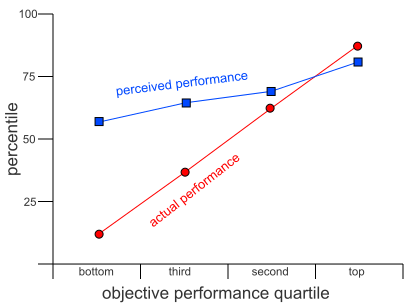
\includegraphics[width=0.95\linewidth]{images/Libro-img001.png}
  \begin{minipage}{\linewidth}
    \caption{By Phlsph7 - Own work, CC BY-SA 4.0, \protect\url{https://commons.wikimedia.org/w/index.php?curid=124703870}}
  \end{minipage}
\end{wrapfigure}

L'effetto Dunning-Kruger studiato dagli psicologi David Dunning e Justin
Kruger\endnote{\protect\url{https://it.wikipedia.org/wiki/Effetto\_Dunning-Kruger}} è una distorsione cognitiva, dove tendiamo a
sopravvalutare le nostre conoscenze. Come vediamo dal grafico a lato, quando ci cimentiamo in una nuova materia la
percezione delle nostre conoscenze (linea blu) è molto più alta delle nostre effettive competenze (linea rossa). Questo
perché avendo una conoscenza superficiale ci porta a pensare che i fondamentali siano invece una parte importante delle
competenze totali. Sappiamo quanto sappiamo ma non avendo una quadro completo non sappiamo quanro ancora
c'è da sapere per autovalutare la percentuale del totale della nostra comprensione.

Questo fenomeno è stato studiato nel 1999, ma da millenni l'uomo ne è a conoscenza:

Charles Darwin "L'ignoranza genera fiducia più spesso della conoscenza"

Bertrand Russell "Il problema dell'umanità è che gli stupidi sono strasicuri,
mentre gli intelligenti sono pieni di dubbi"

William Shakespeare "Il saggio sa di essere stupido, è lo stupido invece che crede di essere
saggio"

Socrate (Platone, Apologia di Socrate) "So di non sapere"


\bigskip

Più ci si addentra nello studio e nella conoscenza, più ci si rende conto delle infinite ramificazioni del sapere. La
conoscenza diviene pertanto un processo in divenire e mai del tutto esaurito. 


\bigskip

Ma come mai l'evoluzione ci ha dato questo effetto? 

Il nostro cervello per poter fare qualcosa per la prima volta lo simula preventivamente nella mente tramite
l'immaginazione. Vi sarà capitato anche a voi di vedere, un equilibrista, un tuffatore, un
musicista, un influencer e dire, non sembra difficile! Questo perché nella vostra simulazione mentale siete davvero
riusciti a farlo! Questo è molto utile, perché ci motiva. Se il nostro pensiero fosse orientato a tutti gli ostacoli
che dovremo superare nel nostro cammino, le cose che dobbiamo ottenere, imparare a fare, molleremmo subito! Ma è anche
un'arma a doppio taglio siccome ci può dare l'illusione di aver acquisito una
certa competenza.


\bigskip

Il contrario di questo effetto è la sindrome dell'impostore, che porta
l'individuo a credere di non meritare i propri traguardi perché crede invece essere dovuti dal
caso, dalla fortuna o dalla sopravvalutazione degli altri. Paradossalmente però, se fossi un impostore, non avresti la
sindrome dell'impostore in quanto non metteresti in dubbio le tue capacità. Non stai cercando di
truffare nessuno, ma provando solo a fare un buon lavoro. Il fatto di interrogarsi sulle proprie capacità è positivo,
ci porta a migliorare e non finire vittima dell'effetto Dunning-Kruger.


\bigskip

\subsection{Fattore culturale}
Nell'Africa sub-Sahariana, in lingua bantu esiste la parola ubuntu. Appellandosi a questa parola si è soliti dire Umuntu
ngumuntu ngabantu, {\textquotedbl}io sono ciò che sono in virtù di ciò che tutti siamo{\textquotedbl}. L'ubuntu esorta
a sostenersi e aiutarsi reciprocamente, a prendere coscienza non solo dei propri diritti, ma anche dei propri doveri,
poiché è una spinta ideale verso l'umanità intera, un desiderio di
pace\endnote{\protect\url{https://it.wikipedia.org/wiki/Ubuntu\_(filosofia)} }. Anche questo comportamento deriva dalla nostra
evoluzione. L'essere umano non ha artigli, zanne, forza e velocità sufficienti per vivere da solo
come le tigri ed essere autosufficienti. Quindi gli individui che sapevano collaborare e amalgamarsi meglio alle regole
del gruppo venivano premiati dalle risorse condivise, mentre al contrario, chi non aderiva alle norme sociali veniva
ostracizzato e allontanato dal gruppo, scelta che probabilmente avrebbe condannato alla morte
dell'individuo. 

Nel 1967 fu condotto un esperimento molto interessante per spiegare come funziona il fattore culturale nella società. Il
dottor Stephenson predispose una gabbia con una banana fissata al soffitto e, al di sotto una scala per poterla
raggiungere dalle cinque scimmie che sono state introdotte. Come possiamo immaginarci, dopo poco tempo una di queste
scimmie ha provato a raggiungere la banana, ma un getto d'acqua gelida ha travolto lei e tutte le
altre. Quando anche un'altra scimmia ha provato a raggiungere la banana, tutto il gruppo è stato
bagnato con dei getti d'acqua e, questa situazione si è ripetuta per ogni primate che tentava
l'impresa, fino a quando hanno imparato la lezione e non hanno abbandonato la missione. Arrivati a
questa situazione di stallo, il ricercatore ha rimosso una scimmia dal gruppo e ne ha introdotta una nuova, ignara di
cosa le sarebbe successo, se avesse provato a raggiungere la banana. Infatti, appena entrata, come prima cosa ha
provato a salire sulla scala per arrivare al frutto, ma è stata fermata con forza da tutto il resto del gruppo, che non
voleva passare il resto della giornata infreddolito. La scimmia che ha fatto ingresso nella gabbia per ultima ha
provato diverse volte a raggiungere la banana ma sempre con lo stesso epilogo, fino a quando anche
quest'ultima non ha rinunciato. Il ricercatore ha così sostituito un'altra
scimmia appartenente al primo gruppo, quello che ha realmente provato i getti d'acqua gelida con
una nuova, all'oscuro di questa punizione. Come successo al suo predecessore, la scimmia è stata
fermata con ogni mezzo dalle altre, anche da quell'ultima che non era mai stata bagnata.
Periodicamente i ricercatori ripetevano questa procedura, sostituendo una scimmia del primo gruppo con una nuova,
ripetendosi lo stesso comportamento per evitare che si raggiungesse la banana. Alla fine si arrivò a liberare tutte le
scimmie del primo gruppo e ad avere nella gabbia solo scimmie che non erano mai state bagnate
dall'acqua, ma che avrebbero comunque lottato per impedire che qualcuno raggiungesse la banana.

Anche per gli esseri umani e per cose ben più serie di una banana funziona esattamente così. Persino le guerre vengono
tramandate e, la gente si ammazza senza sapere nemmeno il perché. In Giamaica nel periodo di lotta per
l'indipendenza dall'Inghilterra si sono formati due partiti in lotta violenta
e armata fra loro: il People's National Party (PNP) e il Jamaica Labour Party (JLP). Nonostante la Giamaica oggi sia
indipendente, la capitale, Kingston, è una delle città più violente al mondo per tasso di omicidi.
Tutt'ora ci sono delle zone dove non ci puoi andare se sei nato in un territorio nemico, è così e
basta, non si sa più il perché, è stato solo tramandato.


\bigskip

Questo è un ulteriore tassello per comprendere quanto sia importante la consapevolezza. Se facciamo qualcosa e ignoriamo
il momento in cui abbiamo deciso di fare questa scelta e tutto il processo cognitivo che l'ha
preceduta, molto probabilmente è un comportamento appreso dagli altri e non dalla nostro pensiero. Questo succede a
tutti, ma è importante ripensare a ciò che facciamo o se possibile accorgerci mentre ci capita e interrogarci,
chiedendoci se questa azione è in linea con i nostri valori, altrimenti saranno gli altri ad aver scelto per noi e
saremmo inautentici.


\bigskip

Io, per esempio ho avuto la fortuna di creare uno stile di vita che fosse tutto mio, o forse sono semplicemente un
bastian contrario e quindi sono sempre gli altri ad aver deciso per me. Mi è capitato di conoscere persone che, la sera
stessa che ci siamo conosciuti e, appena saputo che non bevevo alcol, non hanno avuto nessun imbarazzo nel darmi dello
“sfigato” seppure non fossimo amici e nemmeno conoscenti. Non sono immune alle critiche come chiunque, ma ho avuto la
fortuna, perché non ho mai lavorato su questo mio aspetto, che alcune cose non mi feriscono e sono così riuscito a dare
una direzione alla mia vita che credo aver abbastanza protetto dalle influenze esterne. Però per qualcuno è più
difficile e questo è un peccato che qualcuno possa sentirsi inadeguato, diverso, a disagio nonostante faccia scelte
positiva e/o innocue, in quanto, in questo caso, non crea problemi agli altri siccome possono continuare a bere e,
seguire lo stile di vita che preferiscono. Anche questo è un esempio di come il Sistema si mantiene compatto, senza un
apparente motivo, o vantaggio per qualcuno, senza qualcuno che tiri i fili delle persone, ma sono esse stesse a farsi
promotrici del mantenimento dello status quo. 

Per questo, per dare alla vita la direzione che vogliamo ed essere autentici, dobbiamo imparare ad essere talvolta
deludenti per gli altri, ma ci ritorneremo più avanti.


\bigskip
\begin{mdframed}[linewidth=1pt]
Stigma del fallimento

Noi europei, in particolare gli italiani, viviamo lo stigma del fallimento con vergogna. Dobbiamo essere sempre
perfetti, sempre sul pezzo, informati, produttivi, risolutivi, ma questo è impossibile in un mondo complesso dove
l'asticella continua ad alzarsi. Dobbiamo accettare l'incertezza, come unica
costante della vita. Accettare che non c'è nulla di male se non sappiamo fare qualcosa, se non
conosciamo qualcosa, se abbiamo bisogno di aiuto o se falliamo. La storia è piena di esempi:

Thomas Edison raccontò che fece diecimila tentativi prima di riuscire ad accendere la prima lampadina. Dicendo: Non ho
fallito. Ho solo trovato diecimila modi che non avrebbero funzionato. Come dargli torto col senno di poi, il risultato
del suo lavoro lo utilizziamo tutti i giorni. Henry Ford affrontò due crac, poi fondò la Ford Motor Company. Un
progetto di Steve Jobs fece flop e lui fu licenziato dalla sua stessa Apple. Bill Gates creò una società per
ottimizzare i flussi di traffico attraverso l'analisi di dati, chiamata Traf-O-Data. Persino
Donald Trump ha una lunga lista di crac e
fallimenti\endnote{\protect\url{http://lettura.corriere.it/debates/il-fallimento-e-un-diritto/} }.


\bigskip

Non avrai mai fallito finché continuerai a provare (Anonimo).


\bigskip

Oltre oceano il fallimento viene visto come un processo naturale, quasi obbligatorio per raggiungere un obiettivo. In
particolare, nella Silicon Valley, si cita frequentemente, come un mantra, “fallire velocemente, fallire spesso”. Ogni
fallimento può essere analizzato e, una volta individuati i problemi, farne tesoro per aggiustare il tiro e, fare
meglio la volta successiva. Insomma, sbagliando si impara! L'abbiamo sentito tante volte ma ancora
non l'abbiamo compreso appieno.


\bigskip

La distorta ricetta della perfezione ha portato l'Europa, all'idea del
fallimento come una vergogna da confessare in pubblico. La pressione sociale, le sue aspettative, il senso di colpa,
l'ansia, diventano talmente elevate da risultare insostenibili, portando a disistima e perdita di
identità. Il fallimento viene così vissuto come marchio indelebile agli occhi della società e non come un viaggio alla
scoperta di sé, dei propri limiti e dei propri talenti.

Non è un caso che quando sperimentiamo cose nuove, cerchiamo di farlo da soli. Se sbagliamo e, siamo da soli, non è un
problema, perché nessuno si è accorto, è come se non fosse mai successo. Lo stesso identico errore davanti ad altri
invece viene vissuto con vergogna e afflizione. Tutti nutriamo timori di fallire, il che favorisce il proliferare del
dogmatismo, delle echo-chamber e della ricerca di contesti e gruppi che vanno dai fanatici, agli estremisti, ai
complottisti, in cui le nostre idee non possono mai essere considerate fallimentari. Da piccoli quando inciampavamo,
non stavamo a rimuginare su cosa pensavano gli altri, su come fosse potuto accadere, su cosa avremmo potuto fare,
semplicemente ci rialzavamo e continuavamo, senza giudicarci. In questo modo il male della caduta scorreva via
naturalmente e non veniva trattenuto coi nostri pensieri. Questo è un modo funzionale di vivere il fallimento.

Non possiamo essere una risposta per gli altri.


\bigskip

Il successo è, in realtà, la somma di tutti i nostri fallimenti

Francesca Corrado


\bigskip

Forse l'intuizione di Freud che identifica il problema nella repressione dei desideri come problema psicologico non é
più attuale. Perché siamo passati da una società della disciplina a una società dell'efficienza dove l'angoscia non è
più nel conflitto tra desiderio e repressione, quanto nell'ansia di essere all'altezza delle richieste lavorative,
sociali ecc...


\bigskip

“Io non perdo mai: o vinco o imparo.” - Nelson Mandela 


\bigskip

Anzi, se non fallisci mai è perché probabilmente ti sei posto obiettivi troppo poco ambiziosi. dovremmo stabilire una
parte di obiettivi raggiungibili e, una parte, attorno al 30/40\% di obiettivi straordinari, più difficili da
raggiungere e che potrebbero fallire. Quindi se fallisci non è motivo di vergogna, magari era un obiettivo giustamente
ambizioso, forse troppo per quel momento, ma non in assoluto. 

Chi resta fermo non fa errori, per cui quando sbagli, gioisci perché stai progredendo.
\end{mdframed}

\bigskip

\subsection[De{}-responsabilizzazione]{De-responsabilizzazione}
Verso la metà del 900, lo psicologo J. B. Rotter parlò di “Locus of control” (“luogo di controllo”) ovvero, la
percezione di quanto la propria vita sia influenzata dalle proprie azioni o dalla casualità e, di conseguenza, a quali
di questi due fattori si attribuiscono successi e insuccessi. Negli ultimi la tendenza sembra essersi spostata
sull'attribuire a fattori esterni gli insuccessi e a fattori interni, dipendenti dal proprio
agire, i successi. Il motivo è semplice, è “comodo” dire che se qualcosa va bene è merito mio e se va male è colpa
degli altri, ma questa è un arma a doppio taglio. Apparentemente ci stiamo proteggendo la nostra autostima in questo
modo, in realtà ci stiamo privando di avere la percezione di poter agire e intervenire sul mondo. Ovviamente non
possiamo \ pensare che tutto sia sotto il nostro controllo, se lo credessimo cadremmo in altre problematiche, come
detto in precedenza dobremmo pian piano imparare ad accettare l'incertezza. Ma agire come se tutto
fosse influenzabile da noi, ci dona auto efficacia. Se qualcuno ci tratta male, anche se lui rimane il maleducato, ma
ci chiediamo: come posso pormi prossima volta per evitare questa reazione? O ancora, posso aver agevolato in qualche
modo questa reazione? Questo atteggiamento ci dona una possibilità di cambiamento. Se invece pensiamo che lui ha
sbagliato e basta, cosa che potrebbe anche essere vera, ci poniamo in una condizione dove noi siamo in balia degli
eventi, completamente inefficaci di gestire le situazioni che ci accadono. Lo psicologo e filosofo William James dopo
numerosi problemi ha pensato di togliersi la vita, ma prima, ha fatto una scommessa con se stesso. Lui ha iniziato a
vedere tutto ciò che gli capitava nella sua vita, come se lui fosse il solo responsabile e se dopo un anno le cose non
fossero migliorate, allora si sarebbe suicidato. Fortunatamente questa storia ha un lieto fine e James non si suicidò.

Una cosa su cui sono piuttosto sensibile è proprio questo tipo di narrazione, mi sembra che si cerchi prevalentemente un
colpevole più che una soluzione. Che si tratti del partner, dell'insegnante, della dirimpettaia,
del governo o delle scie chimiche. Di esempi ce ne sono tanti, un collega o un superiore che incolpa la mancata
consegna di un lavoro mal schedulato da lui. Una mamma che incolpa gli insegnanti per i pessimi voti del figlio,
l'insegnante per il disimpegno degli studenti, gli studenti dicendo che la loro scuola fa schifo,
non argomentando con un generico: “non c'è organizzazione”, manca il lavoro e così via
all'infinito.

Quante volte capita di dire: “è colpa del governo”, nel paese dove c'è la più alta evasione
fiscale, dove si timbra il cartellino del collega che è rimasto a casa, farsi dare la malattia
dall'amico medico, i finti invalidi, parcheggiare in doppia fila, nel posto degli invalidi, fare
contratti da precari o non farli affatto, vendere con un sovrapprezzo mascherine, guanti, gel igienizzanti in periodo
di pandemia (questa l'ho scritta a marzo 2020), piccoli furti ecc… quanti italiani sono
impeccabili? Pochi e, quanti si lamentano della società? Tanti. È chiaro che se non si paga le tasse il governo ha meno
soldi da spendere per fare qualcosa per la collettività. Questa è de-responsabilità!


\bigskip

\subsection{Suggestioni}
Effetto Priming\endnote{\protect\url{https://it.wikipedia.org/wiki/Priming\_(psicologia)} }: Questo effetto dice che
l'esposizione a uno stimolo influenza la tua risposta. \newline
Il priming ci influenza su tutto, anche un fresco venticello in una giornata torrida ci fa essere più positivi, o al
contrario, se ci rechiamo in un ristorante e abbiamo litigato con un automobilista apprezzeremo molto meno il cibo. Un
test ha dimostrato che se scriviamo parole come: correre, veloce, rapido e poi, a fine test andiamo a consegnare il
nostro foglio, percorreremo il corridoio molto più velocemente di un altro che ha scritto parole come: lento, piano,
tranquillo ecc.. \ Altri esempi: Se fa caldo diventiamo più aggressivi, se piove saremo più critici, se si ha fame si è
più impulsivi. Ricordi cosa abbiamo detto del libero arbitrio?

Quanto detto è contrario alla filosofia: fake it until you make it, ovvero, fingi fino a quando non lo ottieni, figlia
di alcuni movimenti motivazionali, che grazie a frasi automotivazionali promettono di farti raggiungere certi risultati
personali e farti diventare una persona diversa. In realtà, queste tecniche sono molto potenti ed efficaci, spesso si
utilizzano quando un atleta deve affrontare una gara. Queste tecniche però possono essere pericolose, perché, se
immaginiamo tante volte noi che riusciamo a superare una difficoltà, quando si presenterà davvero, abbasseremo la
guardia e l'impegno perché convinti di saper gestire quella determinata situazione. Essere in uno
stato mentale negativo e credere di non farcela ti porterà a non farcela, ma al contrario, se noi siamo sicuri di
farcela questo non sarà sufficiente a garantirci il successo. Quindi va bene prefigurarsi un nostro stato mentale o le
varie ipotesi, ma tenendo sempre presente che le nostre aspettative potrebbero non realizzarsi. Questo effetto però
agisce solo fino ad un certo punto, non può cambiare la nostra personalità o il nostro umore sul lungo periodo. Se sei
un atleta e ti influenzi affinché tu ti senta più forte e concentrato, la tua performance sarà migliore, ma è solo la
cigliegina sulla torta, alla base deve esserci un duro allenamento. Non basta ripetersi di essere milionari o felici
per diventarlo. Allo stesso modo vale anche al contrario, se mi dico che sono un imbranato, non è che lo diventerò.
Basta solo la consapevolezza, senza analisi o costruzioni logiche. È per questo che le suggestioni, le frasi
motivazionali non funzionano, perché sai che ti stai suggestionando. Le suggestioni funzionano solo se sono nascoste e
non ne siamo consapevoli, come la pubblicità per esempio. Anche Facebook nel 2012 condusse un esperimento con oltre 680
mila utenti, esponendoli a contenuti per la maggior parte positivi, per un gruppo e negativi per
l'altro. Il risultato fu che gli utenti pubblicavano post negativi se leggevano prevalentemente
post negativi e viceversa.

Un altro esperimento condotto dallo psicologo evoluzionista Douglas Kenrick chiese a un gruppo di uomini in quale misura
fossero soddisfatti della propria partner. Prima di compilare il questionario a metà dei soggetti vennero fatti
consultare libri di arte astratta e all'altra metà, riviste di Playboy. Come avrete già intuito il
secondo gruppo riportò gradi di soddisfazione inferiori rispetto al primo gruppo e, questo può essere un problema se
pensiamo a quanto l'attuale società ci bombardi con le sue pubblicità.

Un altro effetto interessante che ci condiziona inconsapevolmente è l'effetto placebo e anche il
suo opposto meno noto effetto nocebo. L'effetto nocebo è un condizionamento in negativo, se
diciamo a una persona che questo macchinario potrebbe provocarti del dolore, probabilmente lo farà, anche se si tratta
di una lampada che fa un leggero calore\endnote{\protect\url{https://youtu.be/OUdXMoY6fLY} }.


\bigskip

\subsection{Altre distorsioni comuni}
Errori di ragionamento chiamate fallacie induttive, ovvero, pensare che se è successo una volta allora succederà sempre.
Se una cosa è vera una volta allora lo sarà sempre. Vediamo alcuni esempi:

\begin{itemize}
\item Generalizzazione indebita: Un uomo ha rubato una mela. Quindi tutti gli uomini sono ladri.
\item Generalizzazione statistica: Su un campione di 500 adolescenti italiani, dove l'80\% naviga in internet per più di
tre ore al giorno. Significa che l'80\% degli adolescenti italiani naviga in internet per più di tre ore al giorno.
L'errore qua è aver utilizzando un campione insufficiente, 500 persone infatti, risulta un numero
troppo basso, non significativo.
\item Fallacia del giocatore: Se gioco alla alla roulette ed è uscito il rosso per cinque volte, molto probabilmente ora
uscirà il nero. Statisticamente invece ogni volta, rosso e nero hanno la stessa probabilità di uscire, infatti non sono
rare sequenze di venti colori tutti uguali in questo gioco. Su questa fallacia si basa il metodo Croce, che promette
guadagni certi in questo gioco.
\item Falsa causa: Ho rotto uno specchio e ora va tutto storto. La scaramanzia, ma non solo, rientra in questa
tipologia, quando si cerca di spiegare qualcosa con una causa la quale non è strettamente legata con
l'effetto
\item Fallacia dell'evidenza soppressa: Nelle prossime pagine vedremo alcuni esempi. In sostanza si tratta di omettere
delle informazioni importanti e che quindi daranno una visione della questione anche diametralmente opposta.
\end{itemize}

\bigskip

Si parla di fallacie di presupposizione quando le premesse sono anche le conclusioni della nostra tesi, per indurre
l'interlocutore alla stessa soluzione.

\begin{itemize}
\item Fallacia patetica: Credere che tutto si comporti con una logica umana. Ad esempio agli umani piace essere liberi,
quindi anche l'aria e, per questo esiste la pressione in fisica. O la paura che i robot e
l'intelligenza artificiale un giorno si ribelleranno e conquisteranno il mondo. La conquista del
mondo o la prevaricazione su altre specie non la ritroviamo in natura, è un ambizione del tutto umana, è un errore
quindi pensare che un robot umanoide abbia i medesimi desideri.
\item Circolarità semplice: Tra le premesse di un'argomentazione figura la tesi che si vuole sostenere. Per esempio: Dio
ha creato il mondo, dunque Dio esiste. Dio esiste, dunque è stato Dio a creare il mondo.
\item Domanda multipla: quando nella domanda si dà per scontato qualcosa che non è stato ancora dimostrato. Esempio: Mi
spieghi come hai fatto a copiare il compito in classe?
\item Fallacia della conclusione sbagliata: Ad esempio dimostriamo che l'inflazione sta scendendo e
ne concludiamo che l'economia sta andando bene. Le premesse però non sostengono la conclusione.
\item Falsa pista: Esempio: Il Paese è sotto la minaccia del terrorismo. Urge acquistare nuovi armamenti sempre più
potenti. Il terrorismo non si combatte necessariamente con l'acquisto di nuovi armamenti. Possono essere efficaci anche
quelli già in dotazione, si può aprire una trattativa, un dialogo ecc…
\item Argomento fantoccio: confutare una tesi apparentemente simile a quella che si vuole negare o confermare così, per
conseguenza logica, cade o viene confermata anche la tesi principale. Esempio: Darwin ha commesso questi errori, quindi
tutta la teoria dell'evoluzione è falsa.
\end{itemize}

\bigskip

Fallacie formali e informali

\begin{itemize}
\item Argomentazione a catena: Si giunge a una conclusione erronea tramite un processo di reazione a catena, come ad
esempio, chi prova le droghe leggere come la cannabis, arriverà a provare anche la cocaina, perché cercherà sempre
qualcosa di più forte.
\item Tu quoque: X sostiene che si dovrebbero pagare le tasse, ma siccome X è un evasore fiscale, le tasse non vanno
pagate.
\item Accusa d'interesse: Se c'è un conflitto d'interesse allora
l'oggetto in discussione è necessariamente falso.
\item Colpa per associazione: X sostiene una testi, ma X è anche amico di spacciatori. Quindi X non è una persona
rispettabile e la sua tesi di conseguenza.
\item Appello all'autorità: Prendere per vera o falsa una tesi perché “l'ha detto X”. Il classico
ipse dixit o “l'ha detto la televisione”.
\item Appello alla modestia: Al contrario dell'appello all'autorità, si è portati a credere a una teoria minore, di
nicchia e, non ancora riconosciuta.
\item Ad judicium: Se lo dicono tutti allora sarà vero. Da qua nascono i miti! Ne cito alcuni di quelli che abbiamo
sempre creduto veri e invece sono falsi: scrocchiare le dita fa venire l'artrite, stare troppo vicino alla TV rovina
gli occhi, il freddo fa ammalare, se cade qualcosa per terra per meno di cinque secondi si può mangiare, il cioccolato
fa venire i brufoli, lo zucchero di canna è più salutare di quello bianco. Le affermazioni appena citate sono tutte
false\endnote{\protect\url{https://www.focus.it/scienza/salute/bugie-salute}.}
\item Argumentum ad ignorantiam: Si giustifica la propria tesi con la mancanza di prove del suo contrario.
\item Fallacia della brutta china: Fa appello alle conseguenze negative della tesi da rigettare.
\end{itemize}

\bigskip

Altre distorsioni:

\begin{itemize}
\item Bias di conferma: credere a informazioni che confermano ciò che già sappiamo. Questo è uno degli effetti più
frequenti e citati che porta ad altri effetti come il \ Dunning Kruger, echo chamber e filter bubble. Questo effetto è
molto insidioso perché spesso noi agiamo per esempi negativi piuttosto che per esempi positivi. Se qualcuno ci sta
antipatico, inizieremo a leggere, informarci, allenarci di più, solo per potergli andare contro. Forse non sono le
motivazioni più nobili, ma funzioniamo così e può portare a risultati positivi, se riusciamo a non cadere in questo
bias.
\item Effetto invorniciamento: presentare una teoria mostrando solo aspetti negativi o positivi influenza il giudizio.
Anche il contesto é importante, uno sconto a tempo ci farà essere più frettolosi nell'acquisto 
\item Bias del costo sommerso: Portare avanti un lavoro, un progetto, o una relazione solo perché interrompendola si
perderebbero tutti gli investimenti di tempo soldi e energie passate
\item Euristica dell'affetto: Sento di fare così quindi è giusto. Valutazione di pancia senza valutazione oggettiva 
\item Euristica della disponibilità: Ad esempio quando il telegiornale parla sempre di una cosa, che magari é un evento
raro ma ci inizia a sembrare invece molto frequente 
\item Astrazione selettiva: si presta attenzione ad un solo aspetto o a un solo dettaglio della situazione. Gli aspetti
positivi sono spesso ignorati a vantaggio di quelli negativi o viceversa.
\item Pensiero dicotomico: gli eventi sono valutati in forma estrema, del tipo buono / cattivo, nero / bianco, on / off,
etc.
\item Inferenza arbitraria: vengono tratte conclusioni da situazioni non supportate dai fatti, anche quando
l'evidenza è in contrasto con la conclusione.
\item Supergeneralizzazione: si giunge a una conclusione generale partendo da un evento particolare.
\item Ingigantire e minimizzare: si assume la tendenza a esagerare gli aspetti negativi di una situazione, riducendo al
minimo il positivo.
\item Personalizzazione: vengono attribuite caratteristiche personali a una situazione.
\item Visione catastrofica: si anticipano gli eventi pensando che il peggio accadrà sicuramente.
\item Doverizzazione: ci si auto-impone regole rigide e severe su come le cose dovrebbero andare.
\item Variabili globali: vengono utilizzate etichette generali sugli eventi che non considerano le diverse sfumature.
\item Bias di ancoraggio: propensione a prendere decisioni basandosi sulle prime informazioni trovate, utilizzate come
riferimento per i ragionamenti successivi. Per esempio, il primo prezzo offerto per un'automobile di seconda mano
imposta lo standard per il resto della negoziazione. Un prezzo inferiore sembrerà ragionevole anche se superiore al
vero valore dell'automobile.
\item Apofenia: nota anche come patternicity, o agenticity, è la tendenza umana a trovare spiegazioni, soluzioni,
schermi ricorrenti tra dati casuali e senza una vera spiegazione statistica.
\item Hindsight bias: o bias del senno di poi è la tendenza delle persone a credere, erroneamente, di aver saputo
prevedere un evento correttamente, una volta che l'evento è ormai noto. 
\item Outcome bias: o bias del risultato è la tendenza a rileggere il passato con gli occhi e
l'esperienza di oggi modificando la storia attorno a quell'evento.
\item Bias dei dettagli seduttivi: Valutare un argomento come convincente se supportate da informazioni che seppur veri
ma che a pensarci bene non hanno nessuna correlazione con la
questione\endnote{\protect\url{https://www.stateofmind.it/2018/07/distorsioni-cognitive/} }
\endnote{\protect\url{https://it.wikipedia.org/wiki/Bias\_cognitivo} }. 
\end{itemize}

\bigskip

Queste sono solo alcune delle fallacie studiate. Abbiamo anche quelle che fanno appello alle emozioni, che portano a
cambiare opinione per paura o compassione, usate molto in televisione\endnote{\protect\url{https://it.wikipedia.org/wiki/Fallacia}.}


\bigskip

\subsection{Libero Arbitrio}
Prendiamo decisioni attraverso schemi mentali o automatismi fallaci, bias cognitivi, di cui non ci rendiamo conto. I
bias cognitivi che abbiamo visto precedentemente sono comuni a tutti noi, con percentuali più o meno diverse. In più,
ognuno di noi sviluppa degli schemi mentali suoi, che sono unici, ma di cui non sempre ne è a conoscenza, ma da cui
dipende tutta la propria vita e le proprie decisioni. Proprio ora, mentre stai leggendo, sei consapevole della tua
posizione? Come sono posizionati i tuoi arti? Qualcuno di voi avrà le gambe accavallate, incrociate, o con una mano che
sorregge la testa ecc… Ora che l'hai letto, sei consapevole della posizione che ha assunto il tuo
corpo, ma fino a un attimo fa no. Eppure è stato il tuo cervello a metterti in quella posizione e, continuava a mandare
impulsi affinché tu mantenessi quella posa. Hai scelto di metterti in quella posa? O l'ha scelto
il tuo cervello? E come mai ha scelto proprio quella e non un'altra? A volte capita che guidando
l'auto per andare al supermercato, siamo sovrappensiero e ci ritroviamo a casa. Oltre a gestire
tutti i nostri sistemi, che ci consentono di sopravvivere, come far battere il cuore, respirare ecc… il nostro cervello
è sempre in ascolto dei nostri cinque sensi. Se ci arriva qualcosa in faccia all'improvviso,
chiudiamo gli occhi, giriamo la testa e ci proteggiamo con le mani, senza nemmeno pensarci. Se in una stanza rumorosa
stiamo leggendo, riusciamo a isolarci da tutte le parole e, riusciamo a non seguire i discorsi degli altri, ma se
qualcuno ci chiama, noi ci accorgiamo. Questo vuol dire che in realtà il nostro cervello ha analizzato tutti i suoni,
li ha convertiti in parole, li ha analizzati e deciso autonomamente che tutte le parole non dovevano essere mostrate
alla consapevolezza, alla nostra attenzione, tranne una, che invece poteva interessargli. Questi automatismi, questi
nostri schemi mentali, riguardano solo queste azioni automatiche? In realtà no, come vedremo nel capitolo sui
dibattiti, le nostre decisioni sono prese perlopiù da un fattore emotivo. Decidiamo che una cosa sia giusta o sbagliata
in base a quello che ci piace o no e, in un secondo momento, giustifichiamo la nostra scelta. Convinciamo noi stessi.
Anche quando cerchiamo di prendere una decisione con il ragionamento, mettendoci in discussione, con il massimo
dell'onestà intellettuale, il nostro dialogo interiore, che potrebbe affrontare la discussione in
infiniti modi e, punti di vista, dovrà per forza scegliere un percorso e, quest'ultimo verrà
dettato ancora una volta dai nostri schemi mentali. 

Esattamente come successo nell'esempio sulla tua postura in questo momento, il cervello, prima
prende una decisione e, poi te la comunica. Quando diventi consapevole di questa decisione, credi di averla presa tu,
in realtà l'aveva già presa qualche millisecondo prima il tuo cervello. Qui sta
l'illusione del libero arbitrio. Il nostro cervello ha sviluppato quindi questa strategia per
essere più efficiente, prendere decisioni immediate, come i riflessi, senza sottoporle alla coscienza, che è lenta
nell'elaborazione. Il cervello, per essere veloce, non mette in discussione ogni singola
questione, anzi, non lo fa quasi mai. Il cervello approssima, etichettando, dando un nome a un determinato fenomeno e,
attuando per tutti la stessa soluzione che ha visto funzionare in passato per un evento che reputa dello stesso tipo.
Questa strategia è efficiente in termini di velocità decisionale ma non nell'accuratezza. Questa
strategia si chiama pregiudizio, ovvero, giudicato prima, prima di un'attenta, ma lenta analisi.
Il nostro cervello ha bisogno di ordine, necessita di dare un senso a tutto, anche a quello che non conosce, per questo
si può finire nella superstizione, al credere alla religione, l'oroscopo, complotti ecc… La vita
moderna ci sottopone continuamente a una moltitudine di informazioni, di sollecitazioni e il nostro cervello non può
stare dietro a tutto. Così, gli stessi schemi mentali o automatismi, necessari e che funzionano bene per la grandissima
maggioranza di casi, vengono riproposti anche per tutto il resto. Anche decisioni etiche e morali. Ma come si formano
gli schemi mentali? Il nostro cervello e formato da neuroni che sono collegati tra loro da sinapsi. Se dobbiamo
raggiungere un luogo che non conosciamo, per esempio un nuovo posto di lavoro, la prima volta chiederemo informazioni,
guarderemo i cartelli, alla fine riusciremo ad arrivare fino alla nostra destinazione, magari un po' a tentativi anche
e, facendo strade sbagliate. Questa nostra esperienza avrà creato delle nuove connessioni neuronali, delle sinapsi. Ora
abbiamo diversi nuovi collegamenti, anche se deboli. Il giorno dopo ci troveremo a raggiungere nuovamente il posto di
lavoro, abbiamo capito la zona e fino a li ci arriviamo senza problemi, magari sbagliamo ancora un paio di svolte, ma è
comunque andata meglio del giorno prima. Con questa nuova esperienza, inizieremo a rafforzare alcune connessioni
neuronali e abbandonarne altre. I primi giorni impareremo a raggiungere il luogo di lavoro, in più, sperimenteremo
nuove strade, per metterci meno tempo, evitare il traffico ecc… Una volta che troviamo la strada secondo noi migliore,
tutti i giorni percorreremo sempre la stessa strada e quelle connessioni neuronali, che ci permettono di raggiungere il
posto di lavoro, facendo quel preciso percorso, diventano sempre più forti, creando uno scherma mentale forte. Quando
si hanno connessioni forti si ha meno elasticità mentale. Per questo può essere utile fare alcuni esercizi come,
cambiare sempre strada per tornare a casa o sedersi a tavola in posti diversi da quelli usuali.

Negli anni alcuni scienziati hanno cercato delle prove circa l'illusione del libero arbitrio.
Benjamin Libet chiese a dei volontari di premere un pulsante che si trovava davanti a loro e, potevano farlo in
qualsiasi momento, quando lo preferivano. I partecipanti all'esperimento sono stati monitorati con
un elettroencefalogramma. Il risultato fu che l'attivazione sensoriale avveniva circa mezzo
secondo prima che il partecipante all'esperimento prendesse consapevolezza di premere il pulsante.
Forse può sembrare un tempo irrisorio, ma per il sistema nervoso, dove le informazioni viaggiano a centinaia di metri
al secondo è un tempo lunghissimo. Nel 2008 è stato riproposto un esperimento simile\endnote{C. S. Soon,
"Unconscious determinants of free decisions in the human brain", Nature
Neuroscience}, ma questa volta utilizzando una risonanza magnetica che può offrire informazioni più precise. In più i
partecipanti questa volta potevano scegliere tra due diversi pulsanti. I ricercatori potevano sapere con un anticipo,
anche di secondi, se il partecipante avrebbe premuto il pulsante destro o sinistro.


\bigskip

A seguito di questi esperimenti lo psicologo americano Wegner, intuì che è il cervello a decidere, non la nostra
volontà. Il cervello decide secondo lo schema mentale che si è costruito negli anni, in base alle cose casuali che
captava nell'ambiente attorno a lui e, in parte anche grazie alla sua genetica. Una volta che il
cervello ha preso la sua decisione genera nell'individuo la sensazione della volontà.
L'uomo non decide le proprie azioni, ma semplicemente gli accadono.

Se hai avuto la fortuna, la casualità, di vivere in un ambiente che ti ha fornito condizionamenti positivi, che ha
permesso lo sviluppo di certe connessioni neuronali, sarai più avvantaggiato rispetto a una persona che, sempre
casualmente, è cresciuta in un ambiente che gli ha fornito uno schema mentale il quale non lo porta a reagire o che lo
fa soffrire. A questo va aggiunto una componente genetica anch'essa pseudo casuale, su cui non
abbiamo potuto avere controllo. E come vedremo successivamente non accettare questi schemi, ignorarli, fare finta che
non esistano, può portare a problemi.

Anche questo esperimento va visto nella giusta prospettiva, nella sua “via di Mezzo”. Premere un pulsante è un
operazione semplice, molto soggetta ad automatismi e, grazie ai neuroni specchio il cervello attiva le stesse aree
celebrali sia nel fare una certa azione che al semplice pensiero della stessa. Potete trovare questo esperimento e
molti altri all'interno dell serie Mind
Field\endnote{\protect\url{https://www.youtube.com/watch?v=lmI7NnMqwLQ\&list=PLZRRxQcaEjA4qyEuYfAMCazlL0vQDkIj2\&index=5} }.

Un altro esperimento interessante è stato svolto in America nel periodo John Kerry e George W. Bush. Sono stati presi
due gruppi di cittadini, democratici e repubblicani, a cui sono stati mostrati dei video, dove i due politici cadevano
in evidenti contraddizioni. I democratici percepivano le contraddizioni del presidente repubblicano. Ma non percepivano
le contraddizioni del politico democratico. E viceversa succedeva per i repubblicani. Non solo perché le persone
sottoposte all'esperimento esprimevano verbalmente questa sensazione, ma anche a livello celebrale
che è stato monitorato grazie all'uso dell'elettroencefalogramma.

Altro esperimento interessante, svolto in un'università americana: Sono state prese delle
matricole, ragazzi appena iscritti, che ancora non conoscevano i professori che avrebbero avuto durante
l'anno. I ricercatori hanno mostrato ai ragazzi brevi video di trenta secondi circa, dei
professori che avrebbero avuto durante l'anno e, in base a questi, di fare una classifica dei
docenti migliori, in base a questa prima impressione. A fine anno, i ragazzi hanno avuto modo di conoscere davvero i
professori visti in quei video, ed è stato chiesto loro di rifare nuovamente la classifica dei professori più bravi.
Questa volta con cognizione di causa. Il risultato fu che la classifica è rimasta sostanzialmente invariata. Anche in
questo caso, la prima impressione, il pregiudizio inconscio ha condizionato la mente conscia e la parola. Prima arriva
la sensazione e poi la consapevolezza e la parola\endnote{\protect\url{https://www.youtube.com/watch?v=NHB-qw9XlXI} }.
Generalizzando, noi agiamo e successivamente giustifichiamo il nostro agire, come se l'avessimo
scelto noi. Questo fenomeno è stato dimostrato anche in un esperimento che coinvolgeva un bar dove principalmente si
vendevano bibite gassate. Cambiando la disposizione dei prodotti e dell'arredamento in modo da
favorire il consumo di acqua, si notò che le vendite aumentarono. Così, è stato chiesto alle persone come mai avessero
scelto di comprare l'acqua che risposero: perché ne avevamo voglia. Noi sappiamo che questo non
poteva essere vero, in quanto, prima del cambio di arredamento si è sempre preferito comprare bibite gassate. Questo ci
suggerisce che noi agiamo grazie ad una concomitanza di fattori tra cui quelli ambientali e poi, successivamente,
giustifichiamo questa nostra scelta, non facciamo il contrario. Questo effetto può essere usato anche a nostro favore,
infatti, se vogliamo cambiare una nostra abitudine possiamo intervenire sull'ambiente che ci
circonda, in modo da agevolare un certo comportamento.

Un giorno, Freud si trovava alla festa di Capodanno organizzata da Jean-Martin Charcot, uno dei suoi mentori a Parigi
durante i suoi studi sull'ipnosi. Charcot, per dimostrare la sua abilità ipnotica, ipnotizza un uomo e gli ordina di
aprire l'ombrello al centro della sala quando scocca la mezzanotte. Freud, incuriosito, segue l'uomo e gli chiede il
motivo dell'apertura dell'ombrello. L'uomo risponde che lo sta facendo perché piove, ma Freud gli fa notare che sono al
chiuso. L'uomo, incapace di rispondere adeguatamente, continua a cercare una spiegazione, dicendo che ne aveva voglia,
senza rendersi conto di essere stato ipnotizzato e di seguire degli ordini. Freud riflette su come questa situazione
possa riflettersi nella vita di tutti i giorni. Si chiede se i suoi problemi derivino dal fatto di essere stato
condizionato dalla cultura familiare e sociale, senza rendersene conto. Capisce che molte volte, quando cerchiamo di
giustificare le nostre azioni, in realtà stiamo solo razionalizzando delle difese psicologiche, piuttosto che
comprendere veramente le nostre motivazioni profonde. Questo porta Freud a interrogarsi sul ruolo dell'ipnosi nella
formazione dei comportamenti umani e nel processo decisionale.

Quindi dobbiamo arrenderci al destino? Qualsiasi nostro sforzo è inutile perché tutto è già stato scritto?
Fortunatamente no, altrimenti dovremmo aprire tutte le carceri e lasciare a piede libero gli assassini in quanto non
avrebbero colpa. Da una parte, sembra che sia davvero così. Alcuni studi dimostrano che gli psicopatici hanno alcune
aree del cervello meno sviluppate, sono nati così, non ci sono diventati. Altre persone compiono omicidi di massa a
seguito di un tumore al cervello, anch'esso, non deciso e voluto da loro. Alcuni ricercatori,
nelle carceri, dividendo i carcerati per crimine commesso, hanno notato che ogni gruppo presentava particolari geni
meno frequenti negli altri gruppi. Emblematico il caso del giudice Hannover che ha dato un fortissimo sconto della pena
per lo stupro di una ragazza. La motivazione? Lo stupratore era sardo. "Si deve tenere conto delle
particolari impronte culturali ed etniche dell'imputato. È un sardo. Il quadro del ruolo dell'uomo e della donna,
esistente nella sua patria, non può certo valere come scusante me deve essere tenuto in considerazione come
attenuante".
\endnote{\protect\url{https://www.lagazzettadelmezzogiorno.it/news/home/65714/germania-torturo-una-ragazza-sconto-di-pena-e-sardo.html}
}


\bigskip

Noi abbiamo la scelta, ma ci comportiamo con schemi seppur complessi, potenzialmente prevedibili, se potessimo leggere
nel cervello. \ Riprendendo l'esempio della strada per andare al lavoro, i nostri schemi mentali,
diventano automatici dopo un'elaborazione della mente conscia, più
l'influenza della genetica e di altri schemi mentali pregressi, più la casualità degli eventi. Tra
tutti questi punti abbiamo l'elaborazione della mente conscia su cui possiamo avere un minimo di
manovra. Un minimo perché la nostra mente conscia è comunque influenzata dalla mente inconscia, schemi mentali, bias
cognitivi, preconcetti ecc… Quindi non va visto come un destino scritto nelle stelle. È qualcosa di più locale, è la
nostra mente che ci condiziona, che ci da una “tendenza” seppur molto forte a comportarci e pensare in un certo modo.
Secondo il neurofisiologo statunitense Benjamin Libet in un esperimento sul libero arbitrio simile al precedente che
abbiamo visto\endnote{\protect\url{http://nc.oxfordjournals.org/content/2015/1/niv009} }, da quando diventiamo consapevoli di
premere un pulsante e la vera e propria azione abbiamo circa 200 millisecondi di tempo. In questo lasso di tempo
possiamo esercitare la nostra volontà e scegliere di agire
diversamente\endnote{\protect\url{https://www.focus.it/comportamento/psicologia/lorigine-dellimpulsivita} }. Come dimostrato anche
da uno studio dell'Università del New South Wales\endnote{\protect\url{https://www.nature.com/articles/s41598-019-39813-y} }
utilizzando una risonanza magnetica, si dimostra come il cervello sia “predisposto” a un tipo di scelta già prima della
formulazione conscia della decisione. I risultati di tutti i test di questo genere, seppur superino la soglia della
casualità non arrivano mai al 100\% di previsioni azzeccate. Questo significa che qualcuno tra i partecipanti ha preso
una decisione a livello inconscio e in quei 200 millisecondi abbia cambiato la
scelta\endnote{\protect\url{https://www.focus.it/comportamento/psicologia/scelte-visibili-cervello-prima-volonta} }.

Inoltre, come ritroviamo nella filosofia orientale dice che se diventi consapevole di un tuo atteggiamento, di un tuo
schema mentale allora poi puoi cambiarlo. Se diventi consapevole di avere un problema, o che ti stai auto sabotando,
convincendoti di qualcosa solo perché è più comodo, o di non star facendo la cosa giusta, allora puoi intervenire.
Esattamente come quando ti ho fatto notare che ora stai assumendo una certa posizione. Ora che ne sai consapevole puoi
cambiarla. È anche vero che diventerai consapevole o meno di qualcosa, sempre condizionato dai tuoi schemi mentali,
però parlando con qualcuno, magari in un momento difficile, facendo associazioni libere di pensieri, scrittura
creativa, meditazione, o coi sogni, puoi cercare di allentare la presa del tuo super io, dei tuoi schemi mentali e,
lasciare che ci sia una fuoriuscita, che affiori anche alla consapevolezza di alcuni tuoi lati.

La cultura occidentale, teorizzata poi da Freud con il concetto di {\textquotedbl}io{\textquotedbl} presuppone che,
tolte tutte le nostre maschere troveremo il nostro vero io. Mentre alcune branche della nuova psicologia non vedono
l'io dietro tutte le maschere, ma l'io come tutte quelle maschere. Non troverai mai un tuo io, perché la vita e, le sue
situazioni, ti mostreranno un io diverso da ciò che credevi e, successivamente, definito questo tuo nuovo io, verrà
contraddetto anche quest'ultimo dalla vita. l'io va visto più che come una caratteristica come un
evento, qualcosa che capita, esattamente come la pioggia o una valanga. L'io ti accade ed è legato a questo specifico
momento. Il classico panta rei, tutto scorre, non ci si può immergere due volte nello stesso fiume, perché quel fiume
ora si è spostato più a valle.

Questo accade per via della complessità della nostra rete neurale che, in un caso molto specifico, darà un comportamento
e, in un caso simile ma diverso un risultato leggermente diverso. Ovviamente va preso nella giusta misura, altrimenti
cadrebbero tutti i discorsi di responsabilità, ma come vedremo nei prossimi capitoli, noi non siamo padroni dei nostri
pensieri, ma lo siamo delle nostre azioni. In sintesi, probabilmente il libero arbitrio non esiste, ma non abbiamo
altra scelta che muoverci nel mondo come se esistesse.


\bigskip
\begin{mdframed}[linewidth=1pt]
Esperimento del piccolo Albert

\begin{wrapfigure}{i}{9cm}
  \centering
  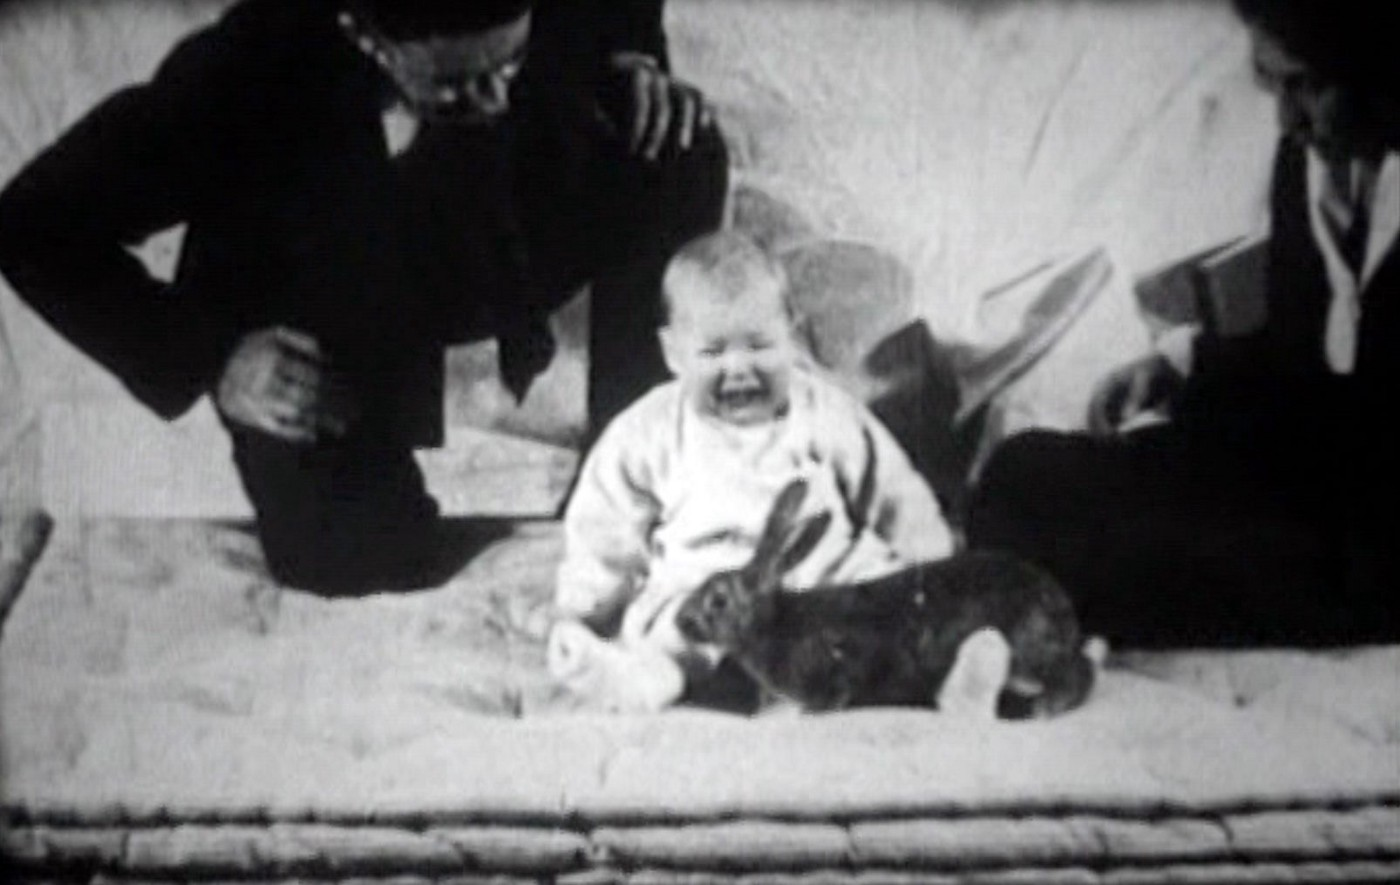
\includegraphics[width=0.95\linewidth]{images/Libro-img002.jpg}
  \begin{minipage}{\linewidth}
    \caption{Un frame estratto dai video girati dal Dr. John Watson e Rosalie Rayner.}
  \end{minipage}
\end{wrapfigure}

Jhon Broadus Watson, nato nel 1878, è conosciuto come il padre del comportamentismo. Voleva dimostrare con un bambino i
cui pattern in risposta agli stimoli sono piuttosto semplici rispetto a un adulto, che si possono indurre, attraverso
il condizionamento ambientale, alcune emozioni come la paura. Albert era un neonato e a 8 mesi e 26 giorni quando
affronta il suo primo test. Uno sperimentatore distrae il bambino, mentre un altro colpisce una sbarra di ferro con un
martello. All'inizio Albert sembra solo spaventato, ma dopo la terza volta che sente il rumore,
scoppia a piangere. Dopo pochi giorni vengono mostrati, ad Albert, un topo bianco, un coniglio, un cane, una scimmia,
maschere, della bambagia, un giornale infuocato e molto altro. Albert non sembra spaventato, siccome non aveva ancora
associato nessuna emozione, positiva o negativa, a queste situazioni. Addirittura prova a toccare la carta infuocata
siccome non ha mai vissuto una scottatura e di conseguenza non ha mai associato il fuoco al dolore. L'esperimento
cercherà di instillare la paura in Albert alla vista di qualcosa che precedentemente non lo spaventava. I ricercatori
hanno deciso di usare il topo bianco, che sembrava incuriosisce Albert. Ogni volta che il bambino provava ad
avvicinarsi al topo, uno sperimentatore colpiva una barra di ferro con un martello. Le prime volte il bambino
sussultava, ma senza piangere. Le volte successive, però, iniziò a piangere. Dopo una settimana Albert era terrorizzato
alla vista del topo e cercava di scappare in lacrime. Successivamente, gli autori scoprono che la risposta condizionata
di paura è stata generalizzata agli altri animali e ad altri oggetti come la pelliccia e, la bambagia. Il
condizionamento si è allargato includendo altri stimoli apparentemente simili al tatto, fino a comprendere i capelli di
Watson e la maschera di Babbo Natale. A questo punto Watson e Rayner tentano il processo inverso per rimuovere queste
paure dal piccolo Albert, ma la madre, trovato un uovo impiego lo allontana dall'esperimento. 

Potete trovare su YouTube i video di questo terrificante esperimento molto
criticato\endnote{\protect\url{https://www.youtube.com/watch?v=FMnhyGozLyE} } condotto nel 1920 dove l'etica
non era un limite così importante ai fini della ricerca scientifica. Gli autori affermarono: “ci sembrava che
l'esperimento potesse arrecare un danno relativamente lieve”. Fortunatamente il piccolo Albert
venne allontanato dalla madre, ma purtroppo morì all'età sei anni di
encefalite.\endnote{\protect\url{https://www.stateofmind.it/2016/01/il-piccolo-albert-esperimento-psicologia/} }
\end{mdframed}

\bigskip

\subsection{Metodo Scientifico}
Siccome tutto ciò che sappiamo sul mondo che ci circonda, su noi stessi, sulle idee che ci siamo fatti, passa attraverso
la mente e la nostra capacità cognitiva è vittima di tante distorsioni, come facciamo ad avere un idea su una
questione?

In aiuto ci viene un metodo, chiamato metodo scientifico. Non mi soffermerò troppo sui vari passaggi che abbiamo
imparato a scuola: osservazione, ricerca, ipotesi, esperimento, analisi ecc… ma del perché sia così efficace. Una
premessa doverosa è specificare che il metodo scientifico non dice cosa è vero e cosa no, infatti escono costantemente
ricerche che invalidano in una certa misura quelle precedenti. Il metodo scientifico dice che ci sono evidenze che
dimostrano un certo fenomeno. Eventualmente dice: questa è la cosa più vera trovata fino a questo momento.

Perché Fidarsi del Metodo Scientifico? 

\begin{itemize}
\item Ripetibilità: La scienza invita alla verifica. Se un esperimento può essere ripetuto con gli stessi risultati,
questo rafforza la fiducia nei suoi risultati.
\item Trasparenza: I metodi e i dati sono aperti, permettendo a chiunque di esaminare e contestare le conclusioni.
\item Falsificabilità: Una teoria scientifica deve poter essere dimostrata falsa. Se non può essere messa alla prova,
non è scienza. 

\begin{itemize}
\item Esempio di teoria falsificabile: “tutti i cigni sono bianchi”. Questa è una teoria che può essere facilmente messa
alla prova: l'osservazione di un solo cigno nero sarebbe sufficiente a falsificarla.
\item Esempio di teoria non falsificabile: “esistono alieni in una galassia lontana 1000 anni luce dalla Terra”. Questa
affermazione non è attualmente testabile con la tecnologia esistente e non c'è modo di progettare
un esperimento che possa confermare o smentire la presenza di vita aliena in quella specifica galassia.
\end{itemize}
\item Peer Review: Prima della pubblicazione, la ricerca è sottoposta a un rigoroso processo di revisione da parte di
esperti anonimi, garantendo che solo il lavoro di alta qualità venga accettato.
\end{itemize}
Quest'ultimo punto in particolare da molta forza al metodo. Abbiamo visto spesso durante gli anni,
anche con la pandemia di Covid 19 che alcuni medici, scienziati, premi nobel possono dire cose contrastanti a quello
che dice la scienza. Questo per i bias che abbiamo visto prima, un singolo scienziato può commettere errori, mentre
diversi ricercatori, di diverse realtà come laboratori o università, se tutti arrivano alle stesse conclusioni con gli
stessi esperimenti, abbattono notevolmente l'errore umano. Inoltre, durante il processo di
pubblicazione su una rivista scientifica, i ricercatori restano anonimi a chi dovrà valutare lo studio e viceversa,
questo per evitare pregiudizi o anche solo interessi economici che possano corrompere qualcuno nei vari step che
porteranno alla pubblicazione dell'articolo.

Quindi la scienza non ha bias?

No, anche la scienza li ha, facciamo un esempio: Uno studio intende valutare l'efficacia di un
programma di perdita di peso per persone con diabete. Se lo studio si concentra solo sul numero di partecipanti che
completano il programma senza considerare altri fattori, come il tasso di abbandono o i cambiamenti nel comportamento
alimentare, potrebbe portare a conclusioni distorte. Ad esempio, se i partecipanti che non perdono peso tendono ad
abbandonare il programma e vengono così esclusi dai risultati, mentre quelli che hanno successo continuano, i risultati
potrebbero essere sbilanciati verso esiti più favorevoli.

Un altro esempio potrebbe essere uno studio sull'uso degli smartphone e i sintomi
muscoloscheletrici tra gli studenti delle scuole superiori. Se lo studio si basa su dati auto-segnalati dagli studenti
senza verificare l'accuratezza di tali dati, potrebbe esserci un bias informativo. Gli studenti
potrebbero sovrastimare o sottostimare il tempo trascorso al telefono, influenzando così i risultati dello studio.

Quindi come facciamo a sapere se una ricerca è affidabile? Soprattutto quando andiamo a leggere di una materia di cui
non abbiamo competenze?

Per prima cosa cerchiamo un articolo scientifico e per farlo possiamo affidarci a Google Scholar, fatto da Google e con
il medesimo funzionamento: \protect\url{https://scholar.google.com}

Una volta fatta la ricerca, sulla colonna di sinistra, clicchiamo su “Articoli scientifici”.

I primi risultati sono i più pertinenti, e una volta scelto l'articolo che ci interessa esaminiamo
la rivista. Riviste con un rigoroso processo di revisione paritaria sono generalmente considerate più affidabili, ma
questo può essere complicato da valutare anche con delle ricerche su Google per un non addetto ai lavori. Esiste un
indice che ci aiuta in questa analisi che è l'Impact Factor (IF). Questo indice riflette la media
annuale delle citazioni degli articoli pubblicati negli ultimi due anni in una determinata rivista, ed spesso
utilizzato come un indicatore dell'importanza relativa di una rivista nel suo campo; le riviste
con valori IF più alti sono considerate più importanti o prestigiose e potete trovarli su questo sito:
\ \protect\url{https://exaly.com/journals/if/}

Esistono diversi indicatori alternativi all'Impact Factor per valutare l'importanza e l'influenza di una rivista
scientifica. Ecco alcuni dei più noti:

\begin{itemize}
\item \begin{itemize}
\item SCImago Journal Rank (SJR): Utilizza dati provenienti da Scopus e considera sia il numero di citazioni ricevute
che la prestigio delle riviste da cui provengono le citazioni. \protect\url{https://www.scimagojr.com/journalrank.php} 
\item CiteScore: Calcolato anch'esso su dati Scopus, rappresenta il numero medio di citazioni ricevute in un anno da
articoli pubblicati nei tre anni precedenti.
\item Source Normalized Impact per Paper (SNIP): Misura l'impatto contestualizzato di una rivista, tenendo conto delle
caratteristiche del campo di ricerca.
\item Eigenfactor Score: Basato sul numero di volte in cui gli articoli della rivista sono stati citati negli ultimi
cinque anni, ma anche sulla {\textquotedbl}qualità{\textquotedbl} delle citazioni ricevute.
\end{itemize}
\end{itemize}

\bigskip

Non avendo competenze per valutare autonomamente uno studio, dobbiamo delegare questa responsabilità alla rivista
scientifica che sceglieremo tramite l'impact score, un indice basato sulle citazioni. Questo indice ci indica che
esperti capaci di fare tale valutazione hanno citato tali studi nelle loro ricerche, considerandoli validi. Questo
controllo quindi potrebbe essere sufficiente, in quanto, valutata la serietà di una rivista, anche i punti che vedremmo
in seguito, saranno già stati valutati. Un altro controllo molto veloce e che aumenta di molto la credibilità di uno
studio è vedere quante volte l'articolo è stato citato da altre ricerche. Se un articolo è stato
citato molto volte in altre ricerche vuol dire che persone competenti in quella materia hanno ritenuto valido questo
studio, analizzandolo, meglio di come potremmo fare noi outsider. Potete vedere le citazioni in Google Scholar, già dai
risultati di ricerca, prima ancora di entrare dentro l'articolo vero e proprio.


\bigskip

Per i più scrupolosi di voi, si può valutare una ricerca anche con i seguenti punti:


\bigskip

\begin{itemize}
\item Ricerca di conflitti di interesse: Solitamente in fondo alla ricerca vengono citati anche i finanziatori. Se una
ricerca mette in luce i benefici di un certo integratore e tra i finanziatori, con una semplice ricerca vediamo che le
persone o le aziende in questione producono quegli integratori possiamo dire che è piuttosto sospetta.
\item Verifica gli autori: Controlla le qualifiche degli autori e la loro affiliazione istituzionale. Gli autori
rispettabili e le istituzioni rinomate possono aumentare la credibilità della ricerca.
\item Controlla le citazioni: Uno studio che cita fonti pertinenti e attuali dimostra che gli autori hanno considerato
il contesto della loro ricerca.
\item Analizza i dati e i risultati: I risultati dovrebbero essere presentati in modo chiaro e supportati dai dati.
Attenzione a qualsiasi affermazione che sembra troppo buona per essere vera o non supportata da prove.
\item Consulta esperti: Se possibile, discuti la ricerca con colleghi o esperti nel campo per ottenere la loro opinione
sulla validità dello studio.
\end{itemize}

\bigskip

Noterai subito che gli articoli scientifici sono numerosi e in continuo aumento di anno in anno, come posso leggere così
tante pagine per ogni dubbio che ho? La scienza sta diventando sempre più accessibile, infatti gli articoli sono
strutturati in modo da mettere all'inizio un abstract, che solitamente è fatto da pochi paragrafi,
che sostanzialmente è un riassunto. Negli ultimi anni sempre più articoli inseriscono gli highlights, che sono i punti
principali, per renderci ancora più facile e veloce avere un idea di massima di cosa parla
l'articolo.


\bigskip

Meglio ancora degli articoli scientifici ci sono le meta-analisi scientifiche, un tipo di revisione sistematica che
combina i risultati di diversi studi indipendenti su una stessa domanda di ricerca. Questo processo statistico valuta
l'efficacia clinica calcolando una stima combinata ponderata degli interventi, basata su almeno
due studi separati. Le meta-analisi sono strumenti potenti che possono migliorare la precisione, risolvere controversie
derivanti da risultati contrastanti e rispondere a domande che non possono essere affrontate da singoli studi. Inoltre,
aiutano a standardizzare e migliorare la qualità delle revisioni sistematiche attraverso linee guida come la
dichiarazione PRISMA.

Quindi se leggete un articolo su internet che parla di ricerche, controllate se avete gli estremi di questo articolo in
modo che possiate analizzarlo. In modo da poter essere critici anche quando si parla di numeri e grafici. Un libro che
mi ha aiutato a capire quanto anche i numeri possano mentire è stato
Factfulness\endnote{\protect\url{https://www.amazon.it/dp/B07BMN2N6D/ref=dp-kindle-redirect?\_encoding=UTF8\&btkr=1},} dove anche
valori corretti, se elaborarli o visualizzati in un certo modo, possono far assumere un concetto molto diverso.

\begin{figure}[H]
    \begin{minipage}{0.3\textwidth}
        \centering
        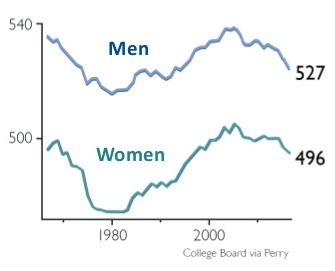
\includegraphics[width=\linewidth]{images/Libro-img003.jpg}
    \end{minipage}
    \hfill
    \begin{minipage}{0.3\textwidth}
        \centering
        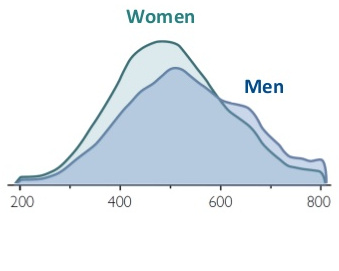
\includegraphics[width=\linewidth]{images/Libro-img004.jpg}
    \end{minipage}
    \hfill
    \begin{minipage}{0.3\textwidth}
        \centering
        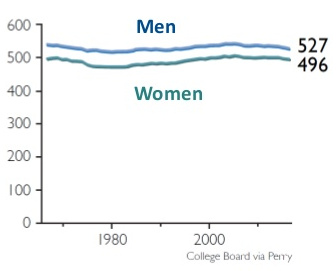
\includegraphics[width=\linewidth]{images/Libro-img005.jpg}
    \end{minipage}
\end{figure}

Questi tre grafici che ritroviamo sul libro mostrano i risultati di test di matematica divisi tra uomini e donne. Se
guardiamo il primo grafico, dove sono mostrate le medie dei test di matematica nei vari anni, vediamo che le donne
conseguono un punteggio decisamente inferiore rispetto agli uomini, ma è davvero così? Spostiamoci sul secondo grafico,
i dati sono gli stessi, ma mostrando sull'asse Y i valori da 0 a 600, rispetto al primo grafico
dove erano da 450 a 540, la differenza di punteggio in campo matematico tra i due sessi sembra decisamente inferiore
ora. Factfulness spiega come le medie possano essere fuorvianti. I primi due grafici mostrano i risultati medi di ogni
anno, mentre nel terzo vediamo tutti i risultati, senza medie, di un solo anno, il 2016. Notiamo come i dati sono quasi
sovrapponibili, non mostrando significative differenze tra uomini e donne.

Quando una storia parla di un divario, creando due gruppi separati con uno spazio nel mezzo, fate attenzione! Spesso la
realtà non è polarizzata, non c'è bianco o nero, ma una grande zona grigia. Fate attenzione alle
medie e cercate le dispersioni, potrebbero sovrapporsi e non mostrare le differenze indicate dalle medie. Riconoscete
quando vengono confrontati due estremi, di gruppi, paesi, persone, sesso, ecc… ci saranno sempre elementi in cima e in
fondo, ma la verità sta nel mezzo, dove c'è la maggioranza.

Questo libro inoltre, in controtendenza con l'idea condivisa che il mondo sta lentamente andando in
rovina, mostra in realtà una tendenza contraria. Alcuni ricercatori come Max Roser, dell'Università di Oxford tramite
ourworldindata.org, Anna Rosling Rönnlund, Hans Rosling e Ola Rosling, ci mostrano anni di dati che danno una visione
del mondo molto più ottimistica sotto vari punti di vista. Vediamone alcuni:

\begin{table}[H]
\centering
\begin{tabular}{cc}
  \begin{subfigure}{0.5\textwidth}
    \centering
    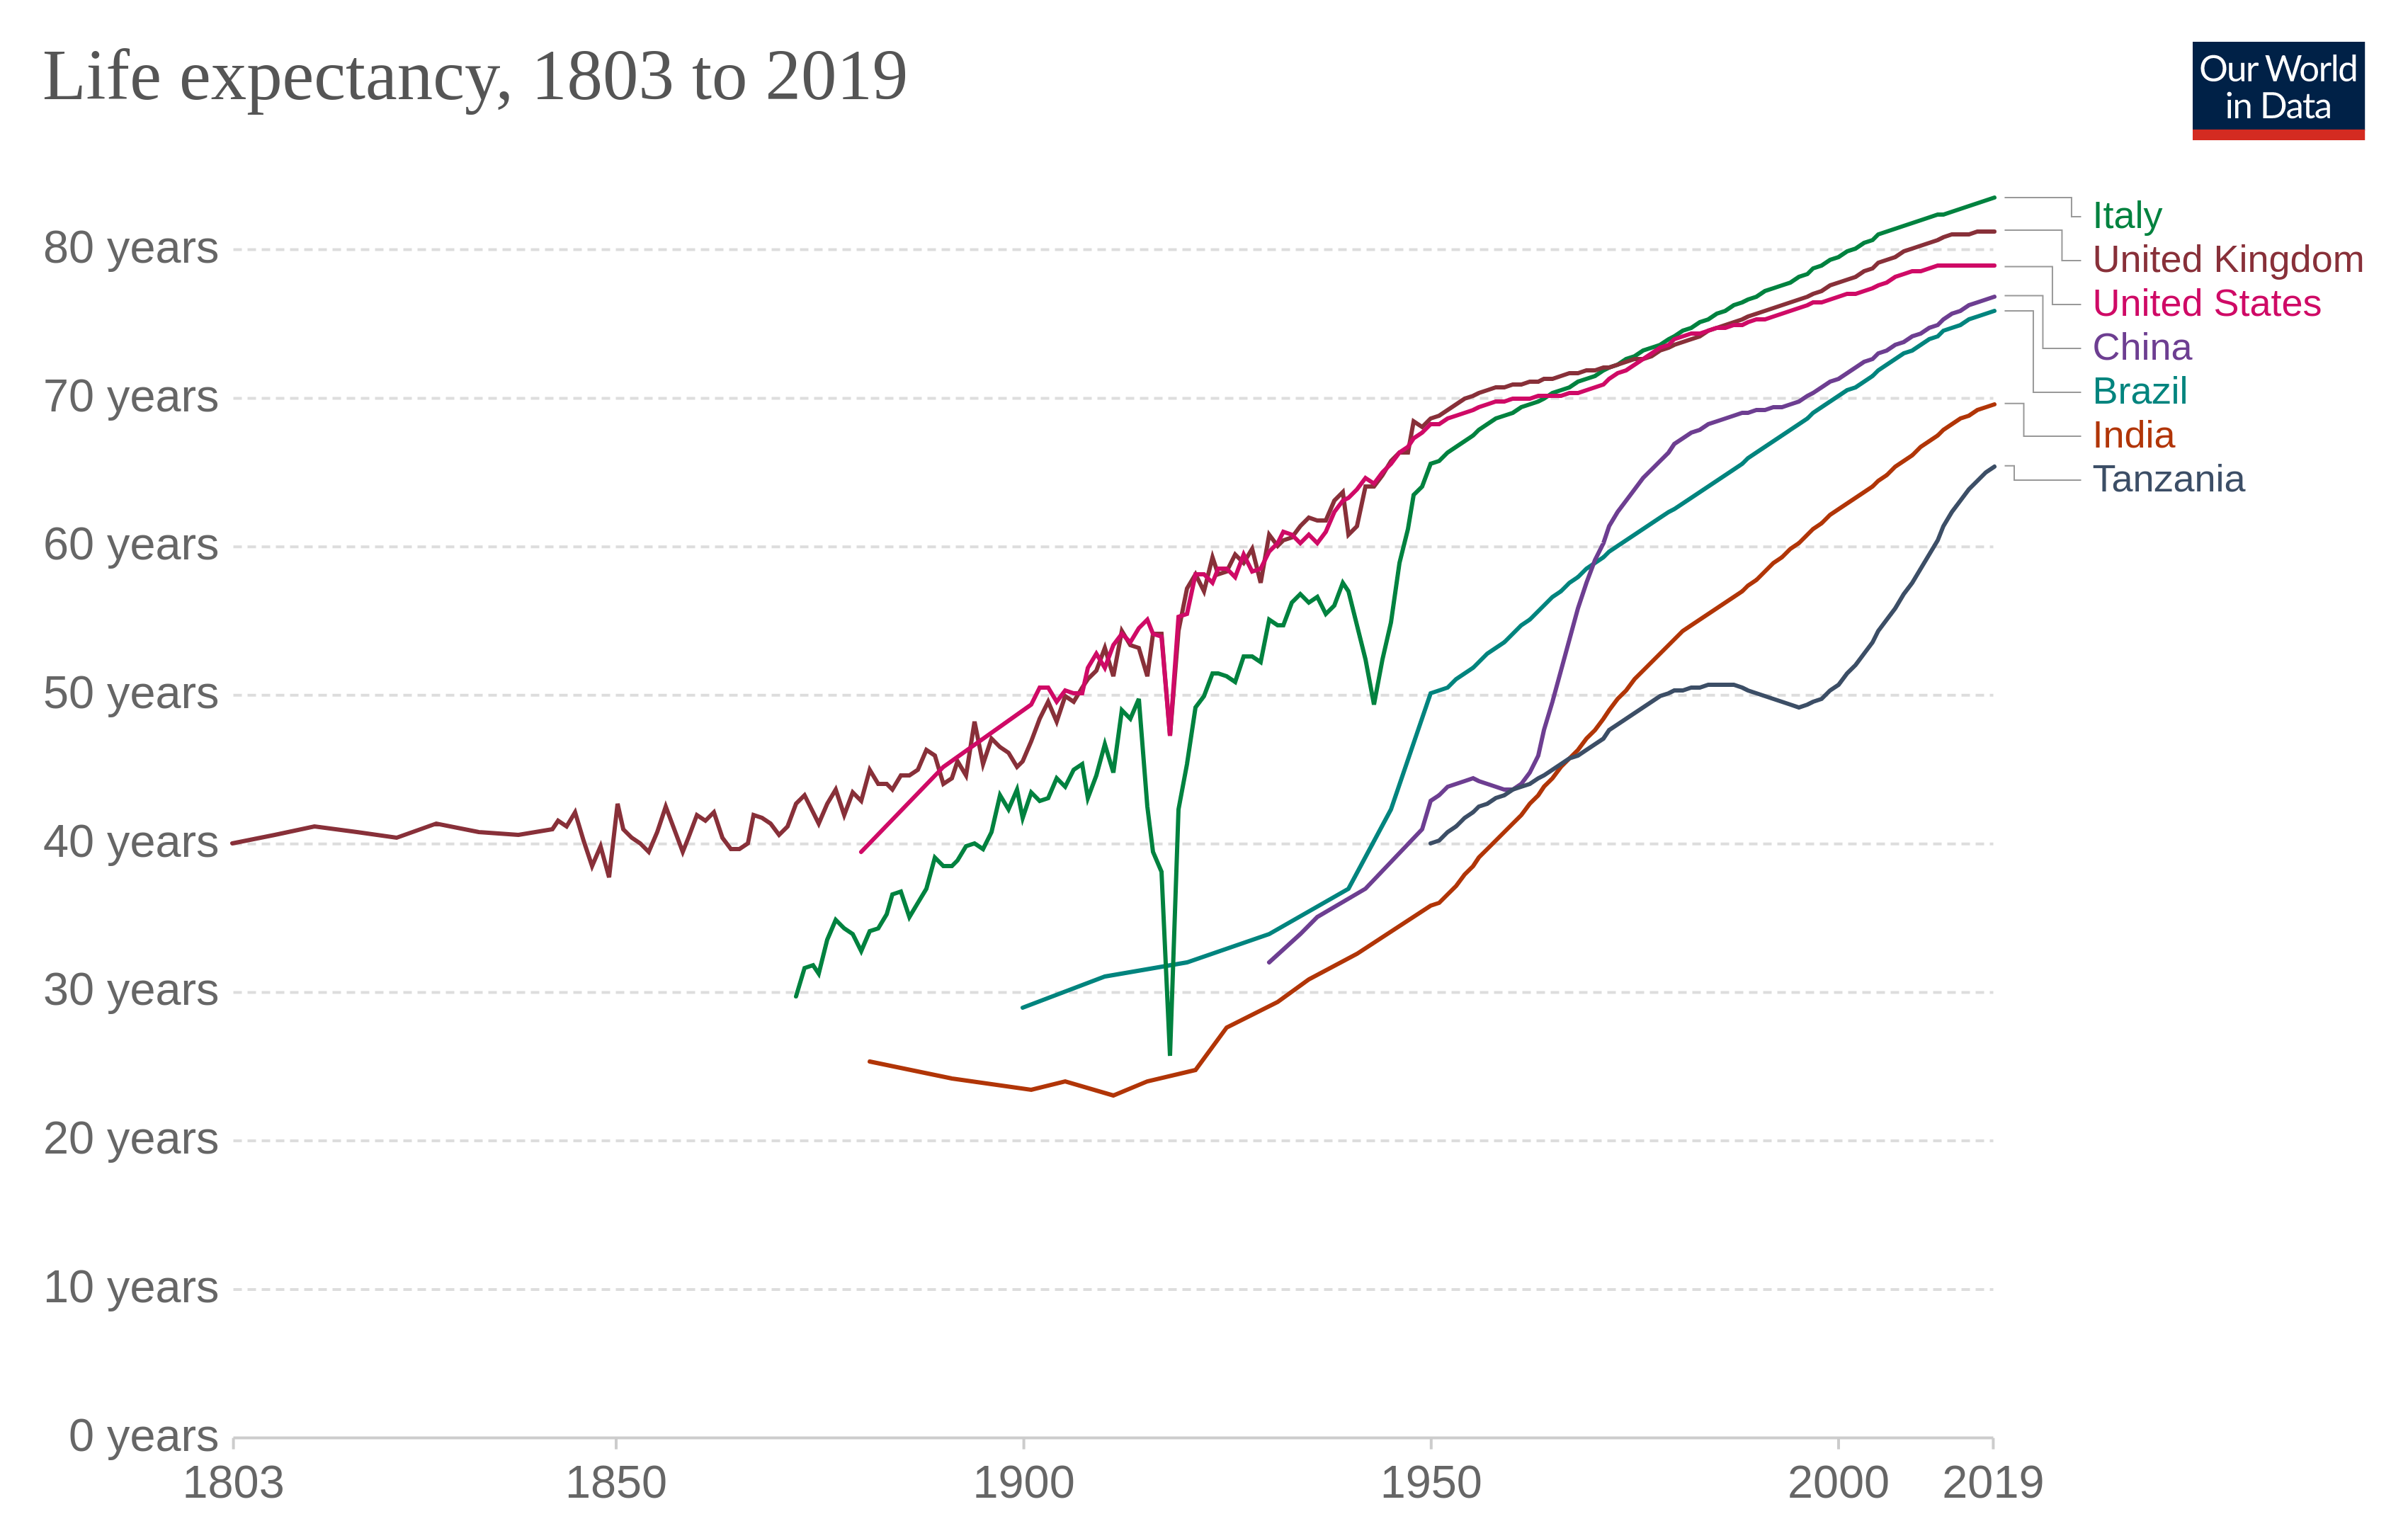
\includegraphics[width=0.8\linewidth]{images/Libro-img006.png}
    \caption{L'aspettativa di vita è raddoppiata dal 1800 al 2011
Credits: \protect\url{https://ourworldindata.org/grapher/life-expectancy?country=BRA+CHN+IND+TZA+GBR+USA} Source: Riley (2005), Clio
Infra (2015), and UN Population Division (2019) OurWorldInData.org/life-expectancy • CC BY}
  \end{subfigure}
  &
  \begin{subfigure}{0.5\textwidth}
    \centering
    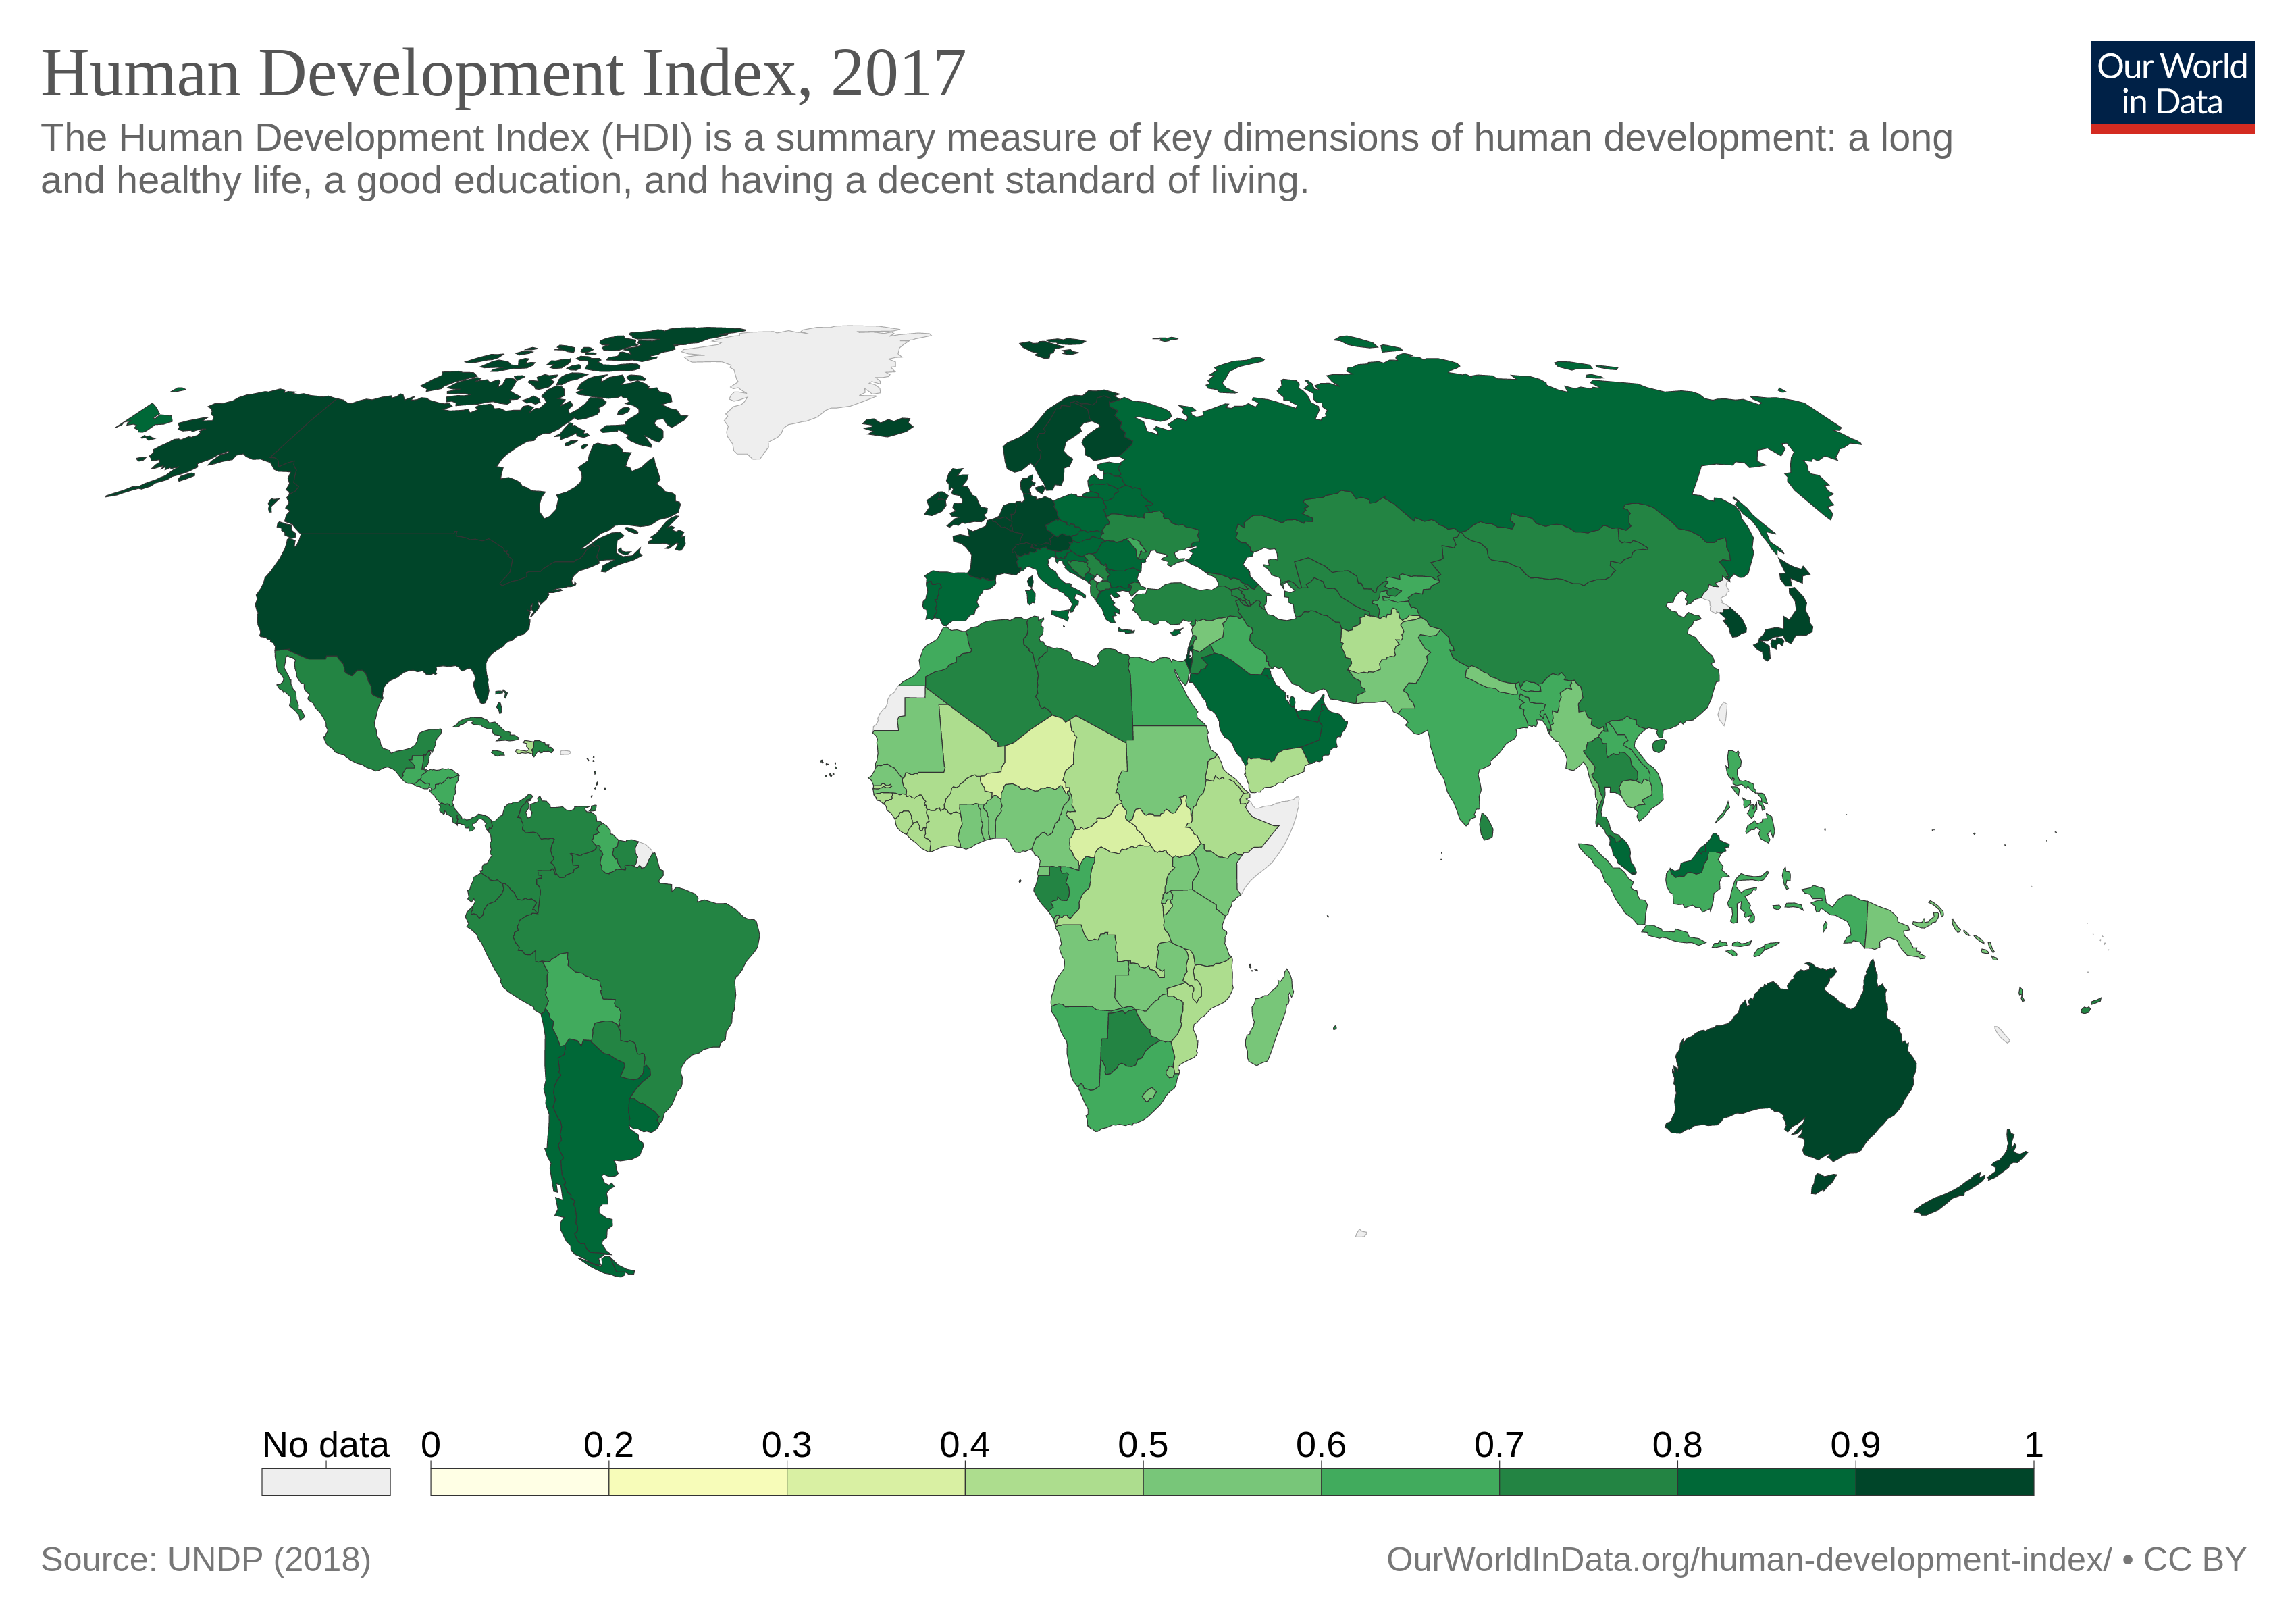
\includegraphics[width=0.8\linewidth]{images/Libro-img007.png}
    \caption{L'indice dello sviluppo umano (HDI) delle nazioni unite è in continua crescita, meno del 10\% delle
persone sulla terra vive in condizioni di povertà assoluta (nel 1900 era l'80\%)
Credits: \protect\url{https://ourworldindata.org/grapher/human-development-index?year=earliest}}
  \end{subfigure}
\end{tabular}
\end{table}

\begin{table}[H]
\centering
\begin{tabular}{cc}
  \begin{subfigure}{0.5\textwidth}
    \centering
    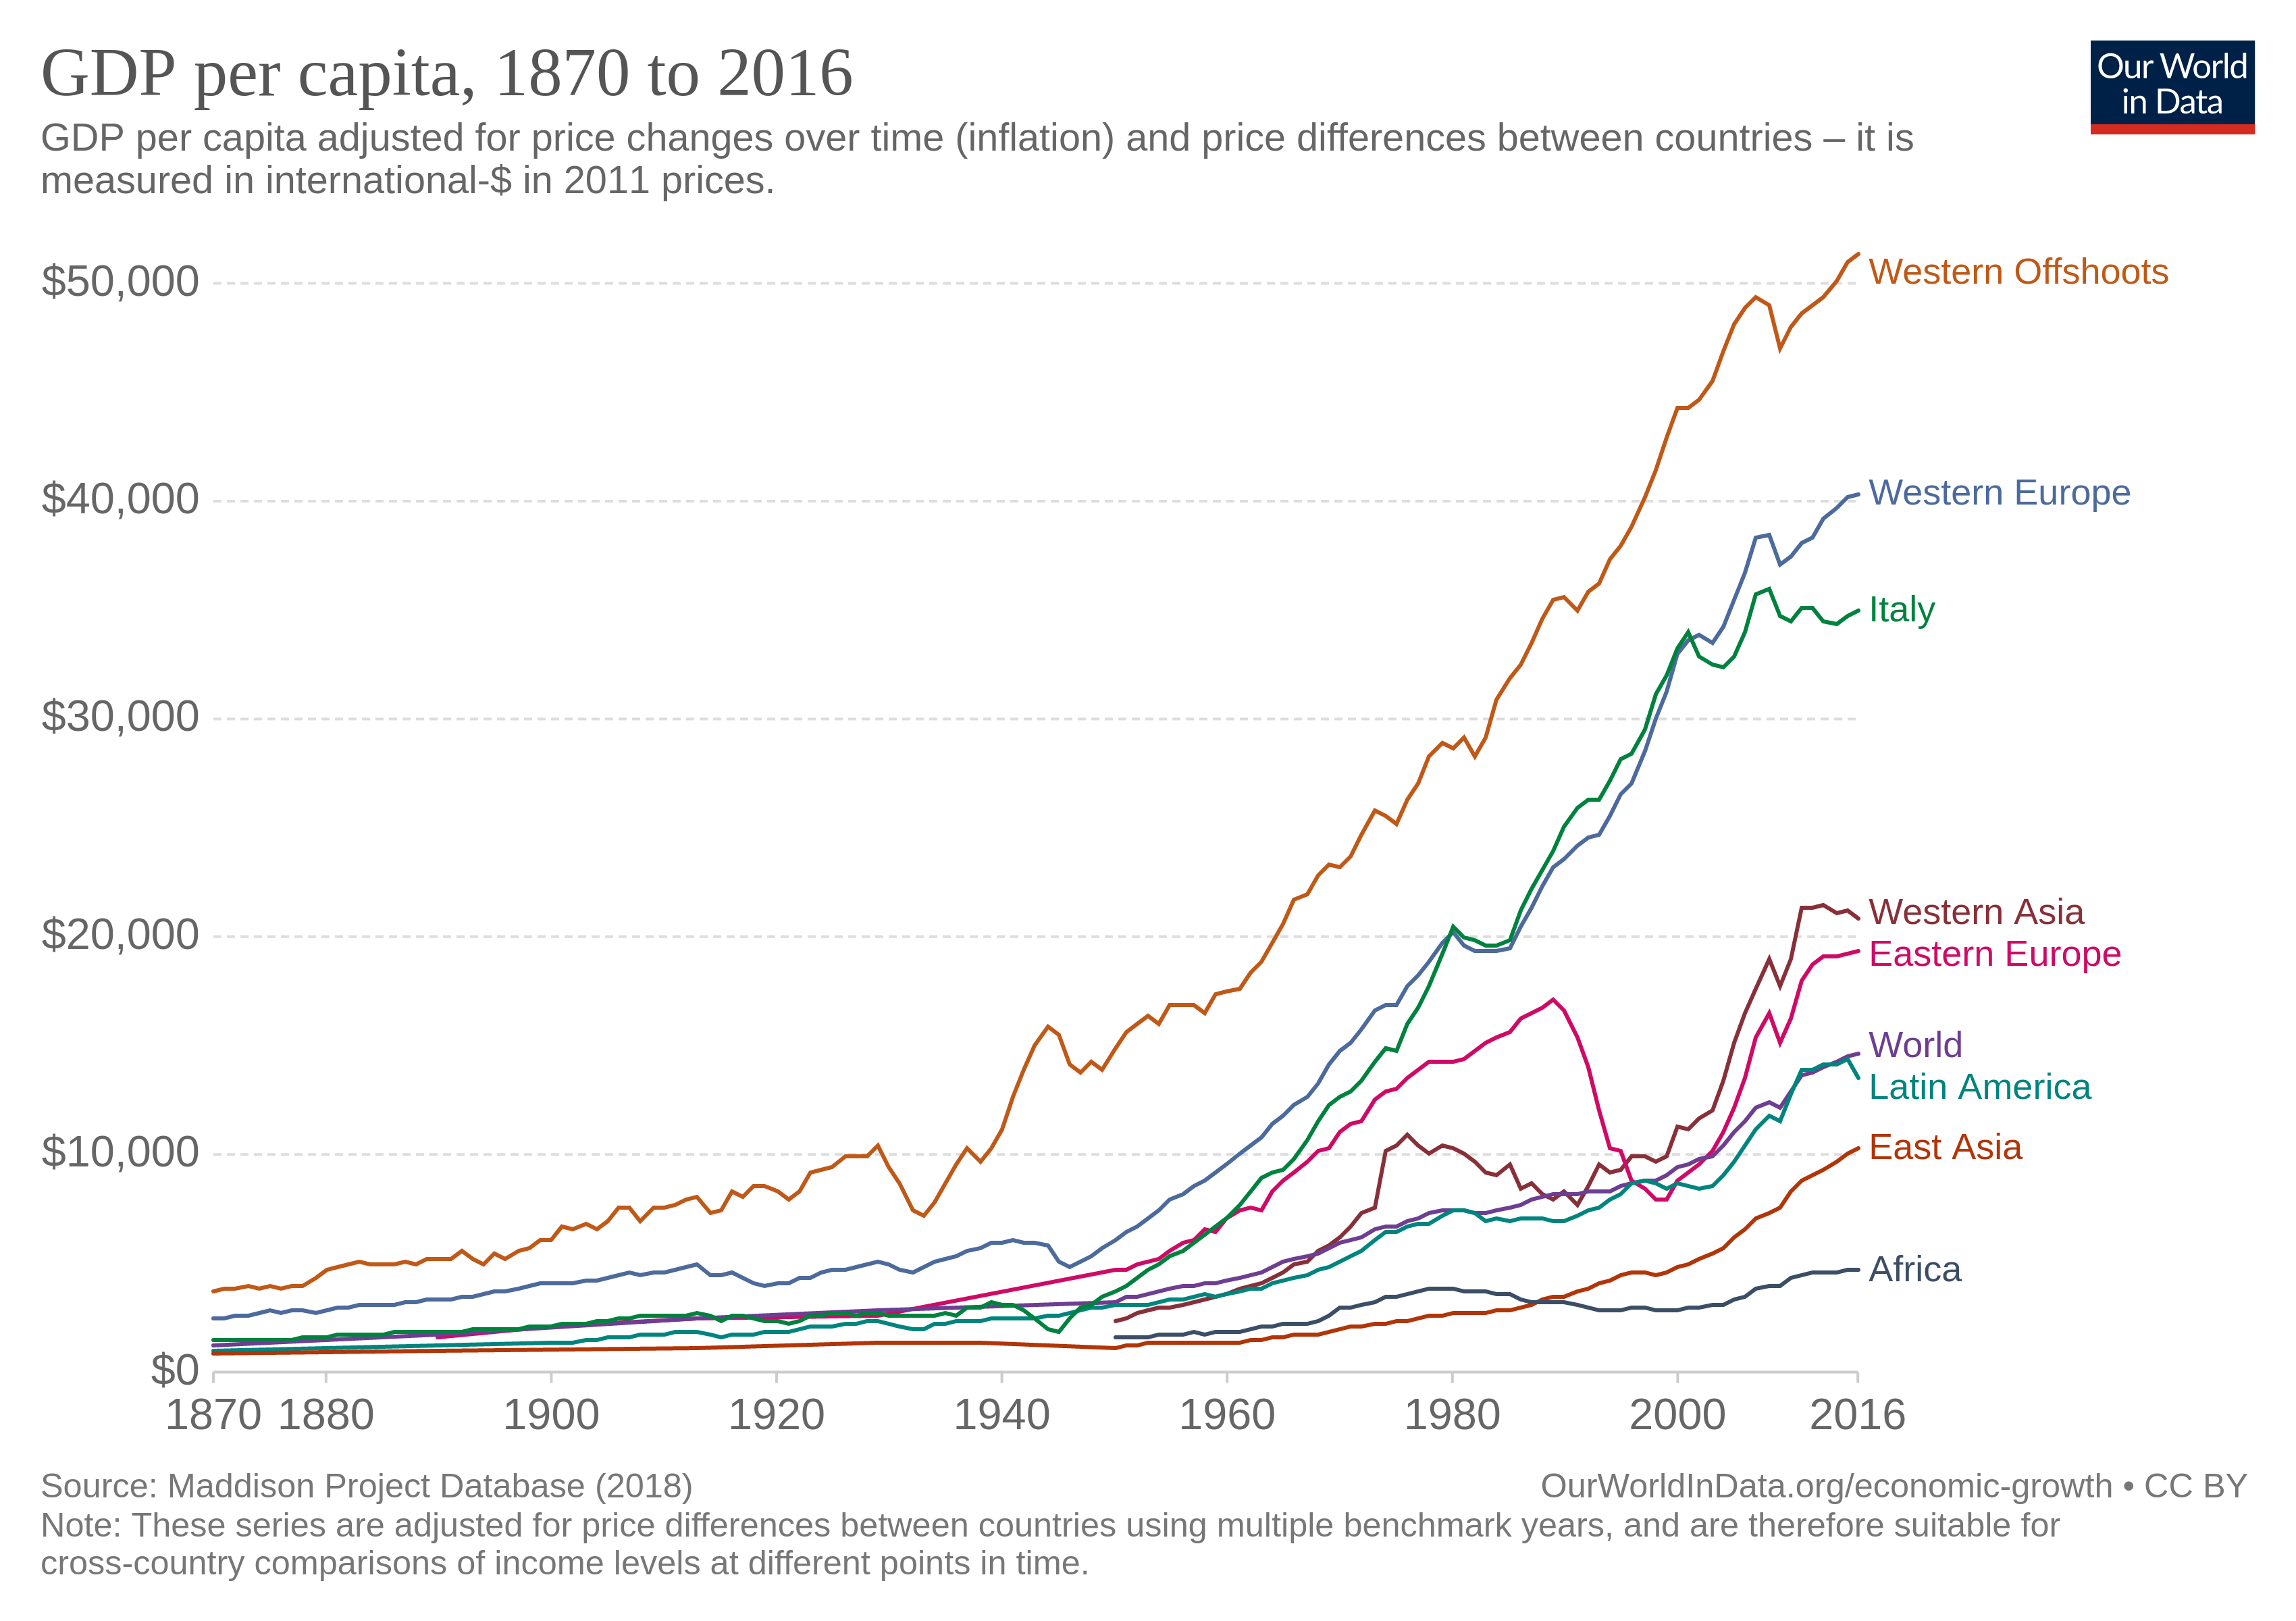
\includegraphics[width=0.8\linewidth]{images/Libro-img008.png}
    \caption{Il PIL è in continuo aumento
Credits: \protect\url{https://ourworldindata.org/grapher/average-real-gdp-per-capita-across-countries-and-regions}}
  \end{subfigure}
  &
  \begin{subfigure}{0.5\textwidth}
    \centering
    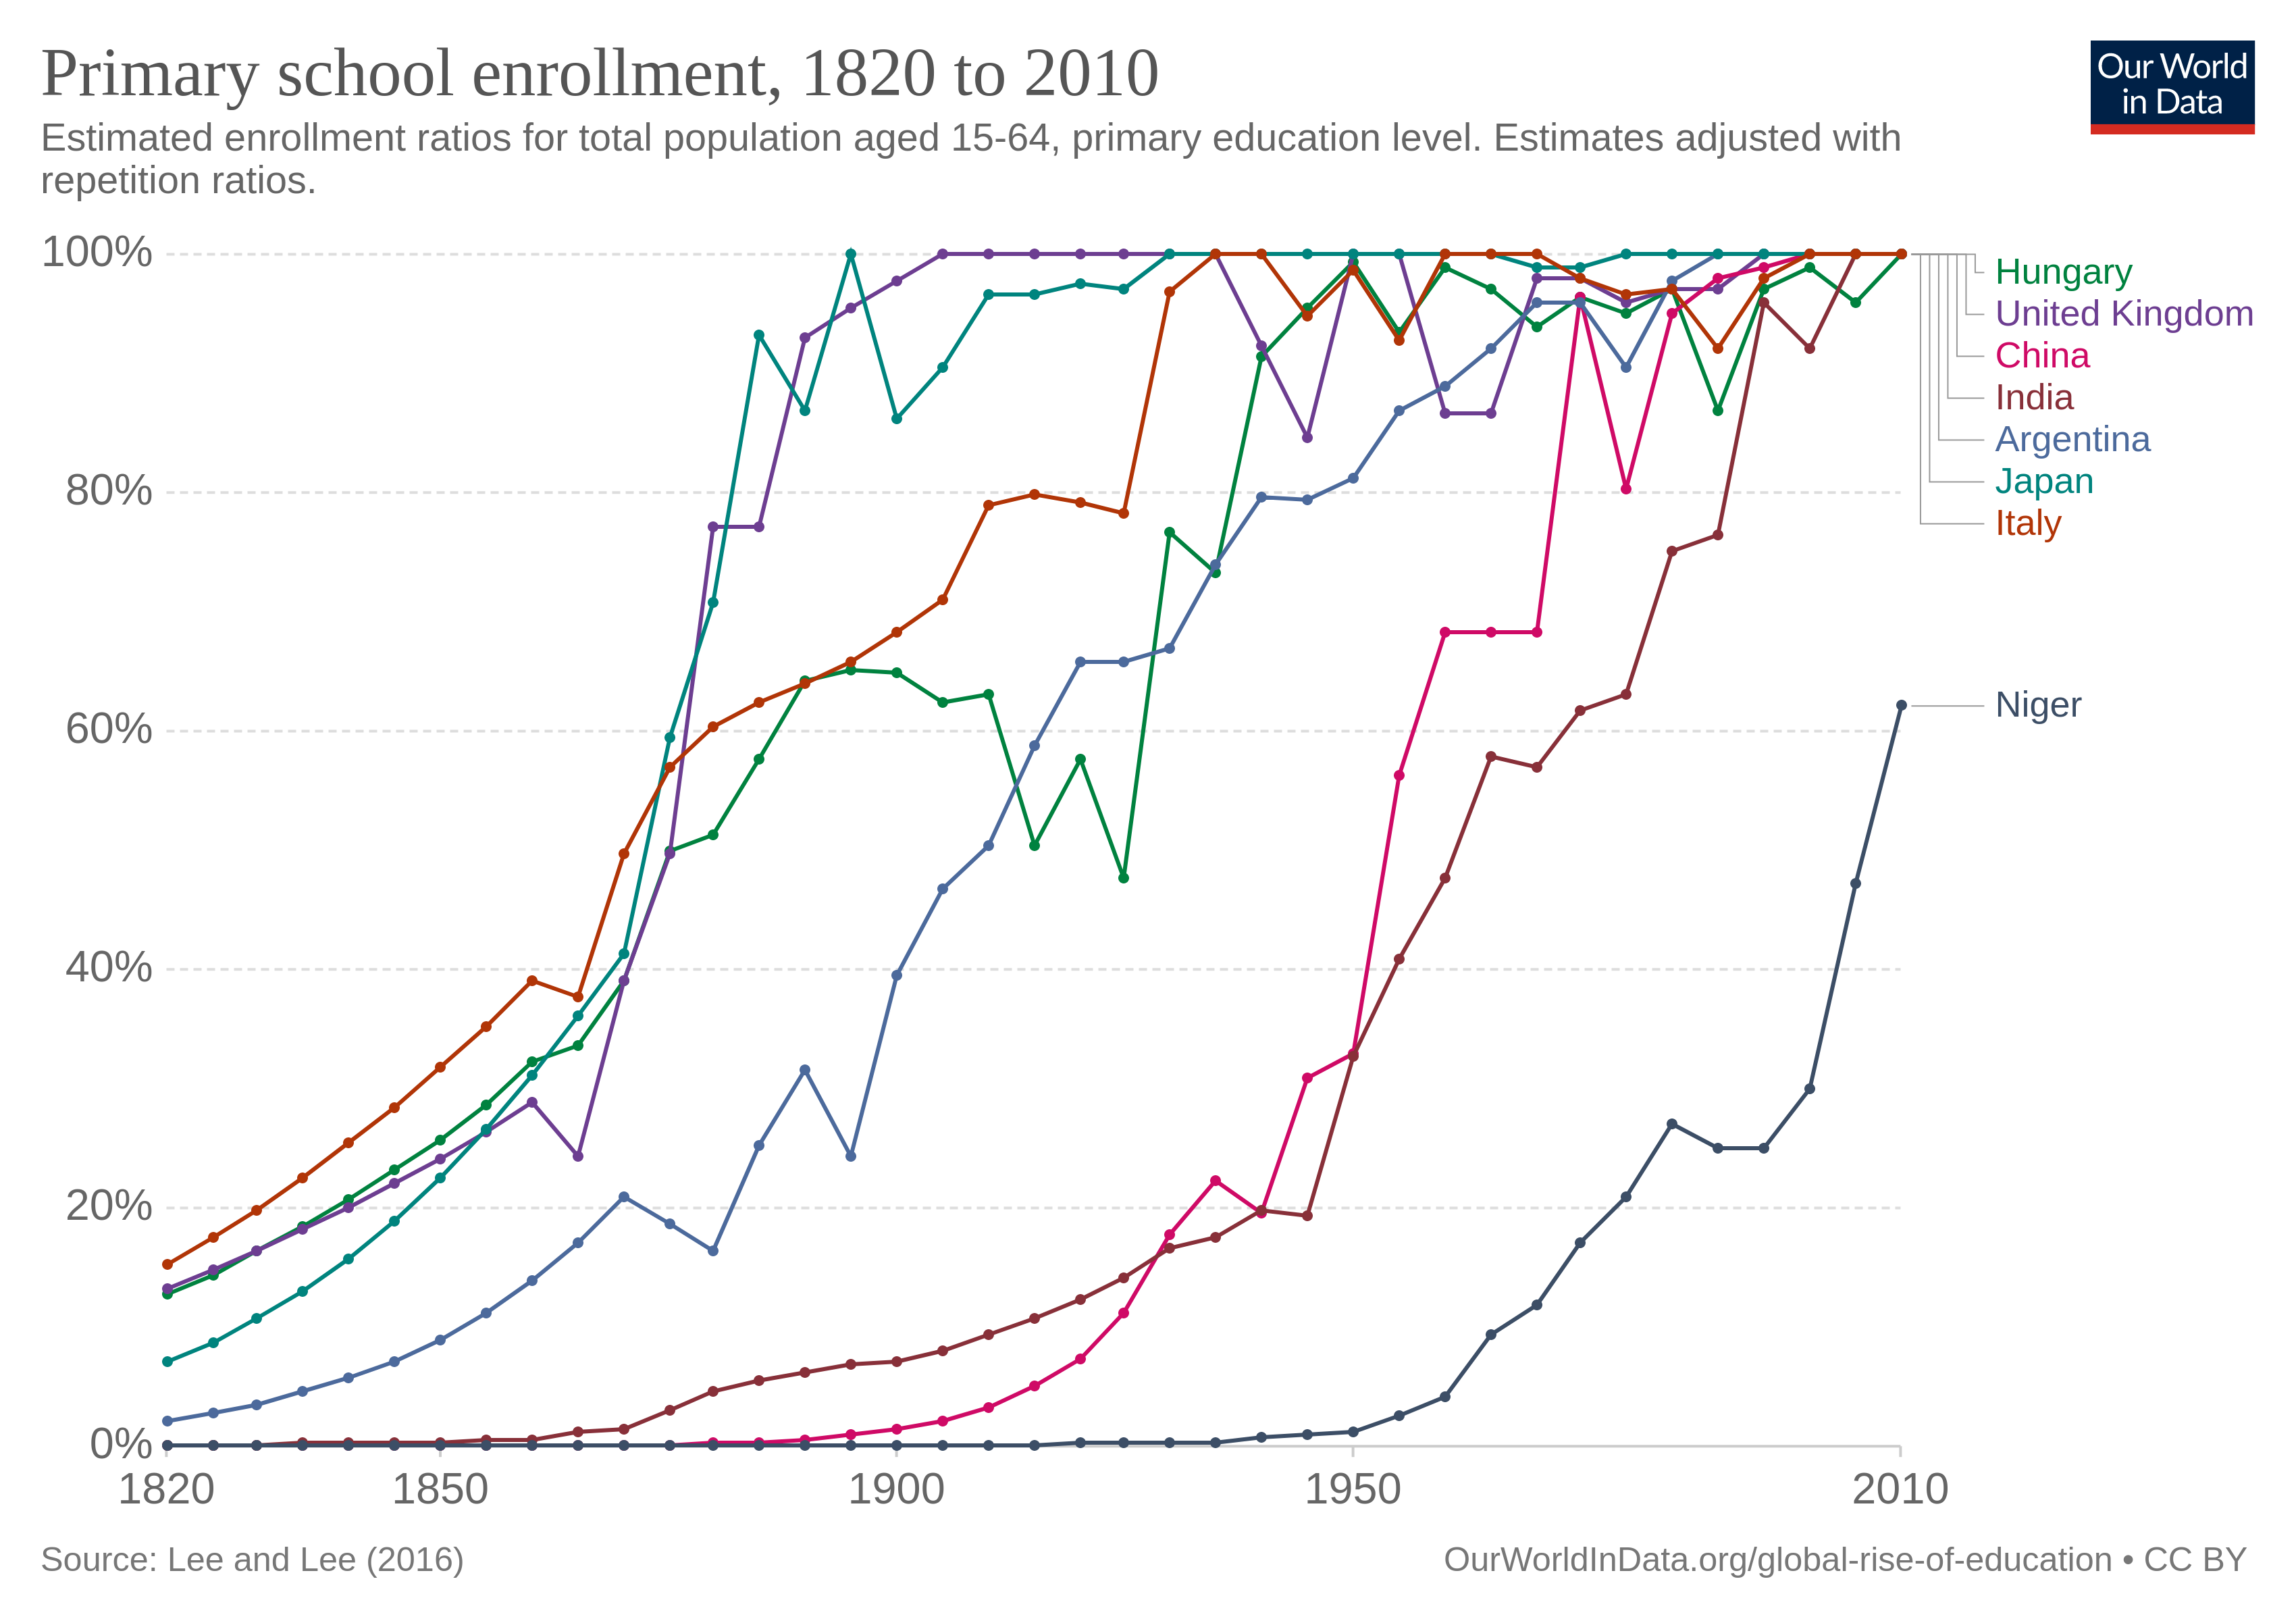
\includegraphics[width=0.8\linewidth]{images/Libro-img009.png}
    \caption{Migliora la ridistribuzione della ricchezza e il conseguente aumento dell'istruzione
Credits : \protect\url{https://ourworldindata.org/global-education\#school-enrollment-and-attendance}}
  \end{subfigure}
\end{tabular}
\end{table}

\begin{table}[H]
\centering
\begin{tabular}{cc}
  \begin{subfigure}{0.5\textwidth}
    \centering
    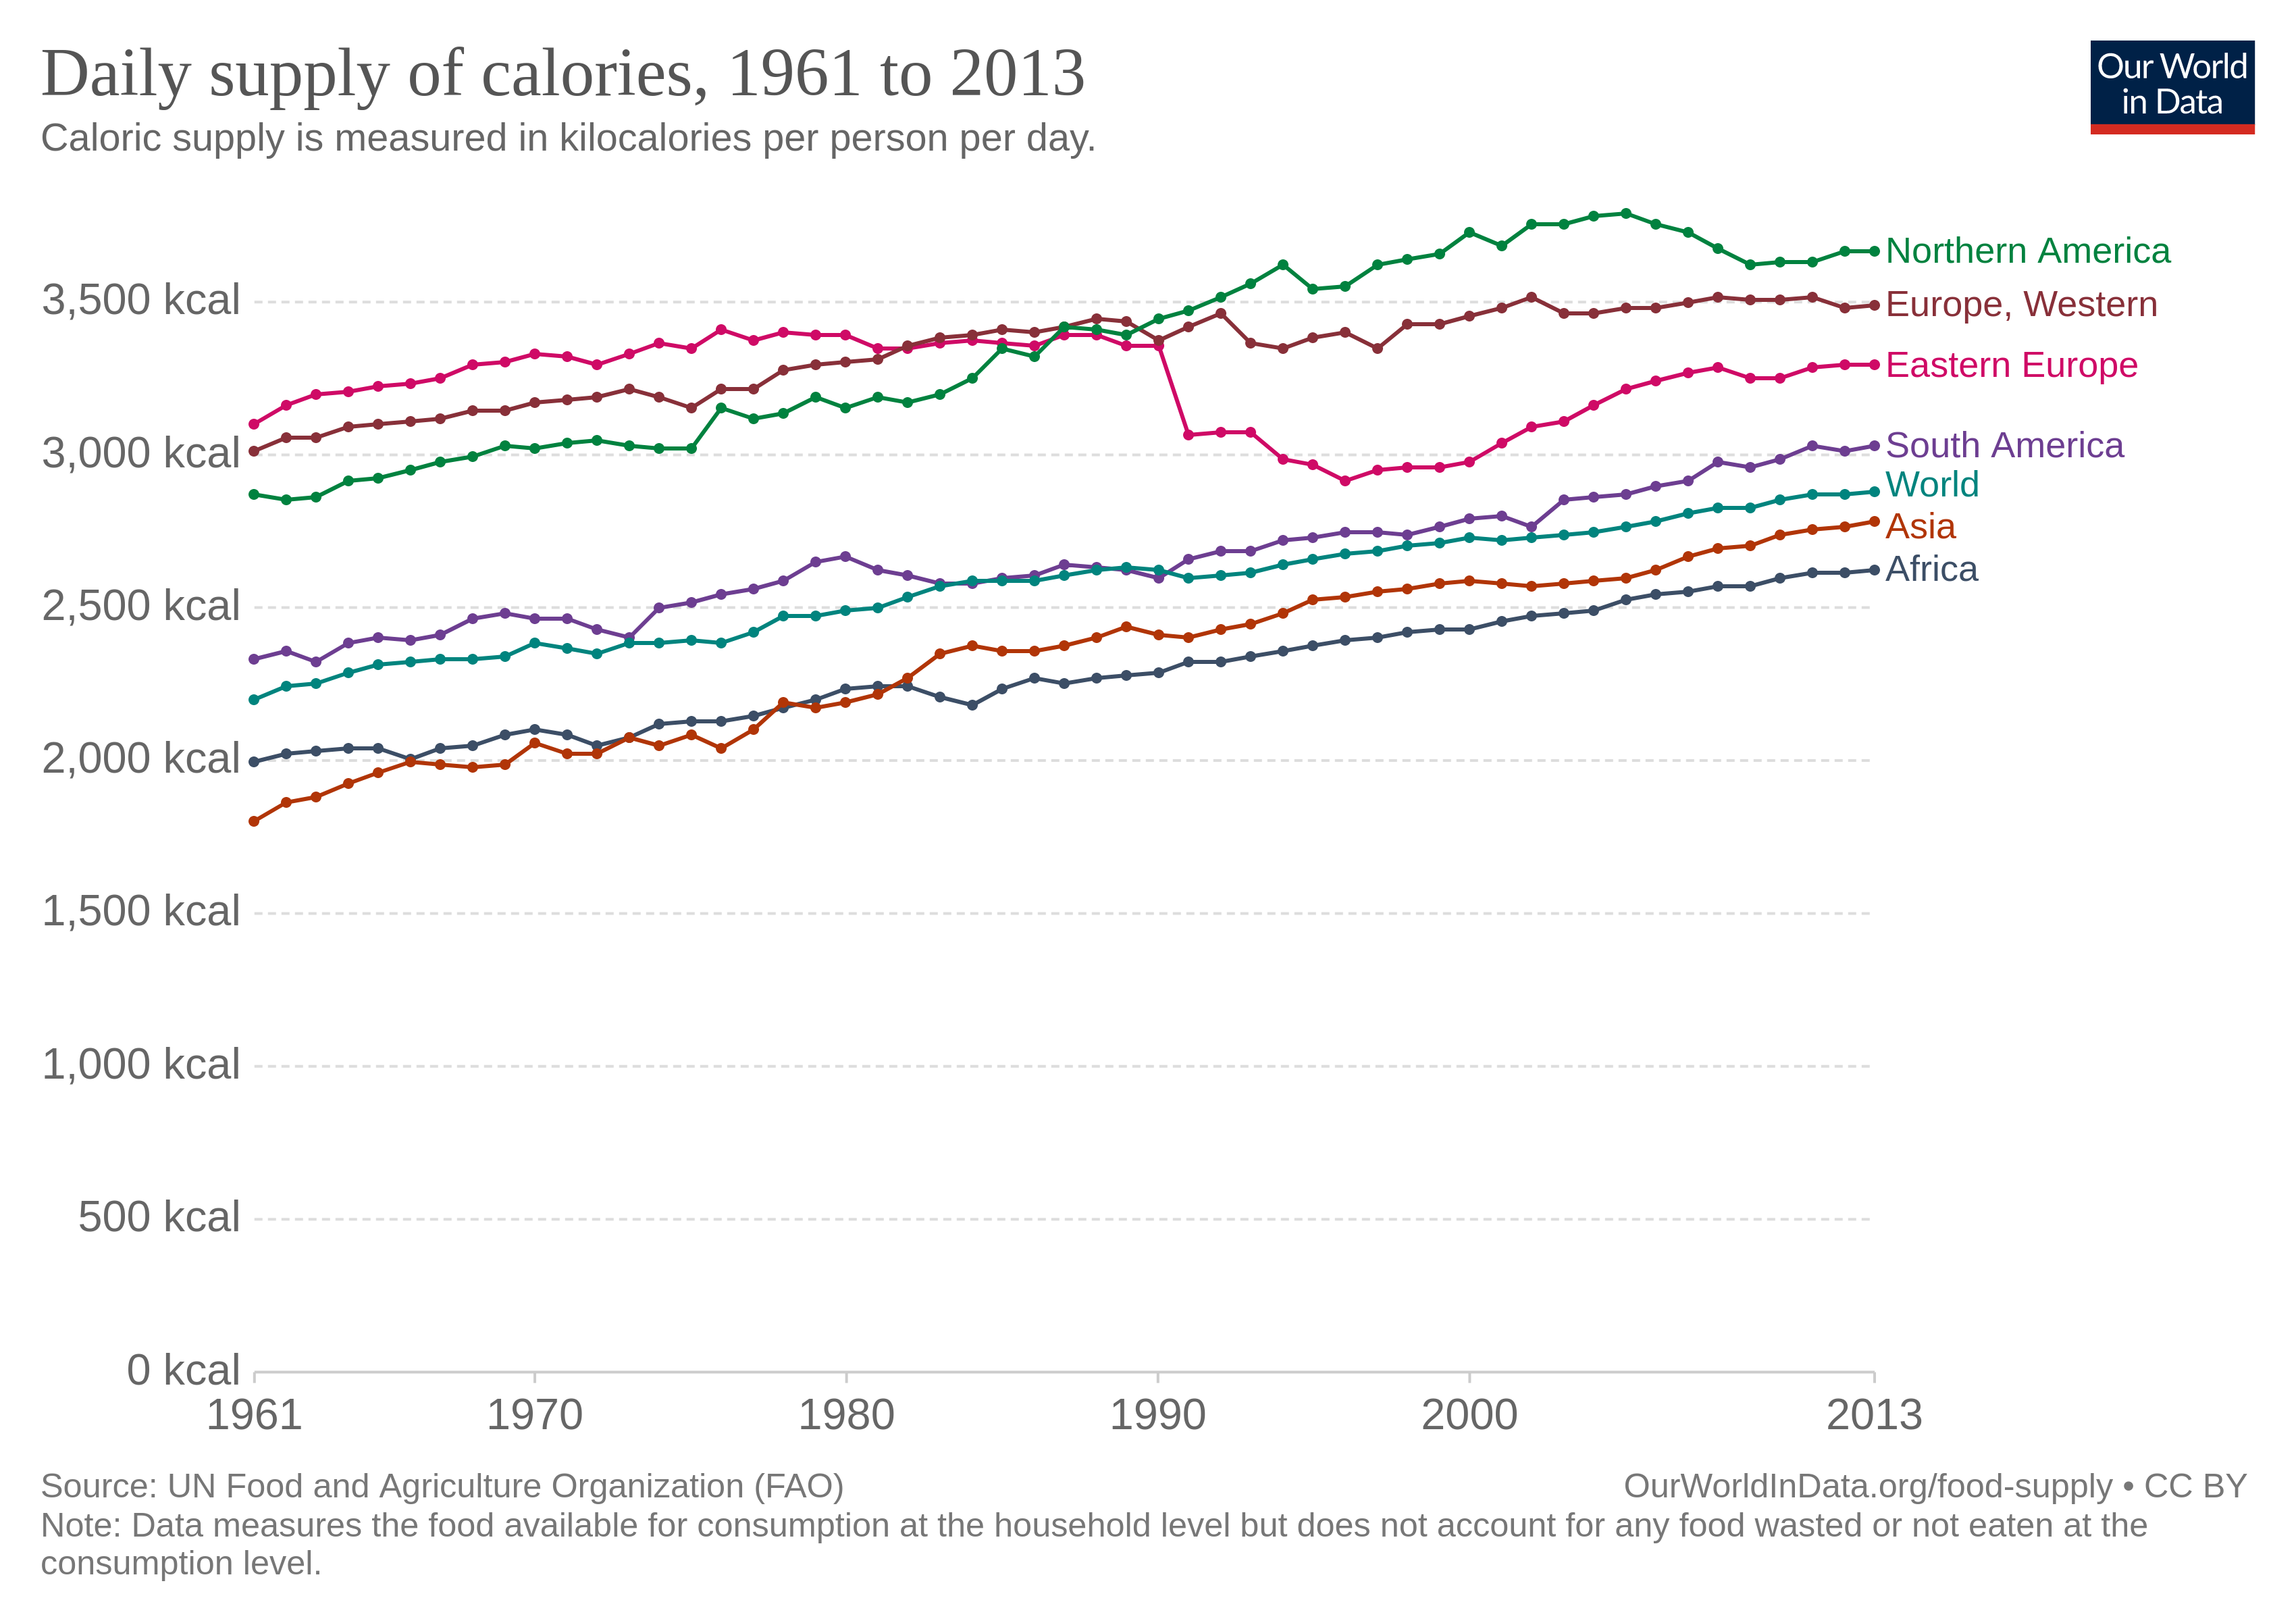
\includegraphics[width=0.8\linewidth]{images/Libro-img010.png}
    \caption{Aumenta la quantità di cibo prodotto
Credits: \protect\url{https://ourworldindata.org/wp-content/uploads/datamaps/kcalPerCapita\_since1961\_FAO/kcalPerCapita\_since1961\_FAO.html}}
  \end{subfigure}
  &
  \begin{subfigure}{0.5\textwidth}
    \centering
    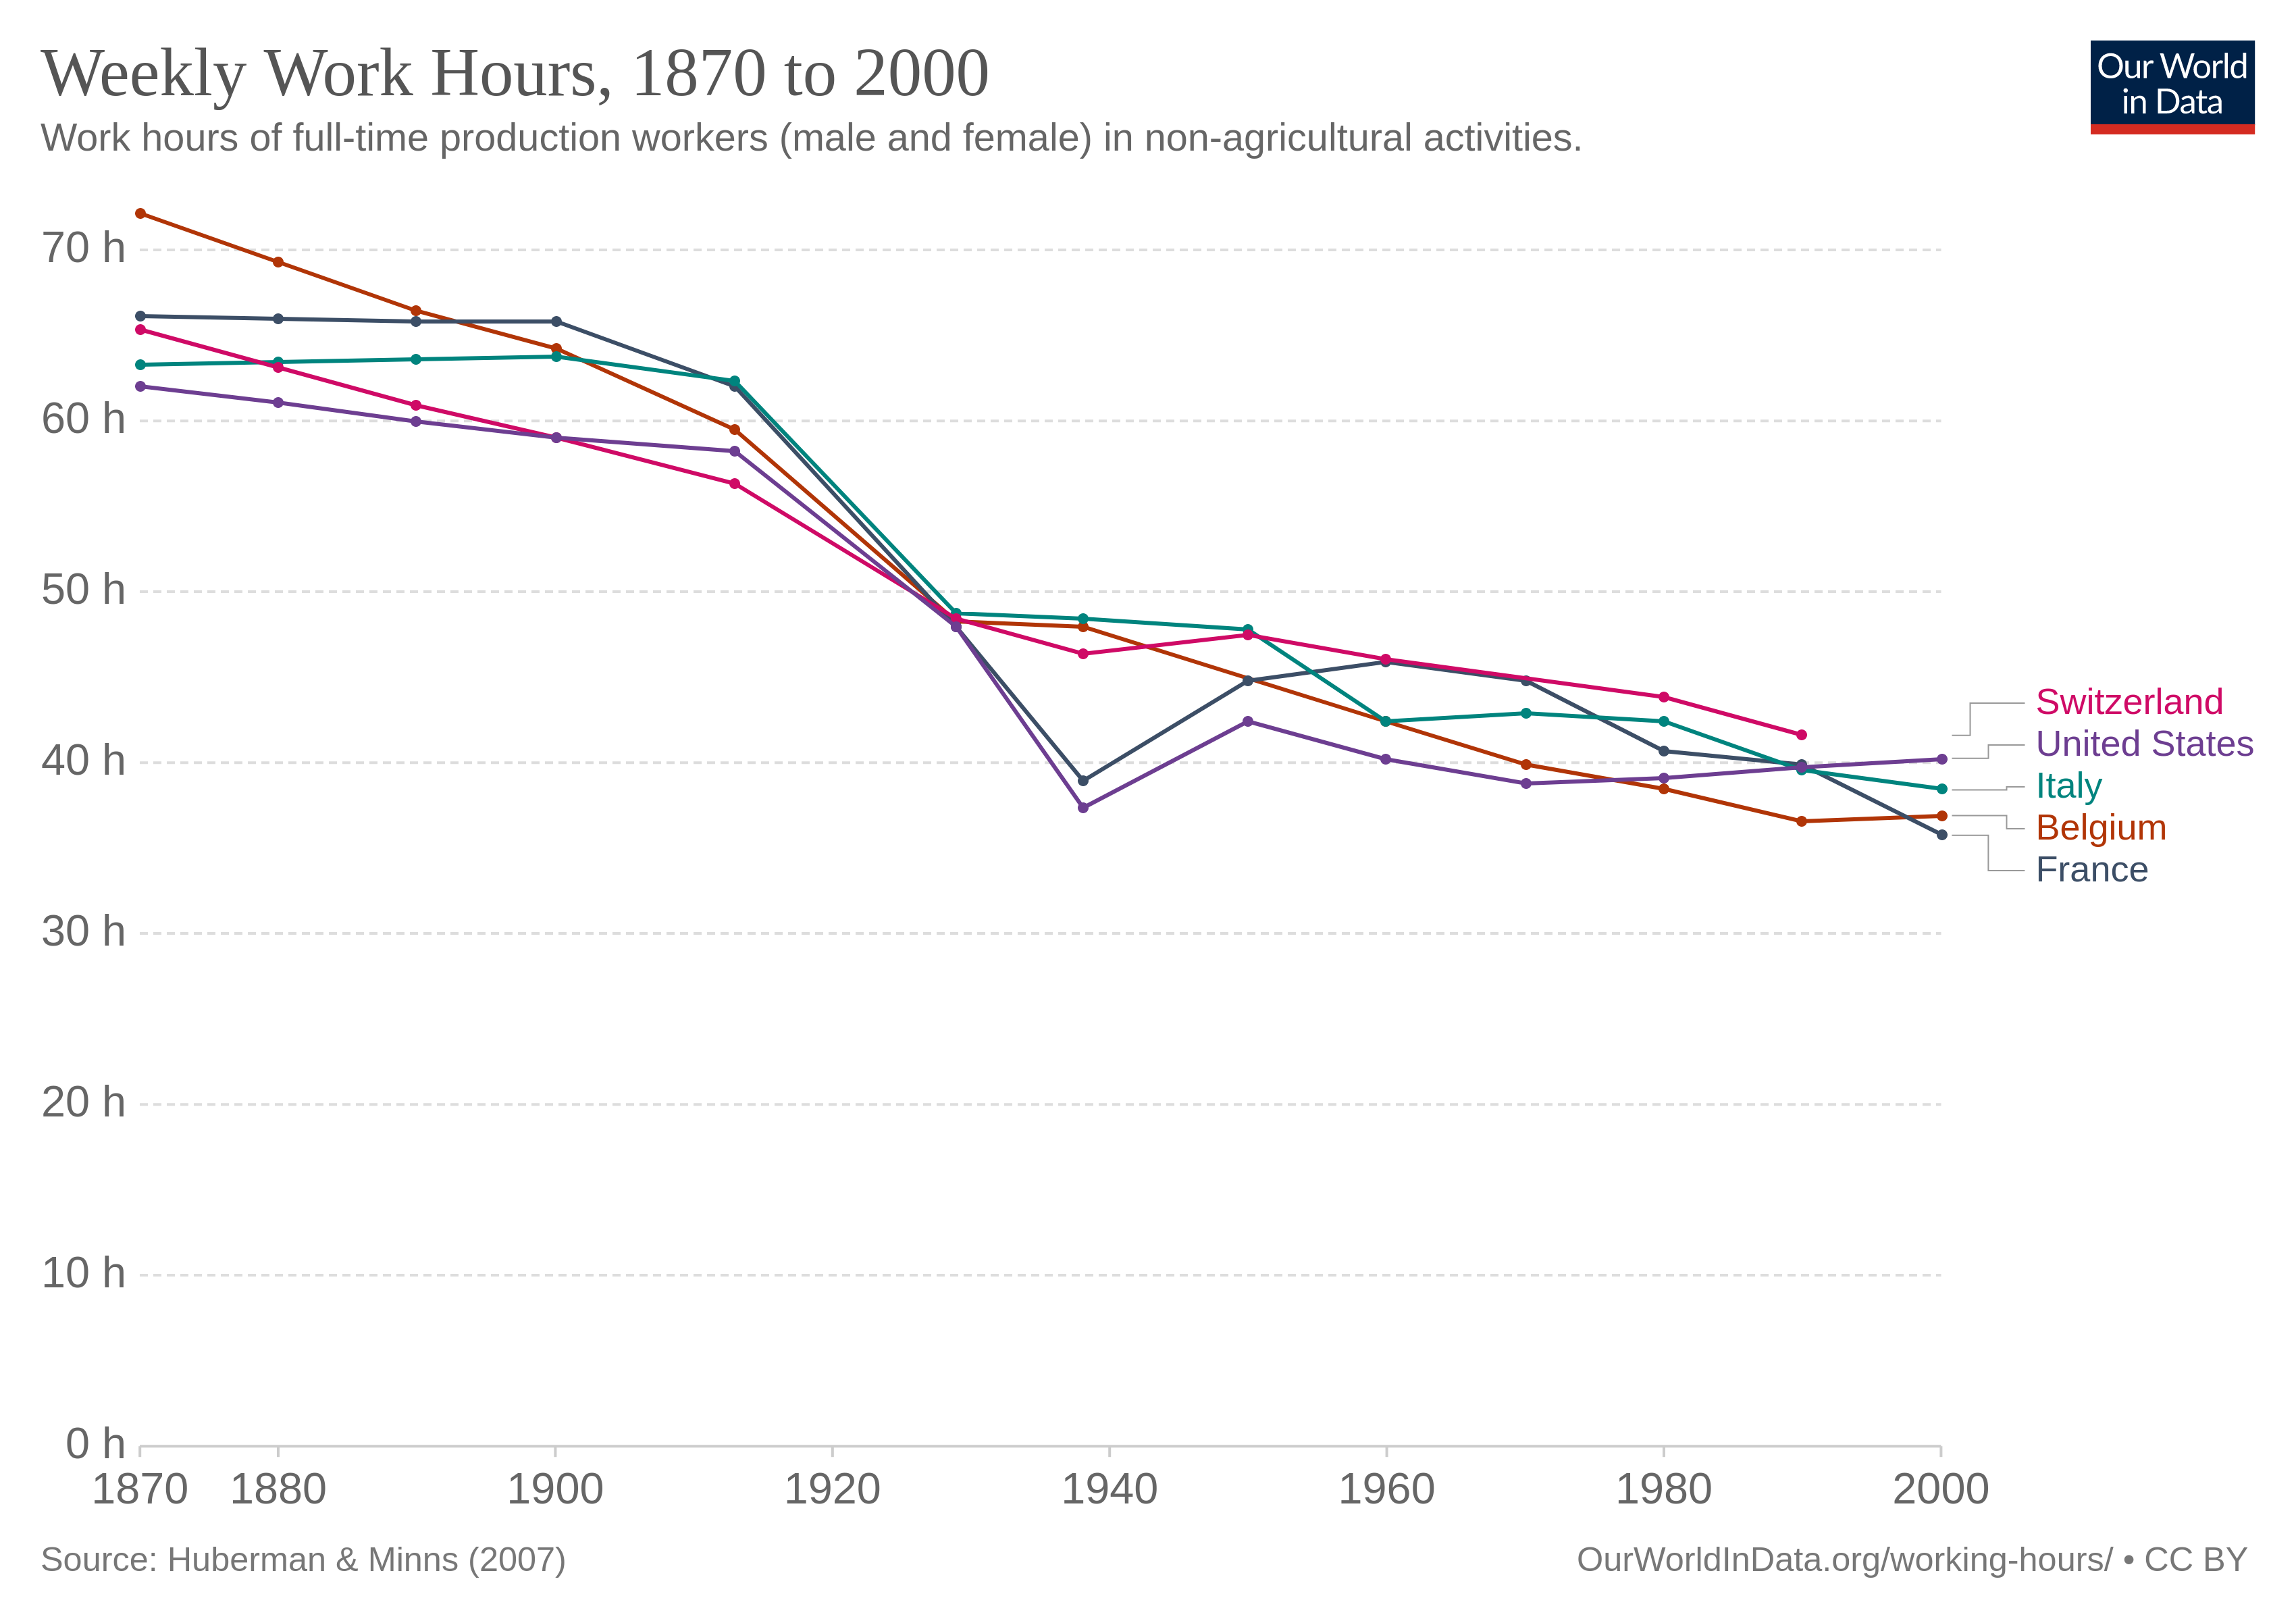
\includegraphics[width=0.8\linewidth]{images/Libro-img011.png}
    \caption{La settimana media di lavoro nel 1900 era di 60 ora mentre adesso è di 40 e, con condizioni e diritti nettamente
superiori grazie alle proteste e scioperi anche violenti scoppiati tra l'800 e il 900 e in seguito
negli anni 60 e 70
Credits: \ \protect\url{https://ourworldindata.org/grapher/work-hours-per-week?time=1870..2000\&country=BEL+FRA+ITA+CHE+USA}}
  \end{subfigure}
\end{tabular}
\end{table}

\begin{table}[H]
\centering
\begin{tabular}{cc}
  \begin{subfigure}{0.5\textwidth}
    \centering
    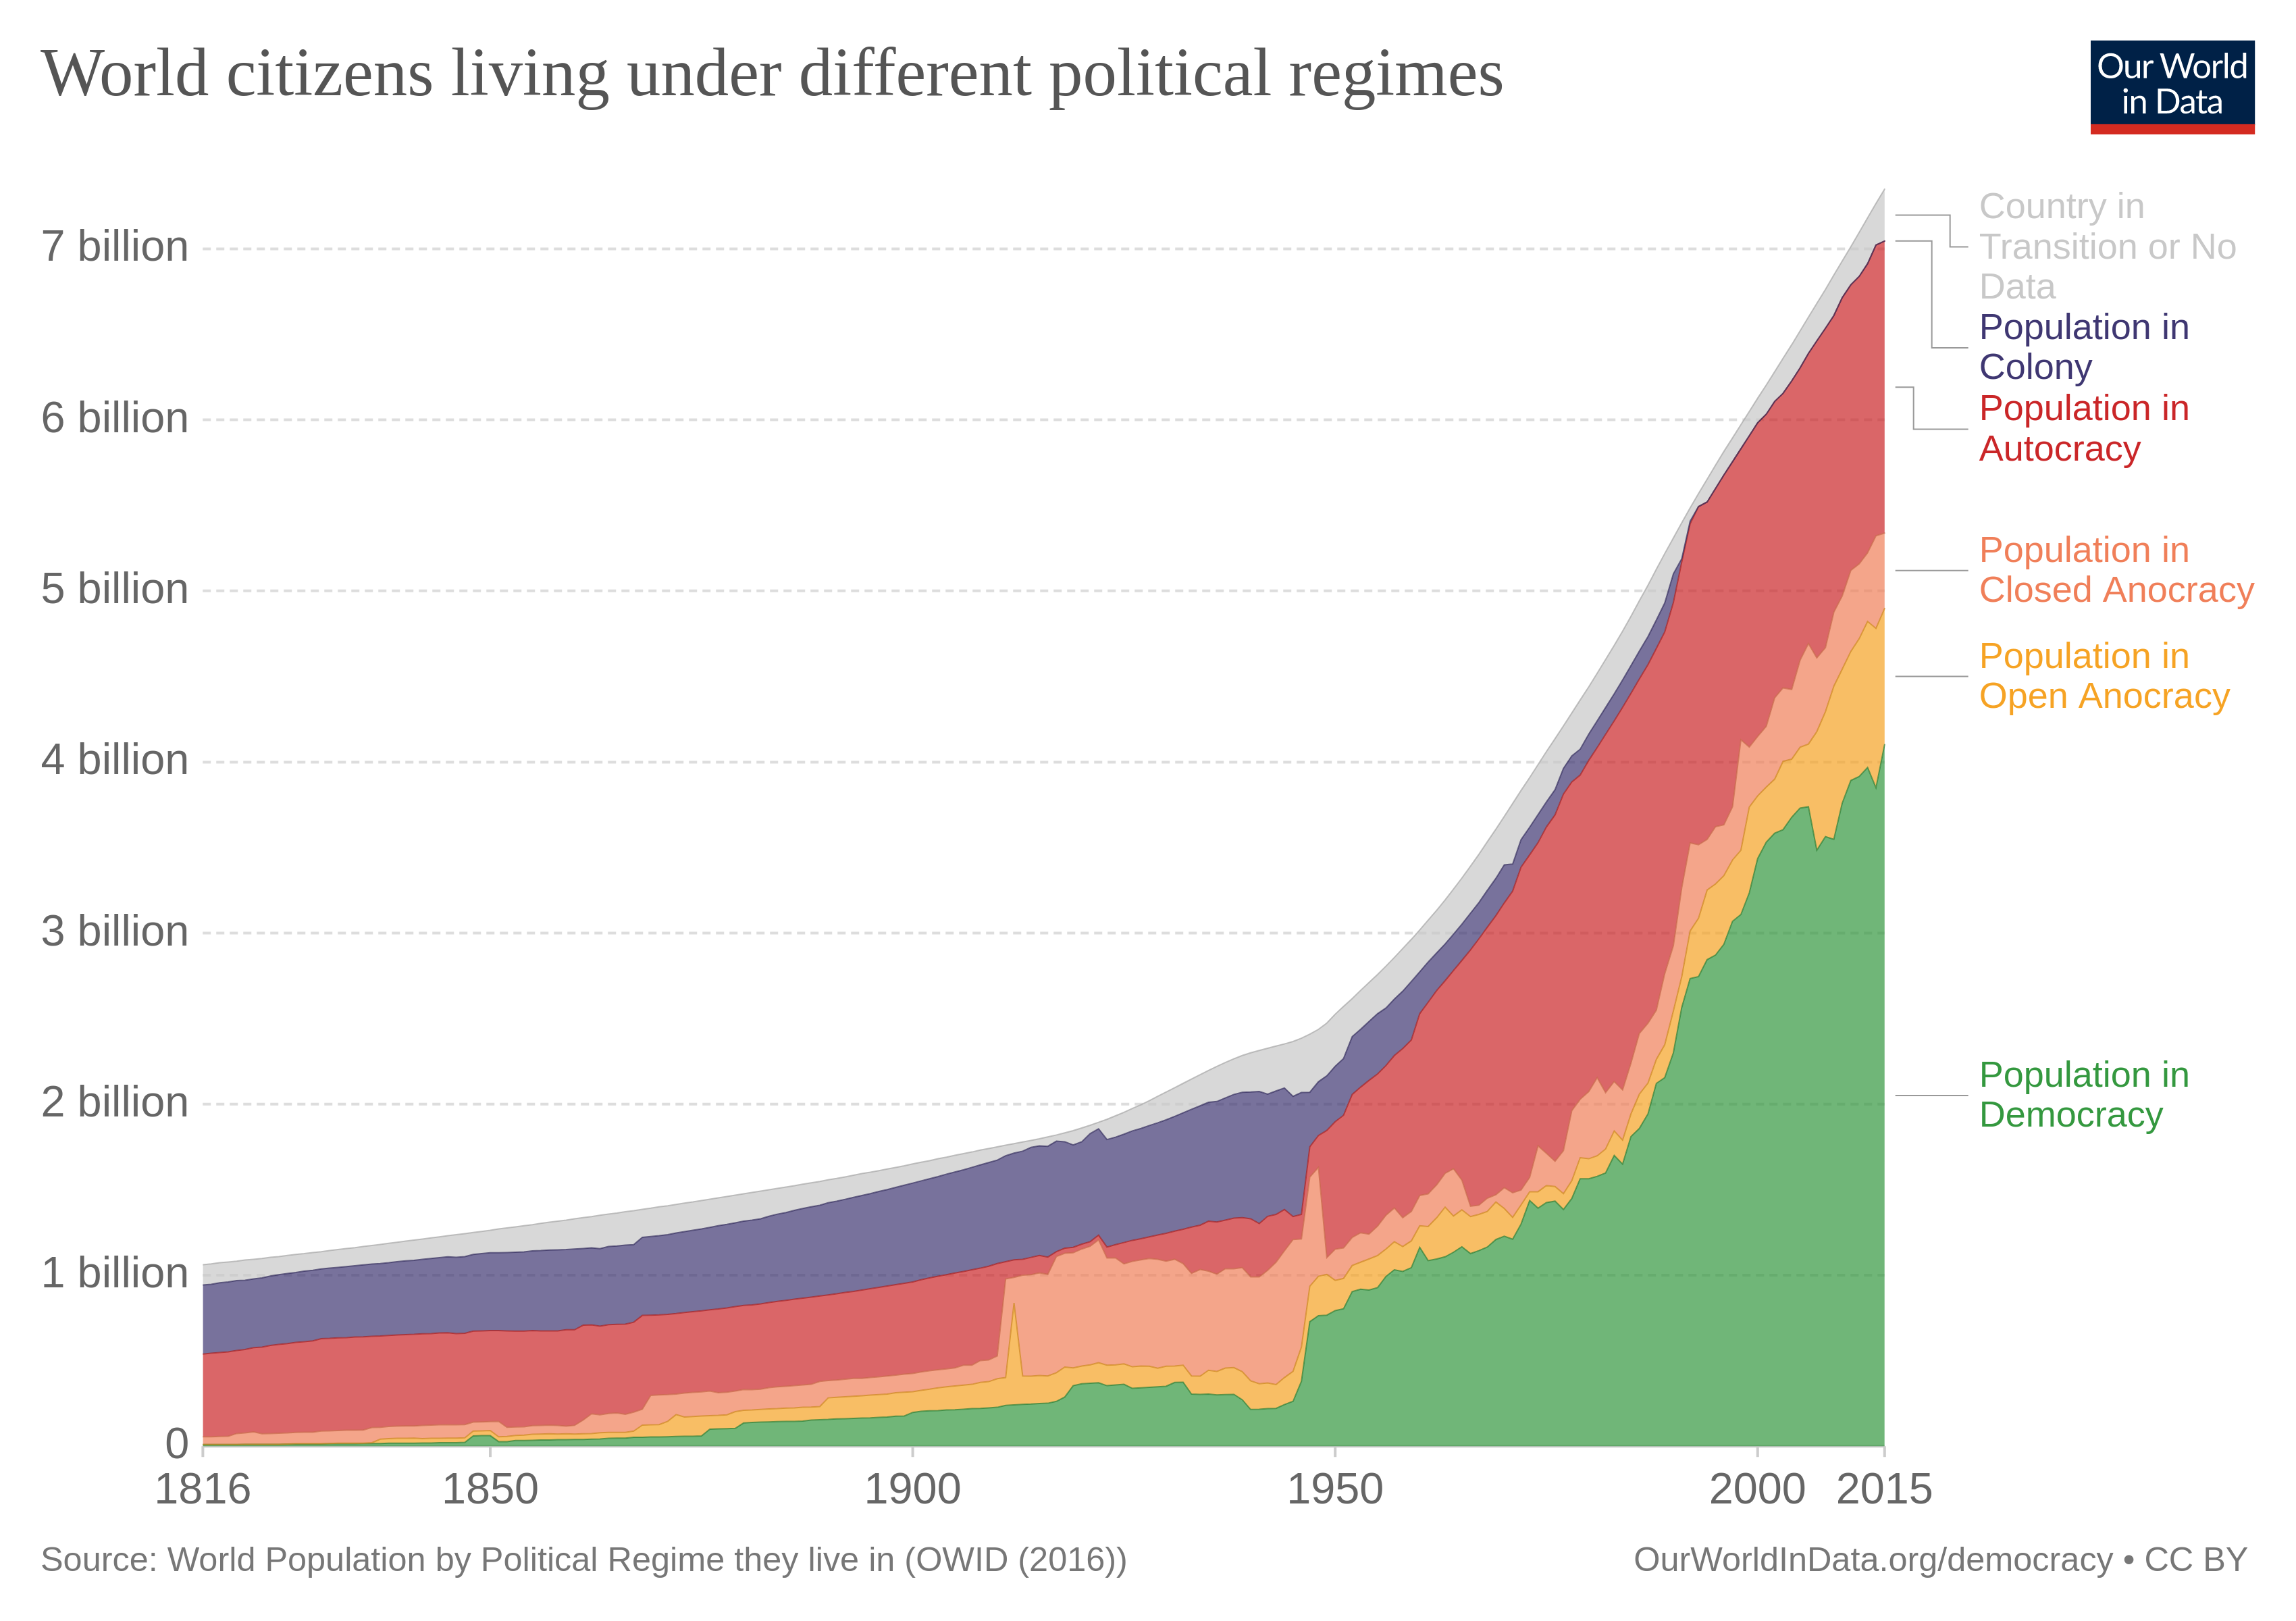
\includegraphics[width=0.8\linewidth]{images/Libro-img012.png}
    \caption{Sempre più persone vivono in governi democratici
Credits: \ \protect\url{https://ourworldindata.org/grapher/world-pop-by-political-regime}}
  \end{subfigure}
  &
  \begin{subfigure}{0.5\textwidth}
    \centering
    \caption{}
  \end{subfigure}
  \\
\end{tabular}
\end{table}

\bigskip

I morti nelle guerre diminuiscono, il terrorismo diminuisce, aumentano i diritti umani, articoli scientifici, musica,
film, \ letteratura, democrazia, anche se sembra incredibile! Potete trovare numerosi altri indici su
ourworldindata.org. E altri grafici interessanti su:

www.gapminder.org/tools

www.gapminder.org/data


\bigskip

Con questo non voglio dire che non ci siano problemi, ma dobbiamo stare attenti a non fare diventare generali, assoluti
e totali i singoli problemi. Certo, c'è ancora tanto da fare, ma la cosa importante è che la
tendenza sia positiva. Probabilmente nel 2020 avremmo dovuto aver già conquistato certi traguardi, può darsi, stiamo
andando un po' più lenti del previsto? È vero, ma la direzione, ci dicono i dati, sembra essere quella giusta in tanti
aspetti.


\bigskip
\begin{mdframed}[linewidth=1pt]
Fake news e complotti

Anche le cose più semplici, andando a un livello di dettaglio maggiore, sono molto complicate da spiegare o
contro-intuitive, ovvero fenomeni che la logica anche ragionevole spiegherebbe in un modo ma per la realtà dimostra
essere sbagliato. A scuola abbiamo visto un sacco di esperimenti di questo tipo, uno dei più famosi è la caduta dei
gravi di Galileo. Se facciamo cadere due oggetti, atterrerà per primo quello con una massa più grande. Questo ci può
portare a pensare che la velocità di accelerazione dipenda dalla massa. Se facciamo però cadere questi oggetti
all'interno di un cilindro senz'aria vedremo che gli oggetti cadono assieme.
Un altro esempio? Dimostrare che il sole esiste per come lo conosciamo, quindi come una stella dove attorno ruotano i
pianeti tra cui il nostro. Si potrebbe obiettare che invece sia una lampada gigante messa dagli alieni per farci
crescere più velocemente e poi nutrirsi della nostra energia. Senza le basi di osservazione dello spazio è impossibile
smentire il complotto. L'unico modo pratico è quello di andare in orbita con un razzo, ma siccome non possiamo farlo
tutti dovremmo fidarci di chi ci è andato. Il complotto funziona perché ci vuole un secondo per essere formulato e non
ha bisogno di prove che lo dimostrino (non è falsificabile). Mentre anche una cosa semplice, come l'esistenza del sole,
è molto difficile da dimostrare senza le basi dell'osservazione spaziale. Quindi come posso scegliere qual è la
versione giusta? Devo credere a qualcuno che lo sa verificare con i telescopi, o credere a qualcuno che è andato sullo
spazio o, credere a qualcuno che scrive un post sui social? In tutti i casi mi devo fidare di qualcuno. Per questo,
credere per credere, conviene farlo per qualcosa dove non è un singolo a dire qualcosa, ma un gruppo di esperti che
ottengono gli stessi risultati da un esperimento (peer review). Non possiamo solo affidarci alle nostre sensazione o ai
nostri sensi. Solo con lo sguardo sarebbe impossibile dire che siamo noi a girare attorno al sole. Le fake news e il
complottismo permettono di avere risposte condivisibili senza particolari competenze tecniche e, che altrimenti non si
potrebbero avere senza colmare con lo studio di anni a volte di materie complesse. Inoltre bisogna raccogliere
documentazioni, testimonianze, analisi, per demolire una teoria del complotto, o verificare le fonti, compito gravoso
che i più non fanno. Insomma è più facile credere che studiare. Anche se alcuni complottisti non hanno difficoltà a
studiare e sono molto preparati, ma indirizzano le loro energie a validare più che a criticare le loro teorie, quello
che abbiamo descritto nella filter bubble.


\bigskip

\begin{figure}[H]
  \centering
  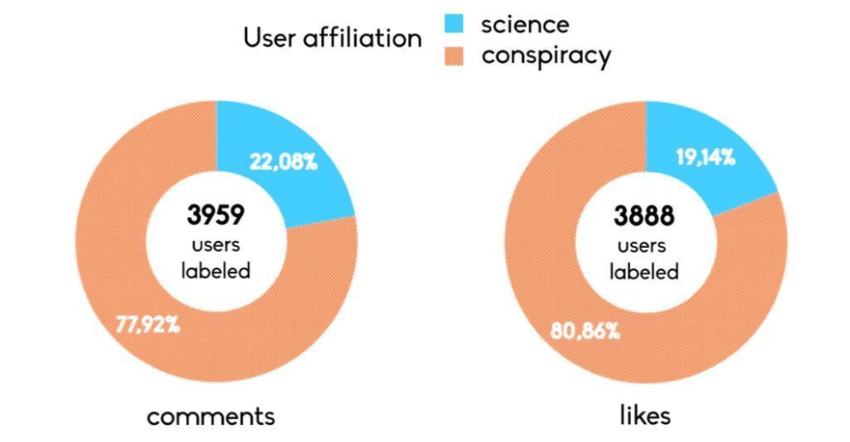
\includegraphics[width=0.95\linewidth]{images/Libro-img013.png}
  \caption{Credits: ResearchGate \protect\url{https://www.researchgate.net/figure/interaction-of-polarized-users-with-deliberately-false-information-Trolls-posts-We\_fig6\_33193629}}
\end{figure}


L'analisi riassunta da quest'immagine dimostra che i post deliberatamente
falsi, fatti per divertimento da troll o semplicemente per ricevere più click e di conseguenza più guadagni, ricevono
più like e commenti dai complottisti che, paradossalmente, nella ricerca della verità rimangono aggrovigliati in questa
rete di notizie false.


\bigskip

È giusto sottolineare che complotto non significa necessariamente falso. Non possiamo dire cosa sia vero e cosa no, ma
cosa è scientificamente provato, ovvero quelle teorie che seguono tutto il metodo scientifico. Se non è scienza è
qualcos'altro, come pseudoscienza, che magari è pure vero e un giorno la scienza riuscirà a
dimostrarlo. La questione riguarda solo il metodo che vogliamo adottare per indagare la realtà, alla luce di quanto la
nostra mente possa produrre distorsioni e fin ora il metodo più solido che l'umanità abbia
prodotto è proprio il metodo scientifico, per le ragioni viste precedentemente.


\bigskip

Quindi una domanda potrebbe essere: perché i complottisti non pubblicano su riviste scientifiche? Se hanno così a cuore
la divulgazione delle proprie scoperte? Come abbiamo visto prima, per via dell'anonimato sulle
revisioni, la scusa della censura da parte dei poteri forti non regge più. Spesso queste teorie sono fine a se stesse
non proponendo una soluzione, in questo modo queste informazioni solo solo speculazione. Proprio per questo ho sempre
trovato più interessante le motivazioni psicologiche che muovono i complottisti, più che i complotti in se. Qual è il
bisogno che ci sta dietro, che ci porta a fare ciò che facciamo? Domanda che cerco di porre a me stesso e
successivamente trasporto sugli altri.


\bigskip

Nel caso specifico dei complotti ho trovato interessante questi libri e queste ricerce:

Belief in Conspiracy Theories\endnote{\protect\url{https://www.jstor.org/stable/3791630?seq=1} \ } \ di Ted Goertzel

Misinformation\endnote{\protect\url{https://www.amazon.it/Misinformation-Guida-societ\%C3\%A0-dellinformazione-credulit\%C3\%A0-ebook/dp/B01M4NP408}
} di Walter Quattrociocchi e Antonella Vicini

Do you have to be mad to believe in conspiracy theories? Furnham \& Grover
(2021)\endnote{\protect\url{https://journals.sagepub.com/doi/10.1177/00207640211031614} }

A Systematic Review and Meta-Analysis of Psychological Research on Conspiracy Beliefs. Goreis \& Voracek
(2019)\endnote{\protect\url{https://www.ncbi.nlm.nih.gov/pmc/articles/PMC6396711/} } 


\bigskip

Probabilità del complotto

David Grimes ha proposto un metodo statistico per studiare i
complotti\endnote{\protect\url{http://journals.plos.org/plosone/article?id=10.1371/journal.pone.0147905} }. Grimes fonda la sua
teoria su una semplice idea e di buon senso: meno persone sono a conoscenza del complotto, più tempo rimarrà segreto.
Analizzando i dati del passato relativi ai complotti che sono stati scoperti è riuscito a creare un modello matematico
in grado di stimare per quanto tempo un informazione può rimanere segreta in relazione al numero di persone coinvolte,
quindi calcolare la probabilità che ci sia una talpa o la possibilità di fughe di notizie.

Un complotto può restare segreto per 5 anni se ci sono meno di 2521 persone a conoscenza e, 100 anni se i cospiratori
sono meno di 125.

Questa scoperta rende improbabili molte teorie del complotto tra cui il mancato sbarco sulla Luna scoperto in 3 anni e 8
mesi, la cospirazione sui vaccini trovata in 3 anni e 2 mesi e l'esistenza di una cura segreta per
il cancro, 3 anni e 3 mesi\endnote{\protect\url{https://www.wired.it/scienza/2016/01/29/matematica-teorie-complotto/} }.

Nemmeno le aziende farmaceutiche (Bad Pharma di Ben
Goldacre\endnote{\protect\url{https://www.amazon.co.uk/Bad-Pharma-companies-mislead-patients/dp/0007350740} }) o
l'NSA (National Security Agency) è riuscita ad eludere questa regola, famoso il caso di Edward
Snowden che denunciò lo stato americano di spiare i cittadini tramite siti come wikileaks.org o arxiv.org dove
possibile pubblicare teorie, dati alla mano.


\bigskip

Paranormale

James Randi nel 1996 Randi fondò la James Randi Educational Foundation\endnote{\protect\url{https://web.randi.org} } che studia le
affermazioni riguardanti il paranormale. La fondazione mette in palio un premio di un milione di dollari per chiunque
possa dimostrare una capacità paranormale in un ambiente controllato, quindi un video, siccome potrebbe essere stato
modificato non rappresenta una prova valida. Nessuno però è mai riuscito a superare il test preliminare, che viene
stabilito e concordato tra Randi e il candidato. Ad oggi nessuno è mai riuscito a dimostrare un fenomeno paranormale.
\ Anche il CICAP opera nello stesso campo e ha stilato una serie di
requisiti\endnote{\protect\url{https://www.cicap.org/n/articolo.php?id=273076} } alla ricerca di verificare fenomeni paranormali.
\end{mdframed}

\bigskip


\bigskip

\clearpage\section{Felicità}
\begin{mdframed}[linewidth=1pt]
Nota: Premetto che non sono uno psicologo e questo, quindi quello che segue deve essere preso in
quest'ottica. Io ho cercato di essere preciso con le note e i riferimenti ma ogni caso è a se, ad
esempio, se dovessimo trovarci davanti a una persona in crisi, potremmo essere portati a dare un consiglio ragionevole
come: fai dei bei respiri profondi e pensa a qualcosa di bello. Per alcune persone ansiose, questi consigli potrebbero
farli stare ancora peggio o provocare una fame d'aria che li farà sentire ancora più ansiosi.
Oltretutto, il dare consigli, rafforzerebbe nell'altra persona un sentimento di incapacità. O
ancora, se non si conosce il trauma e si va a scavare, il rischio è quello di far rivivere alcune esperienze e recare
un danno. Da non psicologo, preferisco ascoltare e non dare consigli non richiesti.
\end{mdframed}

Il popolare corso di Yale sulla felicità intitolato “The Science of
Well-Being”\endnote{\protect\url{https://www.coursera.org/learn/the-science-of-well-being} } spiega già dai primi minuti, grazie
alla dottoressa Laurie Santos che avere un buon lavoro, guadagnare tanti soldi, trovare il compagno della vita, avere
un bel corpo, fama e status, non vi renderà felici. La felicità non è mai causa di qualcosa. La felicità non è la
realizzazione di un desiderio, nemmeno dell'approvazione, della stima degli altri, del successo o
della popolarità.

La felicità dipende al 50 percento da fattori genetici\endnote{{}- Lyubomirsky, S. (2007). The How of Happiness: A New
Approach to Getting the Life You Want. Penguin books\newline
{}- Goldsmith, H. H. (1983). Genetic influences on personality from infancy to adulthood. Child Development, 54(2),
331–355. \protect\url{https://doi.org/10.2307/1129695\newline}
{}- Nichols, R. C. (1978). Twin studies of ability, personality, and interests. Homo, 29, 158-173.}, al 10 dalle
circostanze della vita e al 40 da azioni, abitudini, intenzioni. La percezione che abbiamo è invece molto diversa,
probabilmente attribuiamo un 90\% ai fattori esterni. Tutto passa! Anche la perdita di una persona amata in realtà è
una tristezza passeggera. L'essere umano infatti ha una forte resilienza innata, ma spesso ci
sforziamo di trattenere le emozioni, stati d'animo e pensieri auto sabotando e impedendo un
normale ritorno del benessere. Quindi è solo su questo 40\% che possiamo intervenire e fare qualcosa. Se vogliamo
essere felici non possiamo sperare di avere il massimo fattore genetico e ambientale dalla nostra e, non sarebbe ancora
comunque sufficiente, ci dobbiamo
impegnare!\endnote{\protect\url{https://www.vice.com/it/article/akzgwk/corso-di-yale-felicita-laurie-santos} } In realtà, alcuni
studi\endnote{{}- Agnoletti, M. (2022). L'Epigenetica ed il Microbiota dimostrano quanto il
contributo genetico della Felicità sia stato finora largamente sovrastimato.
\protect\url{https://www.medicalive.it/il-contributo-genetico-della-felicita-agnoletti/} \newline
{}- Agnoletti, M. (2020). L'epigenetica e la sovrastima della componente genetica negli studi
gemellari \protect\url{https://www.medicalive.it/epigenetica-e-sovrastima-della-componente-genetica-negli-studi-gemellari/} \newline
{}- Agnoletti, M. (2021). La stima della componente genetica alla luce dell'Epigenetica e della
microbiota revolution
\protect\url{https://www.medicalive.it/la-stima-della-componente-genetica-alla-luce-dell-epigenetica-e-della-microbiota-revolution/}
\newline
{}- Wong, A. H., Gottesman, I. I., Petronis, A. (2005). Phenotypic differences in genetically identical organisms: the
epigenetic perspective. Hum. Mol. Genet.,14, 11–18
\protect\url{https://academic.oup.com/hmg/article-abstract/14/suppl\_1/R11/560905.\newline}
{}- Fraga, M. F., Ballestar, E., Paz, M. F., Ropero, S., Setien, F., Ballestar, M. L., Heine-Suner, D., Cigudosa, J. C,
Urioste, M., Benitez, J., et al. (2005). Epigenetic differences arise during the lifetime of monozygotic twins. Proc
Natl Acad Sci U S A, 102, 10604–1069 \protect\url{https://www.pnas.org/doi/abs/10.1073/pnas.0500398102.\newline}
{}- Yet, I., Tsai, P. C., Castillo-Fernandez, J. E., Carnero-Montoro, E., Bell, J. T. (2016). Genetic and environmental
impacts on DNA methylation levels in twins. Epigenomics, 8, 105–117
\protect\url{https://www.futuremedicine.com/doi/abs/10.2217/epi.15.90} .}, hanno messo in luce errori metodologi circa queste
ricerche in cui hanno trovato un valore del 50\% come fattore genetici della felicità. Sembra infatti che questo valore
sia sovrastimato, così che il potere che abbiamo sulla nostra felicità sia ancora più alto.

Possiamo misurare i nostri progressi grazie al test PERMA (acronimo di Positive emotions, Engagement, Relationships,
Meaning, Accomplishment) che potete trovare su permahsurvey.com 


\bigskip
\begin{mdframed}[linewidth=1pt]
Grazie a studi reali pubblicati da giornali davvero accademici, ora sappiamo che la felicità si può raggiungere
sorridendo di più\endnote{\protect\url{https://www.eurekalert.org/pub\_releases/2011-02/msu-sfa022211.php} }, mangiando più
verdure\endnote{\protect\url{http://journals.plos.org/plosone/article?id=10.1371/journal.pone.0171206} }, non comportandosi
male\endnote{\protect\url{http://journals.plos.org/plosone/article?id=10.1371/journal.pone.0051380} }. O con otto abbracci al
giorno\endnote{\protect\url{http://www.ted.com/talks/paul\_zak\_trust\_morality\_and\_oxytocin} }. Inoltre servono, sette ore di
sonno e, mezz'ora di esercizio fisico al giorno per minimo tre volte la settimana, meglio se
all'aria aperta in quanto si tende a fare più pensieri positivi rispetto allo stare al
chiuso\endnote{Schertz, Kathryn E., et al. {\textquotedbl}Environmental influences on affect and cognition: A study of
natural and commercial semi-public spaces.{\textquotedbl} Journal of Environmental Psychology 83 (2022): 101852.
\protect\url{https://www.sciencedirect.com/science/article/abs/pii/S0272494422000974} }. E come regola generale, comunque per essere
felici bisogna variare il più possibile, anche nelle piccole cose.


\bigskip

Spendere o risparmiare? I soldi fanno davvero la felicità? Uno studio della Princeton University, condotto dal Premio
Nobel per l'economia Daniel Kahneman dice che sì, i soldi danno la felicità, ma solo fino a un tetto di 60 mila euro
all'anno, oltre quella cifra, aumentano stress e tristezza. Uno studio canadese ha stabilito che spendere per gli altri
garantisce una maggiore felicità che spendere la stessa cifra per sé. Anche, dilazionare i momenti in cui si spende
accresce la nostra felicità. Ma soprattutto i soldi danno la felicità quando ci danno più tempo, quindi è meglio pagare
un giardiniere o una domestica che comprarsi delle nuove scarpe. Anche il tempo da trascorrere da soli non va
trascurato, alcuni studi dimostrano come per essere felici necessitiamo dalle 2 alle 5 ore di solitudine vera, infatti
il tempo trascorso in famiglia non concorre ad aumentare questo conteggio. Con meno di 2 ore difficilmente raggiungiamo
il benessere ma con più di 5 ore non ci sono aumenti\endnote{\protect\url{https://youtu.be/9j5m3EoFoe8} }
\endnote{\protect\url{https://www.huffpost.com/entry/free-time-happier\_l\_61422730e4b0ab42329f3d4e}
}\ \endnote{\protect\url{https://www.cnbc.com/2022/09/08/too-much-free-time-wont-make-you-happier-says-psychologist-how-many-hours-you-really-need-in-a-day.html}
}\ \endnote{\protect\url{https://www.psychologytoday.com/us/blog/psychology-money-and-happiness/202303/research-shows-how-much-free-time-you-need-to-be-happy}
}.


\bigskip

Altri studi mettono in relazione il tempo trascorso all'aria aperta con un maggiore benessere psico-fisico. Chi vive in
città è più incline a sviluppare disturbi d'ansia e dell'umore, ma ha un cervello che tollera meglio lo stress. Può
essere più soggetto a malattie polmonari, ma ha a disposizione maggiori stimoli cognitivi, e più situazioni per
appagare la propria vita sociale (Chi socializza tutti i giorni rischia molti meno di morire rispetto a chi lo fa una
volta a settimana\endnote{\protect\url{https://www.focus.it/scienza/salute/vuoi-vivere-a-lungo-socializza-meglio-se-tutti-i-giorni}}).
Crescere vicino al mare calma, si tratta del cosiddetto "potere del blu". Una ricerca inglese condotta su 15.000 persone in 14 diversi Stati europei ha dimostrato che coloro che hanno trascorso parte della loro infanzia o hanno vissuto lungo le coste marine o grandi laghi ottengono punteggi di benessere più alti da adulti. Questa ricerca ha utilizzato i dati provenienti dalla Blue Health International Survey\endnote{International survey - BlueHealth\protect\url{https://bluehealth2020.eu/projects/bluehealth-survey/}}, un sondaggio coordinato dal Centro europeo per l'ambiente e la salute umana dell'Università di Exeter nel Regno Unito\endnote{BlueHealth - University of Exeter\protect\url{https://bmjopen.bmj.com/content/7/6/e016188.abstract}}.

Nel sondaggio, agli intervistati è stato chiesto di ricordare le loro esperienze con gli "spazi blu" vissute fino a 16 anni, nonché quanto spesso visitassero tali ambienti e quanto si sentissero a loro agio in essi. La ricerca, pubblicata sul Journal of Environmental Psychology, ha dimostrato che coloro che ricordavano più "esperienze blu" durante l'infanzia e l'adolescenza tendevano anche ad attribuire un maggiore valore agli ambienti naturali in generale e a visitarli più spesso da adulti, ottenendo così un maggiore benessere mentale.

\bigskip

In un importante studio del 2018 pubblicato su The Lancet (Chekroud et al.,
2018)\endnote{\protect\url{https://www.sciencedirect.com/science/article/abs/pii/S221503661830227X} }, è stato chiesto a 1,2 milioni
di soggetti di compilare un questionario che mettesse in relazione attività fisica, reddito e disagio psicologico, come
ansia, stress o umore basso. I risultati hanno dimostrato che le persone fisicamente attive riportavano mediamente 1,49
giorni emotivamente negativi in meno ogni mese, quindi, 18 giorni di disagio in meno all'anno,
rispetto alle persone inattive ma più ricche. Quindi, più ci si allena e più si sta bene? No, troviamo anche in questo
fenomeno un andamento gaussiano, quindi se ci si allena troppo o troppo poso il benessere diminuisce. Il picco di
questa curva, ideale per il benessere mentale, è rappresentato da 3/5 giorni di allenamento a settimana di circa 45
minuti, chi arrivava ad allenarsi fino a tre ore ogni giorno, dimostrava un benessere psicologico peggiore anche di chi
era totalmente inattivo. Inoltre, i benefici maggiori si ritrovano in sport di gruppo.


\bigskip

Un'indagine del Regno Unito condotta da Carrington nel 2016 dimostrò che tre quarti dei bambini
trascorrevano all'aperto meno tempo dei detenuti nelle carceri, mentre per il 20\% dei bambini era
normale non uscire neppure una volta in un'intera giornata! Credo che anche per gli adulti non si
otterrebbero risultati troppo diversi.


\bigskip

L'uomo è pienamente tale solo quando gioca - Friedrich Schiller 


\bigskip

Spendiamo anche due parole sulla relazione felicità e social network. Uno studio dell'Università del Michigan sostiene
che l'uso attivo dei social possa fare bene anche se può indurre a comportamenti narcisisti. Usare
i social in maniera attiva vuol dire postare contenuti mentre l'uso passivo è fruire dei contenuti
degli altri\endnote{Passive social network usage and life satisfaction among Vietnamese university students: a moderated mediation model of self-esteem and gender\protect\url{https://www.semanticscholar.org/paper/Passive-social-network-usage-and-life-satisfaction-Nguyen-Dang/7151b8ecc33af2a0b81e2244420be2f48937db75}}. Ovviamente quando qualcuno posta una foto della propria vita non sarà mentre è in coda alle poste o quando
fa la spesa, ma in vacanza o se sta facendo qualcosa di sensazionale, e la distorsione della realtà che si può avere è
che la vita si stia svolgendo ora per tutti e che tu sia l'unica persona che sta lì davanti al pc
a non fare nulla, ma non è così. Nell'altro senso, le para-relazioni dei social network appagano il nostro cervello illudendolo di avere molte relazioni, così da non farlo impegnare nella ricerca e nel mantenimento di relazioni offline più impegnative.

Un altro caso per me emblematico è stato quello dello youtuber Wesa che ha rimosso la possibilità di commentare i suoi
video, ma lasciando il suo indirizzo email per comunicare con lui. Il risultato fu che pochissimi gli continuarono a
scrivere. Probabilmente perché la mail non viene vista da tutti, non è social, manca del protagonismo e del farsi
belli.

Quindi i social sono il male? No, come spesso accade la risposta è: dipende. Uno studio\endnote{The Impact of Using Mobile Social Network Applications on Students' Social-Life \protect\url{https://www.semanticscholar.org/paper/The-Impact-of-Using-Mobile-Social-Network-on-Abdelraheem-Ahmed/0868edadf30ebb8cac8a812a3deb27d3e8f65bde}} ha riscontrato come l'uso moderato di applicazioni di social network possa migliorare le relazioni sociali, le relazioni familiari e la consapevolezza delle questioni attuali degli studenti. Mentre un uso eccessivo dei social network può avere un impatto negativo sul benessere psicologico e sulle relazioni nella vita reale. In accordo con altri studio\endnote{Comparing the Happiness Effects of Real and On-Line Friends \protect\url{https://journals.plos.org/plosone/article?id=10.1371/journal.pone.0072754}}\endnote{3 Reasons Real-Life Social Support Is Best for Mental Health \protect\url{https://www.psychologytoday.com/us/blog/the-athletes-way/202105/3-reasons-real-life-social-support-is-best-mental-health}} il numero di amici reali è positivamente correlato con il benessere soggettivo, mentre la dimensione delle reti online non è significativamente correlata con il benessere soggettivo.

\begin{wrapfigure}{i}{9cm}
  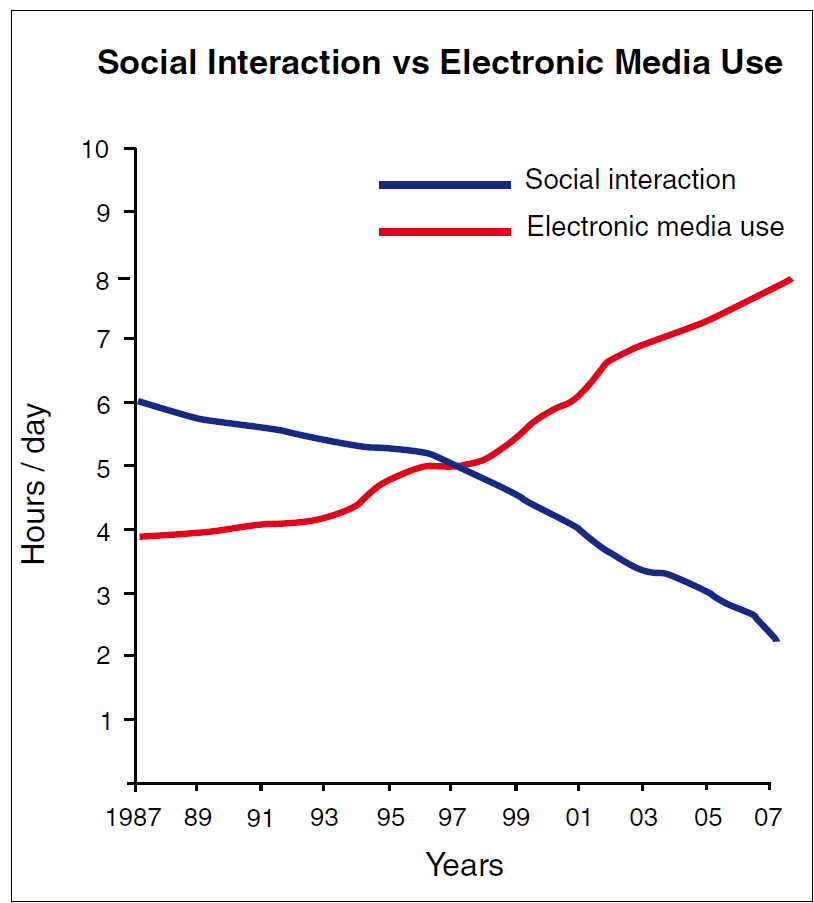
\includegraphics[width=0.95\linewidth]{images/Libro-img056.png}
\end{wrapfigure}

Un questo grafico\endnote{Well connected? The biological implications of ‘social networking’ \protect\url{https://www.aricsigman.com/IMAGES/Sigman_lo.pdf}} si vece che i media elettronici, come tv, radio, social media, rappresentati dalla linea blu, negli anni stanno occupando sempre meno tempo nella vita delle persone rispetto alle interazioni faccia a faccia. Nel 1997 il tempo trascorso con le persone reali e con le persone tramite dispositivi digitali si equivaleva e da quella data c'è stato un cambio dove le interazioni faccia a faccia sono sempre state meno rispetto a quelle digitali.

\end{mdframed}

Dagli anni 70 Nazioni Unite e Organizzazione per la cooperazione e lo sviluppo economico creano un rapporto sulla
felicità su worldhappiness.report ma uno studio pubblicato su Nature Human
Behaviour\endnote{\protect\url{https://www.nature.com/articles/s41562-019-0750-z}} ha sviluppato un modello per generare dati
precedenti agli anni 70 di Stati Uniti, Regno Unito, Germania e Italia, ma come? Analizzando libri e giornali raccolti
in Google Books, dal dal 1820 al 2009, un software tenendo conto dell'evoluzione del linguaggio ha
potuto analizzare l'umore percepito dell'epoca, quello che è emerso è che la
nostra resilienza del benessere soggettivo aumenta e diminuisce a seconda di cosa si sta vivendo, ma solo
temporaneamente. Una guerra abbassa il livello di benessere ma poi si tende a tornare velocemente al livello di
felicità percepito prima di questi eventi. Questo fenomeno si chiama habituation, funziona i grandi gruppi come uno
stato come per il singolo, succede quando perdiamo un partner, o un arto, si vive un periodo molto difficile e buio, ma
dopo due o tre anni si torna al livello di felicità percepito prima di questi avvenimenti. Stesso discorso vale anche
al contrario, l'aumento di salario ci darà felicità per un periodo, ma poi ci si
abitua\endnote{\protect\url{https://www.focus.it/comportamento/economia/felicita-nazionale-livello-secoli-passati} }.


\bigskip

“La felicità è come una farfalla; più cerchi di inseguirla, più ti eluderà. Ma se sposti la tua attenzione su altre
cose, si siederà dolcemente sulla tua spalla.” - Henry David Thoreau.

Locke:"Non sono più sperduto." 
Sun:" E come ci sei riuscito?" 
Locke:" Nel modo in cui si ritrovano le cose perdute: ho smesso di cercare...
Tratto dalla Serie TV Lost Stagione 2 episodio 5 (Oggetti smarriti)

La parola felicità, in molte lingue, come l'inglese (happiness) ha una radice che significa
“accadere”, “per caso” (happen). Mentre solitamente le persone la ricercano e poi tentano di tenerla stretta, in questo
modo perde la sua eventualità e la relativa sorpresa, novità e meraviglia. Non è soltanto una questione linguistica,
paradossalmente, se noi volessimo cercare la felicità, la prima cosa che dovremmo fare è proprio smettere di cercare.
Esattamente come sforzarsi di essere spontanei: è un errore intrinsecamente logico. Una volta che iniziamo a cercare ce
lo aspettiamo, come un pacco regalo di cui sappiamo già il contenuto, non sarà più una felice sorpresa. Forse vi sarà
capitato di aver organizzato una serata con delle vecchie amicizie, dove avere riso e vi siete divertiti più che mai.
Così, organizzate nuovamente quella serata, ma vi accorgete che l'incantesimo si è spezzato. Vi
sareste aspettati che ricreando le stesse condizioni, la gioia si sarebbe ripresentata allo stesso modo e, invece, non
è successo. 

In uno studio\endnote{\protect\url{https://psycnet.apa.org/doiLanding?doi=10.1037\%2Fa0022010} } i partecipanti sono stati divisi in
due gruppi. In uno si faceva leggere un falso articolo che illustrava i vantaggi della felicità.
L'altro gruppo, quello di controllo, invece leggeva un articolo che non faceva riferimento alla
felicità. In seguito, entrambi i gruppi hanno guardato dei videoclip che avevano per argomento la felicità o la
tristezza. I partecipanti che hanno letto l'articolo che dava valore alla felicità si sentivano
meno felici rispetto al gruppo di controllo che aveva guardato lo stesso video. Dare troppo valore alla felicità ha
aumentato le loro aspettative riguardo al modo in cui le cose “sarebbero dovute essere” e, quindi, li ha predisposti
alla delusione. Un altro
studio\endnote{\protect\url{https://www.researchgate.net/profile/Jonathan-Schooler/publication/303158395\_The\_explicit\_pursuit\_and\_assessment\_of\_happiness\_can\_be\_self-defeating\_study\_1/links/58b480a692851cf7ae941179/The-explicit-pursuit-and-assessment-of-happiness-can-be-self-defeating-study-1.pdf}
}, è giunto alla stessa conclusione. I partecipanti hanno ascoltato una canzone disarmonica: La saga della primavera di
Stravinsky. Ad un gruppo è stato chiesto di "provare a sentirsi quanto più possibile
felici" durante l'ascolto. Successivamente, sono stati valutati e
riconosciuti come meno felici rispetto al gruppo di controllo che non stava inseguendo lo uno stato
d'animo felice. 

Abbiamo molti risultati che dimostrano che sfogare la rabbia non aiuta a liberarcene o che visualizzare gli obiettivi
non aiuta il loro raggiungimento, e che nei report dei paesi più felici i manuali di self help non hanno più successo,
né la psicoterapia è più diffusa. Quindi forse la ricerca della felicità non aiuta a rendere più felici, anzi, forse il
contrario. L'intensità con cui cerchiamo la felicità è inversamente proporzionale alla possibilità
di raggiungerla. 


\bigskip

Chiediti se sei felice e cesserai di esserlo - John Stuart Mill.

\subsection{Come funziona la nostra mente?}
Questa è una domanda a cui nessuno sa rispondere in assoluto, ma forse, relativamente al benessere ne sappiamo già
abbastanza. Anzi, la cosa strana è come mai se ne parli così poco nonostante certe cose si conoscano da sempre! Infatti
tante cose che la scienza moderna sta scoprendo erano già state intuite attorno al 500 a.C. Uno dei nodi più cruciali è
stato ben espresso molti anni dopo:

“Ciò che turba gli uomini non sono le cose, ma le opinioni che essi hanno delle cose”. Epitteto.

Il nostro benessere è strettamente correlato ai giudizi e alle aspettative, che sono una forma di giudizio. Noi siamo
turbati quando abbiamo aspettative sul mondo, il futuro, le persone, ma anche giudizi sui nostri pensieri, in quanto
crediamo di essere i nostri pensieri.

Il compito del cervello non è quello di generare verità, su di noi o sul mondo, ma quello di fare ipotesi e contro
ipotesi. Il nostro cervello pensa a tutto e pure al suo contrario, per questo motivo non può dire chi siamo! Ma perché
è così contraddittorio? Tutto il nostro organismo è costruito per farci sopravvivere, e il cervello, attingendo dal
passato prova a creare ipotetici scenari sul presente e sul futuro in modo da farci trovare pronti anche alle
eventualità più remote e improbabili. Non dovremmo preoccuparci se la nostra mente è insicura, al contrario! Ci
dovremmo preoccupare se non avessimo mai dubbi, soprattutto dopo che abbiamo visto i vari bias cognitivi. 

Facciamo un gioco, ora ti chiederò di fare una cosa, sei pronto?

NON pensare a un elefante bianco. 

Cos'è successo? Scommetto che nella tua immaginazione è appena apparso un bellissimo elefante
bianco! Ma perché? Eppure ti è stato chiesto di non fare proprio quello, avresti potuto fare altro e pensare a
qualsiasi altra cosa ma non quello! Come dicevamo, il compito del cervello non è fare quello che gli diciamo, non è
quello di dire la verità su cosa sentiamo su di noi, gli altri o le cose in generale, non è quello di dirci cose carine
o motivarci, ma semplicemente simulare ipotesi e il loro contrario. Se crediamo di essere delle cattive persone, la
nostra mente che può generare di tutto e, anche il suo contrario, saprà trovare episodi in cui siamo stati cattivi, o
potrebbe reinterpretarli alcuni neutri, ma in una luce negativa. Se ci convincessimo che siamo sempre cattivi la nostra
mente inizierà a dirci: No, non è vero, in questi episodi sei stato bravo! Insomma, se noi cerchiamo qualche pensiero,
sicuramente lo troveremo (rebound effect) e possiamo fare anche il contrario. Per questo frasi come “dai... Cerca di
non pensarci!” non possono funzionare. L'unica cosa che possiamo fare è accorgerci di un pensiero
e ritornare su quello che stavamo facendo, ma con gentilezza, senza punirci per aver fatto quel pensiero. È un
po' come fare qualcosa mentre si ascolta la radio, se ci sforziamo di non ascoltarla, succede
proprio l'opposto. Mentre se ci concentriamo sul nostro compito senza sforzarci di non ascoltare
la radio, quest'ultima diventerà un suono di sottofondo.

Quando cerchiamo di non pensare a qualcosa, come un elefante bianco, la nostra mente periodicamente dovrà chiedersi:
come sta andando il mio tentativo di non pensare a un elefante bianco? E in quel esatto istante dovrà per forza
rievocare questa immagine. Una tecnica nota come “intenzione paradossale” aiuta in questo, in quanto intenzionalmente
portiamo attenzione al pensiero che stiamo cercando di evitare. In alternativa siccome non possiamo non pensare,
possiamo però pensare ad altro e, portare l'attenzione su ciò che stavamo facendo. 

Ma se sono troppo indulgente con me, ricadrò sempre negli stessi pensieri negativi! 

In realtà no, se siamo troppo severi con noi stessi, le probabilità che in futuro ci potremmo accorgere nuovamente di
questi pensieri diminuisce, perché il nostro cervello cerca di ammonire qualcosa che ci fa stare male. 

Ma allora il giudizio, anche quello sui nostri pensieri è sempre negativo?

No, il giudizio è fondamentale per prendere decisioni. Il problema è quando lo facciamo inconsapevolmente, senza
l'aver scelto consapevolmente di indirizzare la nostra attenzione e i nostri giudizi verso la
risoluzione di un problema. Giudicare i nostri pensieri è sempre sbagliato come abbiamo visto, per la natura stessa del
cervello. Mentre giudicare le nostre azioni invece è molto proficuo. Noi non siamo i nostri pensieri ma le nostre
azioni. Aristotele diceva che siamo quello che facciamo ripetutamente, non ciò che diciamo di essere. Anche qua però, anche se ci accorgiamo di non aver agito come avremmo voluto, non dobbiamo metterci in croce, perché altrimenti le probabilità che commetteremo nuovamente quell'errore aumenteranno. 

Ma quindi chi siamo? Il nostro corpo è un accumulo di cibo, può essere tuo ma non può essere te. I tuoi pensieri sono un
accumulo di cose che hai visto, cose che ti hanno detto, ragionamenti, quindi possono essere tuoi ma non possono essere
te. Alcuni filosofi hanno detto che noi siamo le nostre azioni, Quindi chi siamo\endnote{“Conosci te stesso” può
diventare un ossessione \protect\url{https://www.youtube.com/watch?v=V61SSJL-gLo} }? Qual è il senso della vita? Queste sono domande
potenzialmente pericolose perché non troveranno mai una risposta certa e si potrebbe finire in una spirale infinita. Ma
sono anche domande che è giusto porsi! Cerchiamo però di non tenerle troppo nella nostra testa, magari scriviamole o
parliamone con qualcuno per non rischiare di rimanere intrappolati. Quando pensi, pensi a tutto e al contrario di tutto, mentre quando scrivi, devi prendere piccole decisioni. Però scrivere domande senza risposta per lenire l'angoscia, come trovare il senso della vita, chiedersi se sia la persona giusta, chi sono io ecc... Potrebbe fare più male che bene. 
Secondo Gennaro Romagnoli la maggioranza delle persone che vanno in analisi da uno psicologo è perché si fanno domande irrisolvibili come Queste.

\bigskip

Un esercizio interessante potrebbe essere quello di
chiedersi: sono i miei vestiti? Sono i miei figli? Sono il mio corpo? Sono i miei pensieri? Sono la mia casa? Ci
accorgeremo che è impossibile trovare il nostro io. Il nostro io ci accade. A volte ci accorgiamo di aver reagito ad un
certo avvenimento in maniera inaspettata da quello che avremmo pensato, positivamente o negativamente; è capitato a
tutti. L'io è il rapporto tra la nostra genetica, la nostra storia e, il momento attuale. Possiamo
essere testimoni del nostro io e vedere come sta accadendo, come si sta manifestando. Questo ragionamento non serve a
deresponsabilizzarci e giustificare le nostre azioni come se compiute da un io che non siamo noi e non riconosciamo, ma
al contrario! Serve a non negare nessuna parte di noi, nemmeno le più inaspettate e, sapendo quindi che ci sono e
possono manifestarsi, saremo in grado di farci trovare più pronti a gestire questi lati che possono essere
disfunzionali o dannosi per gli altri e noi stessi.

Non siamo i nostri pensieri! I nostri pensieri nascono senza il nostro controllo, come abbiamo visto con
l'esercizio dell'elefante, vanno presi come ipotesi che il nostro cervello
porta alla luce, ma sta poi a noi valutare se prenderle in considerazione o scartale, sempre consapevoli che tutti noi
abbiamo bias cognitivi, e che le nostre valutazioni, anche le più attente, sono deformate e potrebbero quindi non
essere vere, non dobbiamo quindi giungere a conclusioni troppo affrettate su di noi e sul mondo. Esistono tecniche
ipnotiche per poter parlare con il proprio inconscio e fargli domande, come ad un'entità più saggia e separata da noi.
Seppur sia affascinante, il nostro inconscio è molto bravo a rispondere a domande come: siamo affamati? Mentre domande
come: dovrei stare o lasciare questa persona? Non produrrebbe le decisioni migliori per noi. 

I pensieri quindi possono essere veri (si chiamano “fatti”) o falsi, ma nella maggior parte dei casi non sono ne
l'uno ne l'altro, sono semplicemente storie circa il nostro modo di vedere il
mondo (“opinioni”, “atteggiamenti”, “giudizi”, “ideali”, “convinzioni”, “teorie”, “morale”). In diverse strategie, come
l'ACT (A = Accetta i tuoi pensieri e le tue emozioni C = Connettiti con i tuoi valori T = Traduci
i tuoi valori in azioni efficaci) non si cerca di capire se un pensiero sia vero o falso, ma se è utile o no. Se
prestiamo attenzione a questo pensiero, potrà esserci utile a costruirci la vita che vogliamo?

Quando prendiamo i pensieri come dei fatti reali, senza distinzione, si parla di “fusione”. In questo stato crediamo ai
nostri pensieri pensieri, ci sembrano realtà o degli ordini e, che stiano accadendo veramente. Quando la mente
partorisce un pensiero che ci disturba, del tipo “io sono X”, come “io non valgo abbastanza”, dovremmo accorgercene e
trasformarlo in “sto avendo il pensiero che io sono X”. I pensieri non sono ordini, siamo sempre noi a distinguerli tra
utili e inutili e, in questo secondo caso, ci accorgiamo e notiamo il pensiero ma non gli diamo retta. Non è un
problema il pensiero negativo, lo diventa quando noi ci fondiamo; è nel momento in cui ci crediamo che diventa un
problema. Come abbiamo visto, non possiamo scegliere i pensieri che ci passano per la testa e anche leggendo libri,
facendo seminari, diventando bravi ad applicare tutte le tecniche, i pensieri negativi continueranno ad esserci, solo
che non gli daremo più troppo peso. Lo scopo non è eliminare un pensiero, ma vedere i pensieri per ciò che sono: delle
ipotesi. 

Quindi la fusione o i pensieri negativi sono il problema? Quando sei assorto in un progetto, nella risoluzione di un
problema, in una conversazione, sogni ad occhi aperti, dalla lettura di un libro o dalla visione di un film, sono tutte
attività che implicano la fusione, ma migliorano anche la tua vita. La fusione diventa un problema soltanto quando ti
impedisce di vivere pienamente la tua vita. Lo stesso discorso vale per i pensieri negativi, che servono per non farci
trovare impreparati o per farci capire che quella non è la nostra strada, o che il rischio è troppo alto. 

Possiamo dividere la nostra esperienza come vissuta da due sé, quello pensante e quello osservante. Il sé pensante è la
parte di te che pensa, pianifica, giudica, confronta, crea, immagina, visualizza, analizza, ricorda, sogna a occhi
aperti e fantastica, o più in generale la “mente”. Il sé osservante invece è consapevole, ma non pensa, ed è
responsabile della concentrazione, dell'attenzione e della consapevolezza. Può osservare o
prestare attenzione ai tuoi pensieri, ma non li può produrre. Ad esempio se stai giocando a tennis e sei completamente
concentrato sulla pallina, senza pensare a nient'altro, allora sta operando il tuo sé osservante.
Se invece, mentre giochi, stai pensando: “non sto impugnando bene la racchetta”, “devo concentrarmi di più”, “il
prossimo punto è decisivo”, “ora farò un bel tiro” ecc… allora qua è il tuo sé pensante che sta operando e non ti sta
facendo giocare al meglio. Possiamo rimanere concentrati su quello che stiamo facendo e contemporaneamente sulle proprie sensazioni perché sono due sistemi leggermente separati. All'inizio è complicato ma con l'allenamento ci si può riuscire dice Gennaro Romagnoli.


\subsection{Come gestire il proprio mondo interiore?}
“Ciò che turba gli uomini non sono le cose, ma le opinioni che essi hanno delle cose” scriveva Epitteto 2000 anni fa.
Qua potrebbe concludersi questo capitolo, siccome in questa frase è racchiusa tutto ciò che serve sapere. Una frase
semplice, forse addirittura banale da comprendere ma molto difficile da applicare, perché come detto in precedenza i
nostri pensieri sorgono spontaneamente portando con se le relative opinioni e giudizi. Ma come possiamo interrompere
questo automatismo? Non possiamo smettere di pensare e non sarebbe nemmeno questo il problema. Il problema sono le
opinioni e i giudizi sui pensieri. O meglio, saper giudicare qualcosa è uno strumento importante e ogni tanto è
fondamentale valutare le nostre azioni, anche se questo non ci fa stare bene. Il problema non è il giudizio, il
problema è il giudizio inconsapevole. Il problema è quando più o meno costantemente durante la giornata siamo messi
sotto inquisizione dal nostro giudice interiore. Se lo facciamo consapevolmente, dedicando un momento durante la
giornata, magari in maniera strutturata con la scrittura espressiva che vedremo più avanti, possiamo contenere questo
giudizio ed eventuali emozioni negative in un lasso temporale, se diventa consapevole invece non
c'è un limite ne una struttura a contenerlo, ne una possibile fine che ne definirà una
conclusione. Se invece tutti i giorni definiamo un momento per ripensare a qualcosa che ci turba, ci accorgeremo che
dopo qualche giorno non sapremo più cosa dire, mentre se non diamo una struttura al nostro rimuginio, possiamo produrre
e rimasticare gli stessi contenuti all'infinito, non producendo nulla di nuovo. Stesso materiale,
stesse informazioni, stessi schemi mentali, non possono produrre nuove soluzioni. 

I problemi non possono essere risolti allo stesso livello di conoscenza che li ha creati - Albert Einstein

Quindi se stiamo lavorando, passeggiando, studiando, giocando o qualsiasi altra cosa, appena ci accorgiamo che stiamo
facendo un pensiero che non riguarda l'attività che stiamo svolgendo, riportiamo gentilmente
l'attenzione a ciò che stiamo facendo. 

Questo è tutto.

Come dicevo precedentemente è facile da capire ma non da applicare. Questa operazione contiene tre concetti chiave:
consapevolezza, giudizio, gentilezza.

Consapevolezza. Quante volte ci capita di pensare a qualcosa e rincorre per minuti o ore questo contenuto mentale
riempendolo di ulteriori parole e giudizi? E dopo qualche ora ci accorgiamo che la mente ha vagato per tutto questo
tempo mentre stavamo facendo altro? Magari litighiamo con un collega e tutto il viaggio di ritorno ci abbiamo pensato e
ad un certo punto ci troviamo a casa, come se ci fossimo teletrasportati, come se ci fosse un blocco di memoria
cancellata. A volte rischiamo così di perderci dei momenti importanti. Appena ci accorgiamo di non essere concentrati
sul presente, diventiamo consapevoli e possiamo intervenire in qualche modo, avere un margine di manovra sul nostro
mondo interiore. Se non diventiamo consapevoli, non possiamo fare nulla, e ci troviamo ancora a rincorrere quello a cui
stavamo pensando. Ma come possiamo diventare consapevoli più spesso? L'esercizio più importante
per allenare la consapevolezza è la meditazione, che vedremo tra poco.

Giudizio. Questo punto è quello più comprensibile apparentemente, ma in realtà contiene dei tranelli al suo interno. Se
ci accorgiamo che stiamo facendo un giudizio su una cosa negativa, è intuitivo che dovremmo gestirlo, ma il tranello è
la gestione anche dei giudizi su cose positive. Ad esempio, se ci accorgiamo che non eravamo concentrati su quello che
stavamo facendo, è una cosa positiva, ma potremmo trasformarla in una cosa negativa se ci giudichiamo negativamente per
non essere riusciti a rimanere concentrati (è impossibile rimanere sempre concentrati). E se dovessi sforzami di
provare emozioni positive? Sto comunque dando un giudizio a ciò che provo e potrebbe sfociare in un pensiero negativo,
perché molto spesso poi si incappa in pensieri tipo: sto provando sensazioni abbastanza positive? Dovrei provarne di
più? Eppure non mi manca niente, perché non sono euforico? Forse dovrei ottenere altro dalla vita? Portando così ad un
aspirale infinita, perché non c'è un limite, non c'è qualcosa di oggettivo che ti farà dire, sì ora è abbastanza. La
pienezza è una ricerca vana non sarai mai pieno abbastanza. Quindi è sbagliato interrogarsi sulla felicità, il vero
amore o il senso della vita? No, ma queste domande senza risposta è meglio non tenerle nella propria testa, perché sono
potenzialmente infinite e angoscianti, meglio dargli una struttura come dicevamo prima e farle uscire dalla nostro
pensiero parlandone con qualcuno o scrivendo. Solitamente mentre stiamo facendo un'attività
piacevole. L'effetto di questa domanda è il blocco immediato delle sensazioni piacevoli, perché la
nostra attenzione verrà spostata dall'esperienza che stiamo vivendo alla domanda e questo
intellettualmente non finirà mai non avando una risposta. Riflettere sul senso profondo di ogni cosa che si sta
vivendo, infatti, è una delle istruzioni per rendersi la vita infelice secondo Paul Watzlawick. Come scrive George
Leonard in Mastery: L'essenza della noia si trova nella ricerca ossessiva di novità. Probabilmente
siamo spesso felici, nel senso più realistico e che dovremo dare a questo termine, ma con le definizioni che invece
abbiamo possiamo dire che siamo sempre felici, tranne nel momento in cui ce lo chiediamo.

Gentilezza. Diventa così chiaro perché è importante questo punto. Se non lo faccio con gentilezza sto giudicandomi
negativamente. Essendo impossibile non pensare e far sorgere i giudizi che sono le opinioni sulle cose che creano
turbamento di cui parlava Epitteto, la cosa giusta da fare e ritornare a ciò che stavamo facendo senza aggiungere un
ulteriore giudizio. Se iniziamo a giudicare quando ci accorgiamo che non eravamo concentrati sul presente, il nostro
cervello, per preservare il suo benessere, ammonirà questo comportamento e di conseguenza le probabilità che
diventeremo consapevoli ancora si abbasseranno togliendoci ogni possibilità di autogestione e lasciando così i giudizi
a piede libero.

Tutti questi concetti li ho presi in prestito da Gennaro Romagnoli uno psicologo e psicoterapeuta che conduce il podcast
di Psinel e autore dei libri Facci caso e Restare in piedi tra le onde.

Ma quindi si può essere felici? Siccome giudicando la felicità non sarà mai abbastanza? Io eviterei di chiedermelo e se
sorge questa domanda ritornerei a ciò che stavo facendo, godendomi il momento e concentrandomi sulle mie sensazioni
corporee e così sarai felice, anche se non te lo sarai verbalmente detto. 

Quindi non devo sforzarmi di essere felice? Io dovrei fare ciò che reputo importante secondo i miei valori e non ciò che
è importante per le richieste sociali, anche se questo richiede fatica e, ogni volta che agisco in questa direzione, se
sento un giudizio, come al solito lo noto e ritorno gentilmente a ciò che stavo facendo. In questo modo ci sarà il
miglioramento ma contenendo la parte negativa di questo processo. 

più ti sforzi di stare continuamente bene e meno sarai soddisfatto - Alan Watts


\bigskip


\bigskip


\bigskip


\bigskip


\bigskip


\bigskip


\bigskip

\begin{mdframed}[linewidth=1pt]
Noia

In un esperimento sono state lasciate delle persone sole per quindici minuti in una stanza vuota, con solo un pulsante
rosso che dava delle scosse (sopportabili). La metà dei partecipanti, per combattere la noia, preferivano premere il
pulsante e, prendersi la scossa, piuttosto che non far nulla. Il dolore diventa quindi preferibile della noia, al non
pensare. Addirittura un partecipante ha premuto il pulsante 190 volte in quei 15
minuti.\endnote{\protect\url{https://www.bbc.com/news/science-environment-28130690}} Uno studio dell'università della Pennsylvania
ha dimostrato che più ci si annoia meno siamo soddisfatti della nostra vita. Bastano soltanto due ore di noia per
percepirlo. Allo stesso tempo però la noia può capitare e con la meditazione impariamo a gestirla e sopportarla meglio.
Se non ti piace la noia é perché forse in quel momento affiorano dei contenuti che non vuoi affrontare. Nota cosa emerge e poi in un secondo momento usa la scrittura espressiva  per elaborarlo.
A volte il tempo presente può anche sembrarci pieno e tuttavia nel ricordo vuoto. La noia viene vissuta come mancanza
di significato, dinanzi a un tempo vuoto l'animo umano prova orrore, pena e disgusto.

Secondo lo Anna Gosline\endnote{\protect\url{https://www.scientificamerican.com/article/the-science-of-boredom/}}, la noia non é né positiva, né negativa, é solo uno stato, ma se proptratto nel tempo può portare alla depressione. La noia non sembra nemmeno essere correlata alla creatività. 
I ricercatori non dicono di cercare la noia ma anche di non evitarla non con metodi di intrattenimento passivi, come TV, social network ecc...

Secondo Adam Grant, l'antidoto contro il languore, ovvero quella sensazione dove non c'è nulla che i quel periodo ti
entusiasmi, non dev'essere qualcosa di produttivo, ma di divertente, che faccia sentire concentrati e competenti con le
persone amate, come ad esempio una partita ad un videogame come Mario
kart\endnote{\protect\url{https://www.ted.com/talks/adam\_grant\_how\_to\_stop\_languishing\_and\_start\_finding\_flow?language=it}
}. Inoltre tutti i giochi, anche i videogiochi aumentano la neuro plasticità. Se giocare ti fa sentire in colpa, ma al
contempo ti piace anche farlo, semplicemente nota come ti comporti e cosa pensi. In generale, per riaccendere la curiosità bisogna provare cose nuove, accedere a nuovi stimoli. Statisticamente prima o poi troverai qualcosa che ti accende.

Anche gli animali si annoiano? Sì! Secondo lo studio del Royal Veterinary College di Londra condotto da Charlotte Burn e
pubblicato sulla rivista Animal Behaviour. I test effettuati su topi, cani, cavalli e muli hanno dimostrato che se
impegnati in attività sgradite o nessuna attività, gli animali si comportano in modo anomalo come l'iperattività, una
forte sensibilità agli stimoli esterni o con azioni ripetitive. Non è ancora chiaro come gli animali percepiscano lo
scorrere del tempo, ma i topi da laboratorio ad esempio giocano con gli interruttori della luce, continuando a
spegnerla e accenderla. 
\end{mdframed}


\bigskip

Rimuginio

Per la nostra crescita personale non dobbiamo distinguere in pensieri giusti o sbagliati, buoni o cattivi ma come utili
o inutili, produttivi o improduttivi. Dobbiamo quindi cercare la resilienza e non la resistenza. La resilienza è il
tempo che impieghi a tornare in uno stato di quiete. Mentre il prodotto tra la resistenza e il dolore/disagio che
stiamo provando provoca la sofferenza. Il dolore capita, la sofferenza la creiamo noi. Numerosi studi dimostrano come i
dubbi appaiono e scompaiono in maniera naturale, ma chi rimugina sui propri pensieri non permette questo naturale
flusso di di coscienza di scorrere normalmente. Siamo quindi noi a trattenere questi pensieri che ci fanno soffrire e
che altrimenti in maniera naturale scomparirebbero. Il rimuginio, ovvero l'attività di pensare e
ripensare in maniera ripetitiva, ha l'obiettivo di trovare soluzioni a un possibile futuro evento, ma quello che in
realtà fa è crearne di nuovi. Per esempio, un collega dimentica di fare un lavoro (problema 1), così gli scrivo per
ricordarglielo (risolvo il problema 1), ora però penso che il mio messaggio potrebbe farlo sentire sotto controllo,
sotto osservazione (problema 2). È un cane che si morde la coda, trovo soluzioni e poi altri dubbi.

Quando succede qualcosa, ad esempio qualcuno che non ci saluta, abbiamo due modalità di reazione. Una dove ci diamo delle spiegazioni: è un maleducato, non mi ha visto, è fatto così, io sono fatto così, ecc... l'altra modalità, consapevole che non siamo i nostri pensieri ci porta a pensare: non so perché non mi abbia salutato, sto solo cercando di dare senso a questo evento, quindi posso lasciarlo andare, non mi illudo di aver capito o non mi sforzo di dare una spiegazione.

Con questo non voglio dire che non bisogna pensare più, sarebbe impossibile, o che la nostra mente non sappia risolvere
i problemi. In un video\endnote{\protect\url{https://youtu.be/6IkCqEKmZLQ?si=ev0kICocy_UQfKft}} Sadhguru dice che il problema non è il pensare troppo, anzi, secondo lui non si pensa abbastanza. Il problema è l'attrito che hanno questi pensieri. La sera quando andiamo a letto dovremmo essere sfiniti, sia mentalmente che fisicamente così da sfruttare a pieno il tuo corpo e il tuo potenziale per rendere al massimo la tua vita in un costante miglioramento e crescita esteriore e interiore\endnote{\protect\url{https://youtu.be/hF0XSrtEW5I?si=pJl2zEYWsB3bV3lx}}.

Dobbiamo accorgerci quando avviene questo fenomeno e cercare di vedere le cose per come realmente
sono, non per come la mente ci mostra. La mente non mostra verità, ma solo supposizioni che la nostra attenzione deve
valutare senza trarre conclusioni troppo affrettate. Che il nostro collega possa sentirsi controllato è una
supposizione futura, quindi non è un dato oggettivo. Per interrompere il rimuginio dobbiamo essere consapevoli che non
possiamo rimuovere completamente i pensieri, nemmeno quelli negativi. Allontanare i pensieri negativi è come cercare di
non pensare ad un elefante bianco, è impossibile perché la nostra mente deve scandagliare se stessa alla ricerca di
quel pensiero per assicurarsi che non ci sia e per farlo deve avere davanti quell'oggetto in continuazione. Questo
avviene non perché hai degli auto-sabotaggi inconsci, ma perché il naturale funzionamento del cervello, simulare,
valutare, ipotizzare ecc…


\bigskip

Allo stesso modo potremmo sentirci felici, cercare conferme attraverso il pensiero e smettere di esserlo in quel preciso
istante. 

In sostanza la sofferenza nasce con un dubbio e si mantiene nel tentativo di risolverlo, facendosi domande a cui non
possiamo dare una risposta. Nel libro “cogito ergo soffro”\endnote{\protect\url{https://www.amazon.it/dp/B00652JE68}} di Giorgio
Nardone, parla della storia di questo ragazzo con un grande acume, in cerca della definizione di “sanità mentale”. La
sanità mentale non ha un confine chiaro e netto, dove, oltre quella soglia bisogna considerarsi malati e, invece, se si
è dentro, sani. Non trovando quindi una definizione netta e chiara che mettesse d'accordo tutti
gli psicologi, ne diventa ossessionato, dubitando pure della sua stessa sanità mentale in quanto non poteva esserne
certo non avendone definizione. La sua ossessione diventa così forte da farlo diventare patologico. Inizialmente era
sano, ma è diventato patologico solo per essersi posto la domanda sbagliata; una domanda senza risposta. Dovremmo
imparare a chiederci e, farlo diventare automatico: può esistere una risposta al mio dubbio? Altrimenti asteniamoci dal
giudizio e se proprio non ci riusciamo, tra due pensieri opposti e altrettanto indimostrabili, scegli quello che ci
rende felici. La sfida quindi non si gioca sul darsi le giuste risposte, ma sul porsi le giuste domande, perché
possiamo porci domande infinite alla risoluzione di ogni dubbio e prima o poi ne incontreremo una impossibile. Una
buona domanda può essere: Di che risposta avrei bisogno per stare bene? Quando si è afflitti da dubbio patologico non
possiamo evitare di farci domande\endnote{\protect\url{https://www.amazon.it/dp/B00D8BHM18},} ma possiamo evitare di darci delle
risposte. Il sabotatore interno, anche di fronte a un'azione di successo, si critica dicendo che
avrebbe potuto comportarsi ancora meglio o che avrebbe potuto agire prima, inducendo comunque
un'insoddisfazione. Un altra domanda utile da porsi è: di quali conferme avrei bisogno per farmi
smettere di avere questo dubbio? È possibile ottenere questa informazione? Se non è possibile, ne diventiamo
consapevoli e pian piano smetteremo di farci le domande che ruotano attorno, in quanto, consapevoli appunto, che non
troveranno risposta. 

“Sposati e te ne pentirai, non ti sposare e te ne pentirai lo stesso; sposarsi o non sposarsi, te ne pentirai comunque;
sia che ti sposi o che non ti sposi rimpiangerai tutto. Ridi delle assurdità del mondo, e te ne pentirai; piangi sulle
assurdità del mondo, e te ne pentirai; ridi o piangi, te ne pentirai lo stesso; sia che tu rida di esse o che tu pianga
per esse lo rimpiangerai comunque. Dai fiducia ad una ragazza e te ne pentirai; non dare fiducia a una ragazza e te ne
pentirai ugualmente; le dai fiducia o non le dai fiducia te ne pentirai in entrambi i casi; sia che le dai fiducia o
che non le dai fiducia lo rimpiangerai. Impiccati e te ne pentirai; non ti impiccare e te ne pentirai, ti impicchi o
non ti impicchi, lo rimpiangerai; sia che ti impicchi o che non lo fai, lo rimpiangerai comunque. Questo, signori, la
personificazione di tutta l'umana saggezza.”

Søren Aabye Kierkegaard

Una strategia che si usa per ridurre il rimuginio, ansia o altre sensazione negative è l'uso di sostanze come l'alcol,
perché in questo modo attribuiamo ancora una volta la riduzione dei pensieri a fattori esterni, confermando
inconsciamente l'idea che non siamo in grado di riuscirci da soli e che non abbiamo le risorse per
poter gestire il rimuginio in autonomia. L'altra strategia dannosa, come abbiamo detto è
l'evitamento. Se ad esempio ho l'ansia di dare un esame e decido di non
andare più in università, sicuramente riuscirò a non provare ansia, ma in questo modo inaridisco la mia vita. Togliendo
l'ansia ma anche l'opportunità che l'affrontare il problema mi avrebbe dato, in questo caso il conseguimento della
laurea. Ancora una volta non imparerei ad acquisire le risorse per poter gestire il mio rimuginio interno. 

Possiamo decidere però di dedicare un tempo rimuginio, decidiamo magari di farlo dopo il lavoro, quando rientriamo a
casa e, con un timer impostiamo venti minuti e, allo scadere dei quali, smettiamo di rimuginare e torniamo alle nostre
attività. Può essere utile utilizzare la scrittura espressiva, che vedremo più avanti in questo lasso di tempo.

Mentre bisogna fare attenzione a domande come: “Perché mi sento così?”, “Cosa ho fatto per meritarmi questo?”, “Perché
sono così?”, “Non dovrei sentirmi così”, “Vorrei avere più fiducia in me stesso”, “Vorrei non essere così ansioso”,
sono pensieri che ci portano a passare in rassegna tutti i pensieri alla ricerca di quello che ha causato
l'emozione, illudendoci che una volta trovato, troveremo una soluzione. Non sempre è importante
sapere l'origine delle emozioni, ma è invece importante come si reagisce ad essi. Agendo o
accettando.

Impariamo a porci le domande con il “come” piuttosto che con il “perché”. Ad esempio chiedersi: come posso fare una
certa cosa? Piuttosto che dirsi: Perché non riesco a fare una certa cosa? In questa seconda modalità andiamo a
ricercare una causa piuttosto che una soluzione. Chiedersi: che valore do alla cosa che sto facendo in questo momento?
Invece di chiedersi perché sto facendo questa cosa? Perché non sono altrove? 

Dobbiamo imparare a diventare osservatori dei nostri pensieri, non giudici severi dei nostri pensieri. Non dovremmo
attaccarci e identificarci coi nostri pensieri perché come abbiamo visto noi non siamo i nostri pensieri. Diventando
testimoni, spettatori dei nostri pensieri impariamo a diventare consapevoli di chi siamo, iniziamo a conoscere noi
stessi. Non possiamo controllare le nostre emozioni e i nostri pensieri e, ma li possiamo regolare. Fare brutti
pensieri non significa essere brutte persone, possiamo e dobbiamo però controllare il nostro agire e su quali pensieri
vogliamo concentrare la nostra attenzione e quali no, perché non li riteniamo funzionali in quel momento. Se pensi di
voler staccare la testa alla persona che ti ha rubato il posto nella fila al supermercato, non vuol dire chi sei una
brutta persona, ma semplicemente che il cervello, in quanto ha il compito di simulare e proporre soluzioni, ha
ipotizzato questa opzione, ma sta a te poi decidere se agirla o meno. Valutiamoci quindi in base alle nostra azioni
invece che sui nostri pensieri. Anche qui evitando di diventare estremisti, perché tutti sbagliamo ogni tanto.
Cerchiamo di agire come l'individuo che vorremmo essere.

Quindi noi non possiamo scegliere i pensieri e i pensieri non siamo noi, l'unica reale scelta che
abbiamo è quella di accettare i nostri contenuti mentali, senza giudicarli. Discorso diverso è per le nostre azioni, le
quali invece possiamo sceglierle. Senza consapevolezza però agiremo con il pilota automatico e non in maniera
autentica.

\begin{mdframed}[linewidth=1pt]
Umberto Galimberti ne i miti del nostro tempo\endnote{\protect\url{https://www.amazon.it/dp/B006E0ICY6/} } scrive di quanto
l'assistenza psicologica in molti casi sia diventata esagerata. Studenti che si apprestano a
conseguire l'esame di maturità che si definiscono “stressati” dopo aver svolto un anno con una
media di studio di un'ora al giorno. Una persona che è stata licenziata ha bisogno davvero di
un'assistenza psicologica? Il suo disagio nasce da una malattia della sua psiche o si risolverebbe
con un nuovo posto di lavoro? La tristezza, lo stress, l'insoddisfazione, sono sentimenti naturali
che tutti viviamo, non significa che siamo depressi. Non dovremmo nemmeno cercare di fuggirli siccome solo da questi
sentimenti può nascere attività e movimento verso la nostra realizzazione, dal benessere non nasce nulla, non siamo
portati a crescere perché non c'è un “problema” da risolvere. Da una ricerca riportata ne il nuovo
conformismo\endnote{\protect\url{https://www.amazon.it/nuovo-conformismo-Troppa-psicologia-quotidiana/dp/8807720205} } di Frank
Furedi emerge che la parola “sindrome” non compariva sui giornali degli anni settanta. Nel 1985 invece iniziava a fare
la sua presenza in 90 articoli, che diventarono 1000 nel 1993 e 8000 nel 2003. Un discorso analogo per la parola
“autostima”, sconosciuta negli anni settanta nei giornali e nel linguaggio quotidiano, da cui invece oggi dipendono
insuccessi scolastici, professionali, familiari, depressione, dipendenze, condotte suicidali e così via. Kim Hill è un
antropologo che ha trascorso molti anni con gli ache, una tribù dell'Amazzonia. Ogni anno, al suo
ritorno, segnalava di non aver quasi trovato tracce di depressione, nonostante la vita dure e le malattie infettive. Al
decimo anno, dopo molte interviste e spiegazioni circa la depressione a queste tribù, molte persone hanno iniziato a
lamentare pessimismo e sintomi depressivi.
\end{mdframed}

\bigskip

Dalla paura nasce il coraggio

In teoria, eliminare la tristezza in toto sembra un'idea fantastica, ma in realtà sarebbe terribile. Felicità e
tristezza sono legate in maniera indissolubile. Solo chi ha lavorato può apprezzare cos'è il riposo, allo stesso modo,
se decidiamo di scappare dalla tristezza non potremo provare la felicità. Sarebbe quindi un errore fuggire da essa,
rifugiandosi nel lavoro, nelle distrazioni, nelle droghe ecc… Non ci rendono preparati alla tristezza che comunque ogni
tanto tornerà a farci visita. Per me è stato un sollievo sapere che potevo anche essere triste, da quel momento sono
stato molto più sereno, la tristezza ogni tanto arriva, anche senza apparente motivo, ma se non stiamo ad alimentarla
con pensieri, ma la accettiamo, questa sensazione se ne andrà molto prima di quanto potevamo immaginare. Accettiamo
l'emozione e la situazione, non per arrenderci ad essa, ma al contrario per non negarla e poterla
quindi gestire.


\bigskip

Noi viviamo le emozioni come belle e brutte e, se iniziamo ad etichettarle come “brutte” è normale iniziare a
combatterle, spiega Luca Mazzucchelli. Il disagio nasce più dalla lotta che dall'emozione in sé
per sé. Dobbiamo imparare a vedere le emozioni come dei messaggeri, che spesso ci dicono che non stiamo vivendo in
linea coi nostri valori e che quindi ci vogliono spingere ad agire in una direzione diversa. Attraverso la paura
infatti, impariamo la riflessività e il coraggio, tramite la rabbia impariamo la grinta, come tutte le grandi
rivoluzioni ci insegnano. Quindi la rabbia non è un problema di per sé, dipende cosa te ne fai di questa emozione: puoi
reprimerla, o sfogarla in maniera violenta su qualcuno o trasformarla in energia e grinta per qualcosa di positivo.
Allo stesso modo anche la gioia non è sempre positiva. Dalle distrazioni fino alle droghe, abbiamo più che mai modi per
sentirci bene nel breve termine, allontanandoci però dai nostri obiettivi e non riuscendo così ad essere efficaci e
dare alla nostra vita la forma che vogliamo. A volte riusciamo a raccontarcela in modo più “romantico” e quindi
difficilmente criticabile. Ci diciamo che abbiamo agito ascoltando il nostro cuore, le nostre emozioni, la nostra
pancia, in modo naturale e spontaneo, credendo che la nostra spontaneità farà sempre la cosa giusta e non quella più
semplice, abituale, per mantenere una certa identità, per non uscire dalla nostra confort zone, per paura di sbagliare,
per non cambiare, per i bias o per altri infiniti motivi. Ad esempio, sarà capitato a tutti, quando ci invitano ad
uscire il sabato sera, appena arriva quella data, non si ha voglia di uscire, ma poi, decidiamo comunque di vedere i
nostri amici e a fine serata siamo contenti della nostra scelta anche se inizialmente, le nostre emozioni, ci avrebbero
fatto restare a casa.

Tra le emozioni base che madre natura ci ha donato, non abbiamo il coraggio, però, abbiamo la paura. Se impariamo ad
affrontare le paure, questo sentimento si trasforma in coraggio, mentre se \ non le affrontiamo, la paura cresce perché
ci auto dimostriamo di non saper affrontare queste situazioni. E qui troviamo un paradosso: per vivere una vita piena e
realizzare quello che sono le nostre inclinazioni, serve il coraggio, che però deriva dalla paura; Quindi se seguiamo
questa linea logica, senza paura non c'è felicità. Per questo, Tibor Scitovsky ha identificato una differenza tra
piacere e benessere: il piacere è legato a emozioni o atti non durevoli. Il benessere, invece, è una piattaforma
strutturale di condizioni utili per poter essere felici, ma non necessariamente genera piacere. 
Il piacere e il divertimento non sonoo la felicità. Il piacere é comodità. E una volta che sei comodo? Che sei in poltrona tutta la vita con qualcuno che ti nutre? credi che saresti felice?
Gennaro Romagnoli dice che più cerchiamo il piacere più ci impigriamo. Quando troviamo qualcosa che ci piace arriva un picco di piacere e oltre quello non va, così ci disabituiamo all'attrito che è inevitabile, prima o poi arriva.


\bigskip

La felicità esiste, ma la tristezza non se ne
andrà\endnote{\protect\url{https://www.vice.com/it/article/8qb574/la-felicita-non-esiste-senza-la-tristezza-piu-nera} } e, se
attualmente non stai soffrendo, non è detto che non soffrirai in futuro, per cui bisogna imparare a essere grati, anche
quando le cose non vanno come vorremmo. 


\bigskip

Una persona intelligente fa ciò che gli piace, un genio Impara a fare con gioia ciò che è necessario - Sadhguru


\bigskip

Nessun albero può crescere fino al paradiso se le sue radici non scendono fino all'inferno - Carl Gustav Jung


\bigskip
\begin{mdframed}[linewidth=1pt]
Permalosi

Una critica fa male a tutti, ma qualcuno è più suscettibile degli altri ai giudizi. I permalosi oltre alla critica, o la
presunta tale, aggiungono altri pensieri screditanti, portandolo a chiedersi cosa non va in lui o passando al
contrattacco. Per poter gestire questo lato in modo da non reagire alle critiche in maniera esagerata, come al solito,
il primo passo è notarlo. Notare quando succede e quali sono gli argomenti che possono attivarci in modo da poterci
accorgere in anticipo quando sta per succedere. Una volta notato, accorgersi di essersela presa e lasciare andare,
senza aggiungere altri pensieri o tentare di trovare soluzioni, almeno nelle fasi iniziali. Una volta che ci si accorge
essere gentili con se stessi, altrimenti si diventa arrabbiati di essersi arrabbiati. Quando la carica emotiva sarà
scesa e vi sentirete meno coinvolti, abbastanza da ripensare all'episodio con distacco, è
importante chiedersi le intenzioni dell'altra persona: voleva ferirci? O magari voleva comunicarci
un suo bisogno o magari ancora voleva farci notare qualcosa di noi?

Possiamo chiederci: Come vorremmo che reagisse il nostro migliore amico ad una critica sincera? Così potremmo reagire
anche noi. 

Dovremmo ringraziare le persone della nostra vita che sanno avere il coraggio e l'onestà di dirci
qualcosa di scomodo, ma che in fondo vorremmo sapere ma gli altri non ci hanno mai detto per il quieto vivere.

Inoltre, se ti accorgi che vuoi sempre avere ragione, ogni tanto nelle conversazioni, dai volontariamente dai ragione
all'altro. Se sei permaloso, volontariamente, quando qualcuno ti prende in giro, rincara la dose prendendoti in giro
anche tu e così via...
\end{mdframed}

\bigskip


\bigskip

\subsection{Altri esempi}
Il capitolo potrebbe concludersi qui, ma ho notato che seppure siano concetti semplici, che il nostro cervello capisce e
li trova comprensibili, vengono interiorizzati a fatica, quindi di seguito vorrei rivedere questi concetti sotto forme
diverse. Una cosa che a me ha aiutato oltre a leggere libri sull'argomento è stato iscrivermi a
canali di Youtube, ascoltare podcast di crescita personale. Ascoltare diverse volte queste informazioni, con parole
diverse, mi ha aiutato a interiorizzarle. I libri li trovate sparsi nel libro, tra le note, mentre di seguito le fonti
audio e video che più apprezzo in ordine alfabetico.

\begin{itemize}
\item Antonio Quaglietta: \protect\url{https://www.youtube.com/user/AntonioQuaglietta} 
\item Daily Cogito con Rick Du Fer: \protect\url{https://www.spreaker.com/show/daily-cogito} 
\item Edizioni Riza con Raffaele Morelli: \protect\url{https://www.youtube.com/user/EdizioniRiza}
\item Festival Filosofia: \protect\url{https://www.youtube.com/channel/UCnM5vIZby-3axQChwTu4hBQ} 
\item Just Mick: \protect\url{https://www.youtube.com/channel/UCWU5Ga-XnCgH\_vCVC51p7eg}
\item Luca Mazzucchelli: \protect\url{https://www.youtube.com/user/psicologomilano} 
\item Mauro Scardovelli: \protect\url{https://www.youtube.com/user/MauroScardovelli} 
\item PSINEL con Gennaro Romagnoli: \protect\url{https://www.spreaker.com/show/audio-newsletter-anl} 
\item Sadhguru: \protect\url{https://www.youtube.com/channel/UCVoo2xW\_PFFpdkh9vjexLTg} 
\item Vsauce: \protect\url{https://www.youtube.com/user/Vsauce} 
\item Wesa Channel: \protect\url{https://anchor.fm/wesapodcast} 
\end{itemize}
E poi sicuramente una menzione speciale per Massimo Recalcati, Tiziano Terzani, Umberto Galimberti e tanti altri che mi
hanno influenzato molto ma non hanno un canale (credo) dove periodicamente pubblicano contenuti. Quindi, vediamo altri
punti di vista su quello che abbiamo detto:

\subsubsection{Consapevolezza}
Quando parlo di consapevolezza parlo principalmente di quella che abbiamo verso noi stessi, verso le nostre azioni e
verso i nostri pensieri, siamo sempre sicuri che i nostri pensieri e le nostre azioni siamo davvero noi stessi? O sono
solo il prodotto di come dovremmo comportarci, secondo noi, in una certa situazione o in un certo ambiente? 

Iniziamo a notare: come ci mostriamo agli altri? Come vorremmo che gli altri ci percepissero? Cerchiamo di fare
interventi per sembrare intelligenti, colti? O che vogliono sembrare sprezzanti \ e spietati sui vari argomenti? Marco
Aurelio ogni sera si prendeva del tempo per rivedere i modi in cui ha agito, per chiedersi, perché ho fatto ciò che ho
fatto? Qual è il bisogno che sta dietro alle mie azioni? 

Spesso sono i gruppi di appartenenza a richiederci certi comportamenti e pensieri,
dall'appartenenza sportiva, musicala, politica, religiosa ecc…


\bigskip

Io per esempio fin dalle scuole superiori ho fatto parte di tanti gruppi, ma sempre in maniera marginale, per esempio,
ascolto musica rap ma ero l'unico a non bere alcol e fumare, anzi, sono un salutista vegetariano,
questo perché sono anche un appassionato di sport, mi piacciono tutti, ma allo stesso tempo faccio un lavoro sedentario
il programmatore informatico, dove ci sono \ alcuni classici “nerd” che nell'immaginario
collettivo non fanno attività fisica, giocano alla play station, a Dungeons \& Dragons, giochi di ruolo e leggono i
fumetti, cosa che invece io non faccio. Così in maniera contraddittoria passo dal ragazzino tossico disadattato quando
vado in skate, a pedante moralista quando scoprono che sono vegetariano, a fanatico esaltato quando esco dalla palestra
e, nerd solitario quando è il lato informatico a venire fuori.

\bigskip

Il fenomeno della conformità sociale è stato dimostrato da alcuni esperimenti, uno dei primi esempi è stato realizzato nel 1962 da Candid Camera, un programma televisivo americano che faceva scherzi nascosti ai malcapitati. In una sala d'attesa, tutti gli attori si alzavano al suono di un campanello, tranne una persona ignara. Dopo qualche minuto, anche la vittima si alzava, seguendo il gruppo. Poi, gli attori uscivano uno per uno, lasciando la vittima da sola. Alla fine, anche quando non c'era nessuno nella stanza, la vittima continuava ad alzarsi al suono del campanello.

Questo esperimento è stato ripetuto in diverse varianti e contesti, anche da National Geographic, che ha prodotto un documentario chiamato "Brain Games". In una puntata, hanno messo alla prova la conformità sociale di alcune persone in una sala d'attesa, usando una telecamera nascosta. Hanno scoperto che il 75% delle persone si alzava al suono del campanello, anche se non sapeva perché.


\bigskip

Ad esempio nella politica, è improbabile trovare un partito che in tutte le sue proposte rispecchi nella sua totalità
tutti i tuoi pensieri e le tue idee. I veri seguaci di un partito però difenderanno sempre quei pensieri, come se
fossero i loro, è quello in cui credono, nascondendo così tanto a loro stessi la vera idea che hanno a riguardo. Se si
dovesse fare loro un discorso simile, ponendo l'ipotesi che potrebbero non essere
d'accordo con tutte le idee promosse dal partito, risponderebbero che loro sono davvero così, che
credono davvero a tutti i punti proposti. Questa risposta sarebbe anche realmente genuina, perché nella loro parte
conscia è davvero così. Anche per questo sarebbe meglio non darsi etichetta, sono di destra, sono di sinistra o
qualsiasi altra. La mancanza di consapevolezza ci porta a pensare e comportarci nel modo appreso
dall'esterno, dalla società, senza esserci interrogati se andasse bene anche a noi o se lo
ritenessimo giusto.


\bigskip

A volte succedono cose più sottili, come la frase che spesso si sente dire: “io dico quello che penso!” Frase che porta
con se un immaginario collettivo positivo fatto di onestà, verità, coraggio, integrità e non aver paura di fare la cosa
giusta. Siamo tutti d'accordo su questo no? L'ideale è mettere in discussione
anche una verità così assodata e infatti, come spesso accade, la risposta è: dipende. Poche cose sono assolute, sempre
vere o false. Per esempio potremmo avere a che fare con una persona, prendiamo il caso di un collega o di un assessore
comunale da cui attendiamo certi documenti, o una firma. Questa persona potrebbe essere supponente, arrogante,
maleducata e irritante. La relazione che abbiamo con questa persona è solo di natura professionale, una volta che ci
avrà fornito quello di cui abbiamo bisogno, magari non la sentiremo mai più nella vita, quindi ha senso dire quello che
pensiamo? Qual è il fine? Riuscire a sistemare un rapporto che tanto non ci interessa avere? O forse serve solo a
sfogarci? O per poter dire a noi stessi che non abbiamo paura di dire le cose in faccia alla gente? Ma
l'obiettivo non era ricevere una documentazione firmata? In quale modo dire che lui non è una
persona che ci va a genio può velocizzare la produzione e la firma di questi documenti? Questi sono i casi in cui entra
il pilota automatico dell'inconsapevolezza, non siamo più noi al comando.

Quindi anche una verità che diamo per assodata come questa, ovvero il dire sempre e comunque quello che pensiamo, può
essere controproducente al nostro obiettivo finale. Questa persona potrebbe offendersi, arrabbiarsi, anche se
oggettivamente abbiamo ragione e, per rappresaglia dichiararci guerra e metterci i bastoni fra le ruote. In questo caso
forse sarebbe meglio fare buon viso a cattivo gioco, ottenere i documenti e, poi comunque, tenerci le nostre opinioni
personali per noi, perché in un futuro potremmo ancora avere bisogno di quella persona.


\bigskip

l'Io non è padrone in casa propria. - Sigmund Freud

Ma perché c'è questa discrepanza tra il mondo reale, interiore e esteriore, e quello che crediamo
essere il mondo? Perché il nostro cervello non ha un accesso diretto a questi mondi, trovandosi intrappolato nella
scatola cranica può solo fare ipotesi interpretando le informazioni che gli arrivano attraverso i cinque sensi. Quando
sentiamo una fitta al petto per esempio non possiamo sapere cosa l'ha causata ma solo sentirne gli effetti. Il cervello
cerca di dare un senso, un significato a tutto questo, tira a indovinare cercando di limitare
l'errore in base alla propria esperienza passata. Se sentiamo una sensazione allo stomaco,
potrebbe essere fame, ulcera, ansia, un trauma, nostalgia, amore o mille altre cose. Ad esempio eccitazione e ansia
provocano sensazioni corporee molto simili. Per cui quando sentiamo l'ansia potremmo essere
eccitati. Quindi il nostro cervello potrebbe dare un'interpretazione errata magari perché va in contrapposizione con
dei valori sociali e di conseguenza far nascere un malessere come l'ansia. Allo stesso modo quando ci innamoriamo
proviamo un'angoscia, un malessere, in quanto il nostro desiderio non è appagato. Così, in quel momento noi potremmo
scambiare queste sensazioni e credere che se proviamo angoscia e, non solo amore, non sia la persona giusta per noi.
Viene chiamata granularità emotiva quando il cervello cerca di dare un senso alle sensazioni
fisiche\endnote{\protect\url{https://youtu.be/v5hWwUBrv0o} }. 


\bigskip
\begin{mdframed}[linewidth=1pt]
Consigli per dormire

Il dormire bene è diventato un argomento molto attuale in quanto si registra una crescita nelle difficoltà legate al
sonno, possiamo trovare un crescente numero di gadget e consigli che possono aiutare. Solitamente la grossa difficoltà
nel prendere sonno è legata ai pensieri. Si tende a prendere il momento prima di addormentarsi come spazio per
organizzare la giornata successiva, pianificare e ripensare alle cose successe. Questo però ci attiva mentalmente e,
quando ci accorgiamo, iniziamo a pensare che se non riusciremo a prendere sonno velocemente, non riusciremo a riposare
a sufficienza e l'indomani saremo uno straccio. Questo però ci attiverà ancora di più entrando in
un loop dove più ci sforzeremo di dormire meno ci riusciremo. Come sappiamo non possiamo pensare di smettere di
pensare, ma possiamo pensare ad altro, come ad esempio portare l'attenzione sul nostro corpo o sul
nostro respiro. 

Quello che funziona per me, anche se non ho ritrovato questo consiglio cercandolo sul web è portare
l'attenzione sulle immagini più che sul corpo. Quando chiudiamo gli occhi vediamo nero, ma se
facciamo un po' più di attenzione, vedremo delle macchie, delle forme irregolari, bianche o
leggermente colorate. Osservando queste forme, come si muovono e come mutano, con un po' di tempo
e pazienza diventano sempre più complesse, assumendo forme razionali di persone e paesaggi. Si potrebbero sentire anche
dei dialoghi senza molto senso ad un certo punto. Se riusciamo ad osservare queste immagini e suoni senza cercare di
controllarli per dargli una forma prima del tempo, ma osservandoli semplicemente come un film, non so il perché, ma
questo mi aiuta a prendere sonno in poco tempo.

Importante è avere una routine per andare a letto e vedere cosa funziona. Un consiglio che ritrovo spesso è quello di
fare attività rilassanti una o due ore prima di andare a letto. Io mi accorgo che quando torno la sera tardi, anche se
sono stanco, se ho appena guidato, ci metto molto a prendere sonno. Si consiglia anche di non utilizzare schermi prima
di andare a letto e preferire attività come la lettura. Se non si riesce a dormire nei primi 20 minuti, è meglio
alzarsi e fare qualcosa di rilassante, come leggere, ma non a letto. Questo perché non vogliamo che la mente associ il
letto alla veglia ed alle attività diverse dal dormire. Meglio dormire con qualcuno o da soli? Sembra che chi dormi con
il partner riesce a farlo più velocemente, non ha risvegli frequenti durante la notte né si sveglia troppo presto al
mattino, dorme di più e ha un minor rischio di insonnia. Queste sono le conclusioni a cui è giunto Brandon Fuentes
dell'Università dell'Arizona, inoltre sono stati registrati un minor grado di depressione, ansia e stress e una
maggiore soddisfazione della vita in generale. 


\bigskip

L'esercito americano utilizza una tecnica che funziona nel 96\% dei casi e, li aiuta ad
addormentarsi in appena 2 minuti in ogni luogo o situazione. Servono un paio di settimane di pratica ed è stato
sviluppato da Lloyd {\textquotedbl}Bud{\textquotedbl} Winter. Fase 1: rilassare ogni parte del proprio corpo, partendo
dal viso (lingua compresa) fino alle gambe, respirando lentamente. Fase 2: ripulire la mente immaginandosi sdraiati in
una canoa su un lago calmissimo, sotto il cielo blu e senza nulla intorno, oppure avvolti da un'amaca di velluto nero
in una stanza completamente buia\endnote{\protect\url{https://www.focus.it/scienza/salute/meglio-dormire-insieme-o-da-soli} }.


\bigskip

Cose da NON fare prima e durante la messa a letto:

\ \ • Pianificare la giornata di domani e avere pensieri attivanti

\ \ • Guardare uno schermo (Tv, smartphone, tablet ecc… nei 30 minuti prima di dormire)

\ \ • Riposini pomeridiani

\ \ • Attività stimolanti

\ \ • Bevande alcoliche, caffeina, thé, energizzanti o alimenti ricchi di zuccheri

\ \ • Valeriana e camomilla non hanno riscontri positivi 

\ \ • Fumo

\ \ • Sport


\bigskip

Cose da fare prima e durante la messa a letto:

\ \ • Rimuovere luci dalla stanza, anche con una mascherina

\ \ • Rimuovere i rumori dalla stanza, anche con dei tappi o del rumore bianco

\ \ • Andare a letto e svegliarsi sempre alla stessa ora, dormendo circa 7/8 ore

\ \ • Bere del latte caldo o fare un bagno caldo può favorire il sonno

\ \ • La temperatura della stanza dovrebbe stare tra i 18 e i 21°

\ \ • Mangiare leggero e due ore prima di andare a letto

\ \ • L'attività fisica regolare favorisce il sonno, ma non se fatta alla sera

\ \ • Avere un letto comodo 

\ \ • Nascondere orologi e sveglie, che mettono pressione sul dormire in fretta
\end{mdframed}

\bigskip

\subsubsection{Desideri}
In un intervista di \ Carl Gustav Jung a un capo indiano emerge da quest'ultimo che guardando i
bianchi, notava spesso sui loro volti un espressione di tensione e ansia, come se fossero sempre alla ricerca di
qualcosa, senza però sapere di cosa sono in cerca. Secondo il Buddha la radice della sofferenza umano si trova nel
desiderio è nella bramosia.

Il problema è che senza desiderio, senza quella scintilla, quella voglia di fare, non ci sarebbe vita ma solo
sopravvivenza. Il paradosso è che il desiderio sorge spontaneo, non ne abbiamo alcun controllo, non decidiamo di avere
un desiderio. L'altra contraddizione è che il desiderio porta angoscia ma senza desiderio non c'è vita perché è ciò che
ci muove e ci fa agire, è il nostro motore. A volte sarebbe bello che non ci fossero limiti sociali, tabù o costrizioni
ma senza questi non ci sarebbero desideri.

Diventa come una maledizione, i pensieri ti tengono nella continua inquietudine, quando appaghi un desiderio infatti non
lo desideri più e vuoi desiderare qualcos'altro, succede anche nelle relazioni. Il desiderio è fine a se stesso.
L'oggetto del desiderio è il desiderio stesso. Quando ti innamori desideri che anche
l'altra persona ti desideri. Non bisogna quindi sentirsi inadeguati né quando non desideriamo più
un oggetto né quando ci sentiamo inquieti, perché vuol dire che siamo desiderando, vuol dire quindi che stiamo
vivendo\endnote{\protect\url{https://www.youtube.com/watch?v=sMReYx6qrfo} }

Sembra che siamo quindi in trappola, senza possibilità di scappare, ma forse una via di fuga c'è.
Spesso trattiamo il desiderio come un bisogno. Con questo non voglio dire che il desiderio sia meno importante del
bisogno, anzi, è una spinta vitale importante.

Tutto quello che facciamo nella vita non è un modo per essere amati un po' di più?

Dal film “Prima dell'alba”


\bigskip

Dobbiamo quindi prendere il desiderio come un viaggio, avere piacere di quel viaggio (ad esempio dovremmo affezionarci
all'andare in palestra e non ad avere i muscoli o al piacere della scoperta più che al mostrare di
sapere tante cose), non dovremmo soffrire se il nostro desiderio non è soddisfatto in quel momento, anche perché il
desiderio non è mai soddisfatto, viene subito rimpiazzato da uno nuovo. Siamo sempre noi, come ci suggerisce Epitteto
che diamo un certo significato alle cose: sarò felice solo quando avrò soddisfatto quel desiderio. Mentre in realtà
quando raggiungiamo un obiettivo siamo soddisfatti e non va quindi confusa con la felicità. Anche
l'ammirazione degli altri, che è qualcosa di esterno a noi, è un miraggio, ci appaga ed è
importante sentirsi apprezzati, ma non ci dona la felicità. I sogni sono dei motori per la nostra vita ma non vanno
trasformati in aspettative .

“La mancanza di qualcosa che si desidera è una parte indispensabile della felicità” - Bertrand Russell

Secondo la filosofia orientale, il dolore e la sofferenza nascono dal desiderio e dalla bramosia e dovremmo quindi
liberarcene. Il desiderio coincide con la mente che cerca salvezza o appagamento nelle cose esteriori e nel futuro. Se
credo di essere i miei pensieri, divento questi desideri, questi bisogni, mancanze, attaccamenti e avversioni. Anche il
desiderio di trovare l'illuminazione diventa un ulteriore brama di appagamento o completamento nel
futuro. Quindi non dovremmo alimentare ne i pensieri che ci fanno stare male, nemmeno quelli che ci fanno stare bene. A
volte è bello sognare ad occhi aperti su come vorremmo la nostra vita e, ricordare i bei momenti passati, ma può essere
pericoloso, questo può creare nostalgia, aspettative e desideri che se non si realizzeranno ci faranno soffrire, attaccamento
su qualcosa che non ritornerà, idealizziamo qualcosa che ormai esiste solo nella nostra mente e forse non è mai
esistito. Magari abbiamo creato un immagine attorno a una certa cosa, una certa persona, un certo momento della nostra
vita che abbiamo idolatrato e, mitizzato, a tal punto da creare una distorsione che nella realtà non era così perfetta.
Altre volte invece ottieni quello che volevi, ma non era come te lo immaginavi, nel tuo sogno era più bello e questo
porta a un forte sconforto. Porta l'idea erronea che quindi non riusciremo mai ad essere felici e, invece, potete
essere felici già ora, qualunque sia la vostra condizione attuale. Ridefiniamo il modo in cui chiamiamo le emozioni:
quello che provo adesso magari è felicità, quando sono agitato magari è eccitazione e così via… Ripensiamo a degli
episodi della nostra vita e scriviamo come li definiamo e successivamente pensiamo ad una nuova definizione più
funzionale.

\begin{mdframed}[linewidth=1pt]
La distrazione sul posto di lavoro può avere effetti benefici. Anzi, dedicarsi di tanto in tanto a attività apparentemente sciocche, come giocare con il telefono, non compromette la produttività; al contrario, sembra incrementarla. Questa è la conclusione di un team internazionale di ricercatori provenienti dal Trinity College di Dublino, dall'Università della Florida e da diverse istituzioni accademiche tedesche e austriache\endnote{Why silly distractions at work can actually be good for you \protect\url{https://www.tcd.ie/news_events/articles/why-silly-distractions-at-work-can-actually-be-good-for-you-/}} \endnote{Workplace distractions are good for you. - Trinity College Dublin \protect\url{https://www.tcd.ie/business/news--events/2022/workplace-distractions-are-good-for-you-/}}.

Secondo lo studio, l'indulgere in attività divertenti durante la giornata lavorativa può fungere da antistress. L'analisi ha rivelato che quando l'attività di distrazione è piacevole, come guardare un video divertente su YouTube, il carico cognitivo derivante da compiti stressanti viene alleviato. Durante uno studio condotto su un campione di 85 dipendenti per 12 giorni consecutivi, i partecipanti hanno ricevuto occasionalmente video o testi dal contenuto allegro. È emerso che questi "distrattori", quando visionati subito dopo eventi stressanti come email fastidiose o conflitti con superiori o colleghi, contribuivano a migliorare l'umore e a riprendere il lavoro con rinnovato slancio.

Lo studio, condotto da un team internazionale che comprende il Trinity College di Dublino e l'Università della Florida, suggerisce che brevi pause per attività positive, come guardare video divertenti su YouTube, possono aiutare a gestire le richieste quotidiane come email fastidiose o compiti indesiderati. Questo può favorire un maggior coinvolgimento, creatività e sostegno tra colleghi.

Rimanendo in tema lavorro, un recente studio condotto dall'Istituto Reale di Tecnologia in Svezia\endnote{Automated noise measurements for very long wavelength infrared detectors \protect\url{http://www.diva-portal.se/smash/get/diva2:1415915/FULLTEXT01.pdf}} ha esaminato se il rumore di sottofondo danneggi o favorisca il lavoro. I risultati indicano che un modesto livello di rumore ambientale, come quello generato dal traffico stradale o da una conversazione in sottofondo, può influenzare le prestazioni lavorative. In particolare, sono sufficienti 40 dB, simili al suono di una pioggerellina leggera contro un vetro, per avere un impatto sulla performance.

Nell'esperimento, 42 volontari sono stati invitati a svolgere un test di identificazione di caratteri dell'alfabeto di fronte a uno schermo del computer, richiedendo quindi un alto livello di concentrazione. Durante il test, ai partecipanti è stato somministrato un rumore di sottofondo simile a quello del passaggio di camion a una distanza di alcune decine di metri, corrispondente a 40 decibel. È emerso che l'introduzione di questo rumore di sottofondo ha influenzato negativamente le prestazioni nel compito assegnato.
\end{mdframed}

Per essere felici bisogna credere anzitutto nella possibilità di esserlo: Io adesso ci credo - Lev Tolstoj 

Anche qua, credo che la verità stia nel mezzo. Entrambe le teorie sono vere, credo che la vera discriminante sia la
consapevolezza. L'essere umano ha desideri infiniti per sua stessa natura agevolata sicuramente
dall'ambiente. Tante volte ci diciamo che per essere felici dobbiamo trovare un partner, poi
quando lo troviamo diciamo, no, per essere felici, non serve solo un partner, serve anche un bello stipendio, poi
ottieni anche quello e dici, per essere proprio davvero felici, serve anche una nuova casa e poi
qualcos'altro ancora all'infinito. Ci si accorge che il desiderio è il nostro
motore, senza il quale saremmo spenti, ma è anche vero che il desiderio serve si, ma non sempre alla felicità, si
occupa di altro, siamo noi a dargli la responsabilità di condurci alla felicità, nonostante abbiamo sperimentato più
volte tutti noi non essere cosi. Ancora una volta abbiamo la vita ci da la prova che la felicità non si può trovare
all'esterno di noi. Secondo Sadhguru la differenza sta nella consapevolezza, quando i tuoi
desideri sono inconsapevoli si chiama avidità. 

Arthur Schopenhauer diceva che la vita è come un pendolo che oscilla tra dolore e noia. Questo per via dei desideri.
Quando desideriamo qualcosa, viviamo il dolore e la frustrazione di non avere questo oggetto del nostro desiderio. Così
ci adoperiamo per ottenerlo e quando ci riusciamo la “felicità” (la metto tra virgolette perché questa non è la vera
felicità, ma è quello che culturalmente viene definito come tale, ma legata al momento e, noi stiamo cercando
qualcos'altro…) dura solo per poco fino a che non sarà la noia a soppiantarla. La noia di non
avere nulla da fare, senza obiettivi e senza desideri e, che ora cerchiamo nonostante il dolore che portino con sé.
Secondo questa visione possiamo solo vivere il dolore della noia o quello di un desiderio inappagato o, invece
possiamo, diventando consapevoli di questo aspetto intrinsecamente legato all'essere umano,
\ comprendere che non c'è soluzione e, accettarlo... come sappiamo però
l'accettazione non è un processo passivo e, infatti, anche in questo caso, utilizziamo
l'accettazione come processo trasformativo di noi stessi. Ora che sappiamo che non possiamo
liberarci da questo meccanismo e che non siamo sbagliati noi, siamo liberi dall'etichettarlo in
maniera negativa e possiamo ridefinirlo e, sapendo che è normale, possiamo “smascherarlo” e vedere che è necessario e
positivo per noi, in quanto il desiderio utilizza la frustrazione per portarci all'azione, a
raggiungere i nostri obiettivi e a diventare noi stessi, sempre che i nostri desideri siano allineati coi nostri
valori. Possiamo ridefinire la nostra idea iniziale del tipo: soffro a fare questa cosa
nell'attesa di raggiungere questo obiettivo ed essere felice; in: viaggiare pieni di speranze sia
meglio dell'arrivare. Oscar Wilde dice che "Non c'è nulla di più terribile di
una serie prolungata di giorni felici" proprio perché ci sarebbe la noia, che è di gran lunga
peggiore della frustrazione di un desiderio inappagato. Per questo anche dare troppo ai bambini potrebbe non essere
positivo. Ci sono due tipi di noia, quella che abbiamo appena visto, che nasce dalla mancanza di qualcosa e
un'altra che deriva dall'avere tutto e non avere desideri, da cui però non
c'è soluzione. Quest'ultima è la stessa noia che troviamo anche nei V.I.P.
che hanno tassi di depressione molto più alti delle persone “normali”.

Possiamo trovare questi concetti, trattati da un punto di vista irriverente nel libro: La sottile arte di fare quello
che c***o ti pare\endnote{\protect\url{https://www.amazon.it/dp/8822707451} }. Mark Manson spiega che internet e la cultura popolare
tende alla felicità cercando di colmare e portando l'attenzione su ciò che ci manca. Quindi impari
come fare soldi, perché pensi di non averne abbastanza. Segui consigli estetici, perché pensi di non essere abbastanza
bello. Cerchi come sedurre l'altro sesso, perché pensi sia difficile amarti. Fai strani esercizi
di visualizzazione per avere più successo perché senti di non averne già abbastanza. Focalizzare
l'attenzione su ciò che è meglio, ci costringe a portare l'attenzione a ciò
che ci manca e, trasformiamo questa mancanza in una necessità, quando, nessuna persona realmente felice sente il
bisogno di mettersi a ripeterlo davanti allo specchio. È felice e basta. La rete e i social network, di cui io sia in
realtà un ottimista, hanno però anche ingigantito questa attenzione. Ora abbiamo una finestra più grande per vedere
cosa ci manca o come le cose potrebbero essere, siamo pieni di modelli, come: per essere figo, devi fare festa come una
rockstar; Inoltre basta una semplice ricerca su Google per trovare migliaia di persone prive di problemi, o che vivono
la vita che sogniamo. Su internet possiamo sfogare le nostre insicurezze contro qualcuno, in maniera anonima e
protetta, possiamo evitare il confronto con chi non la pensa come noi e che potrebbe turbarci, più le nostre vite
sembrano prive di problemi, ma come vedremo, la felicità sta nella risoluzione dei problemi e non nella loro assenza.

Desiderare un'esperienza più positiva è di per sé un'esperienza negativa. E,
paradossalmente, accettare la propria esperienza negativa è di per sé un'esperienza positiva.

Il filosofo Alan Watts ha coniato la “Legge d'inversione” che dice proprio questo: \ più ti sforzi
di stare continuamente bene, meno sarai soddisfatto, perché inseguire qualcosa ne rinforza la sua mancanza. Più cerchi di mostrarti forte più rischi di sembrare debole, più cerchi sembrare intelligente più rischi di sembrare stupido. Se cerchiamo di evitare il dolore, gli stiamo dando troppa importanza. Se diamo importanza a tutto e a tutti, crederemo di
meritare sempre la felicità e che tutto vada come vorremmo, così vedremo ogni avversità come un ingiustizia o
un'offesa personale. Così il ricco soffre a causa delle sue ricchezze e il povero per la sua
povertà. Chi insegue i piaceri mondani soffre a causa di tali piaceri e, chi si astiene da essi soffre per la loro
mancanza. Non tutte le sofferenze sono uguali ma tutti quanti dobbiamo soffrire, è inevitabile e dovremmo smettere di
resistervi.\newline
Il segreto sta nella risoluzione dei problemi, non nella loro assenza. Per essere felici abbiamo bisogno di qualcosa da
risolvere. La felicità è una forma di azione, non qualcosa che ci viene donata passivamente, o che scopriamo come per
incanto. Per vedere se le nostre azioni sono ben indirizzate, dobbiamo saper valutare correttamente i feedback. Se
ricevo pochi messaggi dal mio partner e ne deduco che questo sia sintomo di una brutta relazione, dovrei, prima di
trarre questa conclusione affrettata, domandarmi se questo metro di giudizio e significativo. Il piacere è un altro
indicatore pericoloso, basta chiedere ad un tossicodipendente come sia finita la sua ricerca della felicità basandosi
su questo obiettivo. Le ricerche dimostrano che chi concentra la propria energia sui piaceri superficiali finisce per
essere più ansioso, più emotivamente instabile e più depresso. Anche il piacere a tutti è un metro pericoloso, perché
sto dando un grosso potere in mano agli altri, togliendolo dalle mie e, su questo non ho la minima influenza o
possibilità di intervento. Se invece tendo a migliorare la mia vita sociale, posso continuare a fare buone azioni,
indipendentemente da cosa gli altri avrebbero preferito e dalla loro interpretazione o reazione. In generale, gli
obiettivi esterni o al di fuori della nostra influenza, sono potenzialmente pericolosi. I valori migliori, sono
orientati alla gratificazione durante il processo, non al loro raggiungimento.

Per Karl Popper: "La vita è una serie di problemi da risolvere". Questa
caratteristica umana da cui non possiamo slegarci, non va vista quindi come qualcosa da accettare con rassegnazione,
come abbiamo visto, è grazie a questa qualità che rende viva l'esistenza, ci da infinite
possibilità di agire, conoscerci, sviluppare nuove abilità, fiducia in sé, va quindi visto con entusiasmo e non come
una condanna.

Agostino d'Ippona diceva di imparare ad amare quello che si ha già, in modo da svuotare di significato il continuo
desiderio. Per amare quello che si ha, bisogna imparare a vederlo come qualcosa di sempre nuovo, come se fosse la prima
volta. Nota cinque cose attorno a te a cui non hai mai prestato grande attenzione e osservale come se fosse la prima
volta. Notare davvero quello che abbiamo intorno impedisce al nostro cervello di inserire il pilota automatico. 

In questo capitolo, dicendo che non siamo i nostri pensieri è come se avessimo staccato il nostro io da noi, o meglio,
il nostro es dal nostro io come ha intuito Freud. L'es è la nostra parte più profonda, inconscia,
illogica, irrazionale, dove troviamo le nostre pulsioni socialmente inaccettabili e, del \ soddisfacimento del piacere
e dei bisogni egoistici. Per poter vivere in una società però, l'essere umano ha sviluppato il
super-io, un programma antagonista dell'es che al suo interno contiene tutte le regole culturali e
sociali per ridurre, limitare e reprimere l'es. Possiamo dire che il super-io sono “gli altri”
dentro di noi che confliggono con il nostro es. La sofferenza nasce nel conflitto tra noi e questi “altri” o quello che
abbiamo imparato essere, che non sempre coincide con la realtà. Infine c'è
l'io che cerca di tenere in equilibrio e bilanciare queste due forze. Dire che noi non siamo i
nostri pensieri è come dire che noi non siamo il nostro super-io. L'ego dovrebbe essere visto in terza persona mentre
l'io in prima. In realtà fondiamo le due cose e pensiamo siano la stessa cosa, vivendo l'ego, cosa che non siamo, in
prima persona. L'ego è razionale ma l'essere umano non lo è e vive di contraddizioni. 

Prima di staccarsi dall'ego e dalla società bisogna avere un ego, impariamo per imitazione

L'umanità ha sempre barattato un po' di felicità per un po' di sicurezza - Sigmund Freud

Questo aforisma sintetizza bene quello che è stato scritto da Freud ne “Il disagio della civiltà”.
L'uomo, per massimizzare le sue possibilità di sopravvivenza, ha scelto di vivere in società, con
delle regole, che però vanno contro la propria spinta naturale, contro l'es, e contro la propria
felicità. Per questo Freud diceva che per stare nella società bisogna saper vivere il suo disagio. Purtroppo per
arrivare a diventare te stresso, e raggiungere il benessere e a felicità, la strada che ti separa non sarà facile,
soprattutto in questa società dove siamo abituati ad avere tutto e in fretta. Dovrai attraversare un
po' di dolore, di sofferenza, di inquietudine, di disagio, di ansia, di frustrazione e senso di
colpa e avere l'onestà intellettuale di essere a volte deludenti per gli altri, senza scorciatoie,
senza pillole che ti facciano sentire meglio, stando dentro la tristezza, guardandola da vicino, convivendoci e
passando un po' di tempo assieme. Dobbiamo abbandonare l'idea di trovare la felicità perenne e la pace e iniziare ad
abbracciare l'inquietudine. Noi e le situazioni attorno a noi sono in continuo cambiamento. Sarebbe come se un bambino
di tre anni fosse inquieto perché vuole rimanere sempre quello e non crescere più. Se è buio e vedo un gruppo di
ragazzi venire verso di me è normale allertarsi. Con la consapevolezza non andiamo a rimuovere i nostri pensieri, le
nostre paure o i nostri bias, ma quando ci accorgiamo dei nostri schemi mentali possiamo dirci: mi sento allertato
perché ho imparato a identificare questa situazione come potenzialmente pericolosa, ma se guardo le cose esattamente
come sono noto che non c'è un reale pericolo, ma solo una percezione di esso.

Quando sentiamo sorgere l'ansia non dovremmo fuggire, perché questa condizione sta cercando di
parlarti, che c'è una parte di te che stai reprimendo. Sta preparando il terreno per far emergere
questo lato di te, ci sta indicando una strada, ci sta portando esattamente dove dobbiamo andare. Non ha senso quindi
ragionare sulle nostre emozioni, vanno solo guardate. Vengono perché ti voglio ricordare di te, di cose che ti sei
dimenticato, lati di te messi a tacere. Gli Stati d'animo che definiamo negativi vengono per cancellare il personaggio
che stiamo recitando. Quando vogliamo migliorare, potrebbe non essere un nostro desiderio, ma del nostro io.

E come al solito dobbiamo trovare la giusta via di mezzo, tra es e super-io, che è il compito
dell'io. Essere troppo polarizzati da un lato o dall'altro rappresenta un
problema, che ci può portare a essere repressi o egoisti. Dobbiamo imparare a vivere secondo i nostri valori, non
quelli culturali. Dovremmo imparare a non sentirci in colpa o a giudicarci quando non rispettiamo alcune regole
sociali. Vi ricordate il concetto di oltreuomo visto nel fattore culturale? Come sempre con la giusta via di mezzo,
tante regole sono giuste! Non ci sono regole! L'unica regola è che non esiste il giusto o lo
sbagliato. Le uniche cose sbagliate sono quelle che fai contro la tua natura o che possono danneggiare gli altri o
l'ambiente in cui vivono. 

Da un certo punto di vista è anche bello che ci siano dei limiti. Il fare una cosa proibita da più gusto. Ma io non ho
detto niente!

Nella cultura orientale è molto presente il concetto dell'abbandono dell'ego.
Tu non sei chi ti sei definito di essere, il lavoratore, il professionista, il marito, la mamma, il timido,
l'introverso, una persona che non si scompone, ecc.. 

La cosa che non capisco è come mai se ne parli così poco, siccome non sono concetti nuovi, infatti nella storia della
filosofia se ne è sempre parlato. Una metafora della corrente stoica paragona la relazione tra
l'uomo e l'universo a quella di un cane legato ad un carro. Il cane ha due
possibilità: seguire armoniosamente la marcia del carro o resisterle. In entrambi i casi la strada sarà la stessa,
perché il carro è molto più forte del cane. Quindi non possiamo scegliere la strada ma solamente seguirla, o in maniera
armoniosa o con una corda che ci strozza al collo. Questo è il concetto di logos, una forza dell'universo che ci sta
trascinando esattamente dove volevamo andare. Bisognerebbe imparare ad affrontare ogni cosa, come se l'avessimo voluta.

Il destino guida chi lo accetta, e trascina chi è riluttante – Seneca

sopporta e astieniti – Epitteto (Al punto 26 del “Manuale” dice che se alla morte del figlio di qualcuno reagisci
dicendo: “è nel destino umano”, dovresti allo stesso modo reagire così se fossi tu a perdere un figlio. Accogli
serenamente il tuo destino, anche gli insulti, la morte e la malattia, evitando di farti coinvolgere emotivamente,
cercare il lato bello di ogni cosa, vedere il bicchiere mezzo pieno).

Dobbiamo ricordarlo quando abbiamo dei rimpianti o pensiamo di avere fatto scelte sbagliate. Non hai fatto la scelta
sbagliata! La tua essenza ha preso la decisione che gli serviva per andare in quella direzione. La tua maturazione
aveva bisogno di quelle scelte. Ci troviamo così a rimuginare sul passato tenendo vivi alcuni blocchi che a livello
inconscio non esistono già più. Se continui a ripensare ai tuoi errori, criticandoti aspramente, con rimorsi e sensi di
colpa, stai trasformando l'errore in qualcosa che ti appartiene, nella tua identità. Un trauma lo
vivi una volta sola, ma ogni volta che ci ripensi lo rivivi infinite volte. Noi facciamo le scelte che facciamo, coi
nostri errori e con le nostre contraddizioni.I pensieri emergono per un motivo sconosciuto, ma è importante lasciarli
fluire. Non sei identificato con i tuoi pensieri né con le sensazioni del tuo corpo, come ad esempio le sensazioni di
pancia. Quando avranno finito di fare il loro lavoro non emergeranno più. Più li ostacoliamo e più ci metteranno a fare
quello che devono. Osserviamoli senza giudicarli, senza giudicarci e senza caricarli di significati e emotività. Se
senti di voler fare qualcosa è perché sei pronto a fare quella cosa.

Ancora prima i greci, con la parola “eudaimonia” che vede la felicità come il fine naturale della vita umana.
L'etimologia della parola deriva dal greco e si compone di due parole: bene (èu) e demone
(dàimōn), non inteso negativamente, ma più come uno spirito guida. Verso cosa tendiamo? Possiamo leggerlo come “essere
in compagnia del proprio spirito”. Diventa quindi importante conoscere se stessi per realizzare la propria “vocazione”,
il proprio “demone” e non quello di un altro facendo un'altra felicità e non la tua. Dobbiamo
imparare quindi a fare bene il demone che ci ha scelto. Bene significa farlo “nella giusta misura” (katà métron) come
diceva l'oracolo di Delfi. Se la tua attitudine è fare il pittore, ma non sei bravo come
Caravaggio, allora dipingi, ma senza cercare di essere alla sua altezza, altrimenti stai preparando la tua rovina.

Quindi da sempre troviamo una distinzione, una separazione di più parti che vivono e bisogna far convivere dentro di
noi. Noi non siamo buoni o cattivi, educati o maleducati, egoisti o generosi, violenti o mansueti, siamo tutte queste
cose. Siamo buoni E cattivi, educati E maleducati, egoisti E generosi, violenti E mansueti, ma soprattutto razionali E
irrazionali. È difficile parlare di una persona coerente e screditare chi non lo è in senso assoluto.

Ma perché è importante la consapevolezza? Perché se siamo consapevoli viviamo la nostra vita e non quella di un altro.
Per Epitteto ci sono due tipi di persone, quelle reattive e quelle creative. Quelle reattive reagiscono immediatamente
agli stimoli esterni, mentre quelle creative, di fronte a uno stimolo, si fermano, riflettono e, poi agiscono. Quando
sei reattivo sei manipolabile, non sei sempre te stesso, non sei autentico, perché sei come lo stimolo ti vuole in quel
momento. Quante volte abbiamo acquistato un oggetto impulsivamente e che poi non abbiamo mai usato? Quante volte
abbiamo fatto una discussione con una persona di cui non ci importava cosa pensasse? Quante volte ci siamo arrabbiati
per il traffico? Che nemmeno poteva sentirci e di conseguenza venirci in contro? Se uno ci pensa, questi sono esempi,
dove una persona a mente lucida non si “attiverebbe” mai. Bisognerebbe chiedersi: questa cosa a cui sto dando
attenzione, è una cosa a cui voglio dedicare il mio tempo, limitato, in quanto un giorno morirò? O invece questa cosa
mi ha “innescato” e ha rapito la mia attenzione quasi contro il mio volere? Perché se così fosse, se sto facendo una
cosa che normalmente non farei, allora è evidente che non sto vivendo la mia vita ma quella suggerita
dall'esterno. Se non conosci quali sono i tasti che ti {\textquotedbl}innescano{\textquotedbl}
allora sei in balia della casualità e degli eventi esterni. Saranno quest'ultimi a decidere per te
e a farti agire. Sarà l'ambiente esterno a muovere la tua vita e non più te stesso. Anche il non scegliere è una
scelta: è lasciare che siano gli altri a scegliere per noi. Per diverse correnti filosofiche, come quelle orientali o
lo stoicismo, non esiste nulla di sufficientemente valido, capace di farti arrabbiare, nulla di nulla, nemmeno la morte
o la malattia, il tuo animo deve essere sempre sereno qualsiasi cosa accada. Possiamo fare una guerra, ma con la pace
nel cuore. Noi ci arrabbiamo perché sappiamo, che in certe circostanze e in certi contesti è consentito ed accettabile.
Inoltre, per ogni cosa che ci capita, possiamo trovare le giusta facoltà. Se capita fatica troverai resistenza, se
capita un ingiuria troverai pazienza. Non ti fa violenza chi ti insulta ma la tua opinione
sull'accaduto. Quando qualcuno ti dice qualcosa che trovi ingiusto, devi pensare che lo fa perché
è comodo a lui, o perché non ha tutte le informazioni per valutare correttamente la situazione e, raramente lo farà per
fare un torto a te. Così, ogni qualvolta qualcuno dirà qualcosa di ingiusto, non la prenderai sul personale e
semplicemente ti dirai: “così è sembrato a lui”.

Quando sentiamo crescere la rabbia, è importante riuscire a diventare consapevoli e, se anche voi siete come me, chiedersi:
Se litigo con questa persona, rimarrò arrabbiato tutto il giorno, na vale la pena?
Spesso la risposta è no, perchè magari non ho questo gran rapporto con la persona, altre volte invece ci si arrabbia solo perchè pretendiamo che gli altri la pensino come noi. A meno che non ci sia un reale problema o un ingiustizia che realmnete impatterebbe sulla nostra vita, spesso è meglio lasciar perdere. 
A volte se qualcuno ti provoca e, tu "subisci" e basta molto probabilmente dall'altra parte la persona si sentirà in colpa di averlo fatto o comunque si stuferà nel non riuscirti a far arrabbiare. Altre volte può essere utile avere compassione della persona che ha avuto bisogno di provocarti, questa sua azione molto spesso dice più qualcosa di lui che di te, che bisogno ha avuto per farlo? Quali incertezza sta cercando di colmare? Poi rivolgi anche un pensiero a te, perchè ti senti infastiditoo? Quali bisogni senti violati?
Un'altra strategia ancora è prendere in giro chi ti sta provocando, cercando di portare l'oggetto della discussione da te, alla discussione stessa, in modo da metterlo di fronte all'evidenza del bisogno che sta cercando di soddisfare. A volte basta anche solo dire: \newline
hai visto? Che ridere! \newline
Ma dai?! bravo, wow! \newline
Non giustificare e non contrattaccare, entrambe queste strategie danno solo peso alla questione.
Anche nel web, i troll vogliono farti arrabbiare, quindi per trollare i troll non bisogna arrabbiarsi.
Se ti fanno uno scherzo e ti senti umiliato mentre tutti ridono, dire: vi voglio bene bastardi!
Non cerchiamo però di evitare le persone che ci fanno arrabbiare, perchè possiamo evitare lui o lei ma non tutti quelli che sanno toccare quei tasti che ci attivano. Se ci invitano da qualche parte e sappiamo che c'è una persona che ci irrita possiamo dire: "Quello é uno stronzo, oggi non uscirò, così non lo vedo" o invece "So che il modo di scherzare di quella persona mi irrita e sta sera non ho voglia di farmi irritare". Enbtrambi possono sembrare un evitamente, ma nel secondo caso è consapevole, so perchè lo faccio e in questo modo diventa solo momentaneo, so che oggi non mi va, ma che la responsavbilità di come mi sento è mia e pian piano imparerò a gestirla.

Quando Epitteto era ancora uno schiavo, il suo padrone, per mettere alla prova le sue teorie, ha cercato di rompergli
una gamba per vedere se si sarebbe arrabbiato o avrebbe urlato dal dolore. Epitteto si limitò semplicemente a dire, che
se avesse continuato così, la gamba si sarebbe rotta. Il padrone continuò finché non gli provocò una lesione che lo
rese zoppo per tutta la vita. In questo esempio davvero estremo Epitteto ha voluto dimostrare che anche se avesse
urlato la gamba si sarebbe rotta lo stesso, lui però ha potuto scegliere di non vivere emozioni negative né durante
l'accaduto, ne per i suoi restanti giorni da zoppo. Qua troviamo la differenza tra dolore e
sofferenza. Il dolore è fisiologico, naturale e con una sua utile funzione, quella di scoraggiarci a farci del male. La
sofferenza invece è interamente mentale, auto-prodotta e non ha nessuna funzione.

La felicità è diversa per ciascuno di noi. Per Victor Hugo felicità è essere amati per ciò che si è, per Oscar Wilde non
è felice chi ha ciò che desidera ma chi desidera ciò che ha, per Lev Tolstoj la felicità è vivere per gli altri, per
Winston Churchill è condivisione e per Gilles Deleuze è accontentarsi. La stessa ricerca della felicità non è
universale: non tutti desiderano stare bene ed essere felici, alcuni preferiscono essere produttivi, altri utili, altri
ancora essere asociali o comunque stare da soli, piuttosto che provare a realizzare esperienze
positive\endnote{Felicità cercasi: Pratiche individuali e collettive \protect\url{https://www.amazon.it/dp/B09CDLJRJH/} }.

\subsubsection{Accettazione}
Per capire se qualcosa è davvero oggettivo possiamo chiederci: altre persone, nella mia stessa situazione, la
percepiscono esattamente come me?

Non possiamo “controllare” i nostri pensieri e neanche le nostre emozioni, ma possiamo decidere le nostre azioni!

Quando parlo di accettazione non vorrei che venisse confusa con rassegnazione. Il rischio altrimenti sarebbe quello di
non cambiare, giustificare tutti i propri atteggiamenti con frasi tipo “sono fatto così” o non agire per cambiare le
cose, lamentandosi, diventano una vittima, quindi una persona che si deresponsabilizza. Accettare significa riconoscere
che le cose ora stanno così, devo riconoscere se l'oggetto in questione rientra in un area dove
posso intervenire o no. Una volta fatta questa analisi posso agire o accettare, lamentarsi non serve a niente. Se ci
troviamo imbottigliati nel traffico, non possiamo intervenire in nessun modo. Molte persone si arrabbiano, suonano il
clacson, ma la situazione non cambierà. L'unica scelta che hai è quella di passare i prossimi
minuti o le prossime ore nervoso o sereno, impiegando al meglio il proprio tempo, magari con un audio libro. 

Sbagliato è tutto ciò che va contro la libertà altrui e successivamente al nostro daimon. Quindi è sbagliato non stare
nel presente? Giudicare? Farsi le seghe mentali? Pensare al passato o al futuro? Essere preoccupati? No! Ognuna di
queste cose ci serve, bisogna cercare di far si che questi strumenti si avviino da soli il meno possibile, ma che
vengano attivati perché abbiamo deciso di averne bisogno. Per farlo dobbiamo cercare di fare attenzione ai nostri
pensieri e chiederci non se è un pensiero mi fa bene o male, ma se è un pensiero utile o inutile, se può avere una
risposta/soluzione o meno e, se indispensabile in questo momento o possiamo destinargli un altro momento della
giornata. Anzi, se il vostro cervello può permettersi di angosciarsi tanto per il futuro, molto spesso significa che al
momento non avete nulla di cui preoccuparvi.

Per cambiare possiamo chiederci: Quali sono i principali cambiamenti che faresti nella tua vita (lavoro, relazioni,
sport e tempo libero) se le emozioni e i pensieri difficili non fossero più un ostacolo?

Agostino d'Ippona diceva che se fai del bene, ma lo fai controvoglia, allora quello non è bene. Dobbiamo rispettare solo
la nostra legge e, se lo facciamo, allora quello è bene. Noi non siamo responsabili della felicità altrui. Anche
Epitteto dice una cosa simile, ovvero, le nostre azioni devono avere come fine noi stessi e la nostra libertà e, quando
non c'è possibilità di scelta, possiamo e dobbiamo trovare del bene in ogni cosa, ogni cosa ci può
essere utile. Solo dai momenti difficili impariamo qualcosa, se tutto va bene quale insegnamento utile per il futuro
possiamo trarre?

Quindi come abbiamo visto accettazione è l'opposto della resa. Non significa sopportare, reprimere.
Accettazione è azione, è cambiamento, ma senza farsi governare dai propri pensieri, ma anzi, li usiamo come uno
strumento, dei suggerimenti per risolvere problemi. La nostra mente ci dirà tante cose, sta a noi valutare se quello
che ci dice è solo un giudizio, nato dalla paura di cambiare, o un idea per risolvere un problema. Accettazione senza
azione invece si chiama arrendersi, rassegnarsi. Accettare non vuol dire nemmeno che dobbiamo farci piacere certe cose,
significa solo smettere di lottarci.
Raffaele Morelli dice che se quello che vuoi non accade, non ostinarti. Vuol dire che stai seguendo una strada sbagliata, che non lo vuoi per davvero e che l'inconscio desidera altre strade da percorrere per te. \endnote{\protect\url{https://youtu.be/uSpLVi_TSNY?si=BJsj08n3Xc8cK5aN} }

E' nel momento in cui mi accetto così come sono che divento capace di cambiare - Carl Rogers

Luca Mazzucchelli dice che se ti stressa ti interessa. Anche lo stress è un campanello che possiamo usare per conoscere
meglio noi stessi. Mazzucchelli spiega che le feste di compleanno dei figlio lo stressano e non lo rendono
particolarmente felice, ma per lui è importante rendere felici i suoi bambini, avere un legame con gli altri genitori
ecc... Non si tratta di sconfiggere lo stress, ma dandogli un significato lo si vive meglio, lo si comprende e lo si
accetta. Se si ha ansia di parlare in pubblico, non si può cercare di superare questo ostacolo soltanto di sforzo e
sofferenza, ma trovando un valore, una motivazione per fare ciò che si vorrebbe fare.

Se ad esempio siamo introversi (cosa che non è negativa o positiva) e, diciamo a noi stessi di non esserlo, questo
aspetto comunque resterà presente, ma si svilupperà in maniera inconsapevole. Prendete l'esempio
di una persona che di costituzione tende a ingrassare. Se sei consapevole di questa tua caratteristica puoi stare
attento all'alimentazione, andare in palestra ecc… se invece non accetti questa tua
caratteristica, mangerai come sempre, che magari è già un buon regime alimentare, ma magari no. Sarebbe come essere in
balia della casualità, del fato e degli eventi. Un altro esempio potrebbe essere una persona che non ci sta simpatica.
Se lo accettiamo, possiamo intervenire in diversi modi, ad esempio cercando di tagliare corto i discorsi. Se non lo
accettiamo, ci sforziamo di parlare, ci carichiamo di pressione e ad un certo punto esploderemo.

Se ti permetti di fare certi pensieri è più facile non agire quei pensieri.

Di buone intenzioni è lastricato l'inferno.

Una persona che ha raggiunto l'illuminazione ha detto: Prima dell'illuminazione ero depresso, ora
lo sono ancora, ma non ci soffro più. 

“La cosa importante è accettare se stessi. Se la condizione in cui mi trovo è causa di malessere, è segno che la
rifiuto. Allora, più o meno coscientemente, tento di essere diverso da come sono; in definitiva non sono io. Se, al
contrario, accetto pienamente il mio stato, troverò la pace. Non mi lamento del fatto che dovrei essere più santo, più
bello, più puro rispetto a quello che sono ora. Quando sono bianco, sono bianco, quando sono nero, sono nero, punto e
basta. Questo atteggiamento non impedisce che continui a lavorare su di me per poter diventare uno strumento migliore;
l'accettazione di sé non limita le aspirazioni, al contrario, le nutre. Perché ogni miglioramento
partirà sempre da ciò che si è realmente.” 

Alejandro Jodorowsky


\bigskip


\bigskip


\bigskip


\bigskip

Per quanti traguardi riusciremo a raggiungere non potremmo allontanare il male. Va accettato che ciclicamente bene e
male si alternano. Ma come possiamo farci trovare pronti quando le condizioni non saranno favorevoli? In un modo
controintuitivo, Abbiamo visto come nel buddismo e nella filosofia orientale si parli di bramosia e in occidente, in
particolare nello stoicismo si cerchi di non avere reazioni esagerate, nel bene e nel male. Ma perché anche nel bene?
Quando succede qualcosa di brutto, è molto difficile prendersi il tempo, distaccarsi e non avere reazioni esagerate da
questo evento che riteniamo negativo. È invece molto più semplice imparare il distacco quando le cose vanno bene, in
quanto, in questi momenti, abbiamo più controllo di noi stessi. Inoltre, se non ci facciamo portare troppo in alto,
quando sarà il momento della caduta, quest'ultima risulterà più breve. Questo può sembrare un
atteggiamento apatico ma non lo è. Il distacco emotivo inconsapevole è l'apatia, quando invece viene fatto
consapevolmente si chiama atarassia. Inoltre, rifiutare le reazioni esagerate, sia negative che positive, porta ad
avere anche una mente più sgombra e che può quindi concentrarsi su ciò che davvero ci interessa. Quando si litiga con
qualcuno potremmo essere arrabbiati perché ci ha trattato male, o contenti perché siamo riusci ad umiliarlo o “vincere”
il dibattito. In entrambi i casi, più le nostre reazioni saranno esagerate, più andremo a ripensarci per il resto della
giornata. Dobbiamo chiederci: voglio davvero che ci sia questo nella mia mente per il resto della giornata?

Raffaele Morelli spiega come il dolore viene per annientare la nostra identità, per spazzare via la definizione che ci
siamo dati di noi stessi. Altre volte si manifesta sottoforma di stanchezza, per privarci delle energie che stiamo
dedicando a qualcosa che non ci appartiene. Il disagio può manifestarsi sotto diverse forme, perché la nostra vera
natura vuole ricordarci che siamo altro da quello che ci stiamo definendo e da come stiamo agendo. Quando ci
arrabbiamo, lo facciamo perché non ne possiamo più, non per educare, per far capire, per principio. Tante volte
trattiamo noi stessi come un bambino da punire, che deve cambiare, ma spesso capita che le cose che ci diciamo non
andare bene, sono innocue per gli altri. Quindi al posto che punire questo nostro “bambino” dovremmo aiutarlo a
crescere, a farlo sviluppare e smetterla di punirlo. Non sei un progetto, non sei qualcosa da aggiustare; Sei una
persona di valore per come sei adesso e quindi meriti la tua gentilezza. La nostra cultura ha preso l'abitudine di
pensiero che quello che viviamo dentro di noi dev'essere vagliato dall'esterno, mentre quello che
guarda la mia interiorità è solo affar mio. Sempre per Morelli la felicità non viene dallo sforzo e nemmeno dal
progetto, bisognerebbe vivere senza pensieri inutili. Quali sono i pensieri inutili? Quasi tutti! Soprattutto quelli
che si presentano come domande: è il lavoro giusto? È la persona giusta? Sono una persona
buona?\endnote{\protect\url{https://www.youtube.com/watch?v=c5k9J30bOPA} } Bisogna rinunciare all'illusione che cambiare vita ci
renderà felici, è sempre un fatto interiore. Se tu sei una persona irrequieta resterai una persona irrequieta. Vogliamo
essere buoni senza contraddizioni e questo ci tormenta, ma noi siamo buoni e cattivi. Abbiamo visto come i disagi non
possono essere affrontati con la logica e nemmeno coi ricordi. La mente che fa riaffiorare i ricordi non è la stessa
che li ha vissuti. Mentre si vive la vita che scorre, ti trascina, non ti dà il tempo di guardarla e nemmeno di
giudicarla. Quando la ricordiamo possiamo dare un ordine a ciò che è successo e anche un giudizio e un senso che non
c'era nel momento in cui accadeva. Inoltre le neuroscienze spiegano come nel cervello non esiste
un “archivio” dove attingere, ma per ricordare cerchiamo di ripercorre lo stesso percorso neurale che li ha vissuti.
Per questo è anche molto difficile accettare subito, serve sempre un po' di tempo prima di
riuscire a farlo davvero. Possiamo vederlo anche in un altro modo: non possiamo attingere direttamente dai ricordi, ma
dobbiamo passare attraverso un intermediario che si chiama immaginazione. Per accedere ai ricordi quindi dobbiamo
ripensarli, immaginarli di nuovo. Così, ogni volta che ricordiamo qualcosa, la modifichiamo. Modifichiamo i suoni, le
parole, i colori, le persone, i colori e soprattutto le sensazioni e i significati. Credendo che la nostra memoria sia
infallibile, finiamo per credere a qualcosa che non è mai successa. Oggi si parla molto di lavorare su di sé, ma come
abbiamo visto risulta impossibile tramite il ragionamento. Inoltre, ogni volta che parliamo di lavorare su di sé, lo
facciamo sempre con l'intenzione di migliorare noi stessi, raggiungendo un ideale di perfezione
dettato dall'esterno, quando invece dovremmo scoprire noi stessi, senza “migliorarci” (per gli altri) altrimenti stiamo
solo rinforzando le convinzioni del nostro io, mentre noi non sappiamo chi siamo, siamo stranieri a noi stessi.
Qualsiasi cosa sia accaduta, anche la più terribile, bisogna imparare a non parlarne, a tacerla, agli altri e
soprattutto a noi stessi. Lasciare le cose così come sono. Dimenticare è guarire. Gli antichi si curavano con
l'oblio ci spiega Morelli. Accettare non vuol dire non fare niente. Esattamente come un contadino
che da da bere al germoglio, strappa le erbacce e si prende cura della sua pianta, che altrimenti non crescerebbe se
venisse solamente guardata, così si deve fare con l'ansia e le preoccupazioni. Dobbiamo prenderci cura
dell'ambiente in cui cresciamo e del nostro nutrimento biologico e spirituale, ma non interferire
cercando di dare una forma alla nostra pianta. Fiorire non dipende da noi: è già scritto nella nostra semenza. Un
percorso di questo genere ci porterà, per forza di cose ad essere deludenti per gli altri, perché non siamo prevedibili
rispetto a ciò che ci si aspetti che facciano tutti. Quando sentiamo la frase “Mi ha deluso”, è perché ci sono delle
aspettative, volevi vedere l'altro secondo le tue proiezioni, le tue illusioni. Ma che
responsabilità possono avere gli altri delle tue aspettative? Delle tue illusioni?

Quindi anche qua, ho trovato da diversi libri pensieri contrastanti, ovvero quelli che promuovono il cambiamento e altri
l'accettazione. I punti chiave, secondo me sono che, da una parte c'è la
nostra personalità, la nostra inclinazione, il nostro demone, di cui possiamo essere consapevoli o meno, ma a cui
continueremo a tendere. Freud e le neuroscienze dicono che nei primi \ 3 anni di vita si definisce la personalità di un
individuo per il resto della sua vita. Da qui nasce l'accettazione che non significa non cambiare,
anche perché senza un cambiamento tutto resterà esattamente com'è ora. \ Secondo me la chiave di
tutte è l'intenzione. Se noi siamo consapevoli di noi stessi, possiamo scegliere se agirci oppure
no e il perché. Non vogliamo essere buoni a tutti i costi per poi esplodere violentemente con la nostra vera natura.
Possiamo scoprire di essere violenti e, per quanto brutto, condannabile, per ragioni sociali che sono più che giuste e
comprensibili, se riusciamo a permetterci di essere violenti, possiamo andare a fare boxe e quindi far sviluppare e
gestire questo nostro lato in maniera costruttiva, senza fare del male a nessuno in quanto lo riteniamo sbagliato. Se
non siamo consapevoli, ci vietiamo di fare boxe, perché potremmo scoprire che il nostro sospetto di essere una persona
violenta potrebbe essere vero, così questo lato cresce in maniera inconsapevole e non possiamo gestirlo. Senza
consapevolezza non possiamo agirci in maniera intenzionale. Un esempio che fa spesso Gennaro Romagnoli è relativo alla
guida. Una persona di 50 anni avrà un esperienza di guida di circa 30 anni, ma non per questo è un pilota
professionista. Questo perché la sua guida non è orientata in modo intenzionale al miglioramento. Una volta raggiunta
la dimestichezza che si ritiene opportuna per i prori scopi, una persona non dedica più un attenzione volta al
miglioramento.

Pensiamo ai vip, alle rockstar, alcune volte si sente che sono in depressione, che si suicidano, nonostante hanno
raggiunto tutti i loro obiettivi e abbiano tutti i beni e servizi che vogliono. L'aspettativa media di vita di un vip è
di 68 anni, rispetto agli 80 delle persone normali. A pensarci bene fa anche strano dire dobbiamo accontentarci per noi
occidentali, dobbiamo accontentarci di questo tutto che abbiamo!? Dovrebbe essere relativamente semplice! Puoi essere
triste perché il tuo lavoro non ti piace, perché sei single, sei tu ad attribuirli questo valore e se non ti piace,
cambia! Cambia te stesso o le circostanze se puoi, altrimenti puoi solo accettare. Abbiamo la fortuna che possiamo fare
quello che vogliamo nella nostra vita. Non possiamo lasciare il lavoro perché abbiamo un mutuo e dei figli? Non dico di
lasciarlo ma di cercarne un altro, fai qualcosa per la tua vita, consapevole che comunque è un lavoro, ci saranno
sempre problemi e non ti riempiranno di soldi, quindi anche qui, a un certo punto, le aspettative e
l'idea che hai di come dovrebbero essere le cose è sbagliata e dovresti ridefinirla
accontentandoti. Non dico che non sia importante avere obiettivi e ambizioni, è giusto averle, ma nel viaggio per
raggiungerle accontentavi di tutte le belle cose che avete e, ne avete! Se pensate di no, vi sbagliate! Anche se non vi
conosco lo so per certo! 

Spero che tutti possano diventare ricchi e famosi ed avere tutto quello che hanno sempre sognato, così scopriranno che
quella non è la risposta che stavano cercando - Jim Carrey.

Risulta così dannoso il confronto con gli altri, perché non riusciamo a confrontare tutta la nostra vita con quella
degli altri, ma solo aspetti particolari. Quindi troveremo quello migliore di noi in quello sport, un altro più bravo a
fare quell'altra cosa, un altro ancora più fortunato in quell'ambito e così
via; speso poi ci si paragona con eccellenze in quel particolare ambito. Come vediamo i vip che hanno tutto, ma poi
alcuni di loro sono depressi, quindi chi sta meglio tra te e loro? Invece risulta essere più costruttivo il paragone
con i noi stessi del passato. Se ci alleniamo a notare ciò che già realmente abbiamo, non ci sarà spazio per sentirsi
insoddisfatti di ciò che non abbiamo. Imparare a vedere il bicchiere mezzo pieno insomma! Da questo ne dipende anche la
nostra autostima. Anche questo va preso nella giusta misura, non va confuso con l'ottimismo
incondizionato, come una fuga dai problemi o dalle sensazioni negative. Sarebbe meglio guardare tutto il bicchiere. Non
scappando ma accettando il mezzo vuoto ed essere grati, al contempo del mezzo pieno. Allo stesso modo le aspettative, è
impossibile non averle e non va confusa con l'essenza di speranza. Quindi grandi speranze ma basse
aspettative o quantomeno, non trasformarle in pretese.

I disagi quando iniziano a migliorare, possono essere raccontati in due modi:

Guarda! Stanno andando via!

Oppure:

Non sono ancora andati via del tutto...

Questa seconda modalità, se continuamente raccontata, interferisce con il processo di guarigione, siccome ogni giorno
calcifica e riconferma quello che erano i nostri disagi e la loro presenza attuale.

Paul Watzlawick in Istruzioni per rendersi
infelici\endnote{\protect\url{https://www.amazon.it/Istruzioni-rendersi-infelici-Paul-Watzlawick/dp/880788254X} }, Ci fornisce
numerosi esempi: se vi concentrate sulle vostre scarpe, vi accorgerete che in alcuni punti possano essere scomode,
troppo strette, vi sfregano, sentite le dita ricurve, il piede rimane troppo freddo o troppo caldo, nonostante fino ad
ora vi sembrassero comode, perché non ci avevate mai pensato. O ancora, avrete già notato di come i semafori rimangano
verdi finché non vi avvicinate, per poi diventare arancioni e poi rossi, nell'esatto momento in
cui diventerebbe troppo rischioso arrestarvi bruscamente. Se non pensate, o rifiutate la ragionevole idea che troverete
anche il verde e il rosso con la medesima o superiore frequenza, ritornate inconsapevoli e per ogni semaforo arancione
aggiungerete un punto, mentre ignorerete tutti quelli verdi, in modo da non modificare il punteggio, dando così ragion
d'essere alla vostra frustrazione e all'idea di essere più sfortunati degli
altri. La profezia che si auto avvera: ci adoperiamo (inconsciamente) in modo che quello che crediamo sia vero lo
diventi. Se riempiamo le strade di cartelli di stop, aumenteranno le infrazioni, che potremmo pensare di risolvere
mettendo altri cartelli. Se pensiamo che a breve ci sarà una recessione che svuoterà i supermercati, correremo ad
arraffare tutto, generando davvero scarsità di prodotti. Se pensiamo che la gente parli male di noi, interpreteremo
ogni segnale in questa direzione, in modo da avere delle “prove” che ci diano questa conferma. È come se indossassimo
delle lenti deformanti che alterano le percezioni facendoci vedere tutto ciò che conferma le nostre sensazioni ed
esclude il resto (come visto nella filter bubble). A volte ci rimane in mente per ore la risposta sgarbata di un
barista, ma dimentichiamo subito il gesto gentile di chi ci ha lasciato il posto sul tram e, così il mondo ci sembra
più brutto di quello che è. \ 

La persona fortunata più che dalla statistica è aiutata dalla psicologia. Una persona che racconta eventi drammatici
andati a buon fine potrebbe dire: che fortuna che ho avuto. Qualcun altro dirà: che sfortuna che ha avuto. Inoltre la
fortuna premia gli audaci. Alcuni studi dimostrano che nella ricerca di un parcheggio in un posto affollato, le persone
che si reputano sfortunate, saranno scoraggiate nella ricerca e troveranno posto altrove. Chi si ritiene fortunato,
invece, ci prova e, se un posto davvero c'è, lo troverà! Confermando a se stesso di essere fortunato, mentre il suo
collega si convincerà dell'opposto. Quindi se non puoi controllare gli eventi, puoi controllare
come li interpreti.

Non esiste il piacere o il dolore in una vita, ma il piacere e il dolore. Bisogna imparare a fare stare, a trovare quel
che ci piace attraverso le burrasche emozionali.

La felicità è realtà senza aspettative (Mondo Marcio – Adderall)

Le cose che vogliamo, diventano cose che dobbiamo avere, dobbiamo ottenere grandi risultati e che gli altri ci debbano
trattare bene. Siccome crediamo che queste cose debbano accadere, quando questo non succede lo vediamo come una cosa
terribile. A volte quindi tendiamo a vedere in modo terribile delle cose che sono solo un po'
brutte. Tante di queste le percepiamo come terribili di comune accordo culturale, come l'essere
single, non essere qualcuno, essere preso in giro, non aiutare gli altri, avere le corna, non vivere una vita piena di
emozioni costanti, o l'essere soli. Bisogna imparare a distinguere i desideri dalle necessità. È
normale essere contrariati, moderatamente tristi, ma non depressi. L'approccio mentale dovrebbe
essere: la mia ragazza mia ha lasciato, mi piacerebbe ritornare con lei, ma questa è la realtà e posso essere felice
anche così. Sarebbe bello che le cose andassero sempre bene, ma questa è la realtà e non ne ho bisogno per essere
felice. Sarebbe bello che tutti mi trattassero bene, ma questa è la realtà e sono felice ugualmente. Si tratta solo di
abbandonare queste irrealistiche e immature idee di perfezione. La creazione di necessità artificiali produce sempre un
malessere emotivo, perché se rimangono insoddisfatti siamo infelici, se li soddisfiamo, o ce ci aspettavamo che sarebbe
stato migliore, o potremmo perdere questa conquista o comunque, presto o tardi, avremmo in mente una nuova necessità. I
desideri sono infiniti, l'importante è non trasformarli in necessità. I desideri dovrebbero solo
arricchire una vita già felice di per sé, non esserne il requisito fondamentale. Oltre al cibo e
l'acqua, non abbiamo bisogno di molto altro come amore, compagnia, divertimento, cultura, ecc… Se
dovessero consegnarti una valigetta piena di soldi e, il giorno dopo, queste persone si si accorgessero dell'errore e
te la portassero via, non dovresti essere triste, perché non ti hanno tolto nulla rispetto a ieri. Ma perché
continuiamo a preoccuparci allora? Dal futuro al fare abbastanza per gli altri? Le persone temono che se smettessero di
preoccuparsi finirebbero nel menefreghismo, ma questo “mito” può compromettere seriamente il nostro benessere. Il
secondo “mito”, come già detto è credere di essere i nostri pensieri. Se mi sento a pezzi perché mia moglie mi ha
lasciato, è giusto che io mi senta così, perché i sentimenti sono i miei e ho tutto il diritto di provarli. Sicuramente
è giusto che tu possa sentirti libero di provare tutti i sentimenti, ma questo non significa che sia logico o giusto.
Se abbiamo sentimenti o reazioni esagerate o illogiche dovremmo accorgerci e trovare una moderazione. Ci sta sentirsi
un po' giù o contrariati, ma non depressi per la maggior parte delle cose che ci capitano. Ma come
facciamo a sapere cosa per cosa è giusto cadere nello sconforto? Possiamo chiederci: tutte le persone del mondo
percepirebbero questo problema allo stesso modo? O per qualcuno sarebbe indifferente? E per altri sarebbe solo un
imprevisto? Ci accorgeremo che la stra gran maggioranza delle cose, non sono negative di per sé, in assoluto e, quindi,
se qualcun altro può avere reazioni più moderate al medesimo problema, possiamo riuscirci anche noi. Bisogna imparare a
godersi la vita qualsiasi cosa accada. Possiamo anche visualizzare situazioni in cui mi prendono in giro ma sto bene;
vengo licenziato ma sto bene; rimango solo ma sto bene… La persona equilibrata non colloca nessun evento al di là del
“brutto” e vive di conseguenza.

Tra i desideri confusi per necessità più problematiche ci sono quelle immateriali, rispetto a quelle materiali, perché
più difficili da definire e ci fanno fantasticare maggiormente. In alcuni casi sono addirittura delle virtù, come il
sapere amare, \ ma dal punto di vista psicologico sono nocive come l'avidità. Tra queste abbiamo
l'amore sentimentale, il successo, essere intelligenti, essere rispettati, non avere problemi,
avere un compagno, non annoiarsi, che la vita abbia un senso, essere sicuri e in salute oltre limiti ragionevoli. Tra
questi troviamo anche la comodità, che viene e va e non è fondamentale per la felicità. Anzi, un eccesso di comodità è
incompatibile con la felicità perché subentrerebbe la noia. Se ti proponessero di vivere tutta la vita su una poltrona
comodissima, alla giusta temperatura, senza rumori, con tutte le comodità, accetteresti? Anche qua, ritorna la via di
mezzo, la giusta misura, quotidianamente dovremmo sforzarci di uscire dalla nostra comodità e, personalmente lo sport
mi aiuta in questa ricerca. Ma anche l'opposto della noia descritta precedentemente è un problema:
riempire la vita di attività nella speranza di stare bene, porta alla nevrosi e alla compulsione, perché si agirà con
il timore di annoiarsi e non con amore e passione per arricchire la propria vita. Queste persone solitamente stanno
male quando arrivano le vacanze perché, soprattutto in un luogo diverso dal solito, non riescono a trovare abbastanza
impegni con cui riempire le giornate. Quindi non dovremmo temere la noia, che alla peggio è solo un
po' scomoda, ma non troppo, anzi, saperla sopportare è un requisito fondamentale anche se
controintuitivo per avere una vita emozionante.

La produttività è la vera procrastinazione. La procastinazione dal vivere davvero - Wesa \endnote{\protect\url{https://www.youtube.com/watch?v=upJSoOrRAhI}}

Ci sono due branche della psicologia, quella comportamentale che punta all'assertività, ovvero il
rivendicare i propri diritti ma mantenendo la calma e l'educazione. Ci sono gli psicologi
cognitivi che invece mirano all'accettazione, smettendo con le lamentele e i piagnistei. Come al
solito, credo che la verità stia nel mezzo. Se in coppia il vostro partner si è dimenticato di portare fuori la
spazzatura, potreste anche avere tutti i diritti di lamentarvi e fare discussione, sapendo che passerete il resto della
serata arrabbiati e frustrati, ne vale la pena? Potreste portare fuori voi la spazzatura o aspettare fino a quando non
lo farà il vostro partner, che non è giusto in relazione agli accordi presi, ma è una scelta che vi porta via solo due
minuti contro quella che vi priva della serenità per tutta la serata. Al contrario, se un vostro amico o una vostra
amica ha l'abitudine di venire a casa vostra, senza avvisare e poi non se ne vanno più via, può
essere giusto spiegare che devono chiamare prima e spiegate con calma le vostre ragioni. Bisognerebbe valutare in base
alla vostra scala di valori, di priorità, di costi e guadagni emotivi. In linea generale credo che dovremmo lamentarci
meno, ma non zero. Tante persone, troppo spesso si lamentano per cose che non hanno valore, rovinando
l'umore a loro stessi e agli altri e, per cosa?

È meglio suggerire un cambiamento negli altri che pretenderlo. Se vogliamo ottenere qualcosa dagli altri, è meglio
sedurli per convincerli a farlo, piuttosto che imporre la nostra volontà. La giustizia viene spesso sopravvalutata. Un
po' di giustizia va bene, troppa è opprimente.


\bigskip

Cosa intendo con scala di valori? È l'insieme dei nostri valori ma ordinati in una sorta di
classifica. A volte etichettiamo o veniamo etichettati come incoerenti. La prima obiezione potrebbe essere: perché
questo dovrebbe essere un male? La seconda è che è inevitabile. Infatti i nostri valori, in certe condizioni possono
divenire contraddittori tra loro e in base a questa classifica immaginaria ne assecondiamo uno a discapito
dell'altro. Ad esempio, uno potrebbe avere tra i suoi valori l'ambientalismo
e lo stare insieme e fare gruppo. Questa persona si trova a casa di qualcuno e viene invitato a restare per la cena,
visto che è già pronta in tavola una bella pasta al ragù. I padroni di casa non sanno che il suo ambientalismo
comprende anche il non mangiare carne (nei prossimi capitoli vedremo perché). Quindi, chi nella sua scala di valori
avrà in una posizione più alta l'ambientalismo dovrà declinare l'offerta,
mentre chi l'avrà in una posizione secondaria accetterà di mangiare carne. Questi due valori in
questa situazioni sono inconciliabili. Per questo le persone sono tutte fatalmente incoerenti e va bene così.
L'importante è ricordarselo quando lo utilizzeremo in maniera negativa verso noi o gli altri.


\bigskip

Nella nostra società, l'idea di dover essere sempre al massimo delle nostre possibilità è ancora
troppo forte, sfiancante alle volte: accettare i propri limiti fisici e mentali, invece, è qualcosa di liberatorio. Ti
rende quello che sei: umano, quindi alle volte incostante, contraddittorio tanto con te stesso quanto nel rapporto con
gli altri\endnote{\protect\url{https://www.vice.com/it/article/g5x7bm/come-elaborare-un-lutto-coronavirus} }. Dovremmo ricercare più
leggerezza e semplicità, a volte sembra quasi che alcune persone si sforzino di mostrarsi indignate, tristi,
raccontandoti di avere un sacco di problemi, poco tempo, ma cosa vogliono esternare veramente? Parlo di quelle persone
che che utilizzano questo modo come costante comunicativa. Noto che viene utilizzato sempre più spesso. Siccome la vita
a parte rari casi non va sempre male, sono portato a pensare che sia un loro modo di porsi indipendente dalle
circostanze. Ma allora perché? per essere compatiti? Sembrare interessanti? Indaffarati? E perché necessitano che gli
altri pensino questo di loro? La nostra cultura ha la tendenza a vedere come meritevoli le persone con mille problemi,
stressate, in burnout, che lavorano tanto e, viceversa, immeritevoli le persone che vivono anche dei momenti per loro
stesse e, questo non è normale. 

Le persone non accettano di essere “normali”, vogliono essere speciali. Se non dovessero riuscire a diventare speciali
nel bene, tenteranno di riuscirci nel male, facendo diventare vanto qualcosa che che invece li svilisce. Finché si
continua a sfruttare la disgrazia per essere speciali, si avrà sempre bisogno di quella disgrazia, anche se vorremmo
liberarcene. Accettando di essere normali possiamo scappare da questo meccanismo, inoltre, inizierebbero a sparire
diverse forme di ansia legate al piacere agli altri. 

L'essere umano aspira a essere costantemente qualcosa di più di quello che è ora, senza che vi sia fine.

Penso a un adolescente, come fa a non sentirsi disorientato? Ci sono talmente tante scelte da fare! Scegliere la scuola
in linea con le proprie passioni ma con zero sbocchi lavorativi? O scegliere quell'altra che non
piace tanto ma offre molte opportunità? Scegliere quella compagnia di persone, che sono simpatiche e ti fanno stare
bene, ma forse sono poco raccomandabili e possono portarmi sulla brutta strada? In più è normale vivere un distacco dai
genitori in quell'età, che non capiscono chi sei, non comprendono le tue decisioni, i tuoi
obiettivi e le tue ambizioni, fatto di litigi, anche su cose su cui si ha oggettivamente torto e, che dopo ti fanno
sentire sbagliato per aver litigato con i tuoi parenti, che sai che ti vogliono bene, che ti danno tutto anche se in
quel momento vedi solo le loro regole come profondamente sbagliate e un limite ingiustificato alla tua persona e alla
tua libertà. Hai dubbi su come vivere l'amore, vedi qualcuno che ha tanti partner e lo invidi.
Vorresti anche tu essere così, ma allo stesso tempo ti sembra sbagliato. Insomma, è normale farsi prendere
dall'ansia e dallo sconforto. Ho preso l'esempio degli adolescenti perché
sono più spontanei, genuini, meno finti e, meno costruiti, almeno al loro interno e come lo manifestano. Quando si
diventa grandi cambiano i problemi e li mettiamo in una forma più subdola e difficili da individuare. Bisogna accettare
tutti i nostri pensieri, tanto non siamo noi quelli, vivere gli stati d'animo fino in fondo, con
la consapevolezza che non possono farci del male, non possono ucciderci, un po' come guardare un film horror. 

Se sale troppo la rabbia o l'ansia, possiamo prendere una pausa per dieci minuti. Sembrerebbe un evitamento ma non lo è,
stiamo solo facendo una pausa, non una fuga. Indicativamente è meglio starci dentro alle sensazioni, ma solo se non
diventano troppo insopportabili. Se non lo facciamo sempre, ma solo quando il livello di stress è difficilmente
sopportabile, allora è ok. Va fatto con l'idea che poi, finita la pausa, le sensazioni spiacevoli ritorneranno, ma
forse saranno più gestibili. Alcuni studi hanno dimostrato che nei litigi, quando il cuore supera i 100 battiti al
minuto, può essere positivo fare una pausa di 20 minuti per poi ritornare. Questo aiuta ad affrontare meglio la
discussione in maniera più costruttiva. 


\bigskip

Tiziano Terzani disse in un intervista radiofonica che, quando non si ha scelta si è liberi. Sembra un controsenso,
siamo portati a pensare che possiamo essere liberi solo quando possiamo scegliere! Io credo, conoscendo un
po' il suo pensiero, si riferisse più che da un punto di vista pratico, ad uno mentale, di
pensieri. Forse vi sarà capitato che al lavoro fosse stata introdotta una novità e che potesse portare a voi nuove
mansioni, nuovi compiti da svolgere, magari ripetitivi, noiosi, poco stimolanti e che non volevate fare. Però
c'era la possibilità che questa novità non partisse o che venisse data al vostro collega. Questo
nuovo lavoro è una cosa lunga, che vi porterà via tante ore al giorno, ci pensate e, sperate che il progetto salti,
siete irrequieti, angosciati e preoccupati perché potreste essere voi ad occuparvi di quella faccenda. Passano mesi e
ancora è tutto incerto, poi alla fine succede quello che non volevamo, tocca proprio a voi quel compito. Passano i
mesi, gli anni e alla fine è entrato nella vostra routine, l'avete accettato, è la vostra
normalità, la vostra quotidianità e non ci pensate più. Paradossalmente ci soffrivate prima, quando non avevate ancora
iniziato a fare quella mansione e quindi non poteva pesarvi, rispetto ad ora che avreste motivo di lamentarvi siccome
sentite realmente la fatica di quel lavoro.

Quando non hai scelta sei libero. Perché puoi essere contento solo di ciò che hai non di ciò che non hai. Se hai la
possibilità di avere qualcosa puoi essere triste perché potresti averla, ma ora non ce l'hai. Se
non hai nemmeno la speranza di avere qualcos'altro, non ne sarai frustrato e quello che resta è solo il gioire di ciò
che si ha. Si chiama anche paradosso della scelta, che vedremo a breve e può portare ad ansia e depressione.

Lamentarsi esprime sempre una mancata accettazione del presente e, di ciò che è. Lamentarsi porta sempre,
invariabilmente con sé una carica negativa e inconsapevole. Quando ti lamenti, fai di te una vittima. Un certo tipo di
vittimismo serve solo a fare gruppo, a dare identità, a colmare insicurezze o sembrare interessanti o a giustificare i
propri insuccessi delegandoli a fattori esterni. Fare la vittima e lamentarsi é un tranello che ci porta a non agire, Raffaele Morelli consiglia infatti di evitare la lamentela.

\begin{mdframed}[linewidth=1pt]
Quando si parla di lamentela? (secondo me)

Se uno condivide un disagio con un amico o con un familiare, questa persona si sta lamentando? Quando si può parlare di
condivisione e quando di lamentela? In questo libro, come da premessa, cercherò di parlare il meno possibile per conto
mio, ma riportare quello che ho letto, inserendo le varie fonti. Purtroppo non ho mai trovato qualcosa che rispondesse
a questa domanda, così, confrontandomi con varie persone ho individuato alcune caratteristiche che, sempre secondo me,
possono funzionare. 

Chi condivide: non inserisce il {\textquotedbl}dramma{\textquotedbl} nel suo racconto, non da la colpa e non fa la
vittima. Un problema se esposto una volta o comunque di rado, può essere uno sfogo. Se ridondante nel tempo, diventa
una lamentela.

La lamentela, la pretesa e l'accusa spesso camminano di pari passo. Quando vengono offerte diverse soluzioni da diverse
persone, ma vengono costantemente rifiutate, si capisce che questa persona non vuole risolvere il problema, ma solo
sfogarsi e dimostrare il suo punto di vista, ripetendolo all'infinito. Ogni tanto è normale lamentarsi, a patto che si voglia trovare una soluzione, sia saltuaria e che ad un certo punto si esaurisca, altimenti rafforziamo il senso di impotenza e vittimismo.

Interagire queste persone può essere frustrante,
poiché la sua negatività ti si attacca potendoci fare poco. Tuttavia, la lamentela non è solo passiva, è anche un modo
per cercare qualcuno che confermi le proprie lamentele. Ma se provassi a dare ragione a questa persona, scopriresti che
chi si lamenta cerca qualcuno che gli dia contro, in modo da poter argomentare e rafforzare ancora di più le sue
posizioni. Quindi, anziché dire {\textquotedbl}non lamentarti più{\textquotedbl}, potremmo approcciare la situazione
dicendo {\textquotedbl}hai ragione, e ora? Che vuoi fare?{\textquotedbl}. In questo modo, incoraggiamo la passare dalla
lamentela all'azione, a trovare soluzioni concrete anziché restare intrappolata nel ciclo infinito delle lamentele. Le
uniche soluzioni, in questi casi sono: accettare, anche avendo un ascolto meno attivo, allontanarsi o dirgli che non ci
interessa.

Ma c'è anche da prendere in considerazione che forse non esiste una linea guida oggettiva. Forse
semplicemente percepiamo come lamentela l'esternazione negativa di una persona che non ci piace e, come condivisione,
l'esternazione negativa di una persona che ci piace.

La Bhagavadgītā si sofferma sull'austerità del parlare, affermando che dovremmo pronunciare solo
parole che siano veritiere, benefiche per tutti, piacevoli e che non agitino la mente altrui. \ \newline
\newline
La lamentela, oltre a risultare noiosa per gli altri è un problema anche per noi, sopratutto quando è inconsapevole,
perché ci entrerà dentro e diventeremo anche noi persone che si 
lamentano\endnote{\protect\url{https://www.youtube.com/watch?v=bd2fADJF2jU} }. Se consapevole invece, può produrre effetti benefici
e ridursi. Ogni sera, metodicamente, scriviamo su un diario le nostre lamentele e notiamo se giorno per giorno
aumentano o diminuiscono. In un esperimento, infatti, alcuni scienziati hanno diviso i partecipanti in due gruppi. Ad
un gruppo è stato chiesto di scrivere i momenti in cui si sentivano grati, all'altro i momenti in
cui si sentivano infastiditi. Alla fine della giornata, il gruppo della gratitudine evidenziava livelli inferiori di
stress. 

Purtroppo è difficile ignorare le lamentele quando ci danno fastidio, è un po' come non pensare
all'elefante bianco. Possiamo però concentrarci su altro senza dare troppa corda alle lamentele
che altrimenti non finiranno più. Altrimenti potremmo chiedere: in che modo ti posso aiutare? In modo da portarlo dalla
passività della lamentela al creare soluzioni. Se attorno a noi ci sono persone che si lamentano è perché anche noi
accettiamo a questo gioco. Inoltre, non dare adito alla lamentela, oltre ad essere utile per noi perché non ci
trascinerà in quello stato d'animo, è funzionale anche per l'interlocutore
per la stessa ragione. Lamentarsi senza voler davvero cercare una soluzione porta solo al rimuginio.
\end{mdframed}

Credo che Tiziano Terzani parlasse proprio di questo, dell'accettazione, il capo ha detto che devi
fare tu quel compito, le hai pensate proprio tutte per non farlo, non c'è via di scampo, non hai
più scelta, puoi solo accettarlo. La fase di accettazione può essere dolorosa, ma una volta raggiunta la mente si
placa, si tranquillizza, non ci pensa più perché non è libera, non ha scelte, così smette di produrre i relativi stati
d'animo intrinsecamente connessi.

La vita si alterna di momenti tristi e poi felici. Di sconforto e di coraggio. In maniera quasi meccanica. Grazie alla
spinta che trovi nella disperazione ritrovi la serenità. Quando conosci una ragazza o un ragazzo, tanto più sarai
nell'incertezza di quello che prova per te, tanto più intensa sarà l'emozione
quando vi frequenterete. Se si toglie quest'incertezza si deve necessariamente rinunciare anche al
pathos. Le lezioni apprese quando sbagli ti portano a fare bene la volta successiva e potremmo andare avanti
all'infinito. Non esiste il bianco senza il nero, il bene senza il male, fanno parte di una cosa
sola. Non possiamo combattere il male o respingerlo perché di conseguenza respingeremo anche il bene. Non esiste un
modo o una strategia per vivere solo la felicità. Va da se quindi, che quello che resta è
l'accettazione. Dobbiamo accettare che la tristezza ci accompagnerà per tutta la vita, assieme
alla felicità. È l'armonia degli opposti che ritroviamo anche dentro di noi. Forse sembra un
paradosso, non vogliamo essere incoerenti, ma siamo fatti per esserlo. Il lato bugiardo da forza a quello sincero, la
solitudine alla compagnia, il silenzio alla parola. Seneca quando veniva accusato di incoerenza rispondeva che un
filosofo fa filosofia in virtù della sua incoerenza. Proprio perché consapevole di alcune sue lacune faceva filosofia.
Ciò che dice non è un elogio della propria vita, ma un modo per dire in primis a se stesso come si dovrebbe vivere. La
storia è piena di esempi, da Re Salomone noto per la sua saggezza e preziosi consigli che sapeva dare, nonostante la
sua vita fosse un susseguirsi di pessime decisioni e passioni smodate. Fino a Nietzsche \ che viveva in solitudine e
allo stesso tempo scriveva del super uomo. Le loro azioni invalidano quello che hanno detto? No. Sono solo umani, con i
loro difetti, come tutti, ma che hanno detto cose immense.

Facendo filosofia, dice Rick Du Fer, non elimini l'angoscia ma ottieni strumenti in più per comprenderla. L'angoscia
umana nasce dal volersi sentire più grandi di ciò che realmente siamo, più immortale della nostra morte, più ampio dei
nostri limiti. Per quanto studieremo, impareremo, lavoreremo non supereremo mai questi limiti intrinseci. Se qualcuno
vi dice che la vostra angoscia dipende da qualcosa su cui non avete potere, qualcosa al di fuori di voi, allora vi sta
manipolando. Ci deresponsabilizza credere che i nostri problemi dipendano dall'immigrazione, dal
capitalismo o da qualsiasi altra cosa. Ci rende infelici cercare qualcosa che non esiste o essere qualcosa che non si
può essere.

Una volta ho sentito parlare Walter Rolfo che raccontava di essere stato a una cena di lavoro su una nave da crociera Ad
un certo punto sente un forte rumore, la nave si scuote un po' e per sbaglio si è rovescia addosso del vino macchiando
la sua camicia bianca. Sarà successo a tutti noi una cosa del genere e, quando capita siamo arrabbiati, frustrati, non
riusciamo a distrarci, a pensare ad altro, la nostra attenzione rimarrà fissa sulla nostra macchia, alimentandola di
pensieri, ci chiediamo se andrà via, ecc… passano undici minuti e si sente nuovamente quel forte rumore. Era il 13
gennaio 2012 e la nave in questione si chiamava Costa Concordia. Il naufragio ha cambiato immediatamente i suoi
pensieri, in quel momento la sua priorità era salvarsi la vita. In quelle ore sarebbe potuto morire e i suoi ultimi
minuti di vita avrebbe potuto passarli preoccupandosi di una piccola macchia.

Quante sono le piccole macchie che abbiamo nella vita di tutti giorni?

Se morissi tra 11 minuti quello che mi sta turbando ora, resta ancora così importante?

La risposta è sempre no. La felicità è una scelta. La scelta di spostare in avanti di 11 minuti il nostro orologio
interiore, nel futuro, quando quella preoccupazione non sarà più un problema.

C'è un tranello però che possiamo incontrare nell'accettazione, ovvero verbalizzare. I pensieri e
le emozioni nascono spontaneamente e, altrettanto naturalmente se ne vanno. Se noi ostacoliamo questo flusso
verbalizzando, anche l'accettazione diventa un attaccamento al pensiero. Perché poi cercherò un feedback: come sta
andando il mio tentativo di accettazione? E a questo punto il cervello si adopererà per trovare, non solo, ma anche
delle risposte negative. Qui sta la “trappola”. Ogni ricerca di una vita priva di dolore è destinata a fallire. Più
cerchiamo di evitare la realtà fondamentale che l'intera vita umana implica dolore, più tendiamo a
lottare con questo dolore quando si presenta, creando così altra sofferenza. Ma possiamo comunque vivere una vita
ricca, piena e significativa accettando il dolore che inevitabilmente l'accompagna.

Quando senti un disagio non devi fare per forza qualcosa. Magari devi solo accettare quella sensazione, osservare che
questa situazione ti fa stare così.


\bigskip
\begin{mdframed}[linewidth=1pt]
Il paradosso della scelta

I ricercatori Sheena Iyengar e Mark Lepper hanno condotto “L'esperimento della marmellata”, sono
state offerte due diverse selezioni di marmellata, da un lato 6 tipologie, dall'altro 24. La
selezione più ristretta ha portato il 40\% dei clienti al negozio, mentre la selezione più ampia ne ha portati il 60\%.
Durante l'esperimento però, il 12\% dei soggetti della selezione ristretta ha acquistato una
marmellata, mentre nella selezione più ampia solo il 2\%. Avere tante scelte può sembrare allettante, ma può anche
avere un effetto paralizzante per paura di fare la scelta sbagliata. Anche una volta presa una decisione avremo sempre
il dubbio che avremmo fatto meglio a scegliere un altra cosa. Questo vale per qualsiasi scelta, dai prodotti, alle
serie tv, a cosa fare la domenica, o che lavoro fare. Nasce così la fear of better option, ovvero, la paura di non aver
fatto la scelta migliore. In passato le scelte disponibili erano molto meno rispetto a quelle attuali. Essendoci così
tante variabili diventa quasi impossibile fare la scelta migliore, portandoci a vivere il dubbio che forse non sia
stata una decisione eccellente. Forse quindi, la via d'uscita è fare una scelta sufficientemente
buona, abbastanza buona e risparmiarsi i successivi rimuginii.
\end{mdframed}

Concludo riportandovi questa storia per bambini che parla di un coniglietto di velluto e della sua ricerca di cosa
significa diventare “veri”\endnote{\protect\url{https://www.amazon.it/dp/882960318X/} }. Il bambino a cui appartiene il Coniglietto,
ha perso interesse per lui subito dopo averlo ricevuto, mentre gli altri giocattoli, dotati di parti meccaniche che li
fanno sembrare e agire come se fossero veri, intimidiscono il Coniglietto. Dopotutto, lui è fatto di stoffa e segatura,
e non sembra affatto un vero coniglio. Il Coniglietto diventa amico del vecchio ma saggio Cavallino di cuoio, che ha
vissuto nella stanza del bambino più di qualsiasi altro giocattolo. Un giorno, il Coniglietto chiede al Cavallino di
cuoio: "Che cosa vuol dire VERO? Significa avere dei meccanismi che ti ronzano dentro e una
chiavetta per caricarti?". "Il tuo essere vero non dipende da come sei
fatto", risponde il Cavallino di cuoio. "È qualcosa che ti succede. Quando un
bambino ti tiene accanto a sé per molto tempo, e tu sei per lui non solo qualcosa con cui giocare, ma qualcuno a cui
volere VERAMENTE bene, allora diventi VERO". "Fa male?",
chiede il Coniglietto. Sì, risponde il Cavallino, ma quando sei vero, non ti importa molto del male. Essere vero,
continua il Cavallino, "non accade spesso a coloro che si rompono facilmente, o hanno spigoli
vivi, oppure che devono essere tenuti con grande cura". Essere vero implica qualche graffio o
avere un aspetto un po' sciupato. Una notte, il ragazzino non riesce a trovare il suo cane di
porcellana preferito, che tiene vicino quando deve dormire, quindi la bambinaia tira fuori
dall'armadio il Coniglietto di velluto e glielo porta. Dopo quella notte, il bambino si affeziona
moltissimo al Coniglietto: lo abbraccia stretto stretto quando è a letto, ama coprire di baci il suo naso rosa e lo
porta con sé ovunque. Lo porta anche all'aperto, a giocare nel giardino, e una volta,
inavvertitamente, lo lascia fuori tutta la notte. Attraverso queste vicissitudini, il Coniglietto diventa sempre più
sporco e logoro. Alla fine, il colore rosa del naso non si vede più. A un certo punto, la bambinaia tenta di mettere
via quel pupazzo tanto sporco, ma il bambino protesta e dice che il Coniglietto deve rimanere con lui, insistendo sul
fatto che è VERO. Ovviamente, quella è musica per le orecchie di pezza, ormai consunte, del Coniglietto. Alla fine,
grazie alla Fata della nursery, il Coniglietto di velluto diventa veramente una creatura vivente e si dilegua nella
foresta. Prima il Coniglietto era vero solo per il bambino, ma ora – dice la Fata – "sarà vero per
tutti".

Con questo racconto, si vuole invitare i bambini all'accettarsi per come si è, compreso il vostro
naso graffiato, le orecchie di pezza consunte, le “buone” e le “cattive” emozioni, insomma,
l'intero pacchetto, con compassione, coraggio e curiosità. accettate il fatto che essere vivi
significa talvolta farsi male, fallire, stressarsi e commettere errori. 

\subsubsection{Identificazione}
Quello che ci allontana dal benessere è la paura, che può essere della perdita, del fallimento,
dell'essere feriti, ma in realtà tutte queste paure sono sempre la stessa paura, ovvero la paura
della morte dell'ego, della nostra identità o, quello che crediamo esserlo. A volte sentiamo
resistenza a toglierci delle etichette, dei ruoli o cambiare idea, anche se non ci fanno stare bene, perché siamo
sempre stati quella cosa lì. Anche durante i litigi, sarà capitato a tutti, di rendersi conto che la propria idea è
sbagliata, ma siccome i toni si sono scaldati la si difende a spada tratta. Se i toni non si fossero scaldati forse
avremmo potuto cambiare idea o comunque non passare al contrattacco! Quindi cosa stiamo difendendo? La nostra idea o la
nostra persona? Cosa sentiamo dentro? Un attacco alle nostre idee o alla nostra persona? Magari siamo dei militanti di
un partito politico, tutti sanno che abbiamo certe idee e, tutti si aspettino che difendiamo quelle idee, perché noi
siamo quella cosa lì. Ma perché in una discussione, dove il suo esito non cambia il nostro quieto vivere, se
l'altro ha un idea diversa a volte il nostro stato emotivo si altera? Perché ci mettiamo sulla
difensiva? Perché la prendiamo sul personale? Perché sentiamo il bisogno di avere ragione in un litigio e dimostrare
che l'altro aveva torto (difendendo la posizione mentale con la quale ti sei identificato)? Perché
è così difficile ammettere di sbagliarsi? Proprio perché personifichiamo e ci identifichiamo in un idea. Non è più solo
un idea come tante altre che abbiamo, noi diventiamo quel pensiero. L'ego è fatto solo di pensieri
e quando ci accorgiamo che non abbracciamo più un idea lui si ribella, si oppone e resiste perché sarebbe come
mutilarlo, come ucciderlo. Quando qualcuno non è d'accordo con le nostre idee lo viviamo come un attacco personale,
addirittura arriviamo a definire noi stessi e ci identifichiamo in base ai problemi che abbiamo o che abbiamo avuto
(non sai quante ne ho passate), arriviamo così paradossalmente a comportarci in maniera inconscia per mantenere vivi
quei problemi, che per il nostro ego significa non perdere se stesso e la sua identità. Il nostro ego è come un bambino
agguerrito. Combatte come un leone, ma per cose che a volte non hanno troppa importanza, per questo molte volte
dovremmo imparare a prenderci un po' meno sul serio. Se ti identifichi in un certo ruolo, in un
certo tipo di persona, tutte le tue energie saranno orientate al mantenimento di questa immagine senza che te ne renda
conto. Se ci accorgiamo di non essere i nostri pensieri, smetteremo di difendere con tanta violenza qualcosa che non ci
appartiene e non ci rappresenta come il nostro ego. Possiamo continuare a spiegare la nostra posizione, le nostre idee
e quello in cui crediamo con fermezza ma senza il bisogno di mettersi sulla difensiva o di prevaricare.

Non esistono difficoltà con gli altri. L'unica difficoltà sta dentro di noi. Il modo in cui reagiamo verso quello che si
ritiene un problema per colpa di altri. 

Il potere sugli altri è debolezza mascherata da forza - Eckhart Tolle

Sii almeno altrettanto interessato alle tue reazioni come lo sei alla situazione o alla persona che ti spinge a
comportarti così. - Eckhart Tolle

Quindi dobbiamo cercare di avere una forza estrema nelle discussioni e realizzare che anche le critiche non vanno prese
sul personale, perché le persone non stanno attaccando noi, ma semplicemente difendendo le loro idee e il loro stile i
vita anche quando utilizzano parole forti e offensive. Le critiche sono come delle frecce scoccate verso di noi, ma
senza che ci colpiscano, si conficcano nel muro che sta dietro di noi. Se ci sentiamo feriti è perché abbiamo staccato
la freccia dal muro e ce la siamo conficcata nel petto. Se riusciamo a guardare le cose per come realmente sono ci
accorgiamo che molto spesso i commenti e le critiche anche se rivolte a noi, non parlano di noi. Critiche soggettive,
mal argomentate, di qualcosa che non è successo, ipotesi senza fondamento, stanno celando e ci danno molte più
informazioni su chi sta facendo le critiche piuttosto che su chi le sta ricevendo. Quando qualcuno ti accusa di
qualcosa che non hai fatto, alla mente come appare l'io che stai difendendo? Perché non è
sufficiente dare la propria versione ma dobbiamo anche arrabbiarci? Perché ci alteriamo anche quando sappiamo che le
critiche mosse, che riguardano la persona che ha compiuto il fatto incriminato, di cui non siamo responsabili e quindi
quella persona non siamo noi? La freccia della critica non è quindi stata scagliata verso di noi, ma solo verso il
responsabile, di cui noi siamo stati designati perché probabilmente l'accusatore è in balia del
suo stress e delle sue emozioni. Un altro esempio: Magari siamo amanti del basket e quando qualcuno critica il nostro
sport del cuore ci arrabbiamo. Ma perché? Stanno criticando uno sport, non noi. Ma tutti ci conoscono come quello, tra
le altre cose, è quello che gioca a basket. Quindi noi ci identifichiamo con il basket, se criticano lui, criticano
anche noi. Ma come abbiamo visto nel libero arbitrio, noi siamo diventati dei cestisti per una serie di casualità
esterne. Quindi ci arrabbiamo e difendiamo estenuamente qualcosa che ci appartiene non perché intrinsecamente connesso
a noi, ma solo per una casualità? Questo non serve per farci prendere meno sul serio ciò che facciamo, ma prendere noi
stessi un po' meno sul serio. L'identità infatti è un pensiero circolare
perché, se ci interrogassimo del perché ci piace il basket, la risposta sarebbe: perché sono io e in quanto sono io
giocherò a basket, ma quest'ultimo è dipeso dalle circostanze che la vita casualmente mi ha
proposto.\newline

\begin{mdframed}[linewidth=1pt]
Pensate a cosa c'era esattamente qui, dove siete seduti ora, 100 anni fa e poi 3000 anni fa e cosa ci sarà fra 3000
anni? Cercate traccia del vostro passaggio. Non troverete nulla. Liberatevi dall'io e dalla sua importanza. Ha senso
affannarsi per lasciare un segno che non rimarrà per qualcuno che non conosciamo ancora? Ha senso fare quello che
facciamo per il presente e, per le persone del presente.
\end{mdframed}

Ci costruiamo quindi queste trappole, su come dovremmo vivere, come dovremmo reagire, rispondere, su come dovremmo
essere. Questa nostra identità ci protegge, ci fa sentire al sicuro, perché non dobbiamo metterci in discussione con
troppe domande ma allo stesso tempo ci imprigiona. Ma siamo disposti ad abbandonare quello che per anni abbiamo
costruito e attribuito a noi? Ovvero chi crediamo di essere? 

Se ripensassimo ai momenti di felicità, gioia, estasi o pace profonda, nella nostra vita, ci accorgiamo che in questi
momenti non stavamo pensando a nulla. Eravamo e basta. La mente, dice Sadhguru, può essere vista anche come un
coltello, ovvero uno strumento che serve per incidere e dividere e, nel nostro caso particolare per discernere la
realtà, permettendoci di distinguere una cosa da un'altra. Un coltello appiccicoso ovviamente è un utensile inefficace.
Se tagli una torta, poi una cipolla, poi un mango, poi della carne e ogni volta rimangono appiccicati dei residui,
rovinerai ogni piatto. In altre parole, una volta che l'intelletto si identifica con qualcosa, rimane incatenato alle
sue identificazioni e restituisce un esperienza del mondo completamente distorta.

Felice è colui che dalla vita non esige più di quello che essa spontaneamente gli offre, facendosi guidare dall'istinto
dei gatti, che cercano il sole quando c'è il sole e quando non c'è il sole, il caldo, dovunque esso sia. - Fernando
Pessoa

Abbiamo visto che tutti noi siamo inconsapevoli e che dovremmo mettere in dubbio ogni nostro comportamento e
interrogarci del perché abbiamo agito in quel modo, anche se non abbiamo mai avuto dubbi siccome tutta lo società è
d'accordo a riguardo della questione. Abbiamo anche detto di non giudicarsi. Ma queste due
affermazioni sembrano in contrasto tra loro.

Un conto però è mettere in dubbio le proprie idee, un conto invece è etichettarsi e giudicarsi con quelle idee. La
consapevolezza non mira necessariamente a una soluzione, o meglio, è essa stessa la soluzione e
l'obiettivo ultimo. Una volta consapevole di ciò che sei e, lo accetti, il cambiamento verrà
naturalmente, abbandonando quello che eri prima e che ti sei accorto non essere più e, forse, non essere mai stato,
diventando ciò che sei davvero, o almeno da andarci un po' più vicino. È importante quindi non
etichettarsi, tu no sei il dottor Rossi, il professionista, uomo tutto d'un pezzo, che non può
permettersi di farsi vedere in mezzo al pogo di un concerto rock metal, perché altrimenti: chissà cosa penseranno le
persone di me?! Devo avere un certo decoro, un certo rigore! Ma per quale principio? Fai del male a qualcuno? Nuoce
alla quotidianità o la libertà di qualcuno? Tu sei tu e basta, con tutte le tue contraddizioni, incoerenze sociali e
non. Bisogna essere pronti a lasciare andare tutte le definizioni che ci siamo costruiti con fatica negli anni e essere
consapevoli che non siamo impermutabili, continuiamo a cambiare. Per noi è uno sforzo, che per giunta non ci fa stare
bene, il tentare di rimanere sempre gli stessi.


\bigskip

Potremmo accorgerci che dentro di noi ci sono delle cose brutte, tutti ne abbiamo. L'obiettivo è
esserne consapevoli e stare a proprio agio con questa idea, potresti capire di essere egoista, permaloso, litigioso,
solitario, maldestro, inaffidabile, rinunciatario, apatico, cinico, ingenuo, irrequieto, arrendevole, spento,
taciturno, incoerente, vanitoso, invidioso, collerico, incontentabile, fifone, burbero, lunatico, indeciso, incerto,
insicuro, noioso, superficiale, introverso, debole, fragile, codardo, sbagliato, emotivo, prevedibile, vendicativo,
pigro, immaturo, smemorato, pessimista, incoerente, irrazionale, irresponsabile, enigmatico, chiuso, asociale,
timoroso, oscuro, saccente, distratto, stordito, vigliacco, viziato, svogliato ecc..

Piccola parentesi. Facciamoci caso: quante di queste parole sono davvero negative? Introverso è una cosa negativa? È
sicuramente innocua per chi ci sta attorno ma positiva per un processo di conoscenza interiore e consapevolezza o,
negativa se cadiamo nel turbinio di pensieri tormentati di giudizi erronei.

Una volta consapevoli possiamo imparare a convivere e gestire i nostri comportamenti, possiamo fare attenzione a quali
eventi possono scatenare in noi un certo stato d'animo, così da non farci cogliere impreparati in
futuro e reagire nel modo migliore. Con la consapevolezza solo dei nostri pensieri e di come ci fanno sentire, senza
stabilire chi siamo davvero, senza etichette e, senza giudizi. 


\bigskip

Ci piace stare con gli altri ma abbiamo anche bisogno di stare da soli? Se non siamo consapevoli, rifiuteremo
l'idea di essere anche solitari e in una vacanza potremmo diventare scontrosi. Se ne siamo
consapevoli possiamo gestirla, ad esempio svegliandoci presto, prima degli altri, potremmo passeggiare da soli e al
ritorno portare le brioches per tutti, in questo modo avremmo lavorato sia sulla relazione con gli altri che alla
nostra, soddisfando le varie sfere di bisogni.


\bigskip

Quando parlo di accettazione parlo dei pensieri, degli stati d'animo, di se stessi, non delle
proprie azioni o comportamenti. La consapevolezza e l'accettazione non vanno confuse con la
rassegnazione. Accorgersi di essere solitari non serve a rinchiudersi in casa, anzi, sapendo quanto faccia bene stare
con gli altri, cerchiamo di tendere un pochino di più alla socialità. Se ci accorgiamo che non riusciamo a stare da
soli, proviamo ogni tanto a stare con noi stessi, sapendo quanto anche questo sia importante. Questo vale per tutto, ad
esempio se siamo troppo irascibili cerchiamo di mantenere la calma o se viceversa gli altri troppo spesso ci trattano
male, proviamo a imporci, stando attendi a non ipercompensare, ovvero, che una persona mite, sapendo che ribatte troppo
spesso, potrebbe diventare una persona che inizia a litigare per ogni cosa e viceversa. Quindi rimuoviamo il concetto
di “dovrei”: Dovrei essere più estroverso, più socievole, più ambizioso, perché non esiste il giusto o lo sbagliato su
come viviamo il nostro mondo interiore e quasi tutte le modalità sono necessarie e funzionali.


\bigskip

\begin{mdframed}[linewidth=1pt]
Introversione

Un bel libro sull'argomento è Quiet\endnote{\protect\url{https://www.amazon.it/dp/8845294064} } di Susan Cain.
La società preferirebbe che tutti fossimo estroversi, ma la presenza di entrambe le tipologie di persone porta diversi
vantaggi anche quando ricoprono ruoli di leadership. I leader estroversi ottengono risultati migliori con sottoposti
passivi, viceversa, gli introversi hanno risultati migliori con sottoposti propositivi. Inoltre, gli introversi
sembrano più resistenti a eventi traumatici, ansia, depressione, divorzi ecc… Il libro inoltre contiene molti esempi di
comportamenti che la società estroversa scoraggia, ma che in realtà sono molto comuni tra gli introversi che però, non
parlandone, la percezione è che siamo solo noi a mostrare certe caratteristiche. Ad esempio un introverso si sente
ancora inadeguato per aver rifiutato un invito a cena, per restare a casa a leggere un buon libro. O in eventi dove
viene richiesto di fare gruppo, con balli, canti, o giochi/esercizi di team building, che dovrebbero trasmettere un
legame comunitario, nell'introverso suscitano l'effetto opposto. Per gli
introversi sono invece le situazioni intime e private a far sentire in rapporto con le gioie e i dolori del mondo.

Spesso gli introversi si annoiano durante le small talks, ovvero le chiacchere da bar o parlare del più e del meno. Come
spiega Jadzia Jagiellowicz le persone sensibili di soffermano di più sui dettagli, di immagini, parole ecc… E se pensi
in modo più complesso, parlare del tempo o di dove sei stata in vacanza non è altrettanto interessante che parlare di
valori o di moralità.

Anche per gli estroversi, come ha dimostrato Matthias Mehl dell'Università dell'Arizona, non è solo il tempo passato
insieme a essere importante, ma come lo si passa. Osservando gruppi di adulti ha trovato che è il tempo impiegato in
conversazioni significative con un'altra persona a essere correlato con la soddisfazione di vita, non il tempo
trascorso in chiacchiere superficiali. 

Nessuno ha difficoltà ad essere comprensivo con un partner che ha dormito poco e che torna a casa, dopo una lunga
giornata di lavoro, troppo stanco per parlare. Per un introverso la sovrastimolazione sociale può essere altrettanto
stancante, ma è più difficile essere comprensivi su questo, la percezione è che questa persona ce
l'abbia con noi o che sia scorbutico. Viceversa, è difficile per gli introversi capire quanto
possa ferire il proprio silenzio. 

A tal proposito nel libro viene riportata la storia di Sarah, un'insegnante di inglese, sposata con Bob, un introverso
preside di Giurisprudenza che dedica le proprie giornate alla raccolta fondi per la facoltà e che poi, tornato a casa,
crolla dalla stanchezza. Sarah piange raccontando del suo matrimonio. Tutti riportando che quando Bob lavota è una
persona entusiasmante e divertente. La sera, dopo cena, mette a posto la cucina per poi leggere il giornale da solo e
dedicarsi, sempre in solitudine, al suo hobby della fotografia. Verso le nove, si dirige in camera da letto e vuole
guardare la TV e stare con la moglie, ma nemmeno in quel momento sembra davvero con Sarah.

Una storia simile la ritroviamo nell'Audacia della speranza, di Barack Obama, dove racconta che dopo il matrimonio,
mentre lavorava al suo primo libro, “trascorrevo spesso la serata rintanato nel mio studio in fondo al nostro
appartamento. Ciò che io consideravo normale spesso faceva sentire sola Michelle”. Obama attribuisce il proprio
atteggiamento all'impegno richiesto dalla scrittura e al fatto di essere stato allevato perlopiù come figlio unico, ma
aggiunge che lui e Michelle hanno imparato negli anni a riconoscere le esigenze reciproche e a vederle come legittime. 

La tendenza a preferire l'estroversione però è una caratteristica prettamente occidentale. In
oriente, infatti, i bambini più apprezzati dai compagni sono quelli più introversi. Per loro socializzare è una parte
minore delle loro vite e preferiscono subire il torto per non destabilizzare l'armonia del gruppo. Entrambe queste
polarizzazioni, se portate all'eccesso non sono vantaggiose.

Non sempre le persone introverse sono riconoscibili con lo stereotipo di una persona timida e taciturna. Capita spesso
che persone che sembrino estroverse in realtà non lo siano e, quando sono a casa si chiudono in loro stessi. Risulta
difficile distinguere queste due tipologie, ma la spiegazione più accreditata distingue le persone che si ricaricano di
energie stando da soli per gli introversi e in compagnia per gli estroversi. Quindi un introverso assieme agli altri,
può essere l'anima della festa, ma poi ha bisogno di stare da solo per ricaricarsi di energie. Un
estroverso invece, potrebbe stare con gli altri tutto il tempo, avendo meno bisogno di stare in solitudine. Questo
comportamento non è sbagliato, se per te ha valore stare in un certo modo con gli altri, o fare un lavoro a contatto
con il pubblico, ha senso mostrarsi estroversi anche se non lo si è, verrà naturale. Come verrà naturale poi trovare
degli spazi di solitudine dove ricaricarsi.
\end{mdframed}

\subsubsection{Giudizio e definizioni}
Eric Wilson, professore alla Wake Forest University e autore di Against Happiness: In Praise of Melancholy, dice che il
modo in cui viene diagnosticata la depressione è diverso rispetto ad anni fa. {\textquotedbl}Quella che una volta
sarebbe stata considerata un po' di tristezza per la perdita di un proprio caro, ora, se dura un po' più del normale,
viene subito chiamata depressione clinica. Ci mettiamo pochissimo, a produrre una diagnosi di
depressione.{\textquotedbl}


\bigskip

Viviamo in un epoca per cui la felicità, o quello che noi diamo come significato a questa parola, sono obbligatorie!
Tutti noi siamo esortati ad essere sempre felici, da persone che fingono di esserlo e, siamo frustrati nel vedere che
tutti ci riescono tranne noi, cosa c'è di sbagliato in noi? Eric Wilson: {\textquotedbl}Nella
nostra cultura esiste uno stigma sulla tristezza.{\textquotedbl}


\bigskip

Forse anche qua, come per la parola “amore” diamo un significato che è irrealistico, impossibile da soddisfare,
confondiamo la felicità con l'euforia. A volte siamo tristi solo perché non dovremmo esserlo, più
che per il sentimento che stiamo realmente vivendo in quel momento.


\bigskip

La parola “felice” viene dal latino felix la cui radice è fecundus, ovvero fertile. Sei felice sei fecondo o ricco di
frutti, realizzi la tua natura, tirando fuori ciò che c'è in te. La parola “contento” deriva dal
latino contentus che possiamo tradurre con contenere e, indica l'essere pieni, riempiti. Spesso
quindi invertiamo i termini, diciamo di essere felici quando abbiamo tutto e siamo pieni di cose, come una
scorpacciata, quando invece questo è il significato di contentezza. È molto difficile però ridefinire delle parole così
radicate in noi. Forse sarebbe più sostenibile ricercare la serenità, la contentezza, o forse è proprio sbagliata la
ricerca? Forse più che la ricerca è la scoperta, la riscoperta della felicità. Con questa parola iniziamo a percepire
la felicità, non come qualcosa che ancora dobbiamo trovare fuori da noi, ma che abbiamo già trovato, è già dentro di
noi, e va solo riscoperta. Quindi smettere di cercarla nelle feste, fama, lavoro, soldi, auto, che abbiamo visto essere
la strada sbagliata e cercarla, anzi , riscoprirla dentro di noi. Contentezza diventa così un altro termine che mi
piace, perché racchiude in sé il significato di contento e accontentarsi. Ci sarà capitato a tutti, tante volte, di
dire, quando otterrò questa cosa, quando raggiungerò questo traguardo, allora sarò felice, poi succede che arrivati a
quel successo tutto dentro di noi è come prima. Le aspettative che avevamo di felicità erano troppo alte e potremmo
cadere in uno sconforto profondo se pensiamo che quindi, se non siamo riusciti a essere felici nemmeno con questo
traguardo non lo saremo mai. Inoltre sognare ad occhi aperti al futuro e alle sensazioni che proveremo, ci renderà
assuefatti a queste emozioni, saremo pronti ad esse e non riusciremo a viverle con sorpresa e meraviglia. 

Come abbiamo visto, tutto dipende dall'idea di come le cose dovrebbero andare, dal giudizio che gli
diamo. Quando abbiamo questa tendenza non è mai direzionata solo su una tipologia di oggetti ma su tutto. Quindi se
abbiamo la tendenza essere molto critici verso noi stessi, molto probabilmente saremo giudicanti verso gli altri, nel
confronto tra sé e gli altri e tra sé e il nostro se ideale, che vorremmo essere. Se ci accorgiamo di dire o pensare,
“sono troppo...” o “sono poco...” lo sono rispetto a cosa? E li capisco che nel mio inconscio ho un modello, qualcosa o
qualcuno a cui mi paragono. E perché per me questo rappresenta un modello da seguire? E qualcosa di importante perché
in linea con i miei valori, o sono per valori in cui la società crede? E se sono valori in cui non credo io ma solo la
società, ha senso sentirsi in colpa o inadeguati? Perché facciamo il paragone con quello che di più hanno gli altri se
noi abbiamo già tutto quello che per noi è importante?

Spesso alla domanda: “quali sono i tuoi valori?” vediamo che molte persone non ci hanno mai pensato e, rispondono,
l'amicizia, l'onestà, l'amore ecc… tutte cose molto
importanti, ma anche molto generiche. Anche io non ci avevo mai pensato prima di imbattermi in questi argomenti. Più
avanti vedremo come trovare i propri valori, ma vi accenno un metodo. Provate a pensate di essere al vostro funerale,
cosa vorreste che le persone dicessero di voi? Per cosa vorreste essere ricordati? Cosa ti piacerebbe che pensassero i
presenti, del ruolo che hai avuto nella loro vita? Se sapessi che ti resta soltanto un anno di vita, che tipo di
persona ti piacerebbe essere e cosa vorresti fare in questo tempo? Se rimanessi intrappolato sotto le macerie di un
edificio e ti rimanessero pochi minuti di vita, chi chiameresti al telefono e cosa diresti? Ecco, questo dice molto sui
vostri valori. State vivendo secondo i vostri valori? State facendo le cose per cui vorreste essere ricordati?

Un altro esercizio è pensare ai momenti da bambino in cui eri più soddisfatto, mettendo più dettagli possibili e le
emozioni che provavi. Poi pensare ai momenti difficili e quali qualità hai dovuto sviluppare. Ora pensa alle passioni
che hai e quali emozioni provi. Per concludere unisci in una sola frase i punti chiave dei precedenti punti per trovare
il tuo scopo.

Ci sono altri esercizi con questo scopo, alcuni meno tetri, come ad esempio, immaginare che un giornalista trovi un
baule con dentro i vostri ricordi e decidesse di scrivere la vostra biografia, cosa vorreste che venisse scritto? Altre
domande sono:

\begin{itemize}
\item Cosa attrae il mio interesse?
\item Quali sono le qualità delle persone che ammiro?
\item Come posso cambiare il mondo?
\item Come posso migliorare la mia vita e quella di chi mi sta attorno? 
\item Quando devi decidere della tua vita, chiedersi: sul letto di morte, che scelta ricorderei con orgoglio? 
\item Cosa mi direbbe il mio me stesso 10/20 anni più grande?
\end{itemize}
Se vogliamo andare più nello specifico possiamo utilizzare questo esercizio, sviluppato dallo psicologo svedese Tobias
Lundgren che parte da una base simile a quelle viste in precedenza. Immagina di avere ottant'anni
e di ripensare alla tua vita com'è oggi. Ora completa le seguenti frasi:

\begin{itemize}
\item ho passato troppo tempo a preoccuparmi di… 
\item ho dedicato troppo poco tempo a… 
\item se potessi tornare indietro, quello che farei diversamente d'ora in avanti è…
\end{itemize}

\bigskip

Ora rispondi a questi 4 gruppi di domande

Relazioni:

\begin{itemize}
\item Che tipo di relazioni vuoi costruire? 
\item Come vuoi comportarti in queste relazioni? 
\item Quali qualità personali vuoi sviluppare? 
\item Come tratteresti gli altri se tu fossi il "te ideale" in queste
relazioni? 
\item In che agire continuo ti impegneresti con alcune di queste persone?
\end{itemize}
Lavoro:

\begin{itemize}
\item Quali qualità personali ti piacerebbe portare nel tuo posto di lavoro (o di studio)? 
\item Come ti comporteresti con i tuoi colleghi/dipendenti/utenti/clienti/compagni di studio se tu fossi il
"te ideale"? 
\item Che tipo di relazioni vuoi costruire sul posto di lavoro o a scuola? 
\item Quali abilità, conoscenze o qualità personali vuoi sviluppare?
\end{itemize}
Crescita personale:

\begin{itemize}
\item Che agire continuo ti impegneresti a intraprendere o a continuare? 
\item Quali gruppi o centri vorresti frequentare? 
\item Quali cambiamenti vorresti apportare al tuo stile di vita?
\end{itemize}
Tempo libero: 

\begin{itemize}
\item A che tipo di hobby, sport o attività di svago vuoi dedicarti? 
\item Quali attività continue vorresti praticare regolarmente per rilassarti, allentare le tensioni o divertirti in modo
da migliorare la tua vita e la tua salute?
\end{itemize}
Se le risposte appena date si avvicinano alla nostra vita attuale, mettiamo una X vicina al centro,
nell'area corrispondente, del bersaglio che troviamo qui sotto. Viceversa, se stiamo vivendo
lontano dai nostri valori e obiettivi, inseriremo una X in una posizione più esterna. Se sei hanno 4 X vicino al centro
allora si sta vivendo pienamente.


\begin{wrapfigure}{i}{9cm}
  \centering
  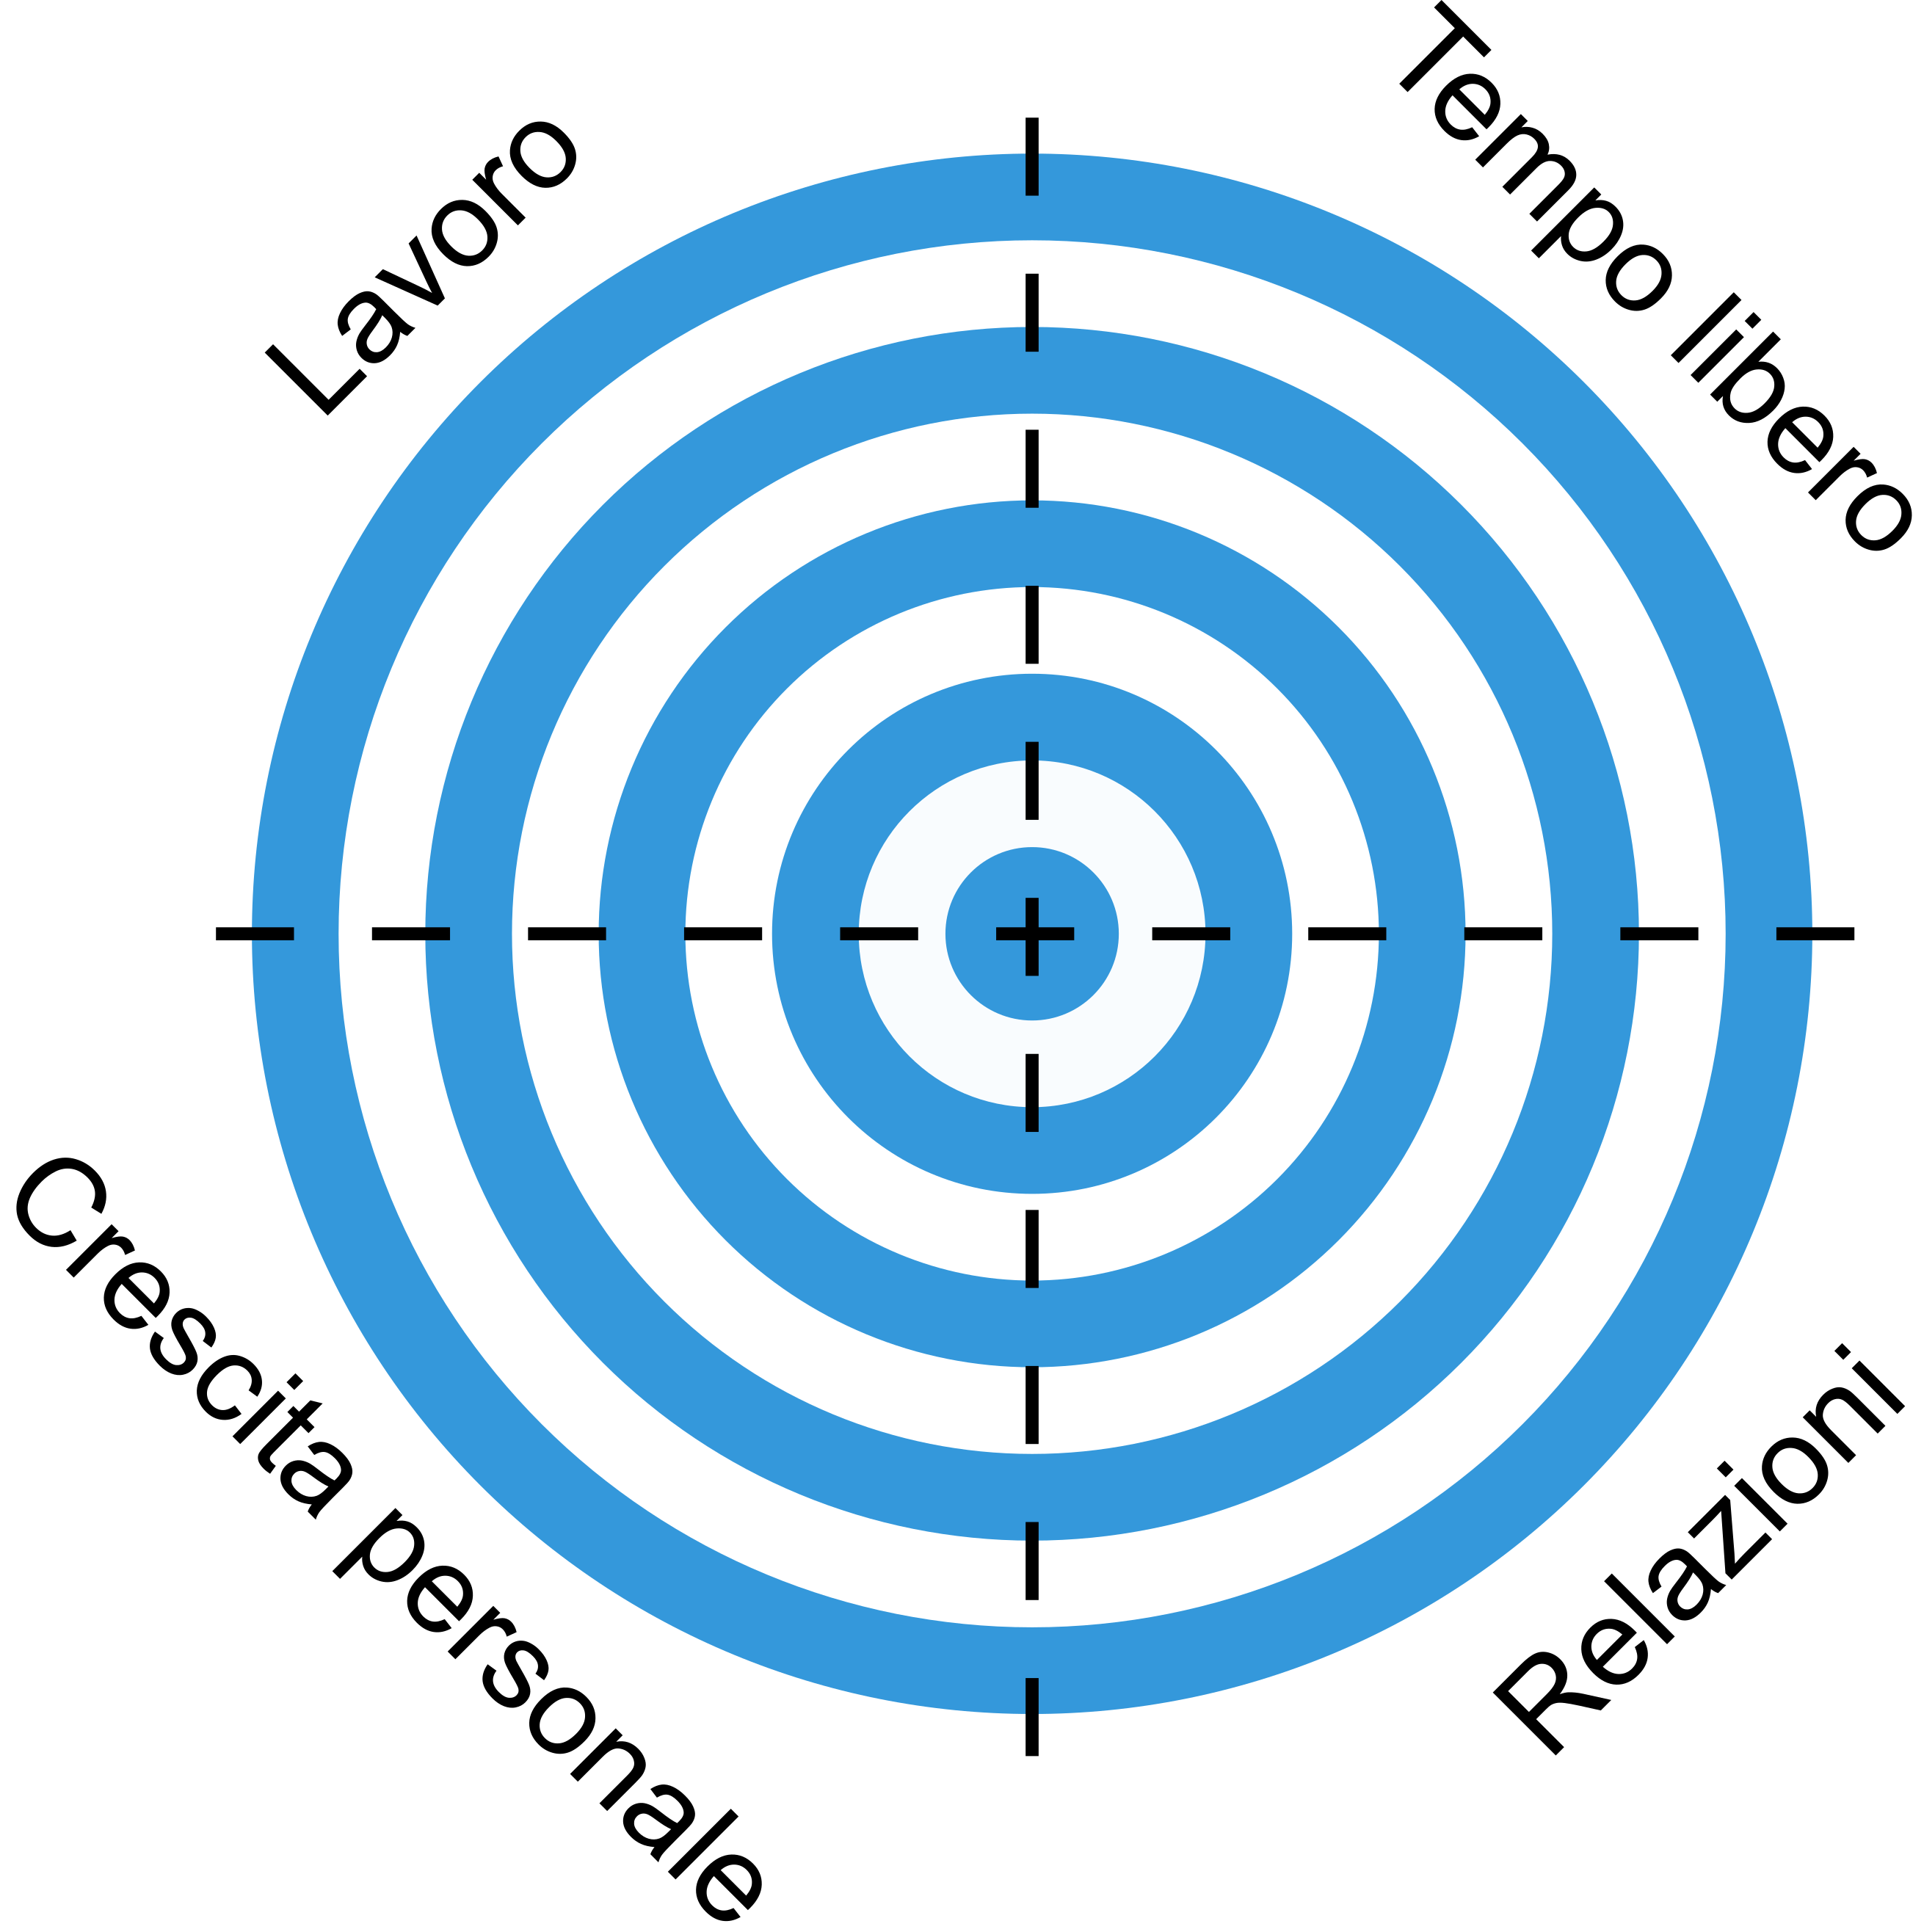
\includegraphics[width=0.95\linewidth]{images/Libro-img014.png}
\end{wrapfigure}

Possiamo fare anche un lavoro che non ci piace e, farlo con piacere se riusciamo a portarci dentro i nostri valori, se
riusciamo a farlo in linea coi nostri valori. I valori giustificano la fatica perché ne vediamo il senso. Se tra i
nostri valori c'è l'ambiente per noi varrà la pena faticare per avere uno
stile di vita più sostenibile. Se nei nostri valori c'è la famiglia, per noi varrà la pena
dedicare del tempo a giocare coi figli. Se nei nostri valori c'è la salute, per noi varrà la pena
lo sforzo di una regolare attività fisica. Non bisognerebbe mai scegliere come obiettivo qualcosa che un morto possa
fare meglio di te, ovvero il non fare qualcosa, come ad esempio smettere di mangiare cioccolata o smettere di sentirsi
depresso. Invece chiediti: se non facessi/sentissi/pensassi più in un certo modo, come impiegherei il mio tempo?

Può però venirci a trovare un demone che ci fa chiedere: “non so se questi sono i miei veri valori”. Possiamo trattare
questo subdolo demone facendoci questa domanda: Se potessi premere un pulsante che ti darebbe la piena approvazione di
tutte le persone che per te contano (quindi non cercheresti di impressionare o compiacere nessuno), cosa faresti della
tua vita e che tipo di persona vorresti essere? Altre volte potremmo chiederci: “Ma i miei valori sono in
contraddizione tra loro”. Può capitare di avere valori che vadano in direzioni diverse, ma non lasciare che questo ti
impedisca di agire, si tratta solo di trovare un compromesso o concentrarsi più su un valore rispetto a un altro, dando
quindi una priorità più alta.

A volte sentiamo che bisogna fare quello che si sente, in maniera spontanea, ed è vero! Ma non basta! Questo pensiero,
presuppone erroneamente tutti gli uomini agiscano in maniera coerente con i propri valori, ma se così fosse sapremmo
già tutti cosa fare per essere felici e lo faremmo. Sappiamo che naturalmente non siamo portati a essere felici, quindi
serve dare una direzione alla nostra vita, con delle regole. Senza regole siamo preda delle passioni, dei desideri
insaziabili, finito uno ne inizia un altro all'infinito. Inoltre, alcune scelte che rappresentano
uno sforzo o qualcosa che non vorremmo fare, possono rivelarsi utili per il futuro, che presto o tardi verrà e ne
potremmo giovare. Una volta che avremmo indirizzato il nostro mondo interiore nella giusta direzione ci sarà un grande
spazio per la spontaneità.

Concentrati sul significato che dai alla tue azioni e, non sulla felicità. Non chiederti cosa ti faccia felice, ma cosa
fornisca senso alla tua vita. La felicità arriverà di conseguenza.

\begin{mdframed}[linewidth=1pt]
Lo studio di Cheung e colleghi nel 2014 voleva spiegare le differenze tra le persone con un buon autocontrollo rispetto
a quelle con un basso controllo. Dallo studio è emerso che la differenza tra questi due gruppi non sta in un intrinseco
dono genetico nel controllo dei propri impulsi, ma di come, questi individui, siano solo più orientati a trovare
strategie per raggiungere i loro obiettivi, piuttosto che essere preoccupati a limitare impulsi che minerebbero questi
ultimi. Quindi il benessere è legato in un certo modo a delle regole, a mettere in atto strategie funzionali,
comportamenti desiderati, ma utilizzando strategie che non riguardano la rinuncia dei piaceri momentanei. Ma come
riuscirsi in un mondo pieno di tentazioni o quando i nostri obiettivi confliggono tra loro? 

Quando riusciamo ad avere delle routine o delle buone abitudini diventiamo in grado di mettere in atto comportamenti
desiderati senza alcun tipo di sforzo in quanto automatiche. Il perseguimento di un obiettivo risulta quindi facilitato
dalla messa in atto di abitudini, piuttosto che dalla soppressione degli impulsi indesiderati, che prosciugherebbero le
risorse di autocontrollo portando al suo fallimento, lasciandoci quindi più energie per le nostre
attività\endnote{\protect\url{https://www.stateofmind.it/2021/05/autocontrollo-impulsi/} }. Anche il prendersi delle pause, seppur
sia vista come una cosa opposta alla produttività, possono invece ridarci nuove energie e farci ritornare più motivati,
se fatte entra una certa misura. In Diventa chi sei\endnote{\protect\url{https://www.amazon.it/dp/B079TLH7PK} }, Emilie Wapnick
consiglia 40 minuti, ma possono essere di più o di meno a seconda della persona. Un altro consiglio per trovare la
motivazione è: iniziare! È proprio vero che chi ben comincia è già a metà dell'opera! 
Uno studio\endnote{\protect\url{https://www.sleepfoundation.org/sleep-hygiene/coffee-nap}} ha confermato che un breve pisolino di 15-20 minuti può essere più efficace del caffè per aumentare l’energia e la concentrazione.
Lo studio “Close, and ye shall find: eye closure during thinking enhances creativity”\endnote{\protect\url{https://www.nature.com/articles/s41599-018-0138-0.pdf}} suggerisce che chiudere gli occhi per due minuti può aiutare a generare idee più divergenti e flessibili aumentando anche la memoria.

Frasi come: trova il lavoro che ami e non lavorerai nemmeno un giorno, non sono del tutto vere in quanto la scintilla,
la musa, la voglia, la motivazione, arrivano e si esauriscono, quello che resta poi è l'essere organizzati,
disciplinati e lavorare. Anche godersi il processo o il viaggio invece del traguardo, va preso in maniera relativa.
Questo perché è improbabile che ci piaceranno tutte le cose del processo e, se dovessimo mettere in dubbio la scelta
del nostro viaggio perché non ci sta piacendo tutto, dall'inizio alla fine, stiamo mettendo delle
basi per la nostra insoddisfazione. Come al solito uno sguardo vanno alle aspettative perché possono frenate la
motivazione. Se io mi dico: devo arrivare la, ottenere quella cosa entro X tempo, potrei non farcela, perché ci sono
fattori indipendenti dal mio agire che possono interferire e demotivarmi, facendoci sentire non all'altezza.

Non esiste una formula che vada bene per tutti. Per qualcuno l'ideale è trasformare la propria
passione in lavoro, mentre per altri è fare un lavoro remunerativo o che lasci abbastanza tempo libero proprio per
poter coltivare le proprie passioni fuori dal lavoro.

Altre volte siamo demotivati perché non riusciamo a completare le cose che ci siamo prefissati. Come spiega Chris
Guillebeau, “[noi] sopravvalutiamo quello che possiamo realizzare in un solo giorno, ma sottovalutiamo quello che
possiamo fare in un anno”. Non hai bisogno della motivazione per fare le cose ma di metodo. Spesso dimentichiamo che la
parola Motivazione è formata da motivo e azione. Un motivo per agire! L'unico modo per essere motivati è iniziare a
fare ciò che volete fare, la passione è molto forte all'inizio ma man mano va a spegnersi e allora
non sarà più quest'ultima a farci muovere ma un metodo, una struttura.

Sulla motivazione ci sono due teorie: 
Dire a tutti dei tuoi obiettivi, così sarai spronato per mantenere la coerenza davanti ai loro occhi.
L'altra teoria invece dice di non dirlo in giro, per evitare che la gente ti demotivi. Queste teorie sono vere entrambe, l'ideale é usare un mix di queste due tecniche e dire i propri obiettivi solo alle persone vicine a noi che sappiamo che non ci feriranno.
Anche le teorie tipo fake it until you make it, ovvero, fai finta finchè non diventa vero, non funziona, anzi, produce l'effetto opposto in quanto immaginare di aver già ottenuto un obiettivo, fa sentire realizzata la nostra mente, come se l'avesse davvero ottenuto e quindi non avrà più bisogno di agire.

Scott Adams dice che per aver successo o sei il migliore di tutti a fare una certa cosa, ma è quasi impossibile, o hai
un set di due o più abilità in cui sei nel gruppo dei 25\% dei più bravi, così da creare una competenza molto specifica
in cui sei tra i migliori. La maggioranza della gente ha come passioni arte e sport, attività difficilmente
convertibili in lavoro, per questo non dovremmo sentirci inadeguati se non riuscissimo a convertire le nostre passioni
in un lavoro.

Secondo Robert J. Vallerand, la passione ha due principali connotazioni: armoniosa o ossessiva. Quelli che provano una
passione armoniosa si impegnano nel lavoro perché ne traggono una gioia intrinseca, e la loro professione convive in
armonia con le altre attività della loro vita. Al contrario, con la passione ossessiva, si ha
un'incontrollabile urgenza di lavorare vivendo in maniera conflittuale la passione e le altre
attività presenti nella loro vita.

La necessità di un lavoro che assecondi le proprie passioni come requisito di una vita ben spesa è un bisogno nato dalla
generazione Y, ovvero quella nata tra gli anni 80 e 2000. Questa ricerca sembra aver portato più stress e
insoddisfazione rispetto alle generazioni precedenti che sceglievano un qualsiasi lavoro potesse dar loro stabilità
economica. Con questo non voglio dire che un lavoro in linea con le nostre passioni sia da evitare, al contrario, ma se
la iniziamo a vivere la ricerca o il lavoro in maniera ossessiva, allora sarebbe preferibile essere costretti in un
lavoro qualsiasi e accettarlo. A volte, come abbiamo visto nel paradosso della scelta: se non hai scelta sei libero.

Per alcune persone è più funzionale dedicare tutta la vita a un progetto, per persone multipotenziali no. Una ricerca
condotta da Bernice Eiduson mostra come nelle 100 pubblicazioni scientifiche tra gli scienziati più famosi del mondo
come Darwin, Feynman, Einstein si trattino mediamente 43 tematiche differenti. Passare da un tema
all'alto, in maniera lenta, dandosi il tempo di approfondire un argomento finché suscita interesse
in noi, che può durare anni, si chiama slow motion multitasking (in quanto il multitasking simultaneo nello stesso
momento, non esiste). Questo saltellare da un tema all'altro, verrebbe visto negativamente, come
una persona con le idee poco chiare. Ma questo ha diversi vantaggi, oltre all'annoiarsi meno,
quello che si apprende in una materia lo si può portare nella risoluzione di problemi in ambiti completamente diversi
e, questa contaminazione, si può anche chiamare in un altro modo:
creatività\endnote{\protect\url{https://www.youtube.com/watch?v=O3YFD9T7fTc} }.

Solitamente viene malvisto lasciare a metà le cose e saltare da un progetto all'altro. Ma dipende
qual è l'obiettivo. Spesso per i multipotenziali l'obiettivo è imparare
qualcosa, quindi quando questo viene raggiunto si passa a qualcos'altro anche se la parte pratica
non è stata ultimata. Sembra che queste persone mollino quando l'attività diventa troppo
complicata, al contrario, questo avviene quando quest'ultima non ha più nulla di stimolante da
offrire. Bisogna stare attenti però a non darsi questa scusa per giustificare la scarsa concentrazione.

Routine, abitudini e creatività non sono infatti in contraddizione. Come diceva Kobe Bryant la creatività ha origine
dalla struttura. Quando hai certi parametri e una struttura, puoi essere creativo al loro interno. Se non hai struttura
fai solo cose a vanvera. Per fare un discorso, ma vale per tutto, difficilmente sarai spontaneo. Se lo prepari bene, puoi usare quello come punto di partenza per fare delle variazioni ed essere spontaneo. Regole e routine alleggeriscono il fardello cognitivo garantendoci lo spazio mentale
necessario alla creatività.

 Se non sei pronto andrai solo a caso, farai confusione e penserai solo a sistemare il casino non permettendoti la spontaneità. E così per tutto. Kobi Bryant diceva che bisogna avere una struttura e da lì si può essere spontanei

Anche nella coppia, le abitudini sono spesso demonizzate. Ricordo un video su YouTube dove Raffaele Morelli racconta di
questa donna sposata che è a conoscenza dell'amante di suo marito. La donna racconta che da
qualche anno, anche lei ha trovato un amante con cui c'è molta passione e molto Eros. Dopo tre anni l'amante di lei le
chiede di diventare la sua compagna e lasciare il marito. La donna però ha preferito continuare a stare con il suo
marito e, si sentiva in colpa di questa decisione, di aver rifiutato l'amante con cui andava tutto
bene, per restare nella vecchia relazione fatta di silenzi. Secondo Morelli invece questa non è una scelta sbagliata,
perché nessuna scelta lo è per la psiche. Se hai fatto quella scelta è perché in quel momento, per la tua crescita, per
la tua maturazione, avevi bisogno di fare quella scelta, poi dal punto di vista pratico, col senno di poi potrebbe
risultare positiva o negativa, ma per la tua psiche era necessaria e giusta proprio quella che hai fatto, eventualmente
per non ripeterla più. Ogni scelta è giusta dal punto di vista psicologico, ma forse, col tempo non si rivela efficace
dal punto di vista pratico ma, non stiamo troppo a pensarci, perché sicuramente, se potessimo tornare indietro nel
passato, con le stesse conoscenze, nella stessa situazione, nello stesso ambiente, faremo le stesse identiche scelte.
La passione non è fatta per durare, mentre le abitudini si. Per questo la signora del racconto ha fatto questa scelta.
Il suo disagio, ancora una volta, non era legato all'evento in sé, ma al giudizio che è stato
dato.

Un altro esempio è la pigrizia. Secondo i ricercatori della Ohio State University analizzando gruppi di studenti che si
rilassavano su un divano, hanno osservato che i partecipanti che pensavano fosse sbagliato impiegare \ il tempo senza
{\textquotedbl}produrre{\textquotedbl} si godevano meno il relax . Al contrario l'idea cambiava se
si pensava che l'attività svolta nel tempo libero potesse portare ad un beneficio a lungo termine. Non è sbagliata
l'attività in sé, ma solo il pensare che sia tempo sprecato è dannoso per la salute. La sensazione
di sprecare il tempo, ci dice qualcosa di fondamentale su di noi, non ci dice qualcosa sulla realtà. Forse non stiamo
vivendo in linea coi nostri valori o forse il nostro giudice interno è troppo esigente. Semplicemente notatelo. Non
fare niente non è mai fare niente: ti obbliga a riflettere e a compiere libere associazioni, che si possono rivelare
utili\endnote{\protect\url{https://www.vice.com/it/article/xgxy8w/noia-tempo-libero-pietro-minto} }.
\end{mdframed}

Il nostro benessere e la nostra felicità dipendono da come interpretiamo la realtà, che significato e definizione gli
diamo e quali aspettative avevamo a riguardo. Noi non possiamo vedere la realtà, ma solo interpretarla e come ogni
interpretazione la deformiamo, coi bias che abbiamo visto nel primo capitolo e con perdita di significati e
particolari. Le parole sono il linguaggio del nostro pensiero. Utilizzare delle parole invece di altre comporta,
comporta, a livello emotivo, una significato piuttosto che un altro.

Persone che parlano in modo diverso della stessa cosa, vivono in modo diverso e la realtà per loro è diversa. c'è
differenza infatti tra dire:\newline
“che freddo” o “si congela”\newline
“ho mal di testa” o “mi scoppia la testa”\newline
“sono stanco” o “sono distrutto”\newline
“mi urti” o “mi fai uscire di matto”

Le parole ci suggestionano. Se diciamo “non ho mai tempo” non riusciremo a introdurre nulla di nuovo nella nostra vita.
Se siamo abituati a dire spesso “sono stanco”, tenderemo a sentirci stanchi davvero. Questo perché possiamo
concentrarci solo su una cosa per volta e ci concentriamo solo sulla stanchezza isolandoci da ogni altro aspetto che,
comunque, resta presente, ma perde importanza. Così come dire “sei pallido...” o “ti senti bene?” ci fa concentrare
sulla presenza di problemi, spesso aggravandoli. Anzi, Fare una cosa alla volta è un modo straordinario di meditare e
di restare consapevoli. Gli studi dimostrano che basterebbe diventare {\textquotedbl}consapevoli{\textquotedbl} di
circa 20 respiri al giorno per migliorare la nostra concentrazione, la nostra calma e il nostro benessere sotto molti
punti di vista.

Altro esempio, dire: “non sono capace” porta con se una giudizio, un limite, che porta alla “profezia che si
auto-avvera” rendendoti davvero incapace di compiere quella cosa. Mentre dire “non sono ancora capace” da una
potenzialità completamente diversa all'atto che stai per compiere. Molto ricerche hanno dimostrato di come la profezia
che si auto-realizza funzioni meglio in negativo che in positivo, quindi ha molto più effetto quando ci scoraggiamo
rispetto a quando ci incoraggiamo. Alcuni filoni di pensiero ottimista, auto aiuto ecc… utilizzano molto le frasi
motivazionali e dirsi che va tutto bene. Oggi sappiamo che queste tecniche non sono efficaci in quanto, le suggestioni,
funzionano meglio se sono inconsce (l'effetto placebo ne è un esempio). Quando utilizziamo
volontariamente il pensiero positivo, avviene un effetto paradossale, ovvero: Se sono triste e mi sforzo di pensare
positivo, la sensazione resterà ma, non essendo in linea con il pensiero, la mente vedrà questo come un problema e,
come sappiamo, il compito del cervello è risolvere i problemi. Questo ci porterà a chiederci cosa
c'è di sbagliato in noi, cosa dovremmo cambiare e altre domande potenzialmente disfunzionali. Il
pensiero positivo, che all'apparenza sembra una buona idea, porta all'effetto
opposto, peggiorando lo stato d'animo. Anche qua, torna prepotentemente la via di mezzo: pensare
ai propri disagi è sempre sbagliato? Ovviamente no, magari la tristezza è nata per portarci a cambiare qualcosa, altre
volte invece va tutto bene, ma sono le nostre domande a farci diventare tristi, sopratutto quando ci concentriamo su
quello che non abbiamo e che magari è un desiderio indotto dall'esterno.

La “positività tossica” si riferisce alla convinzione che si debba mantenere un atteggiamento positivo e ottimista in ogni situazione, ignorando o svalutando le emozioni negative. Uno studio condotto dalla Tilburg University\endnote{Perceiving societal pressure to be happy is linked to poor well-being, especially in happy nations\protect\url{https://www.nature.com/articles/s41598-021-04262-z}} nei Paesi Bassi, che ha coinvolto 7.443 persone provenienti da 40 diversi paesi, ha esaminato l’impatto della pressione sociale per la felicità sul benessere individuale.
Il paradosso scoperto è che l’incoraggiamento sociale a mantenere un atteggiamento positivo può avere effetti negativi, portando a esperienze di emozioni positive meno frequenti e meno intense, mentre intensifica quelle negative. L’idea di dover essere costantemente felici, che è irrealistica, può far sentire le persone inadeguate e l’atto di reprimere le emozioni negative può paradossalmente intensificarle.

Ellen Langer ha condotto un esperimento con degli anziani. La ricercatrice ha condotto diverse misurazioni sulla
pressione sanguigna, ossigenazione del sangue, frequenza respiratoria, livelli di attenzione, ansia, benessere ecc...
poi li ha portati in un villaggio a tema anni 60 e, ha chiesto loro di parlare al presente, come se fossero davvero gli
anni 60, con i modi di dire, le situazioni, vestiti, insomma comportandosi e facendo tutto come se fossero ritornati
indietro nel tempo. Dopo un periodo ha ricondotto le misurazioni sugli anziani e ha notato un miglioramento generale.
Alcuni di loro, privi di qualsiasi potere decisionale sulla propria vita, non avevano nemmeno il controllo su ciò che
mangiavano. Tuttavia, una volta che è stata loro concessa la possibilità di prendere decisioni su alcuni aspetti della
propria esistenza, si è notato un ulteriore ringiovanimento nelle misurazioni. Gennaro Romagnoli infatti sostiene che
la qualità della vita è strettamente legata alla propria
curiosità.\endnote{\protect\url{https://ichgcp.net/it/clinical-trials-registry/NCT03552042}}

Pensate alla differenza, in una conversazione, di queste due espressioni: “non hai capito” o “mi sono spiegato male”.
Nella prima forma una persona suppone di essersi spiegata bene e che il problema sia l'altro, ma non ne ha nessuna
certezza, mentre nel secondo caso, si mette in dubbio la propria esposizione invece della comprensione dell'altro.

In realtà le cose, la vita, le persone sono quello che sono ma il modo in cui noi le definiamo cambia completamente la
nostra esperienza. Abbiamo visto sia irrealizzabile cercare in una relazione di coppia, anche dopo molti anni, le
emozioni dei primi mesi. Ma se noi definiamo come “amore” i sentimenti dei primi tempi, potremmo interrogarci sul fatto
che non amiamo più. Se dopo diverse relazioni ci troviamo a fare sempre la stessa domanda potremmo arrivare a
interrogarci sul fatto di non essere in grado di provare amore. O la “felicità”. Se trovo la felicità sarò terrorizzato
dal perdere le condizioni che mi ci hanno portato. Se pensiamo che una volta ottenuta la stabilità economica, una
compagna o un compagno, un lavoro, famiglia e figli otterremo una felicità perpetua, immutabile, senza più provare
tristezza, ecco che stiamo dando alla felicità un significato irrealizzabile. Ma noi continueremo a cercare quella
felicità impossibile che ci causa frustrazione. Noi diventiamo tristi appena pensiamo di essere tristi, anche se non lo
siamo veramente. Siamo tristi appena nascono pensieri di tristezza e il nostro dialogo interiore continua a parlare di
questa tristezza, alimentandola.

Non siete sbagliati voi, gli altri, la vita, le circostanze, semplicemente in quel momento, vi sentite così, ne prendete
atto e lo accettate, consapevoli che tutto passa e che potreste sentirvi tristi della tristezza, aver paura della
paura, più che della tristezza o della paura in se. Siete afflitti per il giudizio che queste cose non dovrebbero
andare così, per la definizione che avete dato di come dovrebbero andare le cose. 

La felicità dipende anche da aspetti legati alla cultura ed al posto in cui viviamo. In Nordamerica la felicità viene
definita con la realizzazione personale (compreso il piacere), mentre in Asia orientale la felicità è associata
all'armonia sociale. Gli americani di origine cinese preferiscono
l'appagamento, mentre, gli americani di origine europea preferiscono
l'eccitazione.\newline
Essere felici in una determinata cultura dipende tanto da quanto le vostre emozioni sono sincronizzate con la
definizione di felicità espressa in quel contesto sociale. 

Le parole che utilizziamo, le definizioni, sono una “sintesi” una “mappa” della realtà, che portano con se una perdita
di significato e cancellazione di dettagli. Le parole le usiamo per comunicare ma anche per pensare, per definire noi
stessi e quello che secondo noi dovremmo provare. Ma la realtà è quello che è, indipendente e slegata dalle definizioni
e da come la vogliamo incasellare o dagli un senso. Provate a descrivere il profumo di una rosa. È impossibile, seppur
non sia un concetto astratto, per cui immaginatevi descrivere dei sentimenti. Per questo quando ci sentiamo inadeguati
o che dovremmo provare certe emozioni in certe situazioni non possiamo essere certi di cosa stiamo cercando in questo
“dovere” che dovere non è. È solo quello che secondo noi dovrebbe essere, ma in base a cosa? Su quale principio morale
dobbiamo essere sempre allegri ad esempio? Perché dovremmo sentirci inadeguati se non lo fossimo? Inoltre il nostro
mondo è filtrato dai nostri cinque sensi, lo percepiamo attraverso di loro. Immaginate di spiegare a un cieco il colore
verde, è impossibile. Questa persona probabilmente ci chiederà: è caldo o freddo? Grande o piccolo? Ruvido o morbido?
Non ha gli strumenti per comprenderlo. Immaginatevi, allo stesso modo, di essere in un mondo teorico dove alcuni
animali hanno un sesto, settimo, ottavo senso. Avrebbero un'accresciuta e più profonda percezione
delle cose, che loro non potrebbero riuscire a spiegarci in nessun modo e noi non potremmo capire, per noi è come se
non esistessero, ma esistono e, magari, queste informazioni ci chiarirebbero dei misteri su come percepiamo la nostra
vita, esteriore e interiore. Questo è il limite delle parole. 

Quando il saggio indica la luna lo stolto vede solo il dito (proverbio cinese). 

Allo stesso modo, pensiamo alle persone. A parità di situazione uno può reagire con euforia un altro con ansia, uno con
eccitazione l'altro con paura e, per quella persona quel sentimento è reale, non è meno vero di un
altro, anche se la situazione è la stessa per tutti. Una persona che viene calata in un burrone e ha paura del vuoto
sta vivendo davvero un terrore puro, nella sua testa c'è un reale rischio di cadere, è irrazionale
siccome è legato e, quella persona forse lo sa anche, ma ciononostante non può smettere di avere paura di una cosa che
non esiste. Cosa cambia allora da persona a persona? La mente! O meglio lo storytelling, la storia che ci raccontiamo
mentalmente attorno a quella situazione, per esempio il cambio di lavoro, può \ portare a pensieri stimolanti, si
acquisiscono nuove conoscenze, nuove esperienze, nuove persone ma per qualcun altro sorgono pensieri di preoccupazione,
ansia, di non essere all'altezza della situazione, tutte cose giuste. Anche la persona con ansia
sarà appagata e gratificata dalle nuove capacità che acquisirà, solo che non pensa a quello inizialmente. Allo stesso
modo, l'altra persona si troverà a fare cose che non conosce e, sarà stressante, frustrante, solo
che prima non ci aveva pensato e non ci soffriva. Non è sbagliato prepararsi al peggio, anzi, ci permette di gestire
meglio la situazione quando e se si presenterà. 

Se soffri di vertigini fai un corso di arrampicata, convivendo con l'altezza pian piano diventerà
la norma e, non farà più paura, allo stesso modo puoi fare con i tuoi sentimenti.


\bigskip

Amore e felicità sono solo due parole che possono essere fuorvianti, ma in modo diverso ne abbiamo altre, ancora più
comuni come; niente, mai, sempre, ogni volta ecc.. Quante volte usiamo le frasi: “non facciamo mai NIENTE”, “la casa è
TUTTA in disordine”. Queste parole sono chiamate “quantificatori universali”. Nel modo di parlare comune equivalgono al
classico modo di dire: “fai di tutta l'erba un fascio”. Quando utilizzi queste parole stai
cancellando dettagli e parti della realtà e ti allontani dal tempo presente. Cambiare un modo di parlare, uno schema
mentale per costruire le frasi e di conseguenza il mondo interiore che utilizziamo nel nostro dialogo interno coi
pensieri, non è una cosa facile. Ma dovremmo interrogarci, per riportare l'attenzione nel qui ed ora, con domande tipo:
“sono proprio sicuro che sia sempre/mai/tutto così? Ci sono state volte in cui non è andata così? o forse sto
esagerando”?

Se la casa ogni tanto non è in ordine come vorremmo, ma ormai ci siamo abituati a dire che è SEMPRE in disordine, allora
nella nostra mente, per la nostra realtà, la casa sarà SEMPRE in disordine. Quello che noi ci diciamo è la nostra
realtà. Se per noi poi avere la casa in ordine è una cosa importante, non saremo felici. Non saremo felici per una cosa
non vera.

Trovare continuamente difetti sul proprio aspetto fisico, per esempio dire delle proprie mani: “sembrano quelle di un
vecchio” oppure dire “sono con me da tutta la vita e grazie a loro ho fatto un sacco di cose” farà vivere queste due
persone in una maniera completamente diversa. Questo può succedere per tutto, il lavoro, il meteo, i suoceri, genitori,
figli. Nella cultura giapponese esiste il Kintsugi, ovvero l'arte di esaltare le ferite, che nasce
dalla necessità di riparare un vaso rotto. Gli artigiani non buttarono via i cocci e non realizzarono una nuova copia,
non cercarono nemmeno di nascondere le crepe, ma anzi, le resero molto più visibili e preziose utilizzando
dell'oro. La tradizione del Wabi-sabi si oppone al concetto di perfezione come uno risultato di
una bella vita, piuttosto il concetto si riferisce nell'apprezzare le imperfezioni che
inevitabilmente fanno parte della nostra esistenza. Wabi-sabi può anche voler dire apprezzare il tempo che passa, le
rughe e la saggezza. Il concetto rileva anche come l'imperfezione aggiunga un ulteriore livello di
significato\endnote{Ikigai, Kaizen, Shinrin-yoku, Kintsukuroi \protect\url{https://www.amazon.it/gp/product/B0992X391K} }.

Il verbo essere, quando usato come predicato nominale, può essere pericoloso. Porta con sé la certezza di qualcosa, una
definizione, regole, limiti e omissione di dettagli. Meglio riformulare la frase in una domanda rispetto ad una
affermazione, lasciando così aperto un dubbio, una possibilità, lasciando la mente più libera ed elastica. Avere
certezze su tutto da sicurezza ma vi rinchiude in una gabbia che voi stessi vi siete costruiti. La vita e noi stessi è
costantemente in cambiamento, mentre il giudizio fotografa e blocca. La complessità dell'essere
umano rende impossibile ogni certezza semplificata in un giudizio, per cui le mie idee sulle persone, le cose e i
sentimenti sono sempre ipotetiche e, pronte ad essere modificate.
Se non sai cambiare idea, se sei dogmatico, rischi la disonestà intellettuale che ti porterà a giustificare sempre le tue convinzioni con menzogne. E sarà stressante continuare a mentire e a ricordare le menzogne dette. Possiamo giudicare il comportamento, ma non la
persona tra cui noi stessi. Anche perché troppo spesso siamo moralisti fino a quando non ci troviamo nella stessa
situazione. Questa potrebbe essere la buona occasione e servirci da spunto per smettere con tutti i moralismi, invece
smettiamo solo con quel particolare giudizio. Se siamo persone che hanno la tendenza a criticare gli altri
probabilmente critichiamo anche noi stessi, magari su altre cose, magari sulle stesse. Quindi può essere un campanello
per accorgerci che abbiamo la tendenza a giudicarci. Non dovremmo etichettare negativamente o come insicuro chi cerca i
plausi, ma riconoscere che tutti noi abbiamo queste tendenze umane in modalità diverse. Questo della sicurezza è solo
un esempio, pensiamo ad ogni critica e notiamo che possiamo applicare questo ragionamento.

Possiamo giudicare le azioni, ma non le persone, non ne abbiamo il diritto. Possiamo additare un pedofilo, un assassino
come un mostro e poi scoprire che per anni, nell'innocenza di bambino che è stato, senza colpe, ha
subito le peggiori violenze. Nei giusti contesti anche noi potremmo essere dei mostri come abbiamo visto
nell'esperimento del carcere di Stanford e in quello della terza onda. Bisogna avere compassione
delle persone che compiono errori, perché mostriamo compassione verso noi stessi, verso quell'io
in un altro corpo, in altre circostanze.

Le parole che definiscono sono sentenze.

Quando giudichiamo qualcosa lo definiamo. La parola definire deriva dal latino e significa limitare, stabilire dei
confini. Quando noi definiamo qualcosa o qualcuno stiamo stabilendo delle regole sui suoi confini, stiamo limitando ciò
che è o può essere. In altre parole, stiamo confinando qualcuno o qualcosa a una definizione molto stretta che fa da
trappola sia per noi che per lui/lei. Pensa a quando la gente ti chiede che lavoro fai. Automaticamente tu diventi
quella cosa, quel ruolo, quella funzione. Alle soglie del pregiudizio.

Quando io definisco una persona in qualche modo è perché, dentro di me, mi sono messo dalla parte del giudice, ho emesso
una sentenza (la definizione) e l'ho condannata a delle conseguenze (il mio comportamento nei suoi
confronti). E lo facciamo per ogni cosa, non solo le persone, tra cui anche noi stessi. Noi siamo quello che siamo,
indipendentemente dai giudizi, ma definendoci non ci stiamo dando la possibilità di esserlo. Per questo ogni tanto ci
sentiamo inadeguati verso certe situazioni, verso noi stessi, verso gli altri o i sentimenti. O meglio, ci sentiamo
inadeguati verso il giudizio, la sentenza, la definizione che abbiamo dato a tutte queste cose, che per come le abbiamo
poste sono impossibili. Ci sentiamo inadeguati verso come impossibili.

Non sempre però le persone si comportano in maniera giusta vero? Certo, se una persona picchia, ruba, uccide ecc… non
abbiamo dubbi, sono forti privazione della proprio volere e della propria libertà. Prendiamo però
l'esempio di una persona che arriva in ritardo. Noi ci diciamo che è una mancanza di rispetto per
il nostro tempo, perché noi siamo arrivati puntuali e siamo stati costretti ad aspettare, senza poter fare niente,
annoiandoci, se avessimo saputo che ci fosse stato questo ritardo potevamo stare a casa a finire di fare alcune cose
ecc… Scrivo spesso che ogni scelta è giusta se non limita la libertà altrui, in questo caso io potevo fare un sacco di
altre cose e invece sono costretto a stare qua da solo ad aspettare i comodi di questa persona, quindi lei ha
sbagliato! Ma è davvero così? Questa persona non ci ha messo delle catene, noi potremmo mandare un messaggio e
scrivere: Troviamoci in libreria, così intanto guardo se è uscito quel libro che cercavo, o altrimenti, io entro al
cinema, così non mi perdo l'inizio e te lo racconto, ecc… Quindi perché rimaniamo lì ad aspettare,
immobili, pieni di pensieri su come tutto questo sia sbagliato? Perché se abbiamo una scelta non facciamo niente?
Perché le nostre definizioni ci dicono che, primo, si arriva all'orario prefissato e secondo, \ si
aspetta nel punto prestabilito. Non abbiamo delle catene fisiche, ma catene mentali, anche se il risultato però è lo
stesso. Con questo non voglio dire che sia giusto arrivare in ritardo, ma dico che se potessimo entrare nella testa
della persona, probabilmente lei voleva arrivare in orario, ci ha provato in tutti i modi, non voleva farci rimanere
male in nessun modo, ma purtroppo non c'è riuscita e magari non ci riesce mai. Troviamo studi
anche su questo e ci sono diverse motivazioni. Tra le teorie più diffuse sembra che alcune persone non abbiano una
buona memoria temporale e percepiscono lo scorrere del tempo in maniera diversa. Quindi per esempio, quando si
preparano, se impiegano venti minuti hanno la percezione di averci messo meno tempo e, stesso discorso per il viaggio
in macchina, portandole a sottostimare tutti i tempi e ad arrivare così in ritardo. Qualunque sia la motivazione,
proviamo a vedere la cosa da un punto di vista esterno, freddo e razionale: se una persona a piacere ad uscire con voi
che ragioni avrebbe di farvi del male? E perché, ogni volta che ci siamo trovati ad aspettare abbiamo fatto mille
pensieri, sempre lo stesso in realtà e non abbiamo mai pensato a questo aspetto? Perché il nostro schema mentale
produce sempre le stesse soluzioni ad un problema, non prova altre strade se non ci alleniamo a farlo. Se sappiamo che
non era intenzione della persona farci stare male, avremmo ancora buone ragioni per avercela con lei? In realtà quando
siamo sereni, stiamo bene, anche se l'intenzione fosse stata quella di ferirci, non ci arrabbiamo,
quindi indipendentemente dall'intenzione dovremmo sempre gestirla così, come se la persona che
abbiamo davanti non volesse ferirci. Rispondiamo senza dare bacchettate sulle mani, ma magari in modo spiritoso tipo:
ok brontolo o, va bene mamma :) .

Ora io ho fatto l'esempio del ritardo, ma se ne potrebbero fare tantissimi altri. Per trovare
l'esempio giusto per voi, ripensate a tutte le volte che pensate che avete subito un ingiustizia o
che qualcuno si sia comportato male con voi. Provateci davvero a fare questo esercizio. Troverete anche cose
oggettivamente ingiuste, ma la gran maggioranza saranno cose che avete vissuto come sbagliate. Ora però provate a
cercare le motivazioni che hanno portato quella persona a fare quella cosa, probabilmente non troverete il volervi
ferire.

Verrebbe quasi da pensare che il cervello sia fatto male. Sembra che ogni cosa li dentro sia fatta per farci fare male.
In realtà non è così, se rinunciamo a questi effetti negativi del cervello dovremmo rinunciare anche a quelli positivi.
L'apprendimento per esempio, da cui deriva ogni cosa che sappiamo fare, da camminare, parlare, e
costruire. Noi impariamo per esempi, ma siccome non possiamo memorizzarli tutti, riusciamo ad astrarre in modo da
creare un regola generalizzata per gestire e risolvere un particolare problema. Quando parlo di problemi non parlo
necessariamente di avversità. Per esempio per la comunicazione può essere vista come il problema da risolvere e la
parola lo strumento per risolverla. Quindi la generalizzazione, che sta alla base
dell'apprendimento può portare ad alcuni problemi. Ad esempio posso imparare che una persona che
alza la voce mi stia aggredendo, o mi voglia zittire, quando invece lei lo sta facendo solo perché
l'argomento trattato la coinvolge molto a livello emotivo. Addirittura posso generalizzare ancora
di più e un singolo episodio, dove una singola persona alza la voce, nella mia generalizzazione possa diventare: Tutti
mi odiano sempre! E se ci penso su troverò sicuramente altri episodi dove ho avuto la sensazione che qualcuno mi
trattasse male, in modo da dare forza a quel “tutti” e quel “sempre”.

Se ad esempio proviamo qualcosa e non ci piace, ne proviamo un altra e non ci piace, al terzo tentativo fallito il
cervello inizierà a generalizzare e definirsi come una persona a cui non piace niente, senza interessi, senza stimoli o
che non riesce in quello che sta facendo o qualsiasi altra cosa. I giudizi derivano anche dalla generalizzazione ma
anche l'apprendimento funziona per generalizzazione. Quindi? Siamo condannati
all'infelicità? Non c'è via d'uscita? No, ma se sappiamo
come funziona la nostra mente e diventiamo consapevoli dei giudizi, degli schemi mentali, dei bias, dei condizionamenti
ecc… non ne siamo più in balia. Ogni volta che sentiamo un giudizio dobbiamo allenarci a dire: ecco, la mente mi sta
criticando per i motivi che abbiamo visto durante questa lettura, prenderò in considerazione quello che mi dice in un
secondo momento, in ogni caso non mi sta dicendo che sono sbagliato, però ora ritorno a fare quello che stavo facendo e
poi lo valuterò, con alcuni esercizi che vedremo tra poco, come la scrittura espressiva, la meditazione, la ricerca del
bisogno che ha fatto scattare la critica ecc…

In particolare, quando ci sentiamo senza stimoli forse stiamo facendo troppe cose, stiamo producendo troppo output,
quindi da noi verso l'esterno e, non stiamo ricevendo abbastanza input, quindi cose che
dall'esterno entrano dentro di noi, come viaggi, libri, film ecc... 

Se ora ci ritroviamo in queste parole e vorremmo cambiare, ci stiamo dando ancora una volta una definizione. Ci sentiamo
sbagliati e secondo noi, secondo il nostro giudizio, dovremmo cambiare. Non è consigliabile forzare se stessi e farsi
violenza, dobbiamo cercare di essere ciò che siamo e eventualmente cambiare coi giusti tempi. La mindfulness e la
meditazione servono a non cambiare niente limitandosi ad osservarlo, senza intervenire, accettando senza giudicare i
propri lati di se, anche quelli che ci piacciono meno. Questo non vuol dire sedersi sulle proprie cattive abitudini
giustificandosi dietro la frase “sono fatto così, non ci posso fare niente”. Se noi riconosciamo di avere un certo lato
di noi, accettiamo che esiste, ne siamo consapevoli, con il tempo ci accorgeremo quando emerge e, giorno dopo giorno,
senza che interveniamo intenzionalmente, ma in maniera del tutto spontanea e naturale, vedremo un cambiamento.

Quindi, la prossima volta, tra pochi secondi, che etichetterai qualcosa o qualcuno con qualche definizione, non fare
niente. Semplicemente annotalo, osservalo, prendine atto, sii
testimone\endnote{\protect\url{https://www.maxfuria.com/le-parole-che-ti-cambiano-la-vita-e-quelle-che-la-peggiorano/} }
\endnote{\protect\url{https://amico-in-affitto.com/2017/08/14/le-parole-che-cambiano-la-vita/} }.

\begin{mdframed}[linewidth=1pt]
Nel libro l'illusione della memoria\endnote{\protect\url{https://www.amazon.it/dp/8868334313} } di Julia Shaw abbiamo numerosi esempi
e spiegazioni di come, il nostro principale oggetto riguardante la nostra identità, sia fallibile. La nostra mente
potrebbe ricordare delle cose mai vissute e tutti facciamo esperienza di questo errore, solo che non possiamo saperlo.
Sembra infatti impossibile avere ricordi avvenuti prima dei nostri 3 anni di età, eppure tutti o quasi potremmo giurare
di aver delle immagini di quel periodo. Ma com'è possibile? Questa tipologia di memorie si
chiamano ricordi indotti. Probabilmente i nostri genitori ci hanno raccontato di quell'episodio,
magari mostrandoci anche delle foto e, mentre parlavano, la nostra mente ha iniziato a produrre delle immagini; anche
perché non riuscirebbe a fare altrimenti, esattamente come quando si dice di non pensare ad un elefante bianco. Siccome
quel racconto riguardava noi, l'abbiamo fatto nostro. La memoria infatti non è consultabile
direttamente, ma solo attraverso l'area dell'immaginazione. Ogni volta che
vogliamo accedere ad un ricordo lo dobbiamo immaginare e, questo processo, deforma anche i nostri veri ricordi. Più
ripensiamo ad un episodio e più lo deformiamo. Un esperienza non è traumatica di per sé, ma solo quando la etichettiamo
come tale. Se una persona vive un trauma e riesce a gestirlo bene, se si confrontasse con altre persone che hanno
vissuto la stessa esperienza e sono in lacrime, questa persona potrebbe rivalutare il giudizio dato all'esperienza. Un
modo per avere ricordi più veritieri è quello di tenere un diario e rileggerlo periodicamente.

Anche la nostra memoria è vittima di numerosi bias. Infatti tendiamo a lasciare nella nostra memoria una traccia
maggiore circa le cose positive che facciamo. Per questo molte persone pensano di essere più brave a guidare rispetto
alla media, o più intelligenti o più attraenti o di fare più faccende domestiche rispetto al nostro partner. I
poliziotti pensano di saper individuare un criminale, un insegnante di essere chiaro nelle spiegazioni e, gli studenti
di aver capito tutto. \ Se tutti pensano di essere sopra alla media, la maggioranza si sta sbagliando e, questo è
impossibile.

Uno di questo bias si chiama bias di sopravvivenza, ovvero ricordare meglio i successi dei fallimenti. Se pensiamo a
Steve Jobsh, Mark Zuckerberg e altri, che hanno lasciato l'università e hanno avuto successo, possiamo pensare di farlo
anche noi, ignorando a quante persone invece è andata male. Stesso discorso vale per gli investimenti economici. Quando
ci si trova davanti a qualcosa di miracoloso, per la nostra salute fisica, mentale, finanziaria potremmo essere
entusiasti per questo motivo, perché non appuriamo chi invece ha fallito. Ogni volta che mi è stato proposto qualcosa
rivoluzionario sono sempre rimasto molto deluso e, ha senso, altrimenti lo farebbero tutti.

Queste nuove scoperte stanno minando diverse tecniche che sono durate fino ad oggi. Ad esempio
l'ipnosi, utilizzata per accedere a ricordi rimossi, oggi si teme che possa invece generare nuovi
falsi ricordi. Anche nella psicoanalisi, se il terapeuta ti fa immaginare un ricordo traumatico potrebbe creare una
falsa memoria. Anche certe modalità di interrogatorio, possono addirittura portare una persona innocente a credere di
aver commesso anche cose gravi, come un omicidio o uno stupro. \ Esami del DNA hanno smentito numerosi confessioni di
testimoni oculari.

Julia Shaw spiega come la generazione di ricordi richieda attenzione, quindi l'autosuggestione
passiva o ascoltare audio mentre si dorme per rendere lo studio meno faticoso, si dimostrano strategie inefficaci.
Anche i giochi per migliorare la memoria sembrano non funzionare. La ricercatrice spiega anche come la percezione del
tempo sia influenzata dalla memoria. Se abbiamo tanti ricordi di un certo periodo, la percezione che abbiamo è più
lunga rispetto a quando abbiamo pochi ricordi. Il picco delle reminiscenze e il maggior numero di ricordi si colloca
attorno ai 20 anni, in particolare tra i 10 e i 30, dopo il tempo sembrerà correre più velocemente. Inoltre spiega
perché alcune persone sono spesso in ritardo. Probabilmente dipende queste persone non hanno buona memoria prospettica.
Non ricordano quanto ci hanno messo l'ultima volta a prepararsi per esempio, faticando a pianificare il futuro in base
a esperienze pregresse.
\end{mdframed}

In questo modo noi possiamo ripensare al passato e al futuro, utilizzando parole diverse e ridefinire ciò che siamo,
cambiando noi stessi, portando l'attenzione solo su certe storie. 

Le ricerche svolte, infatti, dimostrano che quando pensiamo al futuro lo facciamo in maniera
negativa\endnote{\protect\url{https://science.sciencemag.org/content/339/6115/96} }. Mentre secondo le ricerche di Oliverio, in
“Immaginazione e Memoria“\endnote{\protect\url{https://amzn.to/3eZJT15} } quando ricordiamo il passato, non sono gli eventi
realmente accaduti, ma quello che ci raccontiamo degli accadimenti. Le parole come studiato dallo psicologo Jerome
Seymour Bruner, sono influenzate dal nostro cervello e, a sua volta, il cervello e la cultura sono influenzate dalle
parole che si dicono e che si
ascoltano\endnote{\protect\url{https://www.amazon.it/fabbrica-delle-storie-Diritto-letteratura/dp/8842080926} }.

Se hai poca autostima non sei contento ma se ne hai molta devi continuamente mantenerla con la paura di perderla. Come
sarebbe la tua vita senza autostima e i relativi giudizi di come dovresti essere? Questa idea non basterà a bloccare la
tua mente dall'emettere giudizi, ma li vedresti semplicemente per ciò che sono, semplici pensieri.

\begin{mdframed}[linewidth=1pt]
Un giorno Jean-Paul Sartre si ruppe una gamba durante un'escursione in montagna. In ospedale venne
il suo amico Merleau-Ponty a fargli visita e gli chise: “Ma non potevi farti accompagnare da una guida?”. Sartre
risposte: “Io sono Jean-Paul Sartre! Mi ci vedi ad andare in montagna con una guida?”. Se fosse stata
un'altra persona, con un'altra identità, si sarebbe potuto concedere
un'escursione con la guida, ma per il suo personaggio, questa non era tra le sue possibile scelte
ipotetiche. L'identità quindi diventa il limite dei limiti e riduce le nostre scelte e la sua
conseguente libertà. Al contempo però la società si regge solamente se gli individui hanno
un'identità. La società infatti regge se tutti rispettano le regole, se nessuno uccide, se nessuno
ruba e noi, società, ci aspettiamo che gli individui si comportino così, che non abbiano certe libertà, perché la loro
personalità glielo vieta, la legge infatti può intervenire solo se una ristrettissima cerchia di individui non riesce a
integrarsi. Il cerchio si chiude in quanto un individuo non può sopravvivere, anche emotivamente, senza un gruppo di
appartenenza. Noi abbiamo bisogno di un gruppo, il gruppo ha bisogno di sapere che noi non faremo certe cose, la nostra
identità individuale e di appartenenza, siccome dobbiamo sopravvivere aggiunge certe regole. 

Anche qua possiamo trovare la via di mezzo. Possiamo andare contro tutte le regole sociali purché non danneggiamo gli
individui o l'ambiente. Consapevoli, che alcune nostre scelte, seppur rispettino
quest'ultima regola, potrebbero non venire accolte da alcuni individui e potrebbero allontanarci,
ma è anche vero però, che il mondo è così grande e vario che ci sarà sicuramente un gruppo che la pensa come noi.

L'uomo civile ha barattato una parte della sua possibilità di felicità per un po' di sicurezza - Sigmund Freud.
\end{mdframed}

Concludo dicendo che il giudizio non è il male. Il giudizio è necessario per valutare e prendere decisioni. Anche qua,
non a caso, serve una giusta via di mezzo. Dovremmo astenerci sempre dal giudizio inconsapevole, quello che parte senza
che l'abbiamo scelto noi. Cerchiamo di diventare consapevoli e chiederci quale bisogno sta dietro?
Perché abbiamo sentito il bisogno di dare questo giudizio? Mentre invece è molto utili il giudizio, quando siamo noi a
volerlo, in maniera consapevole, come utile strumento che è stato fondamentale per la nostra evoluzione come specie.
Nulla è sbagliato, anche il mind wandering, ovvero quando la mente inizia a vagare. Possiamo darci degli spazi, ad
esempio quando siamo sotto la doccia, per lasciare vagabondare la mente, ma allo stesso tempo possiamo invece scegliere
di essere presenti ad ogni nostra sensazione, non esiste un giusto o uno sbagliato. Mentre lasciare che la mente vada
nella sua default mode network, ovvero la sua modalità standard, dove è libera di vagare, è poco funzionale quando
stiamo lavorando o in qualsiasi situazione necessiti della nostra presenza mentale o attenzione. La \ default mode
network e il mind wandering permettono infatti di essere creativi, non vanno quindi
demonizzati\endnote{\protect\url{https://www.psicologianeurolinguistica.net/2016/06/mindwandering-meditazione.html} }.
L'ideale sarebbe riuscire a scegliere noi, grazie alla nostra consapevolezza, in quale modalità
portare la nostra mente, in base al nostro scopo in quel momento.

Non bisogna essere sempre presenti, nemmeno cercare di passare la maggior parte del tempo in questo stato. Se ti viene
voglia di essere più presente, puoi essere più presente. Se vuoi far vagare la mente, puoi far vagare la mente. É come
la palestra. Dovresti fare esercizi tutto il giorno? No! Anche se fa meglio camminare che stare seduti, non è sempre
possibile, né funzionale per ciò che vogliamo diventare.

Matt Killingsworth di Track yourhappiness.org ha condotto uno studio in cui oltre quindicimila partecipanti
documentavano il proprio stato d'animo e ciò che stavano facendo. Sulla base di oltre 650.000
testimonianze la ricerca ha scoperto che, a prescindere dalle loro attività specifiche, le persone si dichiaravano
significativamente più felici quando erano completamente immerse nel presente. L'effetto non
dipendeva da ciò che stavano pensando. Potevano essere impegnate in un pensiero piacevole, neutro o sgradito.
Quand'erano concentrate su elementi esterni al presente erano meno felici. 

\subsubsection{Aspettative}
Ne parlo spesso all'interno del libro. Molto spesso capita che soffriamo perché avevamo delle
aspettative su un certo oggetto, sul futuro, su una persona e poi, quando le cose sono diverse da come le avevamo
immaginate, ci soffriamo, anche se, nulla ci avesse dato modo di pensare che sarebbe potuto essere così, ci avevamo
sperato. Va da se che quando abbiamo aspettative su qualcosa, soprattutto sulle persone, diventa una pretesa. È sempre
la nostra mente a preparare il terreno fertile per il nostro malessere.
Ci sta avere delle aspettative, ma bisogna stare attenti a non farle diventare delle pretese. 
Per essere deluso prima ti devi esserti illuso e possiamo imparare a riconoscerle. Tra le principali illusioni troviamo:

\begin{itemize}
\item Sarà così per sempre
\item Mi/ti conosco bene
\item A me non accadrà mai
\end{itemize}
Possiamo chiederci: ogni volta che proponiamo qualcosa a qualcuno, se quest'ultimo dice no, come reagiamo? In base a
questa possiamo capire se si tratta di una aspettativa o una pretesa. Anche qua, non esiste un bianco o un nero, anche
la pretesa non è sempre sbagliata, nel caso ci siano dei patti impliciti o espliciti ad esempio.

Notate che ritroviamo il pensiero dicotomico, o bianco/nero che abbiamo visto nelle altre distorsioni e come anche
questo rientri nell'aforisma di Epitteto enunciato all'inizio del capitolo.
Tutto ciò che va in contrasto con l'idea che mi sono fatto di me o di come sarebbero dovute andare le cose, mi fa
sentire male. Ed è sempre una cosa sociale, come il fallimento, pensiamo: chissà ora cosa penseranno di me! Quindi, in
ogni aspetto, da quello relazionale a quello lavorativo, basta un piccolo neo, una solo sbavatura, per credere di aver
sbagliato su tutta la linea. \ Così, quando qualcuno ci critica, ma anche quando si congratula con noi, dovremmo
sforzarci di pensare: “in parte hai ragione”. Questo perché le situazioni e le persone non sono mai dualistiche, ci
sono pro e contro in tutto. 

{\textquotedbl}La compulsione sorge perché il passato ti dà una identità e il futuro racchiude la promessa della
salvezza, della realizzazione sotto qualsiasi forma. Ma sono solo illusioni.{\textquotedbl} - Eckhart Tolle

Per lo stoicismo, in controtendenza con l'idea comune, il pensiero pessimista diventa un utile
esercizio per la felicità. Più che immaginare che una cosa andrà bene, si ipotizza che una cosa andrà male, per farsi
trovare pronti e reagire concretamente e facendosi trovare psicologicamente preparati. Secondo Seneca, l'ira nasce da
chi ha certe idee razionali sul mondo, hi si arrabbia ha troppe aspettative ottimistiche. Prendiamo ad esempio un
camionista, una persona che a viaggia tanto su strada. Tutti i giorni si vede qualcuno che fa qualcosa di stupido,
taglia la strada ecc… Non è quindi strano arrabbiarsi per qualcosa che sappiamo che probabilmente succederà? Non è
ottimismo credere che in 8 ore di guida tutte le persone che incontreremo saranno automobilisti modello? Ci si dovrebbe
arrabbiare per qualcosa di ingiusto e sorprendente. Uno che ci taglia la strada è sicuramente ingiusto, ma non così
sorprendente. Non per questo dobbiamo accettare delle cose ingiuste che però sono entrate nella quotidianità. Sempre
Seneca ci viene in aiuto dicendo che grazie al raziocinio possiamo distinguere tra eventi che possiamo cambiare da
quelli che non possiamo cambiare, mentre solitamente agiamo sempre allo stesso modo, trattando tutte le situazioni allo
stesso modo, come se fossero tutte modificabili. Quando la situazione non si può cambiare, come il comportamento degli
altri automobilisti, è meglio cambiare il nostro atteggiamento verso essi. L'accettazione. Ci
tengo a ripetere che accettazione non significa rassegnazione o non avere più obiettivi. Se non hai aspettative puoi
perseguire i tuoi obiettivi libero da pressioni esterne, da severe determinazioni, dalla paura, dalla rabbia, dal
malcontento, o dal bisogno di diventare qualcuno. Né rimarrai inattivo per paura di fallire.

Abbiamo visto quando le definizioni e le etichette che diamo definiscano la nostra realtà e, di come la definizione che
diamo di felicità sia irrealizzabile. Sembra quasi che dobbiamo avere il permesso per definirci felici. Possiamo?
Abbiamo i requisiti? Per Epicuro se non sei nel dolore \ vuol dire che sei nella felicità. Se mangi, dormi, bevi e non
stai male in generale allora sei felice. Per altri il contrario della felicità non è il dolore, ma la noia. Pensa a
come stai ora, probabilmente sei seduto, rilassato, la tua vita non è in pericolo, non c'è dolore.
Ora forse ti staranno venendo in mente tutti i problemi che hai, ma probabilmente questi problemi sono cose che non
esistono ora, riguardano ipotetici scenari per il futuro o errori fatti nel passato, in questo momento non ci sono
problemi. I problemi spesso sono vivi solo nella nostra testa, siamo noi a tenerli vivi e spesso non riguardano il
momento presente. Quindi ridefinendo le sensazioni della felicità possiamo dire che quello che stai provando
esattamente ora si chiama felicità. 

Le persone più felici sono quelle che pensano meno alla felicità.

Molti psicologi ritengono essere molto raro avere un trauma che rimane così nascosto alla nostra parte conscia come
suggeriva Freud da non conoscerlo. I traumi che hai avuto, probabilmente li conosci. Per questo motivo può risultare
meno proficuo andare a scavare nel nostro passato, ma \ approcci come l'ACT, la DBT, la psicoterapia breve strategica
che sono orientate alla risoluzione del problema, sono anche le soluzioni più evidence based e indipendenti dalla
conoscenza del passato.

Mi è piaciuto molto un pezzo letto su “Una gran voglia di vivere”\endnote{\protect\url{https://www.amazon.it/dp/8804707275} } di
Fabio Volo: Dalla strada guardavo la finestra della cucina e cercavo di ricostruire perfettamente
l'appartamento. Ho realizzato che in quegli anni ero felice, più di quanto mi rendessi conto
allora. Forse, invece che desiderare di essere felice, sarebbe bastato imparare a riconoscere quando lo ero. Avrei
voluto indietro uno di quei giorni, avrei voluto incontrare il ragazzo che ero. L'avrei
abbracciato, gli avrei detto di stare tranquillo e che tutto sarebbe andato per il meglio, nonostante le paure e le
difficoltà. 

Tutto è buono… Tutto. L'uomo è infelice perché non sa di essere felice. Solo per questo. Questo è tutto, tutto! Chi lo
comprende sarà subito felice, immediatamente, nello stesso istante. […] Tutto è bene per colui che è consapevole che
tutto è bene. Se sapessero di stare bene, starebbero bene; ma, finché non sapranno di stare bene, staranno male. Ecco
tutta l'idea! Tutto! E non ce n'è un'altra.“ - Fëdor Dostoevskij, libro I demoni

Quindi è tutto qua? Questa è la felicità? Ti aspettavi qualcosa di meglio? Delle sensazioni più forti? Il problema è
proprio questo, che ci aspettiamo qualcosa di troppo elevato, irraggiungibile e irrealistico ma se non riusciamo a
realizzarlo stiamo male. Quello che spesso cerchiamo è una vita come quella dei film, coi i soldi, fama, successo,
sempre in spiaggia e sempre in viaggio come fine per sentire quelle forti emozioni di euforia. Potresti anche riuscire
a raggiungere tutti questi obiettivi, avere belle macchine, soldi, fama, successo, questo seppur sia difficile non è
irrealizzabile, ma lo è la impermutabile sensazione di euforia per come la intendiamo. Il mondo è pieno di esempi, di
documentari, biografie di persone di successo andate in depressione e tutti questi racconti hanno in comune la
sensazione di aver raggiunto tutto quello che serviva per essere felici ma non esserlo. Se ti dici: sarò felice quando
avrò tot milioni in banca, hai una speranza di felicità. Quando poi raggiungi questo obiettivo che ti da accesso a
tutto il mondo materiale e ti accorgi che non sei ancora felice ma con la differenza di non avere più una speranza per
la felicità, potresti cadere in depressione.

La psicologa tedesca Jutta Heckhausen ha studiato un gruppo di donne di mezza età senza figli che nutrivano ancora la
speranza di avere un bambino. All'avvicinarsi della menopausa la loro sofferenza emotiva si faceva
sempre più intensa. Paradossalmente, dopo la menopausa, nelle donne che rinunciavano alla speranza di una gravidanza i
sintomi depressivi scomparivano. Spesso alla base della depressione c'è la speranza. 

\begin{mdframed}[linewidth=1pt]
Ogni volta che desideriamo qualcosa stiamo cercando la sensazione che crediamo ci darà quella cosa. 

C'è un'antica storia taoista su un contadino il cui cavallo scappa.
"Che sfortuna" gli dice suo fratello. Il contadino scrolla le spalle.
"Un bene, un male, chissà" dice. Una settimana dopo il cavallo torna,
portando con sé una bella cavalla selvatica. "Che meraviglia" dice il
fratello. Ancora una volta, il contadino resta impassibile. "Un bene, un male,
chissà" dice. Alcuni giorni dopo, il figlio del contadino salta in groppa alla cavalla sperando di
domare la bestia selvaggia, ma viene disarcionato e cade a terra, rompendosi una gamba.
"Terribile!" esclama il fratello. "Un bene, un male,
chissà" risponde il contadino. Il giorno dopo i giovani del villaggio sono chiamati al servizio
militare, ma poiché il figlio del contadino ha la gamba rotta, viene esonerato. Il fratello dice al contadino che
quella è senza dubbio la notizia migliore di tutte. "Un bene, un male,
chissà" ripete lui. Il contadino in questa storia non si perde nel “che cosa succederebbe se” ma
si concentra su “ciò che è”, senza giudicare il momento.

Come consiglia Jay Shetty in Pensa come un monaco\endnote{Pensa come un monaco
\protect\url{https://www.amazon.it/dp/B08DLDBTPM/ref=dp-kindle-redirect?\_encoding=UTF8\&btkr=1} }, quando state prendendo una
decisione, discutendo con qualcuno, programmando il fine settimana, quando siete spaventati, turbati, arrabbiati o
smarriti, ponetevi questa domanda: Che cosa farebbe un monaco in questo momento? 

Ne “Il lupo e il filosofo”\endnote{\protect\url{https://www.amazon.it/filosofo-Lezioni-dalla-natura-selvaggia/dp/8804679336/} } Mark
Rowlands Spiega come gli esseri umani siano creature del tempo mentre i lupi creature del momento. Quando si ha un
tumore ci sono alcuni momenti dove ci si sente bene e altri no. Un lupo nei momenti in cui si sente bene si comporta
come se tutto andasse bene e può uscire per andare a correre. Un essere umano no, prenderebbe quel tempo per riposarsi.
Anche un momento dove potrebbe sentirsi bene, verrà vissuto comunque come il momento di una persona che ha un tumore.
\end{mdframed}

Abbiamo l'impressione che dovremmo avere di più per essere felici, quando avremmo quella cosa o
quella persona saremo felici. Dai dati che abbiamo, sappiamo che negli anni cinquanta meno
dell'1\% della popolazione nei pesi sviluppati soffriva di depressione, oggi siamo al 15\%. Negli
anni ottanta, il numero di suicidi era sotto i mille morti all'anno, nel 2008 è stato di 13.000.
Abbiamo sempre di più, ma non sembriamo più felici. Altri esempi li abbiamo quando guardiamo i vip o i nostri amici sui
social network sembra che tutti stiano facendo una vita perfetta, viaggi, esperienze, amici, mare, montagna mentre noi
siamo lì sul divano a non fare niente e ci sembra che sia davvero così, ma se riusciamo a distaccarci dal turbinio
emotivo e guardiamo le cose per come sono realmente. Sembra che tutti siano in vacanza quando siamo sui social, ma se
ci pensiamo sapiamo che le persone generalmente fanno una o due settimane all'anno di vacanza e
probabilmente anche loro per il resto dell'anno si troveranno sul divano con la percezione che
tutti stiano facendo un sacco di cose interessanti. Numerosi studi dicono che guardando i social network, la
televisione, le riviste di moda ecc… la nostra insoddisfazione aumenta perché facciamo il paragone con noi e persone
più ricche, belle, in forma, con più soldi e che si stanno divertendo. L'insoddisfazione dipende dai paragoni che
facciamo, che dipendono da definizioni e aspettative. Se ci paragoniamo verso l'alto pensiamo che gli altri siano
migliori di noi, ma anche paragonarsi verso il basso, con persone che crediamo peggiori di noi non ci aiuterà.

Quindi come facciamo a cercare la felicità? 

La felicità non si può cercare. Se la cerchi, la stai immaginando, ti ci stai abituando e, gli stai dando delle
aspettative, probabilmente alte in quanto si sta parlando di un tema molto importante. Quindi la felicità non possiamo
programmarla, progettarla o costruirla perché nel momento in cui lo facciamo gli stiamo togliendo forza, abbastanza da
non farla più essere felicità.

Quindi possiamo dire che il giusto e lo sbagliato non esiste, cosa dovremmo essere noi e gli altri, sono concetti
soggettivi. L'unica regola è non danneggiare il regolare corso della vita e
dell'ambiente dove le nostre vite si svolgono. Spesso ci sentiamo di non essere abbastanza per gli
altri e, il disagio si manifesta perché troppo orientati al pensiero altrui che ci stiamo allontanando da noi stessi.
Il nostro unico compito è di occuparci di noi stessi. Non abbiamo nessun obbligo sociale verso gli altri. Sembra un
discorso molto egoista, ma anche sull'aereo ci dicono che in caso di pericolo prima dobbiamo
metterci noi la mascherina per l'ossigeno e poi aiutare a metterla a chi ci sta vicino, anche se
si tratta di bambini o anziani, perché se sveniamo non possiamo essere d'aiuto a nessuno. Infatti
più avanti vedremo che una delle condizioni che sono state studiate per la felicità è proprio il coltivare relazioni e
l'altruismo. Ma un conto e il voler fare qualcosa per qualcuno e un altro conto è sentire il
dovere di essere altruisti per non sentirsi giudicati dagli altri, che in realtà siamo noi stessi. Distinguere tra ciò
che vuoi e ciò che secondo qualche tua regola dovresti essere, fare o sentire/percepire. Quello che sei e quello che
senti e che provi è già giusto così. L'importante è esserne consapevoli per contenersi nel caso
rischi di danneggiare gli altri o l'ambiente, ma senza criticarsi troppo aspramente. Quando
sentiamo il nostro giudice interno dare sentenze, dovremmo invertire i ruoli e iniziare a fargli delle domande. Questa
cosa per cui mi stai giudicando è giusta in assoluto? È giusta per i miei valori? O è identificata come giusta perché
la società la ritiene tale?

Si soffre quando cerchiamo una soluzione a quello che non è un problema e, la soluzione la cerchiamo tramite il
pensiero, cosa che abbiamo visto essere impossibile, perché il cervello troverà sempre ipotesi e contro-ipotesi. Dentro
di noi ci sono tantissime figure, anche contraddittorie, c'è un io solitario, un io compagnone, un io aggressivo, un io
amorevole, ma solitamente mi identifico in maniera polarizzata con uno solo di questi. Ma in realtà io sono una cosa e
anche il suo opposto. Quando sentiamo di esserci comportati in maniera aggressiva non ha senso mortificarsi, perché noi
non siamo aggressivi, siamo anche aggressivi, il nostro comportamento è stato aggressivo, non noi in assoluto. Anche il
comportamento opposto non è costruttivo, ovvero dirsi che abbiamo fatto bene a comportarci così e che sono gli altri a
sbagliare. È importante invece riconoscere che siamo stati aggressivi, senza giudicarci e trovare delle strategie per
riconoscere quando scatta questa cosa in noi e gestirla. 

Le nostre definizioni, come stare al mondo, come gestire i rapporti personali derivano
dall'ambiente in cui cresciamo e principalmente dalla famiglia. Anche nelle relazioni di coppia
andremmo probabilmente a riproporre comportamenti appresi e visti dai nostri genitori. Ma se non esiste un giusto e uno
sbagliato nelle discussioni, Come si risolve? Chi ha ragione? Il problema è proprio chiedersi chi ha ragione.
Oggettivamente nessuno. Potenzialmente entrambi. Secondo quello che abbiamo visto nella nostra famiglia e nei nostri
ambienti probabilmente abbiamo ragione noi, ma per lo stesso motivo, se ci mettiamo nei panni
dell'altro, con il suo passato e i suoi condizionamenti, probabilmente avrà ragione
l'altro. Quindi piuttosto che la ragione potremmo invece iniziare a ricercare quell'immagine
familiare o quei condizionamenti che ci hanno portato alle nostre convinzioni in modo da diventare più consapevoli.

In sostanza non dovremmo mai identificarci, perché il giusto e lo sbagliato non esistono in assoluto e anche quando
proviamo a definire se siamo giusti o sbagliati la mia definizione è filtrata da mille cose, dai miei schemi mentali,
bias, fattore culturale, stato emotivo in cui mi trovo ecc... Insomma, una miriade di errori che non riconosciamo e che
danno un risultato troppo deformato per poter fare affidamento e attribuirci una cosa così importante come la nostra
identità.

Per queste ragioni diventa anche impossibile amare se si hanno desideri, aspettative e, di conseguenza pretese
sull'altra persona. Forse può sembrare un controsenso ma amare gli altri significa essere completamente felici anche
senza di loro, senza paura di far loro del male, senza la necessità di impressionarli, senza il timore che possano
smettere di volermi bene o abbandonarmi. Indipendentemente da ciò che essi diranno o faranno, voi vivrete in pace,
senza colmare il vostro vuoto, la vostra noia con relazioni, chiamando questo amore. È anche vero che è impossibile non
avere aspettative sugli altri e sul mondo, ma possiamo diventare consapevoli quando questo accade e prendere distacco
per vedere le cose come realmente sono. Il problema è quando queste aspettative normali diventano delle pretese.
Possiamo così vedere se queste nostre aspettative sono completamente frutto della nostra immaginazione, se sono solo
nostre speranze o se sono davvero supportate da dei dati di realtà, altrimenti stiamo preparando un terreno molto
pericoloso per noi.

Lo stato mentale migliore è il nessun stato mentale ovvero vivere ciò che sta accadendo, lo stato mentale giusto verrà
da sé. Al contrario esiste il praemeditatio malorum, ovvero pensare al peggio che possa succedere per non rimanere
delusi nel caso qualcosa non andasse come vorremmo ed è stata utilizzata da vari filosofi nel passato. Anche in questo
caso la chiave è la consapevolezza, perché altrimenti cadiamo nella già citata profezia che si auto realizza. Quindi
non siamo così condizionabili, ma sicuramente siamo influenzabili.

\subsubsection{Morte }
\paragraph{Premorte}
Come per i complotti e la religione tutte le mie idee a riguardo sono condotte da una forma di agnosticismo anche per la
vita dopo la morte, nessuno ci potrà garantire che esiste ma nemmeno che non esiste. O forse no? 

Il medico anestesista Jean-Jacques Charbonier da più di vent'anni anni raccoglie le esperienze
spirituali vissute da pazienti clinicamente morti portandolo ad affermare che esiste la vita dopo la morte come scrive
nei suoi
libri\endnote{\protect\url{https://www.amazon.com/Jean-Jacques-Charbonier/e/B004MO4PHY?ref=sr\_ntt\_srch\_lnk\_6\&qid=1584177727\&sr=8-6}
}.

Tra le esperienze raccolte che l'hanno colpito più significativamente c'è quella di Eben Alexander un professore di
neurochirurgia di Harvard, un materialista convinto, sosteneva che le esperienze di premorte erano soltanto
allucinazioni causate dalla mancanza di ossigeno. Un giorno però ha vissuto in prima persona un esperienza di di
premorte, facendo un viaggio nell'aldilà accompagnato da una giovane ragazza sorridente e affascinante. Due mesi dopo,
una volta uscito indenne dal coma, stavo cercando i suoi genitori biologici che non aveva mai conosciuto e, ha rivisto
quella stessa ragazza su una foto. La ragazza che lo aveva accompagnato nell'aldilà era la sua sorella biologica morta
qualche anno prima e che non aveva mai visto ne conosciuto, quindi non poteva trattarsi di un ricordo!


\bigskip

Un'altra esperienza interessante è quella di Pamela Reynolds. La circolazione sanguigna nel suo cervello è stata
interrotta per più di un'ora e l'organo è stato portato a 15,5 gradi dove non può esserci nessuno scambio biochimico
tra neuroni ed è stata dichiarata clinicamente morta. Quando si è svegliata Pamela è riuscita a descrivere l'intera
operazione, gli strumenti utilizzati e riportare la discussione tra il chirurgo e il cardiologo in maniera dettagliata.



\bigskip

Dopo 15 secondi che un paziente è in arresto cardiaco viene dichiarato clinicamente morto e si tenta la rianimazione.
Quando riesce, il 18\% dei pazienti raccontano di avere vissuto una esperienza di premorte. Melvin Morse ha studiato
che nei più giovani questa percentuale sale al 65\%, quindi nettamente superiore rispetto agli adulti. Tutti noi
sogniamo ogni notte ma la nostra mente analitica svolge un processo di censura \ al nostro risveglio su quello che la
nostra parte conscia troverebbe inspiegabile o difficile da accettare. Nei bambini siccome stanno ancora formando le
loro conoscenze, sono ben consapevoli che esistono tante cose che ancora non sanno e, sono aperti a ogni spiegazione
non avendo ancora abbastanza informazioni per sapere cosa può essere possibile e cosa no, come ad esempio l'esistenza
dei fantasmi.

Come detta prima, quando avviene l'arresto cardiaco, l'attività cerebrale si ferma dopo 15 secondi, a questo punto
dovrebbe essere impossibile ottenere e elaborare informazioni dai nostri cinque sensi perché il cervello è come spento.
Eppure, diverse persone sono in grado di raccontarci come si è svolta la rianimazione, o addirittura cos'è successo in
un'altra sala operatoria o in un altro luogo lontano dal loro corpo fisico, cose inspiegabili anche nel caso in cui il
nostro cervello fosse in funzione.

Circa 60 milioni di persone nel mondo hanno provato esperienze di premorte documentati con numerose bibliografie che non
possono essere
ignorate\endnote{\protect\url{https://www.vice.com/it/article/vv385a/il-medico-che-vuole-cambiare-la-nostra-visione-della-morte} }.

Esistono anche simulazioni di realtà virtuale per prepararsi alla morte, dove il partecipante nella fase iniziale può,
muovendo i propri arti, controllare il suo avatar virtuale, mentre, nella seconda fase perde il controllo e la sua
visuale si allontana dal corpo fisico\endnote{\protect\url{https://www.youtube.com/watch?v=u2Dc6BKqIP0} }.

\paragraph{Immortalità}
Ma se esistesse l'immortalità siamo sicuri che sarebbe una cosa positiva?

La percezione che abbiamo del tempo e l'importanza che gli diamo cambia nel tempo, per una persona
di 10 anni, ogni anno rappresenta il 10\% della sua vita, mentre per la madre \ quarantenne il 2,5\% portando con se
sensazioni diverse. Se arrivassimo a 82 anni avremmo vissuto 30.000 giorni, viceversa se vivessimo 30.000 anni, ogni
anno per noi avrebbe il peso di un giorno. Già per com'è fatta ora la vita molti di noi hanno la
tendenza a procrastinare, nonostante il nostro tempo su questa terra sia limitato. Immaginate quindi se un anno intero
avesse il peso di un solo giorno.

Le persone più curiose troveranno più facilmente cose che le appassionano, rendendo questa eternità più sopportabile, ma
prima o poi dovranno scontrarsi con la noia e soprattutto con il perdere tutte le persone care e quelle che si è amate,
certo incontreremo nuove persone, che però dovremmo perdere.

L'altra ipotesi è che fossimo tutti immortali, in questo caso dovremmo affrontare
un'altra serie di difficoltà, prima fra tutti è che dovremmo scegliere tra il non avere più figli
o la sovrappopolazione e, in realtà non è una vera scelta, saremo costretti a smettere di procreare. Questo significa
che senza scambio di patrimonio genetico la razza umana non potrà più evolversi e adattarsi
all'ambiente circostante, ai virus, ai batteri ecc...

Il valore che diamo al tempo non sarà solo una problematica per il presente, ma anche per il passato. Ricordare un
episodio avvenuto all'età di 5 anni è già piuttosto complicato, immaginate di dover ricordare
migliaia di anni fa, andrebbero semplicemente nell'oblio, perduti per sempre. Se sottostimiamo che
una persona si innamorasse 1 volta ogni 100 anni avrebbe 10.000 ragazze in un milione di anni, quanti di questi nomi
potrebbe ricordare? Questo cambierebbe il concetto di relazione significativa che un individuo può attribuire. E questi
sono solo alcuni esempi\endnote{\protect\url{https://youtu.be/uvMiz0-nPxs} }!

Il tema dell'immortalità sembra relegato alla fantascienza e al futuro ma già oggi stanno studiando
diverse strade per raggiungere questo obiettivo, da quelle biologiche a quelle tecnologiche. 

Esiste in natura un animale chiamato Turritopsis nutricula, nota anche come medusa immortale. Questa medusa è in grado
di tornare allo stato di polipo dopo aver raggiunto la fase di medusa adulta in un ciclo infinito rendendola immortale.
Questo animale è unico al mondo, non esistono altre specie in grado di tornare a una fase sessualmente immatura, dopo
aver raggiunto la maturità sessuale. Quindi ancora meglio che invecchiare all'infinito!
Sfortunatamente sono animali in fondo alla catena alimentare e non sono immuni a malattie. Ci sono attualmente studi su
questo animale per conoscere i meccanismi unici che permettono a questo animale di ritornare giovane e vedere se
c'è la possibilità di applicare questa strategia anche all'essere umano.

Sul punto di vista tecnologico e biotecnologico esiste Il transumanesimo (o transumanismo, a volte abbreviato con
{\textgreater}H o H+ o H-plus), movimento culturale che sostiene l'uso delle scoperte scientifiche e tecnologiche per
aumentare le capacità fisiche e cognitive, oltre che per sconfiggere l'invecchiamento e la
malattia. In che modo i transumanisti vogliono raggiungere questo traguardo? Ci sono diverse strade, tra cui
l'ingegneria genetica, dove è stata già applicata sugli esseri umani ed è in continua evoluzione.
Permette di modificare gei e DNA in laboratorio, in pratica umani OGM. Altra tecnica attualmente utilizzata è la
Crionica, ovvero l'ibernazione, la conservazione a bassissime temperature. Esistono attualmente
delle aziende che offrono questo servizio con due piani principali, la conservazione di tutto il corpo o solo del
cervello in attesa di un futuro dove la tecnologia potrà riportare in vita questi corpi. Il piano più economico è la
conservazione solo del cervello che verrà impiantato poi in un corpo o più probabilmente in una macchina trasformandolo
in un cyborg. La soluzione con il maggior impiego tecnologico è il trasferimento della mente, ovvero una copia digitale
del cervello biologico compresa di ricordi, schermi mentali e coscienza, fatta rivivere su un server
all'interno di una realtà virtuale. Una sorta di Matrix dove il corpo fisico non serve più una
volta completata la copia digitale. Argomento trattato nella serie televisiva Black Mirror dalla terza stagione.

\paragraph{Morte e Senso della vita }
Morte e senso della vita nello stesso capitolo può sembrare un controsenso. Morte e vita sono iconicamente le cose più
opposte tra loro eppure intimamente connesse. È attraverso morte che possiamo trovare il senso della vita. Se pensiamo
a tutti i nostri obiettivi, le nostre battaglie, i nostri affanni, i problemi quotidiani e, li relazioniamo con la
morte, che cosa resta? Che cosa resterà di tutto quello che abbiamo dovuto superare? Tutte le fatiche? Tutti i
successi? Niente! Tra 100, 200, 1000 anni, se potessimo ritornare in vita, alla ricerca di una nostra traccia, attorno
al luogo dove sei seduto ora, in questo momento, probabilmente non troveremo niente. Sarà come se non fossimo mai
esistiti. \ Tra 200 anni, ma probabilmente anche meno, non sarà nemmeno più in vita nessuna delle persone che ci ha
conosciuto e che in qualche modo, con il suo ricordo potrà tenerci in vita. Ma anche se riuscissimo a creare una storia
attorno a noi che verrà tramandata nelle generazioni future, è quello che vogliamo veramente? Che i posteri pensino
quotidianamente a noi con ammirazione? Ma quante volte noi abbiamo questo tipo di pensiero verso i personaggi della
storia? Noi pensiamo a qualcuno in modo in cui vorremmo anche noi essere ricordati in futuro? È vero che la nostra vita
non avrà nessuna influenza tra 200 anni, ma è anche vero che quello che succederà in quel futuro non avrà nessun peso
per la mia vita attuale. Quindi cosa dovremmo fare per poter dire di aver vissuto pienamente se qualsiasi cosa faremo
ha i giorni contati e non esisterà più un giorno? Questo “niente” non trova una sua dimensione se contrapposta
all'assolutistico “tutto” presente dentro la parola “senso”. Ma, al contempo, se nulla trova un
senso assoluto, tutto trova un senso relativo. Relativo a noi stessi. Il senso della vita diventa la vita stessa. È
così che troviamo un senso attraverso la morte. In quest'ottica risulta chiaro che il senso della
vita ricercato in gesti che resteranno immortali nel futuro è irrealistico. Quello che rimane quindi è una vita che ha
come unico fine il presente e la sua finitezza. Anche qui, va preso nella giusta misura, uno potrebbe allora decidere
di lasciare gli studi, perché questi sono orientati alla possibilità futura di fare un lavoro appagante. Ma questo
futuro diventerà un presente un giorno e, le scelte di oggi possono consentirci di vivere quel presente in modo più
pieno. Ricercare la verità così a fondo da scoprire che non c'è alcuna verità, alcun senso, alcun
significato, rendendo superflua l'esistenza è un pensiero nichilista. Ma possiamo essere dei
nichilisti attivi o passivi. Arrendersi di fronte a questa assurdità è nichilismo passivo, mentre la ricerca di nuovi
valori a discapito di quelli vecchi è nichilismo attivo.

In L'uomo in cerca di senso\endnote{\protect\url{https://www.amazon.it/dp/8891741558} }, Viktor E. Frankl, sopravvissuto ai campi di
concentramento, spiega com'è riuscito a trovare uno scopo, nonostante le scarse prospettive di
sopravvivenza. Essendo uno dei fondatori della logoterapia, spiega che la preoccupazione dell'uomo non è raggiungere il
piacere o evitare le sofferenze ma piuttosto dare un significato alla propria vita. Solo riuscendo a dare un
significato alla nostra vita l'essere umano è capace di sopportare la sofferenza. Altrimenti,
soffrire senza un significato diventa assai difficile. Chiaramente la sofferenza non è necessaria a trovare un
significato e sarebbe sempre preferibile evitarla ove possibile, semplicemente il significato è possibile anche se c'è
sofferenza.

Bisognerebbe quindi interrogarsi, ad ogni nostra azione e chiedersi, siccome un giorno morirò, ha senso per me investire
il mio tempo limitato in questa attività? Tra 10, 20, 30, 40, 50 anni sarò contento di quello che sto facendo ora?
Per questo, ancora una volta, torna il “conosci te stesso”. Se conosci te
stesso puoi vivere una vita che per te ha un valore, un senso anche se per qualcun altro non ce
l'ha, ma come abbiamo visto, la morte, distrugge l'idea di un senso della
vita comune a tutti, se non quello di assecondare le proprie inclinazioni. 

Viktor Frankl durante l'internamento ad Auschwitz racconta, ripensando a sua moglie: Se la persona
amata sia viva o no, io lo ignoro, né lo verrò a sapere, ma in questo momento ciò non ha alcuna importanza. Che la
persona amata sia viva o no, non ho quasi bisogno di saperlo: tutto questo non riguarda il mio amore, il mio pensiero
amoroso, la contemplazione amorosa della sua immagine spirituale. Se avessi saputo che mia moglie era morta, credo che
questa consapevolezza non m'avrebbe affatto turbato: avrei continuato nell'amorosa contemplazione, i miei dialoghi
spirituali sarebbero stati ugualmente intensi, m'avrebbero dato la stessa pienezza. 

In Bhutan si dice che per essere felici bisogna contemplare la morte cinque volte al giorno. Questa idea è molto
presente nella filosofia, da quella orientale a quella occidentale, imparando a rendere grazie di quello che si ha.
Come una preda che non sa se arriverà a sera e, quando il predatore si presenterà, potrà accettare soltanto il suo
destino. Tutto quello che si ha oggi potrebbe sparire in ogni momento. 

Nell'Hagakure, Il codice segreto dei samurai di Yamamoto Tsunetomo e pubblicato nel
1716\endnote{\protect\url{https://www.amazon.it/dp/B07DGQ1LZC/ref=dp-kindle-redirect?\_encoding=UTF8\&btkr=1} } troviamo questo
estratto che secondo me sintetizza bene il messaggio del libro:

Sia che siamo di stirpe nobile o di umili origini, ricchi o poveri, vecchi o giovani, illuminati o non illuminati, siamo
tutti destinati a morire. Sappiamo che ciò è ineluttabile, ma ci illudiamo raccontandoci che gli altri moriranno prima
di noi, che saremo gli ultimi. La morte sembra sempre lontana. Non è un modo di pensare ingannevole e futile? Non è
un'illusione, un sogno? Questo ci rende negligenti e non dovremmo crederci. Dovremmo essere coraggiosi e prepararci,
perché presto o tardi la morte verrà a bussare alla nostra porta.

Per l'Hagakure la morte è una presenza costante nella vita del samurai, un compagno silenzioso
appoggiato sulla spalla che un giorno, non sappiamo quando, ti porterà via con sé. 

In qualsiasi momento, mentre fai ciò che ti piace, quando sei con i tuoi cari, immagina le stanze vuote di quando non ci
saranno più. Poi immagina di aver la possibilità di rivederli, per un ultimo saluto. Come vivresti? Cosa apprezzeresti?
Così vive un samurai. Se parliamo con una persona, potrebbe essere l'ultima volta che la vediamo, una tragedia potrebbe
portarcela via. Quindi ogni volta che parliamo con qualcuno, cerchiamo di essere gentili, per non essere divorati dal
senso di colpa in caso di perdita. Secondo Sadhguru se ci sentiamo depressi è perché siamo convinti di essere eterni.
Sappiamo di essere mortali a livello concettuale ma non a livello cognitivo, perché viviamo e proviamo emozioni come se
vivessimo per sempre. Se avessimo una malattia terminale, quello che prima ci preoccupava ora non lo fa più. Spesso
quando ci sentiamo tristi è perché ad un certo livello non siamo consci della nostra mortalità.

\ Secondo Raffaele Morelli, per uscire da un lutto, dovremmo immaginare la persona persa al proprio fianco, mentre si fa
colazione, mentre si lavora, mentre si fa la spesa. La soluzione non è quindi scappare dalla morte e farla diventare un
tabù come sta succedendo oggigiorno, ma abbracciarla e farla entrare nel quotidiano. Uno può essere in un lutto ed
essere felice, la sofferenza e il disagio non sono nemici della felicità.


\bigskip

Il concetto che sta alla base della sofferenza è che nulla è intrinsecamente buono o cattivo, positivo o negativo, sono
le definizioni che noi diamo alle cose a renderle giuste o sbagliate ai nostri occhi. Persino la morte in alcune
culture viene vissuta in maniera completamente diversa. Ad esempio tra gli aborigeni del nord
dell'Australia o in Ghana il funerale di una persona che ha vissuto una vita lunga e felice, viene
vissuto come una festa dove si balla e si canta. Questo non significa che non ne sentiranno la mancanza, non sono
contenti della sua morte, ma si festeggia la vita che è stata. Questo accade anche nei funerali jazz a New Orleans o
con il Famadihana in Madagascar, dove ogni circa sette anni si riesumano i cadaveri e si danza con loro per qualche
giorno. Anche noi reagiremmo così alla morte se fossimo cresciuti in questi paesi.


\bigskip

In tantissimi si sono espressi sull'illusione di inesauribilità della vita, concetto spiegato molto
bene nel film “Il tè nel deserto” (The Sheltering Sky) del 1990 di Bernardo Bertolucci, tratto dall'omonimo romanzo di
Paul Bowles. Dove nel monologo finale sentiamo:

Poiché non sappiamo quando moriremo si è portati a credere che la vita sia un pozzo inesauribile, però tutto accade solo
un certo numero di volte, un numero minimo di volte.

Quante volte vi ricorderete di un certo pomeriggio?

Un pomeriggio che è così profondamente parte di voi che senza, neanche riuscireste a concepire la vostra vita, forse
altre quattro o cinque volte, forse nemmeno.

Quante altre volte guarderete levarsi la luna, forse venti.

Eppure, tutto sembra senza limite.


\bigskip

Questo discorso si ricollega a quanto tutti noi siamo profondamente cristiani, anche se crediamo di esserci emancipati
da questa cultura. La grande innovazione portata dal cristianesimo è stata proprio la promessa della vita eterna, che
non troviamo invece nell'antica Grecia. Il Dramma nasce in Grecia e, il dramma definitivo è, che
si muore e, dopo la morte non ci sia nulla. Dobbiamo essere pronti anche a questo, se poi dovesse esserci un paradiso
tanto meglio, ma dovremmo vivere al massimo, come se dopo non ci fosse niente. Se abbracciamo la morte e la facciamo
entrare nel quotidiano, ne avremmo meno paura, invece ora, con questa promessa, abbiamo potuto stigmatizzarla,
allontanarla, rifiutarla, farla diventare un tabù, ma rendendoci spaventati dell'unica nostra
certezza. I cristiani hanno la speranza di vivere una vita senza malattia. Ma noi non moriamo perché ci ammaliamo. Noi
moriamo perché sostanzialmente dobbiamo morire dice Umberto Galimberti.


\bigskip

Il pensiero Cristiano è ottimista, orientato alla speranza di un futuro migliore, ma allo stesso tempo passivo, dove ci
si abbandona alla provvidenza divina. Nella genesi, Dio crea il mondo e, siccome Dio è buono la natura ci è favorevole.
Per il greco la natura è indifferente all'uomo, quindi, non sarà né buona Ne cattiva come lui. Con questa visione, non
esiste ingiustizia nelle condizioni sfavorevoli, in quanto, le condizioni sono casuali e non volte a farti danno. La
nostra felicità non rientra nell'economia della specie, che vuole semplicemente che ci riproduciamo, cresciamo la prole
e, infine che moriamo per lasciar libere risorse ai nuovi individui. La morte è la misura definitiva, è il limite
definitivo. Se hai desideri infiniti ma non hai la capacità di raggiungerli prepari la tua tristezza. Come abbiamo
visto la felicità è l'autorealizzazione, di noi stessi, mentre oggi si cerca di assomigliare a
modelli vincenti, il tronista, il calciatore, l'imprenditore e così via. Quindi ci allontaniamo il
più possibile da noi, come il peggior nemico, per realizzare modelli che sembrano vincenti, per poi volerli mostrare
all'inverosimile, senza limiti. La rimozione di questi limiti coincide con la rimozione della misura definitiva, ovvero
la morte. Se dopo questa vita non c'è più niente, mi comporterò diversamente rispetto a una
visione dove, la mia vita continuerà in eterno. Senza questo senso di misura, che vediamo nella nostra società dove
tutto è illimitato e accessibbile, i desideri diventano infiniti e di conseguenza irraggiungibili.


\bigskip

Sempre i greci sostenevano che quando la vita ti è favorevole, espandila il più possibile, quando ti è sfavorevole
sostienila senza metterla in mostra (substine et abstine). Per noi sembra quasi che la felicità ci sia dovuta, da una
qualche forza superiore, invece, da quello che sappiamo, noi siamo solo dei funzionari della nostra specie, il cui
unico nostro compito non è quello di essere sempre felici, ma soltanto di riprodurci e crescere la nostra prole fino a
quando non sarà autonoma di fare altrettanto. Alla vita non interessa della nostra felicità, dei nostri sogni,
desideri, ambizioni, ci usa solo per portare avanti se stessa e la sua specie.

Gli animali, che non hanno la pretesa che la propria vita sia così importante per qualcuno, \ per un Dio o che verrà
ricordata, o in relazione all'immensità dello spazio, riescono ad essere felici. Lo sapevano gli
antichi, quando dicevano sub specie aeternitatis, che significa: dal punto di vista dell'eternità. Ogni cosa perde di
significato e di importanza in relazione all'eternità. Anche l'uomo cerca la felicità, ma non come quella degli
animali. Gli uomini vogliono costruire un senso; ma ogni senso possibile crolla di fronte alla morte. Questa è la
tragedia per i greci.

Noi esseri umani cerchiamo il senso della vita, ma possiamo tranquillamente rinunciare alla presunzione che la nostra
vita possa essere così importante da avere un senso e, smettere di trovare appagamento da
quest'ultimo. I bisogni della specie confliggono dai bisogni individuali.


\bigskip

\begin{mdframed}[linewidth=1pt]
Qual è l'età in cui siamo più lucidi?

Tra i 35 e i 40 anni secondo lo studio dell'Università Ludwig Maximilian di Monaco pubblicata su Proceedings of the
National Academy of Sciences. I ricercatori analizzando più di 24000 partite di scacchi, paragonandole con quelle che
il computer indicava come “ottimali”, hanno osservato che in queste fasce d'età si riscontrano i
risultati migliori. Le prestazioni degli scacchisti aumentavano dai 20 anni in su raggiungendo il picco a 35 anni, per
poi declinare dai 45 anni in poi. 

Altri studi invece sono ancora più ottimisti, infatti la storia è piena di personaggi che hanno avuto successo dopo i 40
anni. Anche se il cervello da ragazzi è più performante, notiamo che nelle startup, campo che associamo a giovani
imprenditori, un cinquantenne ha il doppio delle possibilità di successo rispetto ad un trentenne. Anche nell'arte e
nella scienza notiamo che i giovani sono sì più produttivi, ma difficilmente producono i loro capolavori.

Altri studi dimostrano che gli anziani, mediamente sono più soddisfatti della vita e fanno meno errori sul lavoro
rispetto ai colleghi più giovani con le stesse mansioni. Inoltre lo studio fa emergere come vari aspetti del pensiero e
della memoria migliorano con l'età\endnote{\protect\url{https://psycnet.apa.org/record/2003-05349-016\newline}
\protect\url{https://psycnet.apa.org/journals/pag/19/4/617.html?uid=2004-21181-008\newline}
\protect\url{https://www.tandfonline.com/doi/abs/10.1080/09658210701754351}.}


\bigskip

Chi vede positivamente la vecchiaia vive 7 anni in più dicono gli studi. Se sei anziano e pensi di aver dimenticato
qualcosa potresti credere che sia per la tua età, o invece pensare che ogni tanto capita a tutti di dimenticare le
cose. Così facendo diventerà una profezia che si auto avvera, perché allenerai meno la tua memoria, siccome sei
convinto che tanto tutto sia inutile. E così per qualsiasi altra cosa. Qualsiasi stereotipo funziona così. Se sei donna
e pensi che le donne non siano brave in matematica, probabilmente non ti impegnerai e effettivamente andrai peggio in
questa materia.


\bigskip

Anche fisicamente, dove sappiamo che il corpo ha un declino con l'avanzare degli anni, spesso
sovrastimiamo la gravità. Ad esempio sappiamo che si poteva fare parte dell'esercito di Sparta fino a 65
anni\endnote{\protect\url{https://it.m.wikipedia.org/wiki/Esercito\_spartano} }, altre volte, anche in televisione raccontano di
storie, come quella di \newline
Edoardo
Vaghetto\endnote{\protect\url{https://www.lastampa.it/milano/2018/04/07/news/storia-di-edoardo-l-uomo-che-con-le-maratone-sconfigge-la-vecchiaia-1.34002313/}
}, che ha iniziato a correre per la prima volta a 60 anni, perché voleva fare la maratona di New York! E ci è riuscito
diverse volte! All'età di 80 anni riesce a correre anche per 100km! Anche il metabolismo, non
sembra cambiare con l'età secondo uno studio della Duke
University\endnote{\protect\url{https://www.science.org/doi/10.1126/science.abe5017} } che ha analizza le calorie medie bruciate
quotidianamente da oltre 6.600 persone di 29 Paesi in tutto il mondo, con un'età variabile da appena 8 giorni a 95
anni. I ricercatori hanno individuato che nel primo anno e mezzo di vita il metabolismo è molto veloce perché ancora
impegnato nella formazione dei vari organi, dopodichè si verifica un primo rallentamento che dura fino ai 5 anni di
età. A questo punto inizia a rallentare piano piano e dai venti ai sessant'anni resta stabile, senza picchi né in
gravidanza né in pubertà. Il vero declino è stato riscontrato a novant'anni, dove il metabolismo è del 26\% più basso
rispetto alla mezza età. L{}'aumento di peso quindi non dipende dal metabolismo pigro, ma dalle troppe calorie che non
smaltiamo con un sufficiente esercizio.
\end{mdframed}

\bigskip

Per la nostra specie, per la terra, per l'universo: è la stessa cosa ubriacarsi in solitudine o
guidare i popoli - Sartre 


\bigskip

Ma qual è quindi lo scopo o il senso della vita. In assoluto non esiste ma conoscendo noi stessi possiamo vivere secondo
un nostro senso in linea coi nostri valori che non vanno confusi con i propri obiettivi.

Un obiettivo è legato al tempo, una volta raggiunto possiamo eliminarlo dalla nostra lista delle cose da fare e passare
ad altro. I nostri valori, invece, ci fanno agire, sentire, pensare verso una certa direzione, slegati al tempo, anche
una volta raggiunto un obiettivo la nostra tendenza sarà sempre quella e, ci porterà attraverso un certo percorso.
Quindi i nostri obiettivi vengono generati dai nostri valori, o così dovrebbe essere, altrimenti sono valori indotti da
qualcosa di esterno a noi. Immaginate di fare una partita di calcio, siete 2 a 2 e ci fosse un genio della lampada che
possa farci vincere la sfida. L'esempio non è un test finalizzato a vedere la nostra onesta. Se diciamo al genio di
volere vincere, allora noi abbiamo l'obiettivo di vincere, non il valore di diventare bravi in
quello sport.


\bigskip

Uno potrebbe giocare al computer tutto il giorno o fare un lavoro che odia o invece allenarsi per uno sport, o studiare.
Tutte queste cose sono alienanti, ma le prime due non le hai scelte tu, non ti danno energia, mentre le ultime due
sì\endnote{\protect\url{https://www.youtube.com/watch?v=ZK8dRjKZopk} }. Questo significa essere presenti a se stessi. Qual è quindi
lo scopo? Essere felice o essere te stesso? Se ti droghi sei felice ma sei estraneato da te. Potrei uscire con gli
amici e rilassarmi o fare qualcosa di faticoso ma che faccio con piacere. Con questo ovviamente non voglio dire che non
bisogna rilassarsi, dipende sempre tutto dalla giusta misura.


\bigskip

Non aspettare di essere appagato al conseguimento di un obiettivo, chiediti sempre qual'è il valore
che sta dietro. Magari vorresti comprarti una casa per prenderti cura della tua famiglia, ma questo puoi farlo già ora.
Magari studi medicina per prenderti cura delle persone, ma anche questo puoi farlo già ora in maniera diversa. Una vita
concentrata sui valori sarà sempre più appagante di una concentrata sugli obiettivi, perché ti permette di apprezzare
il viaggio. Non possiamo sapere se raggiungeremo o meno i nostri obiettivi, l'unica cosa certa
sarà il viaggio per raggiungerli. Se invece riuscirai a raggiungere i tuoi obiettivi, sarai appagato due volte, una per
il viaggio e una per il risultato.


\bigskip

\begin{mdframed}[linewidth=1pt]
Storia tratta dal libro “Il caffè alla fine del
mondo”\endnote{\protect\url{https://www.amazon.it/dp/B07QX97V5B/ref=dp-kindle-redirect?\_encoding=UTF8\&btkr=1} }

Un affarista chiede a un pescatore come passa le giornate\newline
Pescatore: faccio colazione con la mi famiglia, pesco, poi la sera passeggio con mia moglie guardando i figli nuotare
nell'oceano.\newline
Affarista: riusciresti a pescare molto più pesce di quanto hai bisogno?

Pescatore: sì ma perché? \newline
Affarista dice: per fare soldi. \newline
Pescatore: soldi per cosa? \newline
Affarista: per fare quello che ti piace! \newline
Pescatore: potrò ancora pescare?\newline
Affarista: si ma ci sarà meno pesce\newline
Pescatore: e vedere i miei figli nuotare?\newline
Affarista: si, ma forse saranno troppo grandi allora.\newline
Il pescatore lo ringrazia e declina gentilmente l'offerta 
\end{mdframed}

\bigskip

Il senso della nostra vita va di pari passo con le attività, le azioni, il lavoro, le relazioni, gli obiettivi, che
possono anche cambiare nel corso di una vita, ma sempre se sono in linea con i nostri valori. Se viviamo una vita in
linea coi nostri valori, manifestando noi stessi, allora compiremo il nostro scopo. 

Ma quali sono i nostri valori? Spesso si sente dire che le generazioni d'oggi non hanno più valori.
Che è importante avere dei valori. Attorno alla parola “valore” diamo un significato molto importante ed è giusto che
sia così, ma tante volte sono frasi fine a se stesse. Quante volte abbiamo pensato a quali sono i nostri valori?
Sappiamo rispondere davvero a questa domanda? O ci ritroveremo a dire la famiglia, il lavoro,
l'amicizia, l'onestà, tutte cose giuste, ma un po' troppo inflazionate per
essere valori così diffusi e accettati. Io personalmente non mi ero mai posto questa domanda fino a pochi anni fa.

Ottenere una risposta, chiedendoci chi siamo? Quali sono i nostri valori? Attraverso un grande sforzo introspettivo, è
davvero molto difficile. Forse nessuno è davvero così onesto intellettualmente con se stesso per rispondere a una
domanda del genere. 

Un modo che potrebbe aiutare questa scoperta è guardare le nostre azioni. Il nostro pensiero è soggetto al nostro
dialogo interiore e può essere molto deformato, le nostre azioni invece possono offrirci alcuni spunti più genuini se
le sappiamo cogliere. Possiamo dire di essere ambientalisti e poi andare in giro con un SUV che inquina molto. Possiamo
dire che i social network non vanno usati e poi non resistere dal guardare le notifiche sullo smartphone durante una
cena. Possiamo dire di non essere razzisti e poi essere contro ogni politica d'inclusione, di
esempi ne abbiamo molti anche in politica. Non ho mai sentito nessuno dire: io sono razzista! Eppure… Questo elenco
potrebbe andare avanti all'infinito. Quando ci innamoriamo, non succede perché abbiamo fatto
un'attenta valutazione da ritenere che i caratteri estetici e caratteriali si una persona siano
adeguati al provare certi sentimenti e ad intraprendere una certa relazione. Ci innamoriamo e basta, senza un nostro
controllo o ragionamento. Però questo può dirci qualcosa di noi. Non abbiamo scelto di innamorarci di quella persona,
però è successo, quindi questo può dirci qualcosa di noi stessi. Può dirci che siamo attratti da certe caratteristiche.
Che cerchiamo in un compagno o in una compagna determinate cose. Stesso discorso per le passioni. Il fatto che noi ci
siamo appassionati di ballo dirà qualcosa di noi stessi. Se ci appassioniamo di golf, ci dirà
qualcos'altro e così via. 

Alcuni di noi parlano di sé, come se fossero chi vorrebbero essere, o chi secondo loro dovrebbero essere, nascondendo a
loro stessi chi in realtà sono.

Esperti come Mark Manson e Gianpiero Petriglieri suggeriscono che osservare le nostre azioni per capire chi siamo non
basta, potremmo infatti avere dei valori negativi, che se perseguiti possono portarci su una strada che non vorremmo.

I valori “buoni” sono basati sull'evidenza, costruttivi e controllabili mentre i valori “cattivi”
sono basati su emozioni, distruttivi o incontrollabili.

I nostri valori devono migliorare noi stessi e gli altri e non viceversa. Fare sesso occasionale può aumentare la
fiducia in sé stessi, ma può diventare un mezzo per evitare l'intimità o la maturità emotiva. Non
è importante cosa si apprezza ma il motivo per cui lo si apprezza. Se si praticano le arti marziali per fare del male
alle persone, allora questo è un valore negativo. Ma se vogliamo difendere noi stessi o gli altri, allora diventa un
valore positivo. Conta l'intenzione. Abbiamo bisogno di valori che possiamo controllare,
altrimenti i nostri valori ci controlleranno.


\bigskip

Alcuni esempi di valori malsani: prevaricare, manipolare, autodistruggersi, sentirsi bene tutto il tempo, essere sempre
al centro dell'attenzione, non essere soli, essere amati da tutti, essere ricchi per il gusto di
essere ricchi.


\bigskip

Per capire meglio i nostri valori possiamo anche porci alcune domande:

\begin{itemize}
\item Se, qualsiasi cosa tu decida di fare, le persone di ammirerebbero, cosa vorresti fare nella tua vita?
\item Se questo fosse il tuo ultimo anno di vita, cosa vorresti fare? Quali rimpianti avresti?
\item Se potessi assistere al tuo funerale, come vorresti che le persone ti ricordassero?
\item Immaginati anziano, cosa vorresti raccontare ai tuoi nipoti?
\item Immagina che uno storico scrivesse la tua biografia, cosa vorresti che dicesse?
\item Immagina di ereditare un enorme patrimonio economico, cosa faresti? E con chi?
\item Come hai reagito in momenti difficili, di dolore, di paura, ansia ecc?
\item Cosa disapprovi o ti irrita nel comportamento degli altri? Cosa faresti di diverso, se fossi nei loro panni?
\item Chi ammiri? Quali sono punti di forza e qualità che ti ispirano in queste persone?
\item Cosa faresti se fossi davvero libero? Fallo! Sei già libero.
\end{itemize}

\bigskip

Queste domande potrebbero mostrarti che tu vuoi essere ricordato come “curioso”, “amante della libertà”, “fedele
compagno” ecc... Prendi nota di almeno due o tre valori che emergono dalla descrizione, quelli che ti piacciono di più,
scegli quelli che ti sembrano risuonare maggiormente in quel momento, senza pensarci. Nel corso dei prossimi giorni
prendi uno dei valori scelti e, scrivi per dieci minuti un piccolo tema su quel valore, evita di preoccuparti, nessuno
lo leggerà o lo correggerà. Scrivi a ruota libera su ciò che pensi, senti e immagini di quel valore. Fai questo
esercizio per tutti i valori, anche in giorni diversi, ci aiuterà a chiarire i nostri valori e farci accorgere se
stiamo perseguendo quello sbagliato per riuscire a individuare la strada da prendere. Anche qua ritorna la via di
mezzo: se il nostro valore è la forma fisica e sabato sera ci invitano a mangiare una pizza, potremmo decidere di
rinunciare, proprio per seguire i nostri principi. Così facendo però, i nostri valori diventano dei limiti, a dei
nostri altri bisogni, come la socialità.


\bigskip

In punto di morte alcune persone si sono rese conto di essere sempre state felici e non essersene mai accorte.


\bigskip

Il conosci te stesso è un percorso duro, dovremmo imparare a stare a nostro agio anche con pensieri e lati di noi stessi
che non ci piacciono. Tante persone sagge hanno un carattere pessimo, le due cose non devono andare per forza in
contraddizione. Se tutta la società ci dice: non essere triste! Non essere arrabbiato! Impariamo che la rabbia o la
tristezza sono sbagliate. Quando ci troviamo di fronte al fallimento dei nostri valori, è una vera tragedia. Questo
perché i nostri valori costituiscono la nostra identità: perdere un valore, o quello che crediamo essere un valore,
significa perdere una parte di noi stessi. Quindi resistiamo a questo fallimento, lo neghiamo, ci diciamo che il mondo
fa schifo. Pensate a una persona che dopo anni di lavoro e risparmi si trova ad avere un bel po'
di soldi, ma ciononostante non è felice. Siccome la sua identità è costruita sull'avere i soldi,
non su aver fatto quello in cui crede e aver guadagnato del denaro, non metterà mai in discussione questo punto,
trovando le motivazioni del suo scontento in frasi come: è colpa del governo che punisce la ricchezza e il successo con
le tasse. Il mondo è pieno di parassiti che vogliono il mio denaro. Altri incolpano se stessi e pensano: Forse non
guadagno ancora abbastanza.

Quindi, invece di rincorrere soldi, potremmo perseguire la libertà personale. Invece di cercare di piacere a tutti i
costi, potremmo “accontentarci” di una cerchia di amici ristretta che ci apprezza davvero. Anche perché è impossibile
piacere a tutti, per quanto tu sia bravo e, con risultati che lo dimostrino, ci sarà sempre qualcuno che dirà che sei
incompetente. Invece di cercare di vincere sempre, potremmo focalizzarci sul dare il meglio di noi stessi. Se il nostro
valore principale è avere tanti soldi, allora ne vorremo sempre di più. Se, invece, il valore principale è la libertà
personale, allora i soldi non saranno così determinanti. Questo perché i valori astratti li possiamo controllare.
Possiamo controllare se siamo onesti o meno. Non possiamo controllare se gli altri sono onesti con noi. Possiamo sapere
se stiamo dando il massimo. Non possiamo sempre vincere. Possiamo controllare se stiamo facendo qualcosa che riteniamo
significativo, ma non possiamo controllare quanto quello sforzo ci verrà pagato.


\bigskip

Se una cosa ti entusiasma, falla. Se ti prosciuga, smetti di farla.

Derek Sivers


\bigskip

Vivere seguendo i nostri valori a volte richiede coraggio, se pensiamo al lavoro, non è realistico credere che ci
divertiremo tutto il tempo, tutti i giorni, anche se lavoriamo con la nostra passione, inoltre ci priverà del risposo, 
del tempo libero, del tempo con gli altri.
Quando rinunciamo a qualcosa è fondamentale per noi esseri umani sentire che quella perdita, ha un senso, che abbiamo
qualcosa di altrettanto importante sull'altro piatto della bilancia. La differenza tra una vita
sopportabile e possibilmente felice o insopportabile sta nel modo in cui percepiamo ciò che facciamo: come un
sacrificio volto ad uno scopo superiore, o come un'oppressione. Uno sportivo, per raggiungere un
certo livello, dovrà sopportare sforzi e sacrifici enormi e, non potrebbe farcela per un periodo troppo a lungo se non
amasse quello che fa. Per alcuni, il “perché” del proprio lavoro è quello di rendere il mondo un posto migliore. Ma per
altri è semplicemente la possibilità di pagare le bollette o di prendersi cura della famiglia. Il significato non è per
forza uno “scopo superiore”. Ma ci deve essere. Quello scopo “collega la sofferenza ad un obiettivo”, dice Petriglieri.
“Il dolore che si prova fa parte di una narrazione. Una storia che ci raccontiamo: di resistenza, di trasformazione. Ma
con un obiettivo sempre in vista all'orizzonte”. Ricordando che noi siamo tante cose e, in
continuo cambiamento, possiamo essere un avvocato, ma anche un corridore, un buon padre, e un buon figlio. Alcune
situazione vanno risolve in modo concreto, mentre altre possono essere modificate semplicemente ripensando ciò che ci
aspettiamo da noi stessi e dal modo in cui vediamo.


\bigskip

“C'è un dolore che ha bisogno di una soluzione, e un dolore che ha bisogno di una
storia”\endnote{\protect\url{https://www.valentinapetricciuolo.it/come-trovare-i-propri-valori-e-vivere-una-vita-appagante-prima-parte/}
}.


\bigskip
\begin{mdframed}[linewidth=1pt]
Ho contato i miei anni ed ho scoperto che ho meno tempo da vivere da qui in avanti di quanto non ne abbia già vissuto.


\bigskip

Mi sento come quel bambino che ha vinto una confezione di caramelle e le prime le ha mangiate velocemente, ma quando si
è accorto che ne rimanevano poche ha iniziato ad assaporarle con calma.


\bigskip

Ormai non ho tempo per riunioni interminabili, dove si discute di statuti, norme, procedure e regole interne, sapendo
che non si combinerà niente…


\bigskip

Ormai non ho tempo per sopportare persone assurde che nonostante la loro età anagrafica, non sono cresciute.


\bigskip

Ormai non ho tempo per trattare con la mediocrità. Non voglio esserci in riunioni dove sfilano persone gonfie di ego.
Non tollero i manipolatori e gli opportunisti. Mi danno fastidio gli invidiosi, che cercano di screditare quelli più
capaci, per appropriarsi dei loro posti, talenti e risultati.


\bigskip

Odio, se mi capita di assistere, i difetti che genera la lotta per un incarico maestoso. Le persone non discutono di
contenuti, a malapena dei titoli. Il mio tempo è troppo scarso per discutere di titoli. Voglio
l'essenza, la mia anima ha fretta… Senza troppe caramelle nella confezione…


\bigskip

Voglio vivere accanto a della gente umana, molto umana. Che sappia sorridere dei propri errori. Che non si gonfi di
vittorie. Che non si consideri eletta, prima ancora di esserlo. Che non sfugga alle proprie responsabilità. Che difenda
la dignità umana e che desideri soltanto essere dalla parte della verità e l'onestà.


\bigskip

L'essenziale è ciò che fa sì che la vita valga la pena di essere vissuta. Voglio circondarmi di
gente che sappia arrivare al cuore delle persone… Gente alla quale i duri colpi della vita, hanno insegnato a crescere
con sottili tocchi nell'anima. Sì… ho fretta… di vivere con intensità, che solo la maturità mi può
dare.


\bigskip

Pretendo di non sprecare nemmeno una caramella di quelle che mi rimangono… Sono sicuro che saranno più squisite di
quelle che ho mangiato finora. Il mio obiettivo è arrivare alla fine soddisfatto e in pace con i miei cari e con la mia
coscienza. Spero che anche il tuo lo sia, perché in un modo o nell'altro ci arriverai…


\bigskip

Mário de Andrade
\end{mdframed}

\bigskip

\begin{mdframed}[linewidth=1pt]
Aforismi sulla morte


\bigskip

Quando le persone sanno che stanno per morire, il loro ultimo anno è spesso il più amorevole, il più consapevole e il
più premuroso, anche in condizioni di scarsa concentrazione. Non aspettare di morire finché non muori. Inizia a
praticarlo ora.

Stephen Levine


\bigskip

Se vengo ucciso, posso morire solo una volta; ma vivere nel terrore costante di ciò, è morire ancora e ancora.

Abraham Lincoln 


\bigskip

Per uscire dalla rabbia, puoi chiudere gli occhi e visualizzare le altre persone tra 300 anni. Cosa diventeranno?
Cenere. E anche tu.

Thich Nhat Hanh


\bigskip

Senza il freddo più pungente che penetra fino all'osso, come possono i fiori di prugna diffondere la loro fragranza in
tutto il mondo?

Matsuo Basho


\bigskip

È sempre più buio appena prima dell'alba.

Thomas Fuller


\bigskip

La paura è una reazione naturale all'avvicinarsi alla verità

Pema Chodron


\bigskip

Pensa a te stesso come morto. Hai vissuto la tua vita. Ora prendi ciò che resta e vivilo correttamente.

Marco Aurelio


\bigskip

Il successo non è avido, come la gente pensa, ma insignificante. Quindi non soddisfa nessuno.

Lucius Annaeus Seneca 


\bigskip

Spesso nulla ha un buon sapore e le voglie vanno e vengono.

Ospizio della Contea di Santa Cruz


\bigskip

La culla del tuo amore per la vita ... è la morte.

Stephen Jenkinson


\bigskip

Ogni momento della vita è l'ultimo, ogni poesia è una poesia della morte.

Matsuo Basho


\bigskip

L'altro lato del {\textquotedbl}sacro{\textquotedbl} è la vista della tua amata negli inferi, grondante di vermi.

Gary Snyder


\bigskip

Tali frutti come questi 

Nessun uomo può trasportare: 

Metà della loro fioritura volerebbe, 

Metà della loro rugiada si asciugerebbe, 

Metà del loro sapore sarebbe passato. 

Siediti e festeggia con noi, 

Sii il benvenuto ospite con noi, 

Christina Rossetti


\bigskip

Il dolore è lì; quando chiudi una porta, bussa per entrare da qualche altra parte ...\newline
Irvin D. Yalom


\bigskip

Oggi mi comporterò come se fosse il giorno in cui sarò ricordato.\newline
Dr Seuss\newline
\newline
Non aspettare di vivere.\newline
Seneca


\bigskip

Cosa pensa succeda quando moriamo? So che chi ci vuole bene sentirà la nostra mancanza.

Keanu Reeves


\bigskip

L'aria sarà sempre troppo carica di qualcosa. Il vostro corpo sempre indolenzito o stanco. Vostro
padre, sempre troppo ubriaco. Vostra moglie sempre troppo fredda. Avrete sempre una qualche scusa per non vivere la
vostra vita.

C. Palahniuk.


\bigskip

Il male, dunque, che più ci spaventa, la morte, non è nulla per noi, perché quando ci siamo noi non c'è lei, e quando
c'è lei non ci siamo più noi. 

Epicuro
\end{mdframed}

\bigskip

\subsubsection{Socialità}
Abbiamo visto quindi come l'uomo odierno non si sia ancora adattato alla vita moderna ma lo sarebbe
invece per una vita primitiva. Abbiamo quindi bisogno, oltre a fare esercizio fisico e stare nella natura, di stare con
le altre persone. L'uomo primitivo infatti, non avendo pelliccia, artigli e zanne, sarebbe stato
spacciato senza una comunità. Se oggi ci sta molto a cuore il giudizio degli altri è anche per questo, la nostra
sopravvivenza è dipesa in gran parte dall'esserci riusciti a integrare in una comunità e così siamo stati anche selezionati. 
Uno studio dell'università di Harvard durato 85 anni\endnote{\protect\url{https://www.cnbc.com/2023/02/10/85-year-harvard-study-found-the-secret-to-a-long-happy-and-successful-life.html}} ha dimostrato che le relazioni ci fanno vivere più a lungo e più felici di qualsiasi altra cosa, a patto che in questi rapporti ci sia una forte condivisione di noi stessi.
Me invece, i rischi per la salute derivanti dall’isolamento prolungato sono equivalenti a fumare 15 sigarette al giorno. L’isolamento sociale e la solitudine possono persino accorciare la durata della vita di una persona di fino a 15 anni\endnote{\protect\url{https://extension.unh.edu/blog/2022/05/prolonged-social-isolation-loneliness-are-equivalent-smoking-15-cigarettes-day}}.

Già Epicuro aveva intuito che l'amicizia e l'appartenenza di un gruppo fossero
necessari per raggiungere la felicità, identificandolo come desiderio naturale e necessario. Oggi le neuroscienze e la
psicologia hanno confermato essere vero. Non ci credete? Pensate che si possa stare meglio da soli? Immaginate di poter
stringere un patto con una divinità che vi può promettere di avere tutto! Tutto il mondo e ogni cosa al suo interno,
oltre a essere belli, intelligenti e simpatici, ma se accettate il mondo verrà svuotato di ogni essere umano.
Accettereste? Probabilmente no ed è per questo che buona parte dei nostri pensieri ruota attorno alle nostre relazioni.
A volte temiamo di non aver fatto una prima buona impressione, altre volte che non abbiamo un gran peso nella vita
degli altri. Ma invece alcuni studi dimostrano che se noi pensiamo tanto ad una relazione, probabilmente anche
dall'altra parte si penserà altrettanto. Questo dipende dal fatto che noi pensiamo alle persone
con cui passiamo più tempo e lo stesso tempo lo passeranno loro con noi. Allo stesso modo, quando ci importa troppo
cosa pensano gli altri, ricordiamoci che se queste persone non sono molto importanti per noi, molto probabilmente,
anche noi non saremo molto nei loro pensieri.


\bigskip

Tutti abbiamo quindi bisogno di relazioni sociali, alcuni però hanno bisogno solo di una cerchia ristretta di amici,
altri di gruppi più numerosi e altri ancora passano cambiano nel corso del tempo. A volte abbiamo bisogno di stare da
soli e, non c'è nulla di male in questo, anzi, alcuni studi dimostrano come trascorrere anche solo
15 minuti al giorno, in solitudine, riduce irritabilità ed emozioni negative, se fatto per scelta. Altre volte invece,
pensiamo di voler stare da soli, restiamo a casa e ci sentiamo peggio o, un amico ci convince a uscire con lui e, anche
se inizialmente titubanti poi invece siamo contenti di averlo fatto. La psicologia ha coniato il termine affective
forecasting (previsione affettiva) ed è stato appurato essere una capacità che gli esseri umani difficilmente
padroneggiano, ovvero facciamo fatica a prevedere come si sentiremo e, spesso ci sbagliamo completamente ciò che
potrebbe farci felici\endnote{\protect\url{https://www.vice.com/it/article/jgxzk7/poca-voglia-di-socializzare-ansia} }.


\bigskip

Seppur precedentemente abbiamo detto che dobbiamo cercare di slegarci dal giudizio altrui e dal fattore culturale, anche
qua, la chiave è la moderazione, la giusta misura, la via di mezzo. Se eccediamo, da una parte o
dall'altra stiamo preparando il terreno fertile per la nostra infelicità. Sta alla nostra
sensibilità valutare da cosa e quanto ci vogliamo distanziare. Se sei molto empatico vivrai in maniera più tesa ma con
dei rapporti con te stesso con gli altri più proficui. Andare contro l'opinione popolare non è
certo una strada facilmente percorribile, non tutti hanno la forza di farsi promotori di rivoluzioni culturali, anche
se necessarie. Dall'altra parte invece, l'essere troppo accondiscendenti
rischia di farci mettere da parte la nostra vera natura, le nostre inclinazioni, bisogni e desideri non facendoci
vivere la nostra vita ma quella che gli altri vorrebbero che vivessimo. La nostra autostima infatti, come dice
Galimberti, non è qualcosa che abbiamo semplicemente perché esistiamo o perché siamo vivi.
L'autostima è qualcosa che ci viene donato dalla collettività, come feedback che riceviamo dagli
altri. Abbiamo bisogno di essere visti.
Tutti i ricordi che abbiamo, erano con delle persone. Se ci succede qualcosa di importante e siamo da soli, la prima cosa che ci viene naturale fare è dirlo a qualcuno. Il tempo trascorso da solo non lo ricorderò. Questo non significa che bisogna stare sempre in compagnia. Abbiamo bisogno di stare da soli, studiare e fare attività che ci arricchistono e che indirettamente ci renderanno migliori quando staremo con gli altri. Così gli introversi ogni tanto dovrebbero fare uno sforzo per stare  un po' più con gli altri e, viceversa, gli estroversi.

Anche qua serve un giusto equilibrio, non dobbiamo essere schiavi del giudizio altrui ma nemmeno isolarci. Queste due
tendenze si chiamano auto-diretta o etero-dirette, ovvero se tendiamo a fare cose per noi o per gli altri. Nessuno di
noi è al 100\% una delle due modalità ma tutti abbiamo una tendenza. Un piccolo test ideato da Richard Wiseman può
aiutarci a capire quale sia la nostra tendenza. Fate questo esercizio, istintivamente, senza pensarci, e poi continuate
la lettura del risultato, siete pronti?

Mettete un dito sulla fronte e disegnate la lettera “G”.

Fatto? Ora notate se avete scritto questa lettera. Era scritta in da essere letta per voi? O era scritta in modo che
fosse leggibile per gli altri? Nel primo caso significa che la vostra modalità principale è fare ciò che fate per voi
stessi, mentre nel secondo caso, quello che fate è fatto in modo che sia visibile dagli altri.

Stare da soli viene vista come una cosa negativa, invece per Epicuro che diceva “vivi nascosto”, invece era una virtù da
ricercare. Fare le cose che ci piacciono, senza che nessuno veda, senza il bisogno del riconoscimento altrui, ti rende
libero.

“…quando il testimone e lo spettatore se ne sono andati, scompaiono i vizi, il cui piacere deriva dall’essere mostrati e osservati”. - Seneca

“Chi ha mai posto in un piatto d’oro un cibo nascosto alla vista? Chi – scrive il filosofo - disteso sotto l’ombra di un albero campestre, esibisce da solo lo sfarzo della sue ricchezza? Nessuno si fa bello per il piacere dei propri occhi, e neppure di pochi o dei familiari, ma dispiega l’apparato dei suoi vizi in proporzione alla folla che lo guarda” - Seneca

Alcune volte però abbiamo delle aspettative verso gli altri, che ci possono fare sentire soli. Quando
l'aspettativa diventa pretesa, mi aspetto che gli altri si comportino in un certo modo e, se non
lo fanno, taglierò l'ennesimo rapporto, facendomi sentire ancora più solo (profezia che si auto avvera). Quando siamo
in gruppo capita che ogni tanto non veniamo ascoltati, perché a turno qualcuno e, altre volte noi, riusciremo a
catturare più l'attenzione degli altri. Se però poniamo l'attenzione solo a
quando l'interesse è sugli altri, avremo la percezione che gli altri ci stiano ignorando. Quando
riconosci che sta succedendo, ricorda che l'attenzione del gruppo va a turno su tutti, anche su di
te, allora dagli un etichetta a questa voce, un nomignolo, ad esempio: ecco lo Iacopo abbandonato, e ritorni sulla
conversazione.


\bigskip

{\textquotedbl}Nessun uomo è un'isola, completo in se stesso; ogni uomo è un pezzo del continente; una parte del
tutto.{\textquotedbl} - John Donne 


\bigskip
\begin{mdframed}[linewidth=1pt]
Interrompere qualcuno mentre lavora può far male alla sua salute?

Sì. Telefonate e messaggi che arrivano mentre si è concentrati oltre a peggiorare la concentrazione e di conseguenza la
produttività, aumentano anche il cortisolo, l'ormone dello stress. Sono giunti a questa conclusione un gruppo di
ricercatori del Politecnico Federale di Zurigo (Svizzera), spiegando che le due cause principali di stress sul lavoro
sono la pressione sociale (la richiesta di impegni extra) e le continue interruzioni. Jasmine Kerr, psicologa
responsabile dell'indagine, ha fatto lavorare ad un progetto alcuni volontari mentre veniva misurata la loro frequenza
cardiaca. Ogni tanto venivano interrotti per misurare la concentrazione di cortisolo nella saliva. Questa breve
interruzione è bastata per far raddoppiare i livelli di stress. Anche quando i partecipanti venivano interrotti con un
messaggio che chiedeva loro la massima attenzione, i livelli di cortisolo schizzavano alle stelle. Uno studio di Leslie
Perlow ha confermato questa teoria migliorando l'efficienza di alcuni ingegneri, attorno al 65\%, instituendo
un'ora di silenzio prima di mezzo giorno. Altri studi dimostrano che in solitaria si producono più
idee e migliori rispetto al brainstorming di gruppo.
\end{mdframed}

\bigskip

La relazione con l'altro diventa quindi un modo per conoscere se stessi, che è un argomento che
affronteremo a breve. Una persona infatti potrebbe definirsi come timida perché in alcune relazioni gli è parso di
esserlo, magari giustamente, magari interpretando in maniera erronea il feedback che ha ricevuto. Lo stesso vale per
l'ansia e qualsiasi altra definizione ma, come abbiamo visto, una persona non è ansiosa in
assoluto, lo può essere per un momento e naturalmente poi passerebbe, se invece rimane, in qualche modo siamo noi che
la stiamo trattenendo.


\bigskip

Anche il dialogo socratico, di cui abbiamo parlato in precedenza, tra le varie cose, oltre a essere un modo per indagare
un oggetto, è anche un esercizio spirituale per conoscere sé stessi. Possiamo farlo internamente, tra sé e sé, ma
l'ideale sarebbe farlo con un altra persona ponendo domande chiarificatrici. Non siamo noi a dare
risposte all'interlocutore, ma solo domande. Il principio guida è che solo gli altri possono
risolvere i propri problemi. In questo modo ci accorgiamo che risposte diamo o non sappiamo dare a certe domande, o più
genericamente quando dialoghiamo con qualcuno. Socrate nei suoi dialoghi socratici si pone come se volesse imparare
qualcosa dal suo interlocutore in quanto lui sa di non sapere nulla. Nel dialogo socratico nessuno impara niente, anzi,
anche l'interlocutore si rende conto di non sapere più nulla. Inoltre può capitare che gli alti possano conoscerci
meglio di come noi conosciamo noi stessi in quanto loro possono vedere solo le nostre azioni e non le narrazioni che
diamo ai nostri comportamenti. Questi sono modi “formali” di conoscerci, ma gli altri o gli avvenimenti, ci permettono
di scoprire noi stessi anche in maniera più “informale”. Ogni volta che succede qualcosa nella nostra vita, possiamo
renderci conto di come abbiamo reagito, vedi ad esempio i litigi e le discussioni. Perché quel comportamento rompe il
nostro equilibrio? Forse sta dicendo qualcosa di noi! Puoi anche allontanarti da queste persone che rompono il tuo
equilibrio, ma se non impari a gestire questo TUO lato di cui loro sono responsabili solamente della sua attivazione,
troverai sempre, prima o poi, qualcuno capace di innescarti. Non è sempre necessario dare una spiegazione ai nostri
comportamenti o modificarlo, ma è molto importante farci caso e diventarne consapevoli. Accoglierli senza cacciarli,
perché proprio qua che potrebbero emergere i lati più oscuri di noi.


\bigskip

A volte ci sentiremo incompresi, qualcuno cercherà di tirarci giù, di sminuirci, ci dirà che non si fa così, ma la
verità è che nessuno è cattivo, o comunque, sono pochissimi al mondo ad essere intrinsecamente malvagi. Le persone
fanno ciò che fanno per qualche motivo che non sappiamo e, forse non lo sanno nemmeno loro, perché pensano che per loro
sia giusto fare così in quel momento, più che per fare qualcosa contro qualcun altro.

Quando ci lamentiamo di una persona, proviamo a scrivere i suoi lati positivi. Ci accorgeremo che spesso i lati positivi
sono più di quelli negativi. Se ci abituiamo a fare questo esercizio diventeremo meno critici verso gli altri e verso
noi stessi. Come non vorremmo essere giudicati dalle nostre azioni nei momenti peggiori, non dovremmo farlo neanche noi
con gli altri. Un bel esercizio può essere pensare che ogni essere umano abbia un valore straordinario, esattamente
come pensiamo di averlo noi. Inoltre, come suggeriva Kant, non trattare gli altri non come strumenti per i tuoi scopi,
ma come se fossero loro il tuo scopo. Lo scopo è l'altro, l'amore, l'amicizia, lo stare assieme, fare gruppo. 


\bigskip

Un esperimento condotto alcuni anni fa dai ricercatori della Banca mondiale Karla Hoff e Priyanka Pandey su bambini
appartenenti a varie caste indiane, ha rivelato che non vi erano differenze tra loro nell'abilità di risolvere
indovinelli finché ai ragazzini non veniva chiesto, prima del test, di quale casta facessero parte. Dopo la
dichiarazione, le performances degli appartenenti alle caste inferiori peggioravano. Il motivo? La paura di confermare
uno stereotipo, come “i poveri sono meno intelligenti”, ostacola la capacità di emergere già dai primi anni di scuola.
Il che significa non che i poveri siano meno dotati o studiosi, ma che essere considerati “inferiori” li pone in una
condizione di svantaggio. 

Si chiama effetto Pigmalione dimostrato in un esperimento di Rosenthal e Jacobson. Il ricercatore \ ha comunicato, a
diversi insegnanti, il nome di alcuni bambini della classe che hanno ottenuto punteggi elevati
all'Harvard test of Inflected Acquisition. In realtà questo test non esiste e i nomi sono stati
scelti in maniera casuale. Analizzando il rendimento di questi bambini per i primi due anni di scuola è emerso che
quest'ultimi hanno superato di oltre 15 punti l'andamento dei compagni di
classe. I risultati dimostrano come le aspettative verso gli altri possono diventare profezie che si auto-avverano. O
forse gli insegnanti, una volta appreso il potenziale dei bambini hanno iniziato a comportarsi diversamente,
incoraggiandoli, seguendoli, rispiegando e credendo in loro. Queste sono solo ipotesi,
nell'esperimento non è stata studiata la variabile “insegnante”.
\endnote{\protect\url{https://www.stateofmind.it/2016/02/effetto-pigmalione-esperimento/} }


\bigskip

Le relazioni quindi possono darci tanto, dallo svago alla conoscenza di se, ma anche dei bei grattacapi. Infatti le
relazioni, da quelle di coppia a quelle amicali non sono sempre rose e fiori e non sempre tutto va come vorremmo.
Dovremmo imparare a conoscere le persone della nostra vita per sapere cosa possono darci e cosa no.
L'amico che si ricorda di fare gli auguri a tutti i compleanni probabilmente è una persona
metodica abituata ad andare a letto presto e, pretendere che possa consolarti alle tre di notte perché il partner ti ha
lasciato è un aspettativa irrealistica. Viceversa, l'amica che ti consola alle tre di notte
potrebbe non ricordarsi il suo compleanno e, ancor meno quello degli altri. Tutti abbiamo pro e contro e dovremmo
valutare se il rapporto tra quello che noi reputiamo pregi e difetti, e vedere se la relazione ci fa crescere e ci
appaga.

Come abbiamo visto però, tanto dipende dal punto in cui focalizziamo l'attenzione. Nelle relazioni
(con persone, cose, situazioni ecc) ci focalizziamo su quello che abbiamo o su quello che ci manca? Su cosa gli altri
dovrebbero fare per noi o su cosa noi possiamo o avremmo potuto fare per gli altri, ad esempio per evitare un diverbio?
Ci focalizziamo sulle similitudini che abbiamo con l'altro oppure sulle differenze? Le relazioni spesso non funzionano
da sole, ma costano impegno, che però, se le viviamo soltanto vedendo l'impegno e i lati negativi
difficilmente troveremo un senso per portarle avanti, al contrario, se sappiamo vedere le cose belle che ci sono,
l'impegno non costerà così tanta fatica. Possiamo imparare a prendere del tempo per far crescere
quella relazione in maniera disinteressata, ascoltando quella persona e facendo il tifo per lei. In cosa posso esserti
utile? Questa è la modalità più alta di donare e coltivare relazioni.


\bigskip

Per Adler, la felicità dipende dal senso di contributo che diamo agli altri. Non sei tu a decidere se il tuo contributo
è stato di giovamento, ti serve soltanto la sensazione soggettiva di essere utile a qualcuno, ma non per piacere agli
altri.


\bigskip

Quindi dovremmo fare della beneficenza? Lavorare bene e prendersi cura degli amici? Dipende, non conta solo quello che
fai, ma la motivazione, quindi se quello che fai è in linea coi tuoi valori. Se fai beneficenza solo per allontanare il
dubbio di essere un egoista o ti dedichi alle amicizie per paura del rifiuto, allora difficilmente si riuscirà a trarre
soddisfazione da queste azioni. La motivazione dovrebbe essere fare qualcosa che ci piace, non fare qualcosa che ci
allontani da qualcosa che non ci piace. Concentriamoci quindi più su quello che diamo, che su quello che riceviamo,
senza concentrarci sul ritorno ma solo sul piacere di farlo. Se esci coi tuoi amici e non stacchi mai gli occhi dal
telefono, quello che hai investito e che ti tornerà dalla crescita di questo rapporto è zero. Bisogna dare più
attenzione alle persone che abbiamo intorno; per essere apprezzati, bisogna apprezzare; per essere sostenuti, bisogna
sostenere; per avere più amore, bisogna amare di più. Fin da bambini, chiediamo continuamente ai genitori di essere
guardati mentre facciamo qualcosa e, anche da adulti abbiamo bisogno di “essere visti” in un senso più ampio di quello
meramente legato al senso della vista. Per cui non vanno sminuiti i successi altrui anche se l'altra persona è stata
più brava di noi.


\bigskip

A volte si sente dire che noi siamo la somma delle cinque relazioni più importanti. Questo ci suggerisce che dovremmo
circondarci di persone positive. A volte però questo non è possibile e, dobbiamo imparare a gestire anche le relazioni
quando diventano complicate. Può succedere con i colleghi, i quali non possiamo sceglierli o allontanarli, ma può
succedere anche con le persone che ci stanno più vicine e con cui vogliamo mantenere un buon rapporto. Il filosofo
Arthur Schopenhauer con il dilemma del porcospino vuole farci riflettere su questo: immaginate un gruppo di porcospini
che trovano un posto per affrontare la notte gelida. Se stanno troppo vicini si feriranno con i loro aculei, se invece
stanno troppo lontani non potranno godere del calore altrui nelle notti invernali. Questo dilemma ci mostra come le
relazioni possono cambiare e di quanto sia importante lo stare assieme ma senza soffocarsi e limitarsi, lasciando
quindi libertà all'altro. Non bisogna farsi imbrigliare dalle logiche sociali, se ci sono persone
che si vedono tutti i giorni e litigano, mentre, se si sentono solo al telefono riescono invece ad avere un rapporto
bellissimo, di primo impatto ci verrebbe da chiedersi, che razza di rapporto sia, ma perché? Se loro hanno saputo
trovare una modalità funzionale per stare assieme e stare bene, è solo questo quello che conta. Se fai una telefonata a
una persona, dovresti farla perché hai voglia di sentirlo, non perché se non lo fai hai senti di poterlo/a perdere.
Allo stesso modo se uno ti dice: guarda, ora non posso, tu potrai riattaccare il telefono serenamente, dicendo: non c'è
problema, richiamami tu quando sei libero/a.


\bigskip

Lo stress è contagioso. È stato dimostrato da una ricerca del Max Planck Institute di Lipsia e dell'Università di
Dresda: i volontari dovevano osservare altre persone durante una situazione di stree, poi anno misurato i loro livelli
di cortisolo, l'ormone dello stress ed era aumentato nel 26\% fino ad arrivare addirittura al 40\% nel caso in cui la
persona osservata fosse una conoscenza intima. Lo stesso vale per i social network, programmi tv ecc, se ci circondiamo
di esempi negativi, arrabbiati, tristi, lamentosi ecc… queste caratteristiche permeeranno dentro di noi. Questo effetto
{\textquotedbl}virale{\textquotedbl} infatti è dovuto dall'empatia, se però due persone stressate parlano tra loro,
riescono a rilassarsi a vicenda. Allo stesso modo, circondarsi di persone positive ci rende più felici. 


\bigskip

Più in generale, anche parlando di relazioni che non sono così vicine per noi, dovremmo imparare a lasciar in pace gli
altri\endnote{\protect\url{https://www.amazon.it/dp/B07D7X233K}}. Quasi ogni conversazione ha il fine di persuadere gli altri. Se andiamo a vedere il nocciolo, la radice di ogni litigio é la pretesa che gli altri abbiano le nostre idee.

Se discuto con qualcuno, di fatto voglio che lui o lei pensi che io abbia ragione.
La maggioranza delle cose che etichettiamo come negative é perche qualcuno non ha fatto ciò che volevamo. Se sono pacifico non mi interesserà cosa pensa pensa la gente, non ho la pretesa che l'universo sia come dico io\endnote{\protect\url{https://m.youtube.com/watch?v=nHlEOQUWQcw&list=WL&index=24&pp=gAQBiAQB}}.

\bigskip
Non dovremmo volere che gli altri si adeguino a quello che
riteniamo più appropriato, sul loro stile di vita, il loro comportamento, le loro decisioni ecc… perché dovremmo
volerlo se per noi non cambierebbe niente? Questa è una domanda interessante da porsi. Potrebbe anche essere, che i
nostri suggerimenti siano migliori di quello che gli altri stanno proponendo di fare, ma non è questo il punto. Anche
se il suggerimento è giusto, è interessante sapere che cosa ci ha mosso a dare questo consiglio. In una certa misura
c'è dietro una credenza di sapere meglio degli altri che cosa sia giusto e, ci aspettiamo anche
che venga seguito il nostro consiglio. Questo si vede molto bene quando riceviamo consigli su come, ad esempio crescere
i figli, o come perdere peso, da persone sconosciute, o che ci conoscono molto poco e, che quindi non possono avere un
interesse sincero a verso di noi, così, quello che resta è solo il mostrare agli altri e al proprio ego quante cose
giuste si sanno. Non dovremmo dare consigli non richiesti, perché in queste parole aleggia sempre una presunzione di
sapere cos'è giusto, anche se fatto con le migliori intenzioni. Inoltre aleggia anche il pensiero:
ti aiuto perché da solo non saresti in grado. Quello che possiamo fare è creare le condizioni perché ci venga chiesto
un consiglio, in modo che si possa aprire una conversazione onesta, senza presunzioni. Le condizioni per la richiesta
di consiglio non devono vertere sulla nostra presunta conoscenza ma sul prendersi cura dell'altro.
Le persone hanno il diritto all'ignoranza se non vogliono sentire informazioni potenzialmente
dolorose. Quindi anche un matrimonio che potrebbe essere salvato, dovrebbe essere lasciato alla responsabilità della
coppia, se vediamo che non c'è il desiderio di un confronto. Il miglior modo di comunicare è dire
poco e con cautela, osservando se nell'altra persona c'è l'interesse e la disponibilità ad ascoltare di più.
Cerchiamo di dire solo un 20% di un argomento in quanto l'attenzione della gente é limitata. In questo modo non rischiamo di annoiare il nostro interlocutore e, se l'argomento invece gli interessa, sarà lui a farcele. Se invece siamo persone che parlano poco, cerchiamo di parlare di più in modo da arrivare a questo 20%.

\bigskip

Ichiro Kishimi e Fumitake Koga in Il coraggio di non piacere\endnote{\protect\url{https://www.amazon.it/dp/8851169918} } parlano
della psicologia adleriana e di come capire di cosa occuparti senza interferire con gli altri. Se un bambino non studia
dovremmo chiederci, di chi è il colpito? Del bambino o dei genitori? Ovviamente del bambino. Quindi non porterebbe
nessun vantaggio al bambino se studiassero i genitori. Obbligare il figlio a studiare non gli farà nascere l'amore per
lo studio. C'è un modo semplice per stabilire di chi sia il compito: chiedersi chi sia il
destinatario del risultato prodotto dalla scelta fatta. Possiamo spiegare che lo studio è un suo compito e che siamo
disposti ad aiutarlo ogni qual volta ne senta la necessità.
\newline
\newline
Puoi condurre il cavallo all'acqua ma non puoi obbligarlo a bere.
\newline
\newline
Allo stesso modo possiamo impedire agli altri che si intromettano nei nostri compiti. Anche lo stare simpatici agli
altri non è compito nostro, perché non ne abbiamo il potere.


\bigskip
\begin{mdframed}[linewidth=1pt]
Anche gli scimpanzé {\textquotedbl}maturano{\textquotedbl} con l'età? Sembra di sì. È stato notato, in 20 anni di
osservazione, che i maschi di scimpanzé, con il passare degli anni iniziano ad avere poche amicizie ma più strette e
importanti e sono meno attaccabrighe. Le ricercatrici Zarin Machanda e Alexandra Rosati si sono concentrate sui maschi,
perché le femmine sono più legate al gruppo famigliare. 
\end{mdframed}

\bigskip

Le relazioni abbiamo visto essere importanti, ma non per questo dobbiamo cercare di far funzionare tutte le relazioni. A
volte potremmo avere nella nostra vita amicizie che non sono positive per noi o addirittura essere tossiche! Ci sono
alcuni campanelli d'allarme che ci possono aiutare a riconoscerle: Ad esempio, quando
l'altra persona non ti chiede mai con sincero interesse come stai? È sempre in competizione con
te, non rispetta i tuoi spazi, è gelosa delle tue amicizie, ci chiama solo quando sta male o per rovesciarci addosso le
sue lamentele, ti sminuisce e fa sempre “battute” sul tuo conto davanti agli altri e tu non ridi
mai\endnote{\protect\url{https://www.vice.com/it/article/5dp8eb/amicizie-che-fanno-stare-male} }.
Come capire se tagliare un rapporto? A volte basta solo domandarsi: sono più le volte che sto male o sto bene con questa persona? Oltre alla quantità, qual'è la qualità del benessere o del malessere?


\bigskip

La speranza di queste righe è anche quella di far emergere un senso di collettività a discapito
dell'individualità che sembra essere invece la strada preferenziale oggi giorno. A volte una
persona che fa un grave torto a un'altra per un piccolo favore a se stessa è vista come
determinata, ambiziosa ed essere spietati è incoraggiato in alcuni ambienti, anche se tutto
l'ambiente ci continua a dimostrare che da soli, senza cooperazione, un individuo singolo non può
fare molto, soprattutto in un mondo complesso come quello odierno. Lo vediamo a vari livelli. Anche con la pandemia di
Covid 19 abbiamo visto come fosse necessario che i medici lavorassero coi biologi, epidemiologi, informatici,
statistici, economisti ecc… La storia è ormai da anni che sta ridimensionando la percezione di potere
dell'uomo su se stesso e sull'universo. Copernico ha dimostrato che
l'uomo e la terra non sono al centro dell'universo. Darwin ha dimostrato che
l'uomo non è classificabile in un genere diverso e superiore rispetto agli altri animali. Infine
Freud ha fatto crollare l'idea di autodeterminazione, in cui un uomo si determina secondo la
propria legge, in cui l'Io è padrone in casa sua. Anche Aristotele diceva che chi non è in grado
di fare parte di una comunità civile o non ha bisogno di nulla perché basta a se stesso, o è una bestia o è un dio.
Come abbiamo visto tante culture antiche hanno avuto la stessa intuizione espressa dalle parole ubuntu,
ho'oponopono ecc… Noi siamo ciò che siamo in funzione del rapporto con gli altri. Dovremmo
riuscire a ad abbandonare l'idea contro-intuitiva di autodeterminazione e, accettare con umiltà
che non siamo così forti da poter esistere senza gli altri e, che non saremmo nemmeno noi stessi senza gli altri.


\bigskip

Diventiamo noi stessi attraverso gli altri (Lev S. Vygotskij). 


\bigskip
\begin{mdframed}[linewidth=1pt]
Federico II fece un esperimento per ricercare la lingua originaria dell'essere umano. Diede dei
bambini in cura a delle balie, le quali non dovevano parlargli, in modo da scoprire la lingua che avrebbero sviluppato.
Il risultato fu che i bambini privati di comunicazione, mezzo con cui percepiamo di essere desiderati, benvoluti e
stimati, sono morti.
\end{mdframed}

\subsection{Riassumendo}
Riassumendo, come si raggiunge la felicità? Qua si aprono tante domande, ad esempio: perché proprio la felicità e non la
serenità? La contentezza? Il vivere in linea con i propri valori? O ancora? Cos'è la felicità? So
cosa non è, ovvero quella sensazione, vicina all'euforia, immutabile, che una volta raggiunta,
durerà per sempre. Oltre a non essere possibile, non sarebbe nemmeno desiderabile, perché le emozioni primarie, che
sono: gioia, approvazione, paura, sorpresa, tristezza, disgusto, rabbia e aspettativa; e solo due di queste sono
positive, tutte le altre invece sono negative o meglio, le etichettiamo come negative. Ma è solo tramite queste
emozioni che etichettiamo come negative che agiamo, impariamo e ci miglioriamo. Se abbiamo paura possiamo reagire
paralizzandoci o con coraggio, se abbiamo rabbia possiamo reagire con violenza oppure con grinta. Quindi, non esistono
emozioni negative, dipende tutto da cosa ne facciamo. Tutto quello che abbiamo conquistato lo dobbiamo a cosa ne
abbiamo fatto di queste emozioni che chiamiamo negative, ma che così negative non sono. Quando siamo felici, non
abbiamo il bisogno di fare altro, ce lo godiamo così com'è e va bene, ma sono le emozioni
“negative” a farci conquistare i nostri traguardi e farci avvicinare a ciò che siamo. Se pensiamo agli uomini
primitivi, saranno stati gli individui più insoddisfatti a inventare nuovi metodi di caccia, nuovi metodi di
coltivazione, allevamenti, nuovi modi per vestirsi, costruire abitazioni, ecc… Oltre agli aspetti più pratici e
materiali sono proprio queste emozioni a guidarci, come una bussola a diventare ciò che siamo. Siamo portati a vedere
come negative le nostre cure. Quando prendiamo un virus, il nostro corpo aumenta la temperatura per ucciderlo. Quando
la nostra temperatura è elevata stiamo male, ma è proprio quest'ultima a curarci. Allo stesso modo
quando ci sentiamo tristi, vediamo questa emozione come il problema e invece è la nostra cura. La tristezza e altre
emozioni cosiddette negative, vengono a trovarci quando non stiamo vivendo in linea coi nostri valori, quando non
stiamo assecondando la nostra attitudine, le nostre inclinazioni, il nostro daimon. Quindi il problema non è la paura,
la rabbia o la tristezza ma essere tristi di provare paura, essere tristi di provare rabbia, essere tristi di provare
tristezza. Quando arriva la tristezza è il sentimento primario, quando poi inizio a pensare: come mai sono triste?
Quali sono le ragioni? Cosa posso fare? Magari sono sbagliato? Perché non sono come gli altri? E se dovesse peggiorare?
Ecc… Questi sono i pensieri secondari, che possono portare a un turbinio vorticoso di pensieri disfunzionali da cui è
difficile uscire. Quindi spesso siamo più tristi perché secondo noi non dovremmo provare tristezza, piuttosto che della
tristezza in se che provavamo. Altre volte cerchiamo di analizzare i nostri stati d'animo cercando
una spiegazione nel passato, come ci ha insegnato la psicoanalisi. Ma spesso come accade in molti ambiti, è più
semplice risolvere un problema che capirne le cause. Ad esempio, se ho paura dei cani, lo scoprire che il motivo è
stata una brutta esperienza da bambino, non mi farà scomparire la paura. Dobbiamo notare i nostri schemi, senza
spiegarli, in modo da prendere famigliarità con le parti di noi che abbiamo sempre evitato, in modo che quando
emergeranno non ci sembreranno così aliene ed estranee a noi. Per gestire questi pensieri secondari, ne dobbiamo essere
consapevoli, quindi esercitare la metacognizione, ovvero, pensare ai nostri pensieri, diventare osservatori della
nostra attività mentale. Uno degli esercizi per sviluppare questa abilità è la meditazione. Spesso non decidiamo di
ragionare circa la nostra condizione, lo facciamo senza renderci conto, in maniera automatica, reattiva, non appena si
presenta un certo stato d'animo. Quando reagiamo a una condizione interna o esterna, senza che ci
abbiamo pensato, non siamo autentici, perché non lo abbiamo voluto, non lo abbiamo deciso noi. Quindi il primo passo è
accorgersi che ci stiamo trovando a inseguire i nostri pensieri e a quel punto possiamo chiederci: è un pensiero
funzionale o disfunzionale? Mi è utile per quello che sto facendo in questo momento? Se non è utile o funzionale,
possiamo dirci: ok, sto facendo questo pensiero e, senza giudicarmi e in maniera gentile, ritorno a fare quello che
stavo facendo. Perché in maniera gentile? Perché il nostro cervello cercherà di evitare le situazioni che lo fanno
stare male, così, in futuro, allo stesso modo, cercherà di evitare la consapevolezza e la metacognizione. Quando
ritorniamo con gentilezza a quello che stavamo facendo, possiamo anche dirci: non voglio evitare o scappare da questo
contenuto mentale, lo voglio affrontare, ma non ora, più tardi, per esempio oggi alle 17.30. Una buona idea è scrivere
circa il nostro pensiero, l'importante è farlo per almeno venti minuti per almeno quattro giorni
di fila. Anche se non sappiamo più cosa dire, sforziamoci di portare a termine questo esercizio. Ci accorgeremo che
dopo un po' non sapremmo più cosa dire anche al di fuori di questa esercitazione. Ancora una volta, il segreto sta
nella consapevolezza. Per quanto riguarda la relazione con gli altri ricordiamo:

\begin{itemize}
\item Non scendere troppo velocemente a conclusioni, potremmo aver capito male o non aver preso in considerazione tutti
i casi che renderebbero legittimo quel comportamento
\item Prova a pensare alle intenzioni della persona. Voleva davvero ferirti? O è stato un effetto non voluto a cui non
aveva pensato?
\item Potresti decidere di non voler frequentare più quella persona, ma ricorda che le corde che tocca questa persona,
che ti sanno attivare, che ti sanno far arrabbiare, le potrebbe toccare qualcun altro, per cui questa persona potrebbe
essere la tua salvezza alla gestione di questo lato di te
\item Buttala sul ridere, non prenderti sul serio. Se qualcuno ti critica rispondi semplicemente, ok mamma, scusa papà
\end{itemize}

\bigskip

Nel libro “la trappola della felicità” si parla di FIFA, un acronimo che riassume i 4 ingredienti del disagio.

\begin{itemize}
\item Fusione (credere che i pensieri siano sempre veri)
\item Irrealizzabili aspettative 
\item Fuga dal disagio 
\item Allontanamento dai propri valori
\end{itemize}

\bigskip

Libri da cui ho tratto questo capitolo:

\begin{itemize}
\item La trappola della
felicità\endnote{\protect\url{https://www.amazon.it/dp/B01G3UCPVM/ref=dp-kindle-redirect?\_encoding=UTF8\&btkr=1} }
\item L'arte di non amareggiarsi la
vita\endnote{\protect\url{https://www.amazon.it/Larte-non-amareggiarsi-vita-cambiamento-ebook/dp/B00B0ZN91G} }
\item La legge del contrario\endnote{\protect\url{https://www.amazon.it/dp/B015P8AD8K} }
\item Psicosoluzioni \endnote{\protect\url{https://www.amazon.it/dp/B008HRMDK8/} }\ 
\item Istruzioni per rendersi
infelici\endnote{\protect\url{https://www.amazon.it/Istruzioni-rendersi-infelici-Paul-Watzlawick/dp/880788254X} }
\item Psicotrappole\endnote{\protect\url{https://www.amazon.it/dp/883331054X} }
\item Cogito ergo soffro\endnote{\protect\url{https://www.amazon.it/dp/B00652JE68/ref=dp-kindle-redirect?\_encoding=UTF8\&btkr=1} }
\item Facci caso\endnote{\protect\url{https://www.amazon.it/Facci-distrarre-sciocchezze-attenzione-davvero/dp/8804728833} }
\item L'era del
cuore\endnote{\protect\url{https://www.amazon.it/dp/B08BLQ6114/ref=dp-kindle-redirect?\_encoding=UTF8\&btkr=1} }
\item Agilità emotiva\endnote{\protect\url{https://www.amazon.it/dp/8809990315} }
\item Il manuale della
felicità\endnote{\protect\url{https://www.amazon.it/gp/product/B07Q2H8P44/ref=ppx\_yo\_dt\_b\_search\_asin\_title?ie=UTF8\&psc=1} }
\item Risveglia la vita che sei\endnote{\protect\url{https://www.amazon.it/Risveglia-vita-sei-passi-ricominciare/dp/8894842568} }
\item Istruzioni di volo per aquile e
polli\endnote{\protect\url{https://www.amazon.it/dp/8868369230/ref=cm\_sw\_em\_r\_mt\_dp\_U\_AISaFb7NDFZ9P} }
\end{itemize}

\clearpage\subsection{Grafico riassuntivo}

\definecolor{white-color}{RGB}{255, 255, 255}
\definecolor{black-color}{RGB}{0, 0, 0}
\definecolor{grey-color}{RGB}{51, 51, 51}

\tikzstyle{process-node} = [rectangle, minimum height=1cm, text centered, font=\normalsize, color=grey-color, draw=black-color, line width=1, fill=white-color, text width=3cm, align=center]
\tikzstyle{arrow} = [thick, draw=grey-color, line width=2, ->, >=stealth]

\begin{tikzpicture}[node distance=2cm]
\node (block-evento) [process-node] {Evento scatenante};
\node (block-esterno) [process-node, below of=block-evento, xshift=-2cm] {Esterno};
\node (block-interno) [process-node, right of=block-esterno, xshift=2cm] {Interno};
\node (block-pensiero) [process-node, below of=block-esterno] {Pensiero};
\node (block-metacognizione) [process-node, below of=block-pensiero] {Metacognizione};
\node (block-no-miei-pensieri) [process-node, below of=block-metacognizione, xshift=-2cm] {Non sono i miei pensieri};
\node (block-mind-wondering) [process-node, below of=block-metacognizione, xshift=2cm] {Mind wondering inconsapevole};
\node (block-azioni-inconsapevoli) [process-node, below of=block-mind-wondering] {Azioni inconsapevoli};
\node (block-funzionale-si-no) [process-node, below of=block-no-miei-pensieri] {Il pensiero è funzionale o disfunzionale? Danneggio qualcuno? sarebbe positivo se tutti lo facessero? è in linea coi miei valori?};
\node (block-accettazione) [process-node, below of=block-funzionale-si-no, yshift=-3cm, xshift=2cm] {Accettazione e non giudizio del pensiero. Ritorno gentilmente a ciò che per me è importante.};
\node (block-giudizio-altrui) [process-node, below of=block-accettazione, yshift=-1cm, xshift=-2cm] {Giudizio altrui};
\node (block-agire) [process-node, below of=block-giudizio-altrui] {Agire};

\draw [arrow] (block-evento) -|  (block-esterno);
\draw [arrow] (block-evento) -|  (block-interno);
\draw [arrow] (block-esterno) --  (block-interno);
\draw [arrow] (block-interno) |-  (block-pensiero);
\draw [arrow] (block-pensiero) --  (block-metacognizione);
\draw [arrow] (block-metacognizione) -|  (block-mind-wondering);
\draw [arrow] (block-metacognizione) -|  (block-no-miei-pensieri);
\draw [arrow] (block-mind-wondering) --  (block-azioni-inconsapevoli);
\draw [arrow] (block-no-miei-pensieri) --  (block-funzionale-si-no);
\draw [arrow] (block-funzionale-si-no) -|  (block-accettazione);
\draw [arrow] (block-funzionale-si-no) --  (block-giudizio-altrui);
\draw [arrow] (block-giudizio-altrui) --  (block-agire);
\draw [arrow] (block-accettazione) -|  (block-funzionale-si-no);

\end{tikzpicture}

\clearpage
\bigskip

Evento scatenante - trigger interno:

Riassumendo in una sola parola il grafico precedente possiamo dire che tutto ciò che non ci fa star bene a livello
mentale è qualcosa a cui abbiamo dato un giudizio negativo. Se non giudicassimo nulla come negativo, saremo sempre
felici, ma solo sul breve termine, perché non sarebbe funzionale e non ci permetteremmo di sacrificare il benessere attuale per quello futuro. 
Il giudizio infatti, come ogni cosa di cui siamo stati provvisti, può essere un utile strumento. 

Giudizi, Pretese, Aspettative, Bisogni, Desideri, questi sono solo alcuni dei possibili trigger interni. Non sono
negativi ne positivi. Spesso però possono essere disfunzionali i giudizi, di cui fanno parte pretese e aspettative. è
impossibile non avere aspettative, ma se ne diventiamo consapevoli ci rimarremo meno male nel caso in cui non dovessero
venire soddisfatte. I desideri possono farci stare male se non dovessero avverarsi, ma i desideri sono il motore delle
nostre esistenze (se in linea coi nostri valori),l'importante è non trasformarli in necessità.

Uno dei giudizi più pericolosi è quello di credere, che nelle giuste condizioni, sia possibile una vita senza
sofferenze.

Uno dei giudizi invece più costruttivi è scrivere giornalmente 3 cose di cui siamo grati, anche piccole.


\bigskip

Evento scatenante - trigger esterno: I trigger che arrivano dall'esterno possono attivare emozioni in noi che non
dipendono dagli altri: erano già dentro di noi.
\newline
\newline

Non sono i miei pensieri: Il primo grande potere a cui posso accedere tramite la metacognizione è ricordarmi che non
sono i miei pensieri. Il compito della mente non è dire chi sei, ma fare simulazioni e previsioni anche assurde o
esagerate. Chi sei non viene definito dai tuoi pensieri ma dalle tue azioni. Puoi pensare tutto ciò che vuoi senza
sentirti in colpa o inadeguato, perchè non puoi scegliere i tuoi pensieri ma solo le tue azioni. Se penso di darti un
pugno, ma poi non te lo do e, tu viceversa, non lo pensi ma mi colpisci, sei tu il violento, non io. 


\bigskip

Pensiero disfunzionale: Non sono utili: ad esempio pensare alla lista della spesa mentre siamo impegnati su altro che in
quel momento non centra, ad esempio mentre stiamo lavorando o parlando con un amico 

\begin{itemize}
\item o su cui non posso intervenire: ad esempio il traffico
\item non possono avere risposte: queste domande è giusto porsele, ma bisogna stare attenti a non farle diventare un
ossessione, perchè non hanno risposta, ad esempio:
\end{itemize}

\bigskip

il primo passo per cercare la
felicità è smettere di cercare.

Quindi porsi le seguenti domande:

\begin{itemize}
\item può esserci una risposta alla mi domanda?
\item Cosa dovrebbe succedere per togliermi ogni dubbio? 
\item Di che risposta avrei bisogno per stare bene? 
\item Di che conferme ho bisogno? 
\item Posso ottenere queste info?
\end{itemize}


Alcuni esempi:

\begin{itemize}
\item Stigma del fallimento: pensiamo che il fallimento sia giusto viverlo con vergogna, per evitare che rissuceda
ancora. Ma se non falliamo mai, significa che non ci poniamo obiettivi abbastanza ambiziosi
\item Paragonarsi con gli altri: di solito lo facciamo su un ambito specifico, come l'essere bravo come un certo
cantante, e in quel momento trascuriamo che è una persona irascibile e con pessime relazioni anche se ne siamo a
conoscenza. Non dovremmo paragonarci con gli altri, ma con i noi stessi del passato
\end{itemize}


\begin{itemize}
\item Questo pensiero è oggettivo o soggettivo? Tutti la percepirebbero come me?
\item Posso intervenire su questo problema (es: in una relazione, un abitudine, ecc…) o è fuori dal mio controllo (es:
traffico, eventi atmosferici ecc...)? 
\end{itemize}

Possiamo dirci: così è sembrato a lui. Forse perché gli era comodo pensare così, forse non aveva tutte le
informazioni, o forse qualcos'altro… \ 
quale penso che fossero le intenzioni di questa persona? Offendermi, farmi arrabbiare? Molto spesso ci accorgiamo che non è così, sono cose dette
con leggerezza.
\newline
\newline

Stiamo attenti quindi a fare o non fare qualcosa solo perché ce lo sentivamo, o perché ce lo diceva il nostro cuore. Ad
esempio tutti hanno paura di parlare davanti a un pubblico le prime volte, se agiamo in linea coi nostri sentimenti non
dovremmo quindi farlo. Agire invece in linea coi nostri valori è l'unico modo di superare le difficoltà, che se invece
venissero affrontate solo di sforzo, fatica e privazione, prima o poi si mollerà il colpo. L'unico modo di affrontare
le proprie paure è proprio affrontarle, pensare ogni giorno al più piccolo passo per superare questa paura e farlo,
così ad arrivare a traguardi che possono darci una realizzazione non accessibile con attività che richiedono poco
impegno. Spesso cerchiamo una ricetta per intraprendere una certa azione senza provare paura, ma questo non è
possibile. Un obbiettivo più realistico è intraprendere una certa azione, nonostante la paura. Abbiamo paura di tante
cose che non sono un reale pericolo. Per affrontare le paure, Gennaro Romagnoli suggerisce di immaginare di prendere
per mano il tuo te stesso bambino e dirgli: non ti preoccupare, ci sono qua io. 

Al contrario potremmo sentire di voler fare qualcosa, come abusare dei passatempi o di cose gratificanti nel breve
periodo ma che non portano a nulla sul lungo. Questo ci disabitua all'impegno, alla concentrazione, alla fatica ma
anche ai relativi traguardi più duraturi che ne potrebbero conseguire. Se allontaniamo il dolore allontaniamo anche la
gioia.

\bigskip

A questo livello vediamo che le uniche scelte che abbiamo sono accettare e agire, non c'è lamentela. La lamentela può
però essere usata per capire qualcosa di noi. Molto spesso quando ci lamentiamo degli altri, ci stiamo lamentando di un
nostro tratto. Chiedersi: quale bisogno ci sta dietro questo disagio? 

\bigskip

Accettazione: non va confuso con resa, deresponsabilizzazione o menefreghismo. Se accettiamo i nostri pensieri possiamo
riconoscerli e gestirli prima che siano loro a gestire noi. 


\bigskip


Se concentriamo l'attenzione su un disagio, lo
troveremo di sicuro e lo ingigantiremo. Anche una scarpa che ci sembrava comoda fino a un secondo fa, se ci
concentriamo, possiamo trovare dei punti dove ci stringe, dove ci sfrega, troppo fredda o troppo calda fino a farla
diventare insopportabile.

\bigskip

Nella pratica esistono decisioni che possiamo valutare come buone o cattive con il senno di poi, ma per la psiche non
esistono scelte sbagliate. Ogni scelta che hai fatto, era la scelta giusta per la tua maturità in quel momento,
eventualmente anche per non essere più ripetuta. L'importante è chiedersi: qual'è il bisogno che sta dietro e che mi ha
spinto a fare questa azione?


\bigskip

Qui rientra anche in mind wandering consapevole. Il vagheggio mentale non è sempre negativo, è proprio da qua che
troviamo la creatività.


\bigskip

È una buona decisione?: 

Faccio del male o in qualche modo limito la libertà di agire degli altri? 

Se tutti agissero in questo modo, il mondo sarebbe migliore o peggiore? 

È in linea coi miei valori?

Ad esempio: Potrei decidere di non andare a votare, questo non fa male a nessuno, ma se tutti facessero in questo modo,
sarebbe una scelta positiva?


\bigskip

Giudizio altrui: Se la nostra azione non farà del male a nessuno dovremmo agire lo stesso, anche gli altri avranno un
idea negativa di me.


\bigskip

Quando sentiamo di non avere scelta, o di trovarci davanti ad una persona autoritaria o in generale sentiamo un senso di
colpa, allora siamo manipolabili, non possiamo vivere la nostra vita ma vivremo quella altrui. A volte questi giudizi
sono reali, altre volte è solo una nostra supposizione.


\bigskip

Se sono consapevole posso anche riconoscere se le intenzioni del mio interlocutore. Voleva manipolarci? In maniera
consapevole? Inconsapevole? Voleva ferirci? O magari l'ha detto senza intenzioni negative?


\bigskip


\bigskip

\clearpage\subsection{Esercizi}
\subsubsection{Conosci te stesso}
Mi pare di percepire che in migliaia di anni di storia, popolazioni molto distanti tra loro, con parole diverse,
arrivano a parlare della stessa cosa. Sia ricercando i tuoi valori, osservando le tue azioni, facendo meditazione,
facendo terapia, tutto è orientato a conoscere te stesso. Questo processo non è facile, metteremo in discussione parti
di noi, la nostra identità, quello che ci definiva anche agli occhi degli altri. Potremmo trovarci ad accorgerci che
parti che credevamo far parte di noi non lo sono, ma allo stesso tempo non vorremmo abbandonarle. Per conoscere noi
stessi siamo portati a guardarci dentro ma può essere utile anche guardarsi attorno. Noi infatti non scegliamo di
innamorarci di una persona perché dati alla mano è un buon partito. Non diciamo, ora mi innamoro di quella persona
perché ha un buon lavoro, ha studiato, ha il colore degli occhi e dei capelli di un certo tipo ecc… No! Ci innamoriamo
e basta. Il fatto di esserci innamorati di una persona piuttosto che di un'altra, però, dice molto
di noi. Stesso discorso vale anche per le altre relazioni, per i nostri hobby, passioni ecc… Noi ci appassioniamo delle
cose senza decidere, è il nostro cuore a portarci in quella direzione e, il fatto che ci sentiamo realizzati a giocare
a scacchi e che quando abbiamo provato a sciare, ci siamo annoiati, o viceversa, di riflesso dice molto di noi. Può
essere utile fare questa ricerca anche a ritroso nel tempo, pensare agli episodi più importanti o traumatici della
nostra vita per capire come ci hanno cambiato. Possiamo fare questo esercizio anche per comprendere da cosa derivano le
nostre idee? A volte è più facile guardarsi attorno per capire cosa c'è dentro piuttosto che guardarsi dentro con un
profondo e faticoso atto di introspezione. E possiamo farlo in tanti modi, spesso quando critichiamo, pretendiamo, ci
lamentiamo, o puntiamo un dito fuori da noi contro qualcosa o qualcuno, molto probabilmente ne stiamo puntando uno
ancora più grande verso di noi, per il processo di “proiezione” che abbiamo visto in precedenza, ovvero la tendenza ad
attribuire ad altri i nostri difetti. È colpa degli altri, le condizioni sono avverse, non ho abbastanza tempo, ecc… e
così ci giustifichiamo a non agire e, viviamo in modo passivo. Quello che crediamo del mondo rispecchia quello che
siamo noi. Se nel mondo vediamo rabbia, probabilmente siamo arrabbiati, se vediamo tutti felici, probabilmente siamo
felici, se vediamo paura, probabilmente siamo spaventati. È più facile cambiare se stessi che il mondo che ci circonda
e, il risultato è comunque lo stesso, in quanto facciamo esperienza del mondo tramite la nostra mente. Il mondo è come
lo immaginiamo. Sicuramente le persone contribuiscono a mantenere in piedi modi di comunicazione non positivi al fine
di sentirci tutti più liberi e accettati, o che ci fanno sentire diversi, a disagio ecc... Ma anche se l'educazione e
la cultura andasse in questa direzione, su grandi numeri, ci sarà sempre qualcuno che ti dirà qualcosa di negativo e di
conseguenza, come ne reagirai sarà tua responsabilità. Potresti anche avere ragione, ma questo non cambierà il disagio
creato dall'altra persona. L'unica cosa che si può realisticamente fare è cambiare noi stessi.

Sii il cambiamento che vuoi vedere nel mondo - Mahatma Gandhi


\bigskip

Ma perché è importante conoscere se stessi? Abbiamo visto nel libero arbitrio come siamo “programmati” a reagire e a
comportarti in un certo modo, ma se diventiamo consapevoli del nostri automatismi possiamo intervenire. Quindi i nostri
contesti, i nostri schermi mentali, le nostre abitudini, relazioni ecc… non ci costringeranno ad avere il relativo
comportamento a cui siamo programmati, ma sicuramente l'ambiente circostante, per come siamo fatti
noi, può agevolarci o esserci d'intralcio. Se non conosci te stesso non puoi sapere se la strada
scelta è stata scelta da te o dagli altri, dalla famiglia, dagli amici, dalla cultura popolare ecc…

Possiamo sforzarci di cambiare noi stessi, cosa molto difficile o, cambiare il nostro ambiente circostante, i contesti,
le abitudini, in modo che certe situazioni, che per noi sono un ostacolo a un certo comportamento, diventino delle
agevolazioni. Alcuni esempi:

Vuoi imparare un a lingua ma non ti piace stare sui libri? Potresti trasferirti in quel paese.

Non riesci a studiare perché continui a essere attratto dalle distrazioni che ci sono a casa, come televisione,
smartphone, PC ecc? Vai in biblioteca e lascia a casa questi dispositivi.

Sei ricco e ti affligge l'ozio? Una soluzione estrema è rinunciare a tutta la ricchezza, non si
avrebbe più questo problema. 

Hai un lavoro ben retribuito che però non ti rende felice? Puoi lasciarlo.

Ogni scelta comporta una rinuncia, non si hanno garanzie e, può essere estremamente pericoloso. 


\bigskip

Anche le relazioni con gli altri e con noi stessi dicono molto di noi. Noi possiamo definirci persone pazienti ma se poi
ci arrabbiamo con gli altri per poco, questo mostra più che noi vorremmo essere pazienti e accettando di essere
irascibili possiamo farci trovare pronti quando verremo colti dall'ira e imparare a gestirla. Se
ci definiamo pazienti, l'ira sarà qualcosa di inaspettato per noi e non sapremo come governarla.
\ possiamo vedere che in noi c'è anche quello. L'errore più comune però è quello di dirsi: io sono una persona
paziente, ma è lui o lei che sbaglia e mi fa uscire dai gangheri. Come abbiamo visto il cervello cerca di dare un
ordine al caos. Se il tutto va secondo le sue definizioni, ovvero, in questo caso, che noi siamo persone pazienti,
tutto è in ordine, se noi diventiamo irascibili, allora è il caos, è la mente trova una risposta, a volte comoda o
semplicistica per non cambiare le definizioni che ha di se e del mondo. In questo modo però purtroppo perdiamo un
opportunità per conoscerci. Ogni volta che agiamo, che reagiamo, che proviamo uno stato d'animo,
positivo o negativo, è un opportunità per conoscere chi siamo.


\bigskip

“Qualunque cosa diciamo, parliamo sempre di noi stessi.”

Alison Bechdel


\bigskip

Epitteto dice: è da uomo non addottrinato nella filosofia l'addossare agli altri la colpa dei
travagli suoi propri, da mezzo addottrinato addossarla a sé stesso, da addottrinato il non darla né a sé stesso né agli
altri. Non va confusa la colpa con la responsabilità, infatti sempre Epitteto, nel manuale dice che
l'atteggiamento del filosofo è ricondurre ogni danno e ogni beneficio a se stesso. Non vuol dire
addossarsi la colpa di tutto, magari quello che sta succedendo è davvero colpa di qualcun altro, ma se non agiamo non
cambierà nulla. Quindi non si parla di un atteggiamento più giusto o più sbagliato, ma soltanto di quello più
costruttivo. Considerarci causa delle cose che non vanno come vorremmo è costruttivo, in quanto, ci porta a trovare una
soluzione. 


\bigskip

Non è corretto dire: “lui mi fa arrabbiare”. La rabbia è sua e te la dà? O è tua? Le azioni degli altri possono
certamente essere fattori scatenanti, ma non sono loro la causa dei nostri sentimenti. Erano già dentro di noi. Noi
troviamo solo un pretesto esterno per farle uscire. Quindi sarebbe più corretto dire “Sono arrabbiato con te”, invece
di “Mi hai fatto arrabbiare”. Anche se è oggettivamente colpa dell'altra persona, dobbiamo assumerci la responsabilità delle nostre emozioni. Anche se tronchiamo i rapporti con la persona che ci ha fatto arrabbiare, avremo sempre quel nervo scoperto, quei pulsanti e quelle corde che ci attivano se toccate e, prima o poi qualcun'altro potrebbe usarle. Inoltre se pensiamo che il nostro stato d'animo sia in mano degli altri non possiamo fare molto, invece se rimettiamo in mano nostra, grazie all'assunzione di responsabilità questo potere, allora possiamo avere un margine di intervento sulle situazioni, le parole, le persone che ci fanno arrabbiare.
Nella psicologia adleriana si parla di “teleologia” per esprimere questo concetto.
Secondo Adler il passato e i traumi non influenzano il presente. Se uno sta sempre chiuso in casa non è per i traumi
passati, ma agire in linea coi propri scopi presenti (che potrebbe essere l'evitare il confronto
con gli altri, come prevenzione alla sofferenza, o perché in questo modo viene compatito e si sente apprezzato)\newline


Jean Paul Sartre ha portato questo concetto all'estremo. Ad esempio, se ci fosse una guerra, non
dovremmo dare la colpa al conflitto, ma solo a noi stessi, in quanto ho sempre una scelta, posso decidere di sottrarmi
dal combattimento, fuggire e addirittura togliermi la vita, ma non avendolo fatto, ho scelto la guerra. Questa è
responsabilità all'ennesima potenza. L'essere umano è così costretto alla libertà e all'angoscia
della scelta, perché io posso diventare qualsiasi cosa e, in queste mie infinite potenziali persone che posso
diventare, dovrò rinunciarne ad altre e, non potendo sapere a priori quale sia la scelta giusta, provo nausea. Per
Sartre, noi siamo ciò che ne facciamo della nostra vita.


\bigskip

Gli Hibakusha, ovvero i sopravvissuti alla bomba atomica, non volevano essere chiamati in questo modo. Non volevano che
un evento cambiasse ciò che erano. Questo è un pensiero dove la responsabilità è centrale, portandoli a prendere le
redini della loro vita e non lasciare che sia un evento a decidere per loro, togliendogli potere e lasciandoli nel
vittimismo, nonostante ne avessero tutto il diritto, visto la gravità di ciò che gli è capitato. 


\bigskip

Un tagliacarte serve per tagliare le carte, nasce per quello, anche se poi lo si può utilizzare per altri scopi, come un
arma impropria ad esempio, ma nasce con uno scopo, con una funzione, la sua essenza precede l'esistenza. Possiamo fare
questo discorso per l'essere umano? Per l'uomo esiste una natura a cui rispondere rigidamente, una funzione, uno scopo?
Per l'uomo non c'è un {\textquotedbl}naturale{\textquotedbl}, può essere tutto, rispetto ad altri animali che sono
guidati dall'istinto. Socialmente non è più malvisto non seguire delle dottrine religiose, per cui non abbiamo ne
natura ne cultura a dirci cosa fare. 


\bigskip

"Se Dio non esiste, allora tutto è permesso" - Fedor Michajlovic Dostoevskij


\bigskip

Nel libro la nausea\endnote{\protect\url{https://www.amazon.it/dp/8806219197} } il protagonista è uno storico che sta scrivendo,
senza un particolare trasporto emotivo e con passione spenta, la tesi su un libertino del XVIII secolo, il signor de
Rollebon. Ad un certo punto scrive: "Non m'accorgevo più che esistevo; non
esistevo più in me, ma in lui (signor de Rollebon): era per lui che mangiavo, per lui che respiravo, ognuno dei miei
movimenti trovava la sua giustificazione al di fuori, là, di fronte a me, in lui; non vedevo più la mia mano che
tracciava le parole sulla carta, e nemmeno la frase che avevo scritta – ma dietro, al di là della carta, vedevo il
marchese, che aveva reclamato questo gesto e del quale questo gesto prolungava e consolidava
l'esistenza. Io non ero che un mezzo di farlo vivere, lui era la mia ragion
d'essere, mi aveva liberato da me stesso. Cos'avrei fatto,
ora?". Con la morte del signor de Rollebon, il protagonista scopre la propria Esistenza:
"Non è niente: la Cosa sono io. L'esistenza liberata, svincolata, rifluisce
in me. Esisto". 


\bigskip

Spesso le regole sociali sono state un danno, pensiamo alla condizione della donna e a quanto l'ha resa schiava,
soprattutto nel passato. Regole rigide definivano come doveva essere una donna per definirsi tale e che, altrimenti,
sarebbe stata una poco di buono. Definire cos'è un uomo o una donna o qualsiasi altra cosa è un danno e un limite per
la sua essenza. L'uomo è quindi libero di decidere e, realizzare la sua natura. Avendo tutta questa scelta però, l'uomo
si ritrova buttato nel mondo e disorientato.
\newline
\newline
L'uomo, secondo la concezione esistenzialistica, non è definibile in quanto all'inizio non è niente. Sarà solo in
seguito, è sarà quale si sarà fatto. [...] l'uomo non è altro che ciò che si fa . Questo è il principio primo
dell'esistenzialismo.
\newline
\newline
L'uomo, dice Sartre, è condannato a essere libero. Condannato perché non ha nulla che gli dica cosa fare ma è comunque
responsabile di quello che fa, anche se le azioni riguardano se stesso.


\bigskip

La libertà porta sempre con sé l'angoscia derivante dal peso della scelta. Così il fascismo, la religione, i complotti e
altri movimenti dogmatici risultano molto seducenti perché appagano quel desiderio di liberarsi dal peso della
responsabilità, perché si ha una guida: se io seguo queste regole, questi dogmi, sono nel giusto. Tutte le scelte
pongono sempre un dubbio e questo porta inquietudine. Per questo ubbidire risulta più facile. Nell'odio troviamo la
proiezione, dove proiettare sull'altro la nostra impurità e diventando puri e nell'invidia
nell'avere tristezza per il bene altrui.


\bigskip

Conoscere sé stessi significa soprattutto conoscere i lati oscuri di noi e, che tutti abbiamo, perché quelli buoni non
vengono nascosti, quindi siamo ben felici di identificarci con loro, non vanno quindi scoperti e riconosciuti.


\bigskip

Raffaele Morelli parla spesso di come l'immaginazione abbia poteri curativi. Morelli racconta di un
paziente a cui gli è stato fatto immaginare, senza regole, quello che voleva, senza trovare analogie o parallelismi con
la vita che stava vivendo. Chiediamoci, cosa ci piace immaginare, cosa ci piaceva fare e immaginare da piccoli?


\bigskip

Come abbiamo detto in precedenza, non dobbiamo giudicare i nostri pensieri, che sono incontrollabili, ma le nostre
azioni. Un ramo della filosofia ha sostenuto e sostiene che rimuovendo tutte le nostre maschere, ciò che rimane è il
nostro io più autentico. Un'altra filosofia, come quella di Nietzsche, più che il conosci te
stesso, utilizza il: realizza te stesso. Questa idea indica che non esiste un vero se autentico, noi usiamo sempre una
maschera in base alla situazione, ma possiamo sceglierla noi. Questo non significa essere inautentici, in certi
contesti è giusto. Al lavoro ad esempio mettiamo la maschera del professionale anche se siamo persone completamente
diverse, ma in quel momento ci è funzionale. Realizza te stesso è un modo molto più responsabilizzante del conosci te
stesso. Se io “credo” di conoscermi posso nascondermi dietro frasi tipo: tanto io sono fatto così. Infatti, il “conosci
te stesso” presuppone che una volta trovato il vero te stesso, l'unica azione che tu possa fare è
solo quella dell'accettazione. Mentre realizza te stesso dice: sei responsabile della maschera che
scegli.

Quando credi di aver trovato te stesso, quella potrebbe essere l'ennesima maschera. \newline
Noi abbiamo sempre il potere di cambiare le nostre maschere. Quando diciamo:siamo fatti così, è perché scegliamo la
strada più facile. Realizza te stesso ti ridà in mano tutto il potere e tutta la responsabilità di agire come vuoi. La
domanda interessante è: quali sono i motivi o i bisogni che ci hanno spinto a scegliere una maschera invece di
un'altra?


\bigskip

Se tu dici alla mente: basta! non ne posso più di te che mi parli del mio collega, non ci voglio pensare più e basta!
Questo vuol dire scappare dal problema e, come la psicologia ci ha già detto tante volte, quando evitiamo il problema
questo ritorna molto più forte, si calcifica, si cronicizza. \ Se ti definisci iracondo reciterai quella parte e ti
comporterai di conseguenza. Se ti definisci abbandonato, allo stesso modo agirai da abbandonato e così via. Quando
siamo consapevoli di qualcosa possiamo gestirla, ma quando non ne siamo consapevoli è questo nostro lato a gestirci.
Poi tante volte succede che se abbiamo già affrontato il problema in passato, quando torniamo a casa e diciamo: Ok
mente, parliamo di quella cosa che mi hai detto prima, di quel litigio con il collega. La mente tante volte risponderà:
stai tranquillo, mi è già passata. Cosa mangiamo sta sera? Non stiamo evitando, siamo solo posticipando per dare
attenzione al presente.

Come dice Gennaro Romagnoli, sul libro “facci caso” quando durante la giornata ti accorgi di pensieri che ti sottraggono
molta attenzione e energie da quello che stai facendo, dai a quei tuoi lati dei nomignoli simpatici, tipo il
dormiglione, brontolone, permaloso ecc… (si potrebbe fare anche una lista di tutte le nostre parti) in modo da dire al
cervello, il cui compito è elaborare informazioni: ho già preso in carico questa informazione, l'ho riconosciuta, ora
possiamo continuare a dedicarti a quello che stavamo facendo prima. È importante distinguere che non stiamo scappando
dai contenuti, ma li stiamo riconoscendo! Quando sentiamo queste voci giudicanti, possiamo farle parlare con una voce
divertente, tipo quella di Paperino, o canticchiare il pensiero con le note di jingle bells in modo da prendere la cosa
con più leggerezza e distacco, siccome non siamo quei pensieri. Un altro modo è immaginare qualcosa che ci fa stare
male come se fosse alla TV. Cambiate i colori, velocità di riproduzione, fatelo andare al contrario, cambiate colonna
sonora, magari una più leggera e spensierata. Tutto questo non per ridicolizzare un problema, ma per vedere i pensieri
come un semplice susseguirsi di suoni che non possono farci male e quindi smettere di lottare. Lo scopo
dev'essere quello di creare uno spazio tra noi e i pensieri e guardarli con un certo grado di
distacco consapevole. Se pratichi la de-fusione dai pensieri con l'intenzione di liberartene,
significa che non li stai accettando veramente.


\bigskip

\subsubsection{Scrittura}
Quando ci accorgiamo che la nostra mente torna sempre su certi pensieri, su certe preoccupazioni future o episodi
passati, possiamo fare in modo di fare uscire questi pensieri ed evitare che restino ancorati dentro di noi con la
scrittura espressiva. Una volta scelto il tema che torna in mente in modo ricorrente, prendi carta e penna, o un
computer, smartphone, tablet ecc... Trova un posto tranquillo dove poter scrivere per almeno 15 minuti consecutivi.
Puoi anche scrivere per ore, ma l'importante è superare i 15 minuti di scrittura continua su quel
tema. Scrivi a ruota libera, senza curati delle regole grammaticali, della punteggiatura e di tutto ciò che potresti
scrivere, senza auto censurarti. Un'altra regola è cancellare o distruggere quello che si è
scritto una volta che terminiamo di scrivere. In questo modo puoi scrivere con più leggerezza, senza la paura che
qualcuno possa leggerlo, anche tu stesso, notando gli errori e contenuti che non vorresti che altri conoscessero.
Inoltre, il nostro scopo è quello di fare uscire tutto quello che c'è dentro, se lo rileggessimo
sarebbe come riportarlo dentro di noi. Ti renderai conto che non è facile, perché scrivendo tenderai ad andare su altri
argomenti, proprio come fa la nostra attenzione. Ogni volta che succede ritorna sul tema principale, anche se
riscriverai cose già dette. Ripeti questo esercizio per almeno tre giorni, sempre alla stessa ora, fino ad un massimo
di cinque, restando sul tema scelto. All'inizio potrebbe farti sentire male affrontare questo
tema, anche ore dopo la fine dell'esercizio, ma con il tempo tende a svanire e alcune ricerche
dimostrano come i risultati possano poi durare mesi. Se però noti che la sofferenza non cala, non insistere, forse la
ferita è ancora troppo fresca, si consiglia di aspettare almeno due mesi dall'accaduto. Se
l'esercizio risulta ancora molo doloroso la cosa migliore è rivolgersi a uno psicologo. \ 

Se una situazione del passato ci tormenta e sentiamo che c'è ancora qualcosa di irrisolto con qualcuno, se possiamo
chiarirci direttamente con quella persona, facciamolo, altrimenti possiamo scrivergli una lettera e poi, decidere se
inviarla o meno. In questa lettera trova una conclusione con quella persona o situazione.

Abbiamo detto che se sì continua a parlare di un certo disagio lo si calcifica e lo si cronicizza. Al contempo sappiamo
che tenere tutto dentro fa male, quindi, qual è la strada giusta? Sì se ci lamentiamo e basta, senza un minimo di
autocritica, si andrà a calcificare e fomentare l'odio verso l'oggetto in questione. Se notiamo
che i nostri scritti sono sempre rivolti verso qualcosa di esterno a noi dobbiamo porci delle domande: Perché sto
scrivendo in questo modo? Come mi fa sentire quello che sto scrivendo? Perché pensare all'altra
persona mi infastidisce tanto?

Notiamo che alcune persone riescono a raccontare spesso di sé, con dettagli molto intimi, anche a persone conosciute da
poco, ma ciononostante non riescono a uscire dal disagio. Perché può essere un problema la mancanza di autocritica?
Perché ci deresponsabilizza. Se il problema è qualcos'altro allora non siamo noi, ma allo stesso
tempo, non essendo noi o in noi, non possiamo risolverlo e ci fa restare passivi. Al contrario chi riflette su ogni
avvenimento della propria vita in maniera critica, trovando i significati, trovando i motivi e ragioni, sarà troppo
orientato su se stesso e poco sugli altri, sull'ascolto, sulla relazione. È comune durante tutta la durata di una vita.

Per approfondire potete leggere: Il potere della
scrittura\endnote{\protect\url{https://www.amazon.it/scrittura-emozioni-migliorare-lequilibrio-psico-fisico/dp/8848135366} }


\bigskip


\bigskip

Esistono altri approcci alla scrittura oltre a quella espressiva. Possiamo essere più metodici e, una volta individuato
un problema, possiamo indagare su che cosa sia, definirlo, vedere chi ne è coinvolto, dove e quando si verifica ecc…
successivamente scriviamo le “tentate soluzioni”, ovvero, tutte le azioni che abbiamo intrapreso per risolvere il
problema ma che non hanno funzionato. Questo punto è molto utile e propedeutico per le successive strategie in quanto
ancora non ci fornisce una soluzione, ma ci mette in luce cosa invece non funziona e che magari continuiamo a provare
nella speranza che prima o poi qualcosa cambierà. A volte attuiamo delle soluzione che intuitivamente sono giuste, ma
poi nella pratica non funzionano. Ad esempio, quando tentiamo di controllare le nostre sensazioni in una situazione di
paura o ansia, nel tentativo di tornare calmi, con controllare il battito cardiaco, la respirazione, provoca un effetto
contrario e più si cerca di assumere il controllo e più lo si perde, portando la persona a essere sempre meno in grado
di autoregolarsi. Quando abbiamo la lista delle tentate soluzioni, proviamo a scrivere una storia assurda, dove
cerchiamo tutti i metodi per peggiorare il più possibile la situazione. In questo modo avremo altri spunti su tutto ciò
che non dovremmo fare. Già gli antichi parlavano di “Premeditazio malorum”. Ora immaginiamo come sarebbe la nostra
situazione una volta risolto il problema. Questo aiuta a discernere ciò che nella nostra immaginazione, idealizzata, si
può concretamente realizzare e cosa no, ma anche, quali saranno gli effetti collaterali del nostro successo. Ora che
sappiamo quale sarà il nostro punto d'arrivo, dobbiamo capire quali sono i passi necessari per
raggiungerlo. Questo risulta molto difficile, perché abbiamo infinite strade e non sappiamo quale scegliere. Qua ci
giunge in aiuto la “tecnica dello scalatore”. Immaginiamo di essere ai piedi della montagna e che la risoluzione del
problema sia la vetta. Noi stiamo cercando un percorso che parta dai piedi della montagna dove ci sono tantissimi
sentieri, ma non tutti portano alla vetta. Ragioniamo al contrario, guardiamo la vetta e guardiamo pochi metri sotto se
troviamo un passaggio, appena lo troviamo guardiamo ancora un pezzettino più in basso e così via, fino ad arrivare dove
siamo noi ora. Allo stesso modo, pensiamo a quale sarà la nostra ultima azione, che ci condurrà alla soluzione del
problema e, poi al penultimo, poi al terzultimo e così via. 

Riassumendo i passi sono: definire il problema {\textgreater} accordare l'obiettivo {\textgreater} analisi e valutazione
delle tentate soluzioni {\textgreater} tecnica del come peggiorare {\textgreater} tecnica dello scenario oltre il
problema {\textgreater} tecnica dello scalatore {\textgreater} aggiustare il tiro progressivamente {\textgreater}
soluzione.

Per approfondire questo metodo vi invito a leggere “Problem Solving strategico da
tasca”\endnote{\protect\url{https://www.amazon.it/dp/B00D8BHM18/ref=dp-kindle-redirect?\_encoding=UTF8\&btkr=1} } di Giorgio
Nardone.

Altri esercizi con la scrittura

\begin{itemize}
\item Completa la frase: La vita é meravigliosa anche se... (Aspettarsi di avere una vita sempre meravigliosa é il miglior modo di rovinarsela)
\item Riconosci il valore e i punti di forza delle persone, anche e soprattuto quelle che non ti stanno simpatiche
\item Fare un diario dei propri successi 
\item Fare un diario delle proprie lamentele 
\item Scrivere tre cose al giorno di cui siamo grati
\item Che cosa ho fatto oggi che fornisce un significato alla mia vita? Che è in linea coi miei valori?
\item Cosa ho fatto oggi? Annotalo senza giudizi 
\item Cercare il positivo in un evento passato scrivendolo in scrittura espressiva. Mentre scrivi, potresti mettere
questa esperienza in relazione con la tua infanzia, il rapporto che hai con i genitori, con le persone che hai amato o
che ami al momento o anche con la carriera. Come si riflette quella data esperienza sulla persona che vuoi diventare,
sulla persona sei stata in passato o su quella che sei ora?
\item Pensare al futuro e immaginare se stessi nella versione più positiva e realizzata. Scrivere di questo in scrittura
espressiva
\item Pensa a tre grandi decisioni che hai preso nella vita e, che hai fatto fatica a fare. Ripensandoci ora, sapevi già
che in quel passato, razionalmente, dovevi prendere quella decisione, ma cosa te lo impediva? Oggi nel presente
potresti essere ancora sabotato da questo impedimento?
\item Scrivere su un taccuino portatile tutte le volte che siamo giudicanti verso noi e gli altri
\item Chi mi vuole bene ed a chi voglio bene?
\item Cosa ho ricevuto?
\item Cosa ho dato?
\item Quali difficoltà ho causato?
\item Oggi cos'è successo di nuovo? 
\item Cos'ho paura di perdere?
\item Dare un voto da 1 a 10 alla propria vita. Mettiamo caso di aver scritto 7. Ora chiedersi: perché non ho messo 6? E
cosa mi servirebbe per mettere 8? 
\item Completa questa frase: "I pensieri/le emozioni che vorrei eliminare
sono…". Poi pensa a tutto ciò che hai provato a fare per evitare o eliminare questi pensieri o
emozioni spiacevoli. Ad esempio: evitare persone, luoghi o situazioni; usare droghe, alcol o farmaci; biasimarti o
rimproverarti; negare; dare la colpa ad altri; pensare positivo; leggere libri di auto-aiuto; rivolgerti a uno
psicologo; pregare; parlare; fumare; mangiare; dormire; rimandare; distrarti con lavoro, relazioni, hobby, sport; dirti
“passerà”. Per ogni punto chiederti se ti ha aiutato nel lungo periodo e quanto tempo, energie, denaro, salute,
relazioni, vitalità ti è costato?
\end{itemize}
Un'altra serie di esercizi molto interessanti, che non necessariamente in questo caso vanno
praticati tramite la scrittura, sono quelli delle logiche paradossali. Se una coppia litiga sempre, può provare ogni
sera a litigare volontariamente per 10 minuti uno e poi per altri 10 minuti l'altro.
Paradossalmente dopo un po' riusciranno a dirsi tutto e non avranno più argomenti su cui litigare. O ancora, se una
persona ha la tendenza a lamentarsi, giudicarsi o giudicare gli altri, potrebbe, ogni giorno, provare a lamentarsi o
giudicare, volontariamente, per 30 minuti. Non sarà facile continuare per così tanto tempo, ma imponiti lo stesso di
farlo. Ad un certo punto succede che, quando ci diciamo che non valiamo niente, le voci si invertono e, ancora una
volta, fanno il contrario di quello che vorremmo che facessimo e, il nostro dialogo interiore inizierà a dire frasi
come: ma no dai, non è vero che non valgo niente, un po' di cose belle le ho fatte nella mia vita. 

Questa tecnica può essere utilizzata in infiniti modi, come troviamo ampiamente in
Psicosoluzioni\endnote{\protect\url{https://www.amazon.it/dp/B008HRMDK8} } di Giorgio Nardone. Ad esempio, se uno chiede sempre
aiuto perché vittima delle sue paure, dirgli solamente di continuare a farlo, perché non è in grado attualmente di
farcela da solo, ma di pensare solamente che questo comportamento contribuirà a mantenere vivo il problema. In questo
modo si combatte la paura con la paura. Da una parte, ogni evitamento, ci fa sentire sicuri,
dall'altra, conferma l'incapacità di affrontare e superare quelle difficoltà.
Inoltre, nelle relazione ad esempio, se abbiamo paura di essere feriti, ci porremo con diffidenza e questo porterà il
nostro interlocutore a fare altrettanto, confermandoci i nostri sospetti (profezia che si auto-realizza). Ma come si
trova il coraggio per affrontare le proprie paura? Trovando un significato o un valore. Ogni cosa faticosa riusciamo a
farla solo se ne troviamo un motivo, o viceversa, quando dobbiamo fare cose a cui non possiamo sottrarci, cerchiamo di
trovarci un valore. Qualcuno potrebbe dire: anche farsi esplodere in piazza può essere un valore per qualcuno! Potremmo
interrogarci in maniera kantiana, per sapere se è un buon valore o no chiedendoci: se tutti facessero questa azione,
sarebbe un mondo migliore o peggiore?

\begin{mdframed}[linewidth=1pt]
Esiste la legge morale dentro di noi?

Immanuel Kant sosteneva che noi nasciamo con un senso morale innato. Ma è davvero così? O è la cultura ad insegnarcelo?
Yasuhiro Kanakogi, psicologo dell'Università di Otsuma, in Giappone, come spiegato su Nature Human
Behaviour\endnote{Third-party punishment by preverbal infants. Yasuhiro Kanakogi, Michiko Miyazaki, Hideyuki
Takahashi, Hiroki Yamamoto, Tessei Kobayashi \& Kazuo Hiraki. Nature Human Behaviour volume 6, pages 1234–1242 (2022)
\protect\url{https://www.nature.com/articles/s41562-022-01354-2} }, ha voluto sperimentarlo coinvolgendo bambini di otto mesi, che
non potevano ancora averlo appreso dai genitori. I bambini dovevano interagire con un videogame dove venivano
presentate delle forme geometriche che si potevano far sparire. Ad un certo punto è stato mostrato un video dove queste
forme interagivano tra loro e talvolta alcune aggredivano le altre, facendole fuggire. È stato notato che in questi
casi i bambini intervenivano facendo scomparire questa forma più aggressiva.
\end{mdframed}

Se hai paura di svenire, di sudare o qualsiasi altra cosa mentre si parla davanti a un pubblico, provare nei giorni
precedenti all'evento di sforzarsi ad evocare quelle sensazioni. Ci si accorgerà presto che queste
peggiori fantasie non si avvereranno e, anzi, in un momento di crisi si potrebbe utilizzare questo esercizio, per
provocarsi volontariamente un disturbo, così da avere la certezza che quest'ultimo non si
manifesterà.

Se vogliamo metterci a dieta, scegliamone una non troppo restrittiva e, ogni volta che si sgarra, si deve mangiarne
cinque razioni. O niente o cinque razioni. Sembra che in questo modo si inviti a sgarrare ma in genere chi lo fa
dichiara che stranamente non era più la stessa cosa e così hanno smesso. O anche, mangiare quello che si vuole, senza
limiti di quantità, nei tre pasti principali della giornata. L'effetto paradossale è che
svaniscono le abbuffate e il desiderio verso i cibi proibiti portando alla perdita di peso

L'unico modo per superare una tentazione è cedervi - Oscar Wilde

Un paziente che lamentava della sua depressione coi parenti, gli è stato chiesto di non parlarne per tutto il giorno,
però, ogni sera, doveva pararne per mezz'ora e i parenti dovevano ascoltarlo. Se il paziente
sentiva l'esigenza di comunicare il suo disagio durante la giornata bisognava bloccarlo e fargli
rimandare tutto alla sera stessa. I parenti hanno raccontato che i primi giorni si è lamentato molto, descrivendo come
ci si sente con la depressione, ma poi ha smesso perché non sapeva più cosa dire, aveva già detto tutto le sere prima,
risultandogli difficile arrivare alla fine della mezz'ora. Un'altra volta
invece, davanti ad una paziente depressa, Nardone ha iniziato a confermare, rincarando la dose, di quanto nella vita ci
sia solo sofferenza, una valle di lacrime, è che se per caso capita una piccola gioia poi la si pagherà ancora più cara
e così via. A questo punto dottore e paziente è come se si scambiassero i ruoli, infatti,
quest'ultima, passa da un atteggiamento negativo ad uno consolatorio, dicendo quello che il
dottore dovrebbe dirle, ma dicendolo lei stessa diventa suo, non un consiglio esterno. In questo modo non è il dottore
a dire al paziente come si dovrebbe vedere la vita ma è il paziente stesso ad arrivarci da solo.

Una coppia reduce da molte terapie, continua a litigare. Invece di dir loro di smettere di farlo, li si incoraggia
ancora di più, ma non a caso, quando viene in mente, dove viene in mente o con le solite modalità, deve esserci sempre
una parte metodica. Così viene stabilita la “stanza del litigio” dentro casa loro e, ogni volta che si sta per
litigare, bisogna andare un questa camera. L'effetto è stato che, ogni volta che andavano in questa stanza si sentivano
un po' ridicoli e scoppiavano a ridere per questioni che prima invece li avrebbero fatti arrabbiare. Viceversa, per le
coppie dove regna il silenzio, dedicare un quarto d'ora al giorno a turno dove si deve esternare
tutto ciò che di negativo si pensa sul partner. Questo sistema funziona anche se scriviamo cosa non ci piace del nostro
parter o di qualsiasi altra relazione, come genitore figli, di amicizia o professionale. Non serve nemmeno che il
diretto interessato la legga. Se pensi che tutti ce l'abbiano con te, prova a porti come se invece fosse una persona
ben voluta e stimata provando a fare un'azione concreta in questa direzione. E se il partner di maltratta? Digli che ti
eccita, questo susciterà confusione e lo priverà del gusto di farti del male.

Se un atleta non performa più come un tempo, invece di motivarlo, va demotivato, dicendogli che probabilmente la sua
miglior stagione era tramontata, in questo modo l'atleta, reagirà per dimostrarvi che vi sbagliavate. 

Quello che accomuna tutte queste strategie non è combattere il disagio, ma manifestarlo in maniera “scomoda” (in
particolari finestre temporali quotidiane, recandosi in un certo luogo, estremizzandolo, reiterandolo eccetera).

Quindi per vincere l'intenzione forzata e patogena (ad esempio non riuscire a prendere sonno) la
terapia è quella dell'intenzione paradossa (sforzarsi di non prendere sonno), analogamente
un'iperriflessione patogena (pensare di essere impotenti o frigide) richiede come correttivo
necessario una dereflessione (smettere di pensarci).

\subsubsection{Meditazione}
Questo è forse il tema più controverso. Il primo attrito che si incontra è quello in cui la meditazione viene associata
ad una pratica new wave, orientale, da figli dei fiori, qualcosa di poco oggettivo, poco concreto, poco scientifico. Le
ricerche e le pubblicazioni in merito sono diventate numerose negli ultimi anni, potete verificarlo voi stessi facendo
una ricerca su Google Scholar.

Spero che darete una possibilità a queste pagine e che non le saltiate pensando che sarà la solita cosa da figlio dei
fiori new wave. Anche perché abbiamo un idea molto distorta della meditazione, infatti, troviamo molto più misticismo e
ascetismo nella letteratura occidentale sulla meditazione che in quella orientale, che è spesso è molto concreta e
scientifica. La meditazione in realtà non è estranea al mondo occidentale. Ora sta ritornando in auge sotto il nome di
mindfulness ma possiamo ritrovare le stesse idee già dall'antica Grecia con gli stoici, gli
gnostici, Plotino, i neoplatonici \ fino ad arrivare alla filosofia tedesca del novecento. Sesto Empirico parlava di
epoché (dal greco, “sospensione”), che consiste nella “sospensione volontaria del giudizio”, un nuovo modo di osservare
il mondo che ci circonda, molto simile a quello che da millenni di dice in oriente. La mindfulness, secondo la
definizione del suo inventore Jon kabat-zinn e portare l'attenzione al momento presente in maniera intenzionale e non
giudicante.


\bigskip

La meditazione è sentire ciò che c'è e non ciò che vorresti che ci fosse. Osservare ogni pensiero e dirsi che non siamo
noi.


\bigskip

Legate alla meditazione, inoltre, ci sono molte teorie e molta confusione. La domanda più classica è: Su cosa mediti? E
la risposta è spesso è: su rilassarmi. La meditazione non serve a rilassarsi o non necessariamente, esistono anche
meditazioni con quel fine. Quando poi si cercano informazioni sulla meditazione sembra invece che il suo scopo sia
quello di non pensare mai. I pensieri ci fanno soffrire quindi cerchiamo di non pensarci, ma come abbiamo visto, oltre
a essere impossibile è un modo di scappare dal problema.

Il fine della meditazione non va ricercato nei dieci minuti in cui stiamo seduti con gli occhi chiusi, ma in tutto il
resto della giornata e, ancora di più, nelle giornate successive. La meditazione può essere utile se stiamo vivendo un
momento di sconforto in quel momento, ma il suo scopo principale non è questo. Lo scopo è quello di diventare più
resilienti, ovvero, ridurre il tempo che passa da una situazione di sconforto a una di normalità e quiete. Lo scopo è
non avere scopo, accettare. Accettare tutto quello che abbiamo ed esserne grati. Accettare i nostri pensieri, i nostri
schemi mentali, i lati brutti di noi ed essere a proprio agio con ogni aspetto della nostra persona, consapevoli che
non siamo i nostri pensieri, quindi non ha senso giudicarli e giudicarsi. \ Dobbiamo solo osservare i pensieri che
nascono e lasciarli andare, senza giudicarli, senza inseguirli, senza attaccarsi, senza caricarli di altre parole.
Questo è il concetto di: metacognizione, ovvero la capacità di distanziarsi, auto-osservare e riflettere sui propri
stati mentali. Il pensiero sul pensiero. Se mi viene sete penso a me che sto bevendo, con la metacognizione osserviamo
noi stessi mentre stiamo pensando a noi che vorremmo bere. Non possiamo controllare i nostri pensieri ma soltanto la
nostra attenzione e le nostre azioni. Possiamo quindi imparare ad accorgerci quando sorge un pensiero e decidere
intenzionalmente se dagli attenzione o meno, in base al fatto che riteniamo utile o meno un certo pensiero, quindi non
buono o cattivo, ma utile o inutile. Questa analisi va fatta quando non siamo in meditazione. Quando meditiamo non
dobbiamo fare alcuna analisi sui pensieri, ma soltanto osservarli, esserne testimoni per poi lasciarli andare.
Nella meditazione cerchiamo di evitare l'attaccamento, sia dalle sensazioni positive che quelle negative. Questo però va fatto solo nella meditazione non durante la giornata, quindi se vedo un film mi fa ridere o piangere, ci sta esprimere queste emozioni, o nel caso di un lutto, se volessimo intrattenerci per scappare dal dolore, se fatto solo per un periodo iniziale, potrebbe essere una scelta giusta.

Non solo in oriente si cercava questo scopo, non scopo. Sant'Agostino diceva di vedere i pensieri come uccelli a cui
permettiamo di girare liberamente nella nostra testa, ma a cui vietiamo di fargli fare il nido. Esistono poi tante
tipologie di meditazione, questa ad esempio viene chiamata meditazione ad “aperto monitoraggio”; chi la pratica
monitora i propri sentimenti, pensieri e sensazioni di momento in momento, senza reagire ad essi. 

\begin{mdframed}[linewidth=1pt]
Storia dello yogi impaziente: uno yogi indiano, ritiratosi lontano da tutto e da tutti su una montagna, inizia a
meditare per trovare la pace interiore. Un monaco, con molta insistenza, si reca in cima ala montagna per fargli
domande su quello che ha imparato. Lo yogi si recò in cima alla montagna per non avere distrazioni e non essere
interrotto dalla sua pratica meditativa. Il monaco però è desideroso di ricevere i suoi insegnamenti, così lo
interrompe una, due, tre volte fino a quando lo yogi, a un certo punto, perde le staffe e va su tutte le furie La
morale della storia è proprio questa! Lo scopo della meditazione è riuscire a essere in uno stato meditativo per il
maggior numero di momenti durante la giornata, più che durante la meditazione in sé.
\end{mdframed}

Quante volte mangiamo di fretta, magari in pausa pranzo, continuando a lavorare, senza aver assaporato il cibo che
avevamo nel piatto. Quante volte non godiamo del piacere di farci una bella doccia, ma usiamo quel tempo ancora una
volta per alimentare il turbinio frenetico dei nostri pensieri? Quando ci troviamo a leggere per la ventesima volta le
scritte sulla scatola dei cereali, ci troviamo in uno stato in cui la mente cospira per rimanere occupata e
distoglierci dal momento presente. Lo scopo della meditazione è portarci in uno stato contemplativo, dove anche quando
ci laviamo i denti siamo presenti, siamo consapevoli, prestiamo attenzione sulle sensazioni tattili, la temperatura, i
profumi, le sensazioni ecc… Si tratta solo di dare la vostra piena attenzione a qualsiasi cosa stiate facendo in quel
momento. In questo modo, semplicemente, non sarà più possibile pensare a dove altro vi piacerebbe essere,
cos'altro vi piacerebbe fare, o desiderare che le cose stiano in un modo diverso da come stanno e,
tutti gli altri pensieri che generano stress e frustrazione, perché sarete invece presenti a ciò che starete facendo in
quel momento. Invece di sprofondare nel cattivo umore appena vi ricordate che dovete andare a lavoro, che avete una
riunione, che uno vi ha rubato il parcheggio ecc.. limitatevi a essere testimoni della vostra reazione, rendetevene
conto. Osservate la sensazione arrivare e poi andarsene. Se inciampate nel gatto, invece di prendervela con il vostro
amico felino, accertarvi che stia bene invece di concentrarvi sulle vostre frustrazioni. Dimenticando il vostro disagio
con questo semplice gesto di altruismo, inizierete la giornata daccapo. E così di seguito, passando da
un'attività alla successiva con un senso di scopo, attenzione e consapevolezza.

La meditazione serve a creare uno spazio tra noi e i nostri pensieri, siccome noi non siamo i nostri pensieri. Quindi
non è un fine, ma un mezzo, come la palestra, che è un mezzo per raggiungere il fine della forma fisica. La meditazione
è un mezzo per raggiungere il fine di non identificarsi coi nostri pensieri e accorgersi dei propri schemi mentali,
diventare più consapevoli. Inoltre serve a dirigere intenzionalmente la nostra attenzione. Solitamente quando sorgono i
pensieri, noi ne rimaniamo intrappolati, li seguiamo, li riempiamo di altre parole, ne siamo intrappolati. Con la
meditazione, i pensieri continueranno a sorgere come prima, ma noi riusciremo ad accorgerci e prendere i pensieri per
ciò che sono, un insieme di parole, non giudizi reali, così possiamo ritornare a dare la nostra attenzione a ciò che
stavamo facendo. Quindi non serve nemmeno a rimanere concentrati tutto il giorno sul nostro respiro, a meno che non lo
vogliamo. Serve a dare attenzione a ciò che per noi è importante in quel momento. L'obiettivo della meditazione non è
nemmeno cercare di restare tutto il tempo nel presente, è semplicemente accorgerti di ciò che capita.

Non dobbiamo meditare quando siamo tristi, la meditazione non è una cura ma una prevenzione. Ogni volta che sorgono
rimpianti passati, ansia per il futuro, critiche, giudizi, dovremmo ricordarci che noi non siamo i nostri pensieri e
possiamo distaccarci da essi, creare uno spazio, vederli in terza persona. C'è molta differenza
tra dirsi “Sono uno stupido!” o dirsi “ora sto pensando di essere uno stupido” in questo modo si crea una distanza tra
noi e i nostri pensieri e non ci si identifica. Con creare uno spazio mentale si intende creare uno spazio tra noi e i
pensieri, non identificarsi con essi. Ad esempio se siamo dentro il traffico ne siamo afflitti, ma se fossimo su una
mongolfiera e lo guardassimo dall'alto, questo spazio tra noi non ci farebbe più soffrire. La
meditazione renderà sempre più semplice e automatico accorgersi di quando ci stiamo identificando coi nostri pensieri e
farci diventare consapevoli così da poterci staccare, altrimenti se non ci accorgessimo di quello che sta succedendo
rimarremmo intrappolati in questo ciclone di pensieri rendendo difficile concentrarsi su quello che davvero conta per
noi ed è in linea coi nostri valori che possiamo anche chiamare, in altre parole, il nostro progetto di vita. Per
questo quando stiamo male non ci accorgiamo di soluzioni che invece risultano ovvie dopo qualche settimana o mese,
quando la carica emotiva è scesa. Possiamo quindi, in questi casi, immaginare di dare un consiglio a qualcun altro che
si trova nella tua stessa situazione, invece di darlo direttamente a noi stessi. Immagina di non stare male tu, ma una
persona cara o il tuo animale domestico, faresti di tutto per farlo stare meglio. Alcune persone non vanno mai dal
medico ma invece seguono scrupolosamente le prescrizioni del veterinario per il proprio cagnolino. Dovremmo imparare a
prenderci cura di noi stessi, tanto quanto come faremmo con gli altri. Molte pratiche meditative per questo si basano
sull'osservare se stessi dall'esterno.

Ma come si fanno questi esercizi? Ne esistono di diversi tipi, vi consiglio di cercare app che vi guidino nella
meditazione o audio che potete trovare su YouTube e infine libri. Tra le letture più interessanti ho trovato: Libera la
mente\endnote{\protect\url{https://www.amazon.it/dp/885112552X/ref=cm\_sw\_em\_r\_mt\_dp\_U\_qHSaFbAR8G8WF} }. Ora vi dirò
genericamente in cosa consiste, ma ci tengo a precisare che è un super riassunto di una tecnica, quindi vi consiglio di
andare a cercare altre informazioni per trovare il metodo più congeniale per voi. Per meditare possono bastare 10
minuti, dove stare seduti e, non sdraiati siccome potreste rilassarvi a tal punto da addormentarvi e, il nostro scopo
non è rilassarsi ma restare concentrati. E con gli occhi chiusi, proprio per rimanere concentrati ed evitare
distrazioni. Poi serve concentrare la nostra attenzione su qualcosa, solitamente sono mani, piedi, bocca per via della
loro sensibilità o il respiro, i polmoni, sentire l'aria che entra e che esce, senza controllarne
il ritmo. Vi accorgerete che spontaneamente, senza che ve ne rendiate conto, nasceranno dei pensieri e a quel punto
sarete concentrati su essi e non più sul respiro. È normale e succederà sempre, anche dopo anni di meditazione. Lo
scopo non è non pensare, ma accorgersi quando non siete più concentrati, quando non siete più presenti e accorgersi dei
pensieri più ricorrenti, per individuare alcuni schemi mentali. Non dobbiamo concentriamoci troppo, cerchiamo di mantenere in primo piano le sensazioni corporee e in secondo piano i pensieri. Non dobbiamo cercare di annullare i pensieri.

(Valutare se lasciare la prossima parte. Per Romagnoli non bisogna fare alcuna analisi sui pensieri mentre si medita ma
soltanto osservarli)

Quando vi accorgete di non essere più concentrati sul respiro, prima di riportare gentilmente, senza punirvi o
criticarvi, l'attenzione sul respiro, potete vedere di che tipologia di pensiero si tratta. Queste
sono le categorie principali:

\begin{itemize}
\item Pensiero ricorrente
\item Giudizio verso me o gli altri
\item Paragone con altre persone
\item Pensiero dicotomico (Bianco o nero)
\item Pensiero generico
\end{itemize}
Per ognuna di queste tipologie, nota se il pensiero riguardava il passato o il futuro. I pensieri non sono mai nel
presente. Sono nel passato o nel futuro. Solo le sensazioni sono nel presente. La meditazione è la pratica “formale”,
ma possiamo chiederci anche durante la giornata, mentre facciamo le nostre normali attività, in maniera “informale” se
siamo presenti a quel che stiamo facendo. Anzi, lo scopo è proprio questo! Mentre facciamo meditazione cerchiamo di
essere consapevoli dei nostri pensieri e, farla diventare un abitudine che prosegue anche nel resto della giornata.
Esistono anche delle app, che in diversi momenti della giornata fanno un suono che ci deve ricordare di prestare
attenzione al momento presente e ai nostri pensieri. In questi momenti potremmo chiederci: Sto pensando a quello che
sto facendo? Sono presente alla mia vita? Possiamo che chiudere gli occhi per due minuti, questo riesce a ripristinare
molta della nostra concentrazione e della memoria

Se pensiamo intensamente al passato o al futuro riusciamo a estraniarci talmente tanto dalla realtà che il presente può
smettere di esistere. Come quando siamo assorti nei nostri pensieri e non abbiamo sentito una parola della riunione o
della lezione. In quel momento è come se non fossimo stati davvero lì, era in ufficio solo il nostro corpo ma la nostra
mente è stata ai Caraibi, nel passato o nel futuro. Anche quando mangiamo al lavoro, magari proprio mentre lavoriamo,
pensiamo alle scadenze, siamo distratti e finisce che quando ritorniamo sul presente vediamo il piatto vuoto e non ci
siamo accorti del sapore di nessun boccone, è come se non ci fossero mai stati, mai esistiti, un blocco di memoria
cancellato, come se avessimo fatto un salto nel tempo e ci fosse un buco.


\bigskip

Nulla ha sapore, odore, un suono o un colore se non ci prestiamo la nostra attenzione e spesso doniamo la nostra
attenzione ai nostri pensieri perdendo tutto quello che è reale e sta accadendo attorno a noi. Quando meditiamo allora
ci accorgiamo del nostro pensiero e con gentilezza ritorniamo sul momento presente e sulle nostre sensazioni corporee.
La gentilezza è la chiave di tutta la consapevolezza, anche al di fuori della meditazione. quando notiamo un lato di
noi che non ci piace non dobbiamo punirci. Questo non per deresponsabilizzarci, ma per aumentare le probabilità di
accorgersene anche la prossima volta. Se ci puniamo, il nostro cervello assocerà questa capacità a qualcosa di doloroso
e lui, non volendo soffrire, non lo noterà più. Una meditazione ben riuscita non è quando riusciamo a restare più tempo
senza pensare, ma al contrario, quante più volte pensiamo e ne diventiamo consapevoli riportando
l'attenzione sul nostro respiro e, sui nostri sensi, è proprio quello il momento di massima
consapevolezza. Non puoi accorgerti che sei o non sei nel momento presente. Ma solo dopo, in maniera retroattiva, puoi
accorgerti che non lo sei stato o che lo sei stato. Non puoi nemmeno accorgerti di essere nel flow (che vedremo tra
poco) quando sei nel flow. Ma solo dopo. Quindi è impossibile restare in un reale presente fisico. È impossibile dire
sono nel flow, al massimo possiamo dire, in maniera retrospettiva, sono stato nel flow, è stato divertente, \ è stato
bello ecc… è quello che Gennaro Romagnoli chiama consapevolezza retrograda. Il gioco quindi sta
nell'osservare i nostri pensieri (metacognizione) e ritornare gentilmente (per imparare a non
giudicarci e quindi a non soffrire dei nostri pensieri) sui quello che stavamo facendo.
Meditare non é stare nel presente, é accorgerti quando non sei più nel presente.

Non dobbiamo quindi prendercela per non essere riusciti a stare nel presente, o che abbiamo risposto male, o che ce la
siamo presa ecc... Anzi! Lo scopo è proprio questo! Siamo diventati consapevoli, ci abbiamo fatto caso e dato
attenzione. Quindi siamo perfettamente riusciti nel nostro intento, o quasi. Questa è stata la parte più difficile, ma
non basta, ora dobbiamo ritornare a quello che stavamo facendo, con gentilezza, senza giudicarsi. Notare, ma con
gentilezza. Non importa se non diventiamo consapevoli nel momento esatto in cui succede, perché, come abbiamo visto,
\ è impossibile. Lo scopo è la consapevolezza, anche se succede il giorno dopo o il mese dopo va bene lo stesso. La
gentilezza con sé stessi o self kindness non è indulgenza proprio per questo motivo. Se invece scappi e non ritorni più
su quel contenuto allora si, è auto indulgenza.

Con la meditazione impariamo come funziona la mente. La mente infatti pensa costantemente, tuttavia ci accorgiamo che
non siamo costretti a inseguire tutti i pensieri. Vediamo che i pensieri passano naturalmente. Come sorgono poi
spariscono se noi non li tratteniamo. Se è un periodo difficile, forse non si tratteranno solo di pensieri, ma anche di
sensazioni fisiche, alla testa, allo stomaco, ecc… Potete percepire una parte del vostro corpo che la sentite diversa,
bloccata, irrigidita.. Percepitela, portate lì l'attenzione, passateci un po'
di tempo assieme, senza cercare di cambiate niente. Cercate di stare più fermi possibile con la mente, come se fosse in
equilibrio tra i pensieri.

Quindi la meditazione è l'allenamento per vivere in uno stato mentale meditativo, è un mezzo non un fine, una
prevenzione, non una cura. È osservazione senza aspettative e senza giudizi. Osserviamo solo ciò che c'è e, non ciò che
secondo noi dovrebbe esserci. Consentire all'osservatore di guardare la propria attività mentale in maniera distaccata,
senza diventare l'attività mentale stessa. Diventiamo spettatori delle nostre emozioni, le viviamo
ma senza farci coinvolgere troppo, come se fossimo al cinema. Accettiamo i pensieri per quello che sono, ovvero
pensieri! 

Oltre alla pratica giornaliera, possiamo sfruttare anche i tempi morti come le code in posta o aspettare il pullman per
fare anche solo dieci respiri consapevoli. Vi accorgerete che non è affatto facile, ci saranno giorni in cui è più
difficile e i pensieri saranno indomabili. Prendete la meditazione come la visione di una serie tv, se per un attimo vi
distraete non vi arrabbiate con voi stessi, non vi dite cose tipo: non riesco a stare attento nemmeno cinque minuti!
Allo stesso modo con la meditazione cerchiamo di riportare l'attenzione sul qui ed ora, perché più
il nostro dialogo interiore è giudicante, più pezzi di serie tv ci andremo a perdere. Un esercizio che potete fare, per
curiosità, è contare fino a dieci mentre meditate, uno, inspirate, due, espirate, tre inspirate e così via, quando
arrivate a dieci ricominciate. Se provate a farlo per dieci minuti capiterà delle volte che supererete il dieci e
andrete avanti con undici, dodici, tredici… Quando succede vuol dire che è entrato il pilota automatico e non siete
stati presenti. Ma non è un problema, anzi, quando vi accorgete è il risultato massimo che potete ottenere.

Una cosa che mi aiuta molto, piuttosto che cercare di non pensare è dirmi: ok, pensa a quello che vuoi, chissà qual è il
primo pensiero che la mia mente vorrà mostrarmi, gli lascio piena libertà, senza un tema da seguire, ciò che vuole.
Appena lo dico, non penso a nulla! Poi ovviamente dopo un po' qualcosa penso, ma se resto
concentrato, con la curiosità di sapere a cosa vuole pensare la mia mente, mi accorgo subito e riporto gentilmente
l'attenzione sul respiro. È interessante vedere di cosa vuole parlare la mente, appena me lo
comunica, non la ignoro, le dico: ok, di questo se vuoi ne parliamo dopo, ora mi concentro sul respiro, ma se vuoi
darmi altri suggerimenti, di qualcosa che magari ti preoccupa dimmelo, io me lo appunto mentalmente, ritorno su quello
che stavo facendo, in questo caso prestare attenzione al respiro e, finita la meditazione, o magari più avanti nel
pomeriggio facciamo un po' di scrittura espressiva su questi temi. 

Attenzione però a non far diventare la meditazione un obiettivo. Se inizi a praticare meditazione, frequentare seminari,
leggere libri sulla spiritualità, forse stai ancora cercando all'esterno di te qualcosa che ti
possa aiutare. Speri che nel prossimo seminario ti daranno la tecnica definitiva, ma stai delegando il tuo benessere a
qualcosa che sta fuori di te e sta nel futuro. Non mi fraintendete, libri, seminari, corsi ecc sono molto utili, ma lo
scopo della meditazione è non avere scopi. Non cercare la pace. Non cercare nessun'altra
condizione diversa da quella in cui ti trovi ora. Ma anche in questo caso si può diventare ossessionati dal fare
attenzione alle nostre sensazioni corporee e sforzarsi di essere nel qui ed ora. Ma è anche vero, che senza un impegno,
tutto resterà come prima. Credo che la chiave stia nell'intenzionalità. Una volta che sei
consapevole dei tuoi pensieri, sei tu che scegli se seguirli o meno, se vuoi portare l'attenzione
sulle tue sensazioni, sul respiro, sul panorama o su altro. Se invece non ne sei consapevole, sono i pensieri a
decidere per te l'oggetto di dove andrà la tua attenzione.

Forse parlando di meditazione ti aspettavi dei provare una sensazione meravigliosa, di mistica trascendenza, invece è
tutto qui, ma è molto meglio di qualcosa di così straniante. Quindi se ti stai chiedendo se stai meditando bene la
risposta è si, ogni volta che ti accorgi di non essere più presente.

\begin{mdframed}[linewidth=1pt]
L'ideale è cercare di vivere in uno stato meditativo, concentrato, focalizzato su quello che si sta
facendo, spesso si sente parlare di entrare nella “zona”, “the zone”, o nel “flusso” o “flow”, essere così tanto dentro
un'esperienza da dimenticarci quasi di quello che ci capita attorno e lo scorrere del tempo,
sicuramente sai di cosa parlo, è successo a tutti nella vita.

Secondo lo psicologo Mihály Csíkszentmihályi, ideatore del termine flow, individua due fattori per lo sviluppo di questa
condizione, ovvero, la difficoltà della sfida e la quantità di preparazione. Se c'è poca
difficoltà nella sfida e poche abilità proveremo apatia. Una sfida molto difficile affrontata con poca preparazione ci
porterà \ ad ansia e agitazione. Se facciamo sempre le stesse cose, la sfida sarà poco difficile rispetto alla nostra
preparazione, quindi andremo verso il rilassamento e la noia. Quando la sfida è al limite un po'
più alta rispetto alla nostra competenza, possiamo entrare nel “flow” e, percepire sensazioni di profondo benessere,
sia durante la prestazione sia dopo. Per questo motivo molte persone suonano, ballano o si cimentano in sport estremi.
Per ricercare lo stato di flow servono cinque ingredienti: 1) Obiettivo chiaro; 2) Compito autotelico: il compito
dev'essere intrinsecamente piacevole. Non stiamo quindi cercando un risultato o un fine piacevole;
3) Feedback chiaro e immediato, non compiti i cui frutti si vedranno tra giorni, mesi o anni; 4) La sfida
dev'essere proporzionata o leggermente più alta rispetto alle nostre capacità. 5) Presenza mentale
e focus assoluti.

Questo però non deve farci cadere nel tranello che se non siamo nel flow allora c'è qualcosa che non va… Il flow si può
raggiungere anche leggendo un libro, per brevi periodi, magari la durata di un paragrafo, ma non esist eun giusto o uno
sbagliato, è ottimo riuscire nella nostra giornata a entrare spesso in brevi stati di flusso. Lo scopo non è trovare la
“concentrazione assoluta” ma è cercare uno stato di equilibrio perfetto, dove le azioni sono senza sforzo e
l'individuo non ha altro desiderio che fare ciò che sta facendo.

Come abbiamo visto un certo ambiente più agevolarci o ostacolarci nel compiere una certa cosa, quindi cerca di
avvicinare a te tutto ciò che ti serve per restare “sul pezzo”. Dovrebbe essere a meno di 20 secondi da dove ti trovi
in quel momento. Se ad esempio vuoi andare in palestra, prepara il borsone già la sera prima, individua gli esercizi
che ti piacciono di più e quelli che ti annoiano. Per qualcuno il problema è mettersi in macchina, uscire di casa, il
traffico, arrivare in palestra ecc… in questo caso puoi comprarti degli attrezzi per poterti allenare a casa. Conosci
te stesso e agisci di conseguenza. Puoi metterti dei promemoria sul telefono, dei post-it o oggetti in giro che ti
ricordino di fare una certa cosa. Anche se hai una buona memoria, scriviti tutto, questo aiuta a liberare memoria a
breve termine, che ci sottrae energie e che possiamo utilizzare invece nei nostri compiti. Infine rimuovi ogni
distrazione, come il cellulare.

Il flow é più facile trovarlo da soli o in compagnia? Alcuni studi dimostrano che è più facile in compagnia. Le
relazioni sono fonte di stress, rabbia ecc... ma indispensabili per la felicità.

Quindi dovremmo sempre cercare il flow o stare nel qui ed ora? Una via di mezzo! Sono poche le situazioni che sono solo
buone o cattive, ma anche le cose positive, se portate all'eccesso diventano dannose. Bisogna
trovare una giusta misura. Esattamente come per la default mode network e la task positive network, non ce né una
migliore. È grazie alla default mode network che possiamo essere creativi, ma anche entrare in un vortice di rimuginii
negativi. Viceversa quindi, con la task positive network non possiamo essere creativi, ma siamo più concentrati su
quello che stiamo facendo nel momento presente.

Come spiega Gennaro Romagnoli nella live
31\endnote{\protect\url{https://www.spreaker.com/user/psicologianeurolinguistica/live-31-il-flow-e-la-stessa-cosa-della-p} } e nella
puntata 178\endnote{\protect\url{https://www.spreaker.com/user/psicologianeurolinguistica/178-meditazione-e-flow-similitudini-e-di}
} del suo podcast, quando siamo nel flow non è detto che ci troviamo anche nel presente, inoltre, in questo stato, non
c'è metacognizione, sono dissociato da me e dal mondo che mi circonda, come in uno stato ipnotico.
Il flow è la massima concentrazione su quello che stiamo facendo, in assenza di pensiero, quindi, nonappena pensiamo di
essere nel flow, spezziamo questo incantesimo e ne usciamo. Ma anche questo non è negativo. Attraverso
l'esercizio o la meditazione, possiamo imparare a rientrarci. Con la meditazione impariamo a
perderci per poi ritrovarci. Allenare questo aspetto, che chiamiamo presenza, serve ad esercitare proprio la condizione
base per poter entrare nel flusso.

La presenza è corporea, è sentire il corpo (puntata
70\endnote{\protect\url{https://www.spreaker.com/user/psicologianeurolinguistica/70-presenza-vs-vigilanza} }) da non confondere con
l'attenzione che è mentale. Questo non significa analizzare le proprie sensazioni corporee minuto
per minuto. Bastano anche pochi minuti al giorno. Basta farlo di tanto in tanto, quando ti senti troppo nella mente,
portando attenzione sui piedi, che è un punto importante. Questo non significa essere concentrato solo sul corpo ma
avere una sottile connessione con lui. Non significa analizzare il corpo minuto per minuto, ma sentirlo senza giudicare
cosa dovresti sentire. Bastano pochi minuti di presenza al giorno. Ogni tanto durante la giornata senti i piedi o altre
parti del corpo. 

Allenare la presenza e la consapevolezza è importante, non solo per entrare nel flow, ma anche per farlo in modo
funzionale. Infatti, ad esempio, chi gioca d'azzardo entra in uno stato di flow, ma lo fa senza
presenza, altrimenti si renderebbe conto dell'inganno e non lo farebbe.

La meditazione è un ottimo esercizio per numerosi aspetti, ma se proprio non vogliamo farlo, possiamo cercare attività
che ci facciano entrare nel flow, come la musica o lo sport, che seppur sia un attività fisica, fa anche bene al
cervello.
\end{mdframed}

Noi occidentali siamo portati a pensare che la rabbia vada sfogata in contrapposizione alla repressione della stessa.
C'è però la via dell'accettazione. Alcuni esperimenti hanno dimostrato che la
distruzione di oggetti non aiuta a far passare la rabbia, o meglio, funziona solo per poco tempo, poi ritorna peggio. I
soggetti hanno reagito più positivamente stando seduti respirando o sfogando si la propria rabbia, ma in maniera
ordinata e non caotica, come per esempio con lo sport, corsa, boxe, bici ecc… \endnote{\protect\url{https://youtu.be/zD68reVP0Ek}}

Metaforizzando possiamo vederci come un oceano, ci sono le onde, con alti e bassi, può cambiare, essere calmo,
tempestoso, ma se andiamo in profondità c'è sempre la pace e la gioia e, questa dimensione è sempre presente e
raggiungibile se non restiamo in superficie.

Nel libro “libera la mente” viene data questa descrizione: è come stare sul ciglio di una strada bendato e sentire le
macchine che passano. Meditare vuol dire semplicemente togliere la benda e vedere le macchine, che rappresentano i
pensieri, con più chiarezza. È impossibile pensare di fermare una macchina (brutto pensiero) o inseguirne una (bel
pensiero), è frustrante non riuscirci. L{}'unica cosa da fare è meditare, ovvero stare sul ciglio della strada e
osservare. Mano a mano che osservi le macchine inizieranno a essere meno e ad avere più spazio tra loro.
O ancora possiamo immaginare una stazione ferroviaria dove i treni rappresentano i pensieri, possiamo scegliere si salire su uno ma non dobbiamo salirci solo perché ci passa davanti. Quindi non dobbiamo non pensare, ma scegliere in cosa vogliamo essere ingaggiati\endnote{\protect\url{https://www.stateofmind.it/2023/09/pensare-meno-vivere-meglio/}}.

Un'altra metafora è pensare a un cielo sereno. Ogni tanto passano delle nuvole (i nostri pensieri),
ma il cielo sereno ritornerà sempre e comunque. Esattamente come ritorneranno sempre le nuvole, ma sopra di esse ci
sarà sempre il cielo sereno. Questa dev'essere la costante, sempre presente, della serenità. Anche nei momenti brutti,
dev'esserci sempre questa serenità. La consapevolezza che sopra le nuvole c'è sempre un cielo azzurro che presto o
tardi si mostrerà.

Possiamo vedere ancora i pensieri come un cavallo selvaggio. È impensabile prendere una corda e tenerlo fermo, perché
troppo più forte di noi. Possiamo solo dargli tempo di calmarsi e avvicinarlo lentamente. 

Attenzione però, anche la meditazione può diventare un problema. Può diventare un'ossessione
preoccuparvi di quanto a lungo “dovete” stare nel presente, se lo state facendo bene, Se è tutto qui ciò che si
dovrebbe provare, ecc…

Quanto tempo ci vuole per ottenere i risultati desiderati? Secondo l'autorevole parere del Dalai Lama ci vogliono circa
cinquanta ore totali. Secondo altri studi scientifici, invece, è più prudente prevederne un centinaio. Considerando un
tempo di pratica di dieci minuti al giorno, parliamo di circa tre o quattro mesi di meditazione, più o meno quello che
ci vuole per vedere gli effetti di un allenamento fisico regolare di qualsiasi tipo.

Secondo uno studio dell'università di Göttingen in Germania circa l'efficacia
dei trattamenti contro
l'ansia\endnote{\protect\url{https://docksci.com/efficacy-of-treatments-for-anxiety-disorders-a-meta-analysis\_5a4e928fd64ab2f284b251eb.html}
} la mindfulness raggiunge punteggi molto alti. Dal grafico sottostante ho preso solo alcuni dei trattamenti in esame.
Vediamo che i punteggi più alti li raggiungono i farmaci, ma è anche vero, che le sole pillole placebo raggiungono
livelli simili alla terapia psicologica.

\begin{figure}[H]
  \centering
  \begin{tikzpicture}
    \begin{axis}[
      ybar,
      ylabel={Efficacia},
      xtick=data,
      xticklabel style={rotate=45,anchor=north east},
      symbolic x coords={
      	Gruppo di controllo,
		Psicologo placebo,
		Esercizio,
		Pillola placebo,
		Psicologo,
		Mindfulness,
		Medicine,
		CBT+Medicine},
      ]
      \addplot coordinates {
      (Gruppo di controllo,0.2) 
      (Psicologo placebo, 0.83) 
      (Esercizio, 1.123) 
      (Pillola placebo, 1.29)
      (Psicologo, 1.3) 
      (Mindfulness, 1.56) 
      (Medicine, 2.02) 
      (CBT+Medicine, 2.12)
      };
    \end{axis}
  \end{tikzpicture}
\end{figure}

Esistono nuovi farmaci inoltre, come la psilocibina, una sostanza stupefacente che si trova in alcuni funghi
allucinogeni, ancora poco sperimentata ma molto promettente ha già dimostrato di poter trattare alcune dipendenze come
dal fumo \ e dall'alcol con una sola
applicazione\endnote{\protect\url{https://www.ncbi.nlm.nih.gov/pmc/articles/PMC5641975/} }.

Interessanti anche le testimonianze raccolte da vice, nell'articolo “Un po' di persone raccontano
le rivelazioni fondamentali avute sotto
psichedelici”s\endnote{\protect\url{https://www.vice.com/it/article/5dg9a5/psichedelici-cosa-vedi-trip} } dove, in maniera non
scientifica, vengono messi in luce alcuni effetti interessanti delle sostanze allucinogene che meritano più studio e
ricerche che sono bruscamente calate dal governo Richard Nixon e dalla paura che l'etichetta
“droga” porta con sé. 

\subsubsection{Restare nel presente}
La meditazione ci insegnerà anche di restare nel presente. Niente ha un colore, una forma, un odore, un sapore, un suono
se non ci prestiamo attenzione. L'unica cosa che esiste è il presente. Il passato e il futuro
esistono solo nella nostra mente, se noi prestiamo attenzione al passato o al futuro, non possiamo prestarla al
presente. Come al solito, ci troviamo in un luogo che va preso nella giusta misura, con questo non voglio dire che non
si debba pensare più al futuro. Portare la propria attenzione al futuro serve a pianificare. Ma una cosa è pianificare
il futuro, una cosa è viverlo mentalmente costantemente. Anche se continui a pianificare lo stesso futuro, ma non ti
adoperi affinchè diventi realtà, stai comunque vivendo nel futuro. Nel futuro possiamo trovare solo cose che possono
andare bene o male, quindi speranza o ansia. Fateci caso, quando proviamo dei sentimenti negativi non fanno riferimento
al presente. È giusto ripensare a quello che è successo per evitare che in futuro si ripeta, ma con distacco emotivo,
perché quell'episodio è successo e non potrà più cambiare, puoi evitare che si ripeta in futuro.
Il pensiero è molto utile se finalizzato alla risoluzione di problemi, tutto il resto sono seghe mentali. \ È
importante cercare di essere il più possibile preparati, consapevoli però che non lo saremo mai, che la vita va come
vuole lei, fuori dal nostro controllo. Poche cosa sono definitive, irrisolvibili, se sentite che al lavoro o la società
vi sta chiedendo troppo e, avete paura di non riuscire a tenere il passo, chiedetevi, cosa succederebbe se mollaste?
Tante volte le risposte che ci diamo, non sono sicuramente piacevoli, ma nemmeno così terribili o irrisolvibili e,
ricordate che stiamo valutando il caso peggiore. Se si riesce a ottenere un minimo di sollievo da questa concezione si
riuscirà ad affrontare le varie sfide che la vita ci pone davanti con più serenità a probabilmente senza arrivare
nemmeno a mollare. Alcune volte abbiamo paura di avere paura, dell'ansia, dello stress, di non
essere felici in quel particolare momento, credendo che sarà per sempre, più che del motivo vero che ci sta dando
preoccupazioni.

Uno studio ha dimostrato che il 91\% delle preoccupazioni della nostra mente non si realizzerà
mai\endnote{\protect\url{https://www.sciencedirect.com/science/article/abs/pii/S0005789419300826} }


\bigskip

“Se c'è soluzione, perché ti preoccupi? Se non c'è soluzione, perché ti
preoccupi?”

Aristotele.


\bigskip

Per guardare con distacco emotivo la nostra attività mentale possiamo pensare a un episodio negativo, che non ci fa
stare bene, che ci provoca rabbia, paura, disagio ecc… Lascia che spontaneamente emergano le sensazioni, resta un
po' con loro, vivile, cerca di stare a tuo agio anche con questi sentimenti. Ora descrivi la scena
come se la stessi vedendo al cinema, cambiano le sensazioni se le guardi da esterno? Ora possiamo pensare a cosa
avrebbe potuto fare di diverso il nostro protagonista e, infine cosa potrebbe fare nel futuro.


\bigskip

Con il qui ed ora non stiamo cercando una sensazione particolare ma ci mettiamo quelle che abbiamo. Tante persone
vorrebbero essere sempre altrove, in un altro luogo o in un altro tempo. Dovremmo cercare di restare nel presente senza
uno scopo. Anche quando camminiamo, ci sentiamo parte del panorama che ci circonda e dell'azione che stiamo compiendo.
Non siamo qualcuno che va da qualche parte: siamo noi stessi immersi nel l'atto del camminare. Ci accorgiamo quando la
mente fa tanti “click”, ovvero, pensare che dopo devo fare questo, ora c'è quell'altro, chissà se,
però poi ecc… con la meditazione e restare concentrati su quello che si sta facendo, nel qui ed ora, cerchiamo di
abbassare questi click. Gennaro Romagnoli consiglia di fare le cose più lentamente del normale e Raffaele morelli
consiglia di fare cose senza scopo, camminare senza meta, scrivere, disegnare, ballare, cantate, creare qualcosa, le
domande sono nemiche della felicità. Apparentemente queste azioni possono sembrare una perdita di tempo, ma non lo
sono. Per qualcuno può essere tempo speso per ripensare a certe questioni. Gli avvenimenti, nel momento in cui
accadono, vengono vissuti semplicemente, ma è quando li ripensiamo, soprattutto quando la carica emotiva è scesa, che
possiamo davvero trarne qualcosa. Per qualcun altro invece, questi momenti, soprattutto quelli creativi sono utili come
momenti catartici in cui manifestare e curare se stessi.

Alcune persone amano lanciarsi in attività pericolose, come l'alpinismo, le gare automobilistiche,
lanci con il paracadute ecc… perché in questo modo, anche se magari in maniera inconsapevole, si costringono a vivere
nel presente, cosa che li fa sentire bene, intensamente vive, libere dal tempo, dal pensiero, dal peso della
personalità. Se non fossero pienamente concentrati sul presente e su quello che stanno facendo, potrebbe costare loro
la vita.

Eckhart Tolle scrive nel “Il potere di Adesso” che anche se non provi piacere in quello che stai facendo, non significa
necessariamente che tu debba cambiare attività. Potrebbe bastare modificare il modo in cui la fai. “Come” è sempre più
importante di “cosa”. Prova a prestare più attenzione al fare che non al risultato che vuoi ottenere. Dedica la tua più
totale attenzione a ciò che ti offre il presente.


\bigskip

Uno studio, prevedeva di far mangiare alcuni partecipanti dopo aver sfregato i polpastrelli su della carta vetrata.
Saremmo portati a pensare che questo faccia percepire il cibo come meno buono, invece accade il contrario. Allo stesso
modo, se portiamo l'attenzione sui nostri piedi, mani, bocca o suoni, ad esempio, sentiamo meglio i suoni, ci sentiamo
più presenti e la nostra esperienza nel mondo né risulta più positiva. Questa concentrazione non è una forzatura per
uscire da un sistema, ma al contrario, è il modo più naturale con cui riusciamo a uscire dal sistema.

Riuscire a vivere nel presente invece che nel futuro o nel passato ci aiuta anche a rallentare dalle nostre vite
frenetiche e goderci il viaggio. Il presente è l'unico momento in cui possiamo godere dei nostri
sensi. 

Sarebbe come visitare un museo e sentirsi dire: se vi fermate a guardare ogni cosa non vedrete nulla. Ma non è forse
meglio guardare solo alcune cose e, provare piacere e curiosità da esse, piuttosto che non vederne nessuna anche se ci
siamo passati davanti? Quando la velocità diventa fretta è un veleno. Possiamo provare a impiegare più tempo per
arrivare nel luogo in cui dobbiamo andare, o mangiare lentamente e, rimanere presente in quei momenti. Il giorno in cui
smetteremo di correre, arriveremo.

\subsubsection{Sorridi}
Mente e corpo non sono slegati. In un esperimento è stato chiesto ai partecipanti di mettere in ordine crescente una
decina di cani con un numero al collo. Il compito era abbastanza frustrante siccome i cani correvano in giro e non
stavano mai fermi, non solo, al termine di questo compito è stato chiesto di ricercare delle granulosità nelle loro
feci per aumentare il disagio. I partecipanti sono stati divisi in due gruppi. Un gruppo doveva tenere un bastoncino
tra i denti, forzando un sorriso e l'altro doveva tenerlo tra le labbra, forzando un broncio. Al
fine dell'esperimento è stato chiesto ai partecipanti di dare un voto da uno a dieci su quanto
fosse stato piacevole il compito. Le persone con il sorriso hanno dato voti decisamente più
alti\endnote{\protect\url{https://youtu.be/WY0j1cZtnp0}} \endnote{Inhibiting and facilitating conditions of the human smile: A
nonobtrusive test of the facial feedback hypothesis, 1988 \protect\url{https://psycnet.apa.org/record/1988-25514-001} }\ \endnote{A
multi-lab test of the facial feedback hypothesis by the Many Smiles Collaboration, 2022
\protect\url{https://www.nature.com/articles/s41562-022-01458-9}
}\ \endnote{\protect\url{https://www.focus.it/comportamento/psicologia/sorridere-puo-davvero-aiutare-a-migliorare-l-umore} \ }.
Quindi sorridi 20 secondi ogni ora per due settimane. State attenti però a non abusare di questo metodo e utilizzatelo
con consapevolezza. Non dev'essere un modo per scappare dalla tristezza o evitare di sentirci in
un certo modo. Anzi, in questi casi si otterrà l'effetto opposto. Stando ai risultati di una
ricerca condotta della psicologa olandese Judith Grob, le persone che reprimono le emozioni negative tendono a farle
trapelare in un secondo tempo e in modi imprevedibili. I soggetti dovevano nascondere le proprie emozioni mentre
osservavano immagini raccapriccianti, anche qua, tenendo in bocca una penna per impedire qualsiasi smorfia. I soggetti
riferivano una minore sensazione di disgusto rispetto ai soggetti cui era stato permesso di reagire alle immagini in
modo naturale. In seguito, però, chi aveva represso le emozioni avevano problemi di memoria e il loro atteggiamento
sembrava condizionato dalle emozioni negative che avevano represso. Ad esempio, dovendo completare con la lettera
mancante la parola “gr\_ss”, tendevano a comporre più spesso {\textquotedbl}gross{\textquotedbl} (osceno, disgustoso)
che {\textquotedbl}grass” (erba). Secondo la Grob, chi tende a reprimere le proprie emozioni regolarmente, può
cominciare a vedere il mondo sotto una luce negativa. Stesso discorso può essere esteso per diverse tentate soluzioni
della stessa tipologia, come la musica. “A volte chi è ansioso ascolta apposta musica rilassante, ma ottiene il
risultato di diventare ancora più ansioso. È perché la musica non va d'accordo con il suo stato
d'animo.” Jessica Pouranfar dice che la cosa migliore è trovare una musica che rispecchi per bene
il tuo umore e il tuo corpo e poi cambiare in modo graduale per migliorare il proprio stato
psicofisico\endnote{\protect\url{https://www.vice.com/it/article/m7j8gq/ascoltare-musica-lockdown?utm\_source=noiseytwitterit}}. 
Oltre a sorridere e alla musica, anche fischiettare sembra capace di portarci in uno stato d'animo positivo.

Secondo uno studio condotto tra il 2014 e il 2015 dal neuroscienziato Jacob Jolij dell'Università di Groningen\endnote{Music changes perception \protect\url{https://www.rug.nl/news/2011/04/058_jolij?lang=en}} nei Paesi Bassi, la musica che ascoltiamo ha un impatto significativo sul nostro stato d'animo. La musica con un ritmo allegro potrebbe aiutarci a individuare più facilmente espressioni felici e sorridenti tra le persone che ci circondano, o a interpretarle come tali anche se non lo sono, mentre una melodia malinconica potrebbe portarci a concentrarci su sentimenti di tristezza. Il professor Jolij ha sviluppato una formula specifica, chiamata 'Feel Good Formula', per determinare quali brani hanno il maggior impatto positivo sul nostro umore, valutando il ritmo di numerose canzoni. Questa formula, sulle canzoni analizzate ha prodotto la seguente classifica, sulle canzoni che influenzano positivamente l'umore: 1. Don't Stop Me Now (Queen); 2. Dancing Queen (Abba); 3. Good Vibrations (Beach Boys); 4. Uptown Girl (Billy Joel); 5. Eye of the Tiger (Survivor); 6. I'm a Believer (The Monkees); 7. Girls Just Wanna Have Fun (Cyndi Lauper); 8. Livin' on a Prayer (Bon Jovi); 9. I Will Survive (Gloria Gaynor); 10. Walking on Sunshine (Katrina and The Waves).

Se abbiamo un problema grave, sorridere non funzionerà, anzi, peggiorerà la situazione, ma tante volte tendiamo a vedere
cose ordinarie molto più gravi di ciò che sono in realtà. Impariamo a ad apprezzare ciò che abbiamo con un sorriso e
con gratitudine.

\subsubsection{Gratitudine}
Un altro esercizio per concretizzare alcune cose che abbiamo detto, come la “giusta misura” e limitare il ciclo infinito
di desideri sono gli esercizi che ci insegnano ad apprezzare ciò che abbiamo e esserne grati. Tutte le sere, a fine
giornata, prendiamoci qualche minuto per ripensare ala nostra giornata e essere grati di tre cose che sono successe.
Non devono essere per forza cose grandi o importanti, basta anche un sorriso ricevuto o aver potuto bere un bicchiere
d'acqua dissetante dopo una passeggiata sotto il sole, non è cosa scontata nel mondo. Anzi, più
sono cose piccole e meglio è, in questo modo impariamo a essere grati delle piccole cose, che sono le uniche che
possiamo sempre trovare nella nostra giornata, ma che piccole non sono. Possiamo anche fare anche un elenco di cose che
non ci piacciono e per ognuna scrivere: tutto ciò passerà. Dobbiamo ringraziare sia per le cose belle che per quelle
brutte, che sono le sole a farci crescere. Non si impara nulla dalle cose che vanno bene. 

Una persona grata è una persona felice. 

In questo modo impariamo a portare la concentrazione sulle tante cose che già abbiamo e non su quelle che non abbiamo.
Ora provate a pensare come sarebbe la nostra vita senza partner, famiglia, amici, lavoro, smartphone ecc… Durante la
giornata proviamo a riguardare tutte queste cose come se fossero la prima volta, ricordandoci che non capiterà mai più
questo momento, che non rivedremo più le cose in questo stato, come sono ora, percepiamole coi nostri cinque sensi,
pensando che questo momento è unico e non ritornerà e ne scriviamo almeno tre. Quando guardiamo le persone attorno a
noi mettiamo un impronta della nostra mente, etichettiamo quella persona come amico, parente, collega, genitore, figlio
e così facciamo per tutto, prova a guardare le cose come se fosse la prima volta, proviamo ad emozionarci per tutto.
Per provare quel senso di amorevolezza verso se stessi, Gennaro Romagnoli consiglia di parlare o sorridere agli
sconosciuti oltre al fare gesti di cortesia. Secondo uno studio dell'Università della California a San Francisco
bastano 15 minuti di {\textquotedbl}stupore{\textquotedbl} a settimana per sentire più emozioni positive e avere un
atteggiamento più favorevole verso gli altri. Infine, un'ultima cosa che possiamo fare è chiederci
cosa abbiamo fatto di nuovo oggi? Anche qui, piccole cose: abbiamo fatto una strada diversa, indossato nuovi colori,
risentito una persona che non sentivamo da molto tempo. 

A volte speriamo la gratitudine quando sentiamo storie di persone che hanno perso tutto, malati improvvise, incidenti,
perdita di affetti ecc… in quel momento proviamo quasi vergogna per tutte le volte che ci siamo sentiti afflitti dalle
nostre preoccupazioni, che però, sotto questa luce non possono più nemmeno essere chiamati problemi. O anche,
banalmente, quando abbiamo il raffreddore, ci sembra incredibile di quanto abbiamo dato per scontato anche il solo
respirare. \ \ \ Però poi in poco tempo dimentichiamo queste intuizioni. Ogni attimo che viviamo è un dono e dobbiamo
esserne grati perché non sappiamo cosa ci riserverà il futuro. Quindi, quando non abbiamo il raffreddore, cerchiamo di
ricreare quel disagio e ringraziare di riuscire a respirare.

Focalizziamo l'attenzione sul poco che ci manca e la distogliamo sul tanto che abbiamo. Tutti i
giorni possiamo mangiare, siamo istruiti, sani ma non abbiamo solo beni di prima necessità, possiamo concederci diversi
lussi, come viaggiare, acquistare beni, vedere amici ecc... \newline
In un certo senso sono più felici le persone che vivono nelle zone rurali perché non conoscono un altra vita oltre a
quella, un'altra vita che potrebbero desiderare.

\begin{mdframed}[linewidth=1pt]
Viaggiare

Secondo Jost Krippendorf, psicologo del turismo dell'Università di Berna in Svizzera, il motivo principale che ci porta
a viaggiare è sempre la necessità di scappare dalla vita quotidiana e dalla routine. Spesso ci sentiamo intrappolati,
schiacciati fra impegni e doveri su cui sentiamo di non avere alcun controllo. Così la spinta maggiore al viaggio è la
fuga da qualcosa che percepiamo essere sbagliato nella vita quotidiana. 

Viaggiare è la felicità per gli inquieti - Camus

Perché se la libertà non è in me non la troverò da nessuna parte - Pessoa

La monotonia del lavoro, l'impoverimento dei contatti umani, l'allontanamento dalla natura ci fanno cercare nel viaggio
una via d'uscita dall'ordinario. Spesso ne abbiamo bisogno e ci fa bene. Concedersi pause, staccare davvero e non
pensare al lavoro e, anche un viaggio breve e vicino può essere una vacanza che ci ricarica. L{}'obiettivo è dedicare
tempo alle attività preferite perché, qualunque esse siano, aiutano il recupero psicologico. 
\end{mdframed}

Se dovessimo perdere il portafoglio piomberemmo nello sconforto e saremmo euforici se dovessimo ritrovarlo. Ma ora hai
il tuo portafoglio e un sacco di altre cose che in passato hai desiderato, perché non sei altrettanto euforico?

Se chiediamo al pesce: quando è immenso l'oceano? Lui si guarderà a intorno chiedendosi, dov'è? Io
vedo solo acqua! Allo stesso modo l'uomo vede il sole, gli alberi, le nuvole,
l'architettura, la tecnologia chiedendosi: dov'è la bellezza? La bellezza non è una cosa, ma un
modo di vedere le cose.

Durante la giornata possiamo ritagliarci dei momenti e immaginare di essere morti, in una bara, con il corpo ricoperto
di vermi. Notiamo che il mondo andrà avanti lo stesso, senza nessuna complicazione. Con questo esercizio qualcuno
sentirà svanire la pressione che sente, altri saranno grati di essere vivi.

Immaginiamo di essere anziani e completiamo le frasi: "Vorrei aver passato più tempo
a…" e "Vorrei aver passato meno tempo a…". 

Sadhguru consiglia di passare 5 minuti al giorno verso qualcosa che per noi non ha alcun valore, come un albero, un
insetto, un sasso, per notare che si può provare amore anche per lui. L'amore non è una reazione a qualcosa di esterno,
ma un modo di guardare il mondo. O ancora, possiamo pensare o scrivere con l'intento di trovare il
lato bello in qualcosa che ci preoccupa o la riteniamo negativa.

La felicità non è avere quello che si desidera, ma desiderare quello che si ha - Oscar Wilde 

La “tecnica del momento perfetto” è un altro esercizio che prevedere, durante la giornata, di fermarsi e dirsi: questo
momento è perfetto così com'è. Non c'è niente da aggiungere!

\subsubsection{Compassione}
Compassione è una parola che nella nostra società assume un significato simile alla pietà. Mentre
dall'etimologia greca, sym patheia, significa provare emozioni con… assumendo un valore molto più
simile alla empatia. Allenare la compassione significa entrare in connessione con gli altri, trovare e riconoscere te
stesso negli altri, perché l'universo complicato di emozioni che ti compongono sono ritrovabili
anche nelle persone che incontri. Allenare la compassione quindi ci porta a non essere troppo giudicanti con gli altri,
perché solitamente chi è molto giudicante verso gli altri lo è anche verso se stesso.

Proviamo a immaginare che una persona che amiamo stia soffrendo, empatizzando il più possibile, anche nei dettagli. Dopo
un paio di settimane che ripeti questo esercizio quotidianamente, immagina che questo dolore viene vissuto anche da
altre persone che conosciamo, non solo quelle che amiamo. Con questo esercizio cerchiamo di interiorizzare che ogni
persona che incontriamo, esattamente come noi, vuole essere felice, sta cercando di non soffrire, ha sperimentato anche
lei, tristezza e solitudine. A questo punto, quando una persona si comporta male nei nostri confronti, possiamo cercare
di non reagire in maniera altrettanto sbagliata. Possiamo esporre il nostro punto di vista con fermezza ma senza andare
sul personale o provare del risentimento. Quando non diciamo alcune cose per il quieto vivere o, per non offendere
l'altro, in realtà lo facciamo solo per noi stessi, per non rischiare di perdere l'altra persona o per non andare
contro una certa immagine che abbiamo di noi. Ma purtroppo succede che si ottiene l'effetto opposto, perché ci
caricheremo di rabbia che poi sfogheremo nella maniera più sbagliata.

Possiamo riflettere sulle radici di questa persona, immaginarla da bambino, cosa gli è stato insegnato,
cos'ha dovuto passare, il suo stato d'animo nei momenti di difficoltà che poi
l'ha portato a comportarsi così. Riflettiamo sul fatto che la causa del suo comportamento non sei
tu, ma le sofferenze che ha vissuto. Prima di andare a dormire, ripensa alla giornata appena trascorsa, riflettendo su
come ci siamo comportati nei confronti delle persone a cui abbiamo rivolto parola, ma senza giudicarci, semplicemente
lo notiamo. Soprattutto se abbiamo litigato con qualcuno, aspettiamo qualche giorno, quando la carica emotiva si è
abbassata, possiamo ritrovare nel nostro comportamento un atteggiamento magari, insensibile, superficiale o rude che ha
portato poi questa persona sulla difensiva?

La compassione va praticata sia su gli altri che su noi stessi. Immaginate di trattare voi stessi come vi tratterebbe il
vostro migliore amico. Se non amo me stesso, l'amore altrui non mi basterà mai. 

\subsubsection{Ricercare i bisogni}
Preferiamo il “diavolo che conosciamo“. Come abbiamo visto al nostro cervello non piacciono i cambiamenti. Esiste un
economia mentale e, il cervello è parsimonioso, cerca di ridurre al minimo queste spese cognitive. Il cambiamento ha un
costo e, i benefici non sono certi, per cui la nostra mente farà resistenza al cambiamento, viene chiamata anche
comfort zone. Possiamo vederla come un area virtuale all'interno della quale c'è tutto quello che conosciamo e che
sappiamo fare, dove possiamo stare tranquilli, siccome conosciamo bene la situazione e sappiamo gestirla. Fuori da
questa zona non sappiamo cosa aspettarci, quali imprevisti ci possono capitare, quali rischi ecc... Quindi preferiamo
convivere con una situazione sgradevole piuttosto che provare qualcosa che non conosciamo. Rinunciando al disagio
rinunciamo anche alle cose positive che ci potrebbe portare, l'affrontare una paura, uno sforzo,
intellettuale o fisico ecc...

Quindi quando ci si trova davanti ad una scelta, diffidiamo delle cose semplici. Più ci abituiamo alle cose semplici,
più faremo fatica a fare le cose difficili e crederemo di non essere più nemmeno in grado di farle. Anche qua la
consapevolezza e il conosci te stesso possono tornarci utili. Se sappiamo quali sono i nostri valori e cosa fare per
allinearsi, agiamo in quella direzione e notiamo tutti i pensieri che potrebbero impedircelo, per poi ritornare
gentilmente su ciò che stavamo facendo.

Ogni volta che nella tua vita provi emozioni negative, come abbiamo detto, non proviamo cose negative perché ci
succedono cose negative, ma perché abbiamo attribuito un significato negativo a quella cosa. Quando succede dobbiamo
riconoscerlo. Riconoscere che non è una cosa oggettivamente negativa, ma lo è soggettivamente per me. Una volta
consapevoli di questo aspetto, ricercate il bisogno che ci ha portato a queste sensazioni. Tante volte si tende a
generalizzare. Per aiutarci in questa ricerca possiamo ad esempio scrivere su un foglio cosa pensiamo vada male nella
nostra vita, ad esempio: Tutti mi fanno sentire sempre inadeguato. Ora facciamoci alcune domande come: Quando? Chi ci
fa sentire così? Cosa intendiamo per inadeguato (dialogo socratico)? In questo modo vediamo che la nostra generica
affermazione, dove tutti c'è l'hanno con noi, diventa invece un unico caso specifico isolato, che noi abbiamo
generalizzato su tutto quanto. Ora pensiamo a un piano per risolvere questo problema, tutti i vari passi necessari,
quali risorse interne ed esterne a te servono? Dopo aver pensato a tutto smetti di pensare al problema per una
settimana e vedrai, che senza volere, in maniera più creativa sorgeranno risposte e soluzioni al problema.

Piuttosto che chiederci: perché succedono certe cose? È più utile chiedersi: come possa fare per cambiare questa
situazione?

Dobbiamo fare attenzione però a non confondere i desideri coi bisogni. Prendiamo l'esempio di una
ragazza che chiede al suo compagno di rinunciare ad andare a giocare a calcetto con gli amici. Lei ovviamente può
sopravvivere anche se lui vai a giocare a calcetto, ma non per questo motivo, il desiderio che viene alla luce è meno
importante. Grazie a questo desiderio noi possiamo ricercare il bisogno che sta dietro, che potrebbe essere quello di
una richiesta di maggiore \ vicinanza con il proprio partner. Capite quindi come sia importante ritrovare il bisogno
che ha originato un nostro sentimento, una nostra richiesta per iniziare a capire meglio quali sono le logiche che ci
governano ed esserne più consapevoli. Per questo è importante conoscersi, perché altrimenti i nostri interventi
andranno nella direzione sbagliata. In questo caso il nostro fine non era vietare il calcetto, ma avere maggiore
vicinanza. Se la persona avesse rinunciato al calcetto per stare a casa a guardare un film in maniera passiva con la
sua compagna, covando del risentimento, \ lei continuerebbe a provare il disagio della sua distanza in più anche lui
sarà infelice per la sua rinuncia. Quindi una richiesta più mirata, più consapevole, più chiara, avrebbe potuto
risolvere meglio il problema, lui avrebbe continuato con il calcetto, in quanto questa rinuncia non è utile al problema
di lei, ma avrebbero potuto ritagliarsi altri momenti o trovare soluzioni che appagassero questo sui bisogno.

Le emozioni, infatti, anche quelle che non ci piacciono hanno sempre una loro funzione. La rabbia spesso nasconde un
bisogno e una richiesta di allontanamento da ciò che non ci piace e si accosta alla ricerca di indipendenza.
L'invidia e la gelosia, che in misura diversa, tutti abbiamo, serve a darci uno scossone, a non
dare le cose per scontato, a farci fare qualcosa in più. La tristezza e la depressione nascono quando stiamo mettendo a
tacere un lato di noi, magari per piacere agli altri o essere come la società ci vuole e, vogliono che noi andiamo più
a fondo dentro noi stessi. Ora fermati e pensa ai lati che non vorresti e, accoglili, perché hanno la loro utilità, ci
vogliono parlare e dirci qualcosa di noi e per noi, accettali, senza modificarli, contempla che potresti non cambiare
mai e essere così per sempre e ciò non ti fa soffrire. Se ad esempio senti al telegiornale di una rapina e, questo ti
provoca rabbia, quest'emozione, probabilmente sta dicendo qualcosa di te, forse hai un forte
valore della giustizia. Può essere utile quindi, a fine giornata, segnarsi i momenti più emotivamente coinvolgenti per
cercare di trovare indizi su chi sei. Non ti fa soffrire essere irascibile, introverso, solitario, poco disponibile ma
l'idea erronea che hai, secondo la quale una persona secondo te “normale” non dovrebbe avere queste caratteristiche.
Tutte le volte che sentiamo quel diavoletto sulla spalla che chiamiamo rabbia, paura ecc… ricordiamoci quindi che non è
cattivo, è solo stato ferito. Dietro a quella maschera da diavoletto triste o iracondo, in realtà c'è un bambino
impaurito che va accudito e educato.

Facciamo un esempio: Individuiamo un evento che ci procura malessere: “Il mio partner non mi telefona mai”. Ora
individuiamo il significato che diamo a questo episodio: “se non mi chiama significa che non mi ama”. Ora troviamo
almeno altri cinque significati che può avere questo evento, come ad esempio: “forse ora è impegnato/a”.

Durante un conflitto proviamo a recitare la parte dell'altra persona in modo da mettersi davvero nei suoi panni e capire
i suoi bisogni. In questo modo cerchiamo di vedere la situazione attraverso gli occhi del nostro interlocutore e non i
nostri. Cerchiamo di farlo abbattendo le nostre difesem senza voler trovare la ragione in noi ad ogni costo.
Altrimenti, se la mia compagna vuole più affetto penserò che è dipendente e piena di esigenze, ma se invece siamo noi a
volere più affetto penseremo che il nostro partner è distaccato e insensibile. O ancora, se un nostro collega si cura
molto dei dettagli penseremo che è puntiglioso e, quando siamo noi ad essere meticolosi crederemo che gli altri sono
superficiali e approssimativi. Oltre a cercare di capire gli altri, dovremmo cercare anche di far capire i bisogni che
stanno dietro alle nostre richieste. Nel libro “Le parole sono finestre (oppure
muri)”\endnote{\protect\url{https://www.amazon.it/parole-finestre-Introduzione-comunicazione-nonviolenta/dp/8887178100} } viene
citato l'episodio di un tentato stupro che è stato appunto evitato grazie alla comunicazione dei
propri bisogni. Le persone vittime di violenza, non vengono viste come esseri umani dai propri aggressori, vengono
disumanizzate e appaiono solo come strumenti per i propri fini. La donna del racconto è riuscita a evitare lo stupro
perché comunicava come si sentiva e i suoi sentimenti, inoltre chiedeva al suo aggressore se lo volesse davvero fare,
anche se lei si sentiva malissimo e che avrebbe preferito che sui se ne andasse. 

Altro metodo di indagine per individuare i propri bisogni e la distinzione tra i doveri e i voleri. Le cose che fai, le
vuoi fare o credi di doverle fare? Anche qua, la linea può essere sottile, a volte dobbiamo trasformare i devo in
voglio. Ad esempio se “voglio” stare in forma e “devo” andare in palestra, indirettamente “voglio” andare in palestra.
Quindi trasformiamo i devo del mezzo in voglio del il fine. Per ogni scelta che facciamo, ci dovremmo chiedere: per chi
lo stiamo facendo? È una cosa che davvero voglio fare o devo fare? Questo non significa che dobbiamo defilarci dai
nostri doveri. Un esempio classico è quello di scegliere la scuola superiore o il percorso universitario che hanno
scelto i nostri genitori e non noi. Tre volte al giorno chiediamoci: le cose che ho fatto vanno nella direzione della
mia felicità? Mi fanno sentire una persona migliore? Mi realizzano? Mi fanno sentire di contribuire al mondo? O sono
solo dei compiti della routine mi fanno sentire un ingranaggio del sistema?

Dentro di noi, come abbiamo visto ci sono varie parti e possiamo scoprirle notando le nostre azioni e le nostre
sensazioni. Quando sentiamo un disagio, rabbia, paura, cerchiamo quale parte di noi emerge e qual è il bisogno che sta
dietro. Ad esempio, se sgridi i tuoi figli, la parte che emerge è quella autoritaria, che vuole farli crescere in
sicurezza e nel rispetto delle regole (parte: autoritaria; bisogno: controllo e sicurezza). Quando ti senti sotto
stress al lavoro per una nuova mansione che ti è stata affidata emerge la parte ansiosa e il bisogno che la fa emergere
è l'essere apprezzati.

Spesso questi bisogni li abbiamo appresi in famiglia. Se pensiamo a come gestiamo le situazioni, i rapporti amicali e
affettivi, probabilmente ci accorgiamo non essere troppo distanti da quelli appresi dai nostri genitori. Perché
vogliamo apparire sempre ordinati, affidabili, disponibili ecc… agli occhi degli altri? Perché i nostri genitori ci
premiavano quando non facevamo i capricci e, facevamo i compiti che ci venivano chiesti. 

Pensa a cosa ti piaceva fare da bambino o da ragazzo, non per far riaffiorare la nostalgia ma per rifare quelle cose che
ti facevano sentire vivo e che ora tra mille impegni hai abbandonato. Se non fosse possibile, prova a trovare comunque
qualcosa di bello nel momento presente. Trovare il bello nelle insoddisfazioni e nelle sfide che affrontiamo è parte
integrante del nostro percorso di crescita. Io ad esempio, quando programmo, lo faccio con l'obiettivo di ottenere
risultati, e l'insoddisfazione che ne deriva in realtà mi motiva e non mi dispiace affrontarla. Questa può essere anche
una buon domanda per le proprie passioni: posso vivere senza questo/a? Questa domanda però va fatta solo dopo aver
dedicato sufficiente tempo a questa attività; a volte si abbandona solo perché troppo faticoso.

\begin{mdframed}[linewidth=1pt]
A cosa serve la nostalgia?

Sembra strano ma ricordare momenti felici quando ci si sente soli e tristi, aiuta a ritrovare la serenità. Secondo uno
studio della North Dakota State University (Usa) ha dimostrato che i ricordi nostalgici ci rende in seguito più
propensi a ricercare il contatto con gli altri. L'Università di Southampton (Uk) ha scoperto che le persone sole che
non si abbandonavano a ricordi nostalgici erano le meno felici. Quindi, da un lato la solitudine induce infelicità,
dall'altro stimola la nostalgia, che quella infelicità combatte. I ricercatori hanno dimostrato che scrivere anche solo
per tre minuti circa un evento felice del passato, ha indotto nei partecipanti un livello di felicità più elevato.
\end{mdframed}

I bisogni vanno ricercati per essere comunicati alla consapevolezza, nostra o altrui. Nel caso di relazione con gli
altri si parla di rispetto e di come averlo dagli altri. Invece dell'avere rispetto, che in una
certa misura nasconde la prevaricazione, bisognerebbe concentrarsi su come creare rispetto. Come? Ricercando i propri
bisogni per poi comunicarli, senza darli per scontato. Bisogna stare attenti a non cadere nel tranello del “dovrebbe
arrivarci da solo”, “dovrebbe capirlo da solo”, senza che noi glielo comunicassimo, perché non è scontato e non è il
compito del nostro interlocutore anzi, quest'ultimo potrebbe vedere il nostro silenzio come una
conferma che come si sta comportando vada bene, in quanto potrebbe pensare: “se gli/le desse fastidio questa cosa, me
lo direbbe”. Una volta comunicati, vanno difesi. Se si dice: non chiamarmi tutte le sere, ma la persona anche dopo
essersi scusata continua a farlo, noi dobbiamo, per esempio, smettere di rispondere. Se rispondiamo, non stiamo
difendendo i confini dati. Non dovremmo aver paura di comunicare i nostri bisogni perché l'altro
potrebbe arrabbiarsi, o allontanarsi da noi, perché se succedesse, sarebbe un tentativo di manipolazione. Noi non
possiamo pretendere che i nostri bisogni vengano esauditi, ma viceversa, nemmeno gli altri possono vietarci di
esprimere i nostri bisogni. 

Cercare di capire il bisogno alla base di una persona, che l'ha portata a comportarsi in un certo,
\ ci deve portare a comprenderla (ma magari non a giustificarla) e, se ci riusciamo davvero, riusciremmo a non
arrabbiarci. Allo stesso modo, se noi ci sforziamo a capire l'altro, ma il nostro interlocutore non sembra notare i
nostri sforzi, anche qui, dovremmo cercare di non arrabbiarci, ma \ semplicemente comunicare il nostro bisogno, ovvero,
che i nostri tentativi di comprensione vengano notati. Quando siamo consapevoli dei nostri bisogni, è più semplice
trovare un compromesso, perché sappiamo su quali aree possiamo rinunciare e su quali no.

Spesso risulta difficile dire di no, per paura che l'altro ci respinga e ci lasci soli. Non
dobbiamo avere paura di stare soli. Prima però ho scritto che stare con gli altri è importante per la felicità. Certo!
In tutto il libro ritornano questi argomenti apparentemente contraddittori ma che trovano la loro dimensione già dal
titolo, la via di mezzo, la giusta misura. Gli estremismi sono sempre un problema, non solo nella storia, dobbiamo
cercare la moderazione. Dovremmo essere in grado di stare bene da soli e bene con la gente. Dobbiamo essere felici
delle cose quando ci sono, non tristi quando non ci sono. Imparare a dire no a diversi vantaggi. Secondo Arthur Markman
chi dice sempre di sì solitamente non è un buon leader, perché non sa selezionare le proposte valide dalle perdite di
tempo e il risultato è che si finisce a fare cose inutili. I bastian contrario, i criticoni e, quelli che sanno dire
no, solitamente hanno uno stipendio migliore, perché disposti a lottare per il proprio lavoro e, per la contrattazione
dello stipendio e appaiono più indipendenti. Anche qua, però, la via di mezzo è decisiva in quanto, alla lunga, chi
dice sempre di no, appare come poco competente, perché bocciare le idee altrui ti porta a non metterle in pratica e, le
persone inizieranno a chiedersi: forse dice di no, perché dire di si metterebbe in mostra la sua incapacità di portare
a termine il compito di cui si stava discutendo. Ogni volta che si dice di sì a qualcun altro, stiamo dicendo no a noi.
Un modo per dire no è cercare una forma che si ponga tipo: vorrei, ma non posso per questo motivo di forza maggiore. In
ogni caso è una buona idea prendere tempo, almeno inizialmente, quando si fa fatica a dire di no, sforzarsi almeno di
non dire di sì. Possiamo dire, ti faccio sapere tra poco, devo controllare l'agenda, forse ho già
un altro impegno che devo controllare ecc… In questo tempo pensa a cosa sacrificheresti se dicessi di sì. Potrebbe
farci sentire più a nostro agio offrire un'alternativa come: Non sono molto esperto a fare questo
lavoro particolare, ma ti giro il contatto di una persona che invece è molto in gamba in questo ambito. Riuscire a dare
qualcosa, rende più facile per noi e per l'interlocutore accettare un no. Non usare scuse,
altrimenti l'interlocutore potrebbe risolvere questo nostro impedimento e ci ritroveremmo con le
spalle al muro. Piuttosto spiega che sei in difficoltà a dire no e come ti farebbe sentire il dire di sì, riconoscendo
però anche il punto di vista altrui. In alternativa, se proprio non riusciamo a dire di no in prima battuta possiamo
dire: Sì! ti ringrazio, ma purtroppo non posso venire. Se la persona che hai davanti è un amico, capirà e, più si dice
di no, più ci si accorge che questo non rovinerà il rapporto con gli altri. Nel caso in cui la persona davanti a noi
dovesse offendersi, spieghiamogli che non abbiamo nulla contro di lui o lei, semplicemente stiamo solo rifiutando la
loro proposta. Non siamo responsabili di come si sentono gli altri quando decliniamo in maniera educata.

Un buon esercizio potrebbe essere quello di scrivere. Ogni sera scrivi un episodio successo nella giornata, che ti ha
dato un certo grado di emotività negativa. Scrivi quali sensazioni e emozioni hai provato. Individua ora la parte di
ego che si è attivata, come l'orgoglio ad esempio, poi chiediti, qual'era la PRETESA che stava dietro la mia reazione?
A seguire chiediti: che paura stava dietro questa reazione? Inizialmente ci diremo: ma io non ho paura. Non
soffermiamoci alle prime risposte, restiamo dentro al disagio e continuiamo a pensare... 

Ho paura di non saper gestire quella situazione.\newline
Perché?\newline
Ho paura del conflitto. \newline
Perché? \newline
Ho paura che non mi ami o di non essere benvoluto.\newline
Perché? \newline
Ho paura di essere sbagliato, paura di essere abbandonato, paura della solitudine ecc…

\clearpage\section{Comunicazione}
L'obiettivo della comunicazione non è quello di far cambiare idea al nostro interlocutore, ma
quello di approfondimento e visione di nuovi punti di vista. Dobbiamo essere pronti anche noi a cambiare idea, ma
questo non significa cercare di essere meno persuasivi o convincenti.

Spesso siamo portati a pensare che un argomentazione logica, con dati, fonti e statistiche sia una strada vincente, ma
quasi sempre noi cambiamo idea quando passiamo attraverso l'aspetto emotivo e valoriale. Quando
noi parliamo a una persona per persuaderlo delle nostre argomentazioni, evidenziamo i punti che per noi sono
importanti, che sono dipesi dai nostri valori. Il nostro interlocutore però avrà valori diversi dai nostri ritenendo
quindi le nostre argomentazioni non fondamentali, che non vanno a fare luce sui punti davvero importanti della
questione, ovvero quelli riguardanti i suoi principi fondamentali.


\bigskip

Tutti noi siamo portati a ignorare i fatti che non valorizzano la nostra idea durante le nostre ricerche
sull'argomento (filter bubble e eco-chamber), il nostro cervello lavora continuamente per
mantenere integre le sue convinzioni. Così le motivazioni che per noi sono valide potrebbero essere già state valutate
e scartate dal nostro interlocutore, così ci troveremo in quella frustrante situazione in cui potremmo anche evitare di
parlare in quanto l'interlocutore presume di conoscere già quello che gli stiamo dicendo e che per
lui è già stato respinto. Attenzione però, anche noi cadiamo in questo meccanismo, non solo gli altri. Ad esempio,
spiega Robb Willer, psicologo dell'Università di Stanford i liberali sono più favorevoli ad accettare argomentazioni
che fanno leva su l'uguaglianza e l'equità, mentre per i conservatori è più vantaggioso orientare la discussione su
posizioni di rispetto per l'autorità.

La prima regola è sempre ascoltare l'interlocutore, senza screditarlo o mancargli di rispetto. Un
esempio si può trovare in due modalità di comunicazione, quando ci accorgiamo che il nostro interlocutore non ci ha
compresi, possiamo dire: non hai capito! O: non sono riuscito a spiegarmi bene. Quando rispondiamo ci sono due approcci
principali, quello del “non hai capito” e quello del “non mi sono spiegato”. In entrambi i casi notiamo che il
messaggio non è arrivato a destinazione, ma il secondo approccio ci da a noi la responsabilità di non aver saputo
comunicare correttamente. Se quando parliamo non siamo compresi e ce ne prendiamo la responsabilità, anche se non fosse
vero, ci stiamo dando la possibilità di intervenire, mentre se invece deleghiamo la comprensione
all'altro ci stiamo rimuovendo potere nel cambiare le sorti della conversazione. Bisognerebbe
cercare di tenere la conversazione su una linea positiva, anche se non riceviamo la stessa cortesia, perché due cose
sbagliate non ne fanno una giusta. Anche alzare la voce è una pratica che andrebbe evitata. Molte persone lo fanno
senza accorgersi e senza cattiveria, ma dall'altra parte, il vostro interlocutore, se siete in un
ambiente silenzioso, dove entrambe le parti possono ascoltarsi agevolmente e, quindi, senza un reale motivo tecnico per
cui è necessario aumentare il volume, il messaggio che comunicherete sarà rabbia, tensione, o di voler sovrastare
l'altro. Per essere sicuri di aver compreso il punto di vista altrui, quando ha finito, proviamo a
riassumere la sua posizione e chiediamo conferma di aver capito correttamente prima di esporre il nostro punto di
vista. Questo stratagemma consente a noi di verificare di aver capito e all'altro la conferma di
essere stato compreso e ascoltato.

Matteo Rampin, psichiatra e ipnoterapeuta, autore di Tecniche di controllo mentale (Aurelia) sostiene che molte persone,
si autopersuadono sempre di più della propria idea a mano a mano che qualcuno la mette in dubbio, quindi insistere
troppo rischia di essere controproducente.

Uno studio pubblicato su Science\endnote{\protect\url{http://science.sciencemag.org/cgi/doi/10.1126/science.aad9713} } sostiene che
bastino 10 minuti per abbattere i pregiudizi di una persona contraria ai diritti dei transgender. Come? Ascoltando chi
non la pensa come noi, anziché provando a convincerlo delle nostre opinioni.

Durante i dibattiti, invece di chiedere alle persone semplicemente quale sia la loro idea, è più efficace chiedere loro
come sono giunti a questa idea. Le persone sono più propense ad accettare un concetto quando riescono a raggiungerlo
autonomamente, attraverso il proprio ragionamento e la propria esperienza. Pertanto, è preferibile adottare un
approccio in cui ci poniamo come ascoltatori, chiedendo alle persone di condividere le loro esperienze e interrogandole
senza sembrare inquisitori. In questo modo, le guidiamo a riflettere sui punti in comune tra la loro esperienza e la
nostra idea, permettendo all'interlocutore di giungere autonomamente alle stesse conclusioni tramite una ricerca
attiva. Fare domande che mostrino il perimetro della sua idea, dove il confine è grigio e non più bianco o nero, ma
soprattutto lasciare parlare e argomentare il nostro interlocutore permette di metterlo di fronte alle zone più
lacunose della sua teoria, ma non deve sembrare inquisitorio, solo sincera curiosità. Potrebbe anche accadere che il
nostro interlocutore ha già affrontato queste domande e offrirci validi punti di vista su cui riflettere. Delle domande
utili possono essere: cosa intendi dire con…? cosa proporresti di fare in questa situazione?

Gran parte delle buone regole per un dialogo erano già state pensate da Socrate. Il dialogo socratico, che vi invito ad
approfondire, semplificando al massimo, sono una serie di botta e risposta tra affermazioni del nostro interlocutore e
di successive nostre domande. Si differenzia quindi dai dialoghi che più frequentemente vedono le due parti usare
ulteriori affermazioni in risposta all'interlocutore. Ad esempio se una persona ci dice: “non è
giusto”, invece di spiegare perché secondo noi si sbaglia, potremmo chiedere: “cosa intendi con giustizia?” o “che
cos'è la giustizia?”, o ancora: “Come mi sarei dovuto comportare secondo te?” Questa è
un'ottima domanda per far mettere nei propri panni l'altro e fargli capire
che magari non c'era una scelta migliore, seppur non fosse quella ideale.

Va detto che il metodo socratico non serve a dimostrare che gli altri hanno torto e noi ragione, ma serve a cercare la
verità. Potremmo accorgerci di voler cambiare idea, o che ci siano delle cose da rivedere ecc… o imparare qualcosa
ponendo domande di cui non abbiamo una risposta.

In questo modo possiamo capire anche da dove provengono le sue convinzioni, potrebbero dipendere
all'appartenenza a une fede politica o religiosa. Cambiarle significa rinunciare a un pezzo della
propria identità, e questo non è facile per nessuno. Perfino gli scienziati, pur in presenza di prove eclatanti,
faticano a cambiare opinione se a quell'idea hanno dedicato la loro vita. Così, prima di proporre
i vostri dubbi esprimete tutto il rispetto possibile per il suo credo, sportivo, etnico, religioso, politico ecc…
Questo punto è davvero delicato e lungo, la probabilità che comunque si fallisca, anche con le migliori accortezze è
alta e, a quel punto il nostro interlocutore andrà a informarsi ancora di più sulle cose che già conosce, per avere
nuovi punti di vista e successivamente “armi” per contrastare le vostre posizioni. In questo caso, molto probabile,
avremo ottenuto l'effetto opposto a quelle sperato.

Importante è prendere consapevolezza di quanto tempo ci potrà volere. Tutti hanno bisogno di tempo per abituarsi a
un'idea nuova, per raccogliere più elementi possibili e valutare i pro e i
contro\endnote{\protect\url{https://www.focus.it/comportamento/psicologia/come-litigare-meglio-secondo-la-scienza} }.


\bigskip

A volte sentiamo il bisogno di esprimerci, soprattutto se siamo ferrati sul tema o lo sentiamo molto vicino a noi. Ogni
concetto espresso dal nostro interlocutore diventa uno spunto su cui vogliamo dare la nostra opinione, con il rischio
di interromperlo. Un errore comunicativo molto frequente è credere di sapere dove il nostro interlocutore sta andando a
parare, anche se la persona non ha finito di esporlo. Ci sono alcune conversazioni dove una persona tenta di
rispondere, l'altra pensa a cosa crede stia per dire, non ascolta più e pensa a cosa rispondere.
Una sorta di botta e risposta mentale, dove uno cerca di rispondere e l'altro ribatte a quello che
secondo lui l'interlocutore starà per dire. Spesso non lo si fa con cattiveria o intenzione di
ferire, ma è normale, che per l'altro, questa conversazione non sarà stimolante ne rispettosa e
cercherà di defilarsi o reagirà in maniera scontrosa. Questo succede perché proiettiamo noi stessi
sull'altro. Anche nei concetti che sono stati espressi senza interruzioni, ma non ci sono chiari,
tentiamo di dare una spiegazione, cercando di dirottare, incanalare, deformare, selezionando pezzi del discorso su
quello che è vero anche per noi o che pensiamo che dirà. Quando invece ascoltiamo davvero il nostro interlocutore, non
abbiamo bisogno di pensare ad una risposta, perché quest'ultima verrà fuori in maniera spontanea,
provare per credere!


\bigskip

Molto diffusi sono anche i libri che parlano del linguaggio del corpo, come se fosse una tecnica segreta e infallibile
per conoscere la mente del nostro interlocutore. O ancora più in generale con il linguaggio paraverbale. Numerosi studi
scientifici hanno confermato che in maniera inconscia facciamo dei movimenti che hanno un loro significato, ma è
sbagliato vedere certi atteggiamenti come una correlazione certa con con il mondo interiore del nostro interlocutore.
Magari la persona accavalla le gambe per trovare una posizione più comoda o si gratta il naso perché semplicemente gli
prude. O ancora, magari non ci sta ascoltando, sta pensando ad altro e il suo linguaggio del corpo sta reagendo al suo
dialogo interiore e non al nostro.


\bigskip

Imparare a porsi nel modo giusto è importante anche per gestire le diatribe. A volte si instaurano dei meccanismi
strani, dove non è più importante il chiarirsi ma il vincere la discussione. Forse inconsciamente la relazioni hanno
sempre una base egoistica. Cerchiamo una relazione perché in qualche modo è vantaggiosa per noi e, la si ottiene
tramite la seduzione o l'ubbidienza. Non si litiga quasi mai per il contenuto, ma per detenere il potere nella
relazione. Per uscire da questo meccanismo va prima di tutto riconosciuto questo meccanismo e poi facendoci caso quanto
succede. Come dicevamo il primo passo è cercare davvero di comprendere l'altro per riuscire a dare
una risposta più efficace. Mettersi nei panni dell'altro. Se si conosce la sua storia è più facile
perché possiamo capire se ci sono stati degli avvenimenti che l'hanno portato a pensarla in questo
modo. Se fosse capitato a noi, avremmo un idea diversa? Questo non per accettare o giustificare in ogni caso le idee
dell'altro, ma per comprenderle. Cerchiamo di notare quando ci stiamo per arrabbiare e preferire
le domande alle risposte, senza sembrare difensivi o offensivi. Se l'altra persona dovesse
arrabbiarsi o la conversazione dovesse sfociare in un litigio, chiedersi: cos'ho fatto per favorire o evitare questa
situazione? \ Perché l'altro ha reagito così? 

Dovremmo evitare i litigi? Si, ma non le discussioni, infatti, la differenza tra questi due sta
nell'intenzione di ferirsi intenzionalmente, in questo caso si tratta di un un litigio. Le
discussioni invece, anche nella coppia, sono necessarie e non dovremmo evitarle. Anche se queste conversazioni
potrebbero comunque ferirci, ma l'importante è appunto che non c'è
l'intenzionalità. Inoltre, quando si ha un problema relazionale, piuttosto che parlare di colpe,
dovremmo parlare di responsabilità. Questo perché ci da potere! A differenza della colpa, dove il potere c'è l'ha in
mano solo l'altra persona.


\bigskip
\begin{mdframed}[linewidth=1pt]
Se ti arrabbi è perché sei colpevole

Siamo portati a credere che chi alza la voce e si arrabbia di fronte ad un'accusa, è perché sia
colpevole. Secondo una ricerca dell'Università di Toronto è più probabile che sia innocente. Al contrario, star calmi e
spiegare come sono andate le cose, non è indizio di innocenza. I ricercatori hanno condotto alcuni giochi di ruolo e
tra i partecipanti c'erano anche dei poliziotti. I ricercatori hanno dimostrato che chi
protestava, solitamente era innocente, ma chi assiste a questa esplosione di rabbia (poliziotti compresi) è invece
portato a credere l'opposto. 
\end{mdframed}

\bigskip

Di seguito alcune regole scientificamente
provate\endnote{\protect\url{https://theconversation.com/how-to-be-more-persuasive-according-to-science-87196} }

\begin{itemize}
\item Offri qualcosa per primo: Tendiamo a sentirci in debito con una persona che ci offre qualcosa, che può essere un
aiuto, un oggetto, una confidenza ma anche valorizzare i punti buoni di un idea, di un ragionamento, o comprenderlo,
mostrare stima, apprezzamento. In questo modo il nostro interlocutore si sentirà accettato e considerato, invece che
sfidato e, sarà più disposto a rivedere le sue posizioni.
\item Usa il linguaggio giusto: Oltre a essere gentile e rispettosi delle idee dell'altro è meglio
non farlo sentire troppo sotto pressione usando il “tu” che può portare a antagonismo. "Avresti
dovuto finire quel lavoro" suona più accusatorio di: "Sono agitato, perché
quel lavoro non è ancora stato finito". Usare i sostantivi è preferibile ai verbi: Chiedere:
"Quanto è importante per lei essere un votante nelle elezioni di domani?"
incremento l'affluenza
dell'11\%\endnote{\protect\url{http://guilfordjournals.com/doi/abs/10.1521/soco.22.2.193.35463} } rispetto a
"Quanto è importante, per lei, votare?".\newline
Altri consigli:

\begin{itemize}
\item ripetere spesso il nome dell'interlocutore\endnote{\protect\url{http://www.tandfonline.com/doi/abs/10.1080/03637758409390188}
}.
\item imitare la sua posizione corporea, postura, gesti, espressioni, linguaggio, riprendendo le stesse parole (senza
esagerare), evitando però di sembrare dei professori\endnote{\protect\url{http://psycnet.apa.org/record/1999-05479-002} }.
\item guardarlo spesso negli occhi\endnote{\protect\url{http://psycnet.apa.org/record/1986-27160-001} }.
\end{itemize}
\item Sii incostante con premi e punizioni: Alterare il ritmo di somministrazione di rinforzi positivi o negativi è più
efficace rispetto a proporli dopo ogni comportamento positivo o negativo. L'incertezza fa imparare più velocemente e
mantenere un comportamento più a lungo, anche quando punizione e ricompensa saranno
rimossi\endnote{\protect\url{http://psycnet.apa.org/record/2004-21805-000} }.
\item Chiedi anche qualcosa che non ti interessa: Questo metodo funziona perché riuscire a farsi dire “sì” a una
richiesta più piccola aprirà una strada di a un secondo sì, quello della vera richiesta a cui siamo interessati. In
questo modo l'interlocutore si sentirà obbligato a un compromesso.
\item Sfrutta le sue reazioni fisiologiche: Se volete fare colpo al primo appuntamento andate a vedere in film horror,
l'altra persona eccitandosi per il film noin capirà se è stato per voi o per la pellicola. Questo fenomeno si chiama
attribuzione erronea dell'arousal, una teoria secondo cui spesso sbagliamo a individuare la provenienza della
sensazione di attivazione percepita dal nostro corpo: il battito cardiaco accelerato e le mani sudate dei momenti di
stress sono gli stessi dell'eccitazione positiva. Può capitare di sentirsi attratti da qualcuno quando invece ne siamo
spaventati, alcuni esperimenti dimostrano ce gli uomini trovano più attraenti l donne dopo un'iniezione di
adrenalina\endnote{\protect\url{http://psycnet.apa.org/journals/rev/69/5/379/} }, mentre fanno esercizio fisico o dopo aver
ascoltato una storia spaventosa\endnote{\protect\url{http://psycnet.apa.org/record/1982-05734-001} }.
\item Discutete di persona: E non su Internet! Uno dei luoghi meno civili per dialogare, inoltre scripta manent, chi si
esprime pubblicamente sui social difficilmente ritornerà sui suoi passi.
\item Usa i fatti contraddittori: o argomentazioni che possono rendere accettabile la propria tesi. Se una persona
rifiuta le teorie di Darwin perché contraddicono la Bibbia, può essere utile ricordare che molti cattolici (meglio fare
nomi e cognomi di comuni conoscenze) credono nell'evoluzione e non per questo smettono di credere
in Dio. Insistere sulla infondatezza di una convinzione, al contrario, ottiene solo di rinforzarla.
\item Usate i paradossi: destabilizzano e mandano in confusione, rendendo più preisposti a nuove idee, per esempio:

\begin{itemize}
\item “La sicurezza è la cosa più pericolosa del mondo” (Huge Walpole)
\item “Confessare una debolezza è un gesto di superiorità” (Dino Basili)
\item “Ogni volta che la gente è d'accordo con me, ho la sensazione di avere torto” (Oscar Wilde).
\end{itemize}
\item Usa un cronometro: Se il vostro interlocutore parla prima che abbiate finito, usate un cronometro, impostato a 2
minuti con la regola ferrea che in questo lasso di tempo non si può essere interrotti.
\item Sintonizzati: sintonizzate il vostro linguaggio con quello dell'altro, riprendendo esplicitamente le parole e le
espressioni che usa. Evitate di atteggiarvi da professore, in quanto aumenterà le distanze. A nessuno piace sentirsi
{\textquotedbl}inferiore{\textquotedbl}.
\item Gratifica: Prima di esporre critiche, stimolate l'autostima dell'altro, valorizzando i punti buoni dei suoi
ragionamenti. Se una persona si sente accettata, sarà più propensa a rivedere le sue posizioni.
\item Esempi: Usate esempi tratti dall'esperienza dell'interlocutore, come dimostrazione delle criticità della sua
teoria, piuttosto che la spiegazione di teorie complesse.
\item Mettersi in discussione: Quando qualcuno è particolarmente resistente, occorre chiedersi: non è che per caso siamo
noi, con il nostro tentativo di fargli cambiare idea, gli artefici del suo irrigidimento?
\end{itemize}

\bigskip

\subsection{Argomentazione}
Perché è importante argomentare quando si parla? Perché l'alternativa è fatalmente il: è così e
basta, fidati, te lo dico io, per me è così. Ovviamente non si può argomentare tutto, a volte non è nemmeno necessario
sviscerare dei presupposti che sono già chiari per entrambi o quando la complessità tecnica diventa troppo alta da
portare fuoristrada il discorso. Ma se non si argomenta la propria posizione potrebbero sorgere due effetti
controproducenti principali.

Il primo è che forse non abbiamo ancora affrontato abbastanza con gli altri o con noi stessi, nel nostro dialogo
interiore questo argomento. Questa fase è molto importante perché abbiamo modo di rivedere, rimettere in discussione le
nostre credenze quando non abbiamo una risposta o quando le nostre argomentazioni non sono più così solide se poste
davanti a una nuova prospettiva. 

Non hai veramente capito qualcosa fino a quando non sei in grado di spiegarlo a tua nonna (Albert Einstein).

L'altro problema, più pericoloso sorge quando, messi alle strette e, non abbiamo una risposta,
diventiamo evasivi e ci rifugiamo in frasi come, fidati, te lo dico io ecc… Può succedere, un po' per orgoglio, un po'
perché nella società in cui viviamo dobbiamo essere sempre al massimo, sapere sempre tutto, essere sempre sul pezzo,
sempre attivi, carichi e un po' perché, se l'argomento è a noi caro, lo sentiamo molto nostro, ci
identifichiamo, diventa difficile metterlo in discussione. La vera sfida è riconoscere quando succede, quando siamo
evasivi e, con umiltà e mente aperta, prendersi del tempo per mettersi in discussione, senza vergognarsi e ammettere di
aver sbagliato. Non argomentare la propria posizione è un limite per la propria crescita personale ma anche al fine del
dialogo. Non possiamo pretendere che il nostro interlocutore prenda per vero quello che diciamo solo perché è uscito
dalla nostra bocca. Anche se stiamo parlando con un profano, di una materia in cui siamo molto competenti, dobbiamo
offrire qualcosa di credibile al nostro interlocutore. Dobbiamo persuaderlo delle nostre argomentazioni. Sempre con
l'amor proprio e il rispetto per se stessi, se vediamo che non c'è nessuna
possibilità di comunicare con quella persona è meglio non insistere. L'argomentare richiede molta
energia, sia dal punto di vista emotivo, soprattutto quando l'argomento ci è caro, che da quello
mentale, per cercare di costruire un discorso, mettere in luce i punti critici del nostro interlocutore, analizzandoli,
fornire esempi, provare altre strade comunicative, questo richiede tempo, mentre rispondere senza argomentare ci vuole
un secondo, non servono prove, non serve logica, ragionamenti, studi ecc… Questo è molto logorante e deleterio per la
persona, se vedete che non c'è possibilità di parlare, allora non c'è nessuno
scopo alla conversazione, che sia il fare cambiare idea o il semplice piacere del dibattito, allora non ci sono più i
presupposti per continuare e, quello che resta è solo la frustrazione, la delusione e lo star male. Se ci poniamo
umilmente, senza la presunzione che le proprie idee siano la verità, bisogna pretendere dall'interlocutore la stessa
attenzione e, lasciare la conversazione in caso contrario, specificando che non ci sono le premesse perché si continui
ancora. Quando non ci sono le argomentazioni c'è solo violenza. Perché se non persuadi
l'interlocutore argomentando la tua posizione è evidente che c'è la pretesa
nella verità della propria parola. Il pretendere, senza un compromesso, senza uno scambio è già violenza, una
prepotenza, anche se si tratta di parola e, non dovremmo accettarla. Questo è il terreno fertile per
l'autoritarismo e il dogmatismo. Quindi allo stesso modo, quando ci troviamo in una ambiente, dove
fiutiamo il dogmatismo, dobbiamo con pazienza, fare un grande lavoro e mettere in discussione tutto quanto. Se entrambi
non argomentano si è in uno stallo, se A argomenta e B no, è una doppia violenza, verso se stesso per A e, ancora verso
A da parte di B. In entrambi i casi non ha senso continuare. Allo stesso modo possiamo ritrovare la differenza fra
critica e insulto. Il fatto che ci siamo sentiti offesi non è sufficiente a definire un insulto.
L'insulto si differenzia dalla critica spesso per la volgarità e la mancanza di argomentazioni, è
gratuito, senza motivazioni concrete e obiettive. Detto questo, possiamo sentirci ugualmente offesi e feriti da una
critica ben argomentata, sopratutto se ha un fondo di verità e ci tocca su qualcosa per noi molto importante. Ma a quel
punto è un problema nostro, legittimo, naturale e ci capiterà sempre, non del nostro interlocutore. 


\bigskip

Se vogliamo fare una critica a una persona possiamo usare il “sandwich della critica”. Si tratta di mettere una critica
all'interno di due fette di cose positive. Quindi, si inizia dicendo qualcosa di positivo che
riguarda il nostro interlocutore, dopodiché si continua con la critica e si conclude con ancora con qualcosa di buono.
Secondo Gennaro romagnoli però quest'ultimo passaggio andrebbe sostituito con un  incoraggiamento. Quindi, dire qualcosa di positivo, seguito da una critica per concludere con un incoraggiamento.
Quando si introduce la critica non utilizzate parole come “ma” o “però”, perché andrebbero a invalidare la cosa
positiva appena detta. Quando arriva il momento della critica, siate fermi e decisi, senza indorare la pillola,
altrimenti si rischia di essere poco chiari e un po' fumosi; in fondo, i momenti per dire le cose
positive e cercare di ferire il meno possibile il nostro interlocutore, già ci sono. Se non riesci proprio a trovare
due pregi della persona che hai davanti, allora forse il problema sei tu; il rapporto si è troppo logorato e sei
diventato troppo scarico. Un ulteriore evoluzione di questa tecnica è fare un complimento, poi una critica e infine
motivare a fare meglio, magari dicendo come l'avresti fatto tu.


\bigskip

Anzi, ne risulta un modo molto violento e autoritario quando la nostra “argomentazione” nasce e finisce nel “mi sono
offeso”. Una persona potrebbe offendersi anche se posta davanti ad un proprio errore oggettivo. Se davvero oggettivo,
questa persona non potrebbe far altro che ammettere il proprio errore ed eventualmente spiegare quali circostanze
l'hanno portata a sbagliare, non nel tentativo di essere giustificata ma per essere compresa. Se
questa persona invece, percorre la strada del: non dovevi dirmi questa cosa (ovvero farmi notare il mio errore) perché
mi ha ferito, nel tentativo di combattere uno sbaglio con un altro sbaglio, allora sta facendo qualcosa di davvero
molto violento, cercando di far insorgere sensi di colpa non dovuti, invece di premiare l'onestà
del suo interlocutore. Ma questo è solo un esempio estremo, non c'è molta differenza ogni volta
che non c'è argomentazione ma si vuole avere ragione solo per il semplice fatto che ci sentiamo
offesi. Non c'è una correlazione logica tra il come ci sentiamo e i fatti o la ragione, anche se
lo vediamo succedere sempre più spesso.


\bigskip

L'offesa molto spesso è soggettiva, io mi posso offendere perché non ti piace il mio gruppo musicale preferito o la mia
squadra del cuore e, la mia sofferenza può essere sincera, perché da piccolo ho avuto dei trascorsi che mi hanno
portato a reagire in questo modo. Sono io quindi a stabilire quando e se sentirmi offeso. Se socialmente iniziamo a
stabilire che la ragione la detiene chi si dichiara offeso, diventa un problema, perché questa persona in modo
arbitrario e autoritario potrà decidere cosa gli altri potranno fare o non fare, dire o non dire, facendo a gara dei
vittimismi. Qualsiasi cosa io dica io non posso limitare la tua libertà.

Vediamo questo atteggiamento tra chi litiga sui social e non, ma anche quando si parla di linguaggio inclusivo. Il
linguaggio non modifica la realtà, ma è la realtà a modificare il linguaggio. Se rimuovessimo tutte le parole
discriminanti per un etnia, non faremmo diventare un razzista meno razzista, ma anzi, probabilmente queste persone
inventeranno nuove parole per offendere e per rappresentare la loro realtà.


\bigskip

Le critiche sono importanti, se siamo troppo dentro a una cosa non possiamo in nessun modo definire in maniera oggettiva
il nostro operato. Se un amico ci fa notare un nostro comportamento, è oro! Sarà capitato a tutti di esserci comportati
in un certo modo in una situazione e, dall'esterno, qualcuno ci ha fatto notare lo sbaglio.
All'inizio ci avrà fatto male, non sarà stato facile ammettere che avesse avuto ragione, ma una
volta superata questa fase, siamo stati grati dell'onestà e del coraggio di questa persona.
Dicendoci una cosa scomoda ci ha portato consapevolezza dei nostri atteggiamenti a cui presteremo più attenzione in
futuro. Allo stesso modo, quando saremo noi a trovarci a dover fare una critica, non attacchiamo la persona ma solo il
comportamento che vogliamo segnalare, in maniera oggettiva, senza commenti personali e il più circostanziato possibile,
ad esempio: quella volta, in quella particolare occasione sei stato maleducato. Invece di dire: sei un maleducato. Se
si ha una richiesta invece è meglio formala in positivo, ad esempio: vorrei che tu arrivassi in orario. Invece di: Non
arrivare più in ritardo.


\bigskip

Regola delle regole:

Ipotizzate di avere torto! Abbiamo visto in quanti modi sappiamo distorcere la realtà, anche noi, anche se ci facciamo
attenzione, anche se siamo persone razionali, è difficile ammetterlo ma ogni cosa che sappiamo potrebbe essere
sbagliata, questa possibilità esiste, eccome. Senza questa consapevolezza ogni conversazione, con noi stessi e gli
atri, risulterà fallimentare. Se non siete disposti a cambiare idea, trasparirà nel vostro modo di porvi e, il vostro
interlocutore si sentirà manipolato. È importante essere sempre pronti a mettere da parte
l'orgoglio e cambiare
idea\endnote{\protect\url{https://www.focus.it/comportamento/psicologia/cinque-mosse-assolute-per-essere-piu-persuasivi} }
\endnote{\protect\url{https://www.focus.it/comportamento/psicologia/scommetti-che-ti-convinco} }.

\subsection{Manipolazione}
Come leggiamo su “istruzioni per rendersi
infelici”\endnote{\protect\url{https://www.amazon.it/Istruzioni-rendersi-infelici-Paul-Watzlawick/dp/880788254X} } sono infinite le
domande mal poste: Se una moglie, sperimentando una nuova ricetta che non dovesse riuscire nel migliore dei modi,
ponesse al marito la domanda: ti è piaciuta la minestra? Il marito si troverebbe davanti a due possibilità: nelle
relazioni possiamo avere un punto di vista personale e uno relazionale. La risposta dal punto di vista personale
dovrebbe essere “no”, mentre dal punto di vista relazionale potrebbe essere “si”. Entrambe sono risposte giuste e
percorribili. Una risposta da manuale di psicologia potrebbe essere: la minestra non mi è piaciuta ma ti ringrazio
perché so con quanto sforzo e quanto amore è stata preparata. Purtroppo, nella realtà, questa risposta ferirebbe
comunque il nostro partner. O ancora, alla domanda: hai voglia di portarmi in aeroporto domani mattina? Se si
rispondesse: no ma lo faccio volentieri, siccome so che ti fa piacere; porterebbe l'altra persona a ribattere dicendo:
accetterei solo se tu lo facessi volentieri. O ancora chiedere: perché sei arrabbiato/a con me? Questa domanda
presuppone che chi la pone abbiamo già stabilito come ci sentiamo e, se la risposta dovesse essere che non siamo
arrabbiati, verrà vista come una menzogna, un tentativo di evasione per tagliare corto, inoltre, il sentirsi attribuire
sentimenti negativi, ci fa già perdere la pazienza in partenza, portando, come conseguenza paradossale, il nostro
interlocutore ad irritarsi, anche se prima era sereno. Anche se la persona non dovesse arrabbiarsi, si interrogherebbe
sul proprio stato d'animo. Forse la persona che ho davanti ha visto qualcosa che io non ho notato,
forse sono davvero arrabbiato per qualcosa? Inizio a farmi domande e a sondare ogni punto della mia mente fino a che
non troverò qualche stato d'animo negativo e finirà che troverò la rabbia che prima non
c'era. Interpretare il comportamento degli altri rischia di mettere nelle loro teste idee
sbagliate, perché non possiamo sapere cosa c'è nella testa dell'altro, soprattutto perché tendiamo a generalizzare e
interpretare sempre allo stesso modo indipendentemente dal contesto che non non possiamo conoscere. 


\bigskip

Il termine manipolazione ha sempre un accezione negativa, ma non è sempre così. Tutti siamo manipolatori, quando
cerchiamo di essere persuasivi delle nostre argomentazioni. Ma anche se pensiamo ad un genitore coi propri figli.
Quando i figli non vogliono farsi il bagno ad esempio, se i genitori dovessero utilizzare delle strategie per
convincerli, lo farebbero per il loro bene. Le manipolazioni potenzialmente dannose sono quelle che portano vantaggio a
chi le fa, ma anche qua possiamo distinguere due tipologie. Quelli che lo fanno consapevolmente e quelli inconsapevoli.
I manipolatori inconsapevoli sono la maggioranza, si aspettano che gli altri soddisfino alcuni loro desideri, che però
vanno indovinati, in quanto non manifestati chiaramente. Nel caso l'interlocutore non dovesse
assecondare questi bisogni, questa tipologia di manipolatori ammutolisce, rimprovera, accusa, giudica, colpevolizzano,
o circuiscono. Spesso il senso di colpa è un campanello d'allarme della manipolazione esterna ma
anche interna del nostro giudice interiore. Questo modo di comunicare risulta particolarmente prepotente e lesivo delle
persone seppur inconsapevole. Altrettanto violente possono essere frasi come: “So di poter contare su di te per tutta
la vita”, o “Ho deciso di iscriverti a questo corso di meditazione; ti farà bene”. 


\bigskip

Abbiamo poi, come accennato prima, il manipolatore benevolo che agisce per il nostro bene. Utilizza il dialogo evitando
l'uso della forza, della coercizione, del ricatto e del senso di colpa. Ad esempio un genitore che
chiede a suo figlio di scegliere se fare la doccia subito o dopo la merenda, è una manipolazione, perché lo illudiamo
di avere una scelta, ma quest'ultima è limitata, infatti, tra le opzioni, non
c'è la possibilità di non fare la doccia. Il fine però non è un tornaconto personale del genitore,
ma siccome spesso, quello che ci sentiamo di fare non è la scelta più giusta, si indirizza il figlio
all'opzione più salutare, è quest'ultimo infatti a beneficiare della
manipolazione. Anche gli psicologi sono dei manipolatori benevoli, perché tramite il linguaggio cercano di farti
arrivare alla soluzione.


\bigskip

Di seguito alcune tipologie di manipolazione. Lo scopo non è tanto quello di poterle utilizzare a nostro vantaggio, ma
riuscire a riconoscerle per non cadere vittime di questi stratagemmi comunicativi. Ma anche, accorgersi se
inconsapevolmente anche noi le utilizziamo.

\begin{itemize}
\item Contrattazioni: “Se farai il bravo, avrai una ricompensa”. 
\item Colpevolizzazioni: “I tuoi brutti voti mi hanno fatto piangere”. 
\item Lusinghe: “Tu sì che sei intelligente, farai Ingegneria!”. 
\item Ricatti o minacce: “Se non finisci i compiti, niente gelato!”. 
\item Ingiunzioni paradossali: “Vorrei che tu imparassi a suonare il piano, perché i miei genitori mi hanno negato
questa opportunità”. 
\item Illusioni della libera scelta: “Vuoi andare in vacanza al mare o in montagna?”
L'interlocutore non può scegliere di non andare in vacanza.
\item Tecnica della porta in faccia: “Mi presteresti 1000 euro? E 200?” Fare una prima proposta esagerata, che verrà
rifiutata, in modo che l'interlocutore si sentirà più a disagio a rifiutarvi una seconda volta. La
vostra prima richiesta, non deve essere il vostro obiettivo finale, ma è la seconda invece ad esserlo.
\item Tecnica del piede nella porta: “Mi presteresti 50 euro? Potresti darmene altri 150?” fare una piccola richiesta
che facilmente verrà accettata, per poi successivamente farne una più grande e coerente con la precedente.
\item Contatto fisico e contatto oculare: Imitare il modo di parlare, di muoversi, modi di dire, vocabolario e
l'umore del nostro interlocutore.
\item Tecnica delll'addescamento: si omettono informazioni importanti nella richiesta o addirittura
si mente.
\end{itemize}

\bigskip

Mentre di seguito le manipolazioni inaccettabili:

\begin{itemize}
\item Menzogna (anche per una buona causa) 
\item Eccesso di ottimismo senza elementi concreti: “Sei un combattente nato, non puoi che avere successo in questo
progetto”. 
\item L'interrogatorio e le molestie verbali: “Prendiamoci un pomeriggio per parlarne e ti caverò
le parole di bocca; così ti sentirai sollevato”. 
\item Le diagnosi psicologiche
\item Consigli non richiesti
\item Minimizzare: “Ti crei problemi per piccole cose”
\item Colpevolizzare
\item Ricatto emotivo: “Mi rattrista vedere che tu...”. 
\item Appello morale: “Tua sorella resta tua sorella”. 
\item Giudizi : “Tu non hai orgoglio, manchi di volontà, non hai spina dorsale”. 
\item Riesame di un giudizio dato: “Pensavo che tu fossi diverso”. 
\item Ordini. 
\item Minacce
\end{itemize}

\bigskip

Diventa quindi importante chiedersi se la persona che ci sta manipolando, o noi stessi, siamo consapevoli o meno e quali
sono i bisogni che stiamo tentando di soddisfare.
\newline
\newline
Ogni volta che dobbiamo compiere una scelta, per ridurre al minimo la possibilità di essere manipolati, possiamo farci
alcune domande, rispondendo in maniera positiva (evitando i “non”), inserendo più dettagli possibili:

\begin{itemize}
\item È questo il momento di prendere questa decisione? 
\item Quale sarebbe l'occasione perfetta?
\item Serve a me o lo faccio solo per compiacere qualcun altro? 
\item Che cosa ho da perdere, o da guadagnare? 
\item Quali sono gli indicatori specifici che mi permettono di essere sicuro della mia scelta? 
\item Quali sono i passaggi intermedi e le possibili conseguenze? 
\item Se tale decisione si rivelasse errata, avrò la possibilità di cambiarla? E sarò disposto a farlo?
\end{itemize}

\bigskip

Più avanti vedremo meglio come non sia efficace modificare i pensieri di una persona per farlo cambiare, quanto invece
indurre una piccola azione per poi, a piccoli passi, chiederne altre.

Ma come possiamo sapere se la nostra manipolazione è moralmente accettabile o no? Con la favola dei tre setacci,
attribuita a Socrate. Dobbiamo rispondere sì a tutti i seguenti punti: 

\begin{itemize}
\item Verità: la nostra manipolazione si fonda su informazioni vere che abbiamo verificato direttamente? Siamo certi che
il nostro interlocutore agisca contro i propri bisogni o interessi personali? Se l'informazione ci
è stata riferita da altri, o è un'impressione o una supposizione, rispondiamo no. 
\item Bontà: Il nostro obiettivo è il benessere del nostro interlocutore? Se anche solo marginalmente, il nostro intento
riguarda i nostri interessi rispondiamo no. 
\item Utilità: la manipolazione sarà veramente utile alla persona? O questo cambiamento è solo di ordine estetico o che
fa comodo a noi? In questo caso, rispondiamo no. 
\end{itemize}

\bigskip

Ogni volta che abbiamo una richiesta, che non viene espressa in modo diretto, ma passa attraverso
qualcos'altro si tratta di manipolazione. Tutto ciò che esce dalla nostra bocca ha il fine di
incontrare qualcuno, di sedurre e persuadere qualcuno. Tutti noi quindi siamo manipolatori, si tratta solo di
accorgerci quanto più possibile quando ci succede.


\bigskip

Se qualcuno si sacrifica per te, dev'essere perché desidera farlo davvero, non perché poi può
manipolarti arrabbiandosi o facendoti sentire in colpa. Un utile domanda potrebbe essere: Se rifiutassi di farlo, la
mia relazione come cambierebbe? Ma anche, al contrario: Se l'altra persona si rifiutasse di fare
quello che voglio, la nostra relazione come cambierebbe?. Se la risposta è che un rifiuto causerebbe rabbia, allora
siamo nel campo della manipolazione.


\bigskip

Come possiamo capire invece se siamo manipolati? Un campanello d'allarme è il senso di colpa. Se ci sentiamo in colpa
forse ci stanno manipolando.


\bigskip

Tratto da: Le armi nascoste della manipolazione\endnote{\protect\url{https://www.amazon.it/dp/8807892529/} }


\bigskip
\begin{mdframed}[linewidth=1pt]
Come si smaschera una bugia?


\bigskip

Una ricerca dell'università britannica di Portsmouth ha scoperto che uno dei modi migliori per scoprire chi sta mentendo
consiste nel distrarlo. I ricercatori hanno suddiviso 164 volontari in tre gruppi per simulare interviste in cui si
esprimevano opinioni su argomenti neutri, scegliendo di dire la verità o di mentire. Al primo gruppo è stato chiesto di
eseguire un compito indicato come “importante” ovvero, trascrivere una targa automobilistica. Il secondo gruppo aveva
un altro incarico, ma indicato come non rilevante, il terzo nessuno. Alla fine dell'esperimento
chi mentiva risultava più evidente tra i partecipanti del primo gruppo. Gli studiosi hanno concluso che lo sforzo
cognitivo aggiuntivo richiesto per concepire una bugia e fare qualcos'altro allo stesso tempo può indebolire i
bugiardi, permettendo di smascherarli.
\end{mdframed}

\subsection{Cambiare idea al pubblico}
Concludiamo con alcune strategie usate da persone abituate a parlare in pubblico ad esempio nei dibattiti televisivi,
non tanto per utilizzarle a nostra volta, ma piuttosto per riconoscerle e non rimanerne vittima. Alcuni dei seguenti
punti sono contraddittori con quanto detto precedentemente. Queste strategie sono pensate per il dibattito pubblico,
quindi lo scopo non è necessariamente cambiare idea al proprio interlocutore ma alle persone che assistono. 

Molti di questi trucchi sono un po' “sporchi”, però è importante conoscerli per poter reagire nel
caso in cui ci trovassimo sotto attacco, ma anche solo per guardare i talk show in altro modo.


\bigskip

\begin{itemize}
\item Scommesse statistiche Convincere che alcuni eventi casuali accadranno perché “statisticamente” dovrebbe essere
così.
\item False cause Presumere che, poiché due eventi sono accaduti insieme o in sequenza, uno debba essere la causa
dell'altro.
\item Eccezioni speciali Se un'affermazione si rivela falsa, o un evento prova il contrario di
quanto sostenuto, dire che si tratta di eccezioni.
\item Bianco o nero Presentare solo due possibili soluzioni a un problema, inconciliabili tra loro, nascondendo
l'esistenza di terze vie.
\item pregiudizio sulle origini Giudicare una cosa o una persona “giusta o sbagliata” sulla base delle sue origini o del
contesto da cui proviene.
\item Argomenti circolari Sostenere la verità di una cosa in quanto quella cosa è data come
senz'altro vera: “Il prof. Smith ha ragione. È scritto nel suo libro”.
\item Domande minate Fare una domanda che contenga un'affermazione falsa o offensiva per
l'avversario, per costringerlo a mettersi in difesa.
\item Effetto carrozzone Convincere della necessità di fare qualche cosa semplicemente perché lo fanno in molti, e “i
molti” hanno sempre ragione.
\item Appello all'autorità Affermare a proprio vantaggio, in assenza di altri argomenti,
l'opinione di qualcuno di autorevole come fosse indiscutibile.
\item Appello alle emozioni Suscitare le emozioni altrui (rabbia, dolore, compassione, fierezza) e approfittarne per
affermare le proprie convinzioni.
\item Doppia svalutazione Affermare che, poiché una tra le ragioni dell'altro è meno forte o
contiene un errore, anche il resto è falso o privo di valore.
\item Una parte per il tutto Presumere che quello che è vero per una parte di una questione complessa debba essere vero
anche per tutto il resto.
\item Sfruttare gli Aneddoti Citare un'esperienza personale o un evento isolato per invalidare le
ragioni altrui, soprattutto se sostenute da statistiche.
\item Manipolare i dati Presentare gruppi di dati statistici inventando connessioni di causa-effetto favorevoli con
quanto si vuole sostenere.
\item Termini ambigui Utilizzare parole dal doppio significato o espressioni ambigue per rappresentare falsamente la
realtà.
\item Incredulità Sostenere che, poiché una cosa è difficile da capire per una “persona normale”, deve per forza essere
falsa.
\item L'onere della prova Dire qualcosa e sfidare l'altro a provarne la
falsità. Ma l'onere della prova è sempre di chi afferma, non di chi ascolta.
\item Ad personam Attaccare il carattere e i tratti personali (anche fisici) del proprio avversario anziché rispondere
ai suoi argomenti.
\item Caduta senza freni Affermare che, se si permetterà che A accada, allora di conseguenza accadrà anche B, poi C,
D... fino all'Apocalisse.
\item Appello alla natura Presumere che, poiché una data cosa è “naturale”, questa sia di conseguenza anche valida,
giustificata, inevitabile o ideale.
\item Appello alla purezza Tirare in causa la “purezza”: “Tutti i napoletani amano cantare”. “Sono di Napoli e non
canto”. “Non sei un vero napoletano”.
\item Tu quoque! Anche tu! Evitare di affrontare gli argomenti di una critica accusando chi l'ha
fatta di aver commesso gli stessi errori.
\item Avversario pupazzo Presentare le posizioni dell'avversario esagerandole ed estremizzandole,
per sembrare a confronto più ragionevoli.
\item La verità sta nel mezzo Sostenere che nel compromesso, nel punto mediano tra due ragioni, sta la verità... È
falso: la verità sta dove sta\endnote{\protect\url{https://www.focus.it/comportamento/psicologia/trappole-della-logica} }.
\end{itemize}

\bigskip

\begin{mdframed}[linewidth=1pt]
Studio sull'obbedienza di Milgram

Nel 1961 Stanley Milgram della Yale University studia l'obbedienza. Milgram si chiedeva come il
nazzismo sia riuscito a uccidere 45 milioni di persone, per volontà di un solo uomo che gli ordinava di farlo.
L'obbedienza può portar euna persona a comportarsi contro la sua etica e la sua morale.

Charles Percy Snow nel 1961 scrive: Quando pensi alla lunga e cupa storia dell'uomo, scopri che
sono stati commessi crimini terribili in nome dell'obbedienza, in misura maggiore di quanti ne
siano stati commessi in nome della ribellione.

Milgram crea un esperimento per provare la sua teorica. Crea una fina sedia elettrica con voltaggi che vanno da 15 a 450
volt. La persona che andrà su questa sedia è un collaboratore dello studioso. A seconda delle risposte Milgram ordinerà
di dare la scossa e il voltaggio dovrà aumentare di volta in volta fino ad arrivare a livelli indicati sull'apparecchio
come {\textquotedbl}altamente pericolosi{\textquotedbl}. Se un soggetto arriva a disobbedire l'esperimento termina.

Vengono chiamati a partecipare all'esperimento 40 uomini, dai 20 ai 50 anni, convinti di partecipare a uno studio sulla
relazione tra punizione e apprendimento. Ci sarà un {\textquotedbl}insegnante{\textquotedbl} e uno
{\textquotedbl}studente{\textquotedbl}, la scelta di questi ruoli verrà detto loro che sarà casuale, in realtà il
collaboratore sarà sempre lo studente sulla finta sedia elettrica e il soggetto dell'esperimento l'insegnante.

Ai partecipanti viene fatta provare una carica da 45 volt per avere un paragone sulle scosse che indurranno. Ogni volta
aumenterà il voltaggio e al raggiungimento dei 300 volt si sentirà un colpo provenire dalla stanza dove si trova lo
studente. Da questo momento in poi, la vittima non fornirà più alcuna risposta alle domande.

Ogni volta che il partecipante avrà dei dubbi sul dare la scossa o meno, Milgram risponderà: Per favore, vada avanti.
L'esperimento richiede che lei vada avanti. È assolutamente necessario che lei proceda. Non ha
scelte, deve andare avanti.

A fine esperimento sono stati intervistati i soggetti che confermarono di essere consapevoli del dolore che stavano
infliggendo. 

I risultati sono stati: 5 soggetti si fermano al momento di dare una scossa di 300 volt (quando non ricevono più
risposte dallo studente). Altri si fermano leggermente dopo. 26 persone arrivano a somministrare scosse di 450 volt.

Milgram denota come, nonostante la disobbedienza non sarebbe stata punita, 26 su 40 persone hanno agito contro le
proprie regole morali per seguire le sue istruzioni che in quel momento rappresentava la fonte autorevole, il superiore
in grado.


\bigskip

Nel 2012, Haslam e Reicher riprendono lo studio di Milgram e di Zimbardo, che vedremo successivamente, entrambi
dimostrano come i ruoli di autorità possono spingere una persona a comportamenti crudeli spacciandoli per gesti
virtuosi a lungo andare. Gli studiosi affermano che la tirannia non si impone per l'ignoranza ma
come mai avvenga questa perdita di valori se sotto ordini ancora resta un problema
irrisolto\endnote{\protect\url{https://www.youtube.com/watch?v=VoGMMMkv6lQ} }
\endnote{\protect\url{https://www.stateofmind.it/2016/04/esperimento-obbedienza-milgram} }. 
\end{mdframed}

\clearpage\section{Amore}
\subsection{Il problema della definizione}
La prima idea che ho avuto come introduzione a questo argomento era: “Cos'ho capito
sull'amore...” e poi lasciare un intera pagina bianca per poi continuare sul foglio successivo.

Ma alla fine ho deciso di sacrificare la scelta divertente per una più ecologica.

Però posso dire di averci capito poco e qua, più che mai, riporterò ancora di più le parole di altri.


\bigskip

La riflessione personale che posso fare è che la definizione di alcune parole molto importanti, come felicità e amore
negli anni hanno cambiato molto il loro significato fino a diventare delle cose irrealizzabili e inconciliabili con la
vita umana. Di conseguenza portano con sé la frustrazione di non riuscire a realizzare quell'idea
che abbiamo di felicità e di amore.


\bigskip

Il primo errore è quello di confondere l'amore con l'infatuazione. In italiano
la parola “amore” che deriva dal latino amor significa “sentimento di passione erotica e bramosia amorosa” confondiamo
amore e passione e, una volta finita siamo portati a pensare che la nostra relazione non abbia più i presupposti per
continuare. Il problema è che questa fase chiamata d'innamoramento o luna di miele è
biologicamente destinata a finire nel giro di sei o otto mesi.

Il linguaggio è traduzione del pensiero, così quando finisce la passione, il desiderio, siamo meno gelosi, non sentiamo
l'esigenza di passare il nostro tempo libero con l'altro/a o proviamo persino
noia lo traduciamo in è finito l'amore, non lo/a amo più. Così, molte persone in amore si sentono
in colpa perché non provano ciò che dovrebbero/vorrebbero provare, o ancora, perché dopo 3 o 4 anni non si fa più
“sesso bollente” come all'inizio; \ tutto ciò andrebbe accettato come la
normalità\endnote{\protect\url{https://www.vice.com/it/article/jgp9k3/quiet-quitting-amore} \ }.

In una relazione quindi, dopo l'infatuazione iniziale, dove il partner ci crede perfetti, presto o tardi saremo
deludenti verso di lui o lei perché, non essendo perfetti, giustamente, i nostri difetti inizieranno a emergere. Quando
i nostri difetti iniziano ad essere noti, nel caso in cui vengano anche accettati, possiamo assistere a una fase
importante, ovvero quella dove passiamo dall'innamoramento all'amore, dove lo
stare con l'altro diventa uno scegliersi quotidianamente. Se, al contrario, mi accorgo di essere
attratto/a da una persona che non è giusta per me, ovvero quando, mente e cuore non sono allineati ma devo scegliere da
che parte stare, siamo sedotti dall'idea che, ad un certo punto, queste due parti troveranno un
punto in comune, ma difficilmente può accadere. Anche quando decidiamo di dare retta alla testa, spesso facciamo
l'errore di scegliere il partner in base agli interessi comuni invece che ai valori comuni. Ne Il
segreto dell'amore felice\endnote{\protect\url{https://www.amazon.it/dp/B00GH162G2} } di Raffaele Morelli, ci sono molti esempi dove
accade questa cosa. Ad esempio, una ragazza potrebbe lamentare di trovare sempre e solo ragazzi che vogliono un
avventura, mentre lei vorrebbe costruire una relazione duratura. Morelli in questi casi porta la paziente ad
interrogare sé stessa del fatto che forse, lei trova persone che vogliono solo un avventura perché è lei stessa a
volerla e, così, la sofferenza nascerebbe semplicemente dal fatto che, forse per la famiglia, forse per la cultura
popolare, forse per un ideale di romanticismo o di come dovrebbero andare le cose o per chissà
cos'altro, lei ha dato un significato negativo a questa sua tendenza che ha portato a questa
conflittualità.

Possiamo fingere per noi stessi, o anche per risultare più attraenti per l'altro, sul web è pieno
di corsi che promettono di farti conquistare qualsiasi persona e, sul breve periodo potrebbe anche funzionare, ma
fingere a lungo risulta impossibile, presto o tardi la tua vera natura emergerà ai tuoi occhi e a quelli del partner.


\bigskip

\begin{mdframed}[linewidth=1pt]
Alcune statistiche sulle dating app\endnote{Tratto da un ritaglio di giornale di Focus}

Foto profilo: Questa è la foto più importante in quanto molti utenti valutano in pochi secondi solo questa. Per le donne
i selfie aumentano del 4\% la possibilità di piacere, mentre le foto con panorami alle spalle le riducono del 40\%. Per
gli uomini niente selfie (-19\%) ma foto a figura intera se hai un bel fisico (+203\%). Evitare gli occhiali da sole e
foto con amici (-42\%), anche se a 4 zampe (-53\%). I capelli spettinati spaventano il 63\% degli uomini e il 71\%
delle donne. 

Descrizione profilo: Siate sinceri, la verità viene a galla. Se un uomo dice di essere divorziato o separato, viene
percepito come coraggioso e onesto, aumentando le possibilità del 52\%. Per le donne, solo in questo caso, invece è
meglio non dirlo (-4\%). Le passioni che attirano di più sono yoga, corsa, lettura e scrittura, che aumentano le
interazioni di oltre il 20\% (la musica lo fa del 15\%). Mentre i videogame fanno calare le possibilità del 25\% negli
uomini e del 41\% nelle donne.

Primo messaggio: Se siete uomini, non esordite con un semplice “ciao”, le ragazze ne ricevono decine tutti i giorni e
non spicchereste nella sua chat. Accompagnare il saluto con una domanda semplice e aperta, ovvero di quelle a cui non è
possibile rispondere con un semplice sì o no, magari ispirata dagli interessi descritti nel profilo. La seconda cosa da
non fare è chiedere troppo presto di uscire. Per le donne invece anche un semplice “ciao, cosa stai facendo?”otterrà
una risposta nel 98\% dei casi, va bene qualsiasi cosa basta che non si superi i 140 caratteri. Positivi quindi
argomenti che parlano di cose spiritose, ambizione e salute, mentre evitare temi quali la solitudine e, anche agli
errori grammaticali, che diminuiscono l'interesse nel 13\%. Anche utilizzare troppe emoji o nel modo sbagliato è
controproducente perché veniamo percepiti come infantili (-66\%).

Attitudini: La testardaggine è malvista sia da uomini che da donne, mentre è positivo essere leggeri e divertenti.
Evitate anche di dare troppa attenzione e affetto, possono appesantire tutto nelle fasi iniziali, per queste cose ci
sarà tempo più avanti. Anche la troppa sicurezza di sé è sconsigliabile, si diventa meno preferibili dal 57\% degli
uomini e dal 69\% delle donne.


\bigskip

Ma le dating app funzionano?

Secondo BBC Science\endnote{BCC Science (2014). The Science of Flirting
\protect\url{https://www.bbc.co.uk/science/hottopics/love/flirting.shtml} }, l'incontro face to face offre
diverse informazioni. Ci occorre un tempo che va dai 90 secondi ai 4 minuti per stabilire se una persona ci piace e,
valutando con meno importanza i contenuti del dialogo. A influenzarci infatti è il linguaggio del corpo per 55\%, il
modo di parlare 38\% e, solo per il 7\% dai contenuti che esprime. 


\bigskip

Secondo uno studio dell'Università scientifica della Norvegia pubblicato su Personality and Individual Differences, lo
psicologo Leif Edward Ottesen Kennair intervistando 641 studenti tra i 19 e i 29 anni ha riscontrato che 1 su 5 usava
Tinder o altre app d'incontri. Da questi sondaggi è emerso che chi cercava partner tramite il digitale non aveva più
partner sessuali rispetto a chi utilizzava strategie tradizionali. Lo studio ha anche svelato che le donne, a
differenza degli uomini, più che un amante cercano la conferma del loro potere seduttivo.

La dating app sono un campo ancora nuovo e non si conoscono tutti i risvolti positivi e negativi. Tra i vari lati
problematici troviamo il paradosso della scelta. Avendo così tanta disponibilità nella scelta di un potenziale partner
il dubbio di aver fatto la scelta giusta o che, se avessimo continuato a cercare, avremmo potuto trovare di meglio,
potrebbe rappresentare una criticità. Inoltre, queste app semplificano l'accesso a molti partner,
sia perché non dobbiamo aspettare il sabato sera ma possiamo farlo in qualsiasi momento, sia per
l'ampia scelta che mette a disposizione, rendendo così disponibile questa risorsa, similmente alla
legge della domanda e dell'offerta, questo “bene” perde di valore. Così, quando ci troveremo a
gestire un attrito con il nostro partner, l'impegno a sistemare le cose potrebbe risultare minore,
perché abbiamo l'illusione di poter trovare un altro partner velocemente. Un tempo era più
vantaggioso riparare le scarpe che comprarle nuove, oggi non è più così, nella società dell'usa e
getta sembra che ogni tanto lo si faccia anche con le relazioni.

Ad oggi la maggioranza delle relazioni nascono dagli amici in comune, nel 42.8\% dei casi per la Generazione Z e nel
41.6\% per i Millennials, seguito dal posto di lavoro 11,9\%, scuola o università 10.4\%. Le relazioni che nascono
online sono più difficile da stimare, secondo qualche ricerca che ho fatto online vanno dal 30 al
40\%\endnote{\protect\url{https://www.adnkronos.com/millennials-vs-generazione-z-le-coppie-di-oggi-si-conoscono-su-internet\_11USCvJuVMtRojtHaZybgr?refresh\_ce}
}.
\end{mdframed}

Fino a poco tempo fa, per fare un esempio, negli anni 40, le proposte di matrimonio venivano fatte senza anello. Il
cinema, la musica e i media, in pochi decenni, sono riusciti a costruire tutta una serie di significati e di norme che
definissero come deve essere una coppia per essere felice. Uno degli aspetti fuorvianti principali di queste forme di
comunicazione è il fatto che la storia non ci fa vedere cosa succede dopo il lieto fine e, ci sta, perché stiamo
parlando di film o di canzoni, non di manuali di vita e, vanno quindi presi per quello che sono. Il problema non è
quindi dei film o delle canzoni, ma di come li guardiamo. Non possiamo smettere di avere aspettative, ma possiamo
diventare più consapevoli da dove arrivano. Possiamo fare questo esercizio: scriviamo le nostre aspettative e cerchiamo
di capire da dove arrivano, ad esempio: film, musica, pubblicità, famiglia, ecc… e, in visione di questa nuova
consapevolezza, le sentiamo ancora nostre? Ci sembrano aspettative realistiche? È importante non fermarsi alle prime
risposte: se in una relazione ti aspetti rispetto, bisognerebbe chiedersi: che cosa significa per me rispetto? E in che
modo si può dimostra? Non esiste un giusto e uno sbagliato, si tratta solo di consapevolezza. Se sei una persona
consapevole e, il tuo partner ti mostra i suoi colori, non cercherai di ridipingerli.


\bigskip

Come spiega la psicologa e sessuologa Anna Zanellato non possiamo forzare emozioni positive verso qualcuno che ci è
completamente indifferente, ma possiamo creare situazioni dove proviamo emozioni positive e avere comportamenti
codificati come amore. Un sentimento, quindi, che per quanto sia fatto di emozioni naturali, non è sempre e solo
naturale e che va costruito con un certo sforzo e impegno. Non è possibile quindi giurare amore eterno, ma solo
l'impegno a creare emozioni positive affinché il rapporto duri il più a lungo
possibile\endnote{\protect\url{https://www.vice.com/it/article/nepbwm/una-sessuologa-spiega-cose-lamore} }. Anche secondo Giorgio
Nardone come scrive in Gli errori delle donne (in amore)\endnote{\protect\url{https://www.amazon.it/dp/8833311198/} }: le persone
che stanno assieme per tutta la vita hanno la caratteristica di continuare a corteggiarsi nel tempo, come se fossero
sempre nella fase iniziale della loro relazione. John Gottman dice che se non fai nulla per migliorare il tuo
matrimonio e non fai nulla per peggiorarlo, allora tenderà a peggiorare.


\bigskip

Possiamo credere di aver un buon carattere e che sia facile convivere con noi, ma la verità è che siamo tutti
complicati, tutti strani ed è difficile convivere con chiunque. In amore ci basiamo molto di più sull'impulso e
sull'istinto piuttosto che sul pensiero. Questo è il romanticismo, credere che amare non sia un abilità ma venga da se,
senza un impegno, altrimenti non è amore vero. Non è così, perché tutti siamo complicati, l'ambiente è complicato, le
situazioni e le circostanze sono complicate e, in continuo cambiamento.

La prima esperienza di amore che sperimentiamo, è quella dei genitori. Loro ci danno amore, cure, attenzioni senza
volere nulla in cambio, inoltre cercano di capire i nostri bisogni e i nostri desideri senza che noi li diciamo. Da
adulti cerchiamo la stessa cosa, ma siamo diventati molto più complicati del bambino che eravamo, ma pretendiamo che
gli altri ci arrivino da soli a capirci e che si comportino in un certo modo se ci amano veramente. Nessuno di noi è
perfetto, ma comunque cerchiamo la perfezione negli altri. Dovremmo riguardare in modo diverso il compromesso. Non vuol
dire amare meno. È l'unico modo di poter stare assieme\endnote{\protect\url{https://youtu.be/-EvvPZFdjyk} }.\newline
\newline
Queste due tipologie di significato che diamo alla parole amore si chiamano: amore romantico (ti amerò per sempre) e
amore convergente (ti scelgo ogni giorno) che portano con se significati e soprattutto aspettative più o meno
realizzabili.

La psicoterapeuta e sessuologa clinica Vittoria Bottelli spiega che dobbiamo slegarci da
quest'ansia e aspettative che attribuiamo all'amore romantico e praticare il
più realistico amore convergente. Una volta definito in primis con noi stessi ciò che vogliamo da noi, dalla nostra
vita e dal nostro rapporto e, qua ritorna l'importanza della consapevolezza e conoscenza di sé, è
importante aprire una comunicazione con l'altra persona ogni volta che cambiano le nostre idee e
le nostre necessità in maniera chiara opponendosi al “deve arrivarci da solo”, “deve leggere tra le righe” e il non
detto in generale. 

Uno dei punti più importanti è quello delle aspettative, su quello che definiamo amore e su quello che conosciamo del
nostro partner e non su come dovrebbe
essere\endnote{\protect\url{https://www.vice.com/it/article/wjm355/e-se-le-tue-convinzioni-sullamore-fossero-da-sempre-tutte-sbagliate}
}. A volte crediamo di non saper amare o di non essere innamorati perché non rispecchia il modello culturale che è
dettato principalmente dai film, ovvero, se non sono disposto a fare tutto per l'altro e annullare me stesso allora non
sono innamorato.


\bigskip

Un esempio di conversazione di una coppia sposata da anni riportato da John Gottman: "Ehi, guarda
quella barca", la moglie alza gli occhi dalla rivista e risponde: "Già,
assomiglia a quel grande yacht che abbiamo visto l'altra estate, ricordi?" e
il marito borbotta qualcosa. Questa non sembra la conversazione di una coppia che funziona, invece, i partner che si
impegnano in futilità di questo genere, hanno molte probabilità che il loro matrimonio sarà felice.\newline
Hollywood ha distorto il concetto di romanticismo costringendolo solo alle emozioni che fanno ardere la passione. Nella
vita reale è alimentato da un approccio molto più normale, quello cioè di rimanere in contatto. 


\bigskip

\begin{mdframed}[linewidth=1pt]
Cultura della principessa

Lo studio di Koontz et al. (2017)\endnote{\protect\url{https://journals.sagepub.com/doi/full/10.1177/0265407517735694} } ha esaminato
come le giovani donne percepiscono le rappresentazioni dei media delle principesse e dell'idea che
si costruiscono sulla vita di coppia. I ricercatori esprimono la preoccupazione che le favole possano spingere le
ragazze a cercare relazioni romantiche basate su beni mercificati e/o su un “principe azzurro” che si prenda cura di
loro. I film come quelli Disney hanno contribuito a mantenere in piedi diverse idee, \ come: Si può essere “per sempre
felici” trovando un compagno e, che la relazione andrà bene perché \ c'è stato
l'amore a priva vista, e anche, delle differenze di potere che favoriscono gli uomini sulle donne.
Così, le rappresentazioni mediatiche idealizzate dell'amore potrebbero perpetuare complicazioni
tra aspettative ed esperienze vissute. Lo studio però, dimostra anche che le donne si stanno distaccando da questo
immaginario\endnote{\protect\url{https://www.stateofmind.it/2021/11/cultura-principessa-amore/} }.
\end{mdframed}

\bigskip

La psichiatra tedesca Adelheid Kastner che dirige il dipartimento psichiatrico della Kelper University Clinic di Linz,
afferma essere più semplice staccarsi dal partner che dai propri ideale romantici, dalle proprie fantasie, definizioni
e aspettative. In molti casi potrebbe non essere sbagliato il nostro partner ma solo quello che secondo noi dovrebbe
esserci in una relazione. Relazioni non solo affettive ma anche di amicizia. Viviamo in un mondo in cui anche le
amicizie del cuore sono romanticizzate senza misura dai media, il che può farti sentire inadeguato se per qualsiasi
ragione non riesci a costruire una rete simile nella tua vita. 


\bigskip

Ci sono solo due tipologie di coppie al mondo: quelle che litigano e quelle che non conosci molto bene (Russ Harris)


\bigskip

Oggi siamo abituati a buttare via le cose quando non funzionano più e comprarne delle nuove invece di aggiustarle. Allo
stesso modo facciamo con le relazioni. Pensiamo che fare sempre la stessa cosa sia noioso e appena qualcosa si
affievolisce ricerchiamo quell'entusiasmo iniziale con una nuova relazione. Ma questo bias di
generalizzazione, anche in questo caso porta a un errore e, di esempi ne abbiamo tanti, ad esempio con le nostre
passioni che anche a distanza di anni ci emozionano e ci appagano ancora. I consigli di Adelheid sono: non imbarcatevi
in una relazione perché volete sperimentare qualcosa di emotivamente nuovo. E rompete il meno possibile per esercitarsi
e provare a far funzionare le cose e per non far diventarlo diventare
un'abitudine\endnote{\protect\url{https://www.vice.com/it/article/bnwwnz/perch-la-tua-prossima-relazione-non-sar-meglio-di-questa}
}.


\bigskip

Quindi possiamo vivere male il rapporto di coppia per le aspettative e le definizioni che diamo a questo status, ma è
possibile vivere male anche la condizione di single, come mai? I motivi principali sono due, possiamo avere una
naturale necessità affettiva che non può così trovare sfogo stando da soli o, non sentire in quel particolare momento
della vita questo desiderio ma sentirsi comunque a disagio perché socialmente e culturalmente dovremmo a un certo punto
della nostra vita trovarci un compagno o una compagna.


\bigskip

\begin{mdframed}[linewidth=1pt]
Meglio dormire assieme o separati? 

Secondo dati della National sleep foundation dormendo con un altra persona interferiamo con il sonno e viceversa. Questi
disturbi involontari che possono andare dal cambiare posizione o andare in bagno fino al fare rumori con la bocca,
causano frequenti risvegli, che seppur brevi in alcuni casi, influenzano comunque sulla qualità del sonno rendono
stanchi e più irritabili con il partner il giorno seguente. Inoltre, dormire separati ci aiuta a dar meno per scontato
il contatto fisico con il partner che ne fa aumentare il desiderio. Secondo la ricerca una coppia su 4 decide di non
dormire nello stesso letto.

Mentre invece, secondo uno studio dell'Università dell'Arizona pubblicato sulla rivista scientifica
Sleep\endnote{\protect\url{https://academic.oup.com/sleep/article/45/Supplement\_1/A4/6592562?login=false} }, dice il contrario, chi
dorme con il proprio partner riferisce meno episodi di insonnia, meno affaticamento, ci si addormenta prima, meno apnee
notturne, minori probabilità di stress, depressione, ansia, maggiore soddisfazione personale e relazionale e a una più
solida rete di supporto sociale sulla quale poter contare. 

\ rispetto a chi in genere dorme da solo.

Mentre dormire con i figli peggiora la qualità del sonno in quanto più fragile e porta a frequenti risvegli.
\end{mdframed}

\subsection{Single o coppia o poliamore?}
In Happy Singlehood\endnote{\protect\url{https://www.happysinglehood.com/} }, il ricercatore e sociologo Elyakim Kislev spiega che
tra le principali motivazioni della vita di coppia c'è il nome voler morire da soli. Le persone
sono portate a pensare che gli possa succedere qualcosa di tremendo, così alcuni tornano coi loro ex e si sposano. La
scelta del partner viene così fatta per la paura di non restare soli più che del rapporto che si crea. Questa paura ci
porta a prendere decisioni sbagliate, che gli fanno vivere un matrimonio infelice e un divorzio in età matura. Una
persona che esce da un matrimonio a 50 anni, che per concentrarsi sulla famiglia ha perso amici, passioni, conoscenti,
hobby, può ritrovarsi in una situazione peggiore di chi ha sempre vissuto da single.

Molte persone sposate tendono a pensare di non poter più fare nulla, di non poter più scegliere. E a volte è davvero
così, questo però può portare a tensioni all'interno della coppia e finire con il dare la colpa al
partner, al fatto di essere legati a un'altra persona. Bisognerebbe essere in grado di essere a proprio agio anche al
di fuori di una relazione sentimentale e, in coppia, cercare di essere il più indipendenti possibile, prendere il
controllo della propria vita, e delle proprie decisioni. Senza diventare dipendenti o limitati da un altra persona.
Perdere le tue passioni e le tue amicizie comporta una perdita identitaria di ciò che sei
tu\endnote{\protect\url{https://www.vice.com/it/article/9kpz98/rimanere-single-e-morire-soli} }. È quindi importante riuscire a
stare bene anche da soli, imparando a conoscere se stessi, lavorando sulla propria persona, come individuo unico e
autonomo. Anche qua dobbiamo vederla nella giusta via di mezzo, l'indipendenza totale è
impossibile, sia a livello macroscopico sociale che in quello microscopico relazionale. Ogni relazione importante ha un
certo grado di dipendenza. Se vuoi essere indipendente non dovresti \ avere relazioni, cosa impossibile. Alcune persone
ricercano la vita di coppia inconsciamente come passatempo utilizzando comportamenti tossici che costringono il partner
a rinunciare a tutto ciò che era prima, diventando il marito, il fidanzato, il partner, e basta. In una vita di
reclusione da se stesi tramite il senso di colpa e altre modalità che vedremo ora. Tu sei in funzione della
manifestazione di te stesso. Se smetti di manifestarti e di dare voce a ciò che sei, con quello che ti rende felice,
non stai vivendo tu, stai solo respirando. Secondo Raffaele Morelli, si capisce di essere nella giusta relazione quanto
l'altro non è più indispensabile, ma diventa un compagno di
viaggio\endnote{\protect\url{https://youtu.be/hjvw31kY4Dw}.} Se abuso con l'alcol, sostanze stupefacenti o
gioco d'azzardo, si dice che ho una dipendenza, se invece l'oggetto in
questione è il nostro partner, la nostra società ci ha abituato a chiamare questa dipendenza con i sentimenti più alti,
come amore. Ma resta una dipendenza o come tale ci renderà difficile vivere una vita equilibrata. Frasi come: senza di
te io muoio, ti faranno comportare in modo esagerato o claustrofobico. Se sto bene da solo e decido di trovare una
compagna o un compagno, sarà una scelta non un bisogno e non utilizzerò strategie comunicative che
all'apparenza costringano il mio partner a stare con me, come i ricatti, comunicazione violenta o
ossessiva.

Secondo Nardone la coppia trova il suo equilibrio fra intimità e distacco, indipendenza, autonomia e condivisione,
legame. Quando una relazione è sbilanciata si avrà da una parte freddo distacco e, dall'altra
coinvolgimento morboso. Una coppia equilibrata alterna un armoniosa complementarietà tra i momenti di piena
condivisione, e simmetria, quelli nei quali ognuno dei due agisce in piena indipendenza. 


\bigskip
\begin{mdframed}[linewidth=1pt]
Non è facile slegarsi dai fattori culturali di cui tutti noi siamo soggetti, ma esistono pro e contro sia nella vita di
coppia che quella da single. 

Numerosi studi dimostrano che le persone sposate hanno un minore rischio di sviluppare malattie cardiovascolari, diabete
e problemi respiratori (soprattutto per gli uomini).

Di contro le persone sposate in una relazione frustrante che non li appaga hanno un maggiore rischio di sviluppare
malattie cardiovascolari, diabete e problemi respiratori.

I single solitamente hanno un buon lavoro, ma non il doppio stipendio che possono vantare le coppie, ma in compenso è
circondato da più amici rispetto alle persone sposate.

\bigskip

Secondo una ricerca della Open University (Regno
Unito)\endnote{\protect\url{http://www.open.ac.uk/choose/change/?KWCAMPAIGN=RAPP\_BAU\_England\_-\_Brand\_Exact\&keywordid=ggluk\_open\_university\&mkwid=sr8DYsIV3\_dc\%7Cpcrid\%7C34082700022\&gclid=CIfiyLm8-7sCFYFe3godJT0AXg}
}, le coppie senza prole evitano terreni di tensione e hanno più tempo da dedicare ai comuni interessi e allo svago
risultandone più felici. Tutte queste sono solo stime generali, infatti nello specifico, le donne più felici e appagate
sono quelle con bambini (mentre i padri, rispetto agli uomini senza figli, si dichiarano un po' meno appagati dal punto
di vista sessuale).
\end{mdframed}

\bigskip

Ma qual è la nostra natura? Sicuramente la natura non ci ha donato di un istinto sessuale per stare single, ma, facciamo
tante cose contronatura, per cui, se ci troviamo in questa situazione possiamo e dobbiamo essere comunque felici. Se
guardiamo al mondo animale, tra i mammiferi e sopratutto tra le scimmie antropomorfe, ovvero, quelle più simile
all'uomo, regna la regola dell'harem. Nell'harem i
maschi lottano tra loro e quello più forte ne diventa il capo, ottenendo il diritto di accoppiarsi con tutte le femmine
del branco. Tra gli esseri umani umani che non hanno istinti è la cultura a dirci come fare, infatti esistono, ad
esempio nella cultura cristiana la monogamia e tra i mussulmani e i mormoni la poligamia. Quindi come facciamo a sapere
cosa è giusto fare? Piccolo spoiler: non esiste un giusto e uno sbagliato. Tornando all'evoluzione
della monogamia ci sono diverse teorie. Notiamo che nel mondo animale, la monogamia è presente più negli uccelli che
nei mammiferi, quindi come mai l'uomo ha sviluppato questa peculiarità? Probabilmente per lo
stesso motivo: perché da soli non ci riuscirebbero. Le uova hanno bisogno di essere costantemente scaldate, quindi
mamma uccello morirebbe di fame se non ci fosse papà uccello a darle il cambio. Uso mamma e papà per semplificare,
infatti in alcune specie, come i pinguini, sono principalmente i maschi a covare le uova. Nei mammiferi i cuccioli,
dopo poche ore riescono già a camminare da soli, mentre gli esseri umani ci mettono un anno, diventando totalizzanti in
termini di tempo richiesto alla madri. Ma come mai gli esseri umani, rispetto alle altre scimmie, ci mettono così tanto
a diventare sufficientemente autonomi? Il primo grande passo evolutivo che ci ha staccato dalle scimmie è
l'aver iniziato a camminare in modo eretto, da qui, a cascata, si sono sbloccate una serie di
caratteristiche. 


\bigskip

\begin{mdframed}[linewidth=1pt]
Evoluzione spiegata male

Quando dico che le scimmie hanno iniziato a camminare in modo eretto, non intendo una scelta consapevole dove ad un
certo punto, si sono parlate e hanno deciso che fosse meglio fare così. Quando due individui si riproducono generano
una prole che non è uguale ai genitori \ ma ne ereditano alcune caratteristiche, mentre le altre sono mutazioni da cui
si discostano leggermente. Queste mutazioni presudocasuali possono essere qualsiasi cosa, un collo più lungo, dita più
palmate, unghie più resistenti e così via. Se queste mutazioni sono vantaggiose, l'individuo avrà
più probabilità di riprodursi e trasmettere questo tratto genetico alla sua prole. Questo processo è lentissimo e ci
vogliono milioni di anni perché un'intera specie sviluppi un certo tratto. Quindi più che
l'evoluzione, il concetto viene reso dalla selezione naturale. 
\end{mdframed}

Ad esempio, il camminare in piedi ha permesso di poter utilizzare delle armi, le quali, gli anno permesso di andare a
caccia, siccome prima la loro dieta era vegana, poi, siccome gli altri animali erano più forti e veloci hanno dovuto
ingegnarsi per poter colmare questo gap con la loro astuzia e questo ha formato la principale caratteristica che ci
distingue dagli altri animali: il cervello. Ma cosa centra il cervello con l'avere cuccioli così
dipendenti dalle madri così a lungo? Un grande cervello comporta un grande cranio e quest'ultimo,
passando dal bacino della donna durante il parto, avrebbe dovuto portare all'evoluzione di fianchi
più larghi, ma questo non è successo. Un bacino più largo avrebbe compromesso la capacità di camminare su due zampe,
così l'evoluzione si è adattata con il miglior compromesso che ha trovato, ovvero, facendo nascere
i cuccioli con le ossa del cranio non ancora fissate tra loro, in modo da potersi schiacciare durante il parto. Anche
per questo motivo il parto è così doloroso per le femmine della specie umana rispetto agli altri animali. 

Quindi, il nostro cervello di grandi dimensioni, fa nascere figli prematuri che necessitano di molte cure, portando via
molto tempo alla madre che necessita dell'aiuto del maschio. Per questo motivo non avrebbe senso
avere più partner. Ingaggiare uno scontro con un altro maschio, per potersi accoppiare una tantum non massimizza la
fitness, in quanto, le probabilità che il nascituro porti i nostri geni e non quelli del partner stabile con cui si
accoppia regolarmente è molto bassa, non sufficiente a giustificare lo scontro fisico.

Tanti animali, sicuramente i mammiferi, hanno un tempo in cui la madre dipende dal figlio, per esempio perché deve
allattare. Di conseguenza evita gli altri rapporti sessuali perché altrimenti non avrebbe le risorse per portare avanti
un allattamento e una gravidanza. Quando in un harem subentra un nuovo maschio, si potrebbe trovare con un certo numero
di femmine che è pronto per riprodursi perché impegnata nel crescere la prole del vecchio capobranco. Per massimizzare
la continuazione del proprio patrimonio genetico si sono sviluppate diverse strategie, per questo, negli harem è molto
frequente l'infanticidio. Il nuovo capobranco, che si trova con una serie di femmine che non
possono riprodursi per via dei loro cuccioli, decide di uccidere questi ultimi, in modo da rendere nuovamente
disponibili all'accoppiamento le femmine. Noi esseri umani, secondo questa teoria, abbiamo
sviluppato la monogamia come strategia per massimizzare la possibilità di tramandare la nostra genetica. I due metodi
hanno pro e contro. Nell'harem si hanno più femmine quindi più prole, ma se subentra un nuovo
maschio ci si ritrova con niente. Nella monogamia si ha meno prole ma con una possibilità maggiore che arrivi
all'età fertile, inoltre il maschio sarà più partecipe alla crescita del figlio. Uno studio su
Science di Tim Clutton-Brock e Dieter Lukas\endnote{\protect\url{http://www.sciencemag.org/site/extra/monogamy/} } invece ipotizza
che la monogamia sia nata in quelle specie dove le femmine sono piuttosto disperse e i maschi non possono raggiungerne
più di una in una sola volta. Un altro studio invece, pubblicato sulla rivista Nature Communications, grazie a un
gruppo di ricercatori dell'università canadese di Waterloo sotto la direzione di Chris Bauch
spiega che la monogamia si sia sviluppata per ridurre il rischio di contrarre malattie sessualmente
trasmissibili\endnote{\protect\url{https://www.nature.com/articles/ncomms11219} }. Un altro studio dimostra come la monogamia sia
nata dai maschi di basso rango, con basse probabilità di accoppiamento perché non abbastanza forti per competere con i
maschi di alto rango che monopolizzavano le femmine. I maschi di basso rango approviggionavano le femmine, dandogli da
mangiare e, queste ultime in cambio gli donavano la fedeltà\endnote{\protect\url{https://www.pnas.org/doi/10.1073/pnas.1200717109}
}. \ 

Oltre ai vantaggi evolutivi dello stare in coppia, troviamo anche delle questioni pratiche, soprattutto legate alla
crescita della prole, che risulterebbe più complicata dal punto di vista logistico in una coppia aperta. Vari studi
inoltre hanno evidenziato come all'interno della poligamia siano più frequenti gravi conflitti
familiari e sociali, aumentando le disparità di genere. Se una coppia monogama è infatti in grado di incentrare più
risparmi e investimenti sui figli, portando a un loro maggiore benessere, in una società poligamica aumenterebbe a
dismisura il rischio di abbandoni, abusi e conflitti intrafamiliari. Inoltre, il dedicare tempo a più persone andrà
fatalmente a sottrarre tempo ad altre relazioni e a noi stessi, ai nostri hobby e alle nostre passioni. Tutti siamo
attratti sessualmente da altre persone nel corso di una relazione, ma questo non significa essere necessariamente
orientati al poliamore. Anche se tutti potremmo voler sperimentare più relazioni, il grosso ostacolo, non è tanto il
farlo noi, ma se lo fa il nostro partner. Anche se si riuscisse a superare la gelosia, difficilmente si riuscirà ad
evitare di sentire la competizione con l'altro partner o di fare paragoni a meno che si è dei
super uomini e, la fiducia fonda una sua grossa base sull'assenza di competizione. 

Non sappiamo quale sia il motivo che ha portato alla monogamia. Possiamo credere che sia culturale, in quanto, i geni
sono portano piacere alle attività utili alla loro replicazione. Gli organismi che provavano più piacere a fare sesso,
l'hanno fatto di più e i loro geni si sono diffusi di più a scapito di altri. Non dobbiamo però
cadere nell'inganno di “fare ciò che mi sento”, o credere che ciò che sia naturale sia buono. Se
così fosse smetteremmo di studiare e lavorare, perché troppo faticoso o potremmo giustificare atti violenti o
discriminatori perché più viscerali, istintuali, naturali e anche troppo semplici da compiere, che ci sentiamo di fare,
ma che sul lungo periodo non faranno tornare cose positive a noi. Altre volte abbiamo paura di qualcosa che non è
pericoloso, ma solo sconosciuto ma che se affrontato porterebbe numerosi benefici. 

Alcuni esempi:

\begin{itemize}
\item Se sono così arrabbiata con lui, deve avermi per forza trattata male! 
\item Se sto così male in ascensore, deve essere pericoloso! 
\item Sono in grave pericolo perché il cuore mi batte forte! 
\item Mi sta venendo un infarto (sto morendo, sto per svenire) perché mi sento male! 
\item Se sono così preoccupato per l'esame che devo dare, vuol dire che non sono abbastanza preparato: se fossi
preparato, mi sentirei tranquillo…
\item Mi sento in colpa, quindi è colpa mia…
\end{itemize}
Spesso il ragionamento emotivo può trasformarsi in una profezia che si autoavvera. 

Possiamo dire che una delle caratteristiche peculiari dell'essere umano, forse quella che più ci
distingue dal resto del regno animale, è proprio quella di non assecondare la natura. Per l'essere
umano è naturale non essere naturale, poter decidere i propri comportamenti e non reagire
all'ambiente, in maniera istintuale ma addirittura modificandolo. La selezione culturale quindi
può prevaricare la selezione naturale, che in maniera più Freudiana possiamo vedere come il super io e
l'es. Come non è necessariamente proficuo fare ciò che per noi è naturale, potrebbe non esserlo
nemmeno ciò che è culturale e nemmeno esserne più consapevoli. Anche noi esseri umani molto spesso reagiamo
all'ambiente, con azioni date dalla natura o a volte dalla cultura, di cui potremmo, in entrambi i
casi non essere consapevoli. Quando facciamo delle azioni che non abbiamo deciso noi, ma ci sono state suggerite e
consigliate in fase di crescita da altri, o che per noi sono istintuali, allora non siamo autentici, stiamo agendo il
volere di qualcun altro (le richieste degli altri, della società o dei nostri geni). Per diventare autentici, ancora
una volta, dobbiamo passare attraverso la nostra consapevolezza. Consapevolezza della nostra natura e della nostra
cultura, non vanno negate e molto spesso non potremmo nemmeno cambiarle, ma possiamo imparare a riconoscere questi lati
in modo da individuarli ogni qual volta che si attivano e trovare delle strategie per gestirli e agire secondo quello
che noi riteniamo giusto, secondo quelli che noi abbiamo scelto e voluto come nostri valori. Ovviamente non potremmo
mai essere consapevoli di ogni nostro lato e, anche quando ci riusciamo potremmo non riuscire sempre a gestirlo. Per
molte persone è importante non essere delle persone violente, anche verbalmente e, anche se riconosciamo il nostro lato
più aggressivo, che noi tutti abbiamo, qualche volta ci farà dire delle cose che non vorremmo.

Tornando all'evoluzione possiamo identificare alcuni comportamenti che differenziano maschi e
femmine nell'attività sessuale. La principale differenza che ha effetti sul comportamento è dovuto
alla maternità. Per la donna infatti, l'atto sessuale, ha un costo potenziale in termini di
risorse molto più alto rispetto all'uomo, in quanto dovrà portare in grembo il bambino per nove
mesi, poi tra allattamento e svezzamento, per i primi due anni, il nascituro rappresenterà un impegno quasi
totalizzante per lei. Quando eravamo cacciatori e raccoglitori, si stimava che la donna fosse impegnata quattro anni
prima di poter intraprendere una nuova gravidanza. In altre parole per una donna l'atto sessuale
può portare quattro anni di grosso impegno, a questo va aggiunto che le femmine, nell'arco della
loro vita, restano fertili per un periodo più breve rispetto all'uomo, quindi la scelta del
partner deve essere molto più ponderata.

Quindi il collo di bottiglia per la riproduzione della specie sono le femmine. I maschi possono fecondare le femmine per
un periodo più lungo e senza avere interruzioni di quattro anni, nemmeno di un giorno. Quindi, ripensando agli uomini
primitivi, quando un maschio fecondava la femmina poteva aspettare quattro anni o riprodursi con le femmine ancora
disponibili. Se approssimiamo una popolazione dove il numero di maschi equivale al numero di femmine, per ogni uomo che
ha rapporti con più donne, di contro qualche altro dovrà restare senza nessuna. La competizione per questa risorsa
limitata ha portato i maschi a sviluppare un apparato muscolare più forte per sconfiggere i rivali. I maschi vincenti
possono avere una grande quantità di figli, i maschi perdenti possono non averne neppure uno. Anche per le femmine era
vantaggioso avere rapporti con i maschi più forti, perché questo aumentava la possibilità di una prole più resistente.
Al giorno d'oggi la partita non si gioca più coi muscoli, ma uomini di un certo status o con una
possibilità economica maggiore possono dare più possibilità alla prole di crescere e avere più opportunità. Esiste una
vera e propria teoria in merito, l'ipotesi dell'ostentazione (Hawkes, 1991),
secondo la quale le donne, ancora oggi, avrebbero una tendenza ancestrale a preferire accanto a sé uomini che mettano
palesemente in mostra i propri beni. 

Quindi per i maschi il successo riproduttivo è direttamente proporzionale al numero di femmine con cui si accoppiano.
Più sono le femmine con cui si accoppiano e più figli avranno. Alcuni studi hanno dimostrato che ad oggi l'uomo più
“farfallone” ha anche più testosterone. Per le femmine non è così, sia che si accoppino con tanti partner o solo uno,
avranno sempre un solo figlio ogni quattro anni. Per questo per i maschi è più vantaggiosa la quantità e per le femmine
la qualità, ovvero un maschio capace di poter sostenere lei nei primi anni e la prole anche per gli anni successivi.

Per questi motivi evoluzionistici i maschi sono più attratti da caratteri di bellezza che indicano fertilità mentre le
donne da segnali che dimostrino affidabilità che poteva essere forza in passato e essere benestanti nel presente.
Inoltre la donna deve percepire l'impegno nel lungo periodo, sempre per via della lunghezza legata
alla crescita della prole. Questo tratto è più difficile da valutare e forse per questo che le donne sono più sensibili
all'amore romantico e al corteggiamento. Gli uomini invece, per via della loro possibilità quasi
illimitata di procreare sono più attratti, almeno istintivamente e sul breve termine, da una facile, che non richiede
tanto tempo nel corteggiamento, in modo da massimizzare la fitness riproduttiva. Una ricerca (Clark R.D., Hatfield E.
1989) ha dimostrato lo 0\% delle donne del campione era disposta ad andare a letto con uno sconosciuto, mentre il 75\%
degli uomini sì. Il restante 25\% declinava l'invito, scusandosi, per rimandare ad un secondo
momento. Questo fenomeno è comprensibile, siccome sono le femmine la “risorsa limitata”, in quanto i maschi sono sempre
potenzialmente disponibili a riprodursi, al contrario delle femmine che possono avere un numero limitato di figli
nell'arco di una vita. Per lo stesso motivo, legato alla competizione di una risorsa limitata, è
molto più frequente che siano gli uomini a corteggiare le donne anche se le cose stanno cambiando. Per questi motivi
una donna non è mai a corto di partner essendo una risorsa quasi illimitata. Gli studi dimostrano infatti che le donne
hanno avuto lo stesso numero di partner sessuali degli uomini, ma tradendo meno. È molto più frequente trovare un uomo
che resta single per qualche anno rispetto a una donna. O ancora, questo fenomeno, riesce a spiegare il perché la
pornografia sia più frequente negli uomini che nelle donne, sempre per via della disponibilità limitata. Parentesi
sulla pornografia: secondo chi ha studiato il fenomeno i porno non fanno male, a meno che non pensi che la loro visione
sia moralmente sbagliata\endnote{\protect\url{https://www.stateofmind.it/2020/10/pornografia-morale/} \ } e inoltre, non esiste
persona al mondo che non abbia fantasie sessuali inconfessabili. Forse anche per questo, una donna si sente più offesa
per un rifiuto da parte dell'uomo, che non viceversa. Non esiste uomo che non sia stato rifiutato,
fa quasi parte del gioco.

Tutti questi esempi evolutivi spiegano in maniera collaterale tante cose. Ad esempio il feticismo e o più in generale
l'eccitamento per qualcosa che non può portare alla riproduzione sembra un errore evolutivo.
Questi comportamenti sono anche più frequenti negli uomini che nelle donne. Questo dipende perché il numero di figli
che può avere una donna è limitato e richiede un grande investimento. Per i maschi, siccome
l'investimento in termini di tempo anche nel caso di successo è ridotto, potrebbe valere la pena
del tentativo e così non c'è stata una selezione così rigorosa come per le femmine. Sempre per
questa ragione gli uomini interpretano più facilmente piccoli gesti di amicizia come inviti sessuali, perché non
avrebbe senso auto sabotare qualcosa che ha un piccolo costo e un potenziale grande beneficio in termini evolutivi.
Sempre per via dei costi riproduttivi, gli uomini sperimentano più spesso il rimpianto per non aver fatto sesso
occasionale, mentre le donne, al contrario, per averlo
fatto\endnote{\protect\url{https://www.stateofmind.it/2022/09/rimpianto-sesso-occasionale/} \ }.

Per diversi uomini è difficile continuare il rapporto sessuale dopo l'orgasmo. Il periodo che rende
un maschio nuovamente pronto a riprodursi viene chiamato “periodo refrattario” e varia da individuo a individuo e può
essere di alcuni minuti come di alcune ore, contribuisce a garantire che lo sperma abbia il tempo di completare il suo
percorso senza interferenze esterne. Per le donne invece l'orgasmo è più difficile da raggiungere
rispetto agli uomini e spesso necessita anche di più tempo. Questo perché l'orgasmo femminile non
è necessario al fine evolutivo. La principessa Marie Bonaparte cercò di trovare una relazione biologica con
l'orgasmo femminile. La Bonaparte misurò la distanza fra la clitoride e
l'apertura uretrale in 200 donne e, chiese a 43 di loro, con quale frequenza avessero un orgasmo.
La sua conclusione fu che gli orgasmi sono più frequenti nelle donne la cui clitoride è collocata in modo tale da
ricevere una stimolazione maggiore da parte del pene. Un articolo del 2011 scritto dai sessuologi Elisabeth Lloyd e Kim
Wallen ha rianalizzato i suoi dati, insieme a quelli pubblicati nel 1940 dalla psicologa Carney Landis, confermando
l'ipotesi di Bonaparte. Forse anche per questa ragione sta diventando sempre meno tabù per
l'uomo, il non riuscire a far raggiungere l'orgasmo con la penetrazione ma
utilizzando altre strade.

Nelle società del mondo e del passato abbiamo molti più esempi di poliginia che di poliandria. Un uomo con molte risorse
può avere molte donne, in linea con i desideri evolutivi, allo stesso modo, una donna poteva preferire essere una delle
mogli di un uomo ricco, piuttosto che la sola di un uomo povero. Attualmente in occidente, siccome la povertà estrema è
diventata molto rara, questo tipo di società è meno frequente, anche se comunque, un uomo ricco e potente avrà più
possibilità, in termini di partner rispetto a una persona nella media. Per i motivi visti prima, le donne per essere
più attraenti puntano sulla bellezza, mentre gli uomini sui simboli di forza fisica e economica (belle auto, proprietà,
potere). I regimi poliandrici non hanno mai avuto vita lunga perché gli uomini che devono condividere la stessa donna
sono fatalmente rivali a motivo dell'incertezza della paternità.

Come abbiamo detto però, una delle caratteristiche più naturali per l'essere umano è il riuscire a
gestire i propri istinti naturali. Rispetto ai nostri lontani progenitori, oggi gli aspetti psicologici sono più
preponderanti, infatti, ogni giorno la gente nel mondo ci sono dei tradimenti, ma quasi mai sono finalizzati
all'avere figli. 

Tutte queste ragioni potrebbero spiegare anche la gelosia, che porta il maschio a scoraggiare la femmina ad avere altri
partner, in modo da assicurarsi il più possibile la paternità della prole e, la femmina massimizzerà la possibilità che
il partner si prenda cura di lei e della progenia. Ad oggi la gelosia invece è più orientata alla difesa
dell'autostima e dell'immagine sociale. Al fine della diffusione genetica,
solo il maschio corre un rischio, in quanto la femmina è certa che il figlio che porta in grembo porta il suo DNA.
Mentre il maschio rischia di investire tempo, risorse ed energia nella crescita di un figlio che non porta la sua
genetica ma quella di un rivale. Per la femmina, siccome dipendeva la sua sopravvivenza e quella del nascituro, era nel
suo interesse evolutivo nascondergli la presenza di un altro partner.

Anche come viene percepito il tradimento differisce da uomo e donna. Per gli uomini il problema \ è
l'atto sessuale in sé, perché sottrae loro la possibilità di riprodurre i propri geni e, oltre al
danno c'è la beffa di crescere il figlio di un altro. Per le donne invece il problema sta nelle
attenzioni e nelle risorse di tempo, affettive e non che il compagno dirotta verso l'amante e
relativi figli. Questa diversità si rispecchia anche in come viene punito l'adulterio nel mondo.
Infatti, l'adulterio femminile è punito molto più severamente di quello femminile, sicuramente
perché la maggior parte delle società sono maschiliste o comunque patriarcali, ma non è tutto qui, infatti,
l'uomo adultero non può imporre con nessun inganno la moglie alla crescita di figli non suoi.

A volte siamo portati a giustificare il tradimento come una ricerca di qualcosa che il rapporto \ non ci sta più dando.
Questo a volte però è un errore di percezione, perché confondiamo l'amore con
l'innamoramento. Noi ricercando l'innamoramento, destinato a finire dopo i
primi mesi di relazione, crediamo di non essere più innamorati e di esserlo invece del nuovo amante. Se confrontiamo la
relazione con il mio partner con il momento iniziale dell'innamoramento, il mio stato di salute
attuale, in relazione a come stavo a diciott'anni o, il nostro reddito con quello di un top
manager, sarò destinato alla continua insoddisfazione. Così, un'esperienza che può essere
affettiva o lavorativa, che mi ha soddisfatto per molti anni ma che è finita male, la giudicherò meno gratificante di
una relazione finita bene ma che non ha avuto nulla di così significativo. Quindi, se vogliamo valutare un esperienza,
dovremmo riuscire a distaccarci e guardarla nella sua interezza, non solo l'ultimo periodo.
Kanheman ha soprannominato “miswanting” questo effetto, ovvero credere che qualcosa ci renderà felici, come un partner,
una casa, una macchina, un lavoro, un figlio, quando invece lo faranno solo per un breve periodo iniziale, per poi
diventare “normali” e non contare più molto. Insomma, quello che abbiamo detto su aspettative, desideri infiniti ecc…
Allo stesso tempo, come spiegato in Amore e disamore\endnote{\protect\url{https://www.amazon.it/dp/8833316432} } di Giorgio Nardone
in una relazione di coppia l'esclusività può addirittura contemplare
'scappatelle', che non solo non ne scalfiscono la solidità ma, al contrario,
la rafforzano, poiché ne confermano l'unicità.\newline
Non sono tanto i vincoli etici o i timori ad alimentare l'esclusività di un rapporto, bensì la
'qualità emergente' di ciò che lo costituisce, quella che lo rende
inimitabile e insostituibile. In un caso riportato nel libro, un paziente riporta: Non posso negare che non mi piacesse
avere una vita segreta, oltretutto non toglievo niente a nessuna delle due, anzi, posso affermare che davo di più a
entrambe.

Quindi, dopo l'innamoramento abbiamo l'amore passionale, seguito da quello che
Helen Fisher in uno studio del 2017 ha chiamato “4 years itch” ossia “prurito dei quattro anni”. La ricercatrice
studiando i dati dei divorzi in diverse culture ha notato che dopo quattro anni il tasso di divorzi aumentava. La
Fisher ha così ipotizzato che i legami umani siano fatti per durare circa quattro anni, ossia il periodo in cui la
prole è più vulnerabile. Questo periodo può andare dai quattro ai sette nel caso si abbia un secondo figlio. Uno studio
di Moors, Ryan e Chopik (2019) prendendo \ un campione di 357 persone che hanno avuto relazioni poliamorose, ha
individuato un dato simile, infatti i partecipanti erano nella relazione primaria da circa 9 anni e in quella
secondaria da circa 3. A seguire troviamo la “Companionate love”dove c'è un calo della passione,
ma un aumento dell'intimità e dell'impegno, diventando a tratti una relazione
simile a quella dell'amicizia. Detto questo però va detto, che se in misura minore, esistono
coppie che anche dopo vent'anni di matrimonio sostengono di essere ancora appassionatamente
innamorate. Dato l'alto tasso di tradimenti e divorzi, la domanda sorge spontanea: le persone sono
fatte per la monogamia?

Guardando la società le persone mostrano chiari tratti di monogamia sociale, ricercando legami durevoli e cooperazione
nella crescita dei figli ma sembra improbabile che siano naturalmente inclini alla monogamia sessuale. Risulta quindi
molto difficile rispondere in quanto è difficile separare cultura da natura negli esseri umani.

\begin{wrapfigure}{i}{9cm}
  \centering
  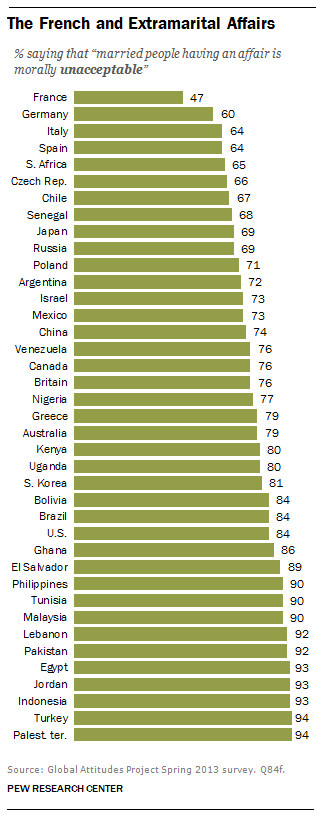
\includegraphics[width=0.95\linewidth]{images/Libro-img016.jpg}
  \begin{minipage}{\linewidth}
    \caption{Paesi dove l'infedeltà è più accettata}
  \end{minipage}
\end{wrapfigure}

Il fenomeno è stato ben analizzato da Roberto Lorenzini nella rubrica “Monogamia e tradimenti” apparsa su
stateofmind.it\endnote{\protect\url{https://www.stateofmind.it/category/rubriche/monogamia-e-tradimenti/} }. Secondo un analisi di
Gleeden.com, sito dedicato a donne in cerca di incontri extraconiugali, in Italia il 30\% resta sempre fedele per tutta
la durata della relazione, nel 40\% dei casi uno dei due partner tradisce, mentre, nel restante 30\% entrambi
tradiscono. Quindi, nel 70\% delle coppie c'è almeno un tradimento. Le percentuali concordano con
quanto raccolto su base europea dall'IFOP (istituto francese di opinione pubblica), mostrandoci
però più inclini al tradimento rispetto al resto d'Europa: il 45\% degli italiani ha dichiarato di
aver tradito il partner almeno una volta contro il 43\% della Francia, il 39\% della Spagna e il 36\% della Gran
Bretagna. Di cui solo un 27\% di italiani si è pentito mentre in Francia e Germania 28\%, Spagna 36\% e Gran Bretagna
50\%. 

Secondo una ricerca mondiale condotta da Pew
Research\endnote{\protect\url{https://www.pewresearch.org/fact-tank/2014/01/14/french-more-accepting-of-infidelity-than-people-in-other-countries/}
} il nostro paese appare molto più laico di quello che si pensa, infatti solo il 64\% degli italiani pensa che
l'infedeltà sia moralmente inaccettabile, piazzandosi al terzo posto dietro a Germania 60\% e
Francia 47\%, contro l'84\% degli USA e il 76\% dei Britannici. Sempre l'IFOP
ci riporta che, nonostante l'Italia sia la patria del cattolicesimo, per il 56\% degli italiani si
può essere innamorati del proprio partner e comunque tradirlo e, per il 63\% si può essere innamorati di due persone
contemporaneamente. Il 21\% degli intervistati ha una stabile e duratura relazione con l'amante,
mentre il 41\% ha avventure occasionali. Il 43\% degli infedeli si aspetta di essere perdonato e in effetti le
statistiche ci dicono che questo accade nel nel 70\% dei casi. Il 76\% degli Italiani dichiarato che rimanere fedeli è
possibile, contradditoriamente a quanto invece la realtà riporta nei fatti. Come tradimento viene considerato: baciare
alla francese (77\%), avere rapporti orali/sessuali (89\%), che raggiunge il 92\% se la pratica è regolare. 
\newline
\newline

\begin{figure}[H]
  \centering
  \begin{tikzpicture}
    \begin{axis}[
      ybar,
      xlabel={Categoria},
      ylabel={Valore},
      xtick=data,
      symbolic x coords={1, 2 - 3, 3 - 9, 9 - 25}, % Definizione delle categorie sull'asse x
      ]
      \addplot coordinates {(1,27) (2 - 3,36) (3 - 9,58) (9 - 25,49)}; % Primo set di valori
      \addplot coordinates {(1,21) (2 - 3,11) (3 - 9,46) (9 - 25,36)}; % Secondo set di valori
      \legend{Maschi, Femmine} % Legenda per i set di valori
    \end{axis}
  \end{tikzpicture}
  \caption{Sondaggio IPSOS che mostra la percentuale di tradimento (y) nei vari anni di matrimonio (x) in Italia. Tra il secondo e il terzo anno di matrimonio, la disparità tra maschi e femmine aumenta perché in quegli anni generalmente nasce il primo figlio; situazione che viene vissuta in maniera opposta dai due sessi, in quanto spesso accade che la donna impegnata nel nuovo ruolo di madre, trascurando il marito. O così dicono i mariti...}
\end{figure}

La credenza che gli uomini tradiscono per motivi sessuali mentre le donne per motivi sentimentali e per relazioni più
profonde, non sono più attuali. Le differenze ormai riguardano il singolo individuo e non più il genere. Tutti questi
dati si basano su interviste, dove è quindi possibile mentire, dati più oggettivi riguardano il test del DNA. In Italia
l'avvocato Gian Ettore Gassani presidente dell'associazione dei
matrimonialisti italiani riporta che: Secondo le stime ricavabili dai dati statistici, il 15\% dei secondi figli è di
un padre diverso da quello ufficiale e la percentuale arriva al 25\% nel caso dei terzi figli.

Detto questo, tornando allo spoiler iniziale, non c'è una vera regola, infatti, troviamo tante
tribù, come quella in degli zo'é in Amazzonia che sono poligami sia gli uomini che le donne. Nella
società zo'é tutti sono eguali, e per tradizione non esistono leader. Ma anche in Italia, se
guardiamo al passato, nell'impero romano non esisteva il matrimonio monogamico come lo intendiamo noi, l'uomo poteva
frequentare più di un amante pur avendo una moglie. È con l'avvento del cristianesimo e delle
proprietà private da tramandare in eredità che questo comportamento è iniziato ad essere punito. In linea di massima
essere una coppia aperta non rappresenta un problema di per sé in quanto non stiamo facendo nulla contro il nostro
partner, ma stiamo facendo altro con un'altra persona. Se usciamo con un amico o andiamo a letto
con un amante la quotidianità del nostro partner non cambia. Un mantra che abbiamo ripetuto spesso in questo libro è:
se non nuoce alla libertà altrui, allora tutto è consentito. La linea qua diventa sottile perché apparentemente il
tradimento sembra consentito ma, lo è solo se la coppia ha affrontato e accettato di essere una coppia aperta,
altrimenti la libertà del partner è minata in maniera nascosta. Infatti, se culturalmente l'idea
della coppia prevede di non tradirsi e non comunico al mio partner che per me invece l'idea di
coppia è diversa dalla sua, lui o lei si impegnerà a non tradirmi, convinto che lo faremo anche noi, quindi,
implicitamente, lui o lei si precluderà la possibilità e la libertà di avere altri partner.

In questo periodo storico viviamo l'ipocrisia di una società che da una parte promuove la
sessualità senza tabù e incoraggia le persone a fare più sesso con più persone possibili,
dall'altra ci mortifica e ci fa vergognare del tradimento, anche solo il pensare che una persona
possa essere attraente è già tradimento per qualcuno. Crediamo che se siamo attratti dal/la collega appena assunto/a
dobbiamo trovare delle giustificazioni per non cadere nell'erroneo pensiero che, se ho voglia di
un'altra persona allora c'è qualcosa che non va nel mio rapporto. Come
abbiamo scritto precedentemente, citando Schopenhauer, oscilliamo tra la noia e il dolore. La nostra specie ci ha
fornito la noia per portarci all'insoddisfazione così da superare i nostri limiti. Possiamo
credere che se fossimo fidanzati con Uma Thurman, Victoria Beckham, Siena Miller, Jennifer Garner o Jarry Hall, non ci
stuferemmo mai, ma questo solo perché non ci state assieme, infatti, tutte queste donne sono state tradite.

\begin{mdframed}[linewidth=1pt]
A chi piacciono le donne magre e gli uomini muscolosi?

Secondo uno studio dell'Università di Saint Andrews, in Scozia sono in pochi ad apprezzare queste caratteristiche. Con
un campione di 146 uomini e donne eterosessuali di età compresa tra i 18 e 31 anni è stato chiesta ai partecipanti di
guardare delle immagini e scegliere quelle che preferivano come fisico ideale per se stessi e per il loro partner per
una relazione breve e quello per una relazione lunga. Gli uomini hanno sopravvalutato l'aspetto muscoloso nelle
preferenze delle donne, e le donne hanno sopravvalutato la magrezza nel corpo femminile. Inoltre, le percezioni errate
erano più marcate quando si pensava a relazioni più brevi.
\end{mdframed}

Paradossalmente, chi ha una buona vita sessuale di coppia, può essere più propenso al tradimento. Proprio tale
soddisfazione sessuale provoca una crescita dell'autostima che potrebbe accrescere il desiderio
verso persone al di fuori della coppia. L'appetito vien mangiando quindi secondo questa ricerca
della Florida State University pubblicata nel 2018 dalla rivista scientifica Journal of personality and social
psychology. Altre volte invece succede l'opposto. Siccome non ci si sente meritevoli di amore,
inconsciamente si cerca un'avventura, anche dando poca attenzione al non essere scoperti, proprio
per distruggere quella relazione e giustificare quello che si pensava. La profezia che si auto avvera.

Non possiamo quindi decidere di essere o non essere attratti da una persona, possiamo però, scegliere di non farlo
diventare un problema. Siccome capita a tutti, non può essere un problema e non ha senso tormentarsi di sensi di colpa
se ci sentiamo attratti da qualcuna/o.

Nel racconto biblico dell'adultera, quando le persone stanno per lapidarla, Gesù dice: Chi è senza peccato scagli la
prima pietra. Pian piano i presenti iniziarono a far cadere le pietre a terra e, i primi furono i più anziani e per
ultimi i giovani. Questo perché gli anziani, con più esperienza, riconoscono le contraddizioni
dell'essere umano e sanno, che anche loro, in una certa situazione, avrebbero potuto compiere
questo gesto sbagliato. L'atto del perdono, è un atto di riconoscimento verso se stessi e delle proprie contraddizioni.

Quindi come se ne esce? Con la cara vecchia consapevolezza. Dobbiamo vedere le cose per ciò che sono, un infatuazione è
un infatuazione, non ha altri messaggi nascosti, inconsci, non significa ne che la nostra relazione stia andando male,
ne che lei/lui sia giusta/o per noi. Secondo Esther Perel in Così fan
tutti\endnote{\protect\url{https://www.amazon.it/dp/B07CT6NRQ5/} }, quando un matrimonio finisce per iniziare una nuova storia con
l'amante, questa nuova coppia statisticamente ha poche probabilità di durare. Sembra strano, in
quanto si è messo a rischio così tanto con un divorzio e tutto ciò che ne consegue. Ma quando subentra la quotidianità
del “porta fuori la spazzatura” e “abbassa la tavoletta” la magia è destinata a svanire. Il problema non è quindi la
quotidianità che è inevitabile, normale e succede a tutti, ma etichettare la quotidianità alla banalità, alla noia, al
problema a qualcosa di sbagliato che non dovrebbe esistere in una coppia
innamorata\endnote{\protect\url{https://www.stateofmind.it/2021/01/tradimento-relazioni-sentimentali/} }.

la Psicologia dell'adulterio è falsata dalla morale convenzionale che nei paesi monogami,
l'attrazione per una persona non possa coesistere con il serio affetto per
un'altra. Tutto questo è falso - \ Bertrand Russell (Matrimonio e
morale\endnote{\protect\url{https://www.amazon.it/dp/B08ZNR576M} })

Molte volte il disagio che sentiamo non è tanto per via dall'attrazione che sentiamo per
un'altra persona, ma il sentirsi sbagliati, diversi, da quello che culturalmente viene ritenuta la
norma, ovvero la monogamia in questo caso, ma il discorso può essere esteso a tutti i disagi molto spesso. Oltre a
questo, bisogna comunque fare una scelta e, come spesso accade, ogni scelta comporta una rinuncia. Da una parte
chiudere la relazione principale con tutto ciò che ne comporta, divorzi, figli, casa ecc…
dall'altra parte rinunciare all'altra relazione con la perdita
dell'effetto vivificante e dell'arricchimento che comportava. Come abbiamo
visto ogni relazione d'amore, superata la fase iniziale di innamoramento, è finalizzata al
mantenimento dell'identità e alla realizzazione di progetti nel tempo coerenti con i propri valori
di coppia, come ad esempio l'avere dei figli. In conclusione, secondo Roberto Lorenzini partner
secondari e transitori, potrebbero anche arricchire la coppia. Il conflitto che eventualmente potrebbe nascere,
durerebbe soltanto per la fase dell'innamoramento (corrisposto). Quindi la monogamia che viene
continuamente smentita nella pratica porterebbe più sofferenze e rinunce, che vantaggi costringendo alla segretezza e
all'inganno, vera devastante insidia per la coppia principale. 

Per concludere non so cosa sia meglio, forse dipende da persona a persona, ci sono pro e contro in entrambe le scelte,
quello che importa è che entrambi siano d'accordo e consapevoli della propria scelta. Qualsiasi
cosa decidiamo essere giusta per noi, non deve essere un modo per fuggirsi. Ad esempio per qualcuno il poliamore
potrebbe essere un modo per non impegnarsi, per altri potrebbe essere la soluzione e, la fine di ogni desiderio, ma
come abbiamo visto, una persona con questa idea, se dovesse riuscire a costruire una situazione simile, probabilmente
quando avrà tre partner ne desidererà un quarto, poi un quinto e così via all'infinito.

\begin{mdframed}[linewidth=1pt]
Appuntamenti online

Anche questa è un opzione percorribile e valida oggi giorno, ma con moderazione. Secondo gli psicologi dell'università
olandese di Tilburg, più profili si guardano, più aumenta la tendenza a chiudersi e sviluppare una mentalità di
rifiuto. Questo dipende dall'enorme mole di opzioni disponibili, che può accrescere i sentimenti
di insoddisfazione e pessimismo nella ricerca di un partner. Più tempo si passava a guardare profili e più cresceva il
pessimismo sull'essere accettati loro stessi, che a sua volta era collegato alla tendenza al rifiuto.
\end{mdframed}

\subsection{Può durare? E come?}
Secondo Massimo Recalcati un amore dura quando un corpo sa rivelarsi sempre nuovo, come un libro o una canzone che,
anche dopo anni, non via ha ancora stufato. Un'altra caratteristica, contraria
all'amore romantico della televisione che ci ha imposto un immaginario romantico irrealizzabile è
la solitudine. È importante ritagliarsi dei momenti di solitudine rimanere due individui distinti, con le proprie
personalità, riuscendo a non fondersi in un unico piatto elemento. Una coppia esiste non per fondersi, o per avere
interessi comuni. ma perché ognuno realizzi la propria natura. Anzi, a volte avere interessi comuni potrebbe essere uno
svantaggio, perché si avrebbe meno tempo per stare da soli, cosa controintuitiva ma necessaria. Questo comporta che ci
saranno delle differenze tra i due partner e, alcune di queste potrebbero essere etichettate come difetti.
L'errore è aspettarsi il principe azzurro o l'equivalente femminile,
perfetto, senza difetti, perché questo ci porterà ad imporci di voler cambiare l'altro. Molto
spesso capita di allontanarsi dal partner perché “è cambiato” ma in realtà è molto difficile anche diventare
qualcos'altro, è più probabile che il nostro partner fosse sempre stato così, solo che non
volevamo vederlo, perché ci siamo innamorati dell'innamoramento invece che della persona. Se
chiedessimo a una persona, cosa ti piace del tuo partner? E lei rispondesse: mi porta fuori a mangiare, mi compra i
fiori, mi dice cose carine ecc... Noteremmo che non ci ha detto nulla di cosa le piace di lui, ma solo cosa lui fa per
lei. Come abbiamo visto, quando cerchiamo di cambiare l'altro, spesso otteniamo
l'effetto paradossale di ottenere l'esatto contrario, ad esempio, una persona
fedele potrebbe diventare un traditore. In amore o ti fidi o non ti fidi. Scovare un tradimento è più difficile di
quanto si pensi, così, se cerchi prove che confermino un sospetto, troverai cose neutre ma che dal tuo punto di vista
saranno invece sospette, portando anche un innocente ad apparire come un traditore. Una buona relazione non ti limita,
non ci sono giochi di potere, ricatti, se mi ami allora ecc... O ad esempio, dare al partner tutto ciò che vorremmo che
ci desse in modo da pretendere che anche quest'ultimo ricambi e, facendolo sentire in colpa
qualora non soddisfasse le nostre tacite richieste. Ignorando che che magari anche il nostro partner sta dando alla
relazione quello che lui vorrebbe ricevere, in quanto crede che possa far piacere, anche se non in linea con quanto
aspettato dall'altra parte, generando così un senso di inadeguatezza nonostante questo impegno mal
orientato, causa della cattiva o assente comunicazione.

Ancora una volta torna il discorso di conoscere se stessi, perché ovviamente non dobbiamo voler accettare tutto
dell'altro. Dobbiamo capire cos'è importante per noi, quali sono i nostri
valori e, se il nostro partner è in linea con questi, dovremmo imparare ad apprezzare o, quantomeno accettare i suoi
difetti. Di conseguenza il litigare non diventa un campanello d'allarme che segnala un problema
nella coppia, ma è la naturale dinamica di qualsiasi tipo di relazione che dura nel tempo. Anzi, al contrario se si
litiga poco potrebbe celarsi un'eccessiva accondiscendenza da parte di uno dei due partner. Il
problema è quando si litiga troppo e male, questo logora il rapporto.

Secondo uno studio della Northwestern University un buon esercizio che permette di allenarci a vedere i motivi del
disaccordo dura solo sette minuti per tre volte all'anno. Bisogna scrivere del più recente
conflitto avuto con il partner assumendo il punto di vista di un'ipotetica terza persona che desidera il bene di
entrambi. Le coppie che hanno svolto questo esercizio non litigavano meno delle altre, ma tornavano più facilmente ad
uno stato di serenità.

Anche nelle relazioni si tende all'omeostasi, ovvero, quella tendenza naturale di mantenere una
certa stabilità sia chimica interna che comportamentale. Quindi si preferiranno tipologie di persone e di relazioni che
li confermeranno le nostre aspettative, su noi, gli altri e le relazioni. Preferiamo rimanere in relazioni non
soddisfacenti piuttosto che smentire le nostre credenze, anche su quello che proviamo, portando alla famosa profezia
che si autorealizza. Ad esempio: un individuo che si ritiene vulnerabile, per via delle sue esperienze passate nei
momenti di difficoltà, in un momento di stress, potrebbe porsi con rabbia, suscitando nel suo interlocutore un normale
distanziamento, freddezza, o abbandono, confermando così l'idea che aveva di sé stesso. Le
ricerche sostengono che impariamo principalmente dalla nostra famiglia la regolazione emotiva e come stare in coppia.
Capita spesso di dire che incontriamo sempre le persone sbagliate, non rendendoci conto che forse siamo noi a indurre
questi comportamenti
nell'altro\endnote{\protect\url{https://www.stateofmind.it/2020/06/attaccamento-disregolazione-emotiva/}.} Non
chiediamoci cosa il partner dovrebbe fare per noi, ma cosa noi possiamo fare per lui. A volte abbiamo delle aspettative
tali che nessun essere umano sulla terra riuscirebbe a soddisfarle. La cultura ci ha abituato che se è vero amore,
tutto viene da se, ma la realtà è che le relazioni, come tutto nella vita, richiedono impegno. Non cercare la persona
giusta, ma diventa tu la persona giusta. Ascoltando i suoi bisogni, non colpendolo nei suoi punti più deboli, ma
sostenendolo e incoraggiandolo sempre.

\begin{mdframed}[linewidth=1pt]
Qual è la durata ideale di ua rapporto sessuale?

10 minuti secondo un'indagine della Society for Sex Therapy and Research di Washington. Lo studio ha individuato nella
fascia 7-13 minuti la perfetta durata per fare l'amore. Oltre i 13 minuti, distrazioni, stanchezza e noia tendono a far
calare il desiderio, mentre sotto i 7 minuti è probabile che almeno uno dei due partner resti insoddisfatto.
\end{mdframed}

Ancora una volta portiamo quindi l'attenzione sulle cose positive, anche quando non siamo con il
nostro partner, pensiamo a quanto ci da invece di portare l'attenzione sulle sue mancanze e sui
suoi difetti. 

Come si fa a far durare una relazione? Alcuni ricercatori hanno programmato un'intelligenza
artificiale per rispondere a questa domanda e ha trovato questi
ingredienti\endnote{\protect\url{https://www.pnas.org/content/early/2020/07/21/1917036117} }
\endnote{\protect\url{https://www.wired.it/scienza/lab/2020/07/28/intelligenza-artificiale-relazioni-consigli/} }:

\begin{enumerate}
\item Impegno del partner percepito (ad esempio sentire che anche il partner si stia impegnando affinché la relazione
duri per sempre)
\item Gratificazione (sentirsi fortunati ad avere quella persona a fianco), 
\item Soddisfazione sessuale
\item Appagamento del partner (credere che la relazione renda felice il proprio partner) 
\item Conflitti (quanto spesso si litiga)
\end{enumerate}
E quali sono invece i motivi più frequenti che possono portare alla rottura di una coppia?
\endnote{\protect\url{https://www.stateofmind.it/2021/07/relazioni-sentimentali-durature/} \ }

\begin{enumerate}
\item Soldi: un partner disapprova le spese dell'altro\newline
Possibile soluzione: si può discutere a stabilire un budget per le spese personali o extra
\item Sesso: ci si accusa di essere troppo pigri o inibiti \newline
Suggerimento: comunicazione
\item Gelosia\newline
Soluzione: forse nessuna, senza fiducia nessuna comunicazione può funzionare
\item Tempo libero: dove andiamo, film, serie TV, spesso nascondono un modo per stabilire chi comanda \newline
Suggerimento: fare un po' per uno trovando il bello nelle scelte altrui
\item Parenti \newline
Suggerimento: cercare di frenare i genitori
\item Figli
\item Amici del partner \newline
Suggerimento: tolleranza
\item Casa e faccende domestiche \newline
Suggerimento: fare una tabella delle mansioni
\item Animali domestici
\end{enumerate}
Come spesso si legge, effettivamente, uno degli strumenti per riuscire a mantenere un buon rapporto è la comunicazione,
che non significa parlare tanto. Come scritto in L'arte di non amareggiarsi la
vita\endnote{\protect\url{https://www.amazon.it/dp/B00B0ZN91G} }, un giorno alla settimana compilare la "Lista
di suggerimenti con amore" e consegnarla al proprio compagno. Questa lista conterrà tutto ciò che
vorremmo cambiare del nostro partner. La peculiarità di questa lista è che ogni suggerimento va concluso con questa
frase: "…ma se non lo farai, ti amerò ugualmente per il resto dei miei
giorni". 

Anche il legame sessuale con il tempo tende ad affievolirsi. Alcuni
studi\endnote{\protect\url{https://www.researchgate.net/publication/280870836\_Does\_Sexual\_Satisfaction\_Change\_With\_Relationship\_Duration}
} dimostrano infatti che la soddisfazione sessuale all'interno di una relazione raggiunge il picco
dopo 12 mesi. Un'altra
ricerca\endnote{\protect\url{https://www.vice.com/en/article/a3bnez/women-get-bored-in-bed-faster-than-men} } ha rilevato che le
donne sono più propense ad annoiarsi nel fare sesso sempre con lo stesso partner rispetto agli uomini. Secondo i
ricercatori la casa diventa il luogo associato al relax, quindi un modo per mantenere vivo il legame sessuale è cercare
di provare cose nuove e parlare dei propri
desideri\endnote{\protect\url{https://www.vice.com/it/article/5d3pm3/sesso-noioso-fidanzato} }. La sessuologa Emily Nagoski
consiglia di ritagliarsi uno spazio, volontariamente, dove ci si mette a letto, sentendo il contatto della pelle del
partner, per creare l'atmosfera e far nascere il
desiderio\endnote{\protect\url{https://www.ted.com/talks/emily\_nagoski\_how\_couples\_can\_sustain\_a\_strong\_sexual\_connection\_for\_a\_lifetime}
}.

Se si ha meno voglia di fare sesso, non significa che le cose stiano andando male. Stando spesso assieme è normale che
il desiderio si affievolisca. Inoltre, come spiega Yuri Ohlrichs, capita di associare al sesso nelle relazioni a lungo
termine all'avere dei figli, e magari, in questo momento non ne senti il bisogno. Anche qua
percepiamo più il problema in relazione agli altri e a ciò che riteniamo dovrebbe esserci piuttosto che della questione
in sé. Non tutte le relazioni sono uguali e con i medesimi bisogni o che le vostre serate sul divano debbano per questo
sembrarvi meno preziose rispetto a coppie con una vita sessuale più
attiva\endnote{\protect\url{https://www.vice.com/it/article/xgdv4z/calo-desiderio-sessuale-in-coppia} }.

\begin{mdframed}[linewidth=1pt]
Possono essere utili le pause di riflessione e i tira e molla?

No secondo un team di studiosi delle università del Missouri e dell'Ilinois. Analizzando un campione di 545 persone
hanno notato più alti livelli di ansia e depressione che alla lunga portano al deterioramento del rapporto. I motivi
che hanno portato all'allontanamento di uno dei due partner restano anche dopo la chiusura del
rapporto. Se si prende una pausa dove si analizza onestamente anche le proprie mancanze ci sono più possibilità di
risanare il rapporto, ma difficilmente si riesce a cambiare qualcosa, specialmente nel breve termine. 
\end{mdframed}

Ne il segreto dell'amore felice\endnote{\protect\url{https://www.amazon.it/dp/B00GH162G2/} } di Raffaele Morelli ho trovato dei
pensieri che si fondano sul non farsi domande riguardo i temi dell'amore, liberarsi dai giudizi e
vivere le esperienze per come sono. Non chiedersi se siamo innamorati, non dirlo agli altri per non far sfumare quello
che proviamo. Se analizziamo e riempiamo di giudizi i nostri sentimenti, finiamo per distruggerli. Non sforziamoci di
farlo durare se vogliamo che duri. I rapporti di coppia non vanno migliorati, perché ne farebbe perdere la spontaneità.
Non pretendere di innamorarti “come una volta”. Non esiste amore con la “a” maiuscola o minuscola. Abbiamo una lista
delle caratteristiche che deve avere l'amore per essere con la “a” maiuscola:
l'età, interessi, hobby, aspirazioni, status, se vuole figli ecc…. Ma così invece di un sogno,
diventa una gabbia, perché se, quando incontriamo qualcuno, controlliamo la nostro lista e, se manca qualcosa allora
dobbiamo soffrire o lasciare perdere questa persona impedendoci questa esperienza.

Oltre a questo ho trovato un pensiero che riporta tutto dentro di noi e non sugli altri, sia nel bene che nel male.
L'altro attiva delle parti che sono già presenti in noi. 

"Nessuna cultura del passato ha mai distinto tra sesso e amore, bollando il primo come sbagliato ed
esaltando il secondo. Io sostengo proprio il contrario: che di fronte a Eros “dobbiamo” essere soli, in quanto in
realtà stiamo facendo l'amore con il dio stesso. La partita si gioca tra noi e lui, il partner è
solo un'occasione che ci è capitata." 

Anche quando ci arrabbiamo, siamo portati a pensare che sia colpa dell'altro, ma quella parte era
già dentro di noi, volevamo già manifestarla, abbiamo solo trovato il pretesto giusto in base ai significati che
abbiamo dato del mondo. Alcune persone lamentano di non riuscire a trovare storie serie, perché nessuno vuole più
impegnarsi, ma più probabilmente sono proprio loro a cercare questo tipo di relazioni, che però, essendo culturalmente
malviste e, non volendo essere giudicate negativamente, si trovano con una parte di loro che comunque andrà a
soddisfare i loro bisogni e, un'altra, che per giustificarsi, modificherà questa narrazione
attribuendo le “colpe” all'esterno. Crediamo di innamorarci di una persona sposata in modo
casuale, quando invece è l'inconscio a sceglierla per qualche motivo. Forse perché abbiamo paura
della convivenza e, in questo modo ci garantiamo di non dover affrontare questo cambiamento, forse perché così ci
sentiamo più liberi, o forse per mille altri motivi.

Le persone che incontriamo sono la scintilla. Per questo i giudizi, anche sulla fedeltà, diventa no un freno per parti
già presenti dentro di noi. Quando senti di innamorarti di un'altra persona, la tua mente non ti sta chiedendo di
scegliere tra le due persone. Ti sta solo mostrando che c'è un lato di te che vuole emergere e, per farlo, come succede
per ogni lato di noi, lo fa attraverso l'eros. Ti stai innamorando di te attraverso di
lei/lui\endnote{\protect\url{https://youtu.be/lPRLiwrUrNA} \ }. 

Morelli nel suo libro parla anche di alcune storie. Una paziente racconta che da due anni ha una relazione molto
importante con un uomo più grande, sposato e con due figli e questa cosa la fa soffrire. Se una relazione diventa
dolorosa è perché abbiamo introdotto le nostre definizioni, i nostri progetti di vita. Possiamo solo goderci le cose
così per come ci capitano, altrimenti le trasformiamo in un inferno di aspettative che quasi mai si avverano. Una tua
parte si è innamorata proprio di questa situazione, forse non vuole che si trasformi in un matrimonio, non possiamo
sapere i suoi piani, possiamo viverla per come è. Non esistono scelte sbagliate per la nostra crescita. Noi facciamo le
scelte che facciamo perché in quel momento, per la nostra maturità avevamo bisogno proprio di questo. 

\begin{mdframed}[linewidth=1pt]
Secondo uno studio della Northwestern University (Usa) un esercizio per mantenere alta la soddisfazione della coppia è
scrivere su un foglio di carta circa il conflitto più recente con il partner assumendo il punto di vista di
un'ipotetica terza persona che desidera il bene di entrambi. Per diminuire gli scontri basterebbe impegnarsi soltanto
tre volte all'anno per sette
minuti\endnote{\protect\url{https://www.focus.it/comportamento/psicologia/come-non-litigare-con-partner-salvare-crisi-coppia} }.
\end{mdframed}

\subsection{Comunicazione}
Uno dei libri sul tema che ho apprezzato di più è stato proprio il famoso: Gli uomini vengono da Marte le donne da
Venere\endnote{\protect\url{https://www.amazon.it/dp/B00AA6F2OI/ref=dp-kindle-redirect?\_encoding=UTF8\&btkr=1} }. Essendoci delle
differenze comportamentali tra uomini e donne, che però non si conoscono, tendiamo ad avere aspettative sbagliate.
Pensiamo che se il nostro partner non si comporta come faremmo noi, c'è un problema. 

PARLARE DELLE PRIME PAGINE CON DIFFERENZE TRA UOMINI E DONNE. GLI UOMINI RISOLVONO PROBLEMI E VANNO NELLA CAVERNA, LE
DONNE CERCANO SOLUZIONI PARLANDO CON LE ALTRE E VANNO NEL POZZO.

Dare un consiglio a una donna è segno d'interesse. Per una donna, se una cosa funziona, può
funzionare ancora meglio. Mentre gli uomini, orientati alla soluzione, non cambiano qualcosa che funziona. infatti gli
uomini reagiscono male ad ogni tentativo di correggerli o di cambiarli. Ogni consiglio non richiesto viene percepito da
un uomo come mancanza di fiducia e competenza nelle sue capacità. Come se fosse rotto e andasse aggiustato. Quando una
donna, invece, esterna i suoi sentimenti, l'uomo pensa che sia in cerca di soluzioni più che di
comprensione. Così la donna sente sminuire i suoi problemi, perché percepisce che secondo l'uomo
si possano risolvere con un paio di consigli che gli sono venuti in mente in quel momento. In questo modo
l'uomo sa comunicare disponibilità. Così, una frase detta da una dona tipo “Non usciamo mai” viene
percepita dall'uomo come la richiesta di una soluzione al suo cruccio. Così risponde “non è vero
siamo uscititi settimana scorsa” di conseguenza lei la percepisce come un tentativo di sminuire i suoi sentimenti e di
liquidarla con una risposta facile. Quando un uomo vede che il suo consiglio e la sua disponibilità non sono stati
apprezzati, troverà difficile continuare ad ascoltare la sua compagna, perché non si sente utile, cosa per lui
importante, ignorando che che per una donna, già il parlare dei propri problemi equivale a sollecitare una soluzione.
Quando gli uomini diventano consapevoli di questo aspetto, si sentono sollevati nel sapere che non è una loro
responsabilità risolvere i problemi delle loro compagne. Gli uomini quando parlano tendono a scambiare informazioni,
mentre le donne emozioni. Si stima \ infatti che, probabilmente anche per questa ragione, le donne usano in media 8
mila parole al giorno contro le 4 mila degli uomini. Quando un uomo è dentro la sua caverna e la donna se ne accorge,
siccome lei non reagirebbe in questo modo, mostra il suo interesse domandando se va tutto bene. In questo modo,
inconsapevolmente, sta bloccando un momento di introspezione a cui l'uomo rispenderà con un “va
tutto bene”. Gli uomini solitamente tendono a chiudersi nel silenzio piuttosto che esternare un disagio e spiegare di
aver bisogno solo di un po' di tempo per restare da soli. Una donna però percepisce questo silenzio, erroneamente, come
un “non voglio parlare con te”. Uomini e donne fisiologicamente vivono dei fasi cicliche. A volte gli uomini tendono ad
allontanarsi, per poi riavvicinarsi, magari proprio nel momento in cui la donna cerca maggiore intimità. Allo stesso
modo anche le donne ciclicamente sentono un vuoto, dove cercano amore, attenzioni e sostegno per riempirlo, per poi
tornare nuovamente piene di energia e con molto da offrire.Sforzarsi costantemente di essere allegri e affettuosi può
portarvi a sopprimere le vostre emozioni negative. Nel tempo, questa pratica può portare alla riduzione della vostra
capacità di provare emozioni in generale. Tuttavia, ci sono situazioni in cui è appropriato sentire e mostrare
tristezza ed empatia. Ad esempio, quando un amico vi parla della morte di una persona cara, è importante mostrare
compassione e offrire supporto. D'altro canto, è anche importante trovare un equilibrio tra il riconoscimento delle
proprie emozioni e il non lasciare che la rabbia e la tristezza prendano il sopravvento. Non dovreste cercare di essere
costantemente felici, poiché questo può portare a sentimenti di colpa e frustrazione quando non ci si sente così. È
importante utilizzare strategie, come la rivalutazione dei pensieri, per accettare le emozioni negative e coltivare la
speranza che le cose possano migliorare. La chiave è trovare un equilibrio personale nella gestione delle emozioni,
riconoscendo la loro importanza e permettendo loro di essere parte della nostra esperienza
umana\endnote{\protect\url{https://www.ted.com/talks/ted\_ed\_how\_to\_manage\_your\_emotions?language=it} }. Quando uno dei due
partner è troppo presente, per l'altro potrebbe diventare faticoso il vedersi, rispondere al
telefono così frequentemente e senza accorgersi, si preferisce mettere distanza. Altre volte succede, più per
l'uomo e la sua necessità di risolvere i problemi, che se trovandosi una donna poco indipendente,
con poche amicizie o che comunque ha difficoltà ad organizzarsi cose per conto suo, lui senta la responsabilità di
dover provvedere a tutto, portando disagi sul lungo periodo. Al contrario, persone troppo aggressive o autonome
lanciano il messaggio: io non ho bisogno di te. In questi casi il partner che percepisce questa distanza e, che ha
contribuito seppur inconsciamente a creare, potrebbe aggravare la situazione accusando il compagno o la compagna di
immaturità e, portandolo/a in alcuni casi a sentirsi come il problema, quando magari invece è stata una reazione
comprensibile. Quando la discussione inizia a far leva sui sensi di colpa, non è ovviamente detto che chi lo fa abbia
ragione, ma quando si è coinvolti direttamente è difficile osservare la questione con lucidità e si può arrivare anche
a credere che il partner abbia ragione e che siamo noi ad essere il problema, passando da vittima a carnefice.

Insomma, con modalità diverse, ma tutti cerchiamo amore, quando le cose in una coppia non funzionano è perché non ci
sentiamo amati, non lo percepiamo in base a quello che noi definiamo come segnali d'amore. Durante
i litigi un uomo dovrebbe porre più domande, dimostrando interesse e di comprendere quello che è il suo mondo
interiore. Meglio chiedere, secondo te cosa dovremmo fare? Rispetto a, dovresti fare così! Questo amplificherebbe
quello che lei emotivamente ha già ingigantito. Mentre una donna dovrebbe parlare meno dei sui sentimenti.

DOPO PAGINA 162 CI SONO (PENSO) I CONSIGLI PER LEI, PER EVITARE DI LITIGARE

A PAGINE 222 UN DIALOGO TIPO MARZIANO E VENUSIANO

Ma perché uomini e donne sono così diversi? Lo psicologo John Gottman, uno dei più grandi studiosi della relazione di
coppia, ha tentato di dare una spiegazione in Intelligenza emotiva per la
coppia\endnote{\protect\url{https://www.amazon.it/dp/B00G6KL9DU} }. Le donne in fase di allattamento possono produrre più o meno
latte in base allo stress, perciò la selezione natural ha premiato gli individui che riuscivano velocemente a
rilassarsi. Per gli uomini invece, in quanto cacciatori, mantenere alta la vigilanza e
l'adrenalina era fondamentale per la loro sopravvivenza. Studiando i litigi John Gottman ha notato
che gli uomini tendono di più a elaborare pensieri negativi in modo da mantenere alto lo stress, mentre le donne si
rifugiano in pensieri più lenitivi che le aiutano a calmarsi e a cercare una conciliazione.\newline
Per questo motivo gli uomini tendono ad andare di più sulla difensiva durante un conflitto, in maniera vittimistica,
bellicosa o silenziosa.

Un altro tema frequente è quello che vede il nostro partner coinvolto in una disputa: se non condividiamo il suo punto
di vista dobbiamo dirglielo o dobbiamo sostenerlo? Entrambe le cose secondo John Gottman, ma con i giusti momenti.
Inizialmente il nostro partner si rivolgerà a noi per cercare aiuto emotivo e non per un consiglio, quindi lo
sosterremo. Quando la carica emotiva sarà passata, allora potremmo, in punta di piedi, provare a fargli vedere il
nostro punto di vista. La base per affrontare i problemi è sempre la stessa: Comunicare accettazione della personalità
del nostro partner, comprendere i suoi bisogni e i nostri bisogni, e infine comunicarli trovando un compromesso.
L'accettazione è il primo passo fondamentale, se vi sentite giudicati, fraintesi o rifiutati, non
riuscirete a comprendere l'altro e andargli incontro. Le persone cambiano solo per pensano di
piacere agli altri e si sentono accettate per come sono. Se un vostro amico dimentica l'ombrello
in giro, semplicemente gli dite: “Hai dimenticato l'ombrello”, non ci salterebbe mai in mente di
dire: Ma che cos'hai? Non fai altro che dimenticare in giro gli oggetti. Per
l'amor del cielo, cerca di stare più attento! 

Il seguente esempio, tratto da Intelligenza emotiva per la coppia\endnote{\protect\url{https://www.amazon.it/dp/B00G6KL9DU} }, vede i
due partner fermi sul problema dell'ordine della casa. Lei vorrebbe che lui sia più ordinato,
mentre lui vuole dedicarsi alle sue cose nel tempo libero quando è a casa. Quali sono i desideri che stanno dietro
questa richiesta? Per lei un senso di ordine e, per lui, il bisogno di libertà a casa sua. Per trovare un compromesso
dobbiamo individuare le aree non negoziabili. Lei non può accettare i piatti e il bagno sporco, lui invece non vuole
rimettere in ordine le sue carte finito di lavorare, perché lo costringerebbe a riorganizzarle nuovamente il giorno
seguente. Fortunatamente le aree non negoziabili non sono in contrasto tra loro, così possiamo lavorare su delle aree
di flessibilità: Lei può vivere con un po' di disordine, a patto che il bagno e la cucina siano
puliti. Lui può lavare i piatti e il bagno a patto di non doverlo fare in continuazione. Lei non lo assillerà con la
mania dell'ordine più di una volta alla settimana, ma se lui non si comporterà come è stato
stabilito, lei raccoglierà tutto e glielo metterà sul pavimento del suo studio di casa. Lei odierà sempre il disordine
e, lui odierà sempre l'ordine, per questo entrambi dovranno stare attenti di continuo a rispettare
i patti. Stare assieme richiede un certo impegno, contrariamente a quello che la filmografia ci ha insegnato. Secondo
\ John Gottman le coppie che funzionano condividono 5 ore o più di qualità alla settimana con il proprio partner,
inoltre, non bisogna avere paura della discordia o di litigare, questo infatti non è sinonimo che il rapporto stia
andando in una direzione sbagliata. E non sempre il diverbio si risolve discutendo all'infinito.
Molti rapporti durano felicemente nascondendosi delle cose che fanno arrabbiare l'altro. Altri
ancora, quando litigano, chiudono la discussione, magari momentaneamente, o magari no e, ognuno si allontana per
dedicarsi ai propri hobby. Per qualcuno invece l'amore non è al primo posto spiega Ombretta
Cecchini\endnote{\protect\url{https://www.spreaker.com/user/dott.ssa\_ombrettacecchini/non-sei-la-sua-priorita} }. Una persona
potrebbe amare il volontariato e essere meno dedito verso il partner. Questo non significa essere egoisti, anaffettivi
o narcisisti. Non tutti sono uguali o hanno lo stesso modo di amare. Altri urlano e gridano, poi ad un certo punto uno
dei due tira fuori la lingua e fa il bambino per sciogliere la tensione, questo è quello che si chiama: tentativo di
riparazione. Spesso è controproducente affrontare un diverbio quando l'altro non ne ha alcuna
intenzione, magari è meglio aspettare un momento migliore, specie se l'altro sta facendo qualcosa
che gli piace. Insomma, la regola è che tante volte non c'è una regola, ogni coppia deve trovare
il suo modo, il suo equilibrio. 

In Quiet\endnote{\protect\url{https://www.amazon.it/dp/8845294064} } di Susan Cain viene riportato un esempio dove un marito,
rassettato la cucina, la mattina seguente sente urlare: “Questa cucina è un porcile!{\textquotedbl} Entrando e
guardandosi attorno, si possono notare al massimo tre o quattro bicchieri in giro. La foga di quei momenti per Jennifer
è del tutto naturale, è il suo modo di dire: Cavoli, mi piacerebbe che tenessi un po' più in ordine la cucina. Se me lo
comunicasse in questi termini le risponderei: Piacerebbe anche a me, amore, scusami se non l'ho fatto. Invece in questo
modo aggressivo verrebbe naturale rispondere con altrettanta violenza. Nel nostro esempio però, il marito ha
riconosciuto che questo è il modo in cui la moglie si esprime e che non è poi la fine del mondo.

Gary Chapman ne i cinque linguaggi dell'amore\endnote{\protect\url{https://www.amazon.it/dp/8801023723} } ha individuato cinque
modalità appunto che le persone ricercano nel proprio partner.

\begin{enumerate}
\item Parole di rassicurazione e apprezzamento: Se una moglie vuole che il marito imbianchi le pareti non deve porsi
pretendendolo in continuazione. Se lo si dice una volta lui lo sa, dirlo altre mille volte equivale a pretenderlo e
imporsi in modo autoritario e non equanime. Molto più efficace è invece comunicare apprezzamento per tutte le altre
cose buone che fa, come portare fuori la spazzatura.
\item Momenti speciali: Quando un coniuge critica il partner perché lavora troppo, o perché esce spesso con gli amici,
non sta dicendo che odia il suo lavoro, ma semplicemente vede in questo l'oggetto che sottrae a
lei o a lui il tempo che vorrebbe che venisse dedicato. Per queste persone, che ricercano momenti speciali da passare
assieme, anche il semplice parlare non lo si può fare guardando la televisione, ma dedicando i giusti momenti di una
condivisione sincera.
\item Ricevere Doni: Non devono essere per forza dei doni costosi, anche in questo caso è il pensiero quello che conta.
\item Gesti di servizio: Fare qualcosa per l'altro come pulire, lavare, tagliare l'erba eccetera.
\item Bisogni fisici: Come ricercare carezze, abbracci o sesso ad esempio. 
\end{enumerate}
Come possiamo capire con quale linguaggio vorremmo che il nostro partner utilizzasse con noi? E quale vorrebbe che noi
utilizzassimo con lui o lei?

\begin{itemize}
\item Fare una lista delle cose che vorremmo dal partner: Quello che troviamo scritto non deve essere svolto per forza,
ma va preso in considerazione in quanto per l'altra persona rappresenta un modo di sentirsi amata.
\item Cosa ci ferisce? Gary Chapman suggerisce di portare attenzione a ciò che ci ferisce, a volte può essere più
rappresentativo rispetto a ciò che desideriamo. Quindi se ci ferisce quando il nostro partner ci scredita, forse il
nostro linguaggio d'amore è il primo. Se ci avvilisce ricevere pochi doni, forse il nostro linguaggio d'amore è il
terzo e, così via.
\item Come comunichiamo? Chiedersi quale linguaggio utilizziamo più frequentemente per esprimere amore al nostro
partner. Ricordiamo però che può capitare che una persona esprimi amore in un modo ma poi lo ricerchi in un altro.
\item Il partner ideale: Se pensiamo al nostro partner ideale o alla nostra relazione duranti i primi mesi, cosa ci
veniva dato che apprezzavamo di più?
\end{itemize}

Ma come dobbiamo comportarci se noi ci impegniamo verso il nostro partner ma lui o lei non fa altrettanto con noi?
Niente, perché l'unica cosa che possiamo fare cambiare noi stessi e non gli altri. Si dovrebbe comunicare amore perché
si sente il bisogno di farlo, non perché così l'altro si sentirà in dovere di fare altrettanto.
Indicativamente comunque, quando ci si pone in maniera amorevole, dall'altra parte ci sarà una certa propensione a
ridarlo indietro, ma magari comunicato in un modo non in linea con quello che cerchiamo. In questo caso, se vogliamo
che il nostro partner comunichi con noi, nel nostro linguaggi, dovremmo fare delle richieste specifiche, quindi evitare
di dire: vorrei passare più tempo assieme, ma preferire un meno generico: sabato vorrei fare una passeggiata con te in
questo posto di pomeriggio.

Giorgio Nardone in Correggimi se sbaglio\endnote{\protect\url{https://www.amazon.it/dp/8862209797} } punta
l'attenzione sulle cose che non si dovrebbe dire ma in cui troppo spesso inciampiamo, come ad
esempio: recriminare, rinfacciare o dire “te l'avevo detto”. Anche quando dici “ho rinunciato a questo per te”, hai
appena preparato, pronta in agguato, una rivalsa, un rinfacciare qualcosa, ti stai ponendo in modo da avere potere
sull'altro. Altre volte invece ci sono delle zone grigie, come il puntualizzare. Puntualizzare è giusto, ma se viene
fatto con troppa insistenza il nostro interlocutore non si sentirà più in un rapporto paritetico perché potrebbe
iniziare a supporre che gli stiamo insegnando come stare al mondo o, come dovrebbero andare le cose. A volte, queste
modalità sono più sottili da individuare come dannose. Frasi come: lo faccio solo per te, ci mettono in una condizione
emotiva ambivalente: Da una parte ci sentiamo di ringraziare il nostro interlocutore per la sua generosità, ma allo
stesso tempo ci sentiamo in difficoltà a farlo, in quanto non è stata questa gentilezza non è stata né desiderata né
richiesta, inoltre lo percepiamo come un sacrificio unidirezionale. Non dovremmo mai far pesare
all'altro quello che facciamo per lui. Non dire: lascia, faccio io o si, ok va bene, ma si poteva
fare di meglio in quanto squalificano le capacità altrui.

La regola definitiva è chiedersi: Voglio trovare una soluzione/compromesso o voglio solo vincere il dibattito? Un ottimo
punto di partenza è far comprendere che i nostri errori sono stati fatti inconsapevolmente e non con cattiveria. Un
buon modo di perseguire questo intento è domandare invece di affermare. Invece di dire: "Come mai
non mi consideri abbastanza?" Che suona perentoria, chiedere: "Negli ultimi
tempi mi dedichi poca attenzione perché ho commesso una serie di errori o perché semplicemente non mi ritieni
all'altezza?" In questo modo il nostro partner, ma è una buona regola anche
al di fuori delle relazioni sentimentali, sceglierà una delle opzioni proposte, così da guidare il dialogo al fine di
far scoprire, come se fosse una personale idea del nostro interlocutore e, non una nostra forzatura, quello che noi
avremmo voluto proporgli direttamente. Questa tecnica prevede di porre domande con due possibili risposte di cui una
apparirà come meno conflittuale e l'altra come di rottura. Ad esempio chiedere se gli errori
commessi possono essere superati o se sono invece irreparabili. Con questa domanda ammettiamo le nostre colpe e
dichiariamo i nostri intenti riparatori inducendo l'altra persona a darci una seconda possibilità.

\subsubsection{Perdono}
L'etimologia della parola perdono è formata dalle parole per e dono. Un dono che doniamo a noi
stessi e all'altro. Il perdono infatti libera l'altro dal senso di colpa e
noi stessi dal germe del rancore, della vendetta e ci consente di andare avanti. Erroneamente quindi percepiamo il
perdono come qualcosa che porta con sè un costo, una perdita, elevata a volte. Ma nell'ottica del
dono dovremmo sforzarci di viverlo con gratitudine, anche se è sicuramente più facile dirlo che farlo. Il perdono è
l'accettazione massima, suprema e più genuina di quello che è successo. Se perdoni accetti quello
che è successo e che le cose non tornino più come prima. Al contrario infatti, se perdoni per manipolare l'altro, al
fine che tutto torni come prima, neghi questa genuinità di abbandono, non perdonando mai per davvero.

Il perdono non vuol dire dimenticare. Non è un amnesia. Il concetto di perdono è espresso bene nella parabola del figlio
prodigo\endnote{Vangelo secondo Luca 15,11-32}. La parabola si riferisce al figlio di un uomo che scappa di casa
disobbedendo e sperperando tutti i soldi del padre. Ridotto alla fame il figlio torna a casa vergognandosi di quello
che ha fatto. Il padre lo accoglierà abbracciandolo e facendo una festa. Il perdono dovrebbe essere sempre una festa.
La festa di aver ritrovato quell'amore che si era perduto. Allo stesso modo, è importante lasciare il tempo
all'altro di accettare le scuse.

“Perdona gli altri, non perché essi meritano il perdono, ma perché tu meriti la pace” - \ Buddha

Se non ti senti di perdonare, non devi farlo per forza. Forse una parte di te vuole dirti di mantenere le distanze. Non
sentirti a disagio se non riesci a perdonare. Perdona solo se ti fa stare bene, ma senza trascurare cosa ti sta
suggerendo il tuo corpo. Indicativamente comunque, secondo gli studi di Lee ed Enright, perdonare influisce
positivamente sulla nostra salute fisica\endnote{\protect\url{https://www.stateofmind.it/2021/06/perdono-salute-fisica/} }.

Non fare mai del bene se non sei preparato all'ingratitudine – Enzo Ferrari


\bigskip
\begin{mdframed}[linewidth=1pt]
Esperimento di Harlow sull'attaccamento tra madre e figlio 


\bigskip

\begin{wrapfigure}{i}{9cm}
  \centering
  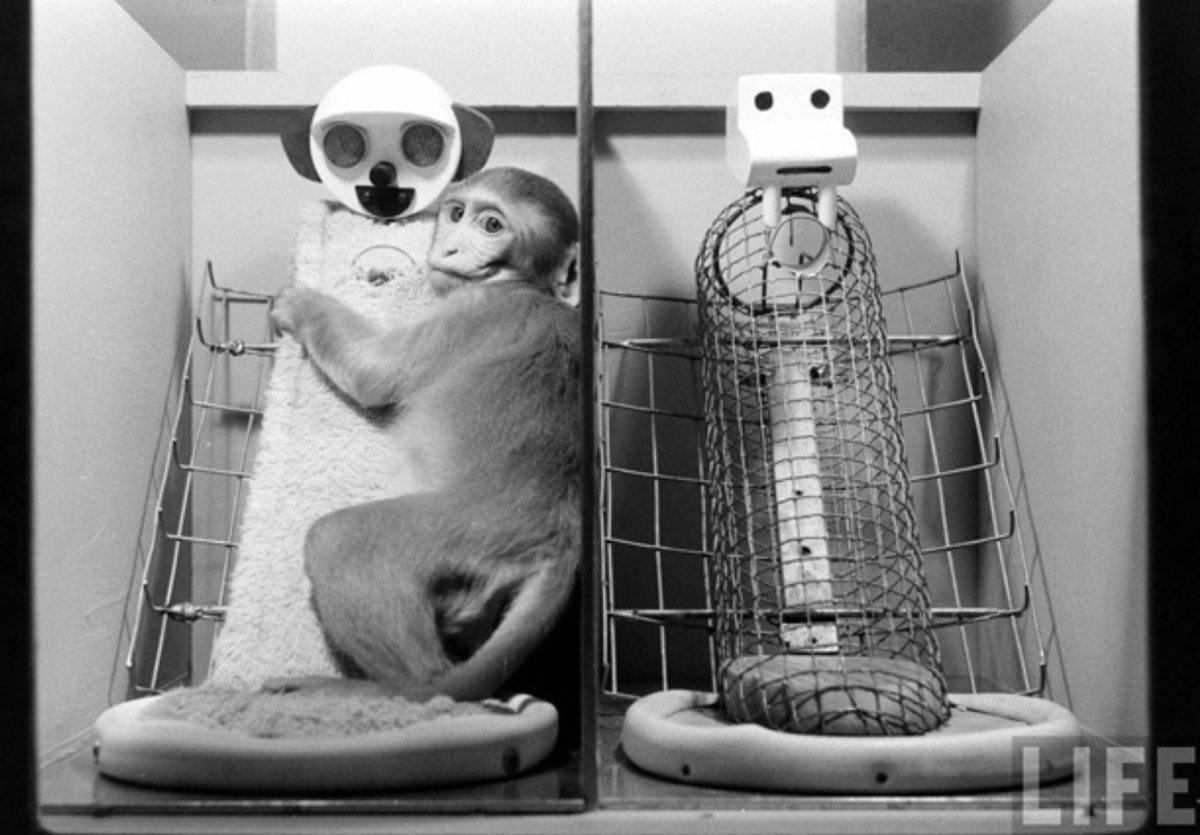
\includegraphics[width=0.95\linewidth]{images/Libro-img017.jpg}
  \begin{minipage}{\linewidth}
    \caption{Esperimento di Harry Frederick Harlow}
  \end{minipage}
\end{wrapfigure}

All'epoca dell'esperimento, nel 1958 si pensava che il legame tra madre e
figlio dipendesse in misura maggiore per il neonato da un soddisfacimento dei propri desideri primari, quindi di
mangiare e bere. Harry Frederick Harlow per il suo esperimento prenderà dei neonati di macachi invece di umani, siccome
sono autonomi nel movimenti già tra i 2 e i 10 giorni di vita e dimostrano affettività in modo simile a noi. Harlow
costruisce poi due madri surrogate dove la base è un cilindro fatto da una rete metallica e una testa di legno. Una
ricoperta da un panno caldo e morbido l'altra dotata di un meccanismo per nutrire il piccolo.
L'esperimento, è stato riproposto diverse volte e in alcuni casi dotavano la “madre morbida” anche
del dispositivo di nutrimento. In qualunque caso i piccoli di macaco hanno sempre scelto la “mamma morbida” spostandosi
verso l'altra solo quando avevano fame.

Questa è per Harlow una scoperta sensazionale, ne deduce che non c'entra nulla il soddisfacimento
della fame e della sete. La vera funzione dell'allattamento, è quella di avere un contatto intimo
con la madre. Anche in momenti di paura, indotta con un giocattolo meccanico i piccoli macachi si rifugiavano sempre
dalla “mamma morbida”. Nei momenti di tranquillità i macachi si sentivano liberi di scoprire
l'ambiente circostante solo in presenza della madre surrogata. Quando la madre viene tolta
dall'ambiente del macaco, quest'ultimo si mostra impaurito restando
accovacciati e iniziando a dondolare. Harlow mette così in crisi le teorie dell'epoca
sull'attaccamento ma anche a livello socioeconomico, minando la certezza assoluta che le madri
debbano restare a casa dal lavoro dopo il parto, in quanto, l'uomo può soddisfare lo stesso
bisogno affettivo del neonato. Harlow addirittura conclude dicendo che in futuro l'allattamento
diventerà un lusso che potrà permettersi solo chi può non lavorare.
\end{mdframed}

\bigskip

Purtroppo anche questo è stato un esperimento un po' crudele, di cui abbiamo diverse testimonianze
video\endnote{\protect\url{https://www.youtube.com/watch?v=\_O60TYAIgC4} }
\endnote{\protect\url{https://www.stateofmind.it/2016/04/attaccamento-esperimento-di-harlow/} }. 

\subsection{Quando è finita?}
Ma come si fa a capire quando una relazione è finita? A volte ci siamo talmente dentro da non poter vedere in maniera
obiettiva, da un punto di vista esterno come stiamo vivendo. La paura di restare soli ma anche la routine,
l'abitudine di una relazione ci porta a vedere quella come la nostra normalità. Anche se di
normale non è rimasto più molto, finendo per accettare situazioni asfissianti e tossiche. 


\bigskip

Di seguito alcuni
segnali\endnote{\protect\url{https://www.vice.com/it/article/8qjvq5/come-capire-quando-una-relazione-agli-sgoccioli} }:

\begin{itemize}
\item Il primo e più importante: Quando ci sentiamo continuamente messi sotto giudizio, quando dobbiamo continuamente
dimostrare qualcosa e che la relazione non ci sta potenziando ma ci sottrae energie.
\item I litigi sono più frequenti e immotivati 
\item Nelle discussioni il problema è sempre l'altro o sei sempre tu
\item Se non si riesce a trovare mai il tempo per stare assieme 
\item Il sesso diventa freddo
\item Cominci a non avere più interesse di cosa pensa o sente l'altro
\item Smettete di parlare del futuro
\item Quando ti succede una cosa bella, non è più la prima persona a cui lo dici
\item Abbracciarlo o avere un contatto fisico ti fa rabbrividire nel profondo
\item Fantastichi su una vita da solo o letteralmente con chiunque altro
\item Non ti interessa fare pace dopo aver litigato
\end{itemize}

\bigskip

Tutti noi attuiamo comportamenti tossici, in tutte le relazioni, quelle famigliari, di amicizia, sentimentali e, sarà
così per sempre, ma se impariamo a riconoscerli possiamo tentare di intervenire e
limitarli\endnote{\protect\url{https://www.ted.com/talks/katie\_hood\_the\_difference\_between\_healthy\_and\_unhealthy\_love/transcript?language=it}
}:

\begin{itemize}
\item Intensità: Avviene quando vi sentite soffocati, può succedere in diversi modi, inconsciamente, anche con le
migliori intenzioni. Per esempio quando il vostro partner vi dice “ti amo” prima che siete pronti, o per via dei
continui messaggi e telefonate. Dovete chiedervi se vi sentite a vostro agio con il ritmo della vostra intimità o dello
stile di vita che si sta creando. Pensate di avere il vostro spazio? Le vostre richieste vengono rispettate?
\item Isolamento: il partner vi sottrae da amicizie, passioni, famiglia, facendo commenti sulle vostre compagni o sui
vostri famigliari, facendo insorgere il germe del dubbio anche se infondato. Bisogna rimanere indipendenti per non
perdere la nostra identità e, incoraggiare il partner a fare tutto quello che faceva prima di conoscerci. 
\item Gelosia: riconoscere nel partner possessività, sospetto e rifiuto di ascoltarvi ogni volte che cercate di
rassicurarlo/a che non ci sia nulla da temere.
\end{itemize}
\begin{mdframed}[linewidth=1pt]
Marcel Proust scrivendo La prigioniera porta il protagonista a rinchiudere Albertine per gelosia, la cui attrazione per
lei successivamente scese. In questo paradosso dell'amore siamo gratificati e attratti dal partner
che sceglie noi, solo nella misura in cui lui o lei è libera ma, in quanto libera, può \ decidere di non sceglierci
più.

{\selectlanguage{italian}
La gelosia inoltre, per qualcuno è conferma dell'amore verso di noi, ma se troppa e protratta nel
tempo, ci porterà a desiderare proprio ciò che il partner vuole prevenire. Se siamo fedeli ma il partner non si fida di
noi e ce lo ribadisce continuamente buttandoci addosso i suoi dubbi e le sue insicurezze, succede che, appena si
presenterà l'occasione, la coglieremo. Perché, per essere trattati in questo modo pur restando
fedeli, conviene non esserlo e venir trattati come tali.}

{\selectlanguage{italian}
In un caso riportato in Amore e disamore\endnote{\protect\url{https://www.amazon.it/dp/8833316432} }, a fine terapia di coppia dove
lei ha tradito lui, quest'ultimo, ritrovata la serenità, si trova a dire alla sua compagna,
facendole l'occhiolino, come gesto d'intesa: “esci pure e, divertiti”. Il
terapeuta gli fa notare che, senza saperlo, questo gesto è stato molto strategico, perché così dicendole ha realizzato
un paradosso comunicativo: 'Se sono io a spingerti fra le braccia di un altro, non solo ti tolgo
la componente trasgressiva, ma mi dimostro molto sicuro di me stesso'.}
\end{mdframed}

\begin{itemize}
\item Denigrazione: Prima i discorsi erano divertenti, interessanti, sereni poi diventano meschini e mortificanti. Prese
in giro e battute che feriscono e, quando provate a spiegare che vi siete sentiti feriti, non vi ascolta, dite che
state esagerando e di non rompere. Quel genere di parole che tappano la bocca. Le parole del partner dovrebbero farvi
sentire sostenuti, incoraggiati, più sicuri e, non il contrario.
\item Instabilità: Commenti carichi d'odio seguiti da scuse e, la promessa che non ricapiterà più.
Minacce, riatti, di cosa succederà a me o te se ci lasciamo. Queste montagne russe non ci fanno capire la tossicità di
un rapporto quando diventano intrinseche della relazione stessa.
\end{itemize}

\bigskip

Ma quando finisce una relazione, riusciamo a migliorare per la prossima? E a non riproporre più gli stessi comportamenti
tossici? In generale no. Tendiamo a ripetere, nel tempo, lo stesso modello relazionale originale, poiché fanno parte di
noi e del nostro modo di relazionarci\endnote{Johnson, M. D., \& Neyer, F. J. (2019). (Eventual) stability and change
across partnerships. Journal of Family Psychology, 33(6), 711–721. doi:10.1037/fam0000523
\protect\url{https://pubmed.ncbi.nlm.nih.gov/30802084/} \ }
\endnote{\protect\url{https://www.stateofmind.it/2019/09/relazioni-sentimentali-cambiamento/} }. Però, è possibile! Solo se
accettiamo e diventiamo consapevoli di noi stessi e dei nostri difetti, in modo da prestare più facilmente attenzione,
quando questi nostri comportamenti si manifestano e, a quel punto trovare modi per intervenire. 

Quando una relazione finisce siamo attratti dal fuggire il dolore, che ha invece motivo d'esserci,
solitamente in modi dannosi, dal chiodo scaccia chiodo all'odiare tutto ciò che è stato. Se
impariamo a stare nel dolore, senza giudizio, possiamo portare a casa qualcosa per il futuro.
L'importante è monitorare che questi pensieri non sfuggano di mano e quando ci accorgiamo che
stiamo rimuginando, rimasticando all'infinito gli stessi contenuti, riportiamo
l'attenzione su quello che stavamo facendo, senza criticarci e magari darci una
mezz'ora al giorno, con un orario preciso, dove quei pensieri sono consentiti, anche scrivendo e,
evitarli per il resto della giornata.


\bigskip

Raffaele Morelli ricorda che la crisi non è mai crisi di coppia, ma crisi di uno degli elementi della coppia. Per curare
una crisi di coppia bisogna partire da curare noi stessi, dedicando più tempo non al dialogo nella coppia ma a quello
con noi stessi. Dedichiamoci più tempo evitando di pensare che tutto tornerà come prima. Non succederà, dobbiamo sapere
che la nostra relazione andrà in altri territori in altre direzioni inesplorate.


\bigskip
\begin{mdframed}[linewidth=1pt]
I maschi pensano solo a quello!

No, ma probabilmente ci pensano di più rispetto alle femmine. I motivi principali sono due. Il primo dipende da un
fattore religioso e culturale che associa la vergogna al sesso. Con il tempo sicuramente il tema sta diventando sempre
meno un tabù, per entrambi i sessi, ma evidentemente c'è ancora un divario che pone la donna in
una misura di maggiore vergogna rispetto all'uomo. Il secondo motivo è evolutivo. Biologicamente
non siamo troppo diversi dal primo homo sapiens sapiens che doveva lottare per la propria sopravvivenza. Al fine di
conservare la specie, la riproduzione è necessaria, ma sicuramente per la femmina il compito è sicuramente più gravoso
e rischioso. Infatti una gravidanza richiede più energie, risorse, si può morire di parto, anche quando nasce il
bambino, c'è l'allattamento, le cure, ecc… Ora abbiamo dei metodi per evitare
la gravidanza, ma a livello più inconscio, più primitivo, ragioniamo ancora allo stesso modo. Quindi una donna quando
decide di riprodursi mette sul piatto della bilancia dei rischi, quelli appena elencati, e un guadagno, la
conservazione della specie. Un uomo non ha rischi, quindi non ha nessun buon motivo di perdere
l'occasione di conservazione della specie\endnote{Trivers, R.L. (1972). Parental investment and
sexual selection. In B. Campbell (Ed.), Sexual selection and the descent of man (pp. 136–179). Chicago, IL: Aldine}
\endnote{\protect\url{https://www.stateofmind.it/2020/03/attrazione-sessuale-riconoscimento/} }.

Diversi studi mostrano come il desiderio sessuale all'interno della coppia tende a diminuire
maggiormente per le femmine rispetto ai maschi, soprattutto dopo la gravidanza e il parto. Questo può portare al
declino della soddisfazione relazionale della coppia\endnote{McNulty, J. K., Maxwell, J. A., Meltzer, A. L., \&
Baumeister, R. F. (2019). Sex-Differentiated Changes in Sexual Desire Predict Marital Dissatisfaction. Archives of
sexual behavior, 48(8), 2473-2489. \protect\url{https://pubmed.ncbi.nlm.nih.gov/31471791/} }
\endnote{\protect\url{https://www.stateofmind.it/2020/04/cambiamento-desiderio-sessuale/} }.
\end{mdframed}

\subsection{Figli}
Non ne so molto di figli, ma ho collezionato comunque qualche articolo che mi sembrava interessante. Non si sa mai.

Frasi diseducative\endnote{\protect\url{https://www.vice.com/it/article/k7akpm/frasi-genitori-diseducative} \ }

\begin{itemize}
\item Abbandono

\begin{itemize}
\item Frasi

\begin{itemize}
\item “Se non ti sbrighi ti lascio qui”
\item “Se fai così la mamma/il papà va via”
\end{itemize}
\item Problema: Questo fa emergere l'angoscia da abbandono, che per un bambino è peggio della paura della morte.
\item La soluzione: Il nostro obiettivo non è far sentire abbandonato nostro figlio ma che si velocizzi e non si
disperdi. Giriamo la frase al positivo, invece di “se non fai…” diventa invece “se fai questo…”, o ancora dire “ok, ti
do dieci minuti per finire con l'altalena e poi andiamo”, aiutano a imparare concetti importanti
come il compromesso.”
\end{itemize}
\item Minacce e ricatti

\begin{itemize}
\item Frasi

\begin{itemize}
\item {\textquotedbl}Guarda che se urli ti porto dallo psicologo/in collegio{\textquotedbl}
\item “Se non ti comporti bene vedi cosa ti faccio”
\item “Se non fai i compiti, non ti compro quel giocattolo”
\end{itemize}
\item Problema: Premi o punizioni non sono funzionali perché il bambino pone attenzione non sul suo comportamento ma
sulla punizione/premio, quindi cercherà di soddisfare le aspettative dell'adulto, ma senza capirne
davvero il motivo
\item La soluzione: Sottolineare i comportamenti positivi, in modo che il bambino si soffermi a riflettere su questa
acquisizione positiva”. Allo stesso modo fare per i comportamenti negativi, spronando il bambino a migliorarsi. Invece
di dire: “non puoi giocare al Pc perché non hai finito i compiti”, anticipare dicendo: \ “non appena avrai finito i
compiti, potrai giocare.” Un metodo più manipolatorio è invece porre una scelta dove la risposta preferibile è messa al
secondo posto. Secondo uno studio dell'Università della California-Irvine, ponendo domande come: “vuoi il dado rosso o
quello blu, il robot o il trenino... ?” I bambini hanno optato per la seconda scelta l'85\% delle volte, anche quando i
termini della stessa domanda venivano invertiti. Mentre per gli adulti è più facile il contrario, ovvero, che scelgano
la prima opzione per un effetto chiamato “effetto primacy”. 
\end{itemize}
\item Insegnamenti sulla morale

\begin{itemize}
\item Frasi:

\begin{itemize}
\item “È un mondo difficile, è meglio se lo impari subito”
\item {\textquotedbl}Mangia tutto che nel mondo ci sono bambini che muoiono di fame{\textquotedbl}
\item “Quando sarai grande potrai fare quello che vuoi, adesso no”
\end{itemize}
\item Problema: Secondo gli esperti, le frasi sulla morale sono più una esternazione delle difficoltà che prova
l'adulto, ma traslate sul bambino spesso in negativo e/o in maniera punitiva.
\item Soluzione: Per insegnare la morale può essere una buona idea raccontare o leggere delle storie.
\end{itemize}
\item Confronti con coetanei e adulti

\begin{itemize}
\item Frasi:

\begin{itemize}
\item “Perché non sei come tuo cugino, che è così ubbidiente?{\textquotedbl}
\item “Sei come tuo padre/tua madre”
\item “Faccio io, che tu non sei capace”
\end{itemize}
\item Problema: rischiamo di intaccarne l'autostima e la sicurezza del bambino, necessarie per
affrontare il futuro. 
\item Soluzione: Paragonare il bambino di oggi con quello di ieri, ad esempio: “sono contento perché al parco hai
giocato con tutti i bambini, e avete condiviso i giochi”.
\end{itemize}
\item Stereotipi e paura del giudizio sociale

\begin{itemize}
\item Frasi:

\begin{itemize}
\item “Non piangere, non vorrai che dicano che sei una femminuccia”
\item “Tu sei una signorina, non devi fare così”
\item “No questo giocattolo non è adatto per te, compriamone un altro” 
\end{itemize}
\item Problema: Gli schemi sono rassicuranti e sapere che nostro figlio/a si comporta come dovrebbe comportarsi, ci fa
sentire dei bravi genitori, ma non permette all'unicità del bambino di emergere
\item Soluzione: Individuare se il bambino si comporta in maniera oggettivamente sbagliata o solo socialmente sbagliata.
\ Nel secondo caso possiamo lasciarlo esprimere. Nel primo caso spiegare che si comprende il suo stato
d'animo ma il suo comportamento non è accettabile. In altre parole dire: “hai sbagliato” e non
“sei sbagliato”. Fare capire che anche gli adulti sbagliano e che non c'è crescita senza errore, ma che è importante
rimediare ai propri sbagli.
\end{itemize}
\end{itemize}
Divorzio

In Intelligenza emotiva per la coppia\endnote{\protect\url{https://www.amazon.it/dp/8817069124} } John Gottman scrive che è
decisamente dannoso allevare bambini in una casa in cui si scatenano le dinamiche di ostilità dei genitori. Un
tranquillo divorzio è meglio di un matrimonio conflittuale. 

Internet e videogiochi

Al massimo un'ora al giorno durante la settimana, 4 durante i week-end. Questo è ciò che è emerso da uno studio del
Center for Gambling Studies della Rutgers University pubblicato su Computers in Human Behaviour. Analizzando i dati del
China Education Panel Survey, dove sono stati intervistati e seguiti circa 10.000 studenti delle scuole medie, i
ricercatori hanno mostrato che i bambini che usavano Internet, social media o videogiochi per 4 o più ore al giorno
avevano una probabilità 4 volte maggiore di saltare la scuola rispetto a quelli che non lo facevano, mostrando livelli
di impegno scolastico inferiori. Viceversa, chi usava Internet e videogame per meno di un'ora al giorno, sperimentava
meno noia a scuola, ottenendo migliori risultati. 

Film violenti

Guardare film con un po' di violenza, come quelli dei super eroi con i bambini può andar bene a patto che poi si
spieghino le conseguenze della violenza. Altrimenti, se non lo si fa, il bambino interpreta il silenzio assenso dei
genitori come tacita approvazione di quello che è appena stato visto.

Mangiare

Vuoi che tuo figlio mangi gli spinaci? Non serve forzarlo, ma dimostragli quanto ti piacciono. In generale, anche al di
fuori del mangiare, il buon esempio funziona anche per altre cose, come ad esempio se vuoi che leggano di più.

Dormire

Per aiutare i bambini a dormire meglio, è importante considerare diverse strategie. Prima di tutto, è consigliabile
ridurre i riposini diurni e stabilire una routine che comprenda attività rassicuranti come la lettura di una storia o
il bagno. Una luce soffusa può creare un'atmosfera tranquilla nella stanza. Inoltre, insegnare ai bambini a dormire
autonomamente è un obiettivo importante, anche se potrebbe richiedere pazienza. Infine, è essenziale essere flessibili
e valutare se sia il momento giusto per separarsi durante il sonno, ascoltando le esigenze individuali del bambino.

\clearpage\section{Ecologia}
Il cambiamento climatico e il sovrappopolamento sono tra le due più grandi sfide dell'era
contemporanea. Non possiamo sapere quando accadrà, ma accadrà, le stime più catastrofiste riescono a collocarlo tra il
2030 e il 2050. Alcuni paper come quello scritto dal professore Jem Bendell, che si occupa di sostenibilità
all'Università di
Cumbria\endnote{\protect\url{https://jembendell.com/2018/07/26/the-study-on-collapse-they-thought-you-should-not-read-yet} } mostra
uno scenario drammatico, i cambiamenti climatici hanno già raggiunto una soglia irreversibile e, gli effetti saranno
visibili per ognuno di noi, non soltanto nei luoghi più svantaggiati. Questo paper è talmente drammatico che vi chiedo
prudenza nel leggerlo in quanto diverse persone sono cadute in depressione, c'è chi è scappato in
campagna in attesa della catastrofe e chi è andato in terapia.


\bigskip

\subsection[Orologio dell{}'apocalisse]{Orologio dell'apocalisse}
Doomsday Clock in inglese, è un orologio metaforico creato attorno agli anni cinquanta
dall'università di Chicago che indica la vicinanza alla fine dell'umanità,
rappresentata dalla mezza notte. Ogni anno studiosi e ricercatori ricalcolano quanti minuti mancano alla mezza notte,
ovvero alla fine dell'umanità tirando in avanti o indietro le lancette. Inizialmente
quest'orologio rappresentava solo la guerra atomica dal 2007 considera qualsiasi evento tra cui il
riscaldameo globale. Il 1991 è stato il momento più lontano dall'apocalisse, ben 17 minuti,
siccome in quell'anno viene firmato il trattato di riduzione delle armi strategiche, L'URSS viene sciolta, finisce la
guerra fredda. il 1991 è stato l'anno migliore anche grazie ai due anni precedenti dove USA e URSS hanno firmato il
Intermediate-Range Nuclear Forces Treaty, Firma del trattato INF, Cade il muro di Berlino, Alcune nazioni dell'Europa
dell'est diventano indipendenti dall'URSS. L'anno peggiore invece è stato il 2020, per il continuo
riarmo nucleare, e la mancanza di azioni da parte delle grandi potenze nel contrastare i cambiamenti climatici.

\begin{figure}[H]
  \centering
  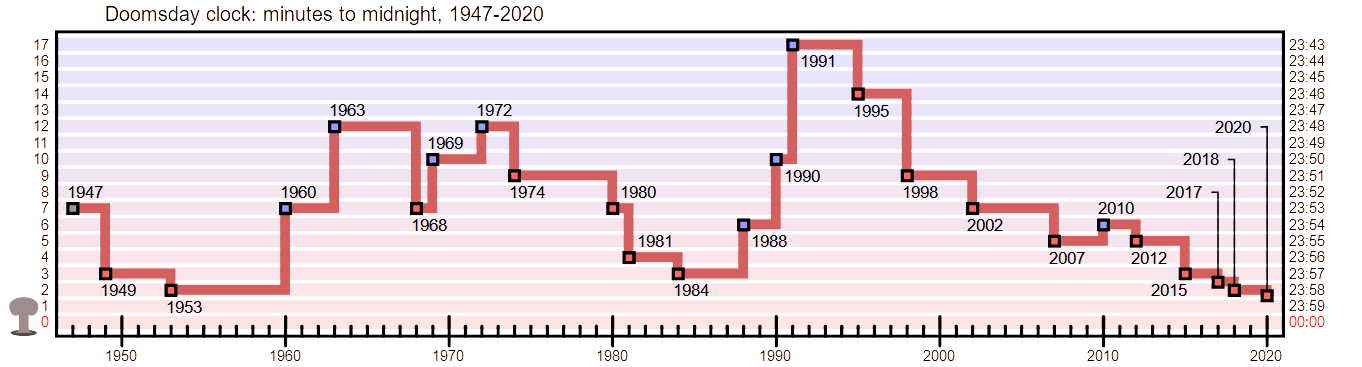
\includegraphics[width=0.95\linewidth]{images/Libro-img018.png}
  \caption{Di Fastfission 15:00, 14 April 2008 (UTC) - Opera
propria, Pubblico dominio, \protect\url{https://commons.wikimedia.org/w/index.php?curid=1575536}}
\end{figure}

\subsection{Overshoot Day}
L'overshoot day è il giorno in cui noi esseri umani abbiamo consumato più di quanto la Terra abbia
prodotto in un anno e, l'effetto è quello di aver prodotto più anidride carbonica di quanta se ne
sia assorbita.

Nel 2019 l'overshoot day è stato il 29 luglio, questo vuol dire che per 5 mesi siamo stati in
debito con la terra e abbiamo utilizzato risorse che si sono accumulate molti anni fa quando riuscivamo ad essere in
credito col pianeta.

Questa data in realtà è peggio di quanto sembri, perché nel mondo ci sono gli occidentali con il loro tenore di vita e i
paesi del terzo mondo con utilizzo di risorse molto inferiori alle nostre.

L'overshoot oay dell'Europa nel 2019 è stato il 10 maggio e, per l'Italia il
15 maggio.


\bigskip

Consumiamo più legna di quanto non ne producano le foreste, mangiamo più animali di quanto il loro ciclo riproduttivo
riesca a farne nascere, consumiamo vegetali a un ritmo maggiore dei tempi necessari alla coltivazione. 

Come potete vedere da questo grafico l'ultima volta che siamo riusciti a consumare meno risorse di
quante ne siano state prodotte è stato il 1970, quando c'erano circa 3,7 miliardi di persone, da
allora il giorno si è avvicinato sempre di
più\endnote{\protect\url{https://www.overshootday.org/newsroom/press-release-july-2019-italian/} }.


\bigskip

Come vediamo l'overshoot day è legato al numero di persone presenti sul pianeta terra, se siamo
pochi, possiamo permetterci di consumare più risorse, nel 2050 la popolazione mondiale sarà circa 10 miliardi e il
tenore di vita sarà mediamente più alto per tutti, l'obiettivo sarà anche non avere più un terzo
mondo e l'unione di queste due porterà con sé una grande sfida da
affrontare\endnote{\protect\url{https://www.wired.it/attualita/ambiente/2015/08/13/overshoot-day-terra/} }.


\bigskip

Sul sito ufficiale potete calcolare il vostro personale overshoot day:

www.footprintcalculator.org 

e vedere l'impronta ecologica di ogni stato:

data.footprintnetwork.org


\bigskip

\begin{figure}[H]
  \centering
  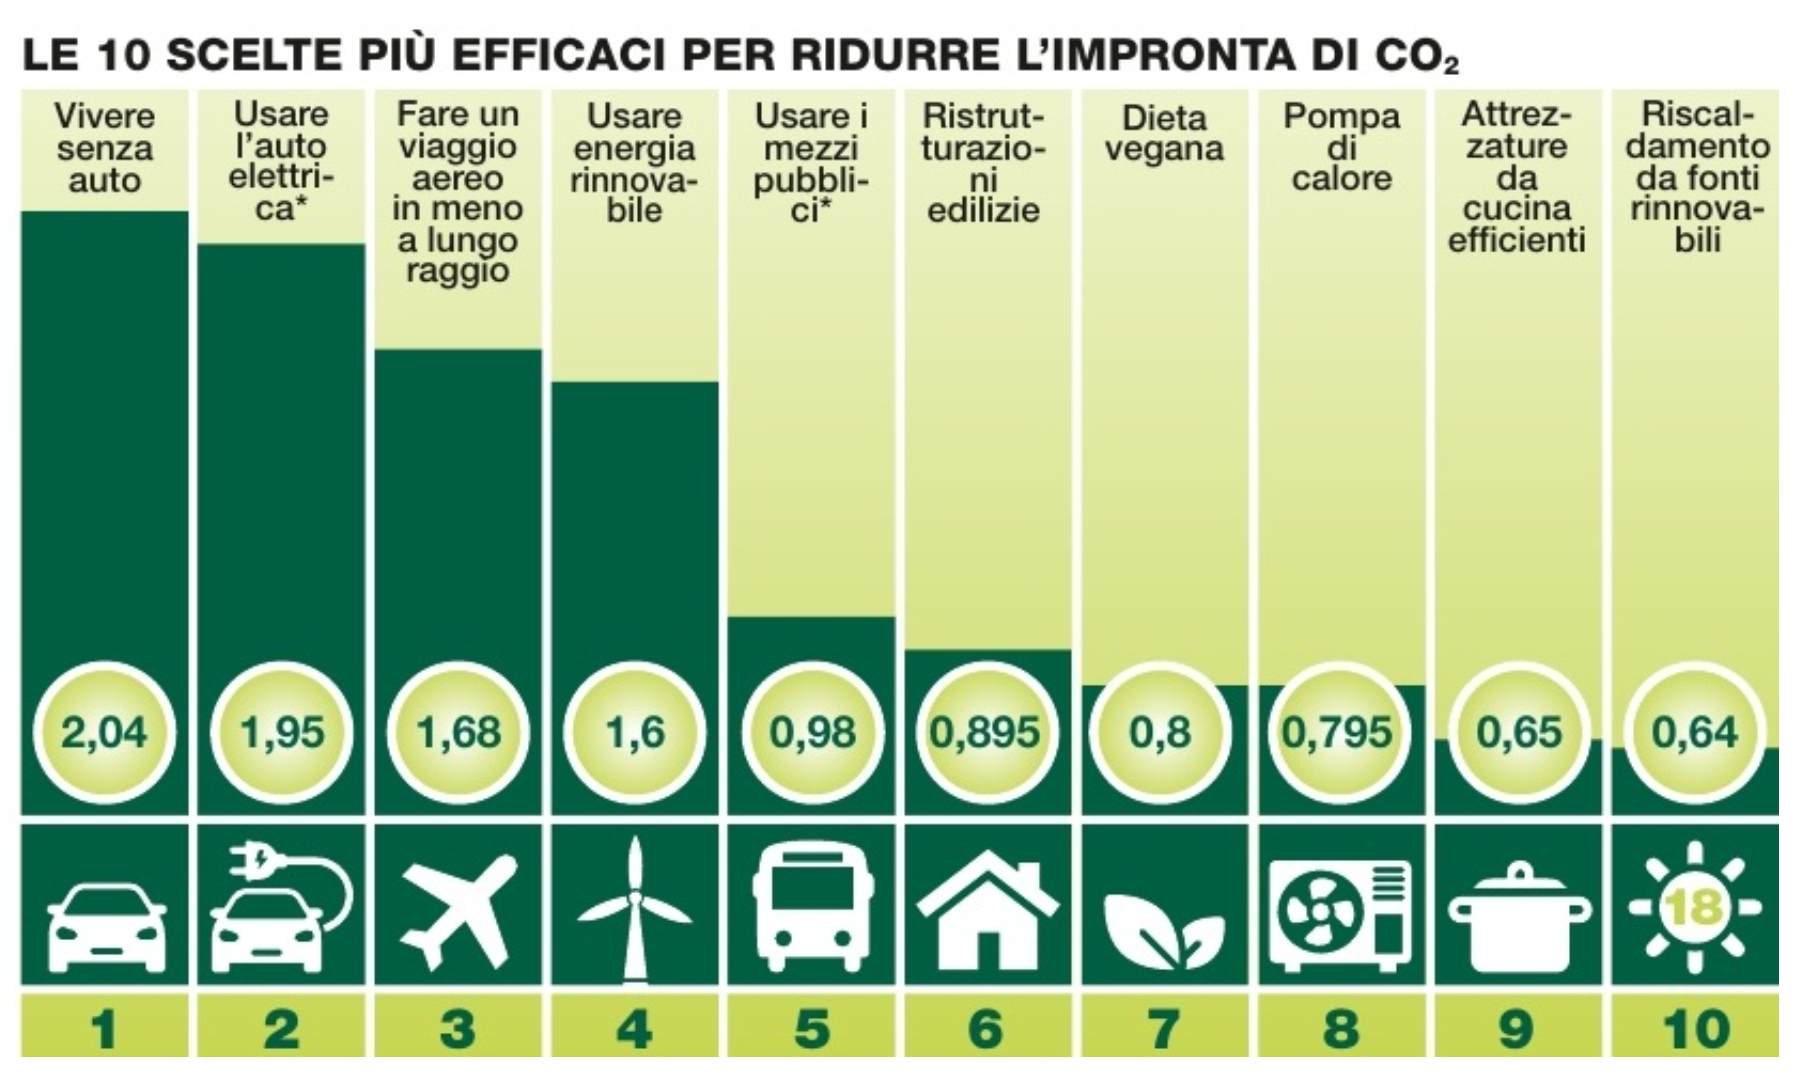
\includegraphics[width=0.95\linewidth]{images/Libro-img019.jpg}
  \caption{Tratto da un ritaglio di giornale (Focus)}
\end{figure}

Nella storia della terra ci sono state diverse ere, ben cinque, che hanno portato a intere estinzioni di massa. Secondo
uno studio pubblicato da Proceedings of the National Academy
Sciences\endnote{\protect\url{http://www.pnas.org/content/early/2017/07/05/1704949114} } stiamo vivendo in questo momento la sesta
estinzione di massa dovuta dallo {\textquotedbl}spaventoso assalto alle fondamenta della civilizzazione
umana.{\textquotedbl}. La ragione di questa nuova estinzione dipende interamente dall'uomo,
bracconaggio, il surriscaldamento globale, il consumo inarrestabile di suolo e, crescita della popolazione. La
biodiversità si sta riducendo a una velocità di cento volte superiore a quella considerata “normale” e questo numero è
in continua crescita. Inoltre il problema non si riferisce solo a animali rari ma anche a specie molto comuni, infatti,
negli ultimi decenni è scomparso il 50 percento degli animali selvatici. La riduzione di biodiversità non è un problema
perché quando andremo allo zoo vedremo meno animali, ma perché innesca una serie di effetti a catena che ricadrà anche
sulla sopravvivenza dell'umanità stessa con conseguenze economiche e
sociali\endnote{\protect\url{https://www.vice.com/it/article/qv9jym/estinzione-massa-specie-animali} }.

Per la natura non è un problema l'estinzione umana o di altre specie, non ha un interesse a
salvarci. Quando non c'è più da mangiare pian piano si ridurranno le specie viventi finché non
torna un equilibro di “domanda e offerta” delle risorse e, l'equazione sarà nuovamente bilanciata.


\bigskip

Tra le varie iniziative è nato il
BirthStrikers\endnote{\protect\url{https://www.theguardian.com/lifeandstyle/2019/mar/12/birthstrikers-meet-the-women-who-refuse-to-have-children-until-climate-change-ends}
}, un movimento che pone la scelta dolorosa di non avere figli. Questa protesta viene fatta per diversi motivi. Secondo
numerosi scienziati, siccome ogni persona sulla terra ha dei consumi, produce rifiuti, va in macchina ecc… il
sovrappopolamento è uno dei problemi principali per la salute
terreste\endnote{\protect\url{https://www.vice.com/it/article/znj9g5/sos-soluzioni-scrittori-scienziati-esperti-ambiente-a11n3-753}
}.

\ Il 2050 è stata posta dagli esperti come la data dove se non riusciamo a cambiare radicalmente, il surriscaldamento
globale renderà una buona parte della terra un posto inospitale, così, alcune persone sentono la responsabilità di
mettere al mondo un figlio in un posto invivibile. Infine, una delle motivazioni più diffuse che porta alcune donne a
compiere questa scelta dolorosa è quella di protesta per spingere i governi ad
agire\endnote{\protect\url{https://www.vice.com/it/article/59nzxb/birthstrike-non-fare-figli-per-salvare-il-pianeta} }.

Nonostante la crescita globale sia più lenta rispetto agli anni passati, la popolazione continuerà a crescere fino al
2080, quando il mondo raggiungerà i 10,4 miliardi di abitanti. Una volta arrivati a questa soglia, il trend dovrebbe
invertirsi e la popolazione mondiale cominciare a diminuire.

Ancora più diffuso è il movimento no-fly dove persone rinunciano all'aereo come mezzo di trasporto
preferendo il treno.


\bigskip

\begin{table}[]
\begin{tabular}{lllll}
Mezzo di trasporto & Media di passeggeri & Emissioni (g CO2/(km * passeggeri) & & \\
Aeroplano & 88 & 285 & & \\
Nave & - & 245 & & \\
Grande macchina & 1,5 & 158 & & \\
Piccola Macchina & 1,5 & 104 & & \\
Moto & 1,2 & 72 & & \\
Pullman & 12,7 & 68 & & \\
Grande macchina & 4 & 55 & & \\
Piccola macchina & 4 & 42 & & \\
Treno & 156 & 14 & & \\
Bicicletta & 1 & 0 & & 
\end{tabular}
\end{table}

\bigskip

I dati\endnote{\protect\url{https://en.wikipedia.org/wiki/Environmental\_impact\_of\_transport} } indicano come il mezzo più
inquinante sia proprio l'aereo che produce, per un volo breve come Milano Roma in media 70
chilogrammi di anidride carbonica. Al secondo posto troviamo le navi da crociera, che inquinano altrettanto ma possono
portare più passeggeri e solitamente fanno meno chilometri, inquinando quindi leggermente meno. A seguire il trasporto
su gomma, quindi macchine, furgoni, camion, bus ecc… dove il rapporto di C02 prodotta per chilometro è sicuramente più
efficiente rispetto a navi e aerei, ma per via della loro numerosità e tempo di utilizzo sono i mezzi di trasporto ad
oggi più inquinanti. Infine abbiamo il treno che si conferma, con un ampio margine, il mezzo più ecologico, anche
rispetto alle auto elettriche per via dell'elevato numero di passeggeri che un solo mezzo può
trasportare. Come mezzo ancora più ecologico troviamo la bici che però non consente lunghi spostamenti. Sempre più
diffusa è la scelta di persone, che per spostamenti quotidiani utilizza il treno associato alle bici pieghevoli e
monopattini. In modo da coprire la quasi totalità della distanza in treno e concludere lo spostamento finale in bici.
La scelta del treno, riducendo le macchine in circolazione permette quindi, oltre alla diminuzione di CO2 di ridurre il
traffico, aumentare la sicurezza stradale e regalarci del tempo extra, siccome sul treno possiamo studiare, leggere,
guardare un film, dormire ecc…


\bigskip

\subsection{Cambiamento climatico}
Il cambiamento climatico è un tema molto discusso ma che ogni tanto ho l'impressione venga
sottostimato. Tra le critiche principali troviamo persone che non vedono la necessità di cambiare con fatica il proprio
stile di vita in quanto un paio di gradi in più farebbero anche piacere. Il problema principale è che il cambiamento
dell'equilibrio tra gli organismi che necessitano di particolari condizioni porterebbe un effetto
domino che arriverebbe anche a noi. Per esempio la morte di alcuni insetti ridurrebbe
l'impollinazione di diversi vegetali, di conseguenza ci sarebbe meno riduzione di anidride
carbonica, un ulteriore innalzamento della temperatura che ucciderebbe altri vegetali che magari mangiamo noi umani o,
che mangiano altri animali che rientrano nella nostra dieta. Ma gli esempi sono davvero innumerevoli e
tutt'ora se ne scoprono di nuovi. Un'altra percezione errata che si ha sul
cambiamento climatico è quella di sentire più freddo rispetto ad anni fa. Meno 33 gradi a Chicago, -35 °C in Nord
Dakota, venti freddi a -52 °C. C'è da fare una particolare distinzione tra meteo e clima. Il meteo
spiega quanto accade in un tempo spazio limitato. Mentre il clima si riferisce a tempi più lunghi,
nell'arco di 150 anni e globalmente. Inoltre abbiamo il vortice polare, che possiamo vederlo come
un anello di venti freddi che ruota attorno al Polo Nord. Con il surriscaldamento terreste questo vortice è diventato
irregolare disegnando onde più ampie in alcune aree e più ristrette in altre. Nei punti più ampi verranno quindi
coinvolte aree dove solitamente il meteo è più mite. 

Negli ultimi 70 anni alcuni scienziati hanno dimostrato che il clima si sta raffreddando, ma il resto della comunità
scientifica non si è mai ritrovata con questi dati, infatti 13 dei 14 anni più caldi si sono verificati proprio nel
ventunesimo secolo. Considerare solo la temperatura può essere fuorviante, abbiamo altri indici come lo scioglimento
dei ghiacci, l'innalzamento dei mari, ma anche questi possono essere travisati, qualcuno potrebbe
dire che negli ultimi anni i ghiacci sono aumentati del 40\%. Questa non è una notizia falsa, ma decontestualizzata, se
guardiamo infatti gli ultimi quarant'anni vedremo che la tendenza è comunque negativa.


\bigskip

\begin{figure}[H]
  \centering
  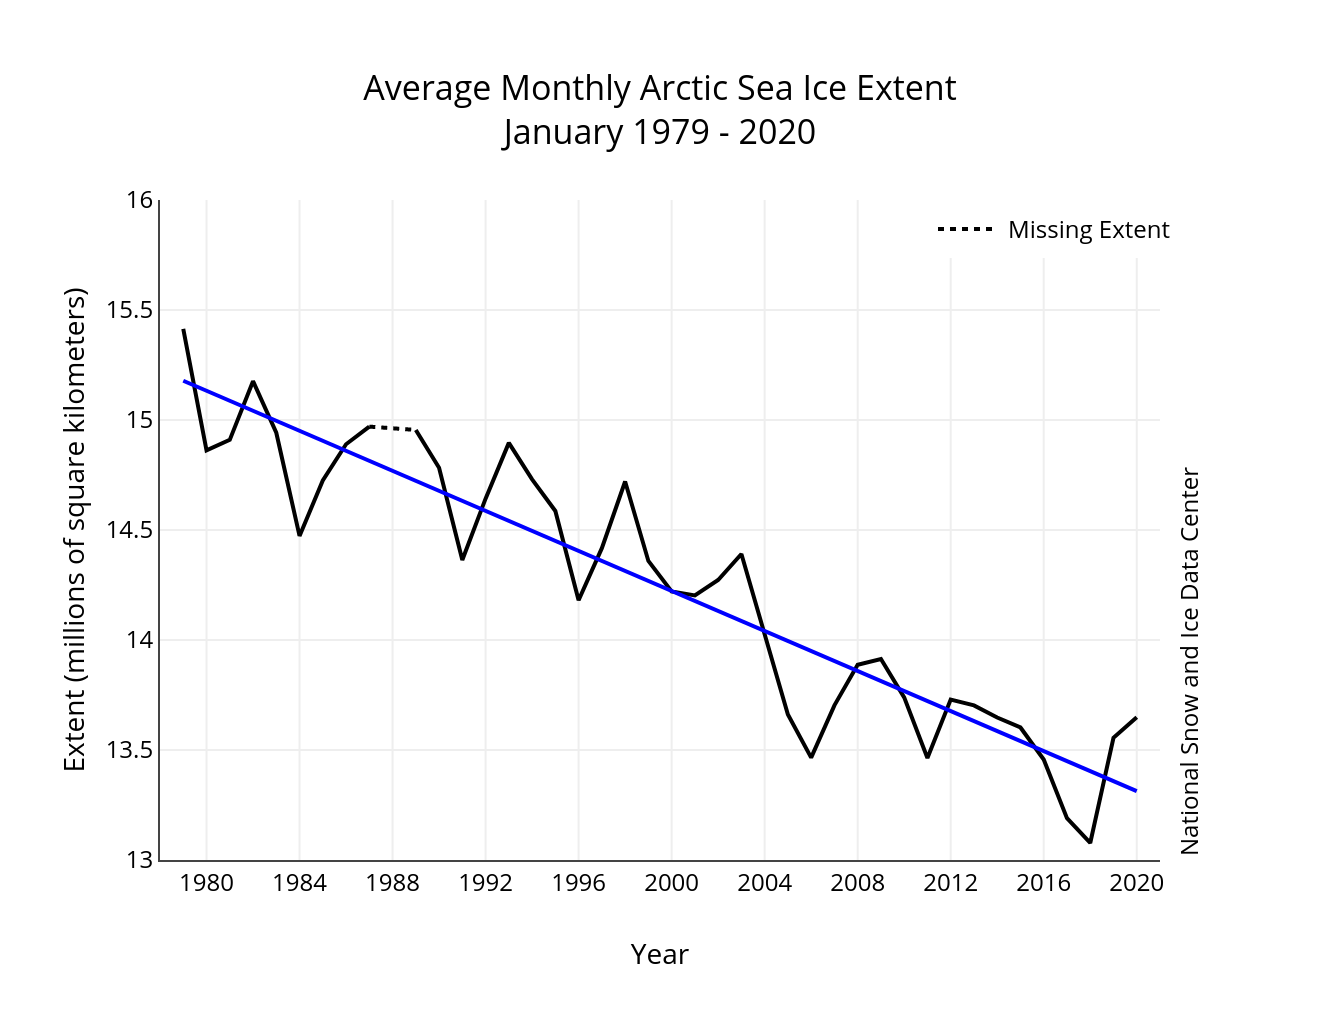
\includegraphics[width=0.95\linewidth]{images/Libro-img021.png}
  \caption{L'estensione mensile del ghiaccio di gennaio per il
periodo 1979-2020 mostra un calo del 3,15 percento per decennio. Credits: \href{https://nsidc.org/arcticseaicenews/2020/02/}{National Snow and Ice Data Center}}
\end{figure}

Il modo più giusto di guardare questo grafico è quindi la linea blu e non l'ultimo pezzo di linea
nera. Questo genere di lettura viene fatta su qualsiasi cosa, è un'arma usatissima in tutte le
forme di negazionismo, fake news e complotto. Un altro esempio? Ho trovato alcuni negazionisti del cambiamento
climatico che lo reputano dovuto all'aumento dell'attività solare più che
dalle attività umane, mostrando il seguente grafico decontestualizzato:

\begin{figure}[H]
  \centering
  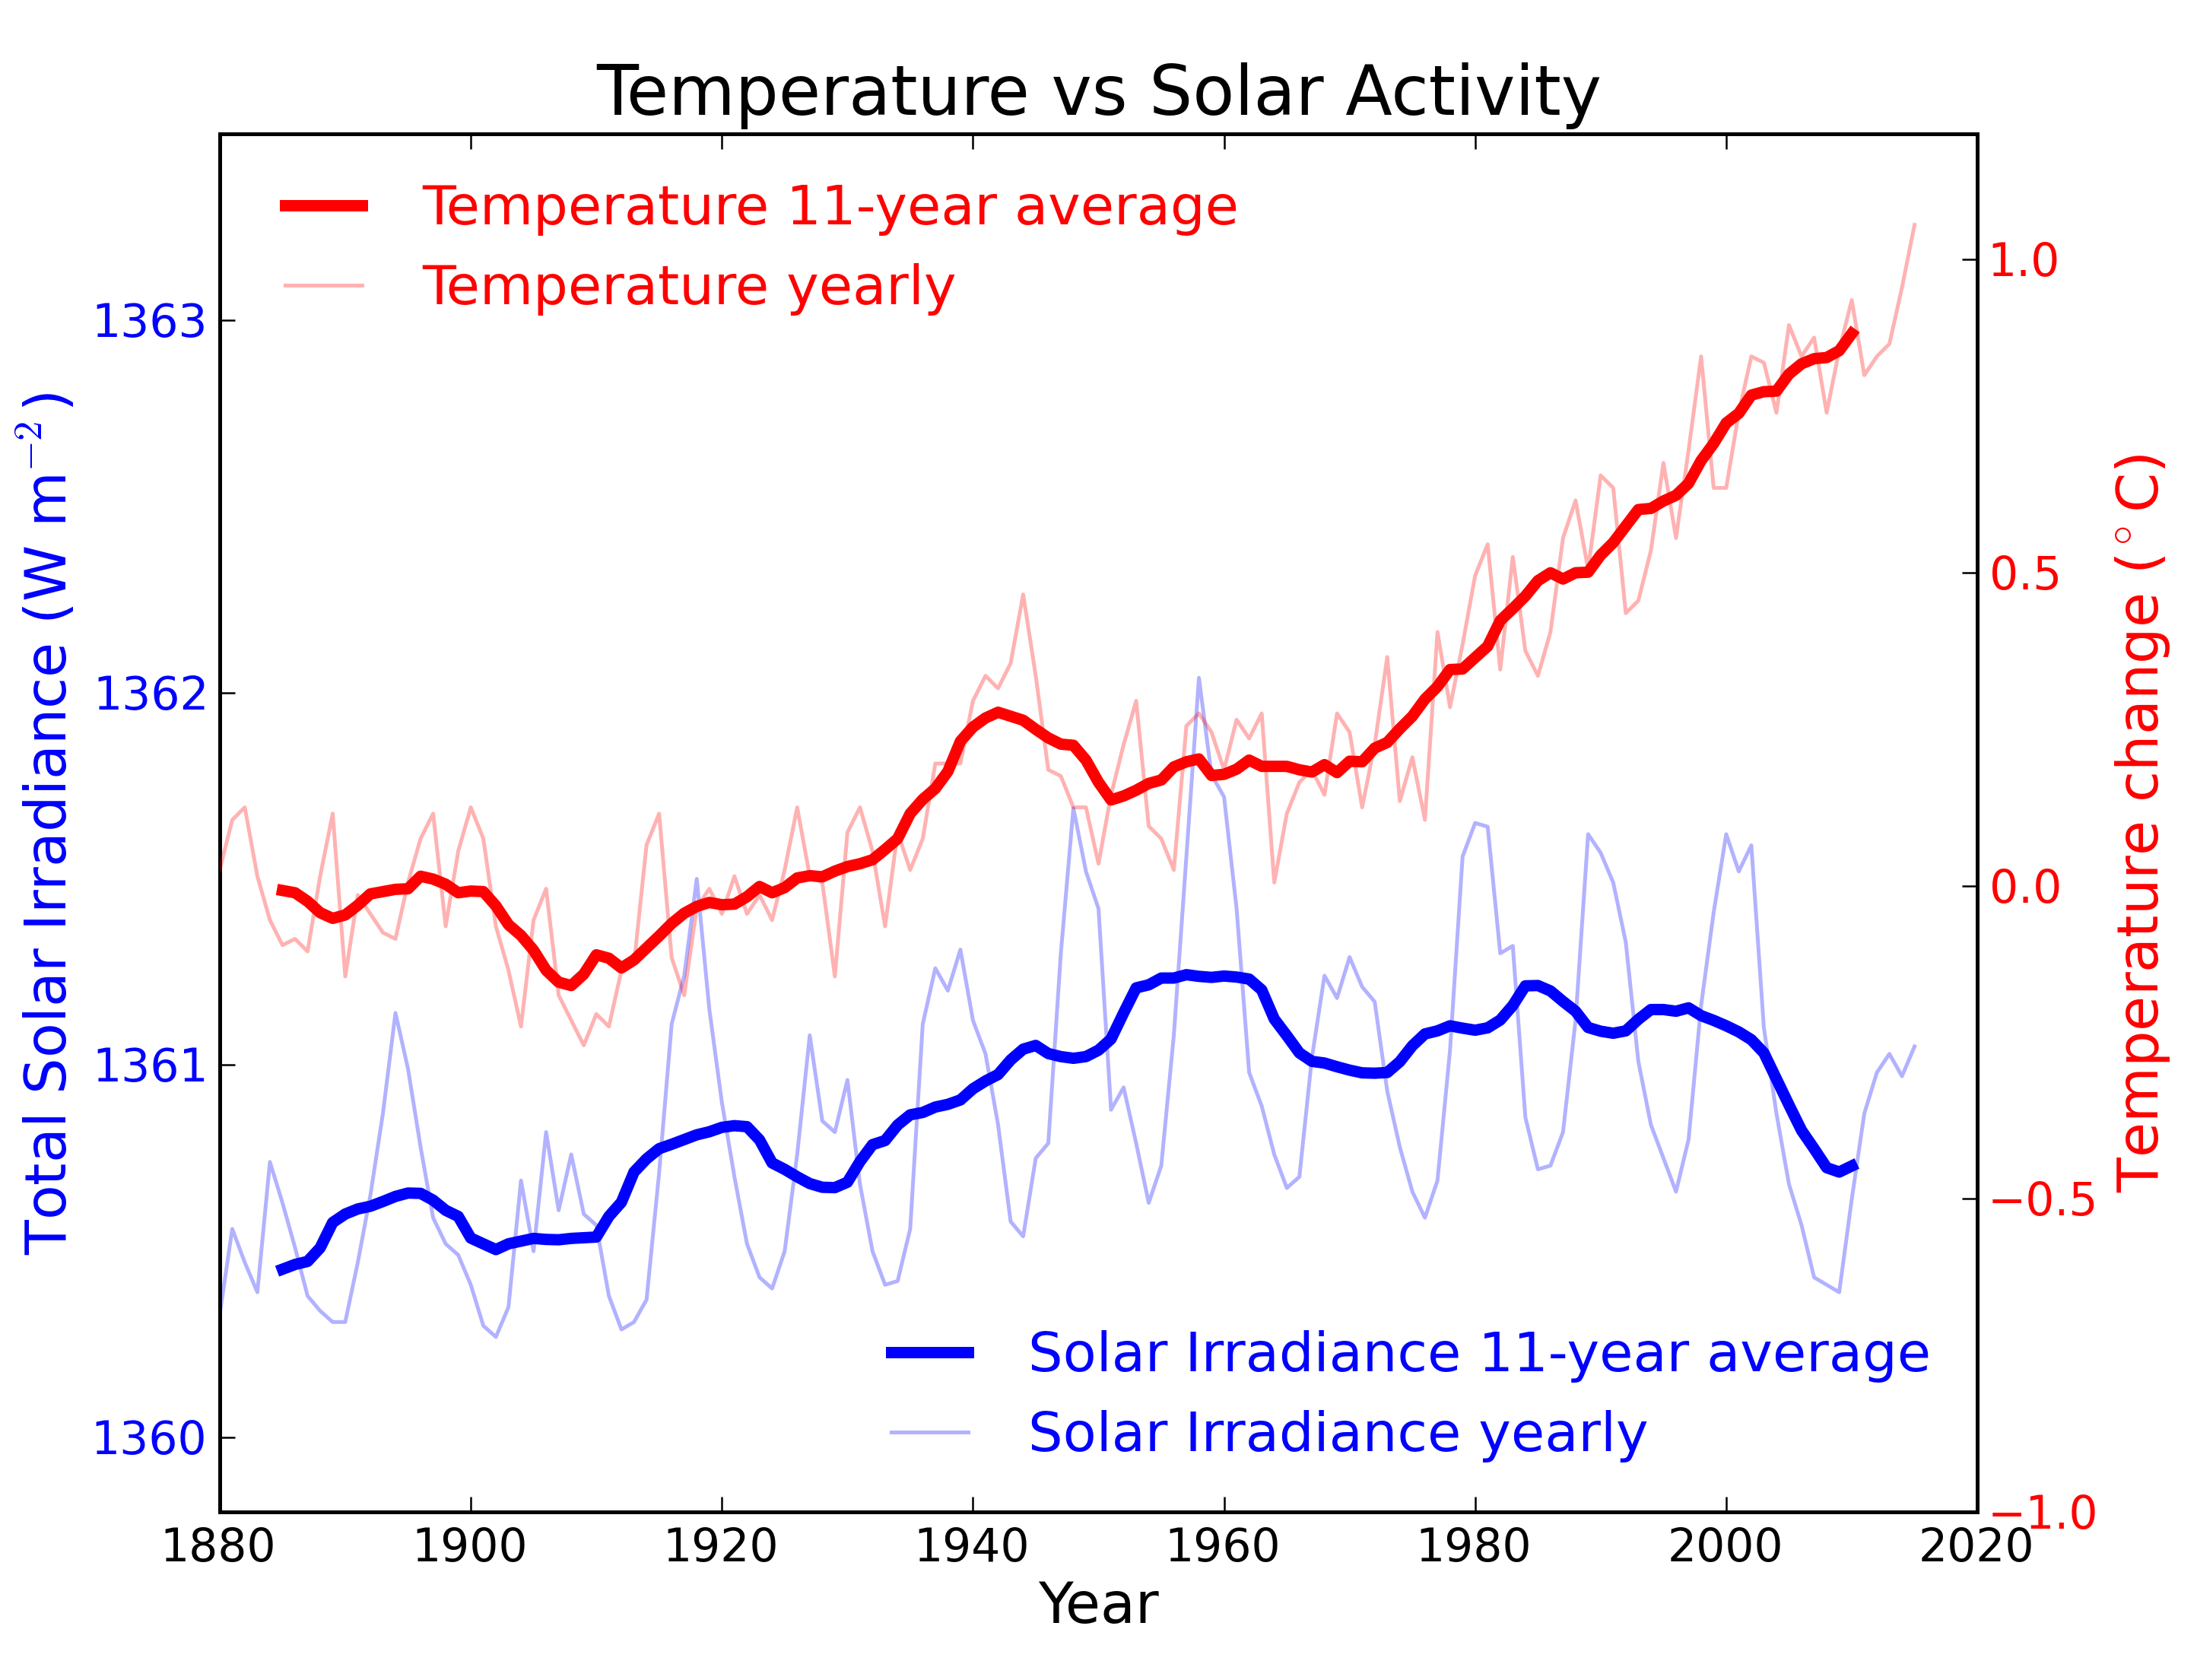
\includegraphics[width=0.95\linewidth]{images/Libro-img022.png}
  \caption{Credits: \href{http://data.giss.nasa.gov/gistemp/tabledata/GLB.Ts+dSST.txt}{NASA GISS}}
\end{figure}

In che modo si può travisare questo grafico? Tagliandolo fino agli anni 50 o non mostrandolo affatto. Infatti la linea
blu mostra che dagli anni 30 agli anni 50 c'è stato un aumento di attività solare che ha portato a
un aumento della temperatura terreste, ma quando si è stabilizzata la temperatura ha continuato a salire. Questi
grafici sono stati travisati con la Fallacia dell'evidenza soppressa e della conclusione sbagliata.

Il maggiore responsabile è quindi la CO2 di cui però si potrebbe obbiettare che gli esseri umani sono responsabili della
produzione di sole 30 gigatonnellate rispetto alle 780 emesse dai processi dell'oceano e del
terreno. Il pianeta terra ha però le risorse per riassorbire queste 780 gigatonnellate a patto che ci siano sufficienti
piante, per questo motivo si sente spesso parlare del problema della deforestazione, oltre ad altri problemi che porta
con se come la riduzione di biodiversità vegetale e animale che a cascata fa sparire altre specie utili alla nostra
sopravvivenza. Secondo lo studio “Deforestation and world population sustainability: a quantitative
analysis”\endnote{\protect\url{https://www.nature.com/articles/s41598-020-63657-6} } , pubblicato a maggio 2020 su Scientific
Reports di Nature, se continuiamo a distruggere le foreste, la Terra non sarà più in grado di sostenere una popolazione
umana così numerosa nel giro di soli 2 o 4 decenni al massimo.

La CO2 inoltre attua altri circoli viziosi. L'aumento della temperatura fa evaporare più acqua che
diventano nuvole e queste ultime aumentano l'effetto serra, ovvero quel fenomeno dove i raggi
solari arrivano sulla terra e una volta riflessi, una parte, che dovrebbe ritornare nello spazio, rimane intrappolata
sul pianeta aumentando ancora la temperatura, che fa aumentare le nuvole e così via. In più la diminuzione dei ghiacci
rifletterà ancora meno raggi solari che aumenteranno la temperatura che farà diminuire il ghiaccio e così via. 

Insomma, con numeri così grandi si possono travisare in mille modi o vedere solo una parte in controtendenza. Quello che
possiamo fare è credere alla scienza e al suo metodo e accettare che il cambiamento climatico è in atto e abbiamo una
responsabilità come consumatori nell'inversione di questa
tendenza\endnote{\protect\url{https://www.focus.it/ambiente/natura/riscaldamento-globale-e-gelo-sugli-usa} }
\endnote{\protect\url{https://www.youtube.com/watch?v=OWXoRSIxyIU}
}\ \endnote{\protect\url{https://rmets.onlinelibrary.wiley.com/doi/full/10.1002/qj.2297} }.


\bigskip

\subsection{Vegetarianesimo}
Metto subito le mani avanti: non voglio farvi diventare vegetariani, non voglio dire che siete delle persone orrende
perché mangiate carne!

Avete ragione, è comprensibile innervosirvi quando vi trovate davanti a un vegano o un vegetariano perché alcune volte
queste persone portano avanti la loro battaglia, seppur nobile, nel peggiore dei modi a livello comunicativo, come
abbiamo visto all'inizio, quando abbiamo parlato dei dibattiti, mancare di rispetto alle idee di
una persona, in maniere aggressiva, facendola sentire sbagliata, a disagio, in difetto, serve solo a far erigere delle
barriere al nostro interlocutore. Non gli interesserà più sapere delle cose riguardo a questo movimento a cui sarebbe
potuto anche essere interessato, ma soltanto a difendersi e vincere questa discussione.


\bigskip

Io sono vegetariano, come avrete immaginato, spero che non saltiate questa sezione. Quando racconto alle persone dei
motivi della mia scelta, dai feedback che ricevo, penso e spero che riesco a comunicare qualcosa di diverso dalle
solite motivazioni, mi piacerebbe riuscire a farlo anche con voi. 


\bigskip

Ma perché dovrei diventare vegetariano? L'uomo è una animale onnivoro!

Tanti di voi sapranno già le differenze tra vegetariani e vegani. I vegetariani non mangiano carne ma possono mangiare i
prodotti derivati dagli animali, come latte, uova, formaggio. Mentre i vegani non mangiano né carne né i loro derivati.

In realtà esistono moltissimi sottotipi, da quelli più estremi come i fruttariani che mangiano solo frutta o i crudisti
che mangiano solo verdura cruda fino ad arrivare ai più moderati pesce-vegetariani che possono mangiare il pesce. Il
pesce? Ma il pesce è un animale! Sono degli ipocriti! Anche il pesce soffre se viene ucciso! 

In realtà questa scelta non fa dei pesce-vegetariani delle persone incoerenti, vediamo perché:


\bigskip

Le motivazioni che possono portare una persona a fare questa scelta sono principalmente tre:

\begin{itemize}
\item Mi dispiace per gli animali: Tra queste persone ci sono individui che lo fanno per moda, inutile negarlo, ma anche
individui che hanno una sincera empatia e sensibilità particolare verso \ la sofferenza di animali e persone. A queste
persone dispiace vedere uccise delle creature così belle e vivaci, che siano insetti, rane, cinghiali o Chinchilla. In
questo caso la scelta giusta è diventare vegano o Ovo-vegetariano, ovvero persone che mangiano solo uova e verdure
escludendo il latte che è prodotto sottraendo il vitello dalla propria mamma. Importante però che le uova non siano
state prodotte da allevamenti intensivi o in gabbia, ma solo da galline allevate a terra in spazi aperti. Questa è una
scelta dove per praticarla davvero bisogna essere davvero molto eruditi in materia siccome il latte o lo strutto
possono essere ovunque negli impasti, ma possiamo trovare prodotti animali anche nelle insospettabili caramelle
gommose, prodotti di cosmetica, medicinali, che non devono essere stati testati sugli animali ecc…
\item Lo faccio per la mia salute: In questo caso parliamo di Latto-ovo-vegetariani e onnivori in quanto la dieta
mediterranea che è stata dichiarata patrimonio
dell'unesco\endnote{\protect\url{http://www.unesco.it/it/PatrimonioImmateriale/Detail/384} } è quella più sana
e comprende latte, uova, tanta frutta e verdura e carne, anche se molto meno di quanto ne mangiamo solitamente. Un
italiano mangia, in media, 79 chili di carne rossa all'anno (un americano 222 Kg). Considerando,
che una porzione di carne pesa circa 150 grammi, in Italia si consumano circa dieci dosi di carne la settimana, quando
la piramide alimentare ne consiglia una o due. Quindi chi tiene alla salute dovrebbe ridurre la carne ma non diventare
vegano siccome nel mondo vegetale non è presente la vitamina B12 che andrebbe assunta quindi con integratori. Tra il 6
e il 10\% sono quantificate le morti per tumore o malattie cardiovascolari dovute a un eccessivo consumo di carne
rossa. Sarebbero 5-8 milioni di vite salvate ogni anno. Il tutto con un risparmio di circa il 2-3\% del prodotto
interno lordo globale in termini di minori spese sanitarie.
\item Sono sensibile all'ambiente: in questo caso bisognerebbe diventare latto-ovo-vegetariani. Ma
come mai? Mangiare carne carne mica inquina? Non esce del fumo nero come una fabbrica o una macchina!
L'atto in se di mangiare carne non inquina ma la produzione di quest'ultima
si in termine di emissioni di gas a effetto serra. Questo è il motivo per cui sono diventato vegetariano e perché ho
messo questa sezione sotto la voce “ecologia”.
\end{itemize}

\bigskip

Come abbiamo visto c'è più di un motivo o nessuno per diventare vegetariani, dipende da quale tema
dei precedenti citati sopra tu sei sensibile.

\bigskip

\begin{wraptable}{r}{6cm}
\centering
\caption{\protect\url{https://it.wikipedia.org/wiki/Impatto\_ambientale\_dell\%27industria\_dei\_cibi\_animali}}
\begin{tabular}{|m{3cm}|m{2cm}|}
\hline
Alimento &
Impronta idrica (in litri per kg)\\\hline
carne di manzo &
15 400\\\hline
carne di pecora &
10 400\\\hline
carne di maiale &
5990\\\hline
burro &
5550\\\hline
carne di capra &
5520\\\hline
formaggio &
5060\\\hline
carne di pollo &
4330\\\hline
uova &
3300\\\hline
riso &
2500\\\hline
soia &
2145\\\hline
pasta &
1850\\\hline
pane &
1608\\\hline
grano &
1827\\\hline
mais &
1220\\\hline
latte di mucca (1 litro) &
1020\\\hline
tè (1 litro) &
480\\\hline
cetriolo &
350\\\hline
zucca &
350\\\hline
patate &
290\\\hline
cavolo &
280\\\hline
lattuga &
240\\\hline
pomodori &
200\\\hline
\end{tabular}
\end{wraptable}

Quello della sostenibilità alimentare è un problema molto complesso, ma per semplificare al massimo noi dobbiamo
coltivare dei campi per produrre cibo da dare agli animali nei nostri allevamenti. Immaginate quanti chili di grano o
altro cibo mangia una mucca prima di essere macellata e soprattutto quanti litri d'acqua beve
(produrre carne è l'attività con il maggior spreco di acqua al mondo, servono 2500 litri
d'acqua per produrre in hamburger). Ora immaginate di essere in una stanza e di avere da una parte
la nostra mucca macellata e dall'altra parte tutto quello che la mucca ha mangiato e bevuto per
anni, se doveste scegliere, quale delle due opzioni vi permetterà di sopravvivere più a lungo?

Quando una mucca mangia convertirà una piccola parte di quel grano in carne e, il resto viene trasformata in cose che
vengono poi disperse o che non ci servono, come peli, corna, ossa, zoccoli, sangue, gas, calore e movimento degli arti.

Quindi sicuramente dovremmo scegliere il grano e non la mucca perché ci potrà dare molte più calorie inoltre potremmo
anche bere! 

Siamo portati a pensare che il grosso dell'inquinamento dipenda dalle macchine, dalle fabbriche, e
che evitare la carne possa influire in minima parte ma attualmente il 32\% delle emissioni di gas serra provengono da
allevamenti animali\endnote{\protect\url{https://it.wikipedia.org/wiki/Impatto\_ambientale\_dell\%27industria\_dei\_cibi\_animali} }
(una buona parte prodotta anche dai gas intestinali e feci), e occorrono 15.500 litri di acqua per produrre 1 kg di
carne di manzo, mentre per coltivare un chilo di grano servono tra i 500 e i 4mila litri.

Ovviamente se ci trovassimo in questa nostra stanza immaginaria dovremmo scegliere tra una mucca e del fieno/mangimi,
quindi sceglieremo la mucca, ma in realtà in alcuni allevamenti mangiano grano e mais, in ogni caso il fieno e i
mangimi hanno bisogno di grosse quantità di terreno per essere prodotte che se non usassimo per
l'allevamento potremmo usare per produrre cose più buone come pomodori e zucchine.


\bigskip

\begin{wraptable}{l}{7.855cm} % Specifica la larghezza e la posizione della tabella
\centering
\caption{\protect\url{https://it.wikipedia.org/wiki/Impatto\_ambientale\_dell\%27industria\_dei\_cibi\_animali}}
\begin{tabular}{|m{3.575cm}|m{3.576cm}|}
\hline
\multicolumn{2}{|m{7.3510003cm}|}{Cause di deforestazione dell'Amazzonia brasiliana}\\\hline
Pascolo del bestiame  &
65-70\%\\\hline
Agricoltura su piccola scala &
20-25\%\\\hline
Agricoltura su larga scala &
5-10\%\\\hline
Taglio del legname &
2-3\%\\\hline
Altro &
1-2\%\\\hline
\end{tabular}
\end{wraptable}

Bojana Bajzelj professoressa di ingegneria a Cambridge afferma che l{}'efficienza media di un allevamento che converte
del foraggio vegetale in carne è meno del 3 percento, e più carne mangiamo, più terre coltivabili vengono utilizzate
per produrre risorse alimentari per gli animali che forniscono carne per gli umani. In ogni passaggio di questo
processo le perdite sono enormi, e più gli esseri umani mangiano carne, più la conversione dei vegetali in cibo diventa
meno efficiente, condiziona l'espansione dell'agricoltura e la conversione delle terre in campi, rilasciando sempre più
gas serra. Se coltivassimo ogni terreno con la soia produrremmo il 468\% di proteine in più rispetto alla carne.
Attualmente siamo 7 miliardi ma stiamo coltivando proteine per sfamarne 10 miliardi, solo che più della metà è
destinata agli animali negli allevamenti\endnote{Fonte: World Bank}. Inoltre la produzione di carne è il principale
fattore della deforestazione, sia per far pascolare il bestiame sia per creare coltivazioni per sfamarlo.

\bigskip

Riassumendo ancora: se noi abbiamo mille metri quadrati di terreno mangeremmo molto di più se facessimo un bel orto
piuttosto che metterci dentro una mucca a mangiarci l'erba e che successivamente macelleremo.

Se rapportiamo questo concetto su scala globale potremmo mangiare di più e tutti e inquinare meno.

Se la popolazione continuerà a crescere con le esigenze alimentari e di biocombustibili di adesso, la produzione globale
agricola sarà raddoppiata entro il 2050. L'agricoltura è il maggior responsabile della perdita di biodiversità ed è un
fattore fondamentale per il cambiamento climatico.


\bigskip

Anche qua, la verità sta nel mezzo. produrre carne abbiamo detto che necessita di più metri quadri di terreno, però
fornisce anche tante calorie, mentre una porzione di verdure necessita di molto meno terreno, ma per avere le stesse
calorie della carne, non basta una sola porzione. Per questo motivo alcune verdure poco caloriche come melanzane,
sedano, cetrioli, lattuga non sono tanto meglio rispetto al maiale e al pollo ha spiegato Paul
Fischbeck\endnote{\protect\url{http://www.cmu.edu/news/stories/archives/2015/december/diet-and-environment.html} }.


\bigskip

Di seguito un grafico che mostra le emissioni di CO2 per grammo di proteine. Vediamo Quindi come un grammo di carne
bovina emetta molta più CO2 rispetto a grano, mais e legumi. 


\bigskip

Fagioli, verdure (non coltivate in serra) e, alcuni pesci allevati in modo sostenibile, come il pesce gatto, hanno un
rapporto vantaggioso tra salute e costi ambientali. Sono in pari invece alimenti come latte, yogurt, uova, e le verdure
coltivate in serra. Mentre svantaggiosi gli alimenti come carne di manzo, carni lavorate, maiale e agnello, che \ hanno
mostrato elevati costi sanitari e ambientali. È stato calcolato che una porzione di stufato di manzo produce emissioni
di carbonio uguali a quelle rilasciate per effettuare un percorso in macchina di oltre 20 chilometri!


\bigskip

\begin{figure}[H]
\centering
\begin{tikzpicture}
\begin{axis}[
    xbar, xmin=0,
    width=12cm, enlarge y limits=0.5,
    xlabel={Emissioni (kg CO2-eq per kg di prodotto)},
    symbolic y coords={Legumi,Mais,Grano,Radici Amidacee,Uova,Pesca non a strascico,Latteria,Pollame,Maiale,Acquacoltura non a ricircolo,Pesca a strascico,Acquacoltura a ricircolo,Carne Di Ruminanti},
    ytick=data,
    nodes near coords, nodes near coords align={horizontal},
    ]
\addplot coordinates {(0.25,Legumi) (1.2,Mais) (1.2,Grano) (1.7,Radici Amidacee) (6.8,Uova) (8.6,Pesca non a strascico) (9.1,Latteria) (10,Pollame) (10,Maiale) (12,Acquacoltura non a ricircolo) (26,Pesca a strascico) (30,Acquacoltura a ricircolo) (62,Carne Di Ruminanti)};
\end{axis}
\end{tikzpicture}
\caption{Emissioni medie di gas a effetto serra per i diversi tipi di alimenti espressi in g di CO2-Ceq per g di proteine}
\end{figure}

\bigskip

Quindi è meglio diventare vegani, vegetariani o rimanere onnivori dal punto di vista ambientale?

Molti hanno trattato questo fenomeno, dal
Guardian\endnote{\protect\url{https://www.theguardian.com/lifeandstyle/2010/jul/18/vegetarianism-save-planet-environment} }
all'Onu\endnote{\protect\url{http://www.unep.org/resourcepanel/Portals/24102/PDFs/PriorityProductsAndMaterials\_Report.pdf}
} che da uno studio del 2010 sostiene che allontanandosi dai prodotti animali si otterrebbe un sostanziale cambiamento
sugli effetti ambientali. Sicuramente non risolveremo tutti i problemi ambientali diventando vegani.

In una ricerca\endnote{\protect\url{https://now.tufts.edu/news-releases/us-land-capacity-feeding-people-could-expand-dietary-changes}
} pubblicata lo scorso luglio sulla rivista Elementa, un team di scienziati della Friedman School of Nutrition Science
and Policy della Tufts University ha analizzato dieci diverse diete - dall'alimentazione americana media attuale, a una
dieta onnivora, a una puramente vegana - e ha stabilito quale di queste permetterebbe di sfamare più persone con lo
sfruttamento dei terreni agricoli degli Stati Uniti. La dieta peggiore è risultata quella americana ricca di carne,
grassi e dolcificanti, circa l'80\% delle terre coltivabili è utilizzata per cibo animale, la
migliore, a sorpresa, quella vegetariana e non vegana. La motivazione è che i terreni utilizzati per
l'allevamento, a lungo andare, diventano sterili e non si può più far crescere nessun ortaggio o
pianta da frutta. Possiamo però utilizzare questi terreni per le galline e le capre che possono darci uova e latte e
mangiare nei campi da frutta.

Riassumendo, non tutti i vegetali sfruttano il terreno meno della carne, ma la dieta vegetariana è quella che lo sfrutta
meno. L'ideale è fare pasti a base di pasta, riso e legumi dove possiamo trovare carboidrati,
grassi e proteine. Ruotare poi nel mondo di tutti i vegetali per avere vitamine e fibre che danno il senso di sazietà
e, anche se poco caloriche non importa siccome abbiamo già assunto i nutrimenti principali da pasta, riso e legumi per
esempio, anche se ci sono tante altre alernative.


\bigskip

L'aver iniziato a mangiare carne sicuramente ha rappresentato un vantaggio evolutivo per noi, è
anche grazie a quello che abbiamo potuto sviluppare la nostra mente, caratteristica che maggiormente ci differenzia
dagli altri animali. Ormai però il ruolo della carne non è più decisivo al nostro fine evolutivo e intellettivo e usare
cosi tanto terreno solo perché ha un buon sapore è un lusso che numeri alla mano non possiamo più permetterci e con
l'aumento della popolazione sarà sempre più improbabile. Inoltre, la nostra anatomia non è
carnivora, ma frugivora, come quella degli altri primati. 

I nutrizionisti sono ormai d'accordo nel dire che una dieta vegetariana è possibile senza squilibri
alimentari, ovviamente va fatta in un certo modo e culturalmente non sappiamo come comportarci, non siamo abituati, non
sappiamo quali alternative abbiamo ecc… Naturalmente se ci mangiamo solo l'insalata presto avremo
dei problemi, per cui il mio invito è quello di informavi bene su come fare se decidete di fare una prova o meglio
ancora contattare un nutrizionista.


\bigskip

Fortuna vuole che le diete più sane sono anche quelle che hanno un minore impatto ambientale, se guardate la piramide
alimentare\endnote{\protect\url{https://commons.wikimedia.org/wiki/File:Harvard\_food\_pyramid.png} } c'è molta
frutta e verdura, evitare cibi elaborati, evitare insaccati e salumi dichiarati ufficialmente cancerogeni
dall'OMS\endnote{\protect\url{http://www.thelancet.com/journals/lanonc/article/PIIS1470-2045\%2815\%2900444-1/fulltext}
} e ridurre la carne rossa, massimo due porzioni a settimana per la salute. Secondo uno studio dell'Università del
Michigan, un solo hot dog basterebbe a farci vivere 36 minuti in meno. Nei loro calcoli è emerso che negli Usa si
perderebbero secondi di vita per ogni grammo di qualsiasi carne lavorata. 

Più la nostra dieta richiederà meno metri quadri, più la nostra impronta ecologica sarà bassa meno sarà l'abbattimento
di alberi che assorbono i gas
serra\endnote{\protect\url{https://www.vice.com/it/article/ypbe5k/il-cambiamento-climatico-{}-una-questione-di-dieta} }.


\bigskip

Di seguito possiamo vedere quanto viene consumato un certo alimento nelle varie aree del mondo e quanto invece andrebbe
consumato (dieta di riferimento) rappresentato dalla linea
tratteggiata\endnote{\protect\url{https://www.semanticscholar.org/paper/Faculty-Opinions-recommendation-of-Food-in-the-the-Symonds/8826b114812333f7b154b6d8a1886a66ed09da31\#paper-header}
}. La carne rossa nel nord America supera il 600\% del consumo consigliato.

\bigskip

\begin{figure}[H]
  \begin{minipage}{17cm}
    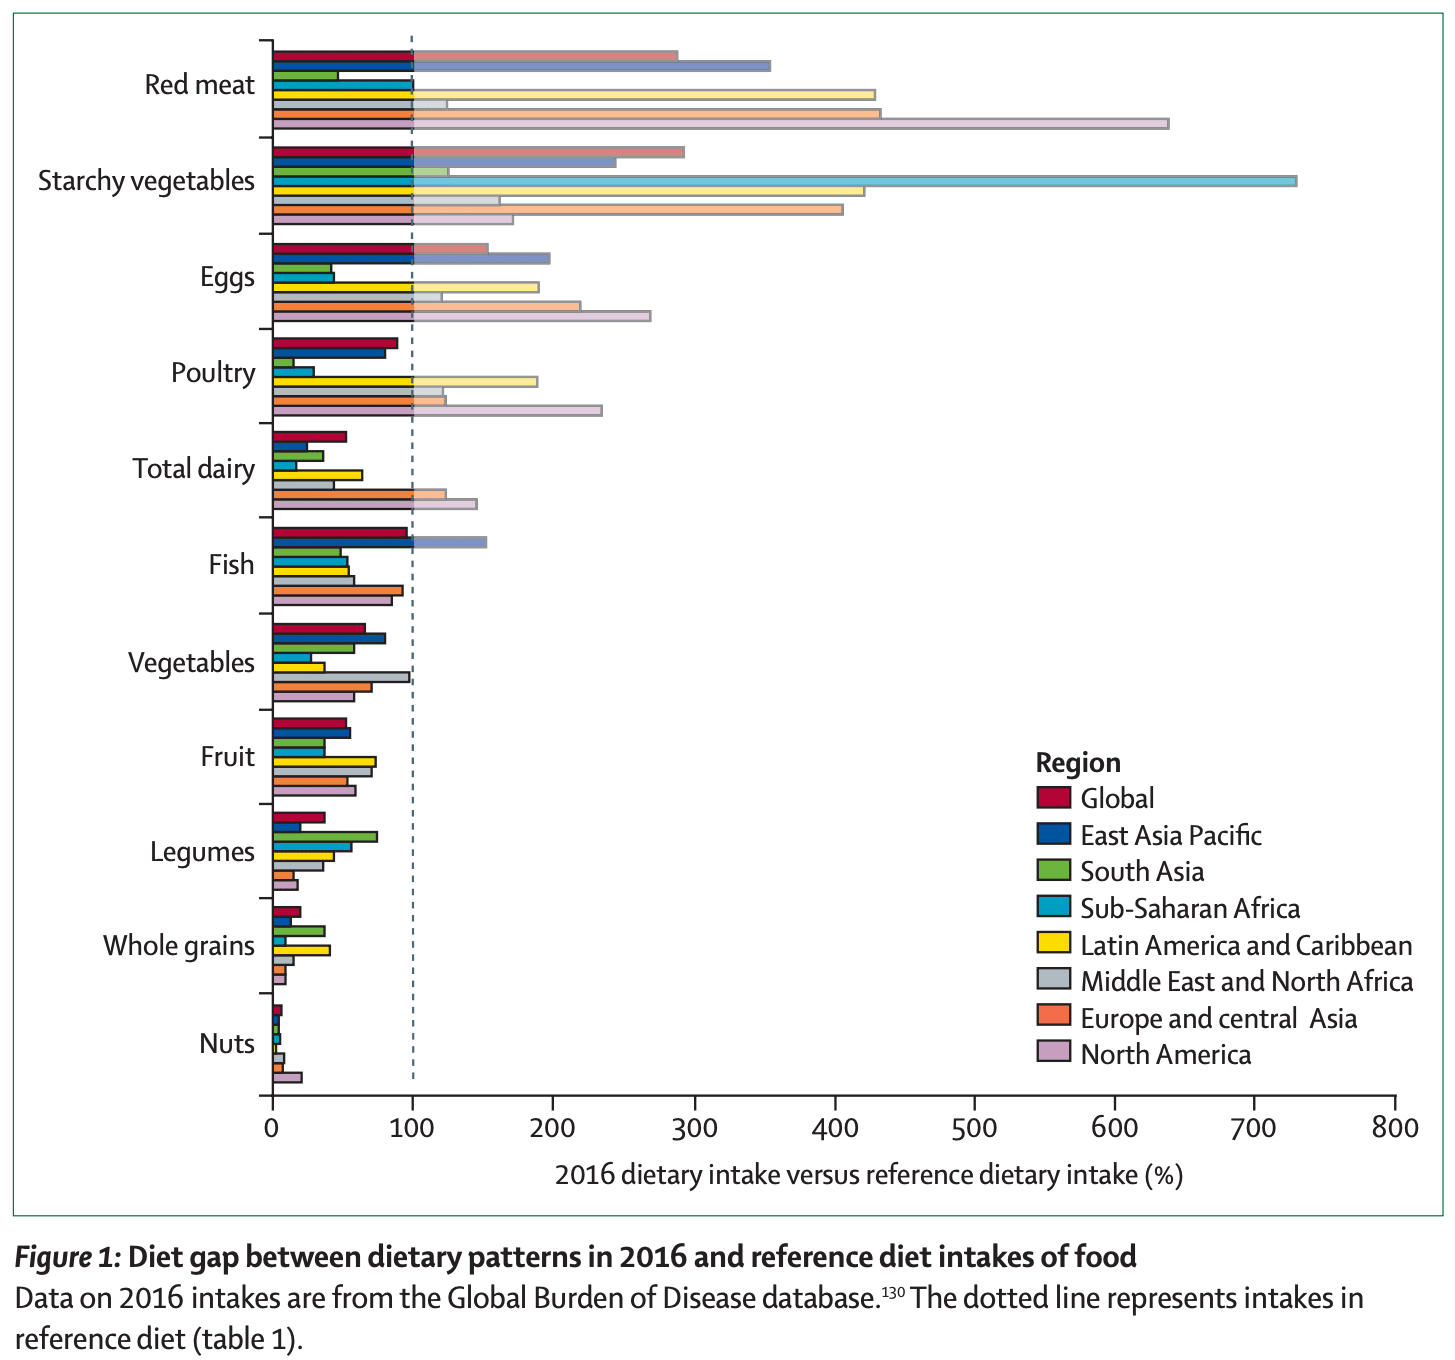
\includegraphics[width=17cm]{images/Libro-img023.png}
    \caption{Sull'asse Y, leggendo dall'alto verso il basso troviamo, carne rossa, verdure
amidacee, uova, pollame, latticini, pesce, vegetali, frutta, legum, cereali integrali, noccioline. 
Nella legenda troviamo: Globale, Asia dell'est, Sud Asia, Africa subsahariana, America latina e Caraibi, nord Africa e Medio Oriente, Europa e Asia centrale, nord America }
  \end{minipage}
\end{figure}

Alcuni studi infine sostengono che l'uomo abbia iniziato uno stato di adattamento a diventare onnivoro iniziato durante
il periodo delle glaciazioni circa 2 milioni di anni fa. In quanto primati abbiamo tante caratteristiche da erbivori.
Tutt'ora condividiamo il 98\% di DNA con le grandi scimmie, chiamate anche ominidi, che sono gorilla, scimpanzé, bonobo
e orango e, alla quale apparteniamo anche noi homo sapiens. 

Le \ caratteristiche che ci rendono più simili agli erbivori sono:

\begin{itemize}
\item ridotta apertura della bocca
\item denti incisivi larghi e piatti con canini corti e smussati
\item unghie piatte
\item lunga masticazione
\item l'intestino tenue dei carnivori è lungo da 3 a 6 volte la lunghezza del corpo, negli erbivori da 10 a 12 (11
nell'uomo)
\item anche la saliva, il fegato, reni e altri organi sono più simili a quelli degli erbivori
\end{itemize}

\bigskip

Se non volete rinunciare alla carne abbiamo comunque diverse strategie:

\begin{itemize}
\item Ridurre il consumo di carne: come abbiamo visto noi occidentali ne mangiamo troppa, sia per
l'ambiente, che per la nostra salute a circa due porzioni a settimana.
\item Mangiare gli “scarti” di lavorazione: Si dice che del maiale non si butti via niente, ed è proprio così, ma
purtroppo nell'industria alimentare vengono sprecate molte porti
dell'animale, anche e soprattutto dei bovini. Potete informarvi da qualche allevatore locale e,
mangiare quello che di buono viene scartato durante la lavorazione ed essere più efficienti, il vostro impatto
ambientale sarebbe zero.
\item Mangiare gli “invasori”: Ci sono alcune specie aliene, nel senso che non sono originarie di un certo luogo, come
per esempio la nutria o il pesce siluro qua in Italia, che sono stati importati da altri paesi. Queste specie, non
trovando predatori naturali hanno si stanno moltiplicando, diventando un problema per altre specie animali, vegetali e
per l'ecosistema in generale. Se conosciamo un cacciatore o chiedendo in comune di presentarcene
uno e, se l'animale è commestibile e buono, possiamo chiedere di tenercene da parte qualcuno per
poi mangiarcelo. Ora gli animalisti probabilmente non saranno d'accordo con me. Sicuramente
quell'animale merita di vivere, soffre come tutti noi e non ha scelto lui di trovarsi come specie
invasiva. Ma purtroppo è successo. Dobbiamo fare in modo che non succeda più ma intanto contenere il problema. Dal
punto di vista emotivo anche una sola morte è troppa. Ma dal punto di vista oggettivo e distaccato, la vita di questi
animali comporta la morte di molti più animali. Mi rendo conto sia una scelta triste, ma proprio perché amiamo gli
animali e la biodiversità dobbiamo farlo. Morirebbero molti più animali se si lasciassero in vita le specie aliene.
Ricordo anche che le specie aliene o invasive sono sia animali che vegetali. Per saperne di più potete visitare
eattheinvaders.org
\end{itemize}

\bigskip

\clearpage\subsection{Reducetariani e flexitariani}
Un sondaggio condotto nel
2012\endnote{\protect\url{https://www.ted.com/talks/brian\_kateman\_how\_to\_reduce\_your\_diet\_s\_carbon\_footprint\_without\_going\_vegan?language=it}
} ha scoperto che i vegetariani sono circa il 5\% e questa percentuale non cambia dal 1999. Questo perché tra le
\ persone che si definiscono vegetariane, circa 2/3 hanno dichiarato di aver mangiato carne di recente. La maggioranza
dei vegetariani non è quindi “integralista” e, questo può dipendere da diversi fattori, potrebbe essere in una fase di
transizione, vuole impattare meno sull'ambiente ma non essendo un nutrizionista ci va cauto per la
saluto, o magari quando è ospite a casa di qualcuno non vuole che gli si prepari cibo a parte o per mille altre
ragioni, ma comunque ci tiene a mostrare nella sua identità un'attenzione al cambiamento
climatico, definendosi così vegetariano, anche se qualche volta all'anno o al mese mangia carne. Anche perché come
abbiamo visto, esistono tante tipologie, quindi presentarsi come un \ Latto-ovo-pesce-vegetariano a uno che abbiamo
conosciuto potrebbe dover essere seguito da una spiegazione che, come prima impressione, ci farebbe passare subito come
dei boriosi. A complicare o forse a semplificare le cose esistono due nuovi termini: Reducetariani e flexitariani, ma
chi sono? Entrambi si impegnano a ridurre il consumo di carne, i primi per l'ambiente e i secondi
per la propria salute. La maggioranza dei vegetariani sono quindi reducetariani o flexitariani. 


\bigskip
\begin{mdframed}[linewidth=1pt]
Anche l'attuale eccesso di cibi processati, di igiene, di farmaci, soprattutto antibiotici, assunti
direttamente o indirettamente tramite animali contribuiscono a danneggiare un'utile popolazione
del nostro intestino, ilmicrobiota. Un microbiota indebolito da un ambiente eccessivamente pulito e
dall'utilizzo massivo di antibiotici potrebbe essere una delle cause della grande diffusione di
allergie degli ultimi decenni. La letteratura evidenzia infatti come il nostro sistema immunitario diventi davvero
efficiente soltanto se fin dalla nascita si viene a contatto con una quantità sufficiente di germi e parassiti. 
\end{mdframed}

\bigskip

Forse questa può essere strada del cambiamento attraverso questo stile di vita. Purtroppo per anni, la promozione del
messaggio vegetariano e vegano ha fatto leva sul: voi siete sbagliati e dovreste vergognarvi mentre noi siamo buoni e,
ora quando uno si definisce vegetariano, in misura più o meno grande, crea un po' di imbarazzo negli altri, anche se
spiegamo che non è nostra intenzione giudicare cosa gli alti mangiano. Con il termine reducetariano rimuoviamo questo
linea così netta tra un gruppo e l'altro, risultando più inclusivo. Talmente inclusivo che tutti
possiamo diventare reducetariani. Se tutti noi seguissimo una dieta del “lunedì senza carne”, astenendoci dal mangiare
carne ogni lunedì, avremmo un miliardo di vegetariani in più dall'oggi al domani. Penso che tutti possano avere piacere
ed essere gratificati dall'aver fatto la differenza con una piccola rinuncia.

\clearpage\subsection{Cosa si può fare?}

\begin{wrapfigure}{i}{9cm}
  \centering
  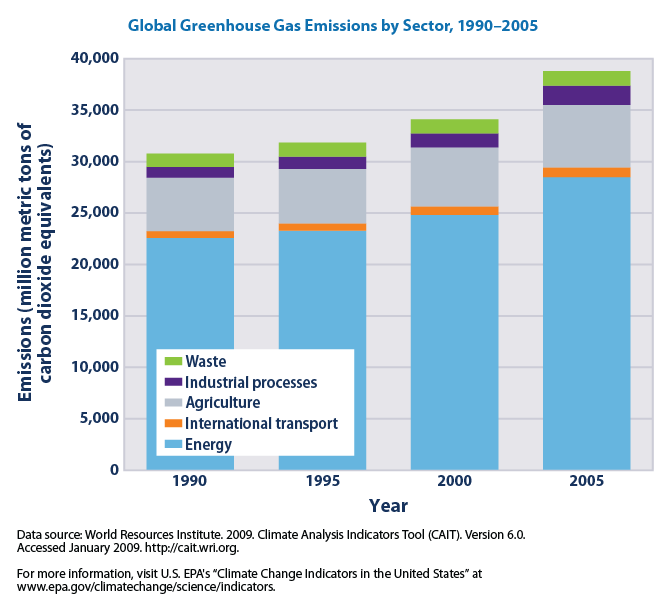
\includegraphics[width=0.95\linewidth]{images/Libro-img024.png}
  \begin{minipage}{\linewidth}
    \caption{Legenda tradotta: Rifiuti, processi industriali,
agricoltura, trasporti internazionali e energia. 
Credits: By US Environmental Protection Agency - Climate Change Indicators in the United States: Figure 2. Global
Greenhouse Gas Emissions by Sector, 1990-2005. Page 12 of PDF. Published 2010., Public Domain,
\protect\url{https://commons.wikimedia.org/w/index.php?curid=20445607} }
  \end{minipage}
\end{wrapfigure}

Per riuscire in questa sfida ecologica siamo chiamati a fare dei cambiamenti individuali, come abbiamo visto in queste
pagine, come l'alimentazione, riciclare, prestare attenzione ai modi che utilizziamo per spostarci
ecc… Le scelte importanti che possono abbassare il nostro impatto ambientale non comportano una riduzione del tenore di
vita, ma un cambiamento. L'importanza di queste scelte non vanno viste soltanto per preservare il
pianeta del futuro, di quando non ci saremo più, ma anche per quello attuale. In Europa un decesso su otto è dovuto
all'inquinamento\endnote{\protect\url{https://www.wired.it/attualita/ambiente/2020/09/09/europa-decessi-inquinamento/}
\ }. A volte può risultare difficile fare cambiamenti che possano ridurre le proprie emissioni, ma possiamo
riassorbirle. Ci sono siti come Treedom, ZeroCO2 e Ecosia che tra le varie cose permettono, di farti piantare alberi in
giro per il mondo. Alcune teorie infatti spiegano che sia più semplice riassorbire che ridurre i gas serra. Inoltre
dobbiamo cambiare anche l'organizzazione della società a livello mondiale, infatti come scritto su
The Guardian, 100 aziende sono responsabili del 71\% dell'inquinamento
mondiale\endnote{\protect\url{https://www.wired.it/scienza/energia/2021/07/27/inquinamento-centrali-elettriche-emissioni/} }, qua
potete trovare i nomi di queste
società\endnote{\protect\url{https://www.theguardian.com/sustainable-business/2017/jul/10/100-fossil-fuel-companies-investors-responsible-71-global-emissions-cdp-study-climate-change}
}. Cosa producono queste aziende? Principalmente energia bruciando combustibili fossili, carbone, petrolio. La
produzione di energia è infatti il settore principalmente responsabile nell'emissione di gas
serra, come possiamo vedere nel grafico qui a fianco.

\begin{figure}[H]
  \centering
  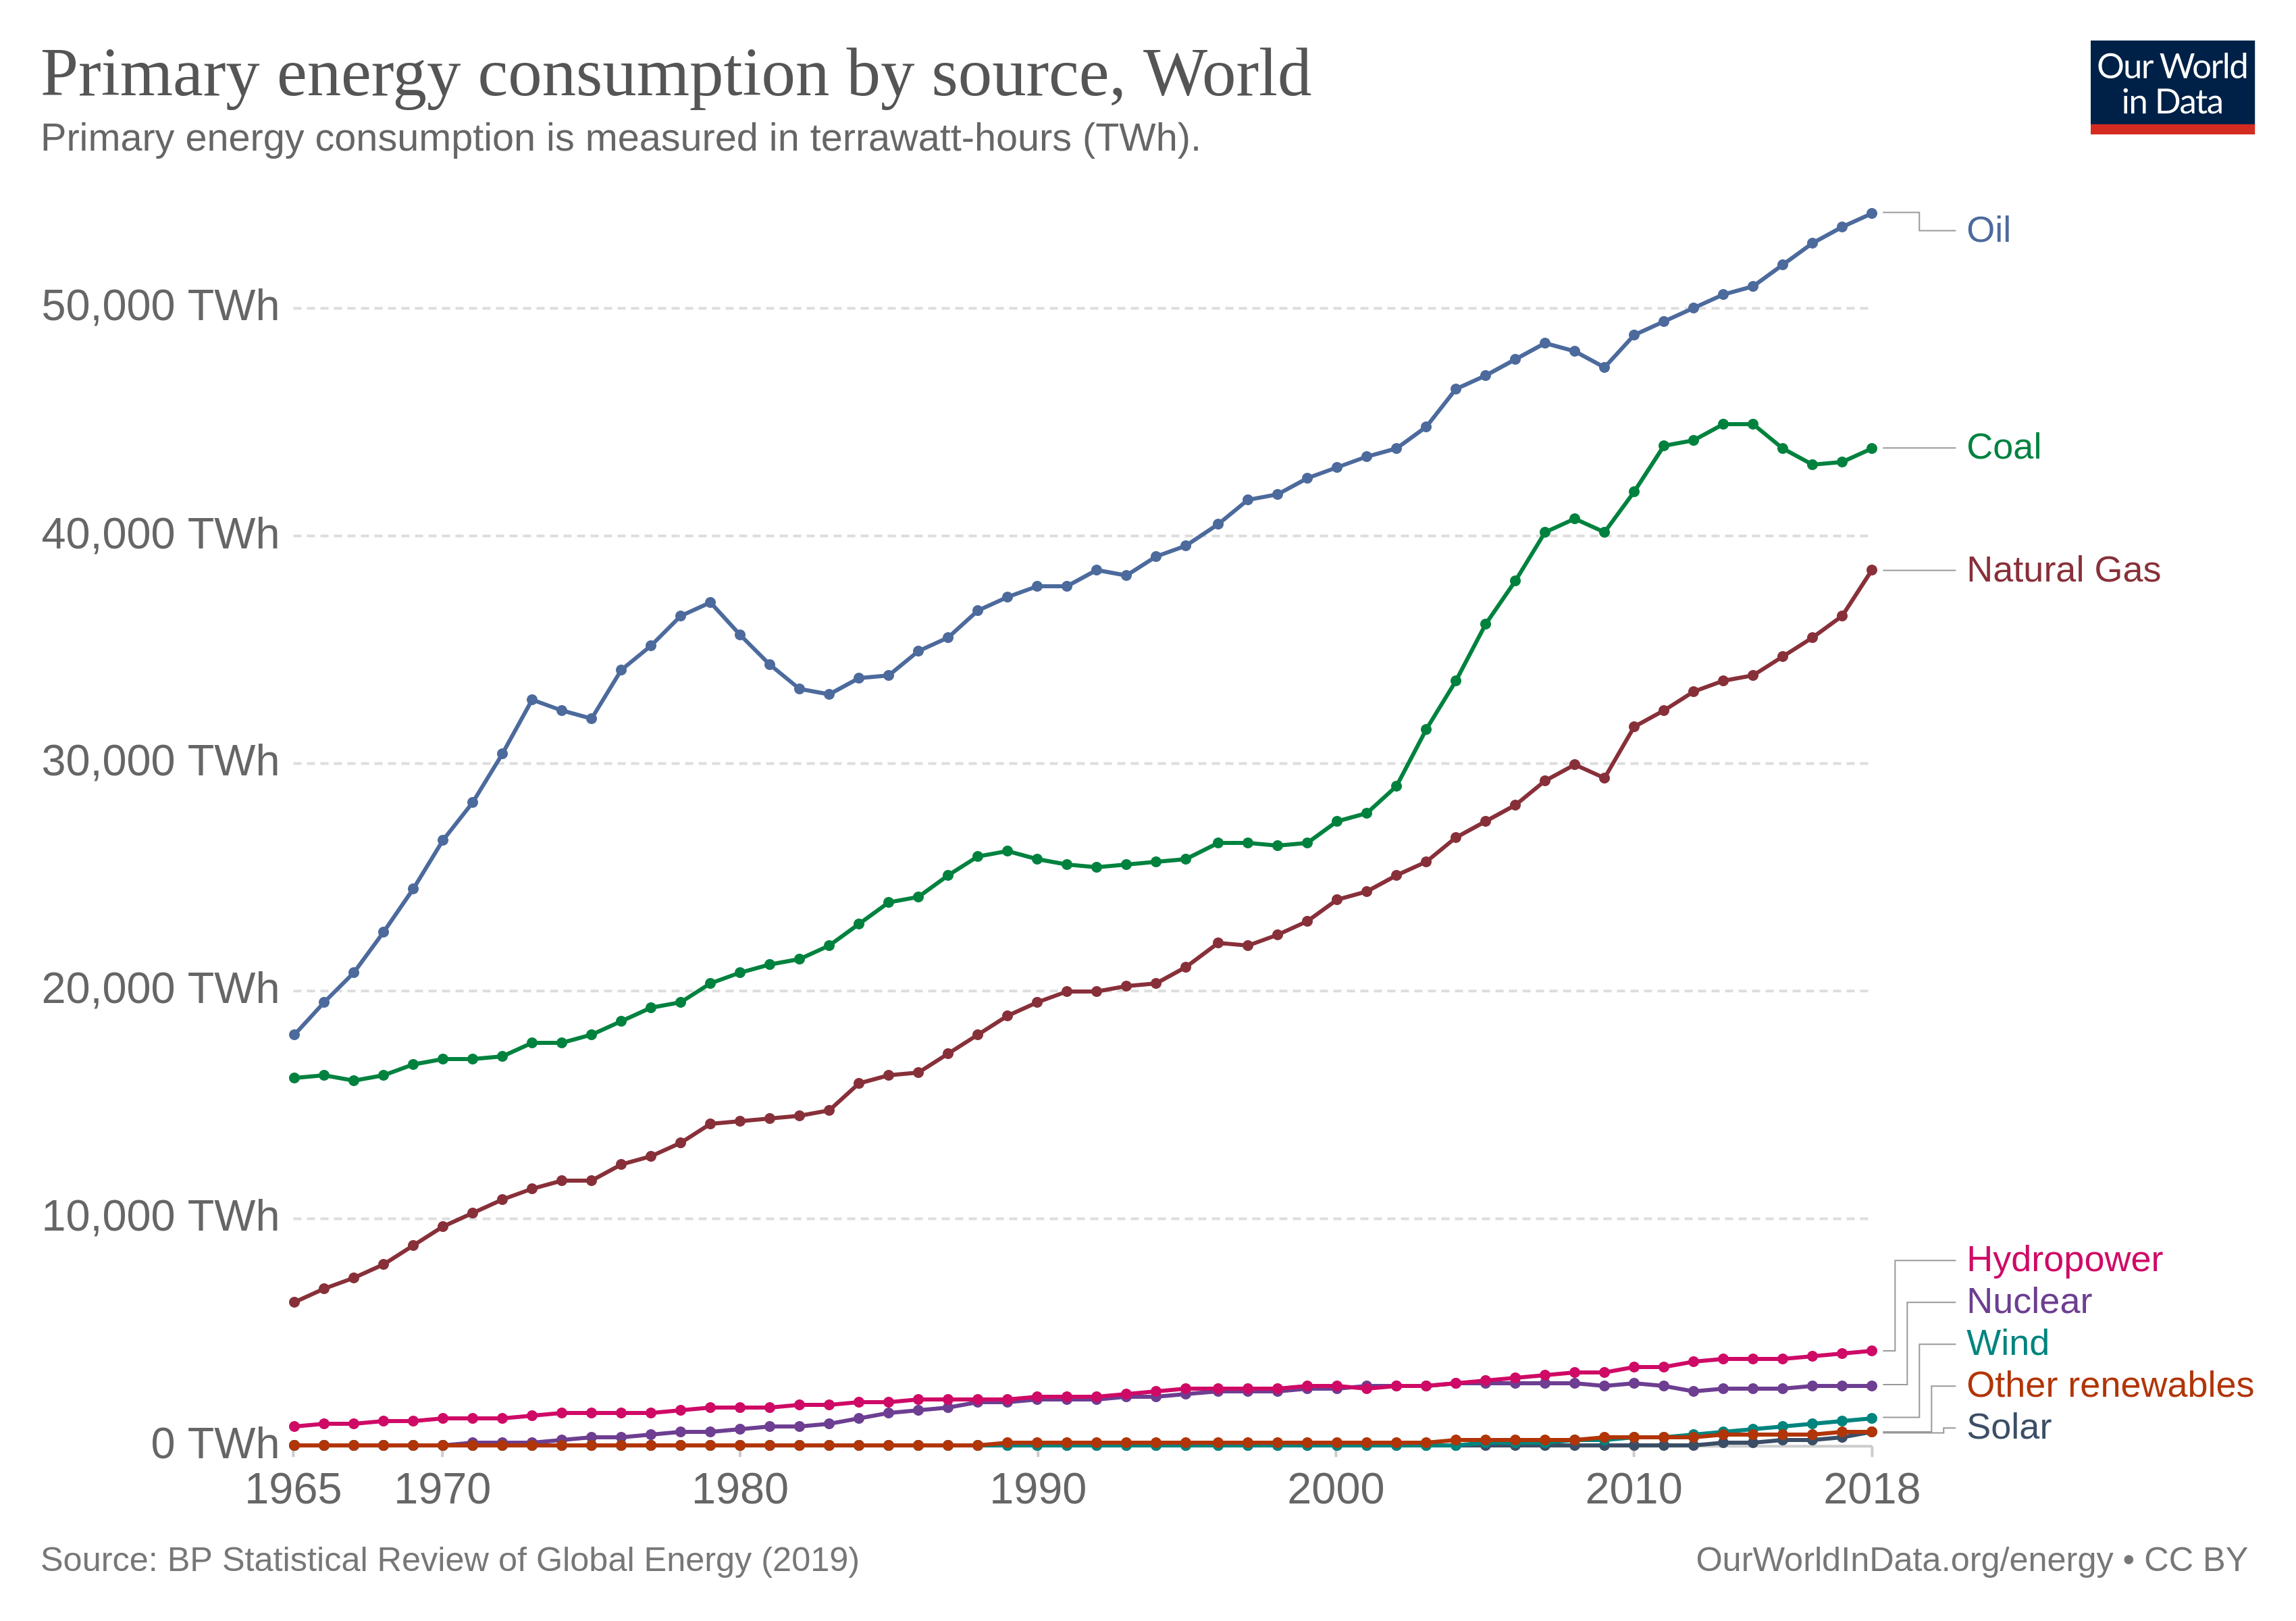
\includegraphics[width=0.95\linewidth]{images/Libro-img025.png}
  \caption{Dall'alto verso il basso: Petrolio, carbone, gas naturale, idroelettrico, nucleare, eolico, altro e solare
  Credits: \protect\url{https://ourworldindata.org/energy} }
\end{figure}

Seppur l'impiego di carbone, petrolio e gas naturali per la produzione energetica non siano più
metodi all'avanguardia, sono ancora molto diffusi. Potremmo essere portati a pensare che comprando
una macchina elettrica e scaldando casa con l'elettricità il grosso
dell'energia che utilizzeremo sarà pulita. Non proprio! Dipende da come viene prodotta la
corrente, infatti ad oggi, l'energia elettrica viene prodotta principalmente da carbone e gas
naturale. Nel grafico a torta qui a fianco possiamo vedere la situazione mondiale, ma anche in Italia, come riportato
dal Wwf\endnote{\protect\url{https://www.wwf.it/il\_pianeta/clima\_ed\_energia/fermiamo\_il\_carbone/} }
l'11,6\% della produzione elettrica deriva dal carbone mentre troppe centrali termoelettriche
lavorano per un terzo della loro potenzialità. In Italia possiamo generare una potenza doppia al picco massimo mai
raggiunto, per cui potremmo chiudere o convertire in centrali green tutte quelle più inquinanti. Quindi scegliere di
scaldare casa con una pompa di calore e comprare una macchina elettrica è sicuramente una buona idea se il vostro
fornitore di corrente la produce tramite fonti rinnovabili. Questo è un esempio di scelta che non cambia il nostro
tenore di vita, basta fare una telefonata al vostro fornitore di elettricità e chiedere in che percentuale vengono
utilizzate nella produzione fonti rinnovabili e non. A volte non è nemmeno necessario cambiare fornitore, ma solo
contratto. Anche in Italia abbiamo fornitori che producono corrente al 100\% da fonti rinnovabili e il prezzo è lo
stesso di fornitori che utilizzano combustibili fossili. Io quando ho cambiato fornitore per passare a corrente
prodotta da fonti rinnovabili addirittura ho risparmiato rispetto al precedente contratto non completamente green.

\begin{figure}[H]
  \centering
  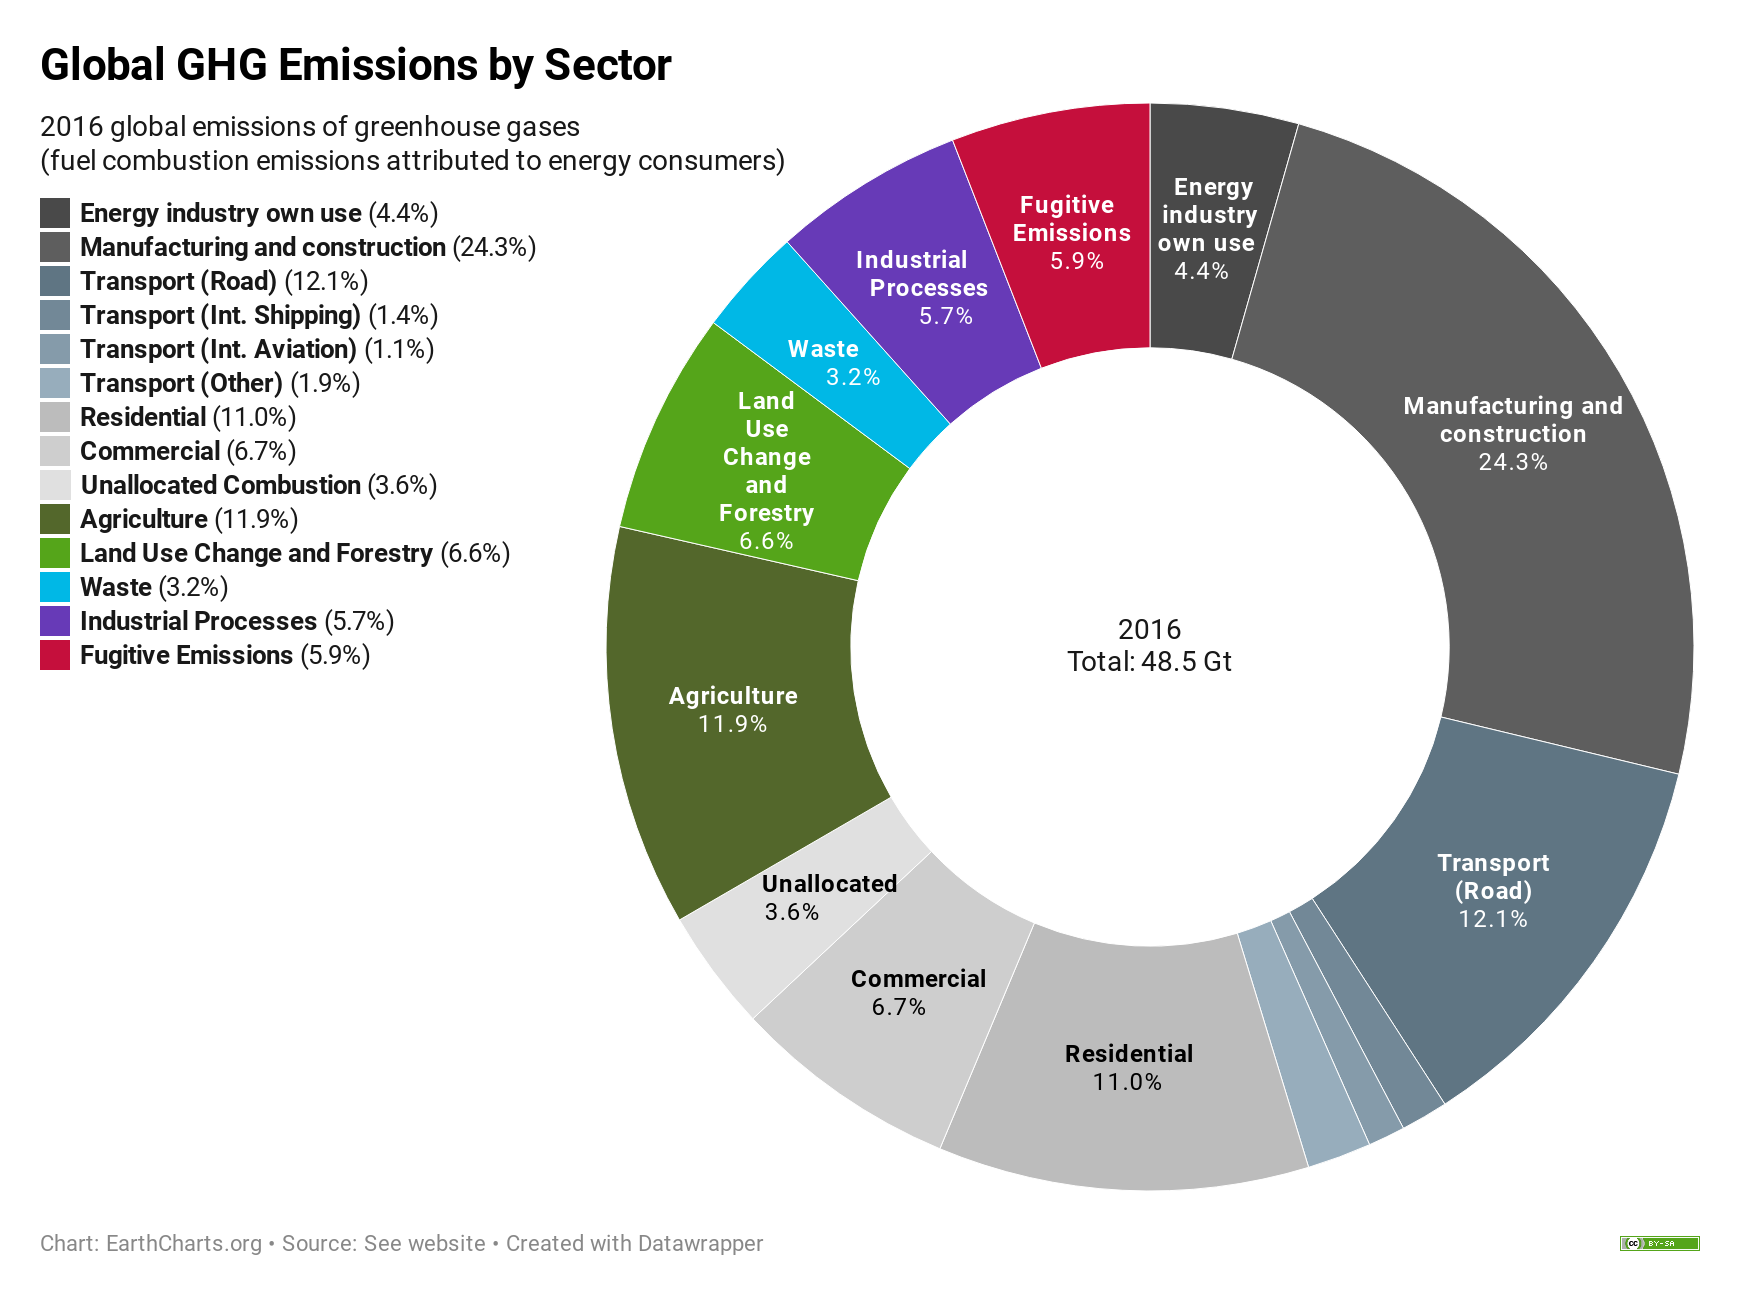
\includegraphics[width=0.95\linewidth]{images/Libro-img026.png}
  \caption{Grafico con le emissioni globali di gas serra del 2016 per settore. 
Credits: By Simon Rayner / EarthCharts - EarthCharts Website (\protect\url{http://earthcharts.org/),}
\protect\url{http://earthcharts.org/wp-content/uploads/2020/03/Emissions-Sources.png,} CC BY-SA 4.0,
\protect\url{https://commons.wikimedia.org/w/index.php?curid=87783234}}
\end{figure}

Quindi è vero che ci sono 100 aziende che sono responsabili del 71\% dell'inquinamento, quindi
anche con lo sforzo della collettività e l'ottimizzazione dei nostri consumi, nella nostra vita
privata, possiamo andare a lavorare solo su una percentuale minore del restante 29\%. O forse no? Le aziende rispondono
in funzione della legge economica della domanda e dell'offerta, se le industrie e i privati
cittadini acquistassero energia solo da chi la produce in maniera pulita, queste 100 aziende, dovrebbero chiudere o
meglio ancora convertirsi in produzione green. E questo vale un po' per tutto. Se noi consumatori
spendiamo i nostri soldi per beni e servizi prodotti in maniera etica, possiamo cambiare il mondo. La tendenza, sia nel
privato che nelle aziende è sicuramente positiva, infatti l'impiego di energie prodotte da fonti
rinnovabili è sempre maggiore di anno in anno, a discapito dei combustibili fossili. Ma siamo ancora troppo lenti. Gli
esperti hanno stimato che tra il 2030 e il 2050 la terra potrebbe diventare troppo inospitale per la vita umana, per
cui dobbiamo accelerare i tempi di questo cambiamento già in atto e possibile già oggi. Noi nel nostro piccolo, da
soli, possiamo solo cambiare il nostro stile di vita, necessario ma non sufficiente, per poter produrre un cambiamento
su scala globale dobbiamo unirci e, la rete ci viene incontro.

Diversi enti stanno facendo proprio questo, chiamare persone all'azione attraverso eventi,
manifestazioni, petizioni ecc… Potete rimanere informati sugli eventi attraverso i siti o le pagine social, tra i più
importanti possiamo trovare:

greenpeace.org/italy

wwf.it

footprintnetwork.org

fridaysforfutureitalia.it 


\bigskip

E siti di petizioni online:

avaaz.org

wemove.eu

change.org


\bigskip

Potete trovare ulteriori informazioni e grafici su
Wikipedia\endnote{\protect\url{https://en.wikipedia.org/wiki/World\_energy\_consumption} }
\endnote{\protect\url{https://en.wikipedia.org/wiki/Greenhouse\_gas} }.


\bigskip

Noi italiani siamo abbastanza esterofili e, su tanti aspetti abbiamo ragione di esserlo. Ma ci sono cose, davvero
importanti di cui dobbiamo essere orgogliosi. Abbiamo un ottimo sistema sanitario e in generale tutto il
welfare\endnote{\protect\url{https://en.wikipedia.org/wiki/List\_of\_countries\_by\_social\_welfare\_spending} }, ammortizzatori
sociali, malattia, maternità, ferie ecc… Inoltre tra i paesi più industrializzati siamo quello che consuma meno energia
e sta investendo molte risorse nella conversione verso fonti rinnovabili.

\begin{figure}[H]
  \centering
  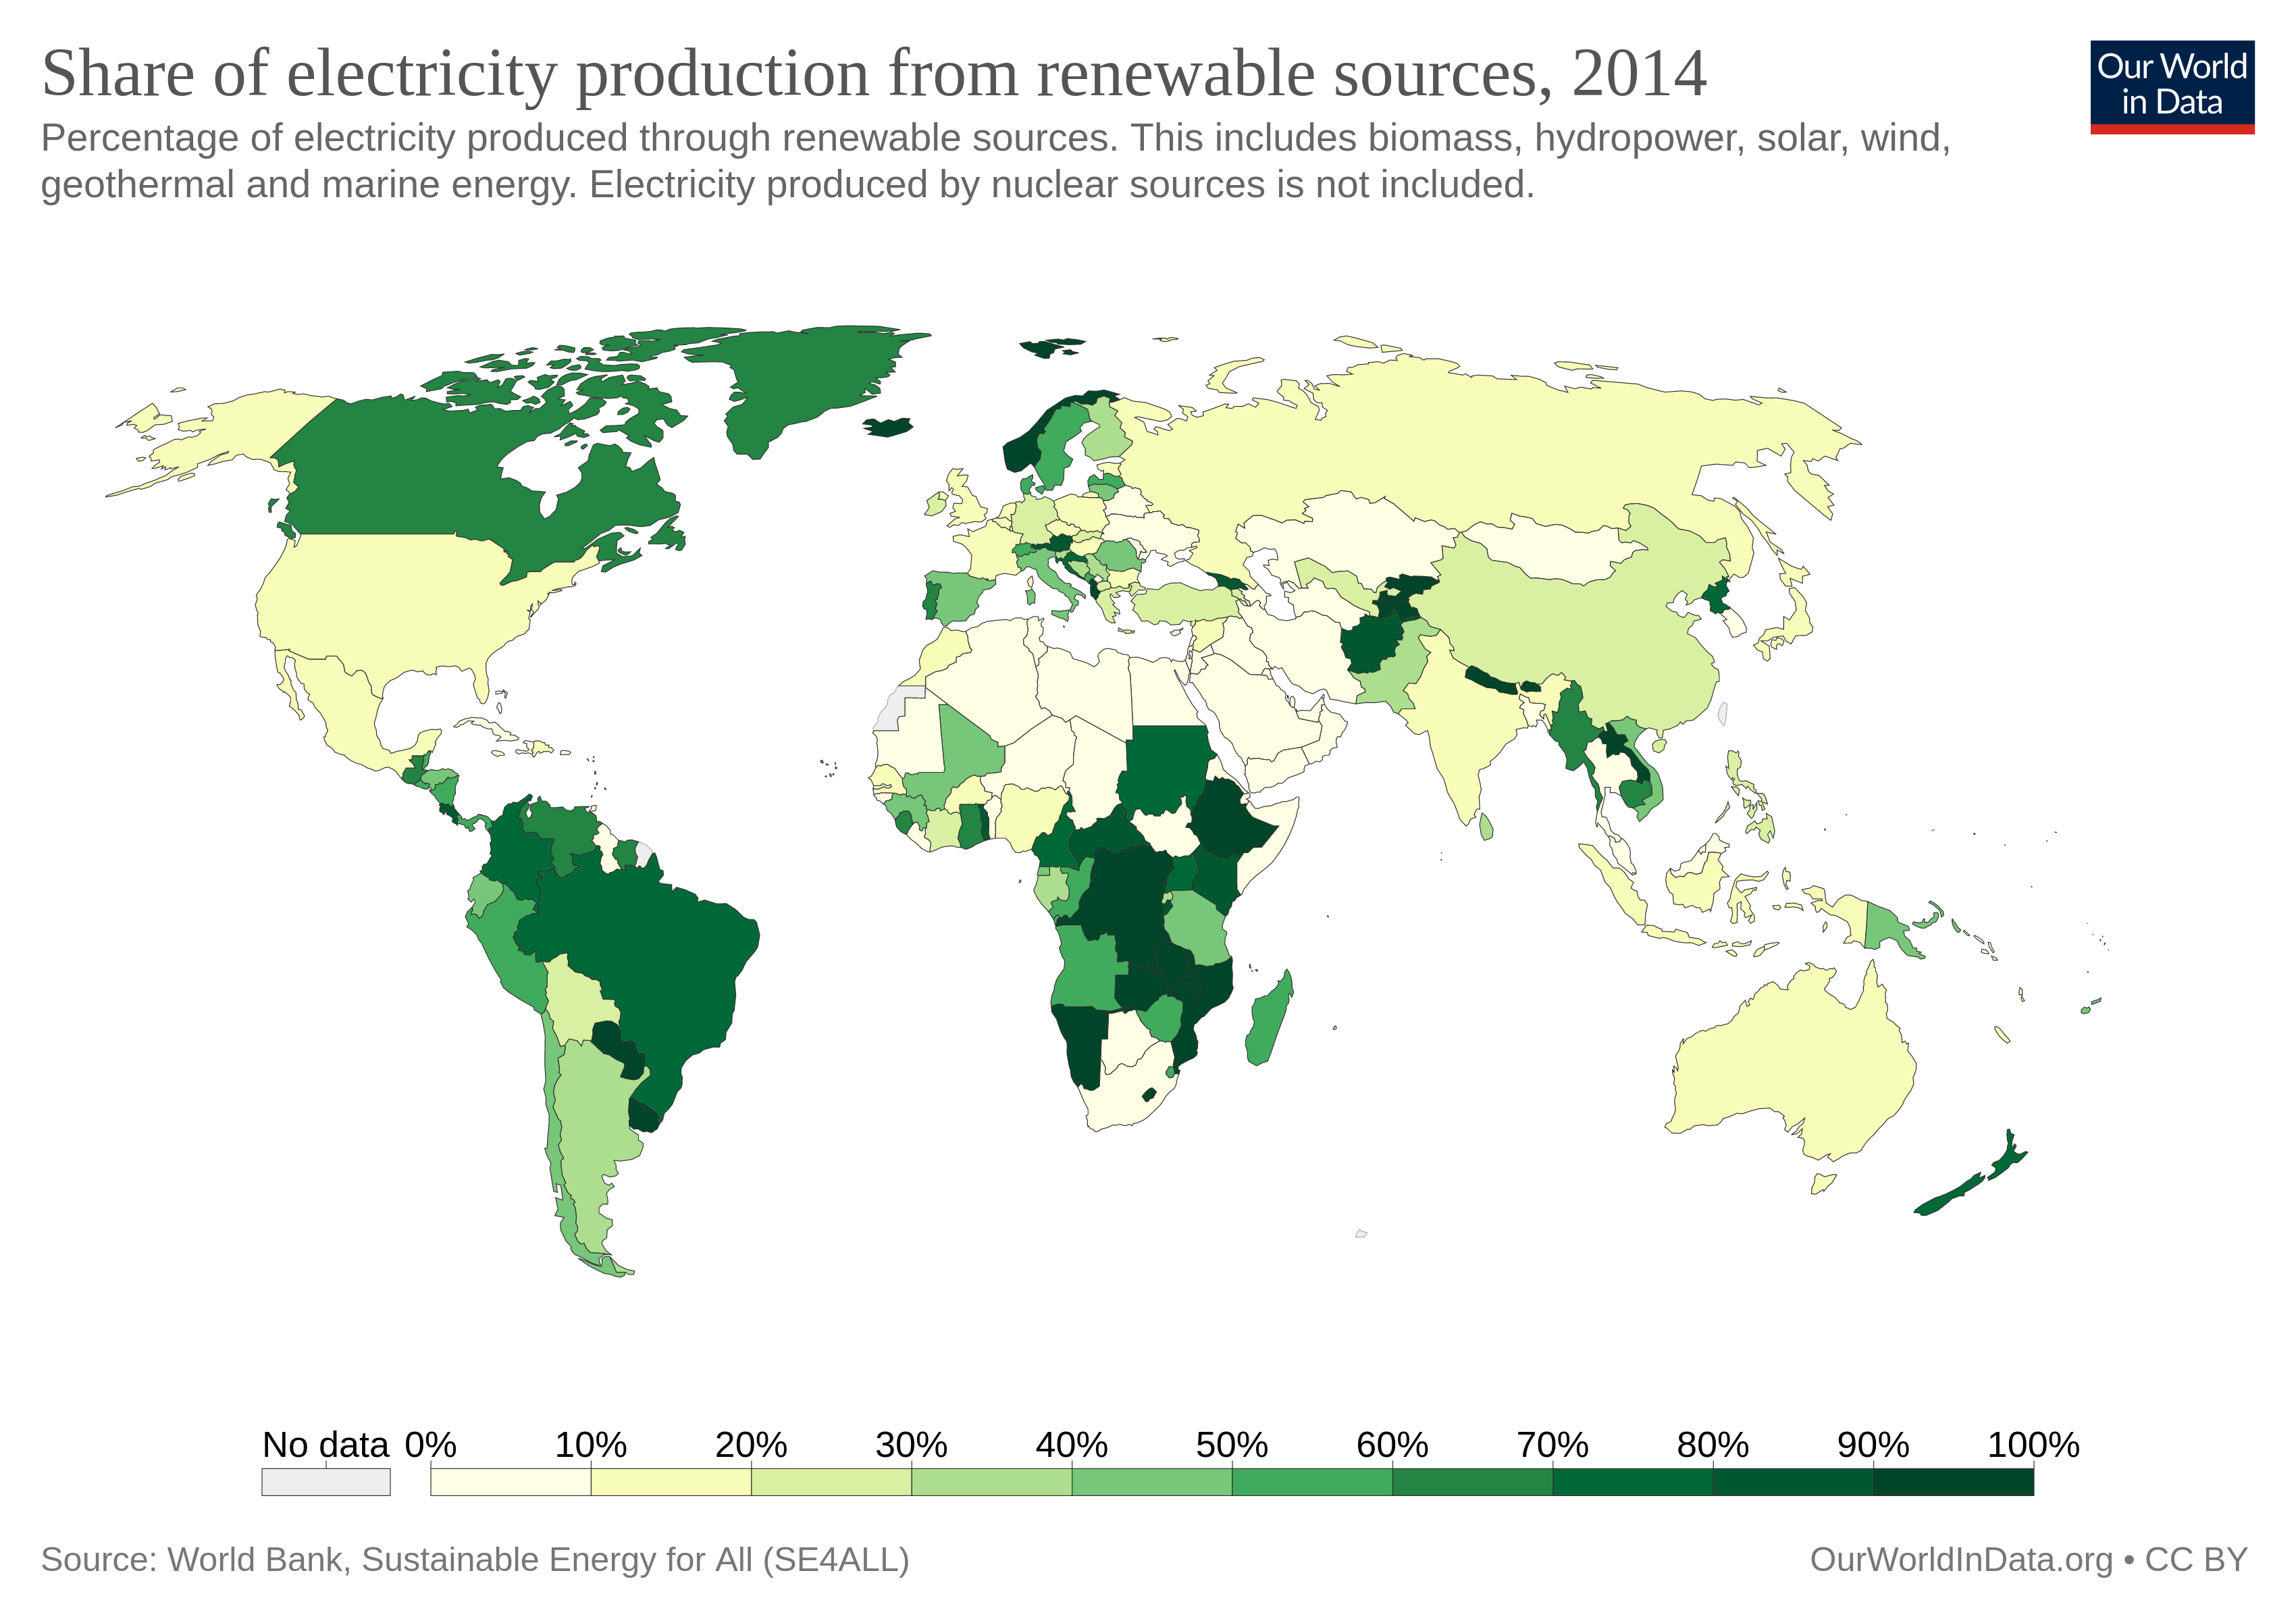
\includegraphics[width=0.95\linewidth]{images/Libro-img027.png}
  \caption{Percentuale di elettricità prodotta attraverso fonti rinnovabili nel 2014. 
Credits: \protect\url{https://ourworldindata.org/energy}}
\end{figure}

\bigskip

Si potrebbero sollevare delle critiche sull'Italia, come il fatto che ci sia una forte pressione
fiscale, ma come possiamo vedere nelle mappe qui di seguito, welfare e tasse vanno abbastanza di pari passo anche per
gli altri paesi europei. Questo non ci deve portare al nazionalismo più cieco, l'Italia ha anche
una pressione fiscale alta perché è il paese che più di tutti evade il fisco, più numerosi altri problemi che ci
portano ad essere il fanalino di coda dell'occidente, come ad esempio
l'occupazione.

\begin{table}[H]
\centering
\caption{Possiamo notare una correlazione tra tasse e welfare. Le mappe sono focalizzate solo sull'Europa in quanto nel resto del mondo non si hanno dati, come potete constatare entrando nella fonte. Inoltre la testa della classifica è composta da stati europei: 1° Francia, 2° Finlandia 3° Belgio 4° Italia, 5° Danimarca, il Giappone si trova in 11° posizione, Nuova Zelanda 21° e Stati Uniti al 23.}
\begin{tabular}{cc}
  \begin{subfigure}{0.5\textwidth}
    \centering
    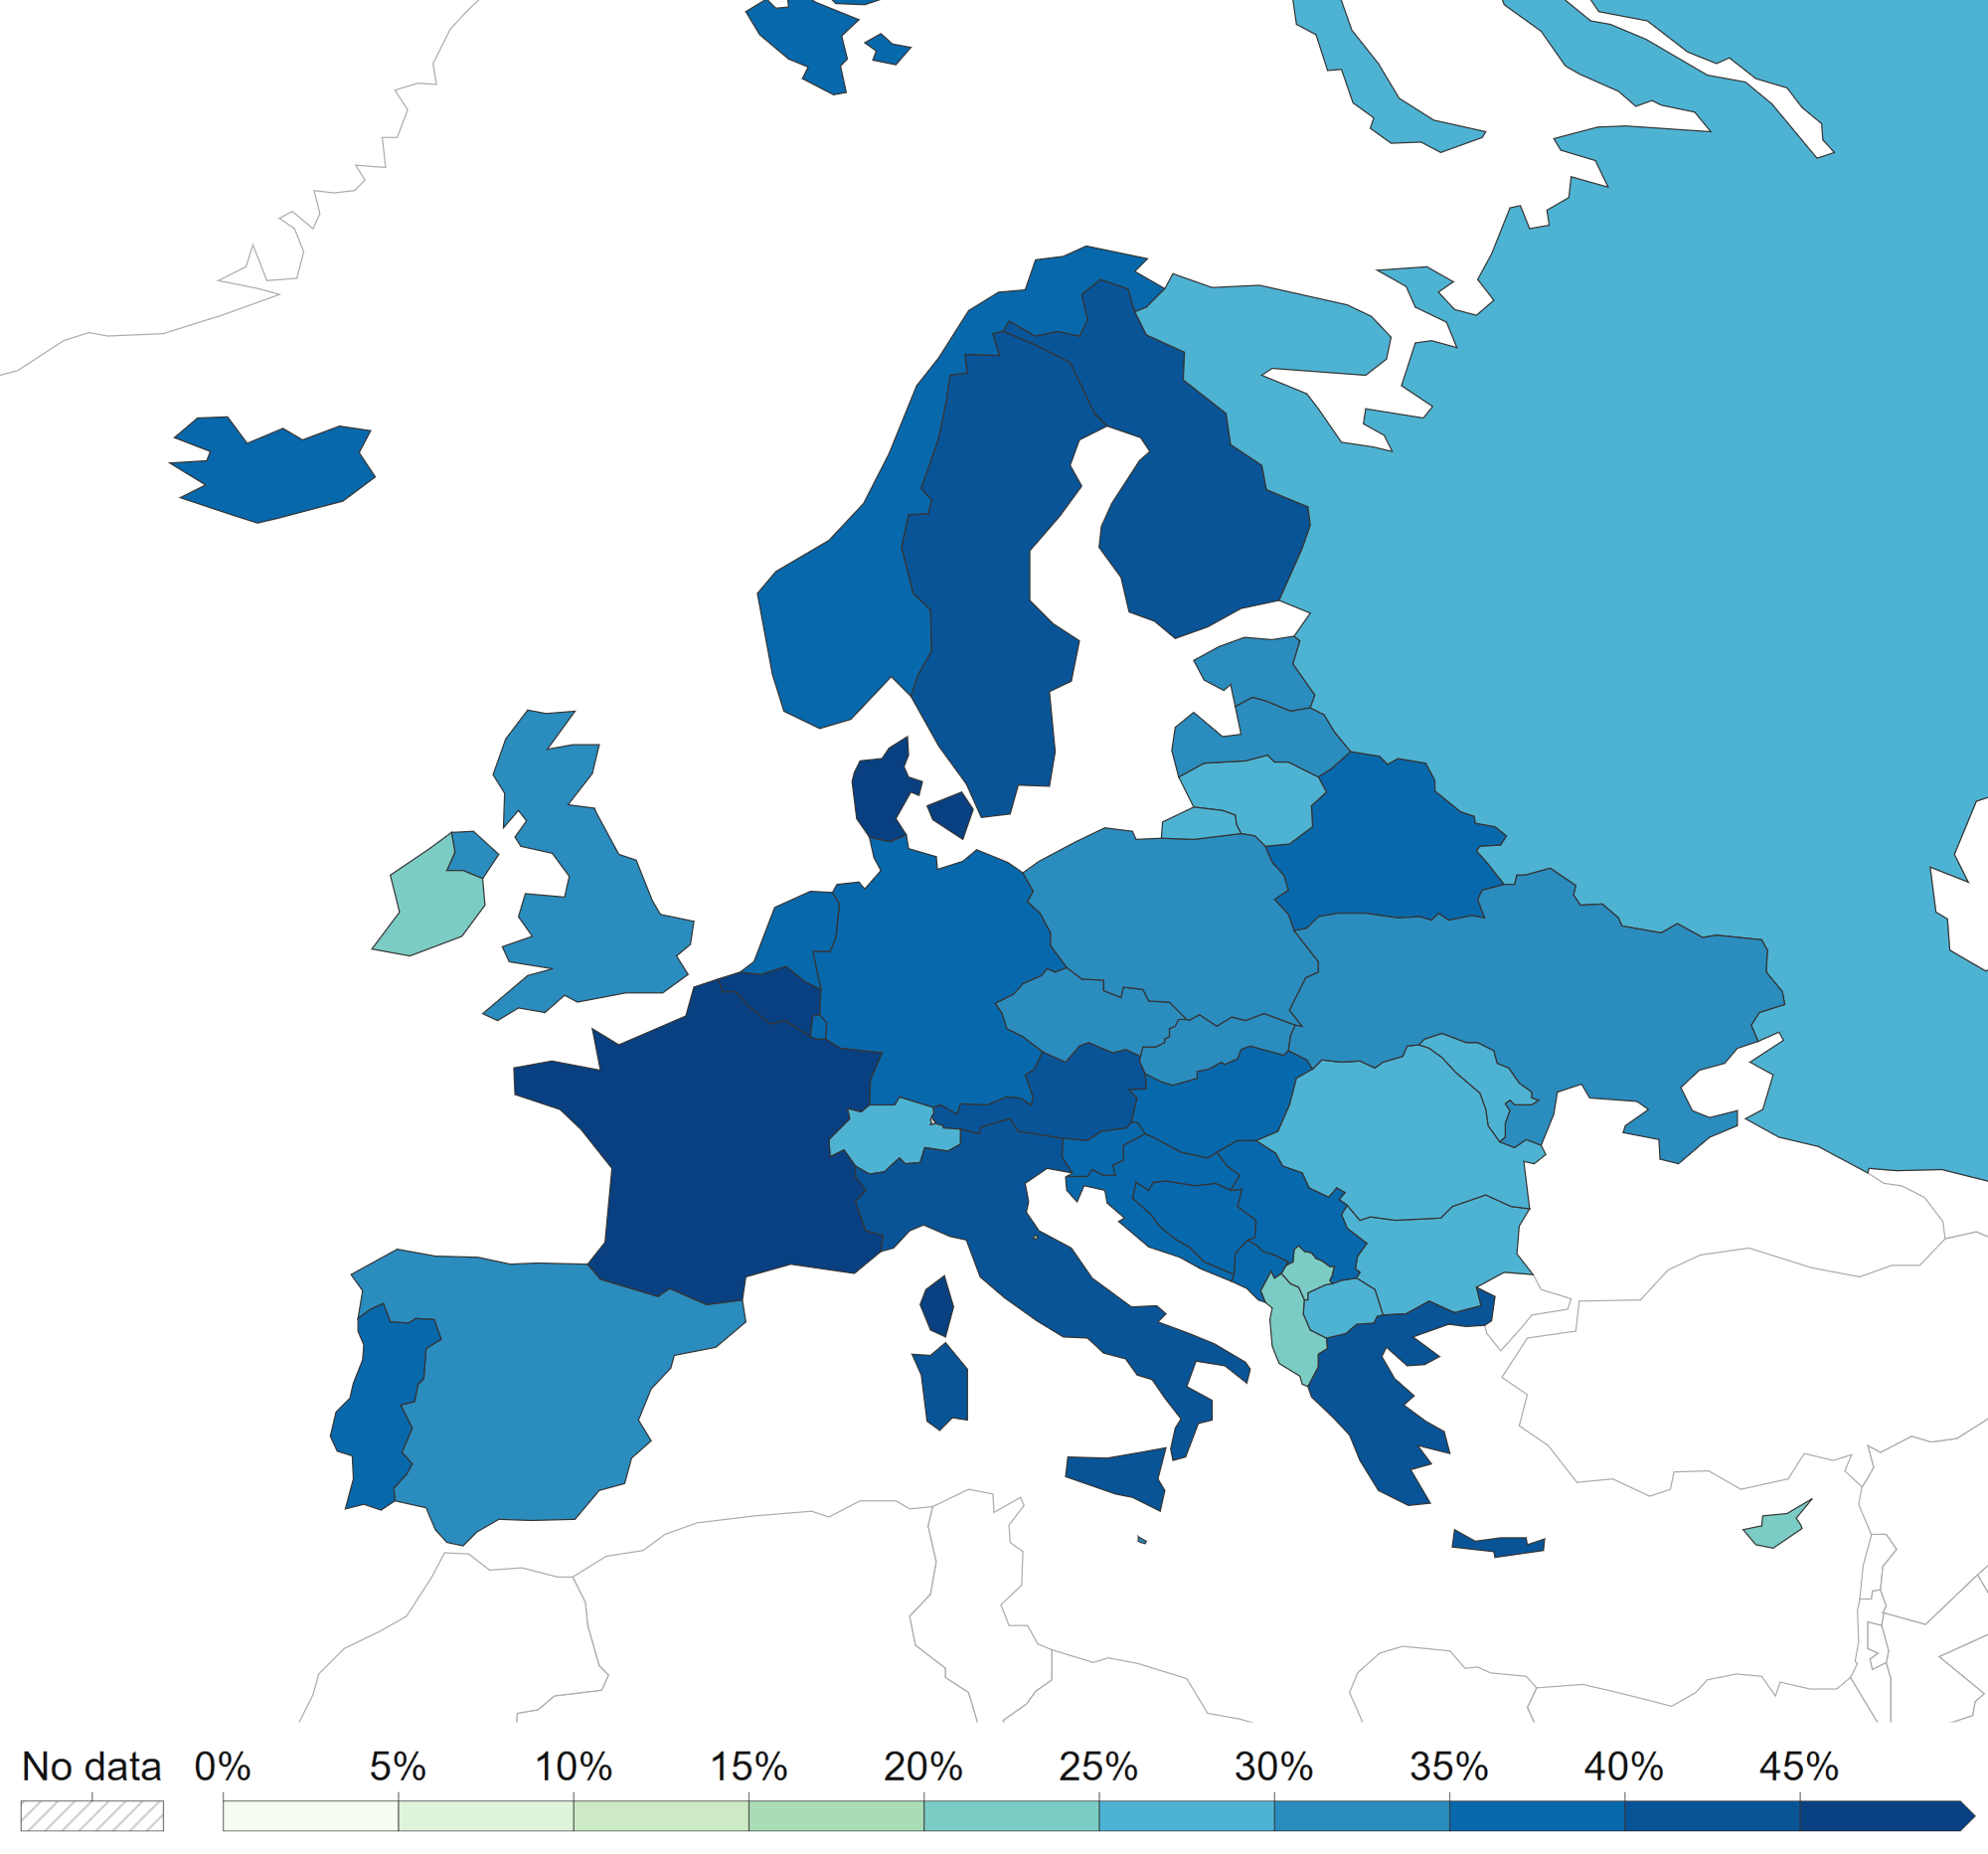
\includegraphics[width=0.8\linewidth]{images/Libro-img028.png}
    \caption{Entrate fiscali totali, 2016 - Fonte: \protect\url{https://ourworldindata.org/grapher/total-tax-revenues-gdp?tab=map\&time=2016}}
  \end{subfigure}
  &
  \begin{subfigure}{0.5\textwidth}
    \centering
    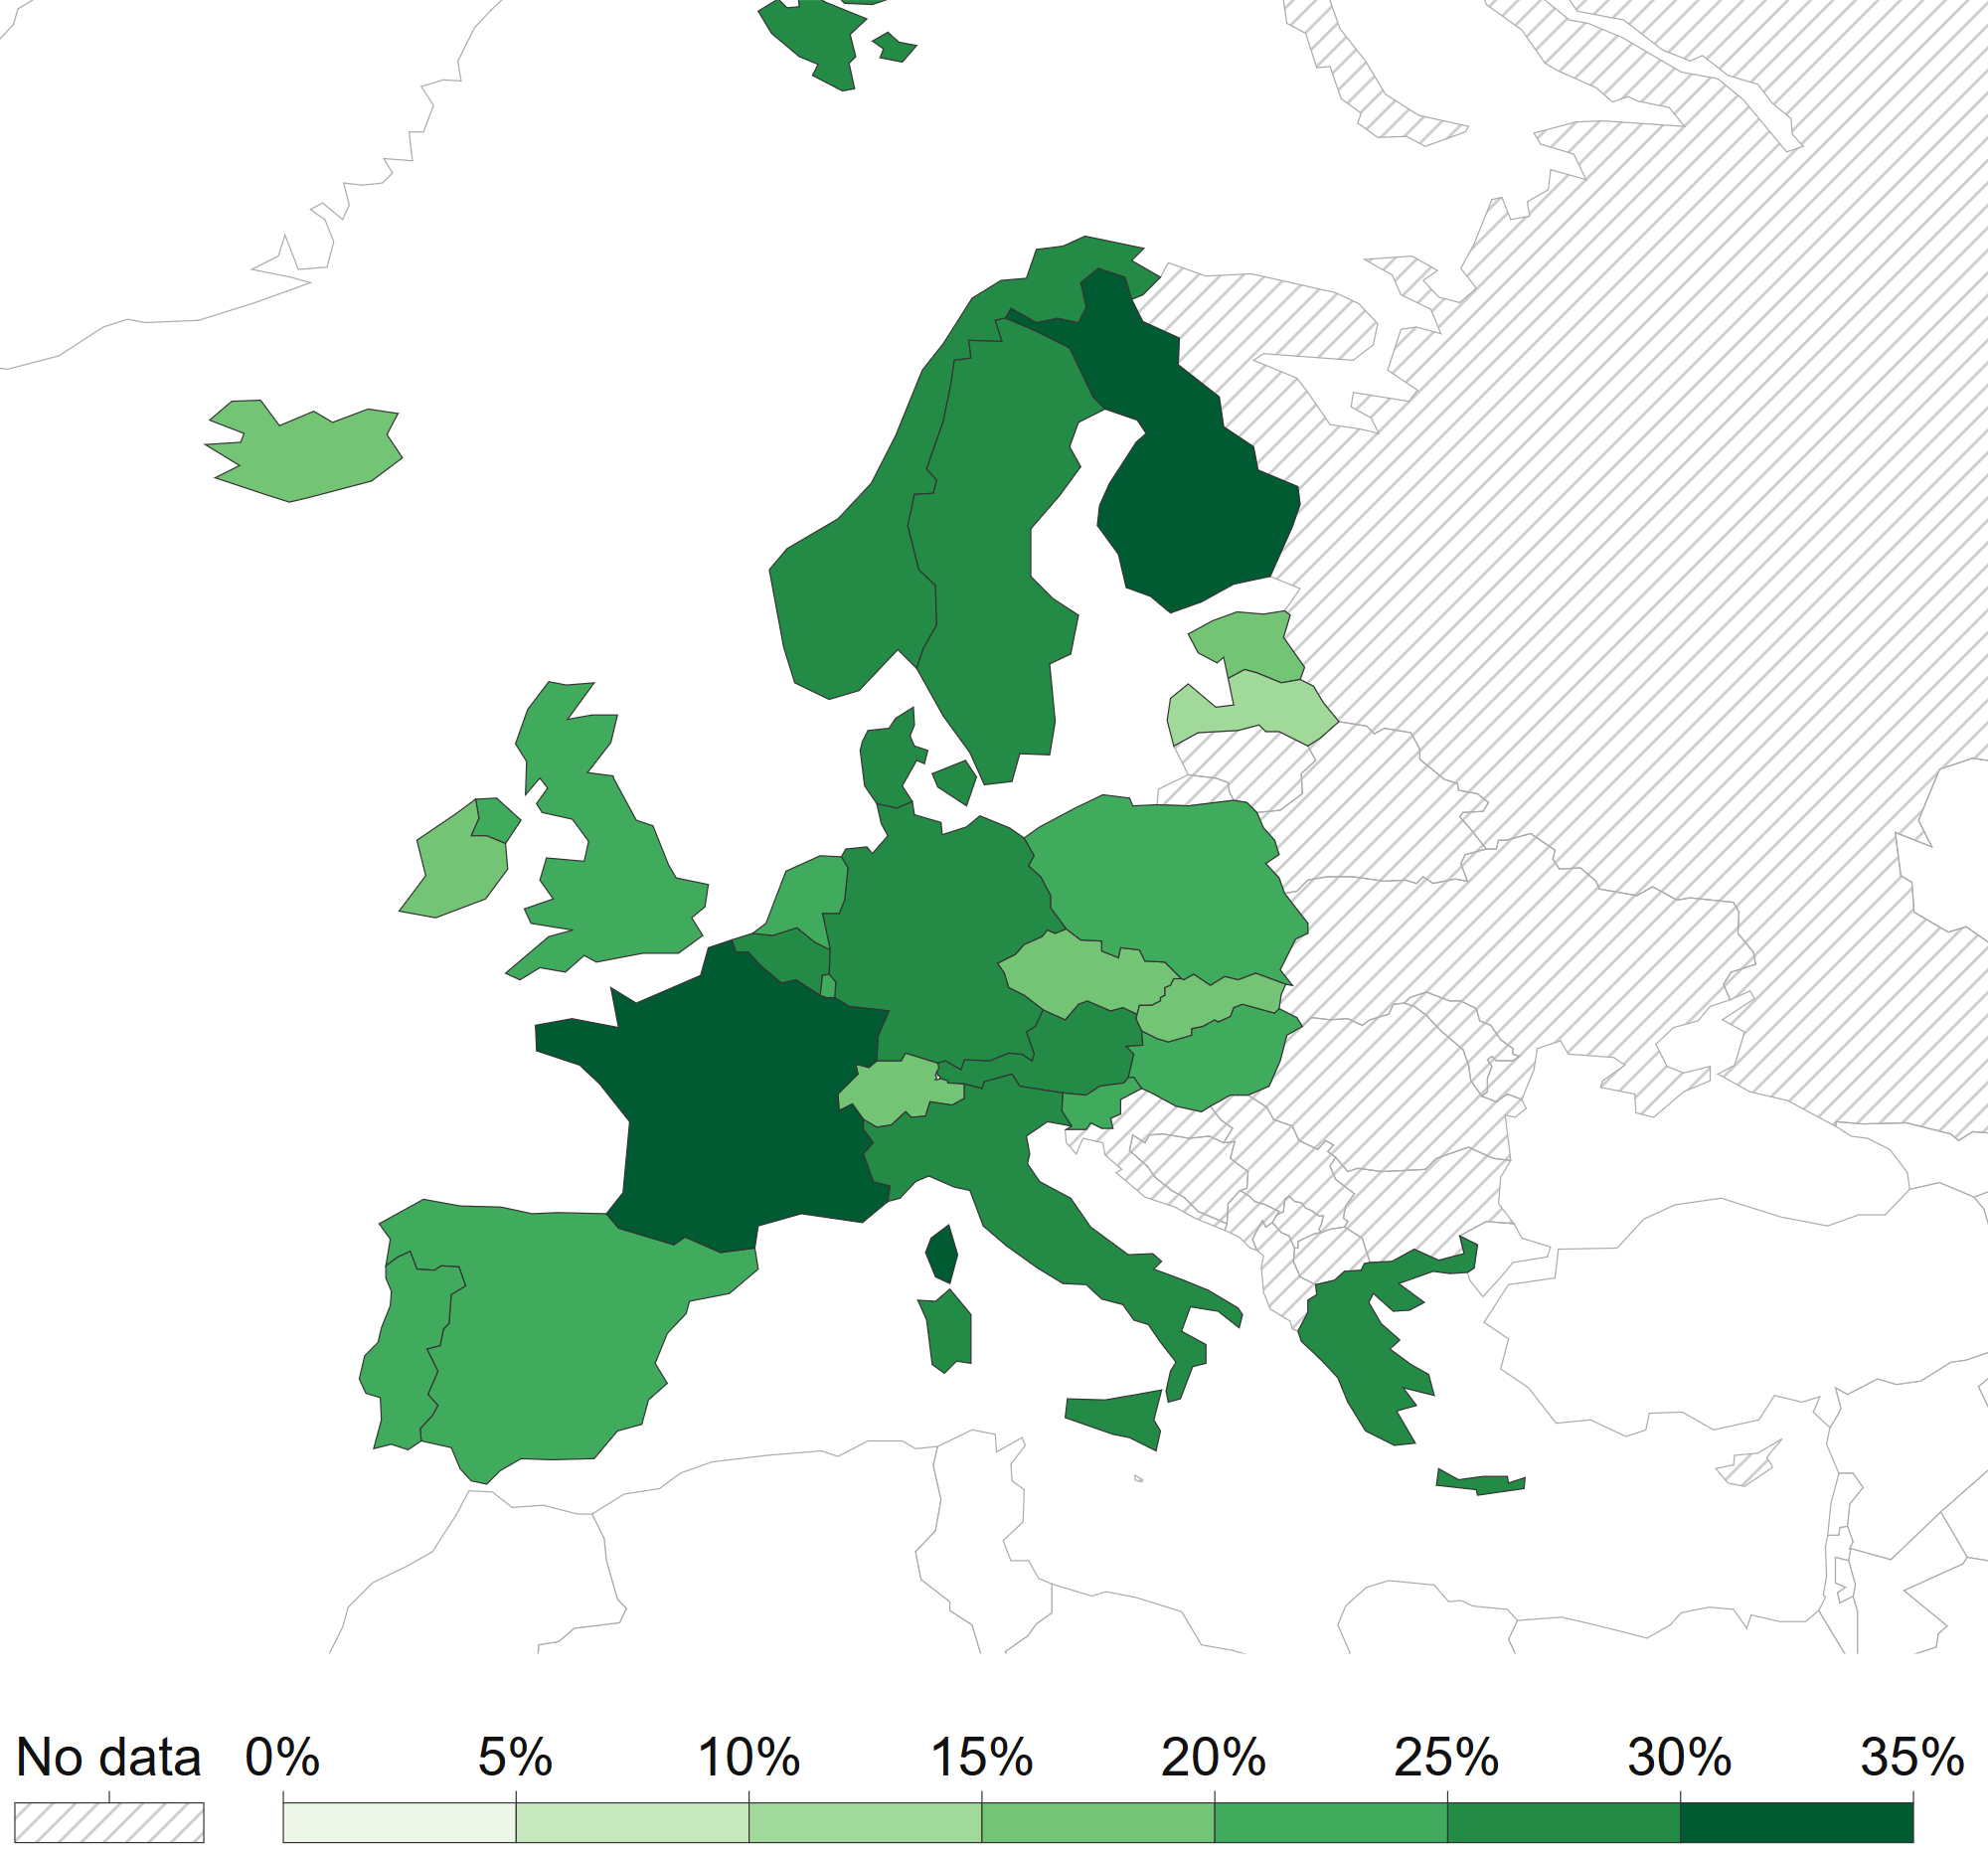
\includegraphics[width=0.8\linewidth]{images/Libro-img029.png}
    \caption{Spesa pubblica sociale in percentuale del PIL, 2016 - Fonte: \protect\url{https://ourworldindata.org/grapher/social-spending-oecd-longrun?tab=map}}
  \end{subfigure}
\end{tabular}
\end{table}

Le strade percorribili sono tantissime. Quotidianamente nascono nuove idee, nuove soluzioni per arrivare pronti al 2050.
Tra le varie proposte c'è quella presentata da Bill Gates il fondatore di Microsoft da anni
impegnato nel sociale con la fondazione Bill \& Melinda Gates. Gates oltre ad essere stato per anni
l'uomo più ricco del mondo (oggi, nel 2020 è il secondo) non si limita semplicemente a fare
donazioni ma a sviluppare soluzioni. Da anni è impegnato in vari progetti tra cui nella lotta alla poliomielite e i
cambiamenti climatici. Gates è un accanito lettore! Riesce a leggere 150 pagine all'ora e questo
gli da una marcia in più nello studio e la comprensione di problemi. Secondo i suoi studi ha intuito che il problema di
fonti rinnovabili come l'eolico e il solare, siccome non possono fornire energia su richiesta, ma
solo quando c'è vento o sole sono difficilmente gestibili. Un impianto sottostimato non fornirebbe
energia sufficiente a tutti mentre se venisse generata corrente in esubero, a lungo andare provocherebbe problemi
all'impianto elettrico. Quando pensiamo alle fonti rinnovabili ci vengono in mente subito queste
due tecnologie, solare e eolico, ma non sono le sole. Le sue letture l'hanno portato a valutare,
l'idea impopolare, di risolvere questo problema con le centrali nucleari. Quando pensiamo alle
centrali nucleari ci viene in mente subito Chernobyl e Fukushima. La nostra mente funziona molto a “immaginari”, così
quando pensiamo al nucleare ci vengono in mente, radiazioni, morte, disastri, bombe ecc… Ma se guardiamo i dati, le
centrali nucleari hanno ucciso molte meno persone rispetto ai tumori provocati dalla combustione di carbone, petrolio e
gas naturali.

\begin{figure}[H]
  \begin{minipage}{17cm}
    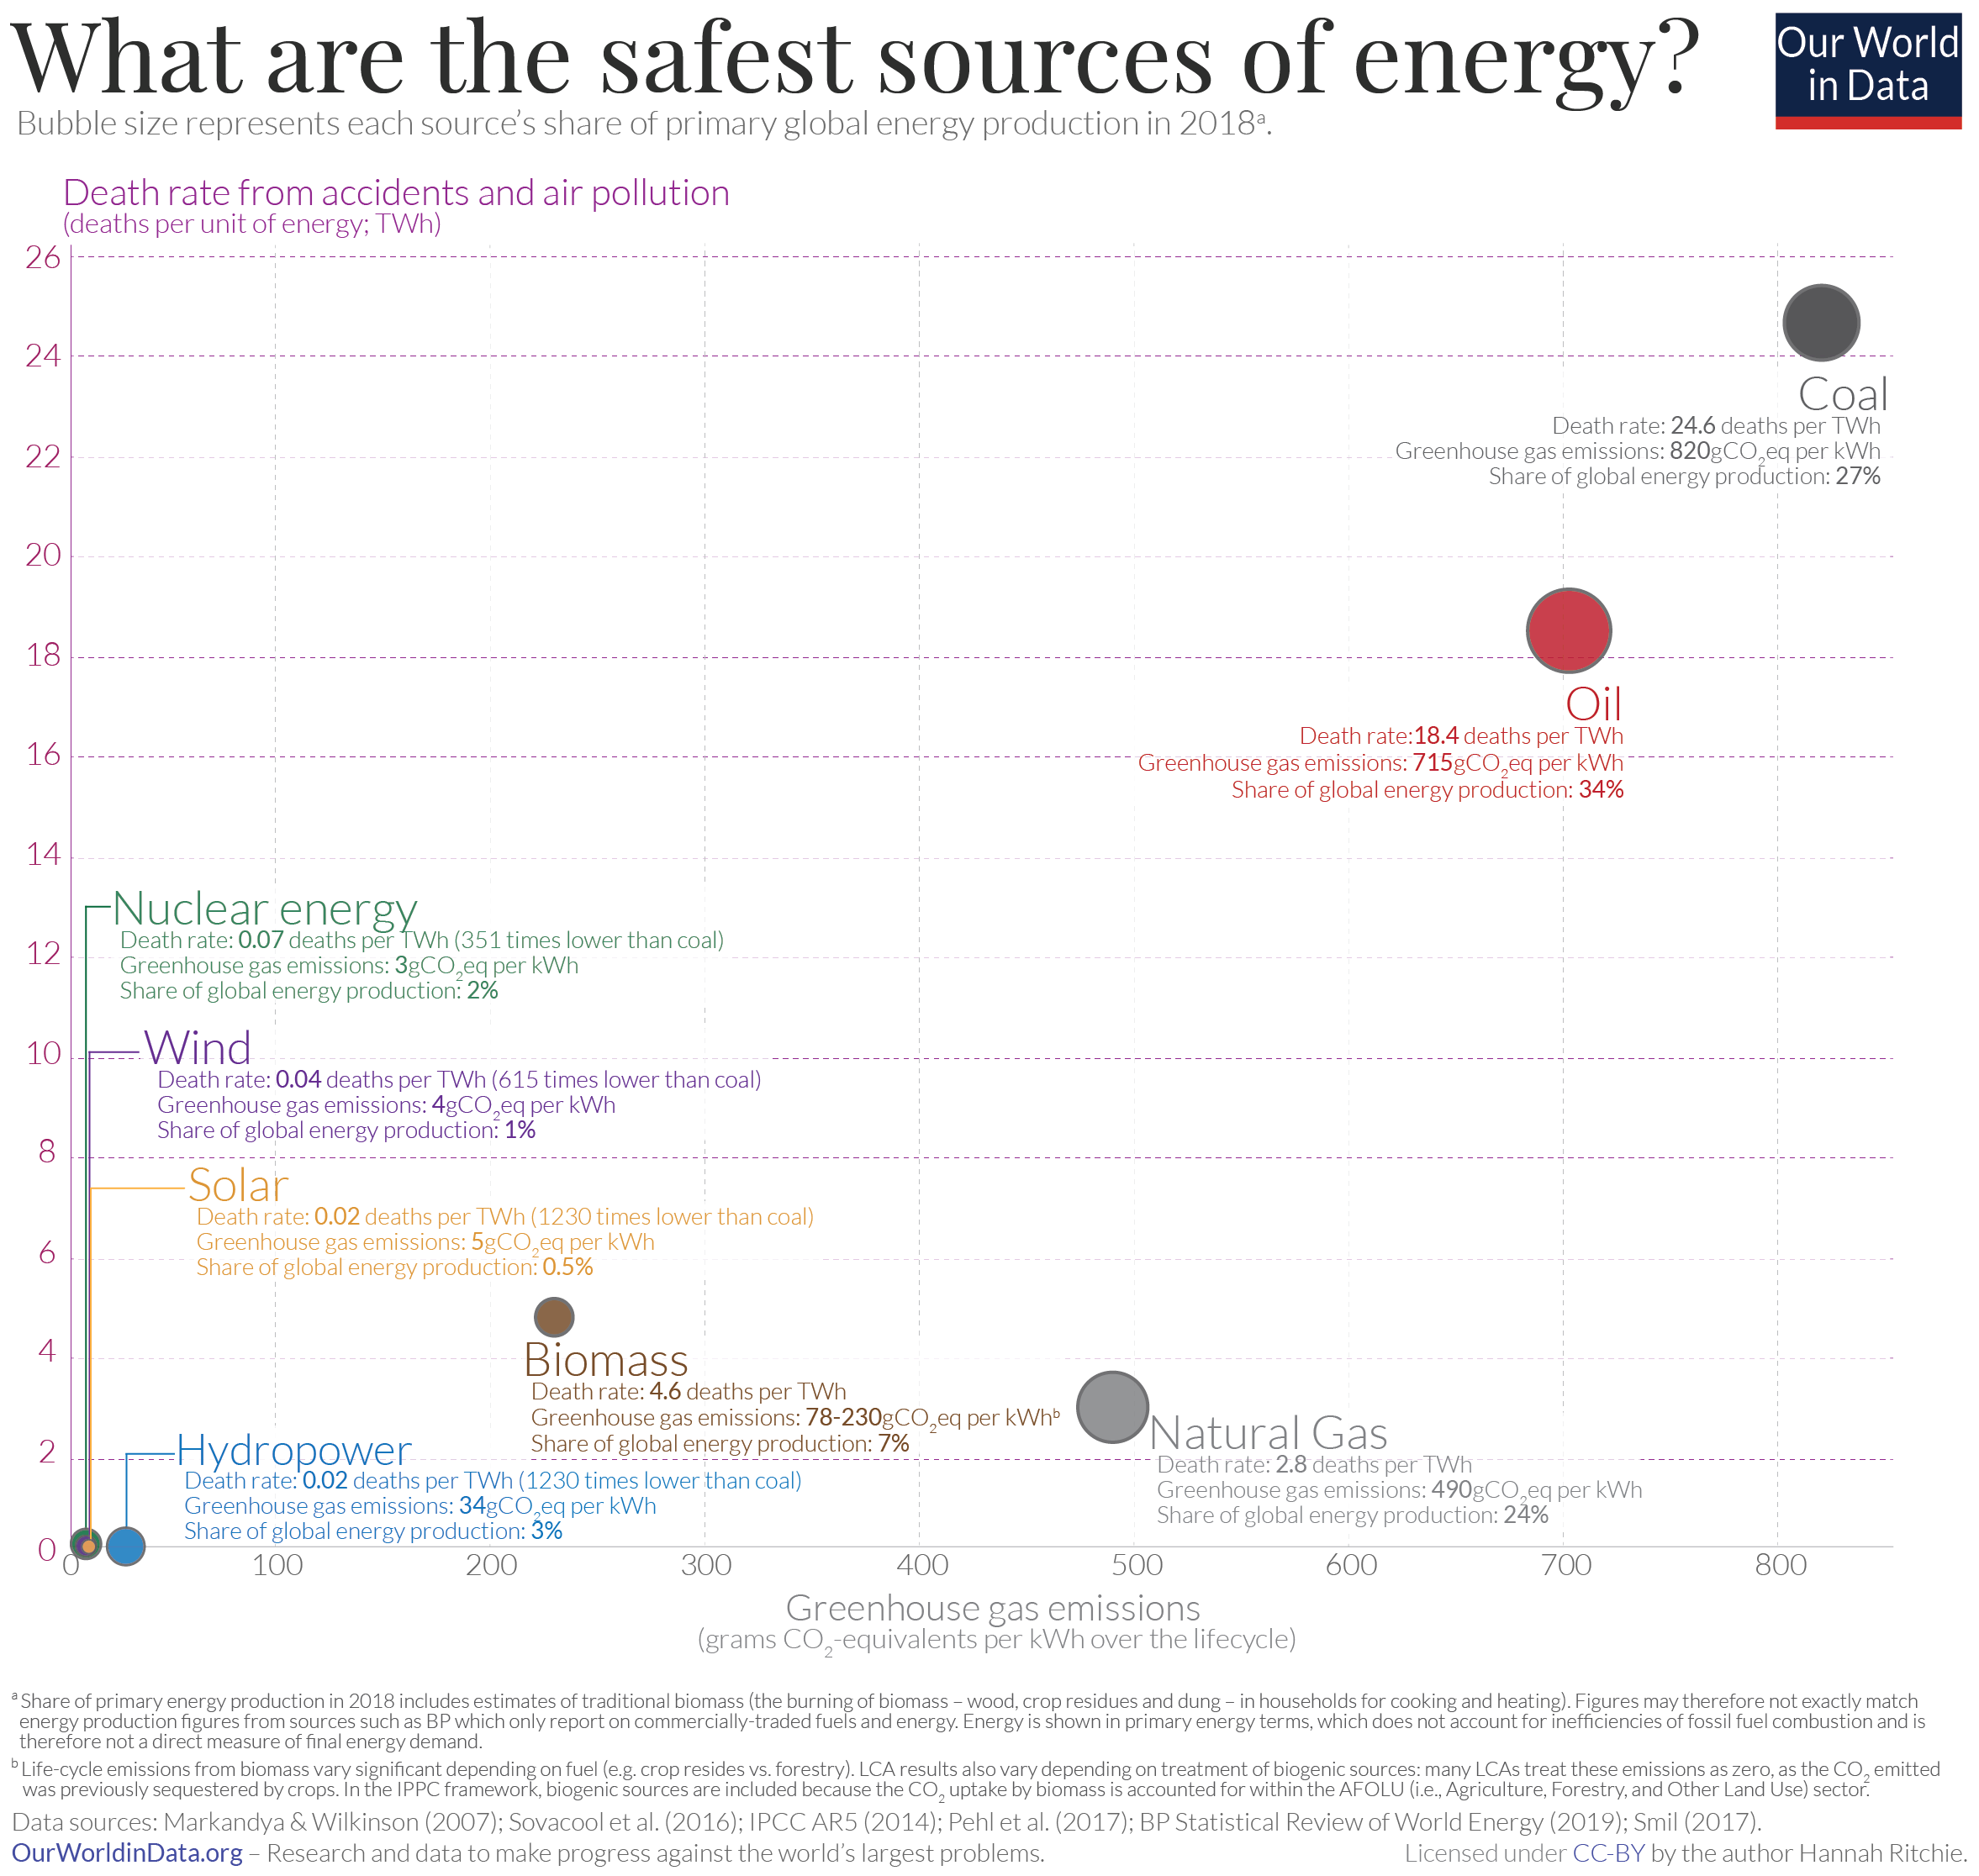
\includegraphics[width=17cm]{images/Libro-img030.png}
    \caption{Credits: \protect\url{https://ourworldindata.org/energy} }
  \end{minipage}
\end{figure}

In questo grafico possiamo vedere sull'asse x i gas serra prodotti dalle varie fonti di energia e,
sull'asse y, il numero di morti che ha provocato ogni terawattora. Vediamo come ci sia una
correlazione tra inquinamento e morte. In testa il carbone, seguito da petrolio, gas naturali e biomasse. Possiamo
notare come il nucleare abbia ucciso molte meno persone rispetto al carbone (351 volte meno). Se consideriamo che
Chernobyl e Fukushima erano centrali nucleari molto vecchie e, che richiedevano molto intervento umano con conseguente
relativo errore, i dati, ad oggi, sarebbero ancora più bassi. Certo, le centrali nucleari producono scorie radioattive,
ma se isolate correttamente non saranno disperse nell'ambiente. Nasce così il progetto
TerraPower\endnote{\protect\url{https://it.wikipedia.org/wiki/TerraPower} } di Bill Gates che si impegna a risolvere questi due
problemi. L'azienda sta sviluppando una nuova tecnologia di reattori, traveling wave reactor o
TWR. Oltre a richiedere il minimo intervento umano, a differenza dei reattori nucleari classici, che utilizzano uranio
arricchito come combustibile, il TWR usa uranio impoverito. Quindi il prodotto radioattivo delle vecchie centrali
nucleari può essere usato per i TWR. Inoltre, come ha spiegato Solomon Goldstein-Rose in un
Ted\endnote{\protect\url{https://www.ted.com/talks/solomon\_goldstein\_rose\_how\_much\_clean\_electricity\_do\_we\_really\_need?language=it}
} non basterà convertire la produzione attuale di corrente da combustibile fossile a fonti rinnovabili, servirà
produrne 12 volte tanto. Questo perché molti strumenti stanno diventando elettrici, nella mobilità e non sono, inoltre
i paesi in via di sviluppo cresceranno, aumentando di conseguenza il loro fabbisogno energetico. In più avremo bisogno
di nuove tecnologie, come quelle impiegate nella rimozione del carbonio prodotto negli anni e, anche questo necessiterà
di energie. Per questi motivi il nucleare sarà indispensabile e forse non sufficiente.

Al contempo, altri ricerche sono contrarie a queste tecnologie in quanto, nel caso dell'Italia, già
ad oggi, come visto nel precedente grafico, produce già il 40\% di elettricità da fonti
rinnovabili\endnote{\protect\url{https://ourworldindata.org/grapher/share-electricity-renewables} }
\endnote{\protect\url{https://www.terna.it/it/sistema-elettrico/statistiche/pubblicazioni-statistiche} }\ e, secondo Enel e The
European House, il nostro paese possa raggiungere la quasi completa decarbonizzazione entro il 2050 e senza bisogno di
energia
nucleare\endnote{\protect\url{https://www.ambrosetti.eu/news/net-zero-e-conomy-2050-roadmap-di-decarbonizzazione-per-leuropa/} \ }.
Chi è contro il nucleare dice che il 2050 è una data troppo imminente contando che si stimano 20 anni per la
costruzione di una sola centrale oltre ad una quantità esorbitante di
denaro\endnote{\protect\url{https://www.vice.com/it/article/bvmdez/centrali-nucleari-in-italia} } e che sottrarrebbe molte risorse
economiche ad altri progetti green. I sostenitori
invece\endnote{\protect\url{https://www.ted.com/talks/isabelle\_boemeke\_nuclear\_power\_is\_our\_best\_hope\_to\_ditch\_fossil\_fuels?language=it}
} portano alcuni esempi, come la Francia che negli anni '70 ha costruito 45 reattori in 15 anni.
Più di recente, Giappone, Cina e Corea hanno costruito reattori in 6 anni circa. Insomma, il tema è complesso, quel che
è certo è che il nucleare fa paura e questo ha portato molte persone a scegliere altri tipi di studi a dispetto
dell'ingegneria nucleare. Bisognerebbe riuscire ad andare oltre queste superstizioni e cercare di
capire in maniera pragmatica quale possa essere una soluzione concreta e sicura. 


\bigskip
\begin{mdframed}[linewidth=1pt]
Attenzione alla lavatrice

Moltissime delle micro plastiche presenti negli oceani arrivano dalle lavatrici. Lavaggi troppo caldi oltre a rovinare
gli indumenti possono separare delle micro fibre dai nostri capi che verranno poi rilasciati
nell'acqua. Una delle migliori scelte ecologiche è proprio impostare un ciclo di lavaggio breve e
con temperature non superiori a 20 °C, utilizzando un additivo igienizzante se vogliamo sentirci più protetti dai
batteri. Oltre all'ambiente questa scelta preserverà più a lungo forma e colore dei vostri capi,
riducendo il rilascio di microfibre sintetiche nell'ambiente fino al 52\% oltre a un consumo inferiore di acqua ed
elettricità. Questo è quello a cui sono arrivati i ricercatori dell'Università di Leeds
(UK)\endnote{\protect\url{https://www.sciencedirect.com/science/article/abs/pii/S0143720819320431} }.
\end{mdframed}

\clearpage\section{Libertà}
Le leggi per la nostra vita sono un “limite”, ma necessarie. Viviamo in uno stato, ma penso in quasi tutto il mondo sia
così, dove non tutte le leggi sono costituzionali, infatti legalità e giustizia non sempre vanno di pari passo.

Le politica economica dovrebbe essere una scienza, come la matematica e, solo esperti nel settore dovrebbero prendere
decisioni in merito, invece capita che persone con qualifiche completamente estranee a questa materia e con non hanno
le competenze per comprenderla (effetto dunning kruger) possano decidere per tutti gli abitanti di uno stato.

Per quanto riguarda le questioni sociali come al solito vediamo che ci sono zone grigie dove non possiamo prendere
decisioni certe ma valutare il miglior rapporto beneficio/rischio e scegliere il compromesso migliore. Consapevoli che
ogni scelta comporta una rinuncia. Tutti questi ragionamenti andrebbero fatti a livello macroscopico in un governo ma
anche nel nostro piccolo come singoli individui partendo da questa regola: 

se non nuoce alla libertà altrui, allora si può fare!


\bigskip

Perché credo che sia importante dare il massimo di libertà a tutti (fino a quando non va a nuocere alla quotidianità
degli altri o all'ambiente)?

Martin Luther King diceva: La mia libertà finisce dove comincia la vostra.

Se tutti diamo il massimo di libertà agli altri; gli altri dovranno dare il massimo di libertà a noi. Questo può
richiedere uno sforzo, io per esempio sono un maschio, bianco, occidentale, battezzato, eterosessuale ecc… Io non
faccio parte di nessuna minoranza quindi non avrei nessun vantaggio nel ritenere giusta la parità di genere, razza,
religione, orientamento sessuale o essere pro droghe, aborto ecc… 

Tutte queste caratteristiche non sono un merito, ci sono nato così, sono sempre stato un nemico delle iniquità di ogni
genere, per cui mi viene naturale essere a favore della parità fra i sessi, religioni, razze, orientamento sessuale,
anche se oggettivamente non ho nessun vantaggio pratico, se non quello del poter vivere in una società che orientata
con questo pensiero farà anche altre scelte che saranno poi positive per me. Posso capire però che venga naturale per
tutti, per questo è richiesto uno sforzo. Io, come altri, non ho nessun merito se sono un maschio, bianco, occidentale,
battezzato, eterosessuale, non sono cose che ho guadagnato con lo studio, il lavoro, la pratica o
l'impegno, ci sono nato così, per uno strano e fortuito (socialmente parlando) scherzo del
destino. Sarei potuto nascere femmina, nera, mussulmana e lesbica, esisteranno tante persone così e, come essere umani
valgono come me, pari uguali a me, e hanno bisogno di essere felici come me. Nel mio piccolo, parlando con le persone è
importante per me farmi promotore della giustizia, dell'uguaglianza e della libertà di tutti anche
se non cambierò le cose. 

Siamo portati a pensare che essere gentili, protettivi e dare un occhio di riguardo a donne, omosessuali, immigrati ecc…
sia un comportamento nobile. E lo è, ma può avere degli effetti collaterali. In primo luogo si calcifica e si consolida
l'idea che le donne o i neri necessitino dell'aiuto e della compassione e che
altrimenti da soli, senza la mano generosa dell'uomo o dell'occidentale, non
possano farcela. Il secondo problema è che, anche se in modo innocente, ingenuo e generoso, rimarca che comunque una
differenza c'è. Tra uomini e donne, tra bianchi e neri ecc… Anche frasi dette per ridere come: chi
dice donna dice danno, noi donne siamo multitasking, donna al volante pericolo costante, gli uomini pensano solo a
quello ecc… Se si parla di una differenza, la si rimarca, vogliamo che ci sia e nessuno vuole essere al secondo posto.
Mi spiace vedere ragazze che hanno smesso di lottare per la loro emancipazione. Dove il loro femminismo si ferma solo
nel dire che dietro un grande uomo c'è una grande donna e, poi si comportano esattamente come
farebbe un misogino, dandosi delle zoccole, screditandosi a vicenda e, cercando la dipendenza di un uomo.


\bigskip
\begin{mdframed}[linewidth=1pt]
Femminismo

Il femminismo viene percepito come il contrario del maschilismo, quindi come un movimento che mira a puntare la
supremazia del genere femminile a discapito di quello maschile, in termini di diritti e opportunità. Originariamente e
tutt'ora il femminismo invece si batte per la parità, non solo dei sessi ma di qualsiasi
minoranza. Quindi tutti dovremmo essere femministi, ma ultimamente questo movimento sembra dimenticare sempre di più il
suo scopo originario. 

Sul web o comunque più in generale nel dibattito pubblico troviamo due schieramenti, quelli che dicono che le donne sono
più svantaggiate sempre e comunque in ogni ambito e quelli che invece dicono che sono i maschi. Quello che vorrei fare
di seguito è portare evidenze che rimbalzando da un polo all'altro mostrino che possiamo trovare
svantaggi e vantaggi in donne e uomini anche negli stessi ambiti, per dire che il discorso è più complicato di così. 

Partiamo dai casi meno noti, quelli in cui l'uomo è sfavorito rispetto alla donna e come vedremo lo
è su cose importanti, addirittura come la mortalità sul luogo di lavoro. Secondo i dati
Inail\endnote{\protect\url{https://www.inail.it/cs/internet/docs/alg-dati-inail-2021-giugno-luglio-pdf.pdf} } nel 2021 sul posto di
lavoro sono morti 1.366 uomini contro 72 casi per le donne. Questo è per colpa del femminismo che è andato troppo oltre
ottenendo troppi poteri? No! semplicemente gli uomini sono biologicamente favoriti nei lavori più duri che sono anche
quelli più rischiosi. Anche per quanto riguarda i senzatetto il fenomeno è principalmente maschile 84\% contro il 16\%
delle donne\endnote{\protect\url{https://it.wikipedia.org/wiki/Senzatetto} } a volte correlato da un altra disparità, ovvero quella
giuridica, che nelle separazioni porta gli uomini a perdere la casa e parte del reddito. Infatti non esistono leggi che
favoriscono il maschio, ma ne troviamo diverse che favoriscono la donna, come nei divorzi, ottenere lo sconto di pena
ai domiciliari, quote rosa ecc… Quindi questa è una disparità tra i sessi anche nella legge? No! Al contrario, esistono
differenze biologiche tra maschio e femmina e per mitigare queste differenze bisogna intervenire sulla legge, come ad
esempio il divieto di licenziamento per matrimonio e gravidanza, in quanto un maschio, per ovvie ragioni, non sarà mai
licenziato per la gravidanza, mentre una donna, senza questa legge, potrebbe rischialo. I tassi di suicidio sono
maggiori per gli uomini rispetto alle donne ma al contempo sappiamo che la depressione sia un fenomeno più femminile.
Quindi gli uomini sono più fragili? O forse hanno pressioni sociali circa il macismo, da parte di uomini e donne? O
forse le donne culturalmente e legalmente vengono aiutate di più da mariti, familiari e amici? Non lo so, lo scopo di
queste righe è proprio mostrare quanto la questione sia più complicata di come il dibattito pubblico spesso vuole
dimostrare. 

Tra le varie obiezioni che si fanno al femminismo troviamo che nella comunicazione si parla solo di quando una donna
muore sul posto di lavoro, nonostante abbiamo visto siano una forte minoranza rispetto a quelle femminili. Questa
informazione solitamente viene posta come a dire: basta tutelare le donne, le abbiamo tutelate anche troppo! Invece
quello che vorrei comunicare è che esistono differenze gravi, sia da una parte che dall'altra, è
inutile negarlo, anzi, portiamo tutti i problemi all'attenzione in modo da trovare una soluzione.
Parlare dei problemi maschili non nega quelli femminili e viceversa.


\bigskip

Anche socialmente esistono differenze a volte contraddittorie. Quando si parla di mercificazione del corpo femminile si
ritrova nei maschi la principale causa di questo problema, quando invece certi inestetismi vengono notati più dalle
donne che dagli uomini. Anche il corpo maschile sempre di più sta raggiungendo degli standard impossibili, anche la
fortuna genetica non è più sufficiente, l'allenamento non è più sufficiente senza anabolizzanti. O
ancora, quando si può utilizzare il proprio fascino per evitare una multa dopo essere stati fermati dalla polizia,
alimentando l'oggettificazione del corpo.

Per alcune la donna deve essere una principessa e l'uomo deve farla sentire tale, mentre il contrario non è usuale.
Dire: “non sto con un uomo basso, perché altrimenti non posso mettere i tacchi” è facile da dire, non ci si aspetta che
qualcuno possa rimanerne ferito o vergognarsi (ma per quale valore?). Ma non è esattamente come dire: “io non voglio
stare con una ragazza grassa”? Invece questo scatenerebbe le ire dei più, che potrebbero additarti come superficiale
nel migliore dei casi. 


\bigskip

Parlando di occupazione e salari le cose diventano ancora meno dicotomiche. Da una parte troviamo chi dice che in Italia
la differenza di salario tra uomini e donne è tra le più basse in
Europa\endnote{\protect\url{https://ourworldindata.org/economic-inequality-by-gender} }, dall'altra parte però
sappiamo che la disoccupazione femminile in Italia è tra le più alte in
Europa\endnote{\protect\url{https://en.wikipedia.org/wiki/Women\_in\_the\_workforce\#/media/File:Unemployment\_rate,\_women,\_OWID.svg}
}, inficiando così anche sul calcolo per la differenza di salario. Allora si introducono le quote rosa, però così
andiamo sottrarre valore al merito. Però non è normale che se le donne si iscrivono di più in università e completano
il percorso di laurea più degli uomini poi trovino meno lavoro. Però le donne si laureano più su materie umanistiche
dove c'è meno richiesta e stipendi più bassi rispetto alle materie tecniche. Però alcuni studi
dimostrano che la società porta di più le donne a preferire materie umanistiche e vengono scoraggiate ad affrontare
materie matematiche. Insomma, essere certi di aver trovato la ragione, dimostra una certa leggerezza, superficialità e
un modo sbrigativo di trovare una risposta. 


\bigskip

Lo studio che accennavo prima si è chiamato “draw scientists”, che prevedeva di far disegnare a dei bambini uno
scienziato. Nel 1980 tutti i bambini e le bambine disegnarono uno scienziato maschio, solo lo 0.6\% rappresentò una
femmina. Uno studio di David I. Miller del
2018\endnote{\protect\url{https://srcd.onlinelibrary.wiley.com/doi/full/10.1111/cdev.13039} } ha replicato
l'esperimento portando la percentuale al 28\%. Sicuramente c'è stato un forte
miglioramento, ma siamo ancora lontani dalla parità. Lo studio è più semplice da somministrare in inglese rispetto
all'italiano in quanto chiedere di disegnare uno scienziato potrebbe portare i bambini a disegnare
un maschio. Sarebbe più corretto chiedere: disegnate uno scienziato o una scienziata. In inglese questo problema non si
pone. Quindi se poche donne lavorano in campi scientifici, non dipende dai datori di lavori maschilisti, ma da
stereotipi che già da piccoli interiorizziamo e crescendo con essi ci faranno fare scelte diverse.

Allo stesso tempo però ci sono difficoltà da entrambi i lati in quanto le famiglie donano più scelta circa la propria
formazione alle donne rispetto agli uomini. Questo dipende dalle aspettative sociali che si hanno sugli uomini.
L'uomo infatti è quello che “deve” portare i soldi a casa e (anche per alcune donne) guadagnare
più della donna. O ancora, un uomo che sta a casa dei genitori dopo i 30 anni è un mammone, mentre il giudizio non è
altrettanto aspro per le donne. Così tutte le scelte formative e professionali sono volte a questo scopo, più che alla
propria crescita
personale\endnote{\protect\url{https://www.barinedita.it/bari-report-notizie/n4469-i-corsi-universitari-ce-ne-sono-di-} }.


\bigskip

Questo porta in parte anche alla differenza di salario tra uomini e donne. I lavori scientifici infatti sono più pagati
rispetto alle materie umanistiche. Questa è una delle critiche che vengono poste quando si parla di differenza di
salario. Secondo alcuni infatti questi calcoli vengono fatti semplicemente sommando gli stipendi di uomini e donne e
vedendo la differenza in percentuale, senza contare la tipologia di lavoro, le ore di lavoro, siccome il part time è
più diffuso tra le donne ecc… spesso in tanti indici è così, in alcuni indi più seri invece non
c'è differenza\endnote{An economist explains why women are paid less
\protect\url{https://www.weforum.org/agenda/2019/03/an-economist-explains-why-women-get-paid-less/} }, altri studi invece spiegano
che qualsiasi formula si scelga per misurare il divario retributivo emerge sempre una
disparità\endnote{\protect\url{https://www.epi.org/publication/what-is-the-gender-pay-gap-and-is-it-real/} \ }. Oltre a questi
fattori misurabili, concorrono a differenziare gli stipendi anche dinamiche culturali meno calcolabili. Se un uomo, ad
esempio, contratta lo stipendio, risulta ambizioso, se lo fa una donna la percezione non è altrettanto positiva per
qualcuno.


\bigskip

Anche rimanendo su dei clichè gli uomini possono fare lavori più duri e andare in guerra mentre le donne sono più
orientate all'ascolto, all'empatia, ma ciò non toglie che ci siano tanti
uomini sensibili e donne determinate. Entrambi i sessi, con le loro caratteristiche più adatte per determinate
situazioni, se in collaborazione possono portare avanti il progetto comune dell'essere umano.
Rimanere su una narrativa che gli uomini sono meglio per questi motivi o che le donne sono migliori per queste altre
argomentazioni, frena ciò che possiamo fare come esseri umani, mentre, più che evidenziare e rivendicare le nostre
differenze, dovremmo metterle a servizio degli altri in un ottica collaborativa tra i sessi non nonostante le nostre
differenze, ma proprio in virtù di queste ultime. 

Quello che non deve succedere e che ogni tanto mi sembra che stia succedendo è che diventi una gara maschi contro
femmine. L'ideale sarebbe studiare le differenze biologiche, culturali, caratteriali tra uomini e
donne e collaborare gli uni con gli altri in modo che i pregi di uno siano arricchenti per
l'altro. Tanti uomini sono sensibili per la questione femminile e viceversa. Troviamo donne in
disaccordo con le quote rosa, che nell'atto di emancipazione rigettano questi aiuti, come se da
sole non potessero farcela.
\end{mdframed}

\bigskip

Il mondo che abbiamo creato è il prodotto del nostro pensiero e dunque non può cambiare se prima non modifichiamo il
nostro modo di pensare (Albert Einstein).


\bigskip

Parlando dei dibattiti abbiamo visto quanto sia difficile per chiunque cambiare idea e quanto possa influire il fattore
culturale in una decisione riguardante per esempio i matrimoni gay. Per alcune persone però sembra essere
biologicamente difficile uscire dagli schemi. Una ricerca della University of Queensland e della University of
Pennsylvania\endnote{\par
\protect\url{https://qz.com/574353/do-you-see-a-square-research-says-this-simple-test-can-predict-your-political-beliefs/} } spiega
che le persone che hanno una concezione rigida della sfera morale o sociale, come ad esempio inquadrare il matrimonio
solo all'interno di una coppia di sessi opposti, cosi farebbero con tutte idee, fino ad arrivare alla geometria.
Osservando figure geometriche distorte, i conservatori avrebbero infatti maggiori difficoltà a classificarle come
cerchi, quadrati o triangoli.

Questa figura infatti potrebbe dire se sei a favore o contro i matrimoni gay:


\bigskip



\begin{figure}[H]
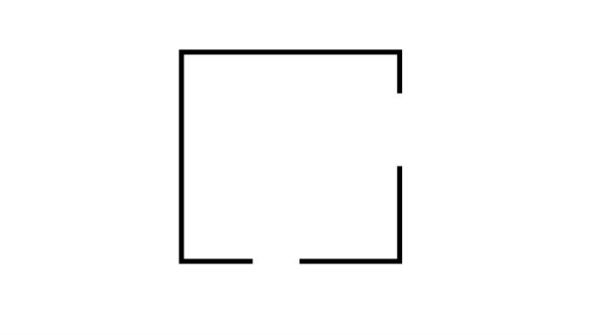
\includegraphics[width=15.875cm,height=8.864cm]{images/Libro-img031.png}\end{figure}

\bigskip

Agli occhi di un conservatore è intollerabile qualunque tipo di irregolarità, poco importa se si tratta di matrimoni
gay, di un immigrato, o di una forma geometrica irregolare.


\bigskip

Un esempio di come le esigenze personali a volte siano contrarie a quelle sociali? Il North Carolina e il Mississippi
oltre a essere ai primi posti per omofobia e non dare diritti agli omosessuali sono anche al primo posto per fruizione
e acquisto di porno gay e trans. Secondo il sito per adulti GameLink, il porno più venduto in North Carolina è My TS
[Transsexual] Teacher, seguito da Shemale Shenanigans, a sua volta seguito da Joey Silvera's Trans-Visions 6.
{\textquotedbl}Dal 2012 la crescita del pubblico di porno trans in North Carolina è stata esponenziale,{\textquotedbl}
ha detto Jeff Dillon, vicepresidente della compagnia madre della GameLink, la eLine. Mentre in Mississippi i cinque
porno più visti sono Full Service Transsexuals, Fathers and Sons Number 3, Bareback Sex, Daddy and Me, e il sempreverde
Joey Silvera's Trans-Visions
6\endnote{\protect\url{https://www.vice.com/it/article/wdwm75/gli-stati-omofobi-sono-anche-quelli-che-scaricano-piu-porno-trans-e-gay}
}.


\bigskip

Un altro studio condotto da John R. Alford, Carolyn L. Funk, John R.Hibbing nel 2005 pubblicato su Apsa e edito da
Cambridge University
Press\endnote{\protect\url{https://digitalcommons.unl.edu/cgi/viewcontent.cgi?referer=https://www.google.com/\&httpsredir=1\&article=1006\&context=poliscifacpub}
} ha analizzato le opinioni politiche di 12.000 gemelli negli Stati Uniti e in Australia. I dati hanno messo in luce
che i gemelli identici hanno maggiori probabilità di concordare su questioni politiche rispetto ai gemelli fraterni.
Ovviamente la genetica non è tutto, infatti indicativamente ogni cinque anni vince la fazione opposta a quella attuale
nel sistema bipartitico. Però c'è sicuramente una predisposizione che non è solo quella
culturale\endnote{\protect\url{https://www.stateofmind.it/2019/06/orientamento-politico-genetica/} }.


\bigskip

Come al solito per me vale la regola del: Se non nuoce alla liberà e alla quotidianità della società allora è
consentito. Ma come abbiamo visto parlando di libero arbitrio raramente siamo noi a decidere in maniera consapevole,
spesso dipende dai nostri bias cognitivi, dalle nostre emozioni e dai nostri schemi mentali.


\bigskip

Quindi sono pro ai matrimoni gay, ma per le adozioni? Qua non mi sento di esprimere una mia idea ma affidarmi a quanto
scritto nel
dossier\endnote{\protect\url{http://www.voxdiritti.it/stepchild-adoption-dagli-psicologi-un-dossier-che-dimostra-come-lomogenitorialita-non-influisca-sul-benessere-psicologico-dei-figli/}
} presentato dall'Ordine degli Psicologi del Lazio contenete oltre 70 studi, svolti tra 1972 e il 2015. 

Il presidente dell'Ordine degli Psicologi del Piemonte, Alessandro Lombardo, Spiega che per la salute psicologica del
bambino non ci sono problemi a crescere all'interno di una famiglia arcobaleno: {\textquotedbl}Il
vero problema nel crescere in famiglie omogenitoriali, ciò che le differenzia dalle altre famiglie, è il contesto più o
meno omofobico nel quale vivono. Questo, sì, fa la differenza. Per il resto, saranno buoni genitori, pessimi genitori,
come lo possiamo essere tutti. [...] Non esiste, se non nei codici culturali, un unico modello di famiglia. È chiaro
quindi che il salto è culturale, del tipo di società che vogliamo e dobbiamo
essere.{\textquotedbl}\endnote{\protect\url{https://www.vice.com/it/article/5gn7ba/intervista-ordine-psicologi-vendola-778} }


\bigskip

Pensando ad una società più equa un filosofo di Harvard ha immaginato di ordinare una pizza: come fate a sapere che non
vi toccherà la fetta più piccola? Bisogna fare in modo che chi taglia la sarà l'ultimo o tra gli ultimi a mangiare, in
questo modo si sforzerà di fare fette di dimensioni simili. Allo stesso modo bisogna pensare a una società senza sapere
dove ci collocheremo in termini di sesso religione età etnia orientamento sessuale ecc… 


\bigskip
\begin{mdframed}[linewidth=1pt]
Quando satira, ironia e black humor vanno oltre?

Molto spesso è difficile fare qualcosa di divertente senza ledere qualcuno. Anche uno scherzo ad un amico deve, almeno
in maniera minima lederlo, perché si spaventa, perché viene bagnato, perché gli nascondiamo qualcosa ecc… La satira e
il black humor sono gli esempi principali di comicità che si basano sul ledere qualcosa. Queste modalità comiche sono
le più rischiose perché vanno a toccare argomenti su cui l'opinione pubblica è più sensibile, come
guerra, disabilità, morte, malattia, orientamento religioso, sessuale, discriminazioni razziali, di genere, violenze
sessuali anche su minori. Non è un caso che le tematiche siano così sensibili, perché uno degli scopi della satira è
proprio quello di portare le persone a ragionare su certi temi, usando la comicità come pretesto per arrivare ad un
pubblico più vasto. Un altro degli obiettivi che si prefigge la satira è quello di stemperare e cercare di portare un
sorriso anche nel dramma. La satira e il black humor cercano di sovvertire il perbenismo, il politicamente corretto, il
bigottismo e tutto ciò che culturalmente è sempre stato un tabù. Tutto ciò che è soggettivo o che culturalmente non si
può toccare la satira lo va toccarla apposta. Quasi come un esercizio atto a liberarsi da questa morale che ci dice in
cosa credere, cosa è giusto e cos'è sbagliato, in maniera cieca senza possibilità di rimetterla in
discussione. 

Ma quando questa comicità si spinge oltre? Il fatto che qualcuno si senta offeso non può essere un metro di giudizio,
specialmente in questo periodo, lo possiamo vedere sulla rete, la gente si offende per tutto, sia che si critichi una
squadra di calcio fino al beniamino della serie TV. Quindi per qualcuno satira e black humor sono una modalità di
espressione che non ha limiti.

Dall'altro lato si usa il black humor in maniera un po' furba in alcuni casi e
un po' pavida negli altri. Su internet circolano meme di Black humor dove però al loro interno non
sono presenti elementi comici, rimanendo così solo il black. Questo tipo di tentato umorismo cerca di degradare e
deridere la sofferenza altrui. In questi casi la domanda che sorge spontanea è: perché senti il bisogno di svilire
qualcuno gratuitamente? Se non c'è umorismo, non c'è una critica sociale, cosa resta? Mancano proprio gli elementi
umoristici che possono essere dei giochi parole, situazioni paradossali, doppi sensi, ironia ecc… Sono solo un insieme
di termini culturalmente mal visti che orbitano attorno alla discriminazione sessuale, di genere, razziale, religiosa
con l'aggiunta di qualche malattia difficilmente curabile. Ma senza almeno un elemento comico cosa
resta? Sono solo parole culturalmente borderline, come i bambini che ridono sentendo “cacca, mutande, scoreggia” (lo so
che hai appena riso). Il meccanismo a questo punto prevede che se non ridi è colpa tua perchè sei un boomer, un
bigotto, una persona triste, uno senza umorismo ecc… non perché la battuta non fa ridere.

Altre volte si vuole insultare una persona o un gruppo e, quando gli altri si arrabbiano ci si mette in salvo con la
scusa: era solo una battuta!


\bigskip

Bisogna chiedersi: cos'è che c'è di divertente? Qual è l'elemento comico oltre al lessico e al
toccare tematiche sensibili? Se non si riesce a trovare un motivo, allora forse sono stati gli altri a dirci che è
divertente. E così ridiamo della morte, delle guerre e delle malattie riducendoli a meme, credendo di emanciparci ma
finendo per conformarsi. Quando la satira non ha un messaggio di denuncia, spesso la usiamo per tentare di esorcizzare
qualcosa che ci spaventa ma con l'effetto di svilire qualcosa di importante che ci riguarda. A volte ridiamo di un meme
tragico, per non affrontare quanto quella cosa abbia a che fare con noi. Detto questo non voglio demonizzare il meme o
il black humor, ma se reagiamo come reagirebbero tutti non siamo più autentici.
\newline
\newline
Quindi secondo me la domanda chiave è: quali sono le intenzioni che portano una persona a fare una certa battuta? Non
dobbiamo soltanto con lo scopo di interpretare il comportamento degli altri, ma anche il nostro. Lo scopo era quello di
strappare una risata anche alla persona/gruppo a cui era diretta la battuta? O quello di stimolare una riflessione? O
solo di ferire qualcuno? Questa consapevolezza fa tutta la differenza a mio avviso. Inoltre accorgiamoci anche quando,
parlando con le altre persone, se il tono è serio, se sentiamo l'esigenza di portare la
conversazione sul lato divertente e quanto spesso. Questo è un indicatore di quanto sappiamo affrontare anche le cose
serie o le vogliamo solo evitare.


\bigskip

Una battuta fatta ad un gruppo di amici o ad un pubblico più vasto che può essere uno spettacolo dal vivo, la TV, la
carta stampata o i social network deve avere un attenzione diversa. Se facciamo una battuta coi nostri amici, dove noi
conosciamo la loro sensibilità, su cosa si può scherzare e su cosa no e dove loro conoscono il nostro pensiero a
riguardo, ad esempio se facciamo una battuta razzista e i nostri amici sanno che non lo siamo, ha un peso diverso
rispetto ad una battuta fatta da un razzista. Poi uno potrebbe sempre dire, non è affar mio se questa persona si
offende perché legata a delle vecchie idee culturali di cosa si può dire e cosa no. Ma la domanda è sempre quella: qual
è il tuo obiettivo? Farlo ridere? O rovinare il vostro rapporto? Ne vale la pena?


\bigskip

Quando invece il nostro pubblico diventa più grande dobbiamo avere molte più attenzioni, ma solitamente abbiamo il tempo
di prepararle prima di farle. Dietro ad una battuta spesso ci sono ore di studio per trovare il giusto equilibrio tra
ironia e spunti di riflessione. Con questo non possiamo limitare l'umorismo ai soli
professionisti, ma sarebbe intellettualmente onesto che qualsiasi battuta ironica fosse frutto di
un'elaborazione volta a evitare fraintendimenti. Più il pubblico è grande più le probabilità che
qualcuno si offenda sono maggiori, nonostante tutte le attenzioni che si possono aver messo nella creazione della
battuta. Anche qua è giusto chiedersi: ne vale la pena? Il messaggio che voglio dare è abbastanza importante da
giustificare l'ira di qualcuno? Questa battuta porterà più persone a ridere o a riflettere
rispetto a quello che invece farò arrabbiare?

\begin{wrapfigure}{i}{9cm}
  \centering
  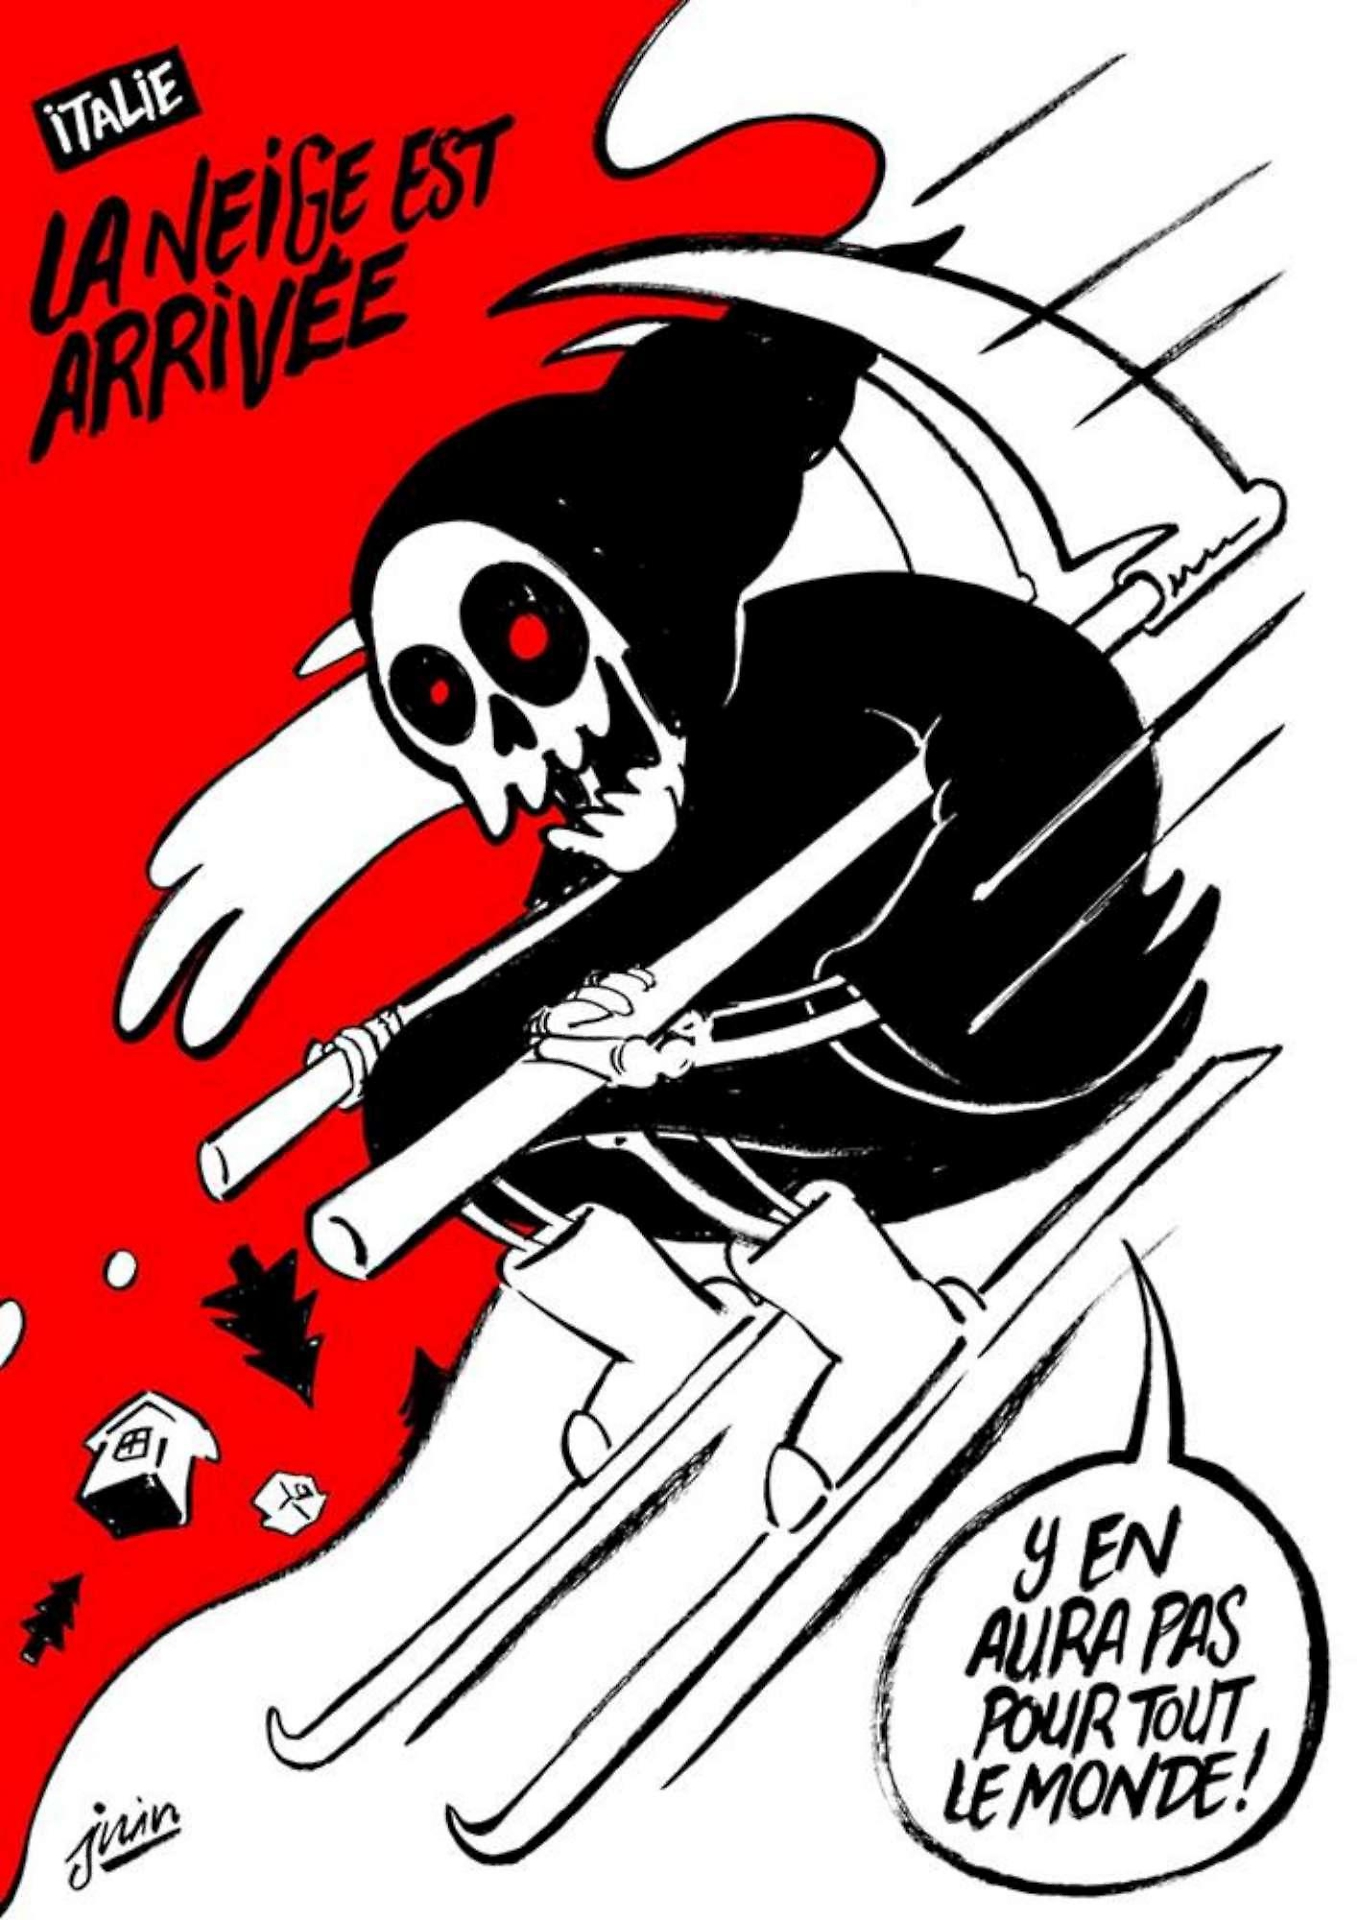
\includegraphics[width=0.95\linewidth]{images/Libro-img032.jpg}
  \begin{minipage}{\linewidth}
    \caption{Vignetta satirica tratta dal giornale Charlie Hebdo}
  \end{minipage}
\end{wrapfigure}

Un esempio diventato molto noto è quello della vignetta satirica del giornale francese Charlie Hebdo. Dove
leggiamo: {\textquotedbl}Italia: la neve è arrivata. Non ce ne sarà per tutti{\textquotedbl}. Il settimanale satirico
ironizza sulla valanga che ha travolto l'hotel Rigopiano. La morte, per esempio, viene considerata un taboo,
non per motivi culturali, ma perché la stragrande maggioranza di noi ha sperimentato su di sé il dolore per la perdita
di una persona cara e non apprezza che ciò sia oggetto dell'ilarità altrui. I destinatari della
vignetta non erano una stretta cerchia di amici dell'autore, ma un pubblico ben più vasto.
All'interno di questo pubblico non c'erano solo i parenti delle vittime della
valanga, ma anche quelle che nella propria vita avendo conosciuto da vicino la morte empatizzano e si immedesimano in
loro. Inoltre non fornisce grossi spunti di riflessione in quanto, in montagna possono capitare le valanghe.

\bigskip

Tanto dipende da chi è a fare humor. Se un nero fa una battuta sul razzismo tutti, neri e bianchi, ridono e non si
sentono offesi, questo perché chi fa la battuta appartiene al target destinatario del suo humor e diventa chiara
l'ironia. Mentre se un bianco insiste con battute sui neri, può nascere un sospetto sulla sua
possibile intenzione razzista.


\bigskip

Il problema può nascere quando chi fa la battuta non coincide con il gruppo che può essere leso dal suo umorismo. Come
si capisce se questa persona è ironica o cova sentimenti negativo verso il suo target? Può essere utile conoscere il
suo trascorso e cos'ha affermato o scritto negli anni in merito ai temi oggetto della sua ironia.
Tanto più una persona è stata affidabile, senza sconfinare nella cattiveria, tanto meno correrà il rischio che il suo
umorismo venga frainteso. Nel caso in cui si utilizzi l'ironia come paracadute nella comunicazione
di un messaggio di odio, questo credo che andrebbe moderato, in quanto non favorevole allo sviluppo di un ambiente
positivo, in quanto non porta ne divertimento ne spunti di
riflessione\endnote{\protect\url{https://www.gazzettafilosofica.net/2021-1/aprile-1/il-black-humor-nel-confine-tra-satira-e-offesa/}
}.

il fatto che si possa dire tutto non vuol dire che si debba dire tutto, c'è sempre modo e maniera -
Pif\endnote{\protect\url{https://www.ansa.it/puglia/notizie/2022/03/31/bifst-pif-la-satira-non-deve-essere-necessariamente-cattiva\_6e16d720-9984-489b-8b1c-6d38471ab607.html}
}
\end{mdframed}

\subsection{Guerra, armi e carcere}
Riassunto: tutti i problemi sociali dipendono dal tessuto sociale, dalle opportunità e dalle persone che incontri, di
cui anche noi facciamo parte.

Guerra e carcere rientrano in quel gruppo di argomenti “spinosi” da trattare. Abbiamo visto nei capitoli precedenti
quanto sia difficile mettere in discussione tutto, soprattutto quei valori e quelle idee che sono culturalmente
accettare da tutti. Ma almeno sulla guerra e sul carcere possiamo essere tutti d'accordo che siano
necessari! O forse no? Succede spesso che le persone come singoli individui o come gruppo di una società, nel cercare
di risolvere il problema, causato da una catena di conseguenze, guardino solo l'ultimo anello
tentando di risolvere solo quello. Questo modo di risolvere i problemi è superficiale, in quanto, ogni elemento nella
catena di causa effetto, genera uno strato. Se noi eliminiamo solo lo strato più superficiale senza intervenire sulla
causa che sta alla base di questa stratificazione, il problema si rigenererà in futuro e, magari, pure in forma
peggiore. La saggezza popolare parla da sempre di eliminare il problema alla radice o che il pesce puzza dalla testa. 

Ad esempio osservando il “problema” dell'immigrazione decidiamo di chiudere i porti. Ma perché in
molti stati dell'Africa la gente emigra di più rispetto agli stati europei? Perché noi europei
sentiamo meno quest'esigenza? Più avanti vedremo alcune delle motivazioni, che possono andare
dalla guerra alla povertà. L'uomo occidentale ha imposto uno stile di vita ai paesi del terzo
mondo che non possono permettersi senza un industria africana che possa dare beni e lavoro alla sua popolazione, cosa
però impossibile fino a quando gli occidentali continuano a sconfinare e depredare queste regioni delle loro materie
prime. Quindi entrambi andiamo in stati che non sono “nostri” con la differenza che noi andando da loro impoverendolo
di risorse e collateralmente di persone e forza lavoro, arricchendo in entrambi i casi
l'occidente.

Un altro esempio è la guerra o il terrorismo. Per fermare il terrorismo l'America bombarda
l'Iran da anni, ma dopo tutto questo tempo e secoli di storia penso che sia chiaro che la guerra
non funzioni. In realtà non sono tanti i casi in cui la guerra abbia funzionato, forse qualche guerra civile, che sono
pure le peggiori. Dalle informazioni che abbiamo (WYSIATI) crediamo che nel Medio Oriente ci siano solo pazzi
integralisti che stiano portando avanti un'insensata guerra religiosa e che
l'America faccia quindi bene a bombardarli. In Medio Oriente o in Africa abbiamo numerosi esempi
di paesi che prima erano delle democrazie e, successivamente sono state trasformate a tavolino dagli Stati Uniti, con
delle guerre, in dittature o monarchie dove il dittatore o lo scià erano i capi assoluti e potevano decidere per
qualsiasi questione a patto di permettere agli USA di fare interessi sul loro territorio, per il petrolio e altre
materie prime. La guerra da parte dell'occidente, nell'opinione pubblica, ha
una motivazione nobile atta a portare pace e sicurezza, ma non mi vengono in mente casi dove non ci siano interessi
economici alla base per le materie prime o, anche solo per la guerra, che è anch'essa motivo di
business e guadagno. Però per i paesi che subiscono questi attacchi nasce un sincero fanatismo atto a purificare il
mondo e riportare la pace eliminando il diavolo occidentale. Abbiamo visto anche qui in Europa più da vicino il
terrorismo causato dall'ISIS, motivato come guerra religiosa, quindi ufficialmente
l'Italia e città del Vaticano sarebbero dovuti essere gli obiettivi principali. Ma come mai non
sono stati attaccati? Questa è solo una mia riflessione, ma l'impressione che ho avuto è che gli
stati europei che hanno bombardato la Siria poi hanno subito il terrorismo. L'Italia, che
sicuramente ha una responsabilità in numerose guerre in quanto produttrice di armi, bombe e fornitrice di basi agli
alleati, in questo caso non è entrata in guerra, ma non solo, ha fornito un'ottima accoglienza per
tutte le persone che scappavano, non solo da quella guerra. Certo, si fa presto a dire non facciamo la guerra, ma non
possiamo rimanere impassibili e subire le violenze del terrorismo. Ho cercato in questo libro di mettere sempre
riferimenti a tutto quello che ho scritto, ma in questo caso vorrei proporre un mio pensiero, che vale come tale,
quindi potete prenderlo e buttarlo via.

Inizio con una domanda: Quanti soldi ci vorrebbero per farti saltare in aria in mezzo a una piazza? Probabilmente non lo
faresti per tutto l'oro del mondo, anche perché poi non potresti godertelo. Questo è quello che
succede quando qualcuno si fa esplodere. Questa persona viene pagata molto bene, per potersi assicurare che la propria
famiglia non muoia di fame in una paese dove non è possibile lavorare. La violenza è sbagliata e sto per dire una cosa
forte, ma paradossalmente queste persone si uccidono e uccidono per troppo amore verso la loro famiglia. Noi abbiamo
un'alternativa, anche se ci sono tanti problemi economici, se uno fa sacrifici, facendo tre
lavori, con straordinari e, con i sussidi, riesce a mantenere la propria famiglia, anche se nella maggior parte dei
casi basta un lavoro e i sussidi. Da noi non c'è molto lavoro, è vero, ma una possibilità di
trovarlo in tempi magari lunghi c'è. Alcuni stati che sono in guerra da più di 20 anni hanno solo
macerie, non esistono fabbriche, industrie, uffici e, nessuno aprirebbe mai un attività imprenditoriale in un paese del
genere. La differenza tra l'occidente e il terzo mondo è che noi possiamo studiare e poi andare a
lavorare e sopravvivere di questo. Immaginate l'Italia senza nemmeno un posto di lavoro dove
quotidianamente vedete passare aerei e camionette di persone che hanno ridotto così il vostro paese, dove
l'unico datore di lavoro, o quasi, è un uomo ricchissimo a capo della ribellione, in cui
probabilmente credi, che ti assumerebbe come soldato. Anche se ripudi la guerra quanto puoi resistere senza mangiare?
Anche noi uccideremmo se stessimo per morire. Quindi, se al posto di lanciare bombe, sui sassi ormai, decidessimo di
costruire delle scuole, delle biblioteche, delle piccole fabbriche io credo che almeno le persone che lavoreranno al
loro interno non diventeranno dei kamikaze. Mi rendo conto che sia un idea un po' romantica e da
sognatore, ma perché no? Sulla carta sembra reggere, se tu mi dai uno schiaffo io probabilmente di darò un pugno anche
se dovrei porgere l'altra guancia, ma se mi fai un regalo, anche se mi stai antipatico,
probabilmente non ti farò del male. Il messaggio che deve passare però, non deve essere: ti costruisco una scuola per
pagare la tua pace, ma per creare una comunità dove i loro abitanti non hanno bisogno di fare la guerra, perché
sopravvivono bene senza. Dovremmo ripudiare la guerra in tutte le sue forme. La “moneta” della guerra non è preferibile
se stampata dalla zecca degli Stati Uniti rispetto a quella dell'Afghanistan. Questa “moneta” non
dovrebbe circolare, altrimenti è spendibile da tutti. Questa è l'inclusività! Riconoscere che
emotivamente una cosa ci fa rabbia, come altre religioni, etnie, orientamenti sessuali, politici e accettare che che
nella pratica, razionalmente, non stanno facendo nulla di male per la mia libertà o quella altrui. Essere inclusivi
davvero, significa esserlo con le cose che mi provocano rabbia e fastidio. Accettare le cose con cui già mi trovo
d'accordo è troppo facile. Questo concetto è spiegato molto bene da Wesa nel video “Cosa faresti a
un intollerante?”\endnote{\protect\url{https://www.youtube.com/watch?v=mWgINEGw8ws} }.


\bigskip

Di seguito vi riporto due mappe, la prima che mostra i conflitti armati in corso e la seconda che riporta la percentuale
di persone che vivono al di sotto della soglia di povertà. Possiamo trovare un correlazione, non perfetta, ma molto
alta, tra guerra e povertà.

\begin{figure}[H]
  \begin{minipage}{17cm}
    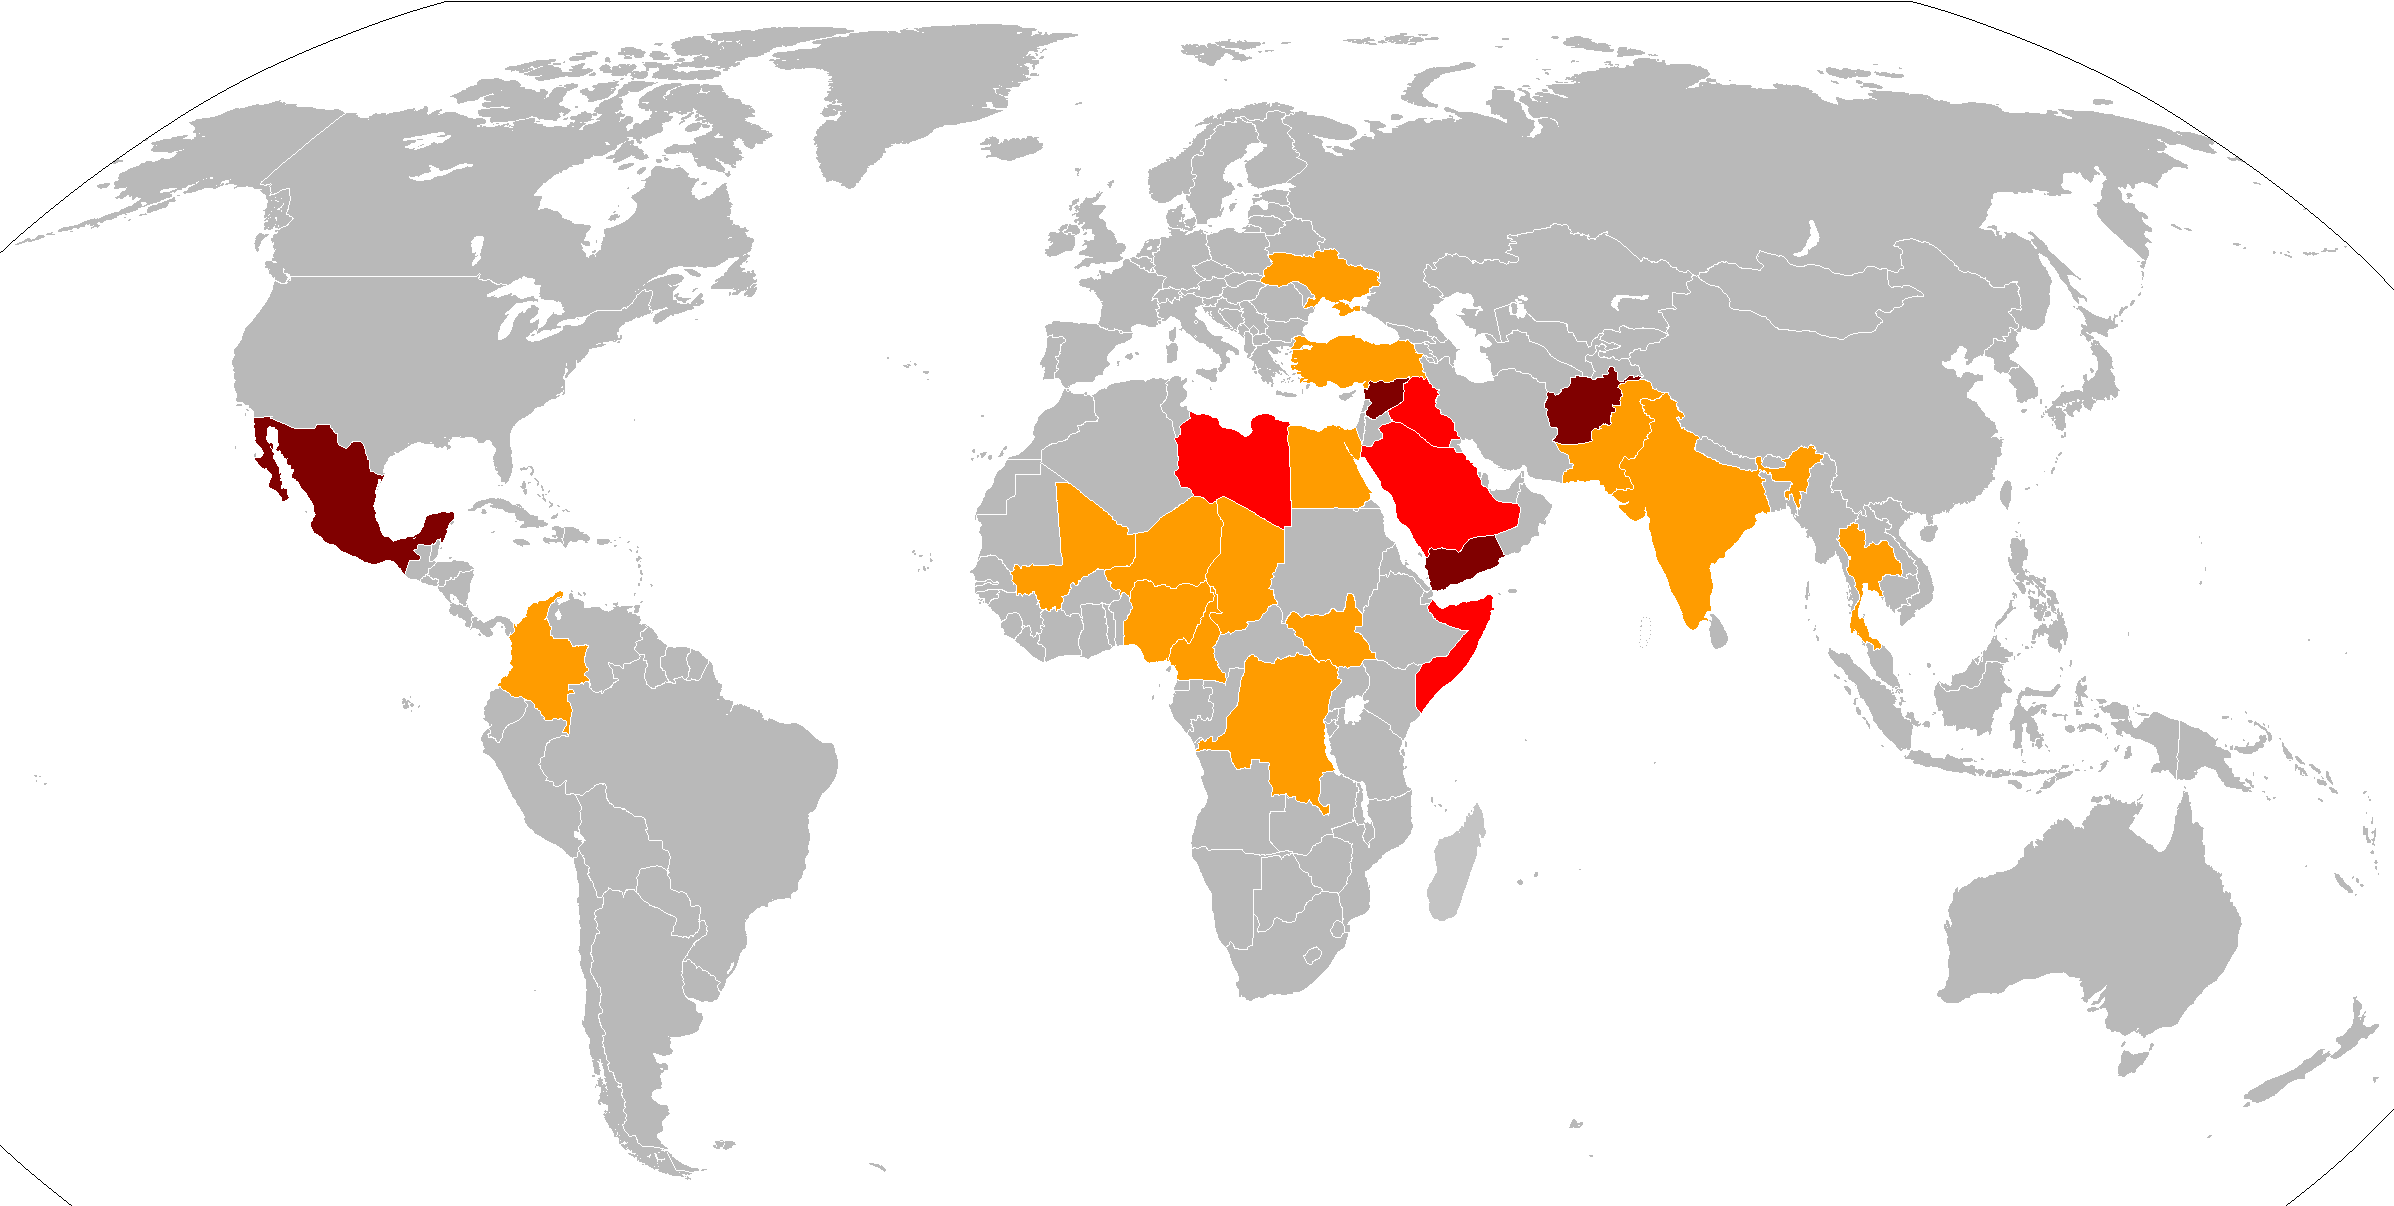
\includegraphics[width=17cm]{images/Libro-img033.png}
    \caption{Grandi guerre, 10.000 o più morti legate alla battaglia nell'anno corrente o passato\\
(rosso) Guerre, 1.000-9.999 morti legate alla battaglia nell'anno corrente o passato
(arancione) Conflitti meno intensi, 100-999 morti legate alla battaglia nell'anno corrente o passato
Credits: CC BY-SA 3.0, \protect\url{https://en.wikipedia.org/w/index.php?curid=63106445}  }
  \end{minipage}
\end{figure}

\begin{figure}[H]
  \begin{minipage}{17cm}
    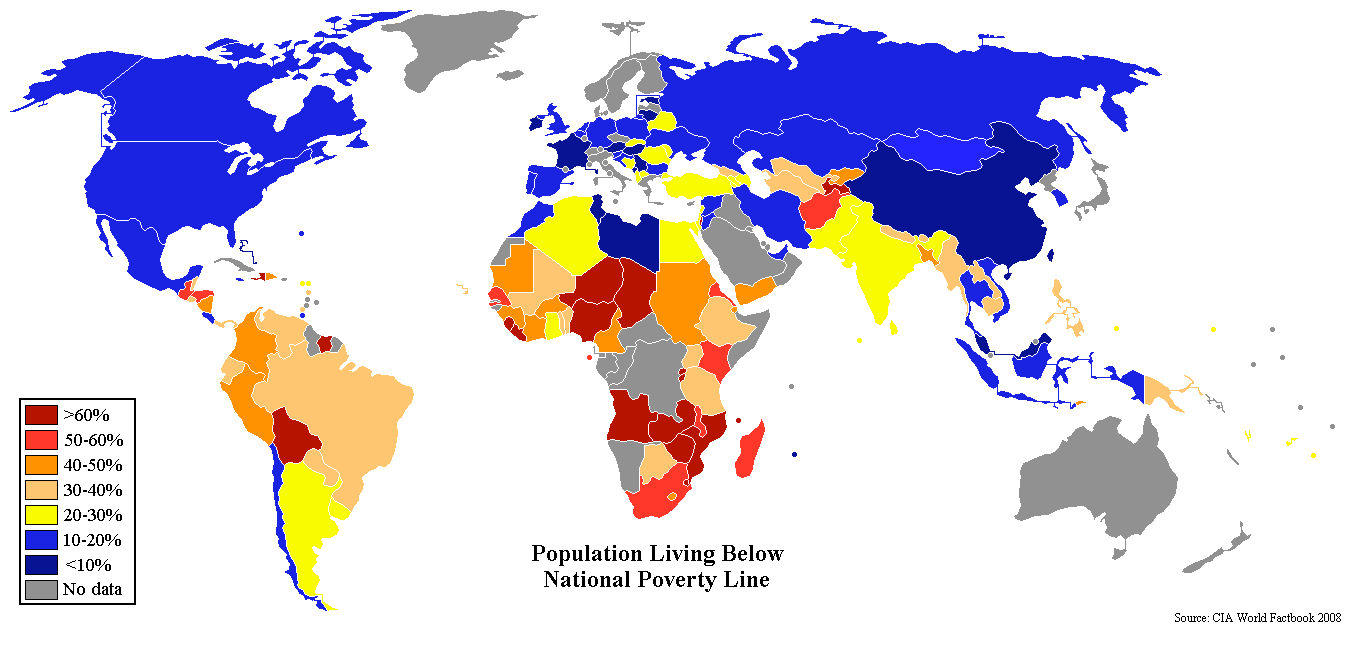
\includegraphics[width=17cm]{images/Libro-img034.png}
    \caption{Popolazione che vive al di sotto della soglia nazionale di povertà \\
Credits: Sbw01f - kaart armoedegrens [1], CC BY-SA 3.0, \protect\url{https://commons.wikimedia.org/w/index.php?curid=3730813}}
  \end{minipage}
\end{figure}

Tiziano Terzani in un intervista sull'undici settembre spiegava come la violenza genera altra
violenza, è un cliché forse ma è chiaro, lineare, comprensibile, non solo, a riprova di questo, ha detto una cosa
ancora più rivoluzionaria: la reazione avuta dagli americani l'ha paragonata a un “cancro curato
male”, che si diffonde poi in tutto il corpo. Io sono capitato su questa intervista quando è esploso il caso ISIS, anni
dopo la sua morte e, col senno di poi possiamo dire che ci avesse visto lungo.

Follia è fare sempre la stessa cosa e aspettare risultati diversi (Albert Einstein).

Secoli di guerra, carcere, pene di morte e detenzione di armi non hanno portato la pace

\begin{figure}[H]
  \begin{minipage}{17cm}
    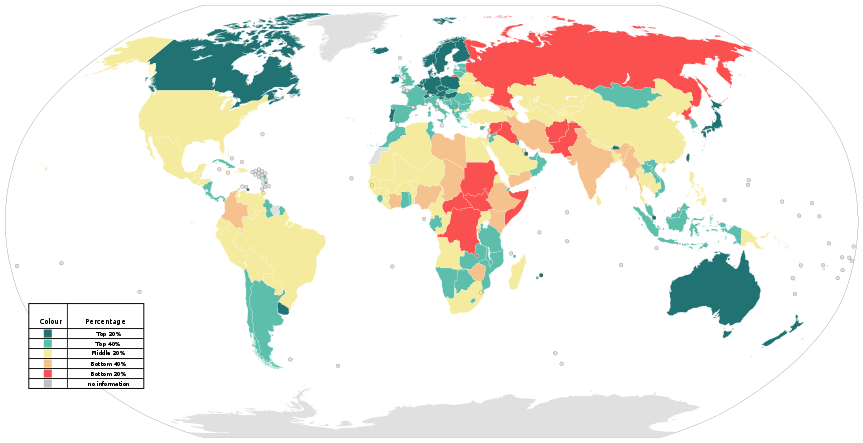
\includegraphics[width=17cm]{images/Libro-img035.png}
    \caption{GPI (Global Pace Index) o Indice della pace e della sicurezza mondiale. \\
In testa alla classifica dei paesi più pacifici: Islanda (1 GPI), Nuova Zelanda (2 GPI), Portogallo (3 GPI), Austria (4
GPI), Danimarca (5 GPI), Canada (6 GPI ), Singapore (7 GPI), Slovenia (8 GPI), Giappone (9 GPI), Svizzera (10 GPI). \\
In fondo alla classifica troviamo: Russia (154 GPI), Repubblica Democratica del Congo (155 GPI), Libia (156 GPI),
Repubblica Centrafricana (157 GPI), Afghanistan (158 GPI), Iraq (159 GPI), Yemen (160 GPI), Siria (161 GPI), Sudan del
Sud (162 GPI), Somalia (163 GPI).\\
L'Italia si trova 39° su 163\\
\protect\url{https://it.wikipedia.org/wiki/Global\_Peace\_Index} \\
Credits: Di Fedeeee03 - Opera propria, CC BY-SA 4.0, \protect\url{https://commons.wikimedia.org/w/index.php?curid=70198409}  }
  \end{minipage}
\end{figure}

\begin{figure}[H]
  \begin{minipage}{17cm}
    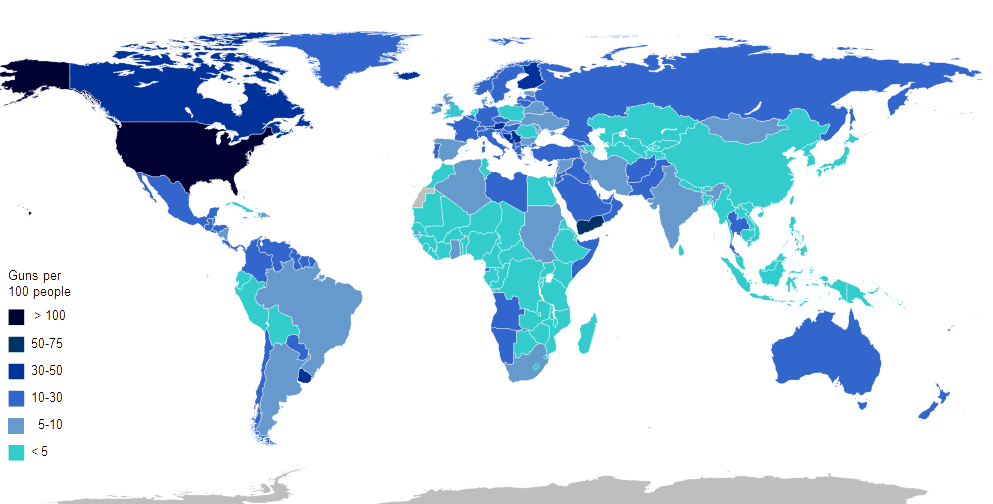
\includegraphics[width=17cm]{images/Libro-img036.png}
    \caption{Detenzione di armi di privati cittadini. Anche qua notiamo
come sia in cima che in fondo alla classifica troviamo paesi con GPI o indice di pace e sicurezza, di tutti i tipi, sia
valori buoni che scarsi. Questo vuol dire che pace e armi non vanno di pari passo, sono valori slegati.\\
I maggiori possessori di armi sono in ordine: Stati Uniti (128), Isole Malvine (N.D), Yemen (160), Nuova Caledonia
(N.D.), Montenegro (67), Serbia (50), Canada (6), Uruguay (34), Cipro (48), Finlandia (14). \\
In fondo alla classifica: Corea del nord (151), Malawi (38), Singapore (7), Timor Est (63), Corea del sud (55), Isole
Salomone (N.D.), Isola di natale (N.D.), Città del vaticano (N.D.), Indonesia (41), Nauru (N.D.), Taiwan (36)\\
L'Italia si trova 52° su 230\\
\protect\url{https://en.wikipedia.org/wiki/Estimated\_number\_of\_civilian\_guns\_per\_capita\_by\_country} \\
Credits: By RGloucester - This file was derived from: \ BlankMap-FlatWorld6.svgData from Small Arms Survey 2017 by the
the Graduate Institute of International and Development Studies in Geneva, Public Domain,
\protect\url{https://commons.wikimedia.org/w/index.php?curid=26085935} }
  \end{minipage}
\end{figure}

\begin{figure}[H]
  \begin{minipage}{17cm}
    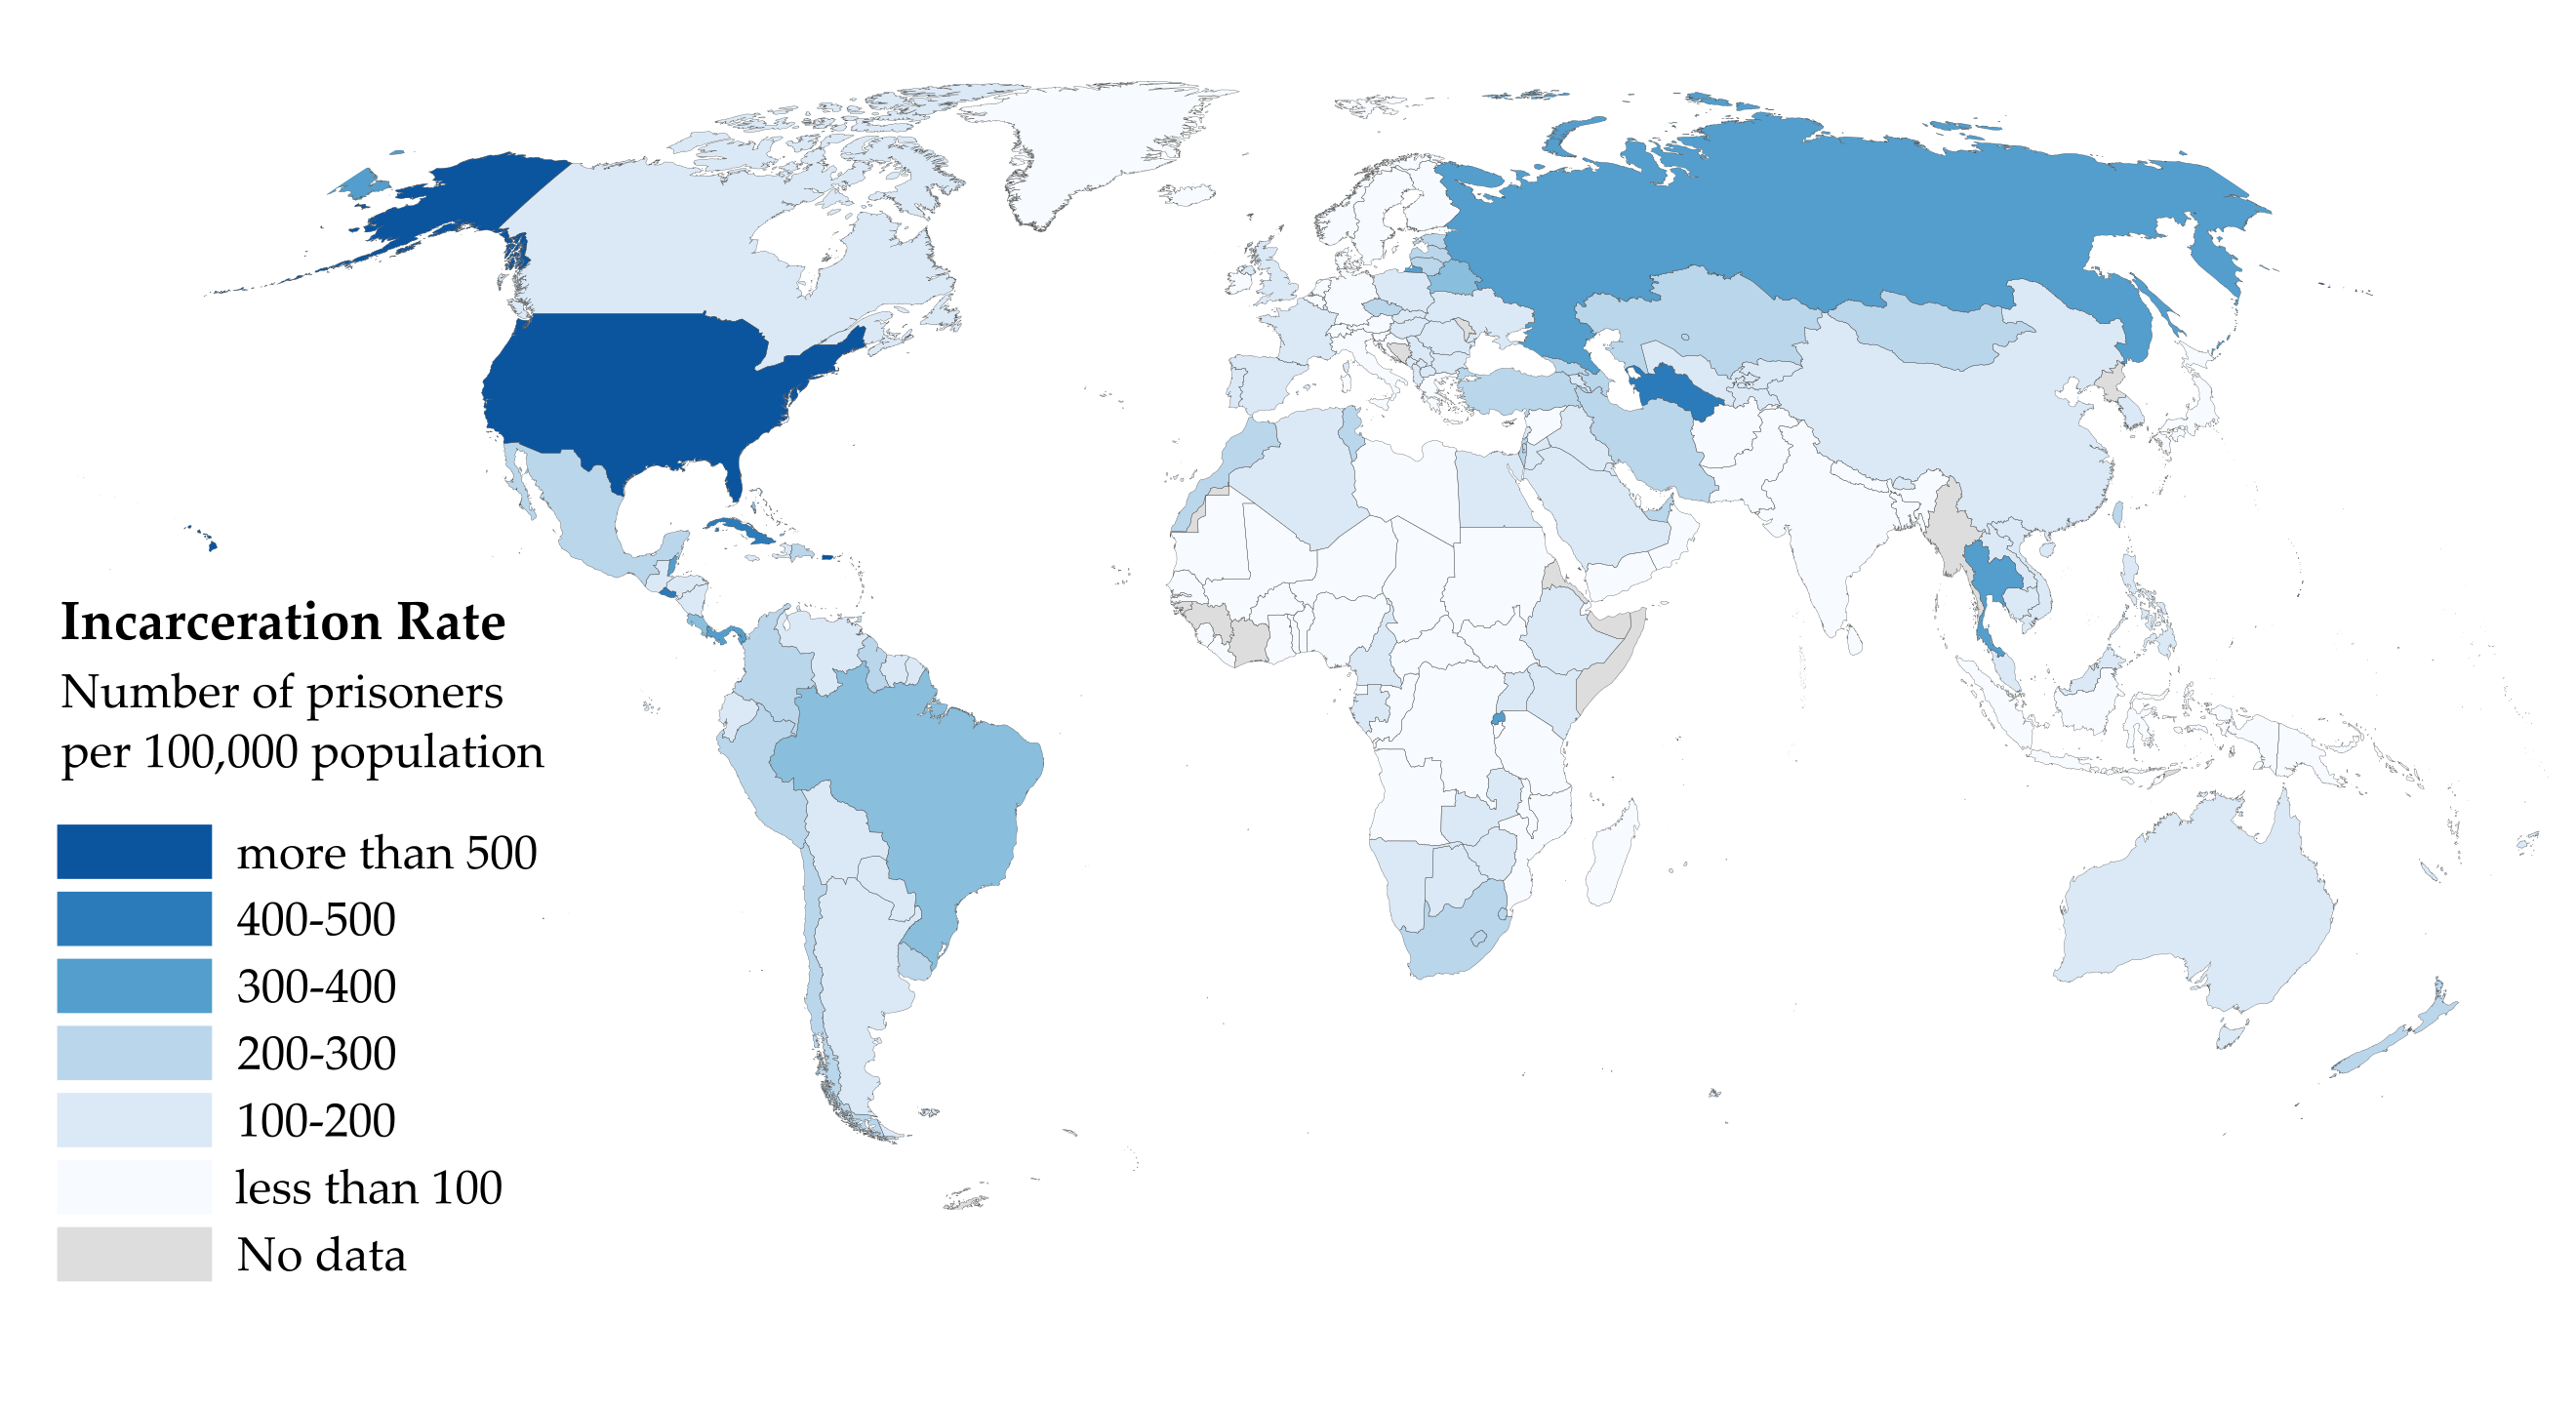
\includegraphics[width=17cm]{images/Libro-img037.png}
    \caption{Elenco dei paesi per tasso di detenzione. Notiamo come
sia in cima che in fondo alla classifica troviamo paesi con GPI o indice di pace e sicurezza, di tutti i tipi, sia
valori buoni che scarsi. Questo vuol dire che pace e carcere non vanno di pari passo.\\
In cima alla classifica, i paesi con meno detenuti: Afghanistan (158 GPI), Albania (51 GPI), Algeria (111 GPI), Samoa
(N.D. GPI), Andorra (N.D. GPI), Angola (77 GPI) , Anguilla (N.D. GPI), Antigua e Barbuda (N.D. GPI), Argentina (75
GPI), Armenia (118 GPI )\\
Infine i paesi con più detenuti: Stati Uniti (128 GPI), Uruguay (34 GPI), Uzbekistan (102 GPI), Vanuatu (N.D.),
Venezuela (144 GPI), Vietnam (57 GPI), Isole Vergini (Britanniche) (N.D. GPI), Isole Vergini (USA) (N.D. GPI), Yemen
(160 GPI), Zambia (49 GPI), Zimbabwe (132 GPI)\\
L'Italia si trova 99° su 223\\
\protect\url{https://en.wikipedia.org/wiki/List\_of\_countries\_by\_incarceration\_rate}\\
Credits: By Jannick88 - Own work, CC BY-SA 4.0, \protect\url{https://commons.wikimedia.org/w/index.php?curid=61711663} }
  \end{minipage}
\end{figure}

\begin{figure}[H]
  \begin{minipage}{17cm}
    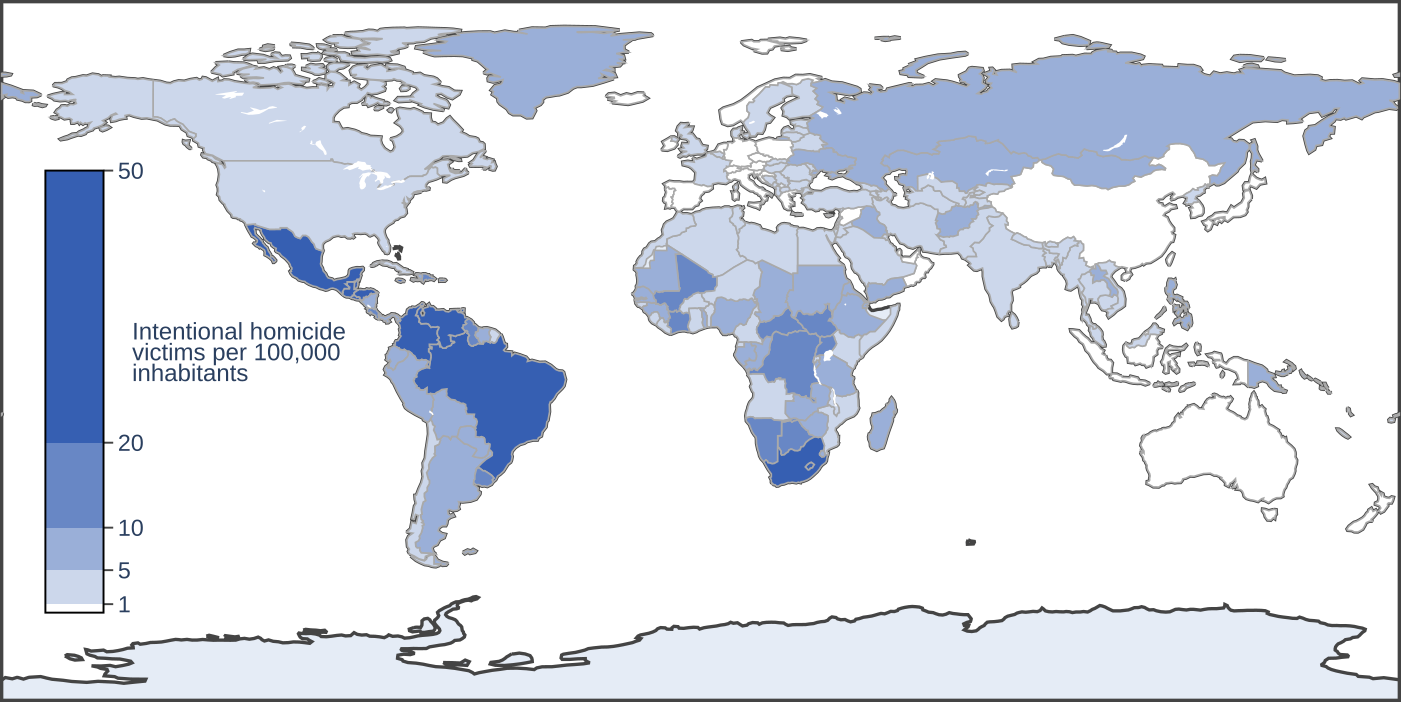
\includegraphics[width=17cm]{images/Libro-img038.png}
    \caption{Tasso di omicidi. Possiamo notare, confrontando questa
mappa con quella dei paesi per tasso di detenzione che non ci sono correlazioni tra aumento di pena e diminuzione di
reato. Anzi, troviamo una leggera correlazione del contrario.\\
In cima alla lista dei paesi con il più alto tasso di omicidio troviamo: El Salvador, Isole Vergini americane, Jamaica,
Lesotho, Honduras, Belize, Venezuela, Saint Vincent e Grenadines, Sud Africa, Saint Kitts e Nevis\\
Infine i paesi con meno omicidi: Giappone, Singapore, Sant'Elena, Channel Islands, Isle of Man,
Andorra, Città del Vaticano, San Marino, Monaco, Nauru, Niue\\
L'Italia si trova 206° su 230\\
\protect\url{https://en.wikipedia.org/wiki/List\_of\_countries\_by\_intentional\_homicide\_rate} \\
Credits: Iacopo Guarneri}
  \end{minipage}
\end{figure} 

Sia per la guerra che per il carcere una persona che ha tanto da perdere o comunque abbastanza da perdere, ovviamente
sarà più improbabile che delinquerà per qualcosa che comunque potrebbe ottenere anche se in più tempo. Il rapporto
rischi benefici è svantaggioso siccome il rischio è veramente alto e il beneficio può essere comunque ottenuto per
esempio risparmiando. Infatti la maggior parte dei reati sono quelli legati allo spaccio o piccoli furti, proprio per
sopperire alla mancanza di entrate economiche. Omicidi, reati associativi e traffico internazionale sono una minoranza,
circa il 10\%. Quindi la maggior parte dei carcerati sono poveri, tossici o stranieri, categorie che non possono
nemmeno sostenere economicamente un processo. Il carcere è comunque necessario per persone pericolose che se in libertà
possono nuocere alla vita o la sicurezza delle altre persone, non è utile per persone che sarebbero innocue se avessero
le condizioni necessarie per sopravvivere, il lavoro in primis. A riprova di quanto detto sappiamo che il \ Il 70\%
delle persone ritorna in
carcere\endnote{\protect\url{https://www.amazon.it/Abolire-carcere-ragionevole-sicurezza-cittadini-ebook/dp/B00VEALL62} }. Mentre se
si utilizzano misure alternative che non le dono la dignità, come affidamento, servizi sociali e domiciliari, il tasso
di recidività crolla al 20\%. Questo dato ci suggerisce due cose, la prima è che evidentemente non è servito, questa
persona non è stata “rieducata”. Il secondo punto suggerisce che probabilmente è stato tentato di risolvere il problema
solo all'ultimo strato superficiale e non sono stati risolti i motivi alla base che hanno portato
quella persona a delinquere. Spesso, se una persona ruba, è perché non ha soldi per mangiare, pagare
l'affitto, le bollette ecc… e fuori dal carcere si ritroverà nella stessa situazione, è probabile
che farà quello che è necessario per sopravvivere. Queste persone non sono state rieducate dal carcere proprio perché
sono già educate alla società, sono consapevoli di cosa si giusto e sbagliato e di quali azioni possono recare danno.
In carcere succede che le persone, oltre alla libertà, vengono privati di affetti e intimità, \ perché, siccome andare
a trovare un carcerato è piuttosto complicato, anche i parenti, iniziano a fargli visita sempre meno. Un individuo,
quando esce dal carcere, è incattivito contro questo Sistema e lo Stato, quindi farà più attenzione a non farsi
beccare, inoltre, siccome in questo lasso di tempo avrà conosciuto altre persone, delinquerà di più, perché avrà
imparato altri modi di delinquere. 


\bigskip
\begin{mdframed}[linewidth=1pt]
Avere un'arma in casa ci rende più sicuri?

No, secondo alcuni studi. Un'analisi di 15 diversi studi scientifici ha riscontrato che tenere in casa un'arma da fuoco
quasi raddoppiala probabilità di morire assassinati. Uno studio della Emory
University\endnote{\protect\url{https://journals.lww.com/jtrauma/Abstract/1998/08000/Injuries\_and\_Deaths\_Due\_to\_Firearms\_in\_the\_Home.10.aspx}
} su 626 casi di sparo avvenuti in casa in tre città Usa (Memphis, Seattle e Galveston), dimostra che sono quattro
volte più frequenti gli spari accidentali che per autodifesa e sette volte superiori quelli per compiere un aggressione
o un omicidio e infine undici volte in più i colpi per suicidio. Secondo il Injury Control Research Center di Harvard
le armi sono usate per autodifesa in meno dell'1\% delle aggressioni con una vittima. Secondo John Donohue, economista
della Stanford University, 2017, quando uno Stato riduce i requisiti per il porto d'armi, cresce il numero di crimini
violenti.
\end{mdframed}

\bigskip

Ma l'alternativa qual è? Poi non possiamo fare di tutta l'erba un fascio,
siamo sette miliardi, per cui ci sarà sempre una piccola porzione di società, dove anche con le condizioni necessarie
alla sopravvivenza per avidità troveranno nella criminalità una via facile ai loro scopi. In ogni caso, se una persona
delinque è giusto che paghi, ma non con la sua libertà, a meno di persone davvero pericolose per gli altri. Una persona
che commette un reato economico deve essere punita economicamente, non con la libertà. Inoltre risulta più efficace,
premiare i cooperatori più che punire i trasgressori, anche se entrambe le strategie possono coesistere, si potrebbe
pensare ad un modo per premiare le persone oneste in modo che un delinquente possa essere più incentivato in questa
direzione. Ogni anno le carceri costano tre miliardi di cui il 70\% va al personale interno e il 2\% a realtà esterne,
assistenti sociali ecc... Chi esce con l'indulto invece ha meno possibilità di entrare nuovamente in carcere, questo
deve far pensare. Se si depenalizzassero le droghe leggere, la popolazione carceraria crollerebbe perché la maggioranza
sono dentro per spaccio. Questo porterebbe ad avere meno processi e quindi una giurisdizione più veloce ed efficiente,
ma anche più soldi da impegnare in attività di recupero del carcerato. Il Portogallo ad esempio ha depenalizzato il
consumo di tutte le droghe nel 2001, sia leggere che non e, con risultati ottimi: Secondo un rapporto del 2017
dell'Institute of Labor
Economics\endnote{\protect\url{https://www.iza.org/publications/dp/10895/going-after-the-addiction-not-the-addicted-the-impact-of-drug-decriminalization-in-portugal\#:\~{}:text=The\%20results\%20suggest\%20that\%20a,number\%20of\%20clients\%20entering\%20treatment.}
}, la depenalizzazione “ha contribuito a un calo nel numero di sequestri di eroina e cocaina, una diminuzione del
numero di reati e decessi per droga e una diminuzione del numero di pazienti che entrano in cura”. 

Possiamo trasformare la popolazione carceraria da costo a risorsa impiegandola in lavori socialmente utili, e in
aziende, artigiani, contadini che hanno un esubero di lavoro legato alla stagionalità per esempio. In questo modo
vengono realmente introdotti e non isolati dalla società, imparano un mestiere, iniziano a conoscere persone che
possono dare loro una mano. Quando noi andiamo a cercare un lavoro chi viene chiesto quali sono state le nostre
esperienze lavorative negli ultimi anni trascorsi, dire “nessuna” o peggio ancora “sono stato in carcere” equivale a
essere scartati. Anche qua, uno può veramente provarci a cambiare vita, ma con possibilità così basse di trovare lavoro
e di conseguenza senza entrate economiche, quanto puoi resistere? Inoltre il carcere è un ambiente dove sei circondato
da violenza e, a subirla, da parte degli altri carcerati e dalle guardie. Quanto è probabile che porgerai sempre
l'altra guancia o che a un certo punto inizierai a reagire quotidianamente da farlo diventare
normale? questo come può farti diventare una persona migliore? 

Riporto sempre il discorso al lavoro perché penso che sia proprio questa la chiave. Se in un mondo ipotetico ogni
persona avesse soldi infiniti nessuno delinquerebbe, quindi a mio avviso è direttamente proporzionale la criminalità
con le entrate economiche e, quest'ultima è legata al lavoro che è legata
all'istruzione. I dati infatti ci dicono esserci una relazione tra delinquenza ed
istruzione\endnote{\protect\url{https://italiaindati.com/carceri-in-italia/} }.


\bigskip
\begin{mdframed}[linewidth=1pt]
La caccia è utile?

La caccia, inizialmente nata con l'obiettivo della sopravvivenza è diventata ai giorni nostri uno
strumento per controllare che una specie animale non diventi troppo presente e, anche, per fini ludici. Gli animalisti
da anni sii battono contro questa pratica, ma se sparisse, il numero di certi animali crescerebbe fuori controllo? In
Italia, uno degli animali che crea più preoccupazione sotto questo punto di vista è sicuramente il cinghiale. Secondo
dati ISPRA (Istituto superiore per la protezione e la ricerca ambientale) i cinghiali sono raddoppiati in 10 anni,
passando da 500 mila del 2010 a 1 milione nel 2020 nonostante il numero dei cacciatori sia stabile dal
1980\endnote{\protect\url{https://www.researchgate.net/publication/269636662\_Wild\_boar\_populations\_up\_numbers\_of\_hunters\_down\_A\_review\_of\_trends\_and\_implications\_for\_Europe}
}. Com'è possibile? Non può essere che l'uccisione dei cinghiali ne faccia
aumentare il numero. Sul breve periodo il numero diminuisce ma sul lungo periodo, al contrario, aumenta.

Il cinghiale vive in gruppi familiari matriarcali guidati da una vecchia femmina, chiamata matrona, che vive in un
territorio più ampio di un grande maschio dominante detto salengano. In condizioni normali sono solo la femmina e il
maschio dominante a riprodursi e, data l'età avanzata dei genitori, la prole non è abbondante.
Queste condizioni normali vengono alterate dalla caccia, siccome le matrone e il salengano sono i primi a morire in
quanto impegnati a far scappare giovani e cuccioli. In questo modo l'ordine gerarchico si spezza e
tutti i maschi vengono liberati dal controllo del dominante che gli impediva di riprodursi. Inizia così una fase
riproduttiva intensa, che vista la giovane età moltiplica rapidamente la popolazione con figliate di anche 12, 13
cuccioli. \ A confermarlo indirettamente sono gli stessi cacciatori, che tra le regole stilate e che normano la
cosiddetta “caccia di selezione” c'è una logica piramidale che prevede di uccidere in misura maggiore gli individui più
anziani e in misura minore i giovani e cuccioli, svecchiando così la popolazione di ungulati, lasciando in maggioranza
la fascia di età più fertile\endnote{\protect\url{https://www.fondazioneuna.org/news/guida-alla-caccia-di-selezione/} \ }.

Se cerchiamo su Google: “cinghiale caccia ricerche scientifiche” possiamo accorgerci di quante siano le ricerche
scientifiche che dimostrano che la caccia, oltre a non essere la soluzione, è parte del problema. Io ho trovato 26
studi\endnote{\par 1) Apollonio M., R. Putman, S. Grignolio \& L. Bartoš 2011. Hunting seasons in relation to
biological breeding seasons and the implications for the control or regulation of ungulate populations. In: M.
Apollonio, R. Andersen \& R. Putman (eds.), Ungulate management in Europe: Problems and practices, Cambridge University
Press, London, UK: 80-105.\par 2) Cahill S. \& D. Llimona 2004. Demographics of a wild boar Sus scrofa Linnaeus, 1758
population on a metropolitan park in Barcelona. In: C. Fonseca, J. Herrero, A. Luís \& A. M. V. M. Soares (eds.), Wild
boar research 2002, 4th International wild boar symposium, Galemys, 16 (n° especial): 37-52.\par 3) Canu A., Scandura,
E. Merli, R. Chirichella, E. Bottero, F. Chianucci, A. Cutini \& M. Apollonio 2015. Reproductive phenology and
conception synchrony in a natural wild boar population. Hystrix 26 (2): 77-84.\par 4) Dardaillon M. 1988. Wild boar
social groupings and their seasonal changes in the Camargue, southern France. Z. Säugetierkunde 53: 22-30.\par 5)
Delcroix I., R. Mauget \& J. P. Signoret 1990. Existence of synchronization of reproduction at the level of the social
group of the European wild boar (Sus scrofa). J. Repr. Fert. 89: 613-617.\par 6) Eisenberg J. F. \& M. Lockhart 1972.
An ecological reconnaisance of Wilpattu National Park, Ceylon. Smithsonian Inst. Press, Washington, D. C.\par 7)
Gamelon M., A. Besnard, J.-M. Gaillard, S. Servanty, E. Baubet, S. Brandt \& O. Gimenez 2011. High hunting pressure
selects for earlier birth date: wild boar as a case study. Evolution 65 (11): 3100-3112.\par 8) Gayet T., S. Devillard,
M. Gamelon, S. Brandt, L. Say \& E. Baubet 2016. On the evolutionary consequences of increasing litter size with
multiple paternity in wild boar (Sus scrofa scrofa). Evolution 70 (6): 1386–1397.\par 9) Graves H. B. 1984. Behaviour
and Ecology of Wild and Feral Swine (Sus scrofa). Journal of Animal Science 58 (2): 482–492.\par 10) Herrero J., A.
García-Serrano \& R. García-Gonzalez, 2008. Reproductive and demographic parameters in two Iberian wild boar Sus scrofa
populations. Acta theriologica 53 (4): 355-364.\par 11) Istituto nazionale per la fauna selvatica (2002). Gli Ungulati
in Italia. Status, distribuzione, consistenza, gestione e prelievo venatorio. Istituto nazionale per la fauna selvatica
“Alessandro Chigi”, 61 pp.\par 12) Ježek M. 2012. The influence of sex mature of wild boar to reproduction in the Czech
republic. Vliv pohlavního dospívání na reprodukci prasete divokého v České Republice. Doctoral thesis. Disertační
práce. Praha, 72 pp.\par 13) Kaminski G., S. Brandt, E. Baubet \& C. Baudoin 2005. Life-history patterns in female wild
boars (Sus scrofa): mother-daughter postweaning associations. Canadian Journal of Zoology 83: 474-480.\par 14) Marsan
A., L. Schenone \& S. Spanò 2000. Il cinghiale in Liguria. II edizione. Regione Liguria, Struttura allevamento, caccia
e pesca, 103 pp., 4 tavv.\par 15) Marsan A., S. Spanò \& C. Tognoni 1995. Management attempts of wild boar (Sus scrofa
scrofa L.): first results and ongoing researches in Northern Apennines. Ibex 3: 219-221.\par 16) Massei G., J.
Kindberg, A. Licoppe, D. Gačić, N. Šprem, J. Kamler, E. Baubet, U. Hohmann, A. Monaco, J. Ozoliņš, S. Cellina, T.
Podgórski, C. Fonseca, N. Markov, B. Pokorny, C. Rosell \& A. Náhlik 2015. Wild boar populations up, numbers of hunters
down? A review of trends and implications for Europe. Pest Management Science 71 (4): 492-500.\par 17) Mauget R. 1982.
Seasonality of reproduction in the wild boar. In: D. J. A. Cole \& G. R. Foxcroft (eds.), Control of pig reproduction,
Butterworth, London: 509–526.\par 18) Mazzoni della Stella R., F. Calovi \& L. Burrini 1995. The wild boar management
in a province of the Central Italy. Ibex 3: 213-216.\par 19) Meynhardt H. 1986. Schwarzwild-Report. Mein Leben unter
Wildschweinen. Naumann, Leipzig, 223 pp.\par 20) Moretti M. 1995. Birth distribution, structure and dynamics of a
hunted mountain population of wild boars (Sus scrofa L.), Ticino, Switzerland. Ibex 3: 192-196.\par 21) Oliver W. \& K.
Leus 2011. Sus scrofa. IUCN Red List of threatened species, version 2011.2, 6 pp.\par 22) Scillitani L., A. Monaco \&
S. Toso 2010. Do intensive drive hunts affect wild boar (Sus scrofa) spatial behaviour in Italy? Some evidences and
management implications. European Journal of Wildlife Research 56 (3): 307–318.\par 23) Servanty S., J.-M. Gaillard, C.
Toïgo, S. Brandt \& E. Baubet 2009. Pulsed resources and climate-induced variation in the reproductive traits of wild
boar under high hunting pressure. J. animal ecology 78 (6): 1278-1290.\par 24) Thurfjell H., G. Spong \& G. Ericsson
2013. Effects of hunting on wild boar Sus scrofa behaviour. Wildlife Biology 19 (1): 87-93.\par 25) Toïgo C., S.
Servanty, J.-M. Gaillard, S. Brandt \& E. Baubet 2008. Disentangling natural from hunting mortality in an intensively
hunted wild boar population. J. Wildlife Management 72 (7): 1532-1539.\par 26) Scillitani L., A. Monaco \& S. Toso
2010. Do intensive drive hunts affect wild boar (Sus scrofa) spatial behaviour in Italy? Some evidences and management
implications. European Journal of Wildlife Research 56 (3): 307–318. }. Ho provato a cercare studi che sostenessero la
tesi opposta, ma l'unico che ho trovato, sostiene che la caccia e i cacciatori siano utili per i
censimenti, ma non per il contenimento del numero. 

Indipendentemente dalle ricerche, anche a livello intuitivo, se la caccia funzionasse, dopo tutti questi anni il
problema dovrebbe essersi risolto o almeno essere in una fase di decrescita e, invece è l'esatto
opposto. Quello che ne resta è lo scopo ludico che potrebbe anche starci, ma il solo divertimento, a fronte di un danno
ambientale così importante non è più giustificabile. Immagino sia stimolante seguire le tracce, stanare la preda, ma è
possibile farlo anche senza un fucile, tanti, con l'aumento di popolarità della fotografia,
preferiscono questa modalità per non rinunciare all'aspetto ludico.

Quindi quali soluzioni ci possono essere? Come spesso accade in questi casi, la natura ha una forte capacità di
ritrovare un suo equilibrio in maniera autonoma. In Italia negli ultimi anni si sta assistendo a una ricomparsa del
lupo, unico predatore dei grandi ungulati presenti sul territorio. Possiamo trovare un virtuoso esempio del Parco
Nazionale del Gran Paradiso che sta reintroducendo il lupo proprio per la sua azione predatoria utile nel controllo
numerico dei cinghiali. Uno dei problemi che ha portato alla crescita esponenziale dei cinghiali è stata proprio la
caccia spietata del lupo in passato che l'ha quasi portata alla sua estinzione.
Tutt'ora, controllare il numero dei lupi risulta controproducente. I branchi di lupi sottoposti a
\ pressione venatoria si disperdono, così i singoli individui, senza l'appoggio degli altri
esemplari, non sono più in grado di cacciare prede selvatiche e si rivolgeranno alle più facili prede domestiche, dalle
pecore ai piccoli cani. Non ci sono mai troppi carnivori nell'equilibrio della natura, ce ne sono
tanti quanti la catena alimentare ne consente.

Sembra che la legge in questo ambito sia orientata a tutelare l'attività venatoria più che
l'equilibrio naturale, infatti, gli agricoltori, se cacciatori, possono abbattere animali sorpresi
nei loro campi per tutto l'anno, anche fuori i periodi di caccia, ma non hanno
l'obbligo di creare recinti elettrificati (disposti in maniera corretta) che si sono dimostrati
negli anni molto efficaci per la protezione del bestiame. Le misure di controllo del bestiame, come recinti e cani
pastore, risultano necessarie in ogni caso, anche se si riuscisse ad uccidere ogni lupo presente sul territorio. Una
ricerca del wwf condotta in Svizzera ha riportato che i lupi ogni uccidono circa 200 esemplari. In confronto, ogni
estate negli alpeggi muoiono per malattia o cadute dai precipizi circa 4000 pecore perché non sufficientemente
sorvegliate. Anche i dissuasori elettronici, lungo le strade boschive hanno dimostrato la loro efficacia nella
riduzione degli incidenti stradali.

La vera paura però, non è quella che il lupo attacchi il bestiame, ma che attacchi l'uomo. Il lupo
però è un animale schivo e ha paura dell'uomo. L'ultimo attacco ad una
persona, da parte di un lupo infatti risale al 1800. Molte più vittime dipendono dalla caccia in sé. Dal 2011 al 2021
(con una pandemia di mezzo che ha ridotto l'attività venatoria), i morti umani per colpa della
caccia sono stati 209 con 682 i feriti, questo è ciò che emerge dai dati raccolti da vittimedellacaccia.org. La
maggioranza delle vittime sono stati cacciatori, ma ci sono stati casi di gente che stava passeggiando nei boschi e
addirittura persone colpite mentre erano dentro casa loro. 
\end{mdframed}

\subsection{Lavoro e scuola}
Il problema alla base che va risolto quindi è il lavoro, dove in casi estremi, come paesi colpiti dalla guerra, va
proprio costruito tutto da zero, mentre in occidente, siamo portati a dire che, per colpa dello Stato non
c'è lavoro. Qua potrei scatenare le ire di qualcuno, premetto che il mio discorso non è assoluto
ma relativo ad alcuni casi, sicuramente lo stato può fare tanto, ma anche le persone! Sarebbe bello vivere in un posto
dove ci DEVONO dare il lavoro, ma la verità è che nulla ci è dovuto. Dobbiamo noi stessi investire sulla nostra
professionalità, se non sappiamo fare niente, perché qualcuno dovrebbe volerci assumere? Non dico che dobbiamo
diventare tutti dei fisici aerospaziali, ma se uno entra in un'azienda edile e studia per prendere
brevetti o patenti per guidare la ruspa, il camion, la gru ecc… eserciterà sicuramente una leva più vantaggiosa sul suo
futuro lavorativo rispetto ad altri. Dalla criminalità siamo arrivati al lavoro come soluzione e per il problema del
lavoro possiamo arrivare alla scuola e al fattore culturale. La scuola potrebbe fare molto in questo senso invece si
limita a darti delle nozioni e, non degli strumenti molte volte. I ragazzi che oggi stanno frequentando scuola, saranno
i lavoratori del futuro, dove, ci saranno lavori che oggi ancora non esistono e le cui nozioni che possiamo offrire
saranno inutili. Questo fenomeno sarà sempre più frequente in un mondo che cambia così velocemente e, sarà quindi
impensabile credere di non studiare più a scuola finita. Per questo motivo più che le nozioni la scuola dovrebbe in
primis insegnare a pensare, imparare a imparare, la gestione del tempo, risolvere problemi, la gestione interpersonale
ecc… Edgar Morin diceva: “E' meglio una testa ben fatta che una testa ben piena”.

\begin{itemize}
\item Problem solving (risoluzione dei problemi): Una concezione molto comune dell'ambiente
scolastico è quella di giustificare una mancata consegna di un lavoro con frasi tipo: non lo sapevo fare, non me
l'hanno detto, non ci sono riuscito ecc… Chi ripropone questo schema sul posto di lavoro si
troverà spesso in lavori precari di pochi mesi che non verranno poi rinnovati. Quello che dovrebbero insegnare a scuola
ma anche in famiglia è che il datore di lavoro vuole sapere che se c'è un compito e lo da a te, tu
lo ricontatterai solo per dire che il lavoro è stato portato a termine, o come sta procedendo in casi di lavoro lunghi.
Non gli interessa sapere che problematiche stai riscontrando e che avresti bisogno di una mano per risolverle. Una
volta usciti dalle superiori o dall'università, anche se troviamo un posto di lavoro coerente con
quello che abbiamo studiato, non possiamo pensare che ci verranno assegnati solo lavori che sappiamo fare, anzi, più
siamo qualificati più ci verranno assegnati lavori che non sappiamo fare. La scuola ci deve fornire gli strumenti per
arrivare alla soluzione di problemi nuovi, non importa come, utilizzando documentazioni, manuali, facendo prove,
chiedendo aiuto a un collega o su Google, l'importante è che se ti viene assegnato un compito tu
in qualche modo lo porti a termine. Quello che è importante imparare è il metodo del problem solving che propone
diverse strategie come la scomposizione (prendere un macro problema e dividerlo in sottoproblemi più piccoli), trovare
i pattern (o schermi ricorrenti che tendono a presentarsi spesso in modo da poter creare uno strumento risolutivo
riutilizzabile in varie situazioni), astrazione (per individuare le caratteristiche principali di un problema
escludendo il superfluo che può invece sembrare significativo portandovi fuori strada), la generalizzazione (utile a
tradurre un problema in un altro che già conosciamo e sappiamo risolvere) e, la creazione di algoritmi, flow chart o
diagrammi di flusso per creare istruzioni efficaci alla soluzione di un problema.

\begin{mdframed}[linewidth=1pt]
A volte per risolvere un problema basta aggiungere variabili, anche a caso. Alcune volte abbiamo le soluzioni ai nostri
problemi al mattino, appena svegli, perché nel sonno la nostra testa fa associazioni che la nostra mente razionali non
farebbe mai. Quasi tutte le invenzioni sono l'unione di più cose, come ad esempio una carrozza più
la “variabile” motore, hanno generato l'automobile. Anche la genetica funziona in modo simile,
ogni individuo di una specie sarà diverso, uno avrà la pelliccia di un colore più chiaro, un altro il collo più lungo,
le orecchie più grandi e così via. La genetica aggiunge variabili con queste mutazioni per risolvere il problema della
sopravvivenza. Se questa mutazione è utile, l'individuo avrà più possibilità di sopravvivere e, la
sua prole, potrebbe manifestare la stessa mutazione e aggiungerne di nuove, migliorando sempre di più la soluzione al
problema della sopravvivenza. 

A questo proposito mi viene in mente la storia dell'ape e della mosca. Se si mette in una bottiglia
aperta una mosca e un ape, quest'ultima, siccome più intelligente, seguirà la luce e riuscirà ad
uscire, mentre la mosca inizierà a sbattere a destra e sinistra sulle pareti di vetro e con un po' di fortuna, a caso,
dopo un po' di tempo scapperà anche lei. Se rifacciamo la stessa cosa, girando sottosopra la
bottiglia, l'ape continuerà a seguire la luce ma questa volta sbatterà sul fondo della bottiglia e
morirà nel tentativo di scappare. La mosca, invece, seppur meno intelligente, facendo tentativi sempre nuovi, sempre
diversi, prima o poi riuscirà ad evadere. \newline
Altre volte per risolvere un problema basta distrarsi o dormirci su. Se abbiamo speso ore concentrandoci nella
risoluzione di un problema, la nostra mente focalizzerà l'attenzione su quello. Quando dormiamo la
nostra parte razionale rallenta e il cervello può slegarsi per pensare a soluzioni creative, aggiungendo variabili ce
nonavresti mai pensato da sveglio. Anche pensare ad altro può aiutare, fare una doccia o una passeggiata. La nostra
mente conscia, penserà ad altro ma il ostro cervello continuerà a cercare una soluzione senza che ci rendiamo conto. La
teoria dell'attrazione funziona su questo principio. Questa teoria dice che se desideri qualcosa
l'universo si organizzerà per dartela, in realtà se sei focalizzato su un certo obiettivo, la tua
mente, guarderà ogni cosa ordinaria, che ti capita nella giornata, sotto quest'ottica, al
raggiungimento di questo fine. Quindi la tua testa in ogni cosa che succede, cerca di prendere spunti o vedere
strumenti e risorse al proprio scopo, tanto che sembrano messe lì apposta certe occasioni, invece sei solo tu che le
vedi opportunità anche dopo apparentemente non ci sono. Sei più creativo nel cambiare una situazione a tuo favore
vedendo uno spiraglio verso la soluzione del tuo problema. Un certo avvenimento, che normalmente non avresti
considerato, la tua mente saprà trovarci un opportunità.
\end{mdframed}
\item Time management (gestione del tempo): In questo campo la scuola lo richiede ma non lo insegna. Infatti i compiti
scritti, compiti a casa, progetti di gruppo ecc… hanno tutti una data o ora di consegna che va rispettata e, qualcuno
trova dentro di se dei metodi per autogestirsi altri no. Esistono numerosi metodi, partendo da come imparare a stimare
e pianificare le varie mansioni e le loro tempistiche e, la tecnologia ci viene in contro con le todo list o lista
delle cose da fare con le varie deadline o scadenze. Sarebbe interessante approfondire tutti questi punti ma, se lo
trovate interessante vi invito a cercare dei libri che possono spiegare questi concetti sicuramente meglio di come
potrei farlo io.
\item Rapporti interpersonali: Su questo punto, ancora più dei precedenti ci sarebbe da scrivere. Molto spesso per
portare avanti un lavoro abbiamo bisogno della collaborazione degli altri.È fondamentale interpretare i feedback della
nostra comunicazione per comprendere i momenti in cui potremmo essere troppo invadenti. Dobbiamo evitare di parlare
sopra agli altri, cercare di competere o di avere sempre ragione. Inoltre, è importante non dare consigli non richiesti
e non cercare di far sembrare di sapere tutto. La metacomunicazione può essere uno strumento utile per discutere
apertamente della conversazione stessa, ad esempio, facendo presente se i toni si stanno alzando o se si sta creando
una sorta di competizione. È importante però tenere presente che queste riflessioni potrebbero causare fastidio o
rabbia in alcuni casi. Su questo punto in particolare ci sono delle linee guida generiche ma poi ognuno deve trovare
quello che funziona meglio per lui, il modo migliore per chiedere le cose e relazionarsi coi colleghi.
\item Renditi indispensabile: Un altro retaggio del mondo scolastico è pensare che tutto ti sia dovuto. Mostrati
propositivo e non aspettare che un superiore venga a dirti cosa dovresti fare ora. Ci sono persone con un insana
ambizione che per prendere il proprio spazio devono mettere i piedi in testa agli altri, sicuramente funziona e,
leggendo le biografie e le storie di grandi aziende l'hanno fatto più o meno tutti, ma credo che
prendere il proprio spazio senza prevaricare sugli altri vi renderà sempre una persona decorosa ed elegante. Ci sarà
una differenza tra un essere umano e un essere, no? Cos'è l'Umanità con la U
maiuscola se ci mettiamo i pedi in testa per una posizione più alta nell'organico?\newline
Non cercare di diventare un uomo di successo, ma piuttosto un uomo di valore (Albert Einstein).
\end{itemize}

\bigskip

In Italia ad esempio, abbiamo un basso livello di comprensione del testo ed è tramite questa capacità che possiamo
apprendere nuove cose. Questo significa che una volta finita la scuola che ci dava le nozioni, anche noi con lei,
abbiamo finito di apprendere. Roger Schank propone di insegnare alle persone a pensare, \ lavorando quindi su tutti i
processi cognitivi che offrono gli strumenti per imparare. Dividendoli in: processi concettuali (predirre,
modellizzare, sperimentare, valutare), processi analitici (diagnosticare, pianificare, determinare la cause,
giudicare), processi sociali (influenzare, lavorare in gruppo, negoziare, descrizione). Quindi passare da conoscenze e
nozioni a processi cognitivi. Schank afferma che non ha senso insegnare matematica, fisica, chimica, storia, italiano,
geografia se i ragazzi non ne vedono l'utilità e non possono fare dei collegamenti di impiego di
queste conoscenze nella vita privata o lavorativa. Semplicemente si limiteranno a memorizzarli e ripeterli, per passare
la verifica o l'interrogazione e subito dopo inizieranno a dimenticarli. Se i ragazzi non vedono
un utilità nel futuro, la vedranno solo nel presente, ovvero, essere promossi, in quanto vedono il concetto appena
imparato come fine a un bel voto più che a uno strumento che gli servirà nel lavoro o nella vita in generale.
Sicuramente la storia, la geografia, la letteratura sono cose importanti ma se non vengono ricordate il tempo impiegato
a insegnarle sarà stato perduto. Quindi meglio concentrare le proprie energie per assicurarsi che tutti sappiano bene
parlare e scrivere, piuttosto che essere stati in classe con la testa altrove mentre parlavano dei promessi sposi, la
divina commedia e fare temi pieni di errori. Concentrarsi sulla storia recente per capire perché alcune soluzioni ai
problemi, che vengono naturali e che sembrano logicamente funzionanti sono già state provate e hanno fallito, quindi
approfittare di quel tempo per sforzare il pensiero e fare un dibattito delle possibili alternative. Invece che avere
persone che hanno visto un po' di logaritmi, un po' di studio di funzioni assicurarsi che tutti
abbiano le competenze di algebra base per risolvere i problemi di tutti i giorni. Forse dirò una cosa impopolare e,
seppur andassi bene in matematica, credo che la maggioranza delle persone non utilizzerà mai gli integrali e le
derivate, mentre le equazioni di primo grado si anche se tanti adulti non le sanno fare. Anche se nelle scuole
insegniamo la letteratura, la storia e l'arte avremo adulti a cui non importa nulla di tutto
questo e non ne avranno alcun interesse e, vivono bene lo stesso, sono perfettamente integrate con la società, non
tutti abbiamo gli stessi desideri e le stesse ambizioni. A qualcuno va bene fare una vita semplice, avere il proprio
lavoro e rilassarsi nel tempo libero senza edificare se stesso e forse va bene così, dev'esserci
posto per tutti al mondo. Io credo che tutte le materie siano importanti e possono arricchirti molto e offrirti
strumenti per affrontare la vita e le proprie emozioni, ma non possiamo apprezzare tutto. Leggevo che Freud, un uomo
che sicuramente non aveva rigetto alla cultura e che sicuramente non lo scoraggiava lo studio, ma diceva di essrere
incapace di godimento di fronte alla musica, Jung non apprezzava l'arte moderna e così via… Sono
innumerevoli gli esempi di intellettuali che non riconoscevano alcune forme artistiche. La cosa importante
fondamentale, secondo me, è che una persona possa essere integrata nella società e che abbia gli strumenti per vivere e
lavorare. Successivamente l'individuo in maniera autonoma potrà interessarsi di tutte le altre
materie come fisica, matematica, chimica, diritto, economia, geografia, italiano, storia, filosofia, psicologia ecc…
Credo anche che bisogna essere educati al gusto, altrimenti difficilmente da grande potrai apprezzare certe cose. Credo
che questo valga per tutto, dal cibo, allo sport, all'arte. Quindi un professore di italiano
dovrebbe chiedersi, cosa mi ha fatto innamorare della poesia? Quali sono le poesie che mi hanno cambiato la vita? Che
mi hanno dato quell'emozione? Che mi hanno descritto così bene? E cercare di far scoccare nei
ragazzi la stessa scintilla che vi ha fatto appassionare di quella materia. Anche se non siete professori, provate a
pensare a quello che vi appassiona, se non aveste fatto certe esperienze, conosciuto certe persone, letto certi autori,
vi appassionerebbe ancora quella cosa? Quindi secondo me la scuola deve assicurarsi che tutti abbiano gli strumenti per
poter affrontare la vita di tutti giorni al meglio, ma al contempo, con gli stessi strumenti poter ottenere anche tutte
quelle competenze in più, che però sono importanti per i desideri lavorativi o culturali
quell'individuo o semplicemente che gli consentano di stare bene, come lo sport, la poesia,
l'arte, la storia e qualsiasi altra cosa. Sarebbe interessante quindi dedicare la maggioranza del
tempo a ottenere questi strumenti e dedicare comunque alcune ore settimanali a gite e esperienze, senza andare
necessariamente lontano, anzi, l'ideale sarebbe proporre cose che poi possono coltivare fuori da
scuola. Le metodologie potrebbero essere infinite, ad esempio facendo giochi di ruolo, giochi di realtà virtuale,
videogame, rievocazioni storiche, film, ecc… Se uno si appassiona, le informazioni, le nozioni, coi mezzi di oggi può
trovarle autonomamente. In un mondo che cambia così in fretta credo sia più importante imparare ad imparare, piuttosto
che apprendere nozioni che invecchiano in fretta.


\bigskip
\begin{mdframed}[linewidth=1pt]
Tecnica del pomodoro

La tecnica del pomodoro è un trucco che permette di studiare: alternare 25 minuti di concentrazione assoluta, seguiti da
5 minuti di pausa in cui vi rilassate e vi distendete per poi rimettervi al lavoro. Ogni 4 volte fate una pausa di una
mezz'oretta per poi rimettervi al lavoro nel pomeriggio. Le pause di 5 minuti permettono di
recuperare energie, non perdere il filo e riflettere ad un livello più o meno conscio di quello che è successo o su
quello che si è appreso. L'attenzione è tutto nell'apprendimento. Immaginate
una persona di 40 anni, che guida indicativamente da metà della sua vita. Non sarà un pilota estremamente migliore
rispetto a quando aveva 25 anni e aveva solo 5 anni di guida alle spalle. Questo succede perché i primi mesi o anni di
guida, si da molta attenzione a quello che si sta facendo, con un ottica orientata al miglioramento. Raggiunto un buon
livello di guida, si va in “pilota automatico” rendendo il miglioramento quasi nullo.

Infine dovremmo poter imparare, che non è necessariamente studiare, in un ambiente silenzioso. Il rumore sottrae energie
cognitive perché il nostro cervello, anche se non ci accorgiamo e riusciamo ad estraniarci per immergerci completamente
nello studio, deve analizzare ogni suono per valutare se portarlo alla nostra attenzione o meno, come ad esempio se
qualcuno ci chiama o ci avvisa di un pericolo.
\end{mdframed}

\bigskip

Troveremo più sciatori in Valle d'Aosta che in Sicilia, per questo sarebbe bello introdurli alla
vita sociale mostrandogli più cose possibili, vari sport, teatro, gallerie d'arte, gruppi di
lettura e dibattito, bricolage, fai da te, cucina, qualsiasi cosa che possa far nascere in loro una passione e tutti
devono provarci, dovrebbe essere obbligatorio, senza giustificazioni, a parte casi particolari. Queste purtroppo sono
solo parole che nascono e finiscono qua, non è infatti una critica agli insegnanti che sono costretti a seguire un
programma. Possiamo però fare pressioni al governo perché accetti un nuovo sistema scolastico e, per fare questo
bisogna unirsi e essere in tanti. Le cose cambiano solo quando c'è un attenzione mediatica e, per
ottenerla ci sono varie strade, una di quelle che più mi sta a cuore sono le petizioni online, ecco alcuni siti:


\bigskip

avaaz.org

wemove.eu

change.org


\bigskip

Se avete un idea, potete raccogliere gente attraverso questi sistemi. Non è facile, richiede impegno, non basta creare
la petizione per chiamare persone all'azione ma dovete promuoverla e farla conoscere a più persone
possibili, tramite i social network, anche pagando i post sponsorizzati. Senza promozione non raccoglierete nemmeno
dieci firme, ma se siete bravi in questo potete arrivare fino al parlamento. Sono numerosi i casi di petizioni che
hanno avuto successo e sono diventate leggi.


\bigskip

Ho messo il lavoro nella sezione libertà anche se può sembrare strano. Lavorare è un po' una costrizione, un obbligo per
sopravvivere. Abbiamo ceduto parte della nostra libertà per avere un agio e un certo tenore di vita. Sarebbe stato più
giusto chiamare questa parte “libertà economica” più che “lavoro” che a volte contiene in se un significato di fatica,
obbligo, costrizione. Quello che possiamo fare, che può essere più o meno difficile a seconda dei nostri interessi, è
far diventare il proprio hobby o la propria passione, un lavoro. Se quello che faresti nel tempo libero, ma in maniera
professionale, ti consentisse di guadagnare sarebbe come non lavorare mai.


\bigskip

Nel libro 4 ore alla settimana\endnote{\protect\url{https://www.amazon.it/dp/8860521475} }, che spiega appunto come lavorare soltanto
4 ore alla settimana ho trovato alcune idee interessanti, altre invece mi sembravano approfittarsi in maniera più o
meno velata un po' troppo delle persone, ma volevo portarvene alcune:


\bigskip

\begin{itemize}
\item Chiedete il perdono non il permesso: Tante persone fermeranno le vostre proposte prima che partano, ma esiteranno
a farlo se avete già iniziato a metterle in piedi.
\item Formula di Pareto: Qual è il 20\% di fonti che causa l'80\% dei nostri problemi? E qual è il
20\% di fonti che produce l'80\% dei miei guadagni? Concentriamoci a eliminare quel 20\% di
problemi e quel 80\% di lavoro che ci da poco guadagno. Questa regola può essere applicata a tutto: dal lavoro fino
alle relazioni.
\item Dedicate un periodo della giornata, anche solo di una o due ore, dove rispondete al telefono o alle email e
comunicatelo ai vostri clienti, magari con una segreteria telefonica o un risponditore automatico di email. Queste
attività vi interrompono continuamente dal vostro lavoro facendo crollare la vostra efficienza. E se succede un
emergenza? L'autore del libro spiega come dal punto di vista personale di un cliente, tutto è un
emergenza, ma spesso non lo è e questo disagio è destinato a risolversi da solo senza il nostro intervento. Altre volte
le persone telefonano alla prima difficoltà nell'utilizzo di un prodotto o di un servizio. Non
ricevendo risposta, presteranno più attenzione o leggeranno le istruzioni, riuscendo a risolvere il problema in
autonomia.
\item Evitare le riunioni o non farle durare più di 15 minuti. Spesso nelle riunioni si perde molto tempo e le
informazioni davvero utili che emergono sono poche. Una formula per evitare le riunioni potrebbe essere: vorrei
partecipare alla riunione, ma sono pieno di lavoro da sbrigare. Posso saltare per oggi? Avrei comunque la testa
altrove, mi rimetterò in pari facendomi raccontare tutto dal collega X. Va bene?
\item Nel libro l'autore racconta che all'università quando riceveva un brutto voto, chiedeva dei colloqui lunghissimi
coi professori, di ore a volte, per rivedere punto per punto la sua prova e discuterla, in modo che l'esaminatore ci
avrebbe pensato su due volte prima di dargli un brutto voto. Quindi quando non si ottiene quello che si vuole o veniamo
infastiditi dobbiamo rendere il disagio in modo da scoraggiare questo comportamento.
\end{itemize}

\bigskip
\begin{mdframed}[linewidth=1pt]
Scioperi dei mezzi pubblici

Con un totale di 121 giornate all'anno, dato del 2017, i mezzi pubblici sono la categoria che
registra più scioperi, circa un quinto del totale. I motivi sono principalmente due: un forte sindacato e, soprattutto
perché ai vertici non troviamo opposizioni. Questo settore viene finanziato per il 70\% dallo stato e al 30\% dai
biglietti. Questo significa che sia che un mezzo pubblico vada o meno, il grosso delle entrate economiche non cambia,
anzi, paradossalmente è addirittura vantaggioso uno sciopero, in quanto si potrà risparmiare sul personale, la
manutenzione, il carburante ecc... Inoltre, una parte di quel 30\% sono abbonamenti, quindi i soldi sono già stati
presi indipendentemente che il servizio venga offerto o
meno\endnote{\protect\url{https://www.panorama.it/news/economia/scioperi-nei-trasporti-perche-italia-ce-ne-sono-tanti} }. Questi
sono anche i motivi per cui gli scioperi dei trasporti risultano inefficaci, a confermarlo, sono gli scioperi stessi,
che non accennano a diminuire, riconfermandone l'inefficacia. Gli scioperi negli anni hanno
portato a grandi conquiste per i lavoratori, ma non credo che questo sia il caso in cui sia necessario e in cui possa
di conseguenza anche funzionare. Le motivazioni che portano a scioperare sono diverse, dalla richiesta di aumento delle
assunzioni, all'aumento degli stipendi, nonostante non siano la categoria più svantaggiata in
quanto i loro salari vanno dai 1400 euro ai 2700 euro più i vari scatti di anzianità
e ben 14 mensilità\endnote{\protect\url{https://www.lavoro-economia.it/ccnl/ccnl.aspx?c=299} }. Credo che il trasporto pubblico sia
un grande servizio potenzialmente, che porta considerevoli vantaggi per la mobilità e l'ecologia,
ma i continui scioperi ingiustificabili, visto il pessimo servizio dato dai quotidiani ritardi su numerose tratte, che
ho provato personalmente in 15 anni di utilizzo, mi hanno portato ad abbandonarlo.
\end{mdframed}

\subsection{Immigrazione}
Questo è sicuramente uno dei temi più caldi dell'opinione pubblica, ma anche uno di quelli più
studiati, di quelli che divide a metà e che è quindi sempre meglio non affrontare con persone che si conoscono da poco.
Cercherò di essere quindi il più oggettivo possibile, riportandovi link, documenti e il parere degli esperti che stanno
studiando il fenomeno.


\bigskip

\subsubsection{Immigrazione e economia}
L'opinione che si ha a riguardo è che se uno stato ha risorse limitate in termini di posti di
lavoro, beni e servizi, se aumentano le persone e, ripartiamo queste disponibilità su più persone ovviamente ce ne
saranno meno per tutti.

Secondo i dati che sono stati raccolti in decadi di migrazioni, contrariamente a quello che si potrebbe pensare,
l'immigrazione non solo non ha avuto un impatto negativo, ma ha avuto un effetto positivo
sull'economia del paese\endnote{\protect\url{https://ideas.repec.org/p/mse/cesdoc/13013.html} }.

L'immigrazione è un fenomeno molto studiato da diversi economisti tra cui Christian Lutz, Ingo
Wolter\endnote{\protect\url{http://www.econstor.eu/handle/10419/94445} \ }, Katerina Lisenkova e Miguel Sanchez.

Quasi tutti gli economisti a parte rari casi si trovano d'accordo su questi studi, cosa molto
indicativa siccome su queste macro materie dove ci sono volumi di dati molto grandi
l'interpretazione di questi può portare a risultati anche opposti.

Il 96\% degli economisti del lavoro infatti sostengono che i benefici dell'immigrazione siano
superiori alle perdite\endnote{\protect\url{http://dx.doi.org/10.1257/jep.25.3.83} }, raggiungendo quasi
l'unanimità se consideriamo che gli studi che sostengono invece un danno economico dovuto
all'immigrazione\endnote{\protect\url{https://www.foreignaffairs.com/reviews/review-essay/2013-12-16/let-people-go}
} non possono vantare ricerche peer reviewed, ovvero che altri economisti, studiosi e ricercatori non sono riusciti a
replicare e ottenere le medesime conclusioni quindi non hanno seguito i passi del metodo scientifico.


\bigskip

Il Centro Nazionale Francese per la Ricerca Scientifica, dell'Università Clermont-Auvergne e di Paris-Nanterre, usando i
dati economici di 15 diverse città dell'Europa Occidentale, tra cui l'Italia, raccolti tra il 1985
e il 2015\endnote{\protect\url{http://advances.sciencemag.org/content/4/6/eaaq0883} }, usando il modello statistico sviluppato dal
premio Nobel per l'economia Christopher Sims, hanno riscontrato che i migranti permanenti hanno avuto un impatto
positivo sul PIL che è aumentato {\textquotedbl}sensibilmente{\textquotedbl}, il tasso di disoccupazione è sceso e, la
spesa pubblica relativa al peso economico dei rifugiati ha reso ben più consistente il guadagno sotto forma di
tasse.\endnote{\protect\url{https://www.ted.com/talks/nick\_hanauer\_the\_dirty\_secret\_of\_capitalism\_and\_a\_new\_way\_forward/up-next}
}

Tutti questi effetti sopra elencati saranno però visibili solo sul lungo periodo, indicativamente tra i tre e i sette
anni, quando alcuni di loro diventeranno cittadini a tutti gli effetti.


\bigskip

Se osserviamo Gli Stati Uniti d'America, paese che ha accolto più immigrati europei, ancora oggi è uno degli stati con i
redditi medi più alti e livelli inferiori di disoccupazione, guadagnando in innovazione, occupazione, crescita
economica e benessere. Lo dice uno studio pubblicato sulla Review of Economic Studies, secondo gli scienziati della
London School of Economics e dell'Università di Harvard studiando gli effetti economici dell'accoglienza di migranti
negli Usa dal 1850 al 1920. 


\bigskip

Gli studi su questo campo sono veramente tanti, l'economista Bryan Caplan ad esempio propone di
abbattere le
barriere\endnote{\protect\url{https://foreignpolicy.com/2019/11/01/immigration-wall-open-borders-trillion-dollar-idea/?utm\_source=PostUp\&utm\_medium=email\&utm\_campaign=18016\&utm\_term=Editor\#39;s\%20Picks\%20OC}
} Quest'idea condivisa da molti economisti della scuola di Chicago, è che i lavoratori, emigrando
da un paese povero verso uno ricco, diventano più produttivi. Se immaginiamo che un ristorante aperto da immigrati
haitiani in America sia un ristorante sottratto all'economia di Haiti è un errore in quanto le
condizioni di lavoro e di investimento de paese d'origine molto probabilmente non avrebbero
consentito l'apertura di questo posto di lavoro.

L'importanza dell'accoglienza oltre a quella economica è anche
d'ordine morale, non c'è nessun merito a essere nati in Italia invece che in
un paese del terzo mondo, i paesi più ricchi hanno il dovere di includere gli altri nel loro privilegio, soprattutto se
consideriamo che tra gli effetti più brutali della globalizzazione, di cui siamo responsabili, c'è
l'aver imposto uno stile di vita insostenibile e che non possono permettersi i paese meno
fortunati e, l'averli depredati delle loro risorse e materie prime che avrebbero potuto
consentirgli un'economia più prospera.


\bigskip

\subsubsection{Immigrazione e lavoro}
Sempre secondo gli economisti, tra cui \ Mette Foged e Giovanni
Peri\endnote{\protect\url{http://www.voxeu.org/article/how-immigrants-and-job-mobility-help-low-skilled-workers} } confrontando i
dati sui salari, occupazione e immigrazione si vede una correlazione dell'aumento degli stipendi
in relazione all'aumento del flusso migratorio e un incremento occupazionale degli autoctoni non
qualificati.

Quando si pensa che un immigrato “ruba” il posto di lavoro non ci si sbaglia, ma è anche vero che i lavoratori autoctoni
in reazione a questo fenomeno inizieranno a fare scelte diverse e specializzarsi, qualificarsi su mansioni meno
manuali. Non solo i lavoratori, ma anche le aziende inizieranno a fare scelte diverse, vedendo una potenziale forza
lavoro che aumenta verranno fatti investimenti in questa direzione, di cui beneficeranno anche gli autoctoni, che
possano sfruttare quest'opportunità invece di investirli in tecnologie che eliminerebbero posti di
lavoro.

Questa crescita delle aziende può sembrare insostenibile, perché sta facendo crescere l'offerta in
un sistema economico dove la domanda resta invece invariata, ma non è così, il dibattito pubblico spesso mostra i
migranti come persone che rubano il lavoro ma oltre a essere dei lavoratori sono anche dei contributori e dei
consumatori! I migranti con salari bassi faranno acquisti in grandi magazzini, discount con prodotti economici e dove
lavorano altre persone con stipendi bassi, perlopiù autoctoni e una minoranza di immigrati.

Come spesso accade i nostri occhi ci portano solo a vedere la parte di mondo in cui viviamo e in questa piccola parte,
con comunque tanti esempi la nostra attenzione può focalizzarsi solo su una cosa alla volta perdendo tutto il resto
(vedi capitolo sulla distorsione della realtà).

L'immigrazione quindi toglie posti di lavoro ma ne crea molti altri e, mentre la perdita è
direttamente visibile la creazione di occupazione no.

Oltre che essere lavoratori, consumatori e contributori gli immigrati possono diventare imprenditori e creare nuovi
posti di lavoro. In Italia i tre cognomi più diffusosi tra gli imprenditori sono Hu, Chen e Singh, seguiti da Rossi e,
Wang, Zhang,
Hossain\endnote{\protect\url{http://qz.com/490867/the-most-common-surnames-of-new-entrepreneurs-in-italy-are-hu-chen-and-singh/} }.

Gli imprenditori italiani tra il 2009 e il 2014, durante la crisi, sono diminuiti quasi del 7\% mentre quelli stranieri
sono aumentati del 21\% e questo ha contribuito a tenere in piedi il sistema economico, tanto che il valore aggiunto
totale dell'imprenditoria straniera è pari a 85,6 miliardi di
euro\endnote{\protect\url{http://www.fondazioneleonemoressa.org/newsite/wp-content/uploads/2015/04/presentazione-23-aprile-2015.pdf}
}. Gli stranieri in Italia producono un PIL di 123 miliardi di euro all'anno, quasi il 9\% del
totale. Quindi grazie all'imprenditorialità straniera si generano 1,2 nuovi posti di lavoro e, un
aumento dei salari\endnote{\protect\url{http://www.nber.org/papers/w21123} }, come spiegano gli economisti Gianmarco Ottaviano e
Giovanni Peri sfatano il mito che l'immigrazione fa abbassare gli stipendi, grazie alla
specializzazione del lavoro, spiegata precedentemente, aumenta la produttività e quindi dei salari dei
lavoratori\endnote{\protect\url{http://www.voxeu.org/article/immigration-trade-and-productivity-services} }. 

Andrea Stuppini in particolare sottolinea che il 26,7 percento del fabbisogno di manodopera rimane scoperto nonostante
l'elevata disoccupazione giovanile autoctona, così sono proprio gli stranieri a svolgere questi lavori e, il loro
reddito è circa il 23 percento in meno rispetto al reddito medio e con contratti svantaggiosi rispetto agli autoctoni. 


\bigskip

Riassumendo: 

9,5\% della forza lavoro italiana

900 – 1000 euro come stipendio medio mensile

15 anni in meno come età media

1\% del gettito fiscale complessivo, 

1\% aumento della spesa pubblica nei settori di welfare

4\% contributi previdenziali che forniscono e, sono mediamente ancora troppo giovani per ricevere la pensione, spiega
Stuppini che grazie all'immigrazione l'INPS è tornato in attivo. Ci sono poi
diversi casi di lavoratori stranieri assunti in nero, il cui lavoro di conseguenza non è utile ai fini contributivi, ma
questo è un problema soprattutto del datore di lavoro più che del dipendente che preferirebbe lavorare con un
contratto, assicurazione, malattia ecc..


\bigskip

In queste righe ho cercato di riportare in maniera oggettiva e forse fredda gli studi che sono stati fatti in questo
campo e, proprio questa freddezza mentre si parla di persone, mi sta rendendo difficile la scrittura, soprattutto in
questo caso dove gli individui in questione scappano da guerra, povertà o semplicemente alla ricerca di una condizione
migliore.

Apro una piccola parentesi, nel dibattito pubblico si parla spesso di “migranti economici” e,
l'immaginario che viene costruito attorno a questo termine è rappresentato da persone che non
scappano da povertà estrema o guerra ma che per avidità lasciano la loro terra nativa per andare ad arricchirsi in uno
stato più ricco. Ma non è la stessa cosa che fanno gli italiani? O più in generale un qualsiasi occidentale? Perché un
italiano è considerato ambizioso o un cervello in fuga e un africano no?

Detto questo stride un po', umanamente, considerare normale che due persone ma di razze diverse prendano stipendi
diversi e, sempre ritornando freddi nelle interpretazioni non è così. Infatti per la legge della domanda e
dell'offerta è normale che se aumenta l'offerta per una certa mansione ne
diminuisca il salario, ma di tutti, anche degli autoctoni. Quindi un immigrato mediamente avrà un salario inferiore
rispetto a un autoctono perché indicativamente si occuperanno di mansioni diverse e diversamente retribuite.


\bigskip

\subsubsection{Immigrazione e sicurezza}
Più di un italiano su tre dichiara una bassa sicurezza nella zona in cui abita, spesso questa percezione è dovuta
all'immigrazione che in Italia ha visto un esplosione dal
2014\endnote{\protect\url{https://public.tableausoftware.com/views/denunce-2016/Dashboard7?:embed=y\&:toolbar=no\&:display\_count=no\&:showVizHome=no}
}.

La gente teme che l'aumento d'immigrazione possa portare a dei problemi di
ordine pubblico e, anche in questo caso, possiamo chiedere aiuto ai dati per vedere se dal 2014 ci sono stati aumenti
di crimini.

Grazie al lavoro dell'Istat\endnote{\protect\url{http://dati.istat.it/index.aspx?queryid=3846} } possiamo vedere
che non abbiamo avuto un aumento della criminalità in generale, anzi, crimini diffusi tra cui furti e danneggiamenti
sono in calo, in aumento invece le truffe informatiche su cui però non possiamo trovare una correlazione con
l'immigrazione\endnote{\protect\url{https://public.tableau.com/views/denunce-2016/Dashboard6?:embed=y\&:display\_count=n\&:toolbar=n\&:origin=viz\_share\_link}
}.

Va però ricordato che stiamo analizzando le denunce, non i reati realmente commessi, le motivazioni per cui le due cose
non vanno di pari passo sono molteplici, ad esempio come nella corruzione, riciclaggio, spaccio, i soggetti coinvolti,
da entrambe le parti non hanno vantaggi a denunciare il reato, \ o per un crimine troppo piccolo, sfiducia nelle forze
dell'ordine, sottostima del crimine e, la vergogna come nel caso di violenze sessuali.


\bigskip

Anche i media hanno una buona colpa nella percezione così deformata del fenomeno. In linea teorica, per avere una
percezione più veritiera, bisognerebbe ricordare ogni giorno, quando si elencano gli atti criminali compiuti da
migranti, bisognerebbe menzionare tutti quelli che invece si sono comportati in maniera onesta, che hanno lavorato,
pagato le tasse ecc e, che sono la quasi totalità. Chiaramente questo non è possibile e funzionale ai fini televisivi,
ma almeno, dovrebbero cercare di essere onesti e non forzare volutamente questa percezione. Infatti, se guardiamo un
telegiornale, sembra che siano quasi solo gli immigrati a compiere atti criminali, mentre, come abbiamo visto dai dati
Istat non è così. I migranti delinquono quanto gli italiani. Quando un immigrato compie qualcosa di sbagliato, nelle
notizie viene sempre specificata la nazionalità: un uomo di nazionalità X ha fatto Y. Quasi come a voler rimarcare che
questo crimine sarebbe stato evitabile se si fosse fatto entrare nessuno. Quasi come se fosse un aggravante. Un furto è
un furto. Un omicidio è un omicidio, non importa dov'è nato chi lo fa. Non è un pretesto per
ritornare a parlare di chiudere le frontiere, non c'è nulla da ridiscutere in quanto le leggi che
puniscono questi atti esistono già, non va cambiato nulla a livello legale, va solo continuata
l'infinita lotta dell'applicare le leggi. Sicuramente aumentando le persone
in un paese, aumentano anche le possibilità di un crimine, ma allo stesso modo succederebbe con in un incremento della
natalità, cosa che invece è incoraggiata dallo stato.


\bigskip

Anche in questo campo come spesso accade la scelta che siamo portati a fare è controintuitiva, ovvero è razionale
pensare all'immigrazione come un problema, più bocche da sfamare, ma se diamo uno sguardo ai
numeri, che ci permettono di avere una visione più ampia del fenomeno, che altrimenti non riusciremo ad avere quando si
parla di fenomeni che riguardano porzioni così grandi di territorio, abbiamo una realtà molto
diversa\endnote{\protect\url{https://www.vice.com/it/article/5gnv98/cosa-succederebbe-se-leuropa-aprisse-le-frontiere-intervista-michael-clemens-634}
} \endnote{\protect\url{https://www.vice.com/it/article/8gwpba/macro-contributo-economico-immigrazione-045}
}\ \endnote{\protect\url{https://www.vice.com/it/article/xya9mw/dati-ricerca-max-roser-rivoluzione-industriale}
}\ \endnote{\protect\url{https://www.wired.it/attualita/politica/2017/11/15/sbarchi-richiedenti-asilo-crimine-no-aumentato/}
}\ \endnote{\protect\url{https://www.vice.com/it/article/ywejb5/30-anni-di-dati-dimostrano-che-i-migranti-non-sono-un-peso-economico-anzi}
}\ \endnote{\protect\url{https://www.wired.it/attualita/politica/2019/11/18/abolire-confini-boom-economico/} }.

Un altro errore di percezione è il numero effettivo di immigrati nel nostro paese. In Europa, siamo tra i paesi che ne
ospitano meno, anche se la percezione è diametralmente opposta. La percentuale di immigrazione in Italia è del 9\%, ma
i sondaggi di Ipsos-Mori indicano che viene percepita come il 30\%, mentre la disoccupazione percepita al 49\% quando
in realtà è al 12\%\endnote{\protect\url{https://www.ipsos.com/ipsos-mori/en-uk/perceptions-are-not-reality-things-world-gets-wrong}
}.


\bigskip

Quando si parla di immigrati e sicurezza, ultimamente nel dibattito pubblico si porta come prova questo dato: Gli
immigrati nelle carceri italiane sono 32\%. Il dato è allarmante, considerando che in Italia, appunto gli immigrati
sono il 9\%, quindi ci dovremmo aspettare un numero simile anche nelle carceri per non avere un aumento di criminalità.


Associare carcere e criminalità è un'idea intuitiva, ma a noi non interessa sapere chi
c'è dentro il carcere, in questo caso, la vera domanda che sta dietro è: gli stranieri sono un
problema per la sicurezza nazionale? Quindi si potrebbe rispondere semplicemente, in maniera più diretta, cercando dei
dati che mostrino l'andamento della criminalità. Perché osservare un fenomeno attraverso un altro
fenomeno? 

Questo grafico mostra come negli ultimi 15 anni la criminalità in Italia continui a diminuire.


\bigskip

\begin{figure}[H] % posiziona esattamente qui, con [H]
\centering
\floatsetup{valign=c} % allinea verticalmente i subfigure al centro
\begin{subfigure}[b]{0.48\textwidth} % larghezza manuale
\begin{tikzpicture}
\begin{axis}[
    xmin=2006, xmax=2020,
    ymin=0, ymax=3000000,
    xtick={2006,2008,...,2020},
    ytick={0,500000,1000000,1500000,2000000,2500000,3000000},
    xticklabel={\pgfmathprintnumber[int trunc]{\tick}}, % scrive le date senza virgola
    xticklabel style={rotate=45}, % ruota le label sugli assi x di 45 gradi
    legend style={at={(0.5,-0.15)},
    anchor=north,legend columns=-1},
    ymajorgrids=true,
    grid style=dashed,
    axis x line*=bottom, % rimuove l'asse x
    axis y line*=left, % rimuove l'asse y
    every axis x label/.style={at={(current axis.right of origin)},anchor=north west},
    every axis y label/.style={at={(current axis.above origin)},anchor=north east},
    scaled x ticks=false, % visualizza le date come "2006" invece di "2,006"
]
\addplot[
    color=blue,
    mark=square,
    ]
    coordinates {
    (2006,2771490)(2007,2933146)(2008,2709888)(2009,2629831)(2010,2621019)(2011,2763012)(2012,2818834)(2013,2892155)(2014,2812936)(2015,2687249)(2016,2487389)(2017,2429795)(2018,2371806)(2019,2301912)(2020,1900624)
    };
\end{axis}
\end{tikzpicture}
\caption{Denunce totali - Istat \protect\url{http://dati.istat.it/Index.aspx?DataSetCode=dccv_delittips}}
\label{fig:grafico1}
\end{subfigure}
\hfill
\begin{subfigure}[b]{0.48\textwidth} % larghezza manuale
\begin{tikzpicture}
\begin{axis}[
    xmin=2006.5, xmax=2019.5, % aggiornato per avere intervallo come il grafico 1
    ymin=0, ymax=350000,
    xtick={2006,2008,...,2020},
    ytick={0,50000,100000,150000,200000,250000,300000,350000},
    xticklabel={\pgfmathprintnumber[int trunc]{\tick}}, % scrive le date senza virgola
    xticklabel style={rotate=45}, % ruota le label sugli assi x di 45 gradi
    legend style={at={(0.5,-0.15)},
    anchor=north,legend columns=-1},
    ymajorgrids=true,
    grid style=dashed,
    axis x line*=bottom, % rimuove l'asse x
    axis y line*=left, % rimuove l'asse y
    every axis x label/.style={at={(current axis.right of origin)},anchor=north west},
    every axis y label/.style={at={(current axis.above origin)},anchor=north east},
    scaled x ticks=false, % visualizza le date come "2006" invece di "2,006"
]
\addplot[
    color=blue,
    mark=square,
    ]
    coordinates {
    (2007,303339)(2008,302583)(2009,276481)(2010,274697)(2011,283508)(2012,290534)(2013,306840)(2014,308617)(2015,309373)(2016,261421)(2017,264197)(2018,279018)(2019,265061)(2020,241016)
    };
\end{axis}
\end{tikzpicture}
\caption{Denunce stranieri - Istat \protect\url{http://stra-dati.istat.it}}
\label{fig:grafico2}
\end{subfigure}
\caption{Due grafici affiancati}
\label{fig:grafici_affiancati}
\end{figure}

\bigskip

Ma quindi come mai la popolazione carceraria non è corrispettivo del livello di sicurezza? Perché è come comparare due
misure che hanno unità di misura diverse, vediamo alcuni esempi:

La popolazione carceraria non è uguale alla popolazione che ha infranto la legge. Anche escludendo i reati che non
portano alla detenzione, perché dal conteggio sono esclusi quelli che hanno avuto accesso a misure alternative di
detenzione, come lavori socialmente utili o gli arresti domiciliari. Gli stranieri che riescono ad ottenere queste
misure alternative sono una minoranza, in quanto non riescono a soddisfare i requisiti come un domicilio, o un lavoro
stabile ecc…

Altra punto che non permette di ottenere una visione giusta dalla popolazione carceraria è la sua distribuzione
demografica. Infatti sappiamo che i maschi tra i 18 e 25 anni sono la fascia di popolazione più presente nelle carceri,
ancora più probabile se senza famiglia. L'Italia è un paese dove l'età media
è molto alta, mentre tra gli immigrati non è così. Quindi anche questa disomogeneità tra la popolazione italiana e
straniera non permette un paragone così diretto e lineare.

Altro motivo per cui risulta difficile fare un paragone tra italiani e stranieri, ma possiamo dire anche tra detenuto e
detenuto è che questo sistema conta ogni carcerato come 1, sia che abbia una condanna di qualche mese, sia che abbia
più ergastoli, quindi a tutti si da lo stesso peso.

Secondo dati Istat\endnote{\protect\url{https://www.istat.it/it/files/2015/03/detenuti-2015-1.pdf} } gli stranieri sono molto
presenti per reati che vanno da zero a cinque anni mentre per reati maggiori gli italiani sono la maggioranza. Le
ultime due colonne della tabella le ho aggiunte io moltiplicando la percentuale di italiani prima e di stranieri poi,
per il numero di anni detenzione, per poi sommarli e notare che gli italiani hanno un peso maggiore rispetto agli
stranieri se non li si considera tutti come valore 1 ma pesandoli in base agli anni di carcere. Ci tengo a precisare
che questo calcolo è solo una mia osservazione, non va preso come qualcosa di scientifico.


\bigskip

\begin{flushleft}
\tablefirsthead{}
\tablehead{}
\tabletail{}
\tablelasttail{}
\begin{supertabular}{m{4.3900003cm}m{2.9659998cm}m{2.882cm}m{2.882cm}m{2.882cm}}
Durata della pena inflitta &
Italiani (\%) &
Stranieri (\%) &
Italiani (anni) &
Stranieri (anni)\\
Da 0 a 1 anno &
3,8 &
5,4 &
0 &
0\\
Da 1 a 2 anni &
6,7 &
8,8 &
6,7 &
8,8\\
Da 2 a 3 anni &
9 &
11 &
18 &
22\\
Da 3 a 5 anni &
19,5 &
21,5 &
58,5 &
64,5\\
Da 5 a 10 anni &
31,1 &
29 &
155,5 &
145\\
Da 10 a 20 anni &
17,2 &
14,9 &
172 &
149\\
Oltre i 20 anni &
6,9 &
5,3 &
138 &
106\\
Ergastolo &
5,8 &
4,1 &
150,8 &
106,6\\
Totale &
100 &
100 &
699,5 &
601,9\\
\end{supertabular}
\end{flushleft}

\bigskip

In Italia abbiamo il reato di clandestinità che ovviamente un italiano non potrà compiere e anche questo va ad aumentare
il numero di stranieri. Questi sono solo alcuni esempi per dimostrare che non è possibile paragonare con un semplice
rapporto uno a uno la popolazione carceraria straniera con quella italiana. Come spesso accade, la risposta più
intuitiva non è sempre quella più giusta. Andando ad approfondire è spesso difficile trovare linee chiare e nette che
separano il giusto dallo sbagliato. Spesso problemi complessi non hanno risposte semplici.

Un noto studio del professor Philip Tetlock, ha scoperto che gli opinionisti televisivi fanno previsioni politiche ed
economiche peggiori di quelle che si otterrebbero lanciando una monetina. 

Tornando al reato di clandestinità si arriva al vero nocciolo della questione. Una differenza importante da fare è
quella tra immigrato regolare e irregolare. Un immigrato irregolare non ha gli stessi diritti di un italiano, per cui
sarebbe come comprare i metri con i grammi. Un immigrato irregolare non ha il diritto di lavorare, quindi quelli più
bravi lavoreranno in nero, nel caso non dovessero trovare qualcuno che li assume con questa modalità, dovranno
fatalmente muoversi nei territori dell'illegalità. Difficilmente qualcuno si lascerebbe morire di
fame perché il valore della legge e della legalità nella sua morale è così forte. Se nessuno ti presta soldi, né lo
stato né gli amici/parenti e devi mangiare, pagare l'affitto, le utenze, fatalmente quei soldi dovrai trovarli in altro
modo. Quindi il reato di immigrazione è sempre legato ad un altro reato, che può andare dal lavoro in nero, fino allo
spaccio di sostanze stupefacenti. Non si scappa. 

Sarebbe interessante trovare il dato che differenzi gli immigrati in regolari e irregolari ma non è facile. Alcuni studi
(Crocitti,
2014\endnote{\protect\url{https://www.oxfordhandbooks.com/view/10.1093/oxfordhb/9780199859016.001.0001/oxfordhb-9780199859016-e-029}
}) dimostrano come la percentuale dei migranti irregolari nelle carceri vari tra il 60 e l'80\% a
seconda del tipo di crimine. Secondo la ricerca sulla criminalità del Centro Studi e Ricerche Idos (F. Pittau, S.
Trasatti 2009) nel 2005 in Italia di 550.590 denunce solamente il 37.709 erano di stranieri regolari, quindi solo il
6.84\%. Quindi gli stranieri, ma con pari diritti degli italiani, delinquono allo stesso modo, o leggermente meno.


\bigskip

Quindi il problema per la sicurezza non sono gli immigrati in generale, ma quelli irregolari. Ma perché allora non si
mettono in regola? 

A marzo 2021 in Italia sono state registrate 207 mila domande di regolarizzazione, ma di queste soltanto 1.480 sono
giunte nella fase conclusiva: lo 0,7\% del totale. Anche una volta ottenuto il permesso, quando sarà scaduto ci si
potrebbe trovare nella condizione di averne diritto ma l'attesa renderà irregolare questa persona
per un certo periodo di tempo. Inoltre, regoliamo ancora l'immigrazione con la legge Bossi Fini
che prevede l'ingresso di persone che abbiano già un contratto prima di arrivare in Italia, un
requisito abbastanza improbabile. Questa congestione della macchina statale rende la via criminale e illegale
un'alternativa concreta, da scegliere per non morire di fame. Lo scrupolo burocratico per
mantenere la sicurezza nello stato sta paradossalmente ottenendo l'effetto opposto.


\bigskip

La regolarizzazione porterebbe nelle casse dello Stato 1,2 miliardi di euro, tra Irpef e contributi previdenziali. 

L'impatto di tale ritardo si ripercuote anche sulla salute delle persone. Molti lavoratori in
attesa dell'elaborazione della loro domanda di rinnovo del permesso hanno avuto problemi a
iscriversi al Servizio Sanitario Nazionale, nonostante la legge lo preveda. Oltre che per lo straniero, questo è un
problema anche per gli italiani, sopratutto in tempo di pandemia è importante che tutti si vaccinino, soprattutto
perché lavori come badanti e mansioni legate alla cura della persona, sono svolti nella quasi totalità da stranieri.


\bigskip

Anche i minori non vengono sottratti a queste logiche. Purtroppo tanti di questi minori, non esistendo agli occhi dello
stato, quando spariscono diventa quasi impossibile ritrovarli, finendo nelle reti dello spaccio e della prostituzione.
Semplificare la messa in regola degli stranieri, li può sottrarre da una vita pericolosa, importante sia per il
benessere delle persone che della comunità. Quindi, additare di “buonismo”, in maniera dispregiativa chi non è razzista
o anche solo non contro l'immigrazione è veramente superficiale, perché non può aver considerato
questi, che sono solo alcuni degli scenari più drammatici. Il termine buonismo viene associato quando una persona, solo
per risultare buona agli occhi degli altri, accetta comportamenti e situazioni che giusti non sono, ma non è questo il
caso! Io, come italiano ho più opportunità e parto da uno stile di vita più agiato di una persona nata in Burundi e,
questo è evidente! Ma io non ho nessun merito rispetto a quest'ultimo, non ho dovuto impegnarmi di
più, studiare di più o lavorare di più, ho solo avuto più fortuna a nascere in occidente. Quindi non si può parlare di
buonismo, come se gli immigrati si fossero cercati la loro situazione! Non è buonismo ma giustizia! Tutti dovrebbero
avere le stesse opportunità.

\clearpage\section{Economia}
Negli Stati Uniti, c'è un 1\% di persone che guadagnano 40 volte di più rispetto al restante
90\%\endnote{\protect\url{https://inequality.org/facts/income-inequality/} }. Secondo il New England Complex Systems Institute
possiamo matematicamente ridistribuire la ricchezza\endnote{\protect\url{http://necsi.edu/research/economics/econuniversal} } e
migliorare la salute del sistema economico.

L'istituto di Bar-Yam utilizzando big data e dati storici spiega che possiamo dividere l'economia
in due cicli principali, quello dei consumatori (il denaro viene usato per comprare beni e servizi) e, quello della
produzione (il denaro viene usato negli strumenti di produzione, creando lavoro, prodotti, servizi da cui trarranno del
guadagno).

Un paese per crescere in modo sano ha bisogno che questi due sistemi mantengano un equilibrio tra loro. Se
c'è troppo consumo, non ci sono abbastanza beni e l'economia va in inflazione,
com'è successo nel 1980\endnote{\protect\url{https://www.federalreservehistory.org/essays/great\_inflation} }.
Se c'è troppa produzione rispetto a quello che ci si può permettere di comprare si va in
recessione, com'è successo nel 2008 ma le cui radici affondano dal governo
Reagan\endnote{\protect\url{https://it.wikipedia.org/wiki/Trickle-down} }.

In mezzo si trova la Federal Reserve, che usa i tassi di interesse per bilanciare i due sistemi
(monetarismo\endnote{\protect\url{https://www.imf.org/external/pubs/ft/fandd/2014/03/basics.htm} }). Quando l'equilibrio tende
troppo verso i consumatori, la Fed può alzare i tassi di interesse invogliando a risparmiare regolando l'inflazione,
viceversa, la Fed abbassa i tassi d'interesse incoraggiando il prestito e spendere denaro (regola di
Taylor\endnote{\protect\url{https://www.brookings.edu/blog/ben-bernanke/2015/04/28/the-taylor-rule-a-benchmark-for-monetary-policy/}
}).

Esaminiamo il seguente grafico vediamo che ogni punto rosso sul fondo rappresenta una recessione, quindi, 1980, 1981,
1989, 2000 e la crisi finanziaria del 2007. Le linee rette indicano come sarebbe stata un'economia con crescita
equilibrata. 

\begin{figure}[H]
  \begin{minipage}{17cm}
    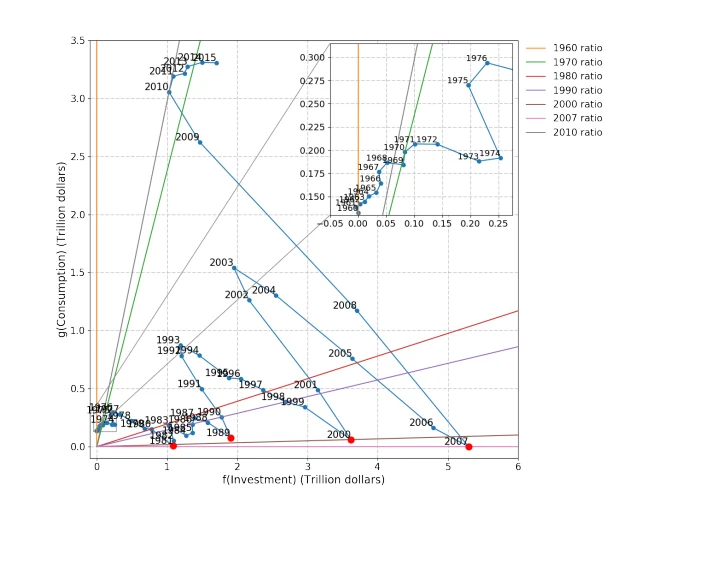
\includegraphics[width=17cm]{images/Libro-img041.png}
    \caption{Rapporto tra investimenti e consumi, per anno, in miliardi di dollari. Credits: Complex Systems Institute/Yaneer Bar-Yam}
  \end{minipage}
\end{figure} 

Dall'insediamento di Reagan nel 1980, i consumatori hanno accumulato 13.000 miliardi di dollari di debito, mentre gli
investitori hanno accumulato miliardi di
capitali\endnote{\protect\url{https://www.bloomberg.com/news/articles/2017-06-06/trump-s-america-is-facing-a-13-trillion-consumer-debt-hangover}
}.

\bigskip

Bar-Yam e i suoi colleghi hanno analizzato i dati storici e hanno creato dei modelli i quali dimostrato che l'approccio
dell'amministrazione Trump volta alla crescita economica riducendo la spesa pubblica e abbassando le aliquote fiscali
per i ricchi, è errato.

Una soluzione efficace implicherebbe una serie di sovvenzioni, tra cui, introdurre il salario minimo, alleggerire il
debito, o eliminarlo per pagarsi gli studi. Tutte manovre che consentano ai meno abbienti di poter accedere a beni e
servizi per far girare l'economia, cosa che attualmente sono scoraggiati a fare causa gli enormi
debiti che sono costretti a sostenere. 

Senza questi incentivi, è improbabile che il capitale venga investito e che l'economia
cresca\endnote{\protect\url{https://www.vice.com/it/article/xwge9a/la-matematica-consiglia-non-tagliate-le-tasse-redistribuite-la-ricchezza}
}.

La politica economia del gocciolamento dall'epoca di Reagan ipotizza che se i più ricchi spendono
soldi per cose che non siano tasse, ma presumibilmente orientate al potenziamento della propria azienda, la situazione
economica dei lavoratori migliorerà di conseguenza. Ma anni di dati ci dimostrano non essere
così\endnote{\protect\url{https://www.ted.com/talks/jonathan\_smith\_do\_tax\_cuts\_stimulate\_the\_economy} \ }.


\bigskip

Il liberismo, ovvero l'idea che il mercato deve essere libero da interventi dello stato, sembra una
scelta corretta, ma i grandi monopolisti e i corrotti non faranno mai gli interessi della maggioranza. Lo stato non
interviene per essere un limite all'economia, ma per dare istruzione ai poveri, assistenza
sanitaria, protegge l'ambiente, gestire la crisi economiche, ecc… 


\bigskip

Nel grande come nel piccolo abbiamo fondato la nostra economia sul debito anziché sul credito. E permeato molto nel
tessuto sociale indebitarsi per fare acquisti. A volte è necessario, comprare una casa senza un mutuo è praticamente
impossibile. Se ti si rompe il frigorifero, la caldaia o la macchina, beni necessari, è normale aprire un prestito. Il
debito è necessario a volte, ma dovrebbe essere evitato il più possibile. I soldi non danno la felicità, ma avere una
sicurezza economica fa vivere con qualche pensiero in meno. Per riuscire a scappare dalla paura di fronteggiare spese
necessarie alla propria sopravvivenza e non trovarsi senza soldi o si guadagna bene o si risparmia bene. Entrambi
obiettivi percorribili, ma è probabile che la maggior parte di noi si troverà a gestire uno stipendio che va dal medio
basso al medio alto, lasciando come unica scelta per la stabilità economica il risparmio. Anche qua ritorna il discorso
dell'accettazione: probabilmente non saremo mai ricchi. Forse è duro da accettare ma è così. Ma va
bene lo stesso, si può vivere benissimo e felici anche da benestanti. Il problema del debito, sono gli interessi. Gli
interessi sono soldi sprecati, non ti arricchiscono, non ti offrono beni o servizi e non sono pochi! A conti fatti, per
certe spese, si arriva a spendere circa il doppio! Se ci troviamo nella situazione di dover aprire un mutuo, significa
che in quel momento non abbiamo sufficienti risparmi da parte. Il problema di non avere risparmi è che non possiamo
prevedere il futuro. Potrebbe rompersi la caldaia, una tubatura, scoppiare una pandemia o fallire
l'azienda per cui lavoriamo e perdere il lavoro. Siamo portati a pensare che non succederà mai a
noi, ma queste cose succedono! Queste situazioni posso portarti da una vita spensierata fatta di ristoranti, aperitivi,
discoteche, viaggi ecc… Al dramma più nero. Bisognerebbe riuscire a fare scelte lungimiranti oggi per ottenere una
stabilità. Non serve vivere nella miseria. Tante scelte economiche non cambiano lo stile di vita.

\begin{enumerate}
\item Evitare i debiti il più possibile: Se devi comprare un televisore è meglio risparmiare. Anche se passerai un
periodo senza. Non aprire un mutuo. Se non puoi fare a meno di chiedere un prestito, cerca di pagare l'anticipo più
alto possibile, per diminuire numero di rate e relativi interessi.
\item Crea un fondo di emergenza: Almeno 1.000 euro, ma meglio se di più, che non può essere toccato per nessuna
ragione, se non per le emergenze.
\end{enumerate}

\bigskip

Ma come creare un fondo d'emergenza? Una regola molto efficace è chiamata 50/20/30. Cosa significa?
Significa che il 50\% delle nostre entrate deve essere destinato alle spese essenziali, affitti, bollette, trasporto e
cibo. Tutte quelle spese che più o meno tutti ci troviamo ad affrontare mensilmente è che non possiamo evitare. Il 30\%
sono le spese “extra” come cinema, ristoranti, uscite con gli amici ecc… Infine il 20\% è la cifra da risparmiare.


\bigskip

50\% spese essenziali

Le vostre spese essenziali superano il 50\% del vostro reddito? Analizziamolo in maniera scientifica. Questo potrebbe
essere un po' impegnativo e scoraggiare la maggioranza ma è fondamentale. Bisogna segnarsi tutte
le spese e catalogarle come spesa, ristorante, cura personale, salute, trasporti ecc… Potete utilizzare un taccuino, un
foglio elettronico, un app. Ad oggi tutte le app della banca fanno questa divisione al posto nostro, offrendoci anche
altre numerose statistiche. Se però prelevate denaro, la banca non potrà sapere in quale categoria è stato impiegato e,
dovrete quindi farlo voi manualmente. Questo è l'unico modo per poter analizzare dove spendiamo di
più e pensare ad un modo per ridurlo. Possiamo cambiare operatore di luce e gas, consumare meno, abbassare la
temperatura di casa da 22° a 18° e mettersi un maglione in più, che aiuta l'ambiente e le nostre
finanze. Trovare un affitto più economico. Ma gli ambiti dove forse si risparmia di più sono trasporti e alimentari.
Provate a fare il conto di quanto risparmiereste all'anno se sostituiste i cibi pronti con gli
ingredienti per preparare lo stesso piatto. \ Potete scegliere di andare ad un discount. Fate il conto di quanto vi
costa mangiare in pausa pranzo al lavoro rispetto a portarvelo da casa. Questo vi permetterà di risparmiare oltre 500
euro. O ancora, fate lo stesso conto se pensate di prendere la macchina per raggiungere la stazione dei treni, più
l'abbonamento rispetto a raggiungere il posto di lavoro in auto. Esistono anche biciclette e
monopattini pieghevoli per coprire anche l'ultimo pezzo di strada, dalla stazione
all'ufficio. Inoltre sul treno/pullman potete leggere, guardare un film, lavorare, dormire.
Diversi studi dimostrano che i soldi non danno la felicità, a meno che li usiate per avere più tempo. Sembrano
sciocchezze ma parliamo di centinaia di euro all'anno che potete risparmiare facilmente, senza
cambiare il vostro tenore di vita, anzi, migliorandolo. Secondo alcuni studi i Masai dell'Africa
orientale abbiano un indice di soddisfazione della vita simile a quello dei 400 americani più ricchi nella lista di
Forbes.


\bigskip

30\% spese personali

Sempre guardando il nostro taccuino, app o foglio elettronico, possiamo analizzare dove possiamo ridurre le spese. Un
modo semplice è evitare la lotteria, schedine, gratta e vinci. Le probabilità di vincita sono bassissime, difficile
quantificare quanto siano basse. C'è una probabilità più alta di vedere una tigre siberiana in
centro a Milano che vincere alla lotteria. Un latro esperimento da fare è il conto annuo di sigarette, alcolici, bar,
caffè alle macchinette ecc… anche qua si possono risparmiare diverse centinaia di euro. Internet e le app possono
permetterci di viaggiare, comprare beni e servizi, al miglior prezzo. Se anche risparmiando al massimo, non riusciamo a
far stare le spese essenziali nel 50\% dello stipendio, dovremmo andare a ridurre questo 30\% di spese e, cercare di
ottenere un entrata maggiore, con un aumento o cambiando impiego, senza lasciare il lavoro attuale. Solo quando si
riesce a trovare un nuovo impiego si può abbandonare quello vecchio.


\bigskip

20\% risparmio

Il modo più semplice per risparmiare denaro è assicurarti che tu non abbia la possibilità di spenderlo. Potete
addebitare automaticamente una parte del vostro stipendio direttamente in un libretto di risparmio o in un fondo
pensionistico.

Come abbiamo visto, individuare le spese maggiori ci indica dove intervenire per risparmiare. Per questo motivo è
indicato dedicare più tempo nelle macro spese della vita, come casa e auto. Case equiparabili per metratura, servizi,
efficienza energetica ecc… possono avere prezzi molto differenti tra loro. Quindi a parità di casa ci troveremo con
diverse migliaia di euro in meno da spendere. Stesso discorso per l'auto. In Italia per cambiare
auto si spende mediamente 21.500
euro\endnote{\protect\url{https://www.sicurauto.it/news/attualita-e-curiosita/auto-nuova-gli-italiani-hanno-speso-in-media-21-mila-euro-nel-2019/}
}. Possiamo trovare utilitarie a chilometro zero spendendo circa la metà, consentendo di risparmiare 10.000 euro facili
facili che possiamo impiegare per altro. Un'utilitaria da cinque posti permette di muovere
agevolmente una famiglia media, di fare la spesa e hanno la stessa vita di una macchina più costosa. In Italia la vita
media di una macchina è di circa 10 anni. Quindi in una vita potremmo possedere circa cinque o sei macchine, significa
che abbiamo un ambito dove possiamo avere un risparmio potenziale di 60.000 euro. Questo è un discorso che si presta
soprattutto nei primi anni di vita, magari tra i 20 e i 40 anni. Ma se uno guadagna bene, ha risparmiato bene, ci tiene
ad avere una certa macchina, non ha senso che se la privi. La vita è una questione di priorità. Uno può spendere anche
40.000 euro per una macchina a 20 anni, perché gli piace e, aprire un mutuo. Consapevole però che non è necessario, che
con gli interessi andrà a pagarla molto di più e che se dovesse perdere il lavoro, oltre a non poterla più pagare
potrebbe far fatica a mangiare. Eliminare \ il superfluo è il modo più semplice per risparmiare, aperitivo, colazione
al bar ecc… Sono pochi soldi, ma tutti i giorni fanno un grosso volume. O come per l'auto, un
grosso volume per una sola volta. Si tratta di priorità. Se si ipotizza che in un futuro le cose potrebbero essere
diverse, rinunciare ad una macchina costosa a fronte dell'ansia di non arrivare a fine mese, per
tutti i mesi, non penso ci sia paragone. Se dovessi perdere il lavoro per quanto riusciresti a sopravvivere? Nemmeno un
mese? Meglio prendere un utilitaria. Un anno? Due anni? In questo tempo puoi trovarti un nuovo lavoro per cui si può
valutare.

Meglio una macchina nuova ogni 10 anni o una macchina usata ogni anno? Da buon programmatore mi sono costruito un
programma che otteneva informazioni da siti di auto usate. Il programma in base agli anni e ai chilometri fatti dalla
macchina faceva una stima di quanta vita potesse ancora avere in relazione al suo costo. Il risultato è stato che in
una vita, si va a spendere di più comprando economiche auto usate rispetto a comprare un auto nuova. Se il paragone lo
facciamo con auto a chilometro zero, diventa ancora più vantaggioso comprare un auto nuova. Questo ragionamento è fatto
considerando l'acquisto di un auto senza prestito. Se dovete fare un prestito la risposta è:
dipende. Dipende dagli interessi. L'ideale è un auto nuova a chilometro zero \ o a tasso zero.
Inoltre un utilitaria ha dei costi minori in termini di bollo, assicurazione e benzina.


\bigskip

Alcuni trucchi:

\begin{itemize}
\item Una volta deciso il budget da spendere per le varie categorie. Se fatichi a rispettare queste soglie puoi a inizio
del mese, preparare delle buste, una per ogni categoria, con all'interno il relativo budget. Ogni
volta che si deve affrontare una spesa si possono utilizzare le buste, ma una volta che è finito, è finito, non si può
prelevarne altro.
\item Metodo delle 24 ore: Ogni volta che si ha un desiderio, impulsivo, di comprare qualcosa, darsi almeno 24 ore di
tempo prima di comprarlo davvero. A volte il desiderio svanisce da solo.
\item Spendi per risparmiare. Ogni volta che fai una spesa “extra” come un gelato, poni lo stesso ammontare sul tuo
conto di risparmio.
\end{itemize}

\bigskip

\clearpage\section{Curiosità}
Siamo quasi giunti al termine, mi auguro di non avervi fatto annoiare e spero davvero di aver scritto qualcosa che via
abbia incuriosito, interessato, che non sapevate o che possa tornarvi utile.

Vorrei concludere raccogliendo delle curiosità che probabilmente non vi torneranno utile ma che a me hanno affascinato e
incuriosito.

\subsection{App per imparare}
Inizio questo capitolo con le app che più utilizzo per informarmi.

\begin{itemize}
\item Feedly: Ci sono tanti siti che pubblicano news su cui vorrei rimanere aggiornato, ma andare periodicamente su
ognuno di questi siti per vedere gli aggiornamenti può diventare un lavoro impegnativo. Feedly ci viene in contro in
quanto ci permette di aggiungere in un unico posto tutte le nostre fonte di informazioni e vedere ogni nuovo articolo
che viene pubblicato. Tra i miei siti preferiti troviamo: Focus, National Geographic, TedVice, Wired. Oltre ai siti si
possono aggiungere podcast, come Daily cogito e Psinel o canali Youtube come quello di Just Mick, Luca Mazzucchelli e
Wesa channell.
\item Google Play Books: Per quanto riguarda la lettura di libri apprezzo Google Play Books, perché oltre ad essere
forse il più grosso store, l'app per smartphone ha anche la funzione di sintesi vocale. Questa
funzione permette di farsi leggere il libro da una voce artificiale. Questa lettura, essendo fatta da un software e non
da una persona in carne ed ossa, non risulta certamente espressiva, ma nemmeno così robotica come ci si potrebbe
immaginare. Dopo poco ci si abitua e l'esperienza risulta più che fruibile. Ho iniziato ad
apprezzare questa funzione durante i miei viaggi in macchina di circa un ora per raggiungere il luogo di lavoro.
Sentivo che quel tempo poteva essere impiegato in modo migliore e così ho introdotto la lettura.
\item Ereader Prestigio: Se abbiamo dei documenti in Pdf, al momento della stesura di queste righe, Google Play Books
non permette la sintesi vocale. Per questo possiamo utilizzare eReader. Entrambe le applicazioni consentono di
impostare la sintesi vocale a velocità diverse. Possiamo impostarla a 1,25x, 1.5x, 1,75x o 2x, con
quest'ultima opzione significa che il lettore parlerà due volte più veloce del normale.
\protect\url{https://play.google.com/store/apps/details?id=com.prestigio.ereader} 
\item Vflat: Non sempre però i libri che vogliamo esistono in formato cartaceo. Se come me, apprezzate di più il libro
digitale invece che cartaceo potete utilizzare vFlat, un app che consente, utilizzando la fotocamera del cellulare, di
scannerizzare un libro. L'app è veramente ben fatta! Un intelligenza artificiale rimuoverà le
vostre dita, mentre tengono il libro aperto, dalla foto. Non servirà schiacciare un pulsante ogni volta che girate la
pagina, l'app capirà automaticamente che avete girato la pagina e farà la foto, rendendo molto
veloce la scansione. In 10 minuti è possibile fare 200 o 300 pagine senza sforzo. Questo anche perché possiamo
fotografare due pagine contemporaneamente e l'app dividerà l'immagine nelle
due pagine. Inoltre, l'app correggerà la curvatura delle pagine e bilanciando il bianco, facendola
sembrare una vera scansione più che una fotografia. L'app ha anche una funzione di Ocr, che
permette di estrapolare testo dalle immagini in modo da poter essere letta anche da eReader.
L'ideale è riuscire a utilizzare un treppiede o qualcosa che ci possa consentire di lasciarci le
mani libere in modo da poter sfogliare le pagine. \protect\url{https://play.google.com/store/search?q=vflat} 
\item Google Podcast e Youtube: Fin ora abbiamo visto come fruire di contenuti testuali, ma da casa Google troviamo
quelle che secondo me sono le app più ricche di contenuti per quanto riguardano podcast e video.
\end{itemize}
\subsection{Sokushinbutsu}

\begin{wrapfigure}{i}{9cm}
  \centering
  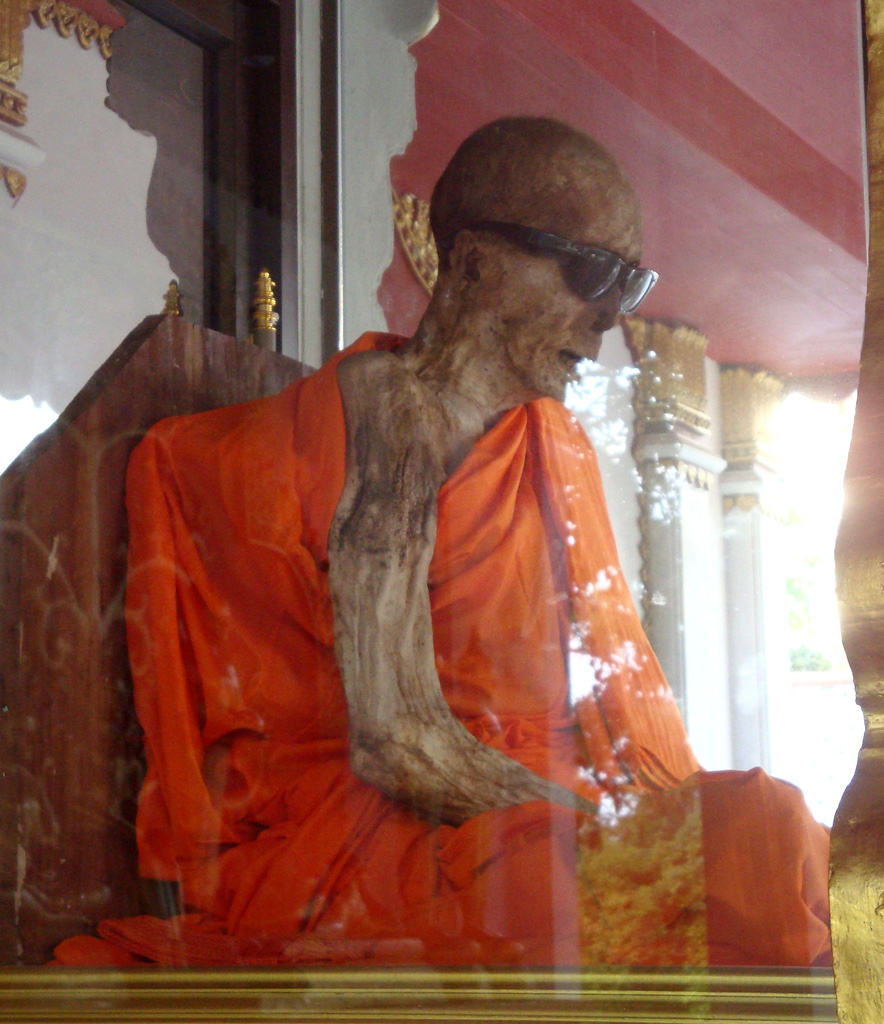
\includegraphics[width=0.95\linewidth]{images/Libro-img042.jpg}
  \begin{minipage}{\linewidth}
    \caption{Credits: Di Per Meistrup, CC BY-SA 3.0, \protect\url{https://commons.wikimedia.org/w/index.php?curid=19168593}}
  \end{minipage}
\end{wrapfigure}

Questa cosa mi ha letteralmente scioccato, si tratta di un rituale religioso buddhista, praticato dai monaci giapponesi
i quali, attraverso un lungo processo che terminava con la morte riuscivano ad automummificarsi. 

Questo processo, che si svolge da vivi, si divide in tre fasi, ognuna della durata di mille giorni dove progressivamente
ci si priva del cibo e si incrementa la meditazione e l'esercizio fisico.

Nella prima fase, il monaco si reca in una valle chiamata Senninzawa ({\textquotedbl}Palude degli
immortali{\textquotedbl}), dove medita, fa esercizio fisico e, mangia solo noci e semi, in modo da far perdere massa
grassa all'organismo.

Successivamente nella seconda fase, il monaco che nei precedenti mille giorni avrà già eliminato quasi completamente i
grassi corporei, inizierà una dieta ancora più deprivante, nutrendosi soltanto di piccole quantità di corteccia, aghi e
radici di conifere, sempre mantenendo il corpo e la mente in attività, attraverso esercizio fisico e meditazione. Verso
la fine della seconda fase, il monaco inizierà ad assumere un tè tossico a base di urushi (Toxicodendron vernicifluum),
una pianta velenosa la cui linfa veniva generalmente utilizzata per laccare le ceramiche provocando all'organismo forte
nausea, sudorazione e diuresi, così da perdere altri liquidi corporei. Inoltre diventeranno tossici anche i tessuti
interni, così una volta cadavere sarà repellente per le larve e gli altri insetti che altrimenti se ne ciberebbero.

Nell'ultima fase il monaco entrerà in una cripta in pietra, grande a malapena per contenere il suo
corpo nella posizione del loto. Dopodiché la cripta viene sigillata, il monaco è senza acqua e cibo e solo una cannula
di bambù permetterà il ricambio d'aria. Il monaco dentro questo loculo che sarà la sua tomba fa risuonare di tanto in
tanto una campanella. Quando non avrà più le energie per suonare la campanella i monaci
all'esterno rimuoveranno il bambù e sigilleranno completamente la cripta. Il monaco ancora vivo,
grazie al suo respiro rimuoverà il poco ossigeno presente all'interno della cripta, riducendo così
ulteriormente la possibilità che possano svilupparsi forme di vita che potrebbero far marcire la carne, in questo modo
però, morirà anche lui stesso agonizzante per asfissia. La cripta rimarrà chiusa per altri mille giorni e, quando verrà
riaperta se il corpo sarà correttamente mummificato, avrà raggiunto la condizione di Buddha e divenà oggetto della più
profonda venerazione, se invece il corpo si manifesta tracce di putrefazione la cripta sarà nuovamente sigillata e il
monaco, anche se non potrà essere considerato un Buddha, sarà comunque rispettato e ammirato per il durissimo percorso
di privazioni volontariamente intrapreso. 

Se farete un viaggio in Giappone potete visitare i tempi dove sono esposti questi corpi. Anche se la pratica fu
intrapresa, nel corso dei secoli, da diverse centinaia di monaci, i corpi di solo 24 di questi sono giunti fino ai
giorni nostri. Dal 1877 questa pratica è diventata illegale, anche se l'ultimo monaco che l'ha
portata a termine con successo è deceduto nel 1903\endnote{\protect\url{https://it.wikipedia.org/wiki/Sokushinbutsu} }.


\bigskip

\subsection{Tribù incontattate}

\begin{wrapfigure}{i}{9cm}
  \centering
  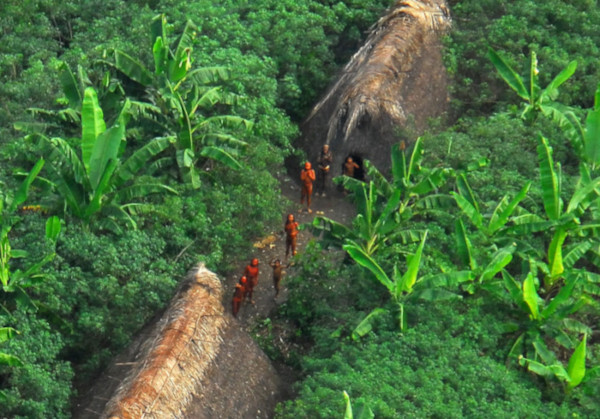
\includegraphics[width=0.95\linewidth]{images/Libro-img043.jpg}
  \begin{minipage}{\linewidth}
    \caption{Credits: Di Agência de Notícias do Acre: Gleilson Miranda / Governo do Acre -
\protect\url{https://www.flickr.com/photos/fotosdoacre/3793141477/,} CC BY 2.0,
\protect\url{https://commons.wikimedia.org/w/index.php?curid=18968640} }
  \end{minipage}
\end{wrapfigure}

Sono quei popoli indigeni che non hanno contatti con la civiltà moderna, secondo Survival International, le tribù
incontattate nel mondo sarebbero almeno 100. Nonostante il grado di conoscenza che abbiamo del nostro pianeta tutti gli
anni vengono scoperte nuove forme di vita vegetali e animali, ma ancora più incredibile è che ogni tanto vengono
scoperti nuovi gruppi di esseri umani. Nel 2009 in Brasile, dove si stima essere presente la maggior parte di questi
popoli, sono stati avvistati da un elicottero un nuovo gruppo di indigeni (immagine qui di fianco). 

La difficoltà di avere contatti con queste popolazioni è che spesso, quando avvengono contatti con noi occidentali
facciamo contrarre loro malattie e forme di influenza che non conoscono e di cui non hanno anticorpi e che possono
portare alla decimazione di queste comunità.

\begin{wrapfigure}{i}{9cm}
  \centering
  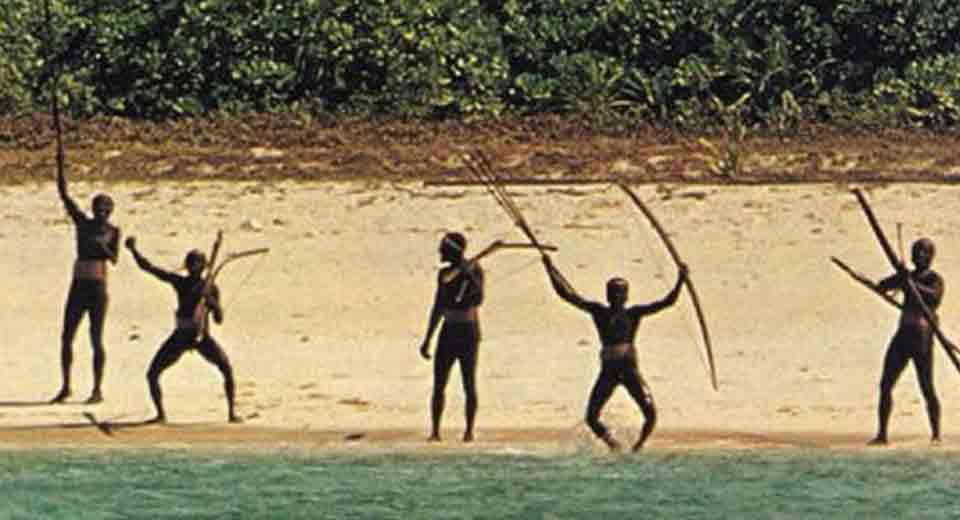
\includegraphics[width=0.95\linewidth]{images/Libro-img044.jpg}
  \begin{minipage}{\linewidth}
    \caption{Credits: Estratto di un filmato sulla tribù di north
sentinel che reagisce con arco e frecce agli estranei, Credit: Survival International}
  \end{minipage}
\end{wrapfigure}

Tra queste, la più isolata in assoluto è quella dell'Isola di North Sentinel nel golfo del Bengala.
Questa popolazione non conosce il remo per poter allontanarsi dall'isola e
l'India ha proibito di avvicinarsi in quanto, i numerosi tentativi di stabilire un contatto con
queste popolazioni si sono conclusi in modo violento da parte degli indigeni. Ci sono alcuni video risalenti agli anni
70 che potete trovare su internet del tentativo di avvicinarsi a questa comunità le quali hanno risposto scagliando
numerose frecce. Questa comunità è stata dichiarata da Survival International, la società più vulnerabile del pianeta,
in quanto una piccola epidemia potrebbe spazzare via i 50 abitanti (circa) di questo luogo.

\bigskip

\subsection{Intelligenza artificiale}
Sentiamo spesso parlare di intelligenza artificiale, un sacco di dispositivi che abbiamo a casa la utilizzano, per
esempio l'algoritmo che mette un quadratino attorno alle facce mentre facciamo una fotografia con
la nostra macchina fotografica o smartphone. La possibilità di scrivere un messaggio senza digitare le lettere sulla
tastiera, ma semplicemente parlando. Fino ad arrivare a cose più futuristiche, ma che in alcuni stati possiamo già
trovare, come le auto a guida autonoma. Le applicazione sono attualmente tantissime. Questo è un campo dove
c'è ancora una forte ricerca con quotidiane scoperte, che danno questa tecnologia un fortissimo
potenziale, che vedremo realmente esprimersi nei prossimi anni. Queste tecnologie sembra che funzionino come per magia
e, non conoscendole, possono farci anche paura. La filmografia è piena di esempi di robot che prendono il controllo
diventando i padroni dell'umanità. Vi voglio tranquillizzare su vari punti. Questa paura nasce in
primo luogo per un errore, che ci porta a proiettare ambizioni del tutto umane anche all'esterno
di altre specie, viventi e non. Le macchine infatti non hanno alcuna ambizione a diventare la specie più potente della
terra e, avere il predominio del mondo. Questo è un desiderio tipicamente umano. Secondo punto, come visto nel film “Io
robot” con Will Smith, esistono delle regole su cui si basa la robotica che sono state scritte da Isaac Asimov:

\begin{enumerate}
\item Un robot non può recar danno a un essere umano né può permettere che, a causa del suo mancato intervento, un
essere umano riceva danno.
\item Un robot deve obbedire agli ordini impartiti dagli esseri umani, purché tali ordini non vadano in contrasto alla
Prima Legge.
\item Un robot deve proteggere la propria esistenza, purché la salvaguardia di essa non contrasti con la Prima o con la
Seconda Legge."
\end{enumerate}
Tantissima della tecnologia che abbiamo oggi è stata inventata dalla letteratura e dalla filmografia e poi realizzata
dall'ingegneria. Ci sono tantissimi esempi tra gli scrittori come Isaac Asimov, Philip K. Dick e
nella filmografia come ad esempio la serie Star Trek che ha concepito il telefonino, porte automatiche, il traduttore,
videoconferenze, GPS, tablet e tanto altro. Ancora più incredibile è pensare che già attorno agli anni 50 alcuni
scienziati avevano già teorizzato tecniche che ancora oggi usiamo e, che sono state alla base della ricerca. Purtroppo
questi pionieri dell'intelligenza artificiale, non hanno potuto mettere in pratica le loro teorie,
siccome la potenza di calcolo dei computer non era nemmeno lontanamente paragonabile a quella attuale. Tra questi
scienziati troviamo Warren Sturgis McCulloch (neurofisiologo), Walter Pitts (matematico), \ Frank Rosenblatt (psicologo
e computer scientist americano), Alan Turing (matematico) e tanti altri.

Infine, l'intelligenza artificiale (IA) non dovrebbe spaventarci perché non ha consapevolezza o non
ancora. Infatti le IA anche se sembrano umane riuscendo ad ascoltare, parlare, imparare, migliorandosi e prendendo
decisioni, seppur molto flessibili, il loro comportamento è stato deciso da programmatori.

Il compito degli informatici, riducendo al massimo è: risolvere problemi. E l'informatica è uno
degli strumenti per risolvere problemi. L'informatica stessa utilizza diverse strategie che si
ramificano e sottoramificano in diversi metodi con pro e contro per la tipologia di problema. Solitamente un programma
informatico è un insieme di istruzioni semplici, eseguite sequenzialmente, che prende il nome di algoritmo. Per creare
questo programma informatico devono essere chiare nella mente del programmatore le istruzioni, i passaggi, le formule e
tutto quello che l'algoritmo dovrà eseguire. È come un libretto delle istruzioni con tutti i
passaggi da svolgere. Alcuni problemi però sono molto complessi. Per tanti motivi, ci sono troppe variabili, troppi
casi particolari e, ad oggi non sono ancora state create le istruzioni per risolvere questo problema. 

Immaginate un programma per riconoscere la foto di un gatto. Senza IA, con uno sforzo considerevole si potrebbe dare le
istruzioni a un programma per individuare le orecchie a punta, i baffi, gli occhi grandi ecc… Ma con regole così
rigide, se gli sottoponessimo la foto di una tigre, non saprebbe trovare le differenze con un gatto, per cui serve una
capacità di astrazione maggiore. Se pensiamo di costruire un programma per la guida autonoma
dell'auto, nessuna persona al mondo, nemmeno la più intelligente, può gestire
quest'infinito numero di variabili. Il che è strano, perché in tanti sanno guidare una macchina,
lo facciamo tutti i giorni, non sapremmo spiegarlo a livello semplice, senza astrazione. Immaginate di dover spiegare
un riflesso, come valutare pericolo, anche fare solo una lista di tutti i potenziali pericoli, ti può attraversare uno
scoiattolo, trovare una parata, un carro funebre, un camion che perde parte di carico, sono praticamente infinite e, in
infiniti modi si può reagire ad ogni stimolo. E questa è solo una piccola parte del problema. 

Per un essere umano questi compiti sono piuttosto facili. Ma il computer, che siamo portati a pensare essere molto
intelligente, in realtà non lo è. Un computer non sa fare cose complicate ma sa unire tante cose semplici per farne una
complessa e, lo sa fare velocemente. L'essere umano è lento, ma può creare, ragionare e astrarre,
a differenza di una macchina che sa solo eseguire. Anche quando crea musica o arte, grazie all'IA
sta comunque eseguendo un compito con possibilità di variare, ma solo entro certi schemi, le cui possibilità possono
comunque essere infinite.

L'informatica “classica”, quindi, per fornire un risultato (output) all'utente
che utilizza un programma o un app, identifica le informazioni che l'utilizzatore dovrà inserire
(input), come ad esempio, nel caso di una mail, sono destinatario, oggetto e corpo del messaggio. A questo punto il
programmatore dovrà creare tutti i comandi (algoritmo) per recapitare il messaggio al relativo destinatario. Quindi si
ha un input, il programma lo elabora e si ha un output, ad esempio la spedizione del messaggio. Con
l'IA si parte anche qui da un input e da un output, ma per via della complessità non si può creare
un algoritmo. Così si lascia che sia la macchina a comprendere la relazione tra input e output, di come un certo input
genera un certo output, creando autonomamente l'algoritmo.


\bigskip

l'IA consente di risolvere tre principali problemi: 

\begin{itemize}
\item Classificazione: Abbiamo un dato e vogliamo dargli un nome, un etichetta (label). Ad esempio, facciamo una foto a
un fiore e vogliamo sapere di che specie si tratta. Il numero di etichette che il programma può fornirci è limitato.
\item Regressione: Abbiamo serie di valori e vogliamo trovare il risultato. Ad esempio, una casa, di x metri quadri, con
x camere, nella x zona, con x servizi ecc… costerà y euro. La regressione ci può fornire potenzialmente infiniti
risultati, un numero qualsiasi con la virgola compreso tra meno infinito e più infinito.
\item Clustering: In questo caso vogliamo fare una classificazione, di cui però non conosciamo le etichette. Per
esempio, quali sono stati i trend di quest'anno?
\end{itemize}

\bigskip

Per funzionare un IA ha bisogno di due fasi, l'apprendimento e la predizione.
L'intelligenza artificiale copia il funzionamento umano. Esattamente come noi umani, impariamo per
esempi.

Facciamo un esempio di classificazione.

\begin{wrapfigure}{i}{9cm}
  \centering
  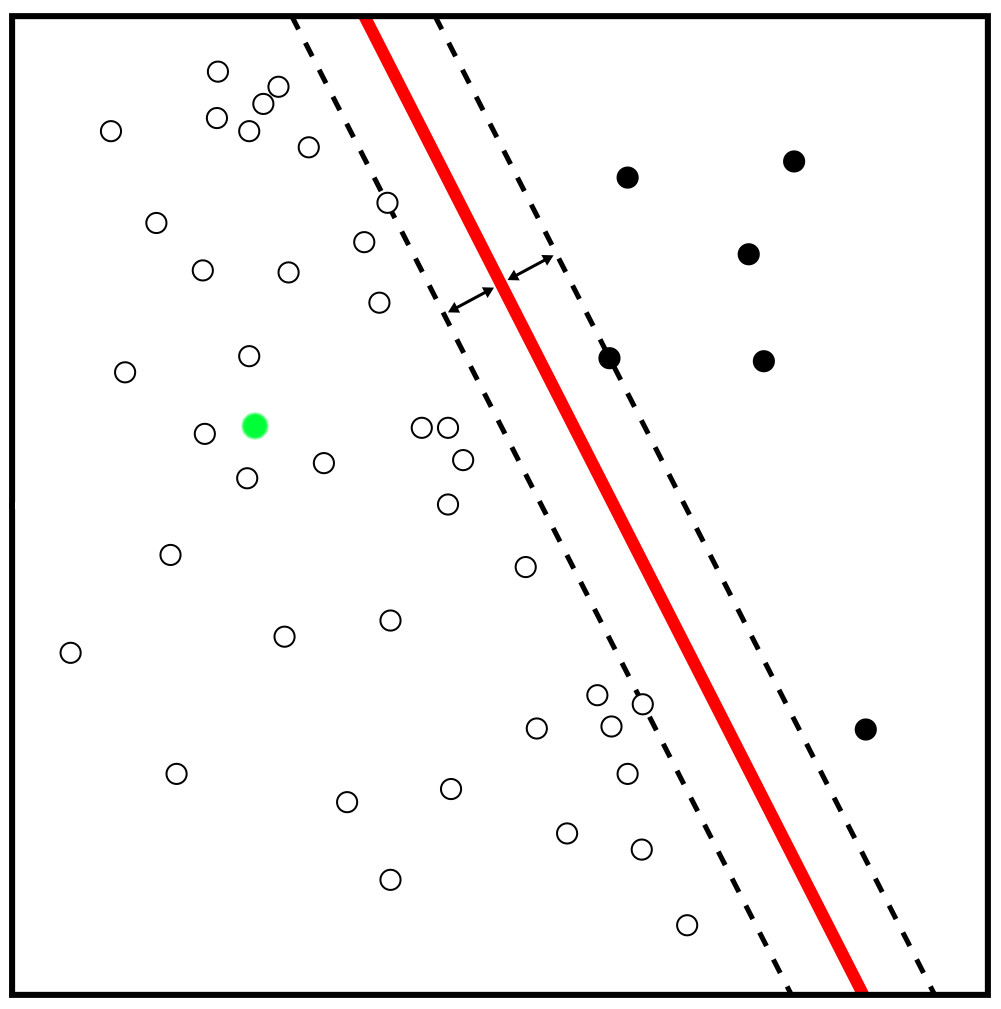
\includegraphics[width=0.95\linewidth]{images/Libro-img045.jpg}
  \begin{minipage}{\linewidth}
    \caption{By Alisneaky, svg version by User:Zirguezi - Own work,
CC BY-SA 4.0, \protect\url{https://commons.wikimedia.org/w/index.php?curid=47868867} }
  \end{minipage}
\end{wrapfigure}

Se vogliamo creare un IA che sappia riconoscere l'esatta specie del fiore Iris, dobbiamo prima di
tutto definire qual'è la discriminante, quali sono le caratteristiche che fanno la differenza tra
una specie e l'altra? Ad esempio la larghezza e la lunghezza dei petali. Nella prima fase, di
apprendimento, va fatta la raccolta dei dati, tantissimi dati. Quindi ci mettiamo a misurare larghezza e altezza di
tantissimi Iris. Abbiamo preso solamente due specie in questo esempio, quelle indicate dal pallino nero e quelle
indicate dal pallino bianco. Se un giorno, andassimo a fare un escursione, con in mano questo grafico e, incontrassimo
un Iris, con una semplice misurazione, rappresentata dal pallino verde, a colpo d'occhio possiamo
subito capire che fa parte della stessa specie dei pallini bianchi, questa è la predizione. Un computer però non
possiede la funzione “colpo d'occhio”. Perché per un computer non esistono forme, non esistono
colori, linee ecc… esiste solo 0 e 1. Questo grafico si può tradurre in qualcosa tipo
010100011101110100011011000011100… in questo caso sarebbe impossibile per noi avere
l'interpretazione che lo stesso grafico ci mostra così chiaramente. Quindi nella fase di
apprendimento verranno dati in pasto all'IA tutte le misurazioni e, ad ogni misurazione che gli
viene fornita, con dei metodi statistici, tra cui la classificazione bayesiana (basata sul teorema di Thomas Bayes
(1702-1761)) crea quella linea rossa. Più esempi abbiamo, più quella linea saprà separare correttamente le due classi,
le due tipologie di Iris. Una volta che abbiamo questa retta, possiamo anche buttare via tutte le misurazioni, il
modello a questo punto può essere indipendente. Se ci trovassimo di fronte a un fiore, misurando i petali e segnandoli
sul piano cartesiano del grafico, ci basterà vedere se si trova a destra o a sinistra della linea per fare la nostra
predizione. Le strategie che vedremo per la risoluzione dei tre problemi fondamentali dell'IA sono
solo un esempio, non sono le uniche. Di seguito una rappresentazione del vasto mondo dei classificatori.

\begin{figure}[H]
  \begin{minipage}{17cm}
    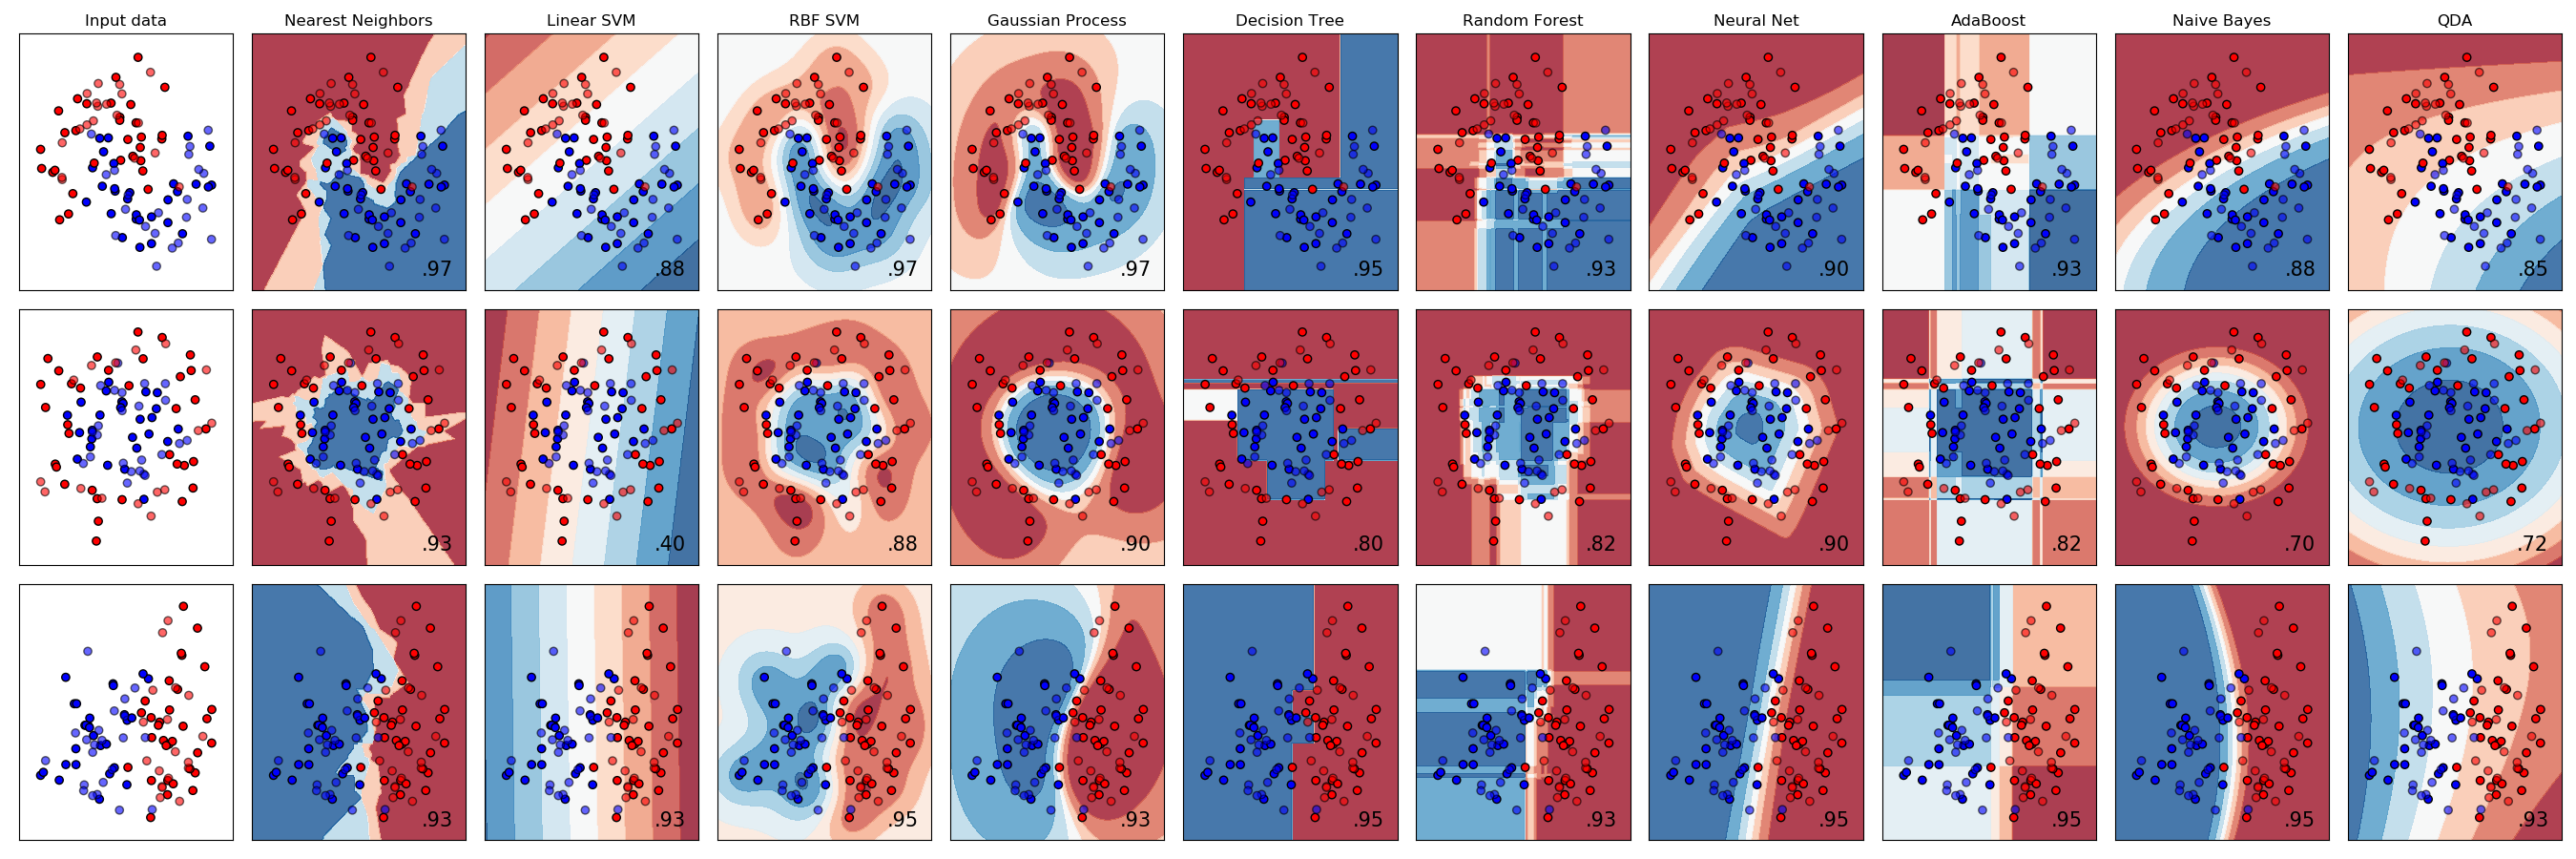
\includegraphics[width=17cm]{images/Libro-img046.png}
    \caption{Credits: Scikit Learn \protect\url{https://scikit-learn.org/stable/auto\_examples/classification/plot\_classifier\_comparison.html} }
  \end{minipage}
\end{figure}

\begin{wrapfigure}{i}{9cm}
  \centering
  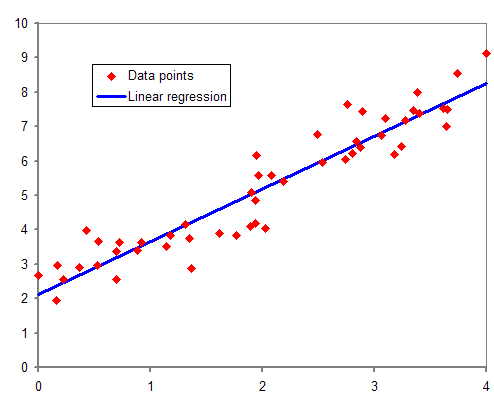
\includegraphics[width=0.95\linewidth]{images/Libro-img047.png}
  \begin{minipage}{\linewidth}
    \caption{Di Amatulic di Wikipedia in inglese (same as
Anachronist on Wikimedia) - Trasferito da en.wikipedia su Commons. Transfer was stated to be made by User:anachronist.,
Pubblico dominio, \protect\url{https://commons.wikimedia.org/w/index.php?curid=3337769} }
  \end{minipage}
\end{wrapfigure}

Se ci trovassimo ad affrontare un problema di regressione, l'unica cosa che cambia è il metodo
statistico utilizzato. Avremmo sempre una fase di apprendimento dove forniamo all'IA le nostre
misurazioni, rappresentata dai rombi rossi e il programma creerebbe la linea blu, utilizzando ad esempio la formula
statistica della regressione lineare. A questo punto, l'intelligenza può predirre il valore di y
nel caso in cui la x fosse 7, quindi un dato esterno al nostro grafico. Con questo metodo possiamo fare anche
previsioni su eventi futuri.

\begin{wrapfigure}{i}{9cm}
  \centering
  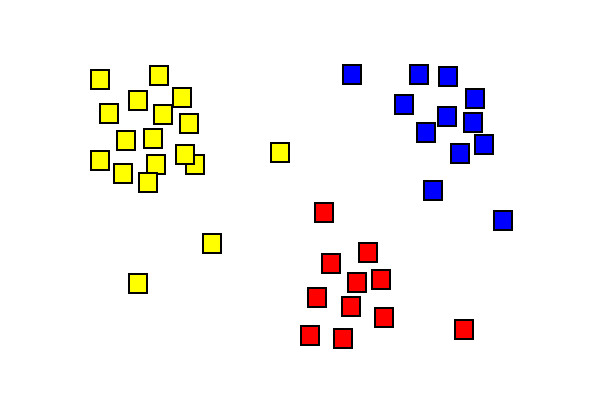
\includegraphics[width=0.95\linewidth]{images/Libro-img048.jpg}
  \begin{minipage}{\linewidth}
    \caption{By Cluster-2.gif: hellispderivative work: Wgabrie
(talk) - Cluster-2.gif, Public Domain, \protect\url{https://commons.wikimedia.org/w/index.php?curid=9442336} }
  \end{minipage}
\end{wrapfigure}

Infine abbiamo il clustering. Qui a fianco abbiamo le misurazioni di un fenomeno e vogliamo dividerli in gruppi. Anche
se non fossero rappresentati con colori diversi, per un essere umano, a colpo d'occhio è semplice
dividere in gruppi questi dati. Inoltre, quelli che abbiamo visto sono tutti esempi molto semplici, dove ogni entità ha
due proprietà (x, y) e quindi rappresentabili su un piano cartesiano e, divisibili da una linea. Potremmo però averne 3
proprietà, rappresentabili in uno spazio tridimensionale e divisibile con un piano, fino ad arrivare a spazi più
difficilmente immaginabili perché multidimensionali e separabili da \ iperpiani. Immaginate
l'organizzazione di un evento, con ospiti, spettacoli, dibattiti ecc… Alla fine vogliamo tirare le
somme e, sapere quali sono stati i punti che sono piaciuti di più al pubblico. Come possiamo misurare questa cosa? Per
esempio analizzando i post che sono stati pubblicati sui vari social network. Ora un post non può essere misurato con
dei valori x e y. Senza entrare troppo nel dettaglio di come sia possibile farlo, fate uno sforzo di astrazione e
immaginate che ogni post è rappresentato da un quadratino che ritroviamo nell'ultimo grafico. I
post gialli parlano della performance dell'orchestra, quelli rossi dello scivolone fatto dalla
conduttrice e, quelli blu, del dibattito che si è tenuto al pomeriggio. Rappresentati con un grafico è facile
individuare i gruppi e eventualmente vedere quelli più popolosi. Ma in realtà, senza AI, ci troveremmo ad analizzare
migliaia di post, compito che ci porterà via diverse giornate e, siccome sono in ordine sparso, faremmo fatica a capire
quali sono stati gli argomenti più discussi in quel mare di commenti. Anche perché non troveremo tre categorie, ma
molte e molte di più.

L'IA è molto utile in questi casi. Quando abbiamo una mole enorme di dati, sparsi, senza un
apparente nesso fra di loro, che un essere umano impiegherebbe anni solo per leggere tutti i dati e, dopo il quale
avrebbe una tale mole di informazioni, che gli darebbe più confusione che ordine. In questi casi il computer è uno
strumento migliore dell'essere umano.

Quando abbiamo poche proprietà, ma numerosi dati, possiamo utilizzare i metodi statistici, in questo caso parliamo di
machine learning. Quando abbiamo tanti dati e, con tante proprietà dobbiamo usare il deep learning o apprendimento
profondo. Questo metodo non usa la statistica ma le reti neurali. Le reti neurali artificiali permettono di apprendere
dai dati, cercando relazioni tra di essi e raggiungendo livelli di astrazione sempre più profondi. Neuroni, un altro
termine che non ci aiuta a vederli come macchine ma come qualcosa di più simile a noi. Nel capitolo sul libero arbitrio
abbiamo visto brevemente come funziona il nostro cervello. Abbiamo dei neuroni collegati tra loro, man mano che
impariamo una cosa rafforziamo alcune connessioni neurali e ne perdiamo altre. Quando ci troviamo davanti a un caso
nuovo, mai visto, possiamo seguire il percorso che negli anni si è creato e raffinato. Per arrivare alla fine di questo
percorso con una decisione, una predizione. Non abbiamo bisogno di vedere tutte le mani del mondo per essere sicuri di
definire una certa forma con la parola “mano”. Se oggi incontrassimo una persona mai vista prima
d'ora, come sapete ogni mano è diversa, è unica al mondo, non ne esistono due uguali, con quelle
impronte digitali, con quella forma. Se ci presentiamo e, vogliamo stringergli la mano, non gli tireremo le orecchie.
Sappiamo individuare a colpo sicuro in che zona del corpo si trova la sua mano, anche se è la prima volta che vediamo
quella mano. Questo perché il nostro schema mentale, che dipende da come si sono collegati i neuroni nella nostra fase
di apprendimento di com'è fatta una mano, ci porta a seguire un percorso neurale che porta a
quella decisione.

Noi esseri umani come le macchine, dobbiamo avere molti esempi e, da questi, riusiamo ad estrapolare informazioni a
livello inconscio per creare un nostro modello e astrarre un idea di un certo fenomeno. Per esempio, un bambino che ha
appena iniziato a parlare e, che è cresciuto con un gatto a casa, nella sua idea, creata
dall'esperienza e dagli esempi che ha avuto, sa differenziare le persone dal gatto in base alla
pelliccia (per esempio). Lui come strategia ha individuato questa peculiarità, questa caratteristica che lo aiuta a
differenziare un umano da un gatto e, funziona perfettamente. Un giorno però, durante una passeggiata al parco vedono
un cane alano e, il bambino, indicandolo dice: gatto! La mamma lo corregge e gli spiega che quello è un cane. Nello
schema mentale del bambino si aggiunge un nuovo esempio, raffinando il suo modo di identificare le cose. A livello
neuronale si stanno rafforzando delle connessioni e indebolendo delle altre, in modo che in futuro, questo percorso
neuronale, lo condurrà alla giusta scelta. Ora il bambino potrebbe aver astratto questo nuovo concetto: senza pelliccia
è un uomo, se ha la pelliccia ma è di piccola taglia è un gatto altrimenti, se ha la pelliccia ed è grande è un cane.
Il giorno dopo escono ancora al parco e questa volta vedono un chihuahua e per la sua logica, pelliccia e piccole
dimensioni, il bambino dice: gatto! La mamma gli spiega che anche quello è un cane. Il bambino così, inizierà, vedendo
molti tipi di cane e di gatto a estrapolare caratteristiche più sottili e più astraibili come ad esempio la forma del
muso, per identificare tutti gli animali con maggiore accuratezza.

\begin{wrapfigure}{i}{9cm}
  \centering
  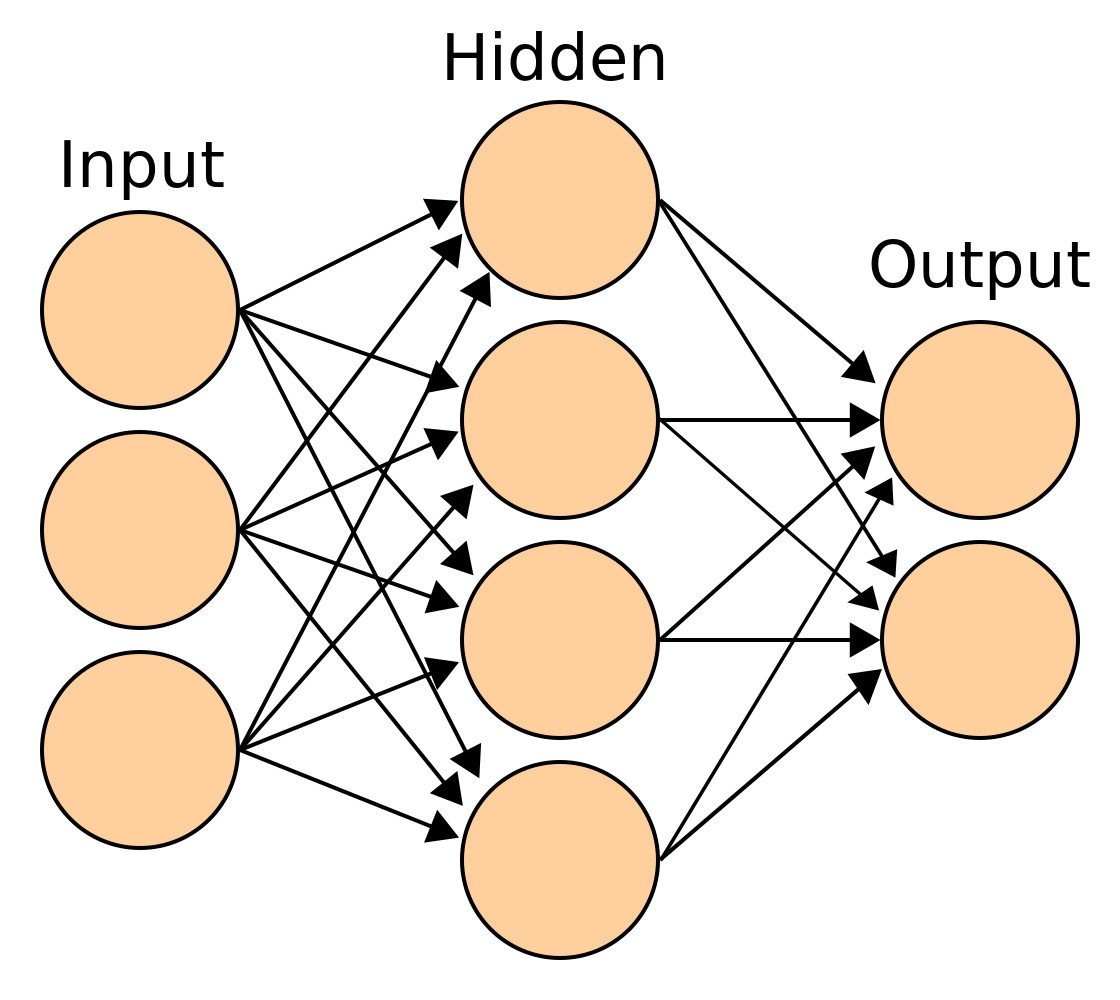
\includegraphics[width=0.95\linewidth]{images/Libro-img049.jpg}
  \begin{minipage}{\linewidth}
    \caption{Di en:User:Cburnett - Opera propriaQuesta grafica
vettoriale non W3C-specificata è stata creata con Inkscape., CC BY-SA 3.0,
\protect\url{https://commons.wikimedia.org/w/index.php?curid=1496812} }
  \end{minipage}
\end{wrapfigure}

Ma come funziona il deep learning? Proprio come il nostro cervello, creando neuroni e connessioni, ma questa volta
artificiali, completamente digitali. Come vediamo dall'illustrazione qui di fianco, abbiamo uno
strato di input, uno strato nascosto e, lo strato di output. Decidere quanti neuroni devono avere lo strato di input e
di output è molto semplice. Prendiamo il caso di un IA che deve capire da una foto, con rappresentato un numero scritto
a mano, di che cifra si tratta. L'immagine che verrà fornita all'IA è grande
8x8. Quindi avremo 64 neuroni nello strato di input. Il risultato che ci dovrà dare è un valore da 0 a 9, quindi in
totale 10 neuroni. Lo strato nascosto, o gli strati nascosti, siccome più sono, più possono apprendere in maniera
profonda e con un livello di astrazione più alto, hanno una difficoltà in più. Ad oggi non c'è un
modo per sapere quanti neuroni o strati nascosti impostare in un IA. La ricerca è ancora tanta, dove si fanno
tentativi, si usa l'esperienza, la sensibilità, l'intuito.

Ora dobbiamo addestrare questa rete che possa riconoscere i numeri scritti a mano. Inizialmente si attribuisce un valore
(peso) a caso ad ogni freccia che collega i vari neuroni. Poi gli si da in esame il primo elemento, che nel nostro caso
potrebbe essere la foto del numero 7. Siccome i valori delle connessioni sono stati messi a caso, il percorso in cui
verrà instradato questo input, arriverà in un neurone di output a caso, ad esempio il 5. Siccome i programmatori hanno
etichettato questa e, tutte le altre foto con il relativo risultato che dovrebbe fornire, la rete neurale,
automaticamente, sa che secondo le sue valutazioni è venuto fuori un 5 ma sarebbe dovuto essere un 7. Così, grazie alla
formula, che prende il nome di algoritmo di back propagation, l'IA ricalcola tutti i pesi delle
connessioni, in modo che la prossima volta che vedrà quell'immagine, saprà dare la giusta
risposta. Un 7 però, può essere scritto in infiniti modi, ogni persona lo scrive a modo suo e, anche la foto può essere
con una luminosità, inclinazione, orientamento, qualità diversa. Quindi mostrare ad una IA due immagini con un 7
equivale a mostrare due entità diverse e uniche che generano un relativo risultato, magari diverso tra loro. Così, se
mostriamo nuovamente una foto con un 7 alla nostra IA, potrebbe ancora sbagliare, ma grazie
all'algoritmo di back propagation, si avvicinerà ancora di un passettino alla creazione di un
giusto schema neurale, che gli consenta di classificare le immagini con una certa precisione. Al primo avvio della fase
di training, avremmo una percentuale di precisione dell'AI veramente bassa. Dopo cento esempi che
gli vengono mostrati sarà leggermente meglio. Si continua così, mostrando esempi, ricalcolando il peso delle
connessioni neurali, fino a quando la precisione di classificazione raggiunge un buon risultato. Alche il deep learning
come il machine learning consente di risolvere problemi di classificazione, regressione e clustering.

In realtà, la rete neurale non segue un solo percorso come detto in precedenza. L'ho scritto per
semplificare anche se virtualmente possiamo vederlo proprio così. In realtà vengono lanciati segnali su tutte le
connessioni e, tutti i neuroni si attiveranno ma con cariche diverse. Alla fine, nel nostro strato di output, avremo i
nostri 10 neuroni, tutti con un numero con la virgola compreso tra 0 e 1. Teniamo sempre l'esempio
del numero 7, la tabella di seguito mostra un risultato tipo.

\begin{flushleft}
\tablefirsthead{}
\tablehead{}
\tabletail{}
\tablelasttail{}
\begin{supertabular}{|m{2.291cm}|m{2.116cm}|}
\hline
Neurone di output &
Risultato del neurone\\\hline
0 &
0,01\\\hline
1 &
0,02\\\hline
2 &
0,08\\\hline
3 &
0,07\\\hline
4 &
0,09\\\hline
5 &
0,04\\\hline
6 &
0,05\\\hline
7 &
0,98\\\hline
8 &
0,03\\\hline
9 &
0,06\\\hline
\end{supertabular}
\end{flushleft}
Come vediamo per il neurone numero 7 abbiamo una probabilità del 98\% che il risultato sia proprio 7. Tutti gli altri
neuroni, danno comunque un risultato, ma con percentuali molto più basse.

Per entrare leggermente nel dettaglio per poi uscirne subito, possiamo guardare la seguente immagine.

\begin{figure}[H]
  \begin{minipage}{17cm}
    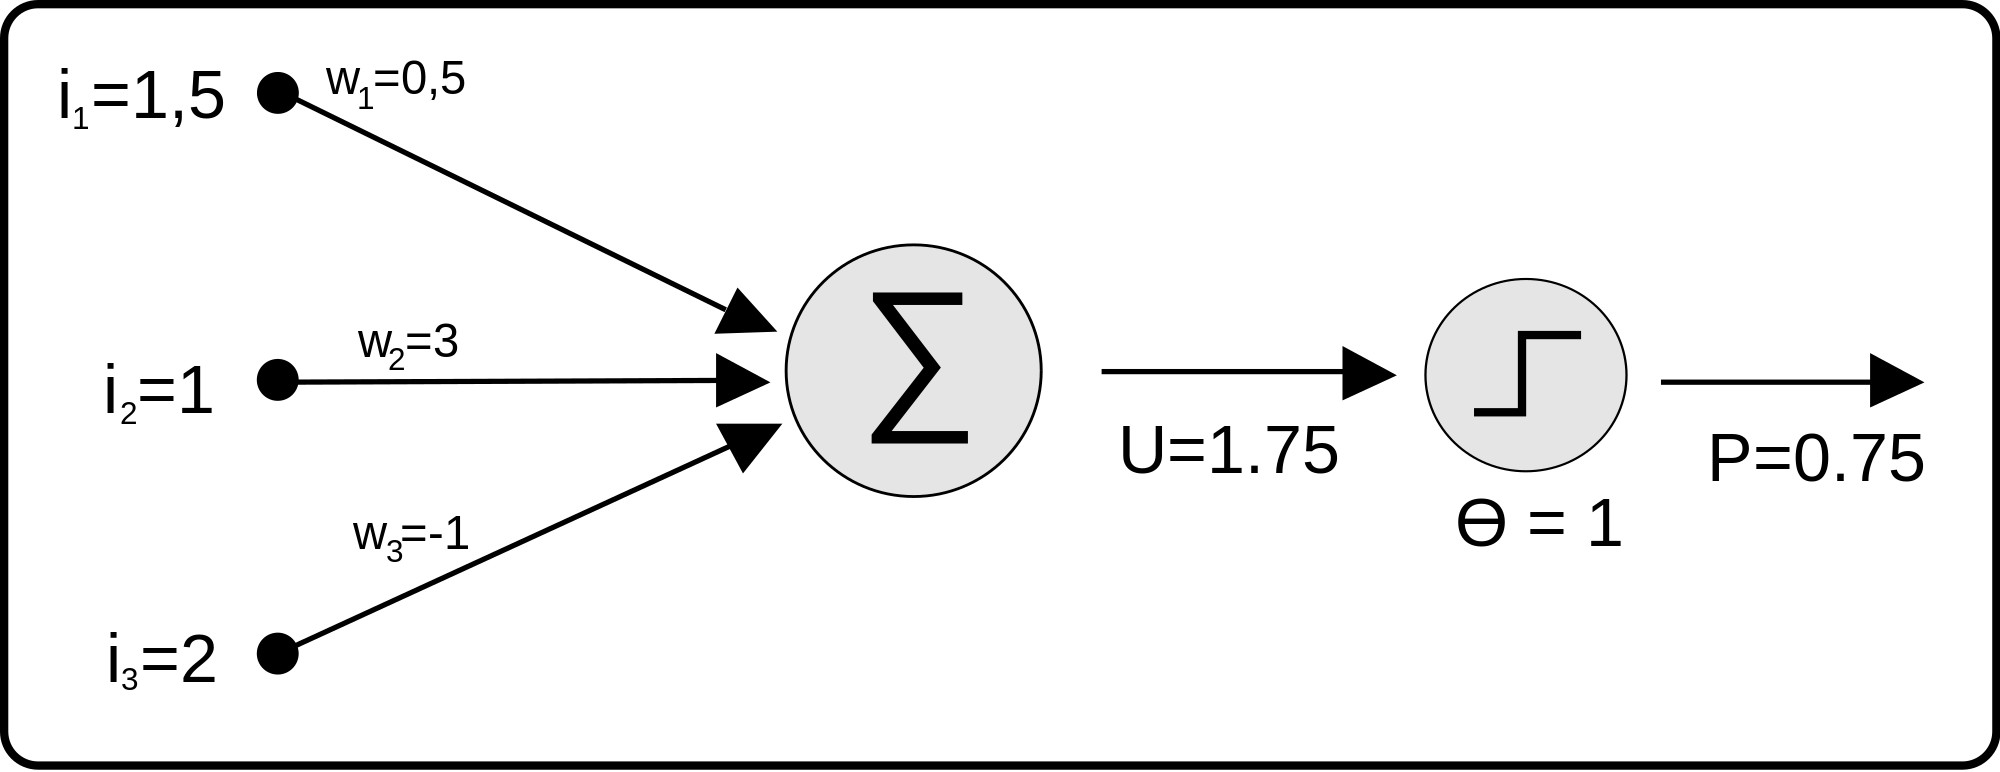
\includegraphics[width=17cm]{images/Libro-img050.jpg}
    \caption{Di DaniDF1995 - File:Neurone.artificiale.gif, CC BY 3.0, \protect\url{https://commons.wikimedia.org/w/index.php?curid=8279423}}
  \end{minipage}
\end{figure}

Questo è un esempio di tre neuroni (i1, i2, i3) collegati (con w1, w2 e w3) a un altro neurone.
Quest'ultimo riceve lo stimolo in input di tre neuroni e elabora un output. Ogni stimolo avrà un
peso diverso, maggiore se la connessione è forte. Possiamo vederla come una moltiplicazione tra i e w. Quindi avremo
1,5 * 0,5 = 0,75 poi avremo il secondo neurone con 1 * 3 = 3 e infine il terzo con 2 * -1 = -2. Il neurone $\Sigma $
sommerà i risultati, quindi 0,75 + 3 -2 = 1,75. Se la somma supera una certa soglia, il neurone attiverà la sua uscita.
Per cui è possibile che due neuroni instaurino una connessione più forte rispetto agli altri, creando dei “percorsi
preferenziali”. Ma è sbagliato pensare che la rete finisca col produrre un unico percorso di connessione: tutte le
combinazioni infatti avranno un certo peso, e quindi contribuiscono al collegamento input/output.

Se guardassimo dentro una rete neurale, non riusciremmo a capire, per via della sua complessità, per quale logica certe
connessioni siano più forti di altre. Però possiamo sapere che funziona con un certo grado di precisione, anche se non
sapremo spiegarcelo. 

Un caso iconico è stato quello di AlphaGo un IA creata da Google per giocare a Go. Go è un antichissimo gioco da tavolo,
come gli scacchi, ma con una griglia molto più ampia, senza uno schieramento iniziale, e senza limiti di “passi” che
possono fare le pedine. Lo scopo è accerchiare l'avversario coprendo un area più ampia possibile
di gioco. L'Ibm creò nel 1997 un'IA capace di battere il campione mondiale di
scacchi e, fu stato un traguardo eccezionale, per via degli infiniti schemi che si possono presentare in una partita di
questo gioco. Per Go, le possibilità sono ancora più infinite. Nel 2015 AlphaGo sconfisse 5 a 0 il campione europeo e,
nel 2016 il campione mondiale per 4 a 1. AlphaGo siccome non ha avuto alcuna influenza culturale e emotiva durante il
gioco, riusciva a fare delle mosse che per un essere umano sarebbero state definite completamente assurde, sbagliate
addirittura. Man mano che il gioco si sviluppava, però, si vedeva che quelle mosse erano necessarie e decisive per la
sua strategia di gioco inumana, incomprensibile ma efficace.


\bigskip

Super riassunto: l'intelligenza artificiale sa prendere decisioni, non perché consapevole del suo
ragionamento e, dopo un'attenta analisi fatta da riflessioni, valutando la situazione. Ma perché
in base alla grandissima mole di esempi simili che ha visto, sa che statisticamente la sua decisione sarà probabilmente
giusta. Senza sapere il perché.

\subsection{Obsolescenza programmata}
L'obsolescenza programmata è una strategia economica che definisce la durata di un prodotto in modo
da limitarla. Il prodotto dopo un certo tempo di utilizzo smette di funzionare oppure diventa semplicemente superato
rispetto ai nuovi modelli anche se non presentano interessanti caratteristiche aggiuntive rispetto a quello vecchio.

\begin{wrapfigure}{i}{9cm}
  \centering
  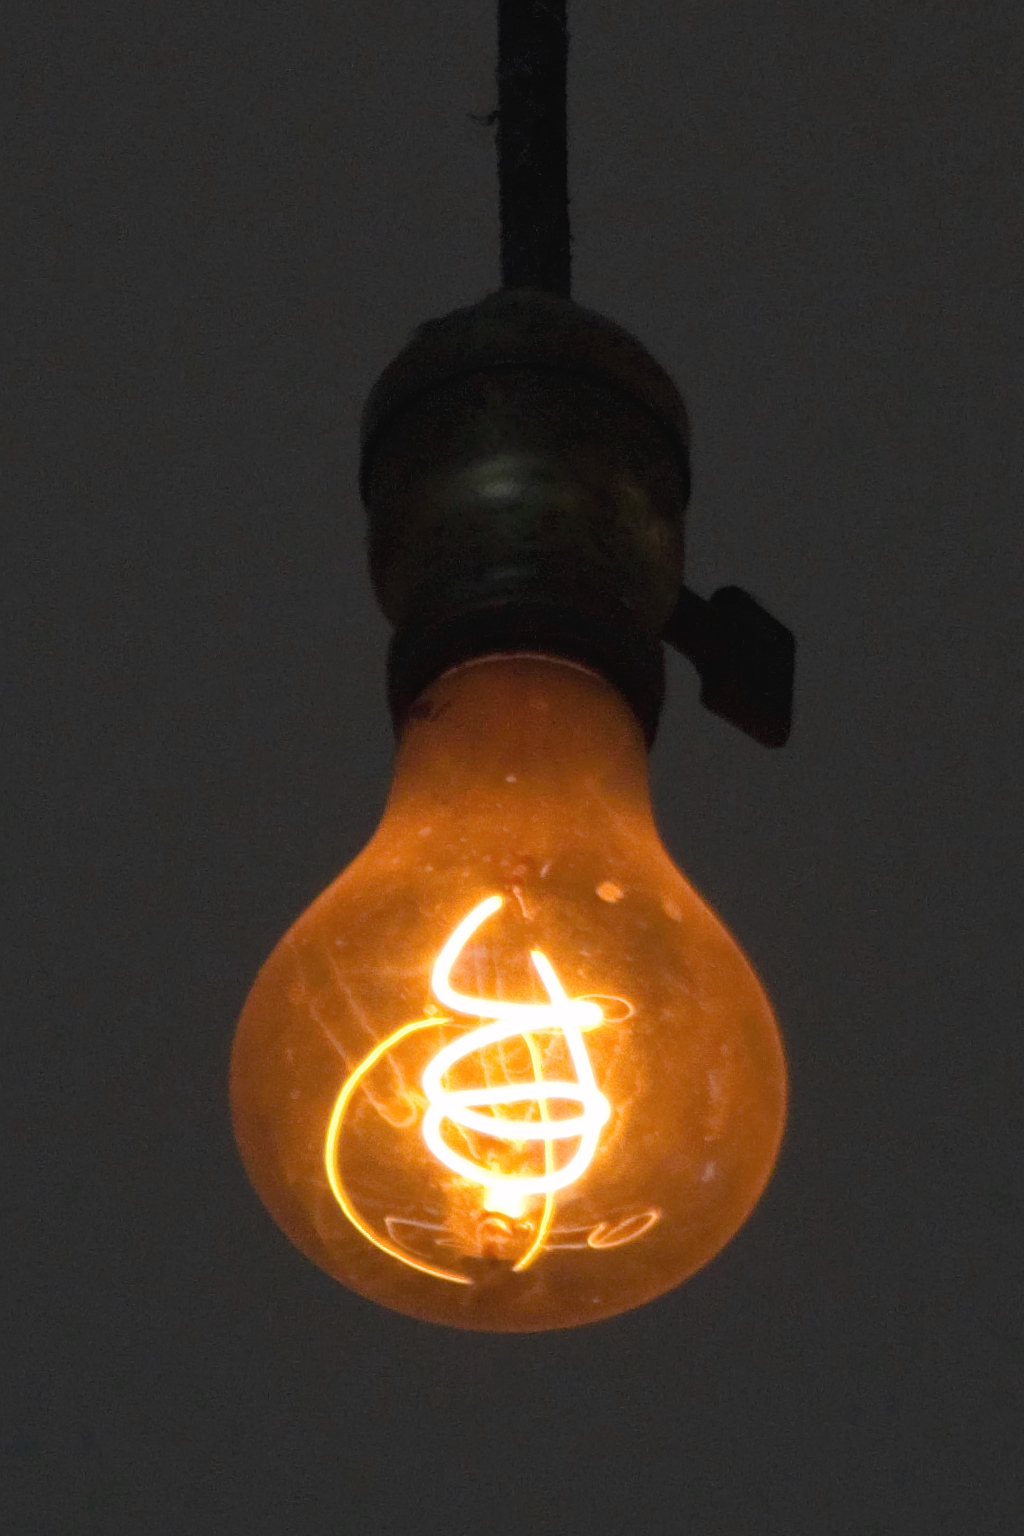
\includegraphics[width=0.95\linewidth]{images/Libro-img051.jpg}
  \begin{minipage}{\linewidth}
    \caption{Lampadina centenaria nella caserma dei vigili del
fuoco di Livermore-Pleasanton California. Di LPS.1 - Opera propria, CC0,
\protect\url{https://commons.wikimedia.org/w/index.php?curid=29802905}}
  \end{minipage}
\end{wrapfigure}

Il primo prodotto a cui è stata applicata questa strategia sembra essere stata la lampadina. Quante volte vi sarà
capitato anche a voi di cambiare una lampadina? Fino a poco tempo fa, con le lampadine a incandescenza non era raro che
una si bruciasse e andasse sostituita. Eppure, a Liverpool in California esiste una lampadina in una caserma dei
pompieri che è accesa dal 1901, quindi, tecnologicamente, \ possibile creare una lampadina praticamente eterna. Nel
natale del 1924 \ a Ginevra il \ Cartello Phoebus decise che le lampadine dovevano durare mediamente 1000 ore, multando
i produttori che superavano le 1500. Come mai presero questa decisione? Con la rivoluzione industriale e
l'introduzione della produzione in serie grazie a macchinari capaci di lavorare molto più veloce
di un gruppo di persone. Questo ha potuto permettere un abbassamento dei costi dei prodotti, ma nonostante questo, la
produzione era talmente efficiente che si aveva un offerta molto più alta della richiesta di allora. Nel 1929 quando
l'America sprofondò nella grande depressione venne scritta per la prima volta da Bernard London
una proposta per rendere obbligatoria l'obsolescenza programmata come strategia per far riprendere
l'economia. Questa manovra resa obbligatoria e alla luce del sole avrebbe probabilmente portato a
disordini così venne ignorata. L'idea però rimase latente per anni e nel dopoguerra riaffiorò in
maniera più subdola. Uscì dalla porta nel 1929 e rientrò dalla finestra negli anni 50. Il designer statunitense Brooke
Stevens non obbligò le persone a comprare i suoi prodotti, ma indusse il desiderio grazie al marketing e al design
seducendo il consumatore a volere il prodotto più nuovo, più moderno, più bello. Nelle persone
dev'esserci l'idea che quello che hanno, anche se funziona, a un certo punto
non lo vogliono più, perché desiderano la versione più moderna solo perché è più moderna. Non sono obbligati ma indotti
e sedotti a farlo. Quando l'unico accorgimento adottato per rendere obsoleto un prodotto prima del tempo è la
pubblicità si può parlare di obsolescenza percepita o
simbolica\endnote{\protect\url{https://it.wikipedia.org/wiki/Obsolescenza\_programmata} }. 

"L'instillare nell'acquirente il desiderio di comprare qualcosa di appena un po' più nuovo e un po'
prima di quanto sia necessario"\endnote{\protect\url{https://mam.org/collection/archives/brooks/} }.

Questo è alla base del consumismo. L'economia che dovrebbe essere orientata al soddisfacimento dei
desideri dell'uomo diventa invece orientata all'economia stessa, alla
crescita non per il progresso ma solo per la crescita in sé. Ma in un mondo con risorse finite la crescita infinita
proposta dal capitalismo e dal consumismo diventa insostenibile e intrinsecamente destinata al collasso.

\begin{wrapfigure}{i}{9cm}
  \centering
  
\includegraphics[width=0.95\linewidth]{images/Libro-img052.jpg}
  \begin{minipage}{\linewidth}
    \caption{Frame esdtratto dal documentario {\textquotedbl}il
complotto della ampadina{\textquotedbl} dove si mostra la resistenza di una calza di nylon in grado di trainare un auto
senza rompersi}
  \end{minipage}
\end{wrapfigure}

Abbiamo numerosi esempi, come le calze di nylon ideate dall'azienda chimica du'Ponts nel 1940 che
inizialmente erano così resistenti da poter trainare un auto, ma una volta che tutte le persone avessero comprato
abbastanza calze per la settimana o lampadine per illuminare casa, non avrebbero più venduto il prodotto portando al
conseguente licenziamento degli operai fino al fallimento della fabbrica. Così decisero come per la lampadina, di
ridurre la robustezza e la durata delle calze. Non sappiamo cosa succederebbe se si decidesse di creare prodotti a
lunga durata. Gli unici esempi che abbiamo li troviamo in stati che sono stati comunisti come Russia e Germania
dell'est. In quanto non esisteva il libero mercato l'obsolescenza programmata
non aveva senso di esistere in quanto tutto veniva gestito dallo stato non c'era la preoccupazione
che una singola azienda potesse fallire, così lo scopo non diventava quello di sopravvivenza economica ma di creare un
prodotto valido. Le lampadine, elettrodomestici come frigoriferi prodotti dalla Germania dell'est
sono funzionanti ancora oggi. Con la caduta del muro di Berlino progressivamente e del comunismo nei paesi
dell'est il consumismo dilagò facendo sparire questi produttori.

Un esempio dei giorni nostri che ripetutamente ha fatto scandalo è stata la Apple. Nel 2003 è stata chiamata in causa
per i suoi iPod. Durante il processo è emerso che le batterie erano state disegnate per durare circa 18 mesi.
Dopodiché, siccome l'azienda non vendeva le batterie singolarmente, consigliavano di sostituire
interamente il prodotto che non era nemmeno a buon mercato. Al termine della causa arrivarono ad un accorto che portò
Apple a estendere a due anni la garanzia dei suoi prodotti e a fornire batterie di ricambio.

Mentre in passato l'obsolescenza programmata richiedeva uno studio chimico per definire il ciclo di
vita di un prodotto, oggi, con la diffusione dell'elettronica le cose si sono semplificate. Per
esempio basta non fornire più gli aggiornamenti per le vecchie versioni di un dispositivo o rendere le applicazioni
incompatibili. O creare degli aggiornamenti che riducano la durata della batteria com'è stato
condannato dall'Antitrust per aziende come Apple a Samsung. Apple è un esempio iconico. Prodotti
con un bellissimo design, pubblicità che sono passate alla storia\endnote{\protect\url{https://www.youtube.com/watch?v=2zfqw8nhUwA}
}, l'uscita di nuovi prodotti con cadenza regolare anche senza significativi cambiamenti.

Nel documentario “Il complotto della lampadina”\endnote{\protect\url{https://www.youtube.com/watch?v=kjI8ETxThDw} } viene raccontata
la storia di Marcos che ha un guasto alla sua stampante Epson stylus c44 series. Sottopone la sua stampante ad alcuni
centri d'assistenza che gli spiegano che tra i pezzi di ricambio e la manodopera il prezzo della
riparazione supererebbe le 100 euro e, non conviene siccome esistono stampanti nuove che ne costano 30. Marcos però
decide di ripararla e leggendo la documentazione scopre che all'interno esiste un chip eeprom il
cui suo unico compito è contare le stampe e bloccare la stampante una volta raggiunte le 1800 pagine, anche se il
prodotto è ancora perfettamente funzionante. Continuando le sue ricerche scopre che un programmatore russo ha creato un
programma\endnote{\protect\url{http://ssclg.com/epson.shtml} } che riesce ad azzerare questo contatore. Marcos prova questo
programma e senza spendere un centesimo con suo grande stupore riesce a far ripartire la stampante. Questo è un ottimo
esempio di come sia facile utilizzare questa politica nei prodotti elettronici.

Werner Scholz, direttore dell'associazione tedesca dei costruttori di elettrodomestici, ha espresso dubbi sulla
lungimiranza dell'obsolescenza programmata in quanto, gli acquirenti delusi di un prodotto migreranno poi verso le
aziende capaci di creare prodotti durevoli nel tempo. A meno che ci sia un controllo di lobbi che regolamentano la
produzione di un prodotto come nel caso del cartello Phoebus. Però, proprio le lampadine stesse sono riuscite ad uscire
da questa logica grazie a Warner Philips che mise in commercio le lampadine a LED della durata di 25 anni, costringendo
tutti gli altri produttori, per reggere la competizione del mercato a creare prodotti con la stessa tecnologia e con la
stessa qualità.

Un ulteriore problema legato all'obsolescenza programmata è il conseguente aumento di rifiuti. In
particolare i rifiuti tecnologici vengono poi buttati in paesi dell'Africa come il Ghana. Questa
pratica ufficialmente illegale ma se vengono fatti passare come prodotti di seconda mano per colmare il divario
tecnologico tra i paesi del terzo mondo e i paesi occidentali allora è consentito. Il problema è che questi prodotti
non sono utilizzabili, non funzionano e, vengono riversati in queste immense discariche a cielo aperto dove le persone
estraggono i metalli contenuti negli elettrodomestici. Per farlo però mettono in serio pericolo la loro salute,
correndo il rischio di tagliarsi, prendere infezioni e inalare i fumi prodotti dalle plastiche che bruciano nel
tentativo di estrarre i metalli contenuti al loro interno.

La questione dell'obsolescenza programmata può sembrare sbagliata senza nessuna discussione, un
sopruso a discapito del popolo. Purtroppo però, senza di essa potremmo avere problemi ben più gravi. Questa strategia
consente mantenere alti i consumi e la produzione, di conseguenza consente di dare lavoro a più persone. Se non ci
fosse le fabbriche inizierebbero a chiudere una volta che tutta la popolazione dispone di quel bene. Altre questione è
che la durabilità, di questi tempi, non è un valore così fondamentale. Tanti di noi, se avessero uno smartphone eterno,
comunque lo cambierebbero per il modello più nuovo nel giro di un anno o due. Sicuramente però non possiamo accettare
tanti degli esempi visti fin ora. Una scelta polarizzata su un estremo o sull'altro andrebbe a
penalizzare troppo produttore o consumatore, quindi anche qua, bisogna trovare la via di mezzo, mantenendo
l'obsolescenza programmata ma con leggi che garantiscano standard di durabilità, possibilità di
sostituire i pezzi principali e garanzie estendibili. Ci sono però anche tantissimi filosofi e intellettuali che
sostengono che invece sia fattibile attuare una decrescita che non comporti riduzioni del tenore di vita, per eliminare
l'obsolescenza programmata. 

Non so quale sia la strada giusta, ma in questa sezione di curiosità rilancio con un'altra
possibilità, il paradismo.

\subsection{Paradismo}
Il Paradismo è un sistema politico simile al comunismo, ma senza proletariato. In un sistema paradista, i robot
sostituiscono la forza lavoro umana. Tutti i beni e i servizi (tra cui produzione e raccolta del cibo, consegna a
domicilio automatica, robot-chirurghi, ecc..) verranno nazionalizzati renderanno il denaro obsoleto, dal momento che
sarà tutto gratuito. In questo sistema i politici eletti lavoreranno mossi da un sincero desiderio di utilità verso
l'Umanità in quanto non godranno di benefici economici. Così, invece di lavorare unicamente per guadagnare denaro, gli
esseri umani potranno lavorare su ciò che amano: creare, studiare, ricerche, opere d'arte, musica, sviluppo
personale\endnote{\protect\url{https://it.paradism.org/page.php?8} }.

\subsection{Paradosso di Fermi}
Siamo tutti d'accordo che nell'infinità dell'universo e
dei suoi relativi pianeti e stelle non possiamo essere le uniche forme di vita nell'universo. Ma
se ci sono così tante civiltà evolute, perché non ne abbiamo ancora ricevuto le prove, come trasmissioni radio, sonde o
navi spaziali?

Questa è la domanda che fa nascere il paradosso di Fermi (attribuito al fisico Enrico
Fermi)\endnote{\protect\url{https://www.ted.com/talks/stephen\_webb\_where\_are\_all\_the\_aliens/transcript?language=it} }. Francis
Drake ha così creato l'omonima equazione di Drake per stimare la probabilità di quante forme di
civiltà aliene possano esistere. Il problema è che non conosciamo i valori di alcuni parametri come ad esempio la
probabilità che la vita o l'intelligenza si sviluppino.

In uno studio della Oxford University\endnote{\protect\url{https://arxiv.org/pdf/1806.02404.pdf} } hanno tentato di dare una risposta
risolvendo più volte l'equazione utilizzando dati casuali, sempre diversi, presi da pubblicazioni scientifiche.
Provando diverse volte l'equazione e ottenendo zero come risultato hanno dimostrato che non
esistono altre forme di vita intelligente nel nostro universo osservabile. Quando parliamo di forme di vita evolute o
intelligenti stiamo indicando organismi capaci di uscire dal loro pianeta fisicamente con navicelle o virtualmente con
segnali di vario tipo come onde radio. Abbiamo citato diverse volte i fenomeni controintuitivi, dove il nostro
ragionamento, in maniera comprensibile, razionale e giusta ci da un risultato che però la freddezza della fisica e
della matematica dimostrano errato. Siamo abituati infatti a vedere sul nostro pianeta terra
un'infinità di modi in cui la vita ha saputo svilupparsi, in questo angolo minuscolo e
insignificante dello spazio portandoci così a pensare che in altre galassie potrebbe essersi verificato lo stesso
fenomeno. Ma le condizioni che la vita si sviluppi fino a portare alla luce organismi complessi è davvero particolare,
molto ma molto più difficile di quello che ci immaginavamo. La vita per svilupparsi deve superare diversi \ “filtri”,
che sono dati dall'ambiente, l'evoluzione dell'ambiente,
continue minacce che possono venire dall'universo o dal pianeta stesso, per esempio, nel nostro
caso, anche avere un satellite, di particolari dimensioni ha giocato un ruolo cruciale. La Luna esercita un attrazione
sulla terra che gli consente di mantenere un asse più stabile, in modo da non avere inverni troppo freddi e estati
torride, regola le maree, e la stabilità dei poli. Un delicato equilibrio che non avremmo senza Luna o se avesse avuto
dimensioni diverse. Ci sono probabilità molto più alte di essere le uniche forme di vita così complesse
nell'universo e, il fatto che esista anche un solo caso come il nostro in tutto lo spazio è in
realtà un vero miracolo. In tanti hanno provato a svolgere l'equazione di Drake ma sempre con lo
stesso risultato. Il paradosso di Fermi ora infatti sta spostando la sua attenzione da, inizialmente dare una stima
delle vite potenziali nello spazio, a ora che sta cercando di capire le spiegazioni del perché non esistano altre
civiltà evolute. Esistono tante teorie: che gli alieni siano {\textquotedbl}in letargo{\textquotedbl}, sepolti sotto
croste di ghiaccio, bloccati da ostacoli vari ecc... Tra le teorie più accreditate si pensa che gli alieni si siano già
esistiti, quindi, modificando la variabile “tempo” troviamo una probabilità concreta che più civiltà evolute si siano
mostrate nello spazio, ma mai contemporaneamente nello stesso periodo storico. Di riflesso è nata la teoria che se
cercasse di nascere un'altra forma di vita mentre è in essere una più evoluta,
quest'ultima, nel tentativo di scoperta e gestione dell'energia prodotta
dalla sua stella, finirebbe per distruggere le forme di vita minori senza rendersene conto. Un po' come la costruzione
di un palazzo che ucciderebbe migliaia di insetti senza farlo apposta. Il paradosso di Fermi quindi ribalta
completamente, usando la matematica, l'idea che avevamo sulla probabilità di forme di vita aliene
nell'universo. Questo deve far riflettere su come stiamo usando il nostro pianeta, se arrivassimo
a mezza notte nell'orologio dell'apocalisse lasceremmo
l'universo completamente solo, senza forme di vita complesse. Quando mi capita di parlare di
questo paradosso con le persone noto sempre molta resistenza, sottolineandomi quanto sia immenso
l'universo e di conseguenza le probabilità che una civiltà più evoluta della nostra possa essersi
sviluppata, ma questo in realtà è ben noto ai ricercatori e, questa variabile è stata la prima ad essere presa in
considerazione.

Alla domanda posta all'inizio: Dove sono tutti? Qualcuno potrebbe rispondere che esistono numerose
testimonianze anche foto e video dell'esistenza aliena. Anni fa ricordo che
c'era una trasmissione televisiva dove una persona riusciva ad analizzare le foto per capire se
fossero false o possibili, ovviamente la certezza di un vero non si può avere, magari la persona che ha creato il falso
è stata più brava di quanto noi sappiamo scoprirli. Questa persona che scovava i falsi si chiama Pablo Ayo, gli ho
scritto anni fa diverse volte, tramite il suo sito internet, ma senza successo. Volevo chiedergli se sapeva darmi una
percentuale di quanti falsi girano per il web. Ho così cercato di fare io questo esperimento prendendo un po' di
immagini a caso su internet e analizzandole. Il risultato è che l'80\% era sicuramente un falso e
l'altro 20\% troppo sfocato per un analisi. Quindi vuol dire che ottimisticamente
l'80\% delle prove che abbiamo sugli aliene sono falsi, più realisticamente possiamo dire che il
99,9\% di foto e video che abbiamo visto sono falsi.

\begin{figure}[H]
  \begin{minipage}{17cm}
    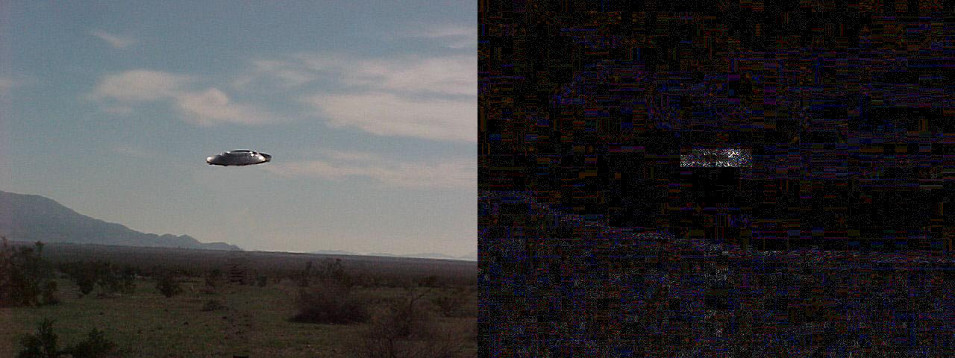
\includegraphics[width=17cm]{images/Libro-img053.jpg}
    \caption{Esempio di come i filtri possono rilevare un falso. Nell'immagine di destra si vede chiaramente un elemento estraneo applicato in un secondo momento all'immagine originaria.}
  \end{minipage}
\end{figure}

Esistono però dei video diffusi dall'aeronautica statunitense e non solo, dove vengono inquadrati
degli UFO. Questi video sono certificati come autentici dall'aeronautica stessa, a dispetto di
quanto si possa pensare circa l'atteggiamento dei governi impegnati a nascondere la verità. Questo
non significa che stiano ammettendo la presenza di alieni, ma solo di oggetti non identificati. Secondo Paolo
Attivissimo, fra i più noti debunker del settore e socio emerito del Cicap, (Comitato italiano per il controllo delle
affermazioni sulle pseudoscienze) il dipartimento della Difesa americano, stanco di tollerare azioni di spionaggio o
sorveglianza da parte di altre potenze, stia cercando il modo più accorto per farlo sapere. Questo perché, dal punto di
vista militare, sarebbe un segno di debolezza ammettere che droni di altre potenze sorveglino le proprie navi o violino
uno spazio aereo. Abbatterli innescherebbe invece un incidente diplomatico. Spesso gli incidenti militari sono stati
coperti lasciando credere si trattasse di qualche intrusione extraterrestre, in modo da evitare che indagini più
approfondite che scoprissero attività poco convenienti o operazioni segrete. Altre volte invece è capitato, come
durante lo sviluppo dell'aereo F-117 Nighthawk, che qualcuno avvistasse delle strane forme
triangolari in cielo. Questo perché né i piloti né chi ha redatto il rapporto è a conoscenza dei piani di sviluppo
segreti del proprio governo, solamente pochissime persone ne sono a conoscenza. In Italia sono stati censiti circa
30mila casi di avvistamenti di oggetti non identificati. Ma quelli potenzialmente veri sono tra il 3 e e il 5\% dei
casi. Dico potenzialmente perché anche quelli potrebbero essere falsi: nel 1990 in Belgio è stata scattata una foto di
un oggetto triangolare con sfere luminose e giudicata vera dal dal ministero della Difesa e, 11 anni dopo è stata
rivelata come un falso dallo stesso autore.


\bigskip

Secondo il debunker potrebbe esserci una correlazione fra i momenti di incertezza politica e di paranoia nazionale
seguita da comparsa di avvistamenti ufologici.“Spesso, si proietta la paura dello straniero,
dell'estraneo, dell'invasore su qualcosa di analogo. La cinematografia
occidentale degli anni 50 non a caso è zeppa di marziani, dischi volanti e guerre dei mondi. Che
cos'era L'invasione degli ultracorpi se non la metafora della minaccia
comunista (con tanto di indottrinamento, di lavaggio del cervello)? Oggi ho l'impressione che da
una parte ci possa essere una correlazione fra il sentimento collettivo di insicurezza e
l'esigenza di sfogarlo in maniera socialmente
accettabile”\endnote{\protect\url{https://www.wired.it/scienza/spazio/2021/06/04/ufo-uap-rapporto-stati-uniti/}.}


\bigskip

Precedentemente quando abbiamo parlato di complotto abbiamo visto come tutto comunque sia contestabile, anche davanti
alle prove, basta decontestualizzare, travisare, mostrare solo una parte, impostare i grafici un un certo modo,
sfruttando le deformazioni della realtà ecc… Io so solo che mi trovo a dover scegliere tra articoli sul web con
immagini probabilmente false e pubblicazioni scientifiche che dimostrano matematicamente, che non esistono altre forme
di vita intelligente nel nostro universo osservabile. Io mi sento di credere solo al metodo scientifico che è
l'unica struttura che reggendosi tramite una rete di ricercatori anche indipendenti, di
conseguenza non soggetta ai poteri forti, può validare tramite la comunità scientifica una teoria oppure
no\endnote{\protect\url{https://www.focus.it/scienza/spazio/gli-alieni-non-esistono} }.


\bigskip

Se volete approfondire ci sono questi due video molto popolari su youtube:

\protect\url{https://www.youtube.com/watch?v=sNhhvQGsMEc}

\protect\url{https://www.youtube.com/watch?v=1fQkVqno-uI}


\bigskip

Allo stesso modo troviamo una ricerca dell'Università di Nothingam, che modificando
l'equazione di Drake, stimano che nella via lattea ci possano essere 36 civiltà
extraterrestri\endnote{\protect\url{https://www.wired.it/scienza/spazio/2020/06/18/via-lattea-30-civilta-extraterrestri/} }
\endnote{\protect\url{https://iopscience.iop.org/article/10.3847/1538-4357/ab8225} }.

Anche in questo caso dove sta la verità? Non possiamo saperlo e nessuno potrà dircelo con certezza, possiamo fare
ipotesi e adottare quella che ci piace di più non perché sia vera ma perché ci piace credere così.
L'unica verità è che a volte dobbiamo accettare che non possiamo saperlo, che non possiamo
appagare questo nostro desiderio di ordine.


\bigskip

\subsection{Droga}

\begin{wrapfigure}{i}{4.972cm}
\includegraphics[width=4.972cm,height=7.287cm]{images/Libro-img054.jpg}
\caption*{Di Mpv\_51 at English Wikipedia - Transferred from English Wikipedia, Pubblico dominio, \protect\url{https://commons.wikimedia.org/w/index.php?curid=546164} }
\end{wrapfigure}

A Ginevra, in Svizzera, è stato sviluppato un metodo unico per aiutare i tossicodipendenti. A fine degli anni 80 Ginevra
si è trovata ad affrontare una crisi sanitaria legata al consumo di eroina e dell'HIV. Le due
strade percorribili al fine di risolvere questo problema sono due, liberalizzazione o repressione. Ginevra ha scelto la
prima strada, in una maniera più attiva di altri esempi che abbiamo parsi per il mondo. Hanno abbandonato
l'idea romantica e utopica di rimuovere la droga dalla società, in quanto ancora nessuno al mondo
c'è riuscito. Il loro obiettivo non è rimuovere la droga ma tutte le problematiche che ruotano
attorno ad essa come violenza e salute. Così è stata adibita una struttura dove gli vengono fornite siringe nuove,
preservativi e assistenza medica. Come abbiamo visto l'ambiente e la genetica forma noi stessi
molto più di noi stessi. Così anche noi saremmo potuti essere dei tossicodipendenti e, la gente che ha bisogno di
aiuto, lo deve ricevere. Così a Ginevra lo stato a deciso di fornire l'eroina a chi ne è
dipendente. L'eroina èstata inventata dalla Bayer, la stessa azienda che produce
l'aspirina, a fine dell'800 e veniva data ai bambini per dolori ai denti,
diarrea, malattie respiratorie. Veniva esportata in 23 paesi di tutto il mondo. Quando si resero conto della fortissima
dipendenza che dava il farmaco venne ritirato dal commercio lasciando però un sacco di persone dipendenti che
continuarono a ricercarla sul mercato nero, dove però la purezza arriva al massimo al 15\% il resto è tutto “taglio”
tra cui può essere fatto con pezzi di intonaco, terra, calmanti. L'eroina pura se iniettata
correttamente e con un giusto dosaggio, essendo un medicinale, non da problemi, al massimo un po' di costipazione. La
differenza sta nel non fare differenza tra droga, intesa come sostanza e dipendenza. Non sto dicendo che
l'eroina sia buona, da moltissima dipendenza ma per l'organismo, se è pura, è
meno tossica dell'alcol o delle sigarette. Anzi, forse la sigaretta da anche uno pochino più di
dipendenza siccome l'effetto dura solo 15 minuti e poi si è pronti idealmente a farsene
un'altra. Con l'eroina invece, siccome l'effetto è molto
più potente e dura qualche ora si può ridurre il consumo a una volta al giorno. Fa strano, mi rendo conto, lo stato
però non rende dipendenti le persone da questa sostanza, quando arrivano in questi centri lo sono già. Rispetto alla
situazione in cui arrivano, ovvero dipendenti e con rischio di prendere infezioni e di logorare il loro organismo, loro
cercano di rimuovere tutti questi effetti, tranne la dipendenza. Ovviamente se non hai mai fatto uso di eroina questi
centri non possono dartela. I requisiti sono l'aver provato almeno due trattamenti in precedenza
che poi però non sono riusciti. I trattamenti possono essere la disintossicazione, il metadone o altre sostanze. I
pazienti raccontano che prima si facevano anche sette o otto volte al giorno, ora, con l'eroina
pura basta una sola volta. Se una persona fa uso di una sostanza otto volte al giorno, tutta la giornata è impiegata
nella ricerca della droga non lasciandogli tempo per fare altro. Riducendo il consumo a una sola volta invece possono
andare a lavoro e avere il resto della giornata per condurre una vita normale. Questo è solo uno dei tanti benefici
psicologici, gli altri sono: diminuzione criminalità, diminuzione dell'HIV e di altre infezioni,
miglioramenti della salute mentale. Inoltre, anche se allo stato non interessasse della salute dei tossicodipendenti ma
solo di spendere meno soldi, questa sarebbe la scelta giusta, siccome costa meno pagare l'eroina
che pagare le spese mediche per curarli quando arrivano troppo malati, con l'HIV o altre
infezioni. La società è piena di droghe più dannose e che danno dipendenza, come l'alcol, il
tabacco, le medicine, antidolorifici, psicofarmaci. Non è vero che una cosa legale fa meno male di una non legale.
Muoiono più persone per sigarette e alcol che per l'eroina. Inoltre i paesi che hanno legalizzato
le droghe non hanno avuto un aumento di consumo, anzi, una leggera
diminuzione\endnote{\protect\url{https://www.iene.mediaset.it/video/viviani-curarsi-con-l-eroina\_66062.shtml} }. Qualcuno dice che
la droga rovina i nostri figli, ma proprio per questo andrebbe legalizzata. Se prendiamo ad esempio le sigarette, un
minorenne non può comprarle, l'unica cosa che può fare è recarsi ad un distributore automatico e,
con la complicità di un adulto, che gli presterà un documento potrà acquistarle. Nel caso
dell'alcol è più difficile ancora, siccome il controllo dell'identità è fatto
sempre da un essere umano e non da una macchina. Anche qua, ovviamente un minorenne può accedere a questa sostanza, ma
solo con l'approvazione di un adulto. Nel caso della marijuana un minorenne può comprarla senza
nessun vincolo o complicità di nessun adulto. Quindi con il sistema attuale i minorenni hanno un accesso più complicato
a sostanze controllate e un accesso facilitato a sostanze di cui non c'è controllo della qualità.

\subsection{Pedofilia}
Vivere con certezze su tutto, sicuramente ci da un ordine e serenità ma è un illusione. Uno degli scopi di questo libro
è proprio questo. Non avere certezze, mettere in discussione tutto e, vedere che quello che è vero per me magari non lo
è per te e viceversa. Però ci sono delle cose su cui possiamo dire tutti, all'unanimità, con certezza che sono giuste o
sbagliate no? Per esempio, i pedofili sono sbagliati! Su questo siamo tutti d'accordo e non ci piove! O forse no?
Discorso spinoso...

Ho trovato interessante questo
articolo\endnote{\protect\url{https://www.vice.com/it/article/aev5vj/un-pedofilo-si-rivolge-ai-suoi-detrattori} } dove viene
intervistato Todd Nickerson, 43 anni, vergine. Fa il grafico, vive solo in una roulotte e, per molto tempo è rimasto
chiuso nella sua camera, isolato, perché ha un segreto: è attratto dai bambini.

Nickerson è un pedofilo, prova pulsioni sessuali per i bambini a cui però non ha mai dato seguito, né lo farà mai in
futuro.

Secondo alcune stime i pedofili sono tra lo 0,5\% e il 2\% della popolazione, ma tra i reati di pedofilia tra il 40\% e
il 75\% non sono compiuti da pedofili. Queste persone, attratti da adulti, usano i bambini in sostituzione di un
partner sessuale adulto.

{\textquotedbl}Ci sono persone che sanno di avere pulsioni sessuali nei confronti dei bambini, e che per tutta la loro
vita non fanno niente, non scaricano pornografia infantile, non infrangono la legge,{\textquotedbl} dice James Cantor,
uno psicologo e studioso della sessualità.

I media così definiscono pedofili tutte le persone che commettono reati sessuali su minori alimentando questa
confusione.

Spesso alle spalle di adulti che sentenziamo come malvagi, anche al di fuori della pedofilia, troviamo storie di bambini
innocenti e senza colpe che hanno subito dei traumi. Anche Nickerson, racconta di essere stato molestato quando aveva
sette anni da un amico di famiglia, identificandosi in quella persona siccome era molto gentile e mostrava interesse
per lui. Nickerson si accorse di avere desideri diversi dagli altri quando aveva 13 anni, quindi, quando ancora era lui
stesso un bambino. I suoi coetaei dicevano di essere attratti dalle ragazzine più sviluppate mentre lui si accorse, a
casa dei nonni, quando arrivarono i vicini con la loro figlia di sette anni, di essere attratto dalle bambine non
ancora sviluppate. Da quel momento cercò di negare a se stesso di avere queste pulsioni, pregò perché Dio gli togliesse
questo fardello. Nickerson racconta che all'età di 18 anni si innamorò di una bambina di 5. {\textquotedbl}Si toglieva
i vestiti e correva per casa,{\textquotedbl} dice. {\textquotedbl}Quella bambina è stata l'unica nella mia vita che mi
ha messo davvero in tentazione.{\textquotedbl}

A quel punto Nickerson smise di fare il baby sitter, cambiò città, si impose di evitare i bambini e provò ad avere
relazioni con persone adulte, uscì con delle ragazze ma sentiva di non provare nessuna attrazione, capì che non sarebbe
mai successo, non avrebbe mai avuto una vita normale. In seguito arrivò la depressione, momenti di dolore e iniziò a
pensare al suicidio.

Nella ricerca di aiuto si iscrisse su Girlchat un forum per pedofili della fazione
{\textquotedbl}pro-contact{\textquotedbl}, dove si sostiene un cambio delle leggi sul consenso per legalizzare il sesso
con minorennim anche se, quest'ultimo punto non trovava approvazione da Nickerson. Poter parlare con altre persone fu
una grossa liberazione per lui, ma poco dopo, un gruppo di vigilanti, infiltratosi dentro questo forum ha raccolto
informazioni e foto di Nickerson che sono poi state rese pubbliche con volantini affissi nella sua città. Nickerson
perse così il lavoro e, anche a suo padre fu riservata la stessa sorte.

{\textquotedbl}Hanno letteralmente reso la mia vita più miserabile che potessero{\textquotedbl}.

Dopo essersi disiscritto da Girlchat diventò moderatore di Virtuous Pedophiles, un gruppo di supporto privato per
pedofili (1845 membri) che vogliono evitare di commettere crimini. Per quanto i vigilanti siano mossi da nobili motivi,
secondo \ Nickerson e la sua esperienza possono essere controproducenti alla battaglia contro le violenze sessuali sui
minori in quanto non sono regolamentati, come altre forze dell'ordine, con standard etici. I
vigilanti per trovare i pedofili online creano profili falsi di minorenni, con tanto di foto, dove con insistenza li
invitano ad incontrarsi. Come se uno volesse essere un buon marito ma venisse seguito sul luogo di lavoro e dentro
casa, siccome internet ormai è sempre con noi, dal una donna che rappresenta il massimo del suo desiderio sessuale,
oggi, domani, dopodomani, per sempre se necessario, fino a quando non arriva un momento di debolezza.

Anche secondo Cantor, stigmatizzare la pedofilia non fa altro che mettere in pericolo i bambini. Se la società pensa che
tu sia feccia anche se non hai mai commesso un crimine a lungo andare trovi poche motivazioni per continuare a
resistere. Una volta individuate queste persone sarebbe più producente farli ragionare su quello che stanno facendo,
farli parlare, offrirgli aiuto psicologico o farmacologico per la riduzione della libido rispetto alla gogna pubblica
che lo porterebbe alla depressione o al suicidio. Se un pedofilo viene trattato come un ladro o un assassino, lui si
comporterà esattamente allo stesso modo, cercando di compiere le loro azioni di nascosto. Sarebbe meglio invece che
venissero allo scoperto in modo che possano essere aiutati. La cosa che mi ha fatto riflettere è stata che lui non ha
scelto di diventare pedofilo, non ha scelto di essere abusato quand'era piccolo, però è successo e
ora dovrà faticare dieci volte tanto per sentirsi meglio rispetto a una persona “normale”. Purtroppo è così da sempre,
alcune persone casualmente, senza meriti o senza colpe, casualmente si trovano ad affrontare vite diverse, alcune più
semplici alcune più dure. Essere felici e accettati non è un nostro merito. Forse anche noi, se fossimo cresciuti un un
certo ambiente saremmo pedofili, ladri, assassini, ecc… Risulta quindi difficile giudicare una persona o sentirci
migliore di lei solo perché abbiamo avuto fortuna. Tutte le persone che non fanno del male agli altri meritano di
essere felici.

Immaginate di essere proiettati in un universo parallelo dov'è condannato il sesso eterosessuale.
Immaginate voi, per come siete, con i vostri desideri e le vostre passioni e che non potete più fare sesso, o che
dovete farlo di nascosto, solo dopo che sareste riusciti ad accettare che secondo gli altri avete un problema. Quando
vedete un bel ragazzo o una bella ragazza, dovete pensarci su due, tre, quattro, dieci volte prima di dichiararvi
perché potrebbe dirlo a tutti che vi potrebbero prendere in giro. Così è come vive un omosessuale che non ha nessuna
colpa di esserlo e che non ha mai molestato nessuno. Discorso simile può essere fatto per i pedofili, o qualsiasi altra
minoranza.

\subsection{Cannibali}
E i cannibali? Possiamo dire che questo è sicuramente sbagliato? Non nelle tribù indigene, ma quando un occidentale, un
europeo mangia un'altra persona? Sappiamo che il cannibalismo, in base alle mutilazioni ritrovate
su alcuni scheletri, avere origine già nel neolitico. Ne esistono di tre tipi, quello spirituale, dove alcune culture
indigene sacrificano corpi agli idei e assumendo la forza della loro vittima, quello legato alla sopravvivenza e infine
quello criminale che è spesso a sfondo sessuale. Avete capito bene, alcune persone trovano appagamento sessuale dal
mangiare altre persone e, come tutta la sessualità c'è un attivo e un passivo. Il passivo non
viene chiamato così perché viene costretto dall'attivo. Entrambi provano appagamento sessuale in
quella modalità. Alcune volte, parlando genericamente delle pratiche sessuali, si può provare piacere sia come attivo
che come passivo, per altre persone invece il piacere viene trovato solo nell'attività e per altri
nella passività. Molto famoso è stato il caso di Armin Meiwes. Sul web esistono siti di incontri per cannibali, dove si
possono inserire annunci dove si cercano persone che vogliono essere mangiate. Bernd-Juergen Brandes, un uomo distinto,
benestante di Berlino, rispose all'annuncio di Meiwes. Quest'ultimo gli
rispose inviandogli le foto della sua bocca dicendogli che con questi denti gli avrebbe staccato la lingua a morsi. 

\begin{wrapfigure}{i}{10.552cm}
\includegraphics[width=10.552cm,height=6.258cm]{images/Libro-img055.jpg}
\caption*{Armin Meiwes e Bernd-Juergen Brandes Credit: AP:Associated Press}
\end{wrapfigure}

Brandes prende il treno per andare da \ Meiwes, al suo arrivo si spoglia e inizia a bere un farmaco antinfluenzale che
dovrebbe provocare sonnolenza. L'adrenalina è tanta e Brandes resta sveglio. Così beve una
bottiglia di alcol seguite da 20 compresse di sonnifero ma ancora non riesce a tranquillizzarsi. A un certo punto la
vittima si decide e chiede di tagliarli il pene. Meiwes predispone una telecamera dove mostra la volontà di Brandes e
la sua consenzienza a essere mangiato come prova per un eventuale processo. In seguito Meiwes tagliò il pene di
Brandes, andrò in cucina dove iniziò a bollirlo insaporendolo con sale, aglio e pepe, poi lo divise in due e lo
consumarono assieme. La vittima perse molto sangue, gli venne preparato un bagno caldo e poi fatto sul letto dove restò
per dieci ore. All'alba Meiwes lo baciò, pregandolo di perdonarlo e, poi lo uccise. \ Quando
Meiwes venne scoperto raccontò che per la sua vittima fu stato bello, come se lo era immaginato, mentre per lui fu
strano. Sentì odio, gioia, furia, disgusto. Odio nei confronti di Brandes che l'ha portato a fare
questo e, odio nei confronti di se steso perché lo voleva fare. Raccontò anche del controverso rapporto con la madre,
molto autoritaria, austera, con manie di controllo. Quando compiette vent'anni, la madre applicò,
sulla camera del figlio, un cartello con scritto “stanza dei bambini”. Non aveva una vita sociale né sessuale e quando
provava a uscire con una ragazza la madre era sempre nei paraggi. Persino durante il periodo militare la madre andava a
trovarlo, mettendolo in imbarazzo di fronte ai suoi commilitoni. Un anno dopo la morte della madre mise il suo primo
annuncio.

La difesa, con le documentazioni video, voleva inquadrare il suo reato come “omicidio su commissione”, al pari
dell'eutanasia con una pena inferiore ai 5 anni di reclusione. Inoltre, aveva due testimoni.
Queste due persone risposero agli annunci di \ Meiwes in due momenti distinti, entrambi andarono a casa sua per essere
mangiati. Mentre Meiwes tracciava con un pennarello i segni dove praticare le incisioni per la macellazione i due
cambiarono idea e vennero liberati. \ Meiwes mangiava solo persone consenzienti. Secondo \ Meiwes, in base ai messaggi
che negli anni ha scambiato con altre persone ha stimato l'esistenza di almeno 800 cannibali in
Germania. Durante il processo si stabilì che Meiwes non era affetto da patologie psicologiche ma non si poteva
affermare lo stesso di \ Brandes così gli venne dato l'ergastolo. Chiaramente la salute mentale di
Brandes è l'elemento con il peso maggiore su questa bilancia. È comunque interessante, come
esercizio, proprio perchè ogni fibra del nostro corpo ci suggerisca essere una cosa sbagliata, ipotizzare, nel caso in
cui Brandes fosse stato consapevole della sua scelta, cosa possibile ma che non sapremo mai, comunque possibile come
caso ipotetico, cosa possiamo trovare di sbagliato in questo? Da un punto di vista il più distaccato e freddo
possibile, nessuno ha violato la libertà altrui, ed entrambi erano consenzienti.

In questo documentario\endnote{\protect\url{https://www.youtube.com/watch?v=GmJHfJlk9p8} } ho apprezzato molto
l'intervento di Umberto Galimberti: L'ombra è presente in ciascuno di noi
(tengo a sottolineare: in ciascuno di noi) come costitutiva della nostra psiche. Purtroppo noi veniamo da una cultura
cristiana. Dico purtroppo perché la cultura cristiana ha diviso radicalmente il bene e il male, mentre tutte le cose
sono sostanzialmente ambivalenti. Tutte le religione ipotizzano che Dio sia bene ma anche male. Il cristianesimo ha
operato questa divisione e che scontiamo con le figure della perfezione e della santità (alte aspettative e pressioni
sociali) rimuovendo il male. Tutto ciò che è rimosso, ce l'ha insegnato Freud, ritorna e, siccome
non è accolto dalla nostra parte razionale finisce con l'essere un rimosso violento.
l'ombra e il male sono violenti perché non accettati dall'Io.

\subsection{Modelli narrativi}
Tutte le storie che conosciamo, dalla letteratura, ai film, alle fiabe sono riconducibili a pochi modelli narrativi. 

Per Carlo Gozzi e Georges Polti sono 36. Questa classificazione è ancora oggi utilizzata nelle scuole di scrittura
creativa e in alcuni software di generazione di trame. Le trame sono: Supplica, Il salvataggio, Vendetta che insegue il
crimine, Vendetta per una persona cara per una persona cara, Braccato, Disgrazia improvvisa, Sacrificare qualcuno,
Riot, Un tentativo audace, Rapimento, Enigma, Realizzazione, Odio tra i propri cari, Rivalità tra i propri cari,
Aggiustatore accompagnato da omicidio, Follia, Negligenza mortale, Incesto involontario, L'omicidio involontario di una
persona cara, Abnegazione per amore dell'ideale, Sacrificio di sé per il bene dei propri cari, Vittima di una gioia
incommensurabile, Sacrificio ai propri cari in nome del dovere, Rivalità degli ineguali, Aggiustatore, Ama il crimine,
Il disonore di una persona cara, Amore che incontra ostacoli, Amore per il nemico, Ambizione, Combatti contro Dio,
Gelosia ingiustificata, Errore di giudizio, Rimorso, Ritrovato di recente, Perdita di persone care 


\bigskip

Secondo Christopher Booker sostiene che le trame possibili possono essere ricondotte a 7 modelli di base e, ognuno di
essi viene strutturato in 5 fasi: anticipazione, sogno, frustrazione, incubo e soluzione. Le trame invece sono:
sconfiggere il mostro, dalle stalle alle stelle, ricerca, viaggio e ritorno, commedia, tragedia, rinascita.

Sono 7 le trame anche secondo Jessamyn West, che le divide in: uomo contro se stesso, uomo contro la società, uomo
contro uomo, uomo contro natura, uomo contro destino, uomo contro Dio (o Sovrannaturale), uomo contro macchina.

Altri modelli riescono a raggruppare le trame in ancor meno categorie, forse troppo a mio avviso, perché non spiegano il
modo in cui si sviluppano le storie: il modello di Foster-Harris prevede tre tipologie: con lieto fine, senza lieto
fine, storie che vengono narrate partendo dalla fine. Secondo Ronald Tobias, esistono solo le trame del corpo e le
trame della mente. Per Gustav Freytag esiste solo il viaggio dell'eroe, dove vede un evento
scatenante, azioni crescenti, climax, azioni calanti,
epilogo\endnote{\protect\url{http://www.vittoriorenuzzi.it/storytelling-trame-possibili-modelli-narrativi/} }.

Affascinante è la tavola periodica dello storytelling inventata da Richard Harris, che potete trovare sia in
inglese\endnote{\protect\url{https://jamesharris.design/periodic/} } che in
italiano\endnote{\protect\url{https://www.webnauta.it/wordpress/tavola-periodica-dello-storytelling-in-italiano/} }.

\subsection{Bufale sul fascismo}
Penso che un italiano, in quanto italiano, eticamente debba essere necessariamente antifascista, inoltre, anche
razionalmente se togliamo tutto quello che credevamo essere vero sul fascismo non restano buoni motivi per
esserlo\endnote{\protect\url{https://video.vice.com/it/video/quando-cera-lvi-le-4-bufale-piu-diffuse-sul-fascismo/5bcf335ebe407711d26c6699?amp\%3Bref=vice}
} \endnote{\protect\url{https://youmedia.fanpage.it/video/aa/XUF3SeSwn7vl2Bki}
}\ \endnote{\protect\url{https://www.vice.com/it/article/d3894m/bufale-storiche-sul-fascismo-mussolini-pensioni-tredicesima-terremoto}
}\ \endnote{\protect\url{https://www.youtube.com/watch?v=2SkwzYjycq4} }.

\begin{itemize}
\item Mussolini ha creato le pensioni: La fonte più autorevole per conoscere la storia della previdenza sociale in
Italia è il sito dell'INPS\endnote{\protect\url{https://www.inps.it} } Dove possiamo trovare la voce “storia”
nel menu e leggere che sono state create nel 1898, quando Mussolini aveva 15 anni. Nel 1919
l'iscrizione alla cassa è diventata obbligatoria (3 anni prima dell'avvento
del fascismo), tuttavia la pensione sociale vera e propria viene istituita nel 1969 (24 anni dopo la morte del Duce).
La prima cassa per la malattia invece è stata creata nel è del 1947 \ (2 anno dopo la caduta del fascismo)
\item Mussolini ha creato la tredicesima: nel 1937 effettivamente venne introdotta la “gratifica natalizia” riservata
solo agli impiegati dell'industria e non agli operai. Per gli operai però vennero aumentate le ore
di lavoro e l'obbligo di straordinari. La tredicesima per come la conosciamo oggi, ovvero quella
estesa a tutti i lavoratori è stata introdotta dal 1960 (17 anni dopo il fascismo).
\item Quando c'era lui i treni arrivavano in orario: In quanto simbolo di ordine e efficienza la
propaganda fascista puntava molto su questo punto. La stampa locale in quanto sotto regime era costretta a scrivere
questo, ma leggendo la stampa estera troviamo ministri e giornalisti tra cui Alexander Cockburn o George Seldes
scrivere di treni sistematicamente in ritardo e attese di ALMENO un quarto d'ora ai passaggi a
livello.
\item Mussolini ha creato la cassa integrazione: La cassa integrazione venne attivata dal 1947, due anni dopo la morte
di Mussolini.
\item Mussolini ha fatto tanto per i lavori: Ha vietato gli scioperi, ha sciolto i sindacati e per alcune categorie di
lavoratori ha aumentato le ore di lavoro.
\item Mussolini non era razzista: Numerosi storici concordano che le leggi razziali non fossero state introdotte per
pressioni dalla Germania ma in maniera autonoma dal governo fascista.
\item Mussolini ha valorizzato le donne: Diede il voto alle donne, ma solo a un ristrettissimo numero, per poi rimuovere
questo privilegio tre mesi dopo. Fu vietato loro di partecipare a concorsi per uffici amministrativi, insegnare materie
scientifiche negli istituti tecnici, e lettere e filosofia nei licei, ne 1938 venne varata una legge che diceva che
nelle aziende dovevano esserci meno del 10\% di donne. Stupro e incesto erano solo atti contro la morale e poi normò il
matrimonio riparatore, ovvero, se stupravi una donna bastava che la sposassi per sistemare tutto.
\item Solo il fascismo ha portato il pareggio di bilancio: Successe davvero nel 1925 grazie ad Alberto De Stefani
spingendo per la liberalizzazione dell'economia, contendendo l'inflazione, riducendo la spesa pubblica e la
disoccupazione. La sua politica di {\textquotedbl}neoliberismo autoritario{\textquotedbl} era però vista di cattivo
occhio sia dalla parte più radicale del fascismo, che soprattutto da latifondisti, industriali e grandi capitalisti.
Queste politiche erano insostenibili sul lungo periodo e presto portarono il paese alla sfascio. Per citare un
articolo\endnote{\protect\url{http://www.butac.it/leggende-urbane-ed-economia-fascista/} } che si è occupato di smontare questo
mito, {\textquotedbl}un modello che è crollato su se stesso non è il miglior modello.{\textquotedbl}
\item Mussolini ha bonificato molti territori italiani: Le bonifiche in Italia sono state avviate già precedentemente
dal governo Facta e il fascismo ne ha portate a termine solo solo 6\%.
\item Mussolini ha fatto la scuola pubblica, educazione fisica, autostrade, case:

\begin{itemize}
\item La scuola pubblica nasce nel 1861 con la legge Casati 
\item L'educazione fisica viene introdotta nel 1848 e diventa obbligatoria nel 1859 
\item La prima autostrada venne creata nel 1921 dall'ingegnere Piero Puricelli (governo Giolitti)
\item La legge sulle case popolari è del 1903 del senatore Luigi Luzzanti
\item la prima cassa mutua di assistenza per malattia nasce nel 1947, due anni dopo la caduta del fascismo
\item Nel 1927 fu istituita l'imposta sul celibato. Tutti i celibi di età compresa tra i 25 e i 65 anni, a seconda
dell'età e del reddito, dovevano pagare una tassa/multa.

Dal 1925 al 1936 il meridione ha vissuto i cosiddetti {\textquotedbl}anni della disperazione{\textquotedbl}: il
ventennio fascista è il periodo storico in cui aumenta di più il divario tra nord e sud
\end{itemize}
\item Mussolini e il servizio militare: L'invasione dell'Italia verso altre
nazioni come Grecia, Libia, Etiopia, Eritrea, Somalia, Albania ha un solo responsabile: Benito Mussolini. Nonostante la
sua spinta colonialistica e relativo bisogno di militarizzare il paese, come spesso accade nel fascismo, sono tutte
cose giuste ma che le facciano gli altri. Benito infatti scappò in Svizzera per sfuggire al servizio militare, vivendo
tra l'altro come immigrato clandestino e sprovvisto di documenti, alla faccia di tutti i razzisti
che lo rivorrebbero.

\begin{itemize}
\item[] 
\bigskip
\end{itemize}
\end{itemize}
“Tutti coloro che dimenticano il loro passato, sono condannati a riviverlo”

Primo Levi


\bigskip
\begin{mdframed}[linewidth=1pt]
Paradosso della tolleranza

Enunciato dal filosofo Karl Popper. \ Un paradosso che ritrovo molto spesso nei gruppi di estrema destra. Da questi
gruppi però viene travisato, spiegando che vietare di essere fascisti è un imposizione da parte del governo a non poter
esprimere le proprie idee. Come succedeva nel regime fascista. Come se la democrazia attuale non fosse migliore del
regime fascista. Essere intolleranti verso gli intolleranti li rende uguali a loro. Ma Karl Popper non intendeva
questo, anzi, proprio l'esatto opposto. Popper sostiene, paradossalmente appunto, che
l'intolleranza nei confronti dell'intolleranza sia la condizione necessaria per preservare la natura tollerante della
stessa società. Qui sta il paradosso! Questo è un problema linguistico, essere intolleranti verso gli intolleranti
suona molto sbagliato. Ma se la vediamo in maniera oggettiva, uno stato fa continuamente questo genere di cose, ci
impone un sacco di limiti giusti, ci dice di non rubare, di non uccidere, non stuprare ecc… La regola (teorica) che sta
alla base nel diritto è consentire tutto, tranne quello che limita la libertà altrui, esattamente come
l'intolleranza. Visto sotto questo aspetto suona molto diverso rispetto a “intolleranza verso
l'intolleranza”. Assume un significato condivisibile che ci rendono chiare e giuste le conclusioni
di Popper.
\end{mdframed}
\subsection{Quanto tempo perdiamo?}
Quanto tempo passiamo in una vita a fare certe operazioni?

Ho sempre fatto questi calcoli e sono contento non essere l'unico ad avere questa
malattia\endnote{\protect\url{https://www.focus.it/cultura/curiosita/le-statistiche-del-tempo-che-perdiamo} }

Per esempio ho fatto 5 anni il pendolare, tra treno e metro ci mettevo 2 ore a raggiungere il posto di lavoro e 2 ore a
tornare, questo voleva dire che passavo più di un mese, giorno e notte sui mezzi pubblici, ogni anno!


\bigskip

In una vita intera spendiamo il nostro tempo in:

\begin{itemize}
\item fare benzina: 25 giorni
\item allacciarsi le scarpe: 6 giorni
\item andare in ascensore: 50 giorni
\item scaldare nel microonde: 9 giorni
\item tagliarsi le unghie: 13 giorni
\item riempire bicchieri: 9 giorni
\item aspettare il verde: (in auto) 38 giorni
\item aspettare il verde: (a piedi) 69 giorni
\item dipingersi le unghie: 13 giorni
\item farsi la barba: 76 giorni
\item allacciare i bottoni: 3 giorni
\item lavarsi i denti: 106 giorni
\item masticare: 140 giorni
\item fare il caffè: 35 giorni
\item lavarsi: 177 giorni
\end{itemize}

\bigskip

\subsection{Altre curiosità}

\bigskip

\begin{itemize}
\item Si può resistere da uno a due mesi senza mangiare (se si beve l'acqua).
\item Il cervello lavora meglio sotto i venti gradi di temperatura
\item Suoni di 185 - 200 decibel possono uccidere l'uomo. Il suono più forte mai udito
dall'uomo, o almeno misurato, fu l'eruzione del 1883 del Krakatoa (Indonesia) che distrusse i due
terzi dell'isola. Gli effetti, soprattutto climatici, si sentirono in tutto il pianeta per parecchi anni. Il fumo del
vulcano salì fino a 30 chilometri di altezza e si verificò un gigantesco tsunami, la cui onda più alta misurava 30
metri. Il rumore dell'esplosione è stato misurato a 172 decibel alla distanza di 160 km e fu udito
fino in Madagascar.
\item Nel deserto dell'Australia ogni 10 anni circa, grazie ai monsoni si forma il Lago Eyre. Tanti pellicani, che
popolano il lago, arrivano da centinaia di km, dalle coste australiane. Molti di loro lo vedranno soltanto una volta
nella vita. Come sappiano della sua esistenza e di come raggiungerlo resta un mistero. 
\item Possiamo resistere circa 3-4 minuti senza ossigeno, le prime cellule a morire sono quelle cerebrali. Se andiamo in
ipotermia perl, il corpo abbassa molto il metabolismo e si può resistere parecchi minuti in più.
\item Possiamo resistere 10 giorni senza dormire.
\item E 10 giorni senza acqua.
\end{itemize}

\theendnotes

\end{document}
